% Welcome to pmix-standard.tex.
% This is the master LaTex file for the PMIx Standard document.
%
% The files in this set include:
%
%    pmix-standard.tex                - this file, the master file
%    Makefile                         - makes the document
%    pmix.sty                         - the main style file
%    Title_Page.tex                   - the title page
%    Chap_Introduction.tex            - unnumbered introductory chapter
%    figs/*.png                       - Figures
%    sources/*.c, *.f                 - C/C++/Fortran example source files
%
% When editing this file:
%
%    1. To change formatting, appearance, or style, please edit pmix.sty.
%
%    2. Custom commands and macros are defined in pmix.sty.
%
%    3. Be kind to other editors -- keep a consistent style by copying-and-pasting to
%       create new content.
%
%    4. We use semantic markup, e.g. (see pmix.sty for a full list):
%         \code{}     % for bold monospace keywords, code, operators, etc.
%
%    5. Other recommendations:
%         Use the convenience macros defined in pmix.sty for the minor headers
%         such as Comments, Syntax, etc.
%
%         To keep items together on the same page, prefer the use of
%         \begin{samepage}.... Avoid \parbox for text blocks as it interrupts line numbering.
%         When possible, avoid \filbreak, \pagebreak, \newpage, \clearpage unless that's
%         what you mean. Use \needspace{} cautiously for troublesome paragraphs.
%
%         Avoid absolute lengths and measures in this file; use relative units when possible.
%         Vertical space can be relative to \baselineskip or ex units. Horizontal space
%         can be relative to \linewidth or em units.
%
%         Prefer \emph{} to italicize terminology, e.g.:
%             This is a \emph{definition}, not a placeholder.
%             This is a \plc{var-name}.
%

% The following says letter size, but the style sheet may change the size
\documentclass[10pt,letterpaper,twoside,makeidx,hidelinks]{scrreprt}

%%%%%%%%%%%%%%%%%%%
% Release Managers:
% - Set is_unofficial_draft = false to remove the watermark
% - Set VER to the correct version number
% - Set VERDATE to the Month+Year of the release
%%%%%%%%%%%%%%%%%%%
\usepackage[us,24hr]{datetime}
\usepackage{ifthen}
\newboolean{is_unofficial_draft}
\setboolean{is_unofficial_draft}{true}

% Text to appear in the footer on even-numbered pages:
\ifthenelse{\boolean{is_unofficial_draft}}
  {\newcommand{\VER}{4.0 (Draft)}
   \newcommand{\VERDATE}{\emph{Created on \today}}
  }
  {\newcommand{\VER}{4.0}
   \newcommand{\VERDATE}{Month Year}
  }
\newcommand{\footerText}{PMIx Standard -- Version \VER{} -- \VERDATE}

% Unified style sheet for PMIx documents:
% This is pmix.sty, the preamble and style definitions for the PMIx specification.
%
% This specification file, and latex structure was derived from/inspired by the OpenMP specification. So some similarity between the two latex files is expected.
%
%%%%%%%%%%%%%%%%%%%%%%%%%%%%%%%%%%%%%%%%%%%%%%%%%%%%%%%%%%%%%%%%%%%%%%%%%%%%%%%%%%%%%%%%%%%%%
% Quick list of the environments, commands and macros supported.
% Search below for more details.
%
% Formatting Text:
%   -----------------------
%   \notestart            - "Note:" Callout section
%   \noteheader           - \noteheader is optional "Note:" prefix for text
%     ...
%   \noteend
%   -----------------------
%   \rationalestart       - "Rationale" Callout section
%     ...
%   \rationaleend
%   -----------------------
%   \adviceuserstart      - "Advice to users" Callout section
%     ...
%   \adviceuserend
%   -----------------------
%   \adviceimplstart      - "Advice to PMIx library implementers" Callout section
%     ...
%   \adviceimplend
%   -----------------------
%   \advicermstart      - "Advice to PMIx server hosts" Callout section
%     ...
%   \advicermend
%   -----------------------
%
% Formatting Code:
%   \code{}               - Code text
%   \var{}                - Variable
%   -----------------------
%   \begin{codepar}       - Section of generic code
%     ...                 - use language specific macro if language specific code
%   \end[codepar}
%   -----------------------
%   \cspecificstart       - C specific code block
%     ...
%   \cspecificend
%   -----------------------
%
% Attributes:
%   \refAttributeItem{}   - Cross reference
%   \refattr{}            - Same as above
%   \pasteAttributeItem{} - Paste full description
%
% Structures:
%   \refstruct{}          - Reference a structure
%   \structref{}          - Same as above
%   \specrefstruct{}      - Reference a structure by section number and page
%
% APIs:
%   \refapi{}             - Reference an API function
%   \refconst{}           - Constant reference
%   \refarg{} / \argref{} - Reference an argument to an API function
%
% Cross referencing:
%   \chapterref{}         - Reference a Chapter by number and page
%   \specref{}            - Reference a Section by number and page
%   \appendixref{}        - Reference an Appendix by number and page
%
%%%%%%%%%%%%%%%%%%%%%%%%%%%%%%%%%%%%%%%%%%%%%%%%%%%%%%%%%%%%%%%%%%%%%%%%%%%%%%%%%%%%%%%%%%%%%
%\usepackage{comment}            % allow use of \begin{comment}
\usepackage{changes}		% Allows new and deleted text to be called out
\usepackage{ifpdf,ifthen}       % allow conditional tests in LaTeX definitions
\usepackage{makecell}           % Allows common formatting in cells with \thread & \makecell

\usepackage[T1]{fontenc}        % Allow us to use underscore freely in the document
\catcode`\_=12                  % Use \sb for subscripts
\usepackage{verbatim}
\usepackage{scrextend}

%%%%%%%%%%%%%%%%%%%%%%%%%%%%%%%%%%%%%%%%%%%%%%%%%%%%%%%%%%%%%%%%%%%%%%%%%%%%%%%%%%%%%%%%%%%%%
% Document data
%
\author{}


%%%%%%%%%%%%%%%%%%%%%%%%%%%%%%%%%%%%%%%%%%%%%%%%%%%%%%%%%%%%%%%%%%%%%%%%%%%%%%%%%%%%%%%%%%%%%
% Fonts

\usepackage{amsmath}
\usepackage{amsfonts}
\usepackage{amssymb}
\usepackage{courier}
\usepackage{helvet}
\usepackage[utf8]{inputenc}
\usepackage{textgreek}

% Main body serif font:
\usepackage{tgtermes}
\usepackage[T1]{fontenc}


%%%%%%%%%%%%%%%%%%%%%%%%%%%%%%%%%%%%%%%%%%%%%%%%%%%%%%%%%%%%%%%%%%%%%%%%%%%%%%%%%%%%%%%%%%%%%
% Graphic elements

\usepackage{graphicx}
\usepackage{framed}    % for making boxes with \begin{framed}
\usepackage{tikz}      % for flow charts, diagrams, arrows

\usepackage{wrapfig}
\usepackage{subcaption}  % for side-by-side figures

%%%%%%%%%%%%%%%%%%%%%%%%%%%%%%%%%%%%%%%%%%%%%%%%%%%%%%%%%%%%%%%%%%%%%%%%%%%%%%%%%%%%%%%%%%%%%
% Page formatting

\usepackage[paperwidth=7.5in, paperheight=9in,
            top=0.75in, bottom=1.0in, left=1.4in, right=0.6in]{geometry}

\usepackage{changepage}   % allows left/right-page margin readjustments

\setlength{\oddsidemargin}{0.185in}
\setlength{\evensidemargin}{0.185in}
\raggedbottom


%%%%%%%%%%%%%%%%%%%%%%%%%%%%%%%%%%%%%%%%%%%%%%%%%%%%%%%%%%%%%%%%%%%%%%%%%%%%%%%%%%%%%%%%%%%%%
% Indexing and Table of Contents
\usepackage{imakeidx}
\usepackage[nodotinlabels]{titletoc}   % required for its [nodotinlabels] option

% Clickable links in TOC and index:
\usepackage[hyperindex=true,linktocpage=true]{hyperref}
\hypersetup{
  bookmarksnumbered = true,
  bookmarksopen     = false,
  colorlinks  = true, % Colors links instead of red boxes
  urlcolor    = blue, % Color for external links
  linkcolor   = blue  % Color for internal links
}

% Formatting for "Definition" items in the index
\newcommand{\indexfmt}[1]{\textbf{\underline{#1}}}
% Formatting for deprecated items in the index
\newcommand{\indexdepfmt}[1]{\textbf{\underline{#1}}}


% \url styled in Roman font.
\urlstyle{rm}

%%%%%%%%%%%%%%%%%%%%%%%%%%%%%%%%%%%%%%%%%%%%%%%%%%%%%%%%%%%%%%%%%%%%%%%%%%%%%%%%%%%%%%%%%%%%%
% Paragraph formatting

\usepackage{setspace}     % allows use of \singlespacing, \onehalfspacing
\usepackage{needspace}    % allows use of \needspace to keep lines together
\usepackage{parskip}      % removes paragraph indenting

\raggedright
\usepackage[raggedrightboxes]{ragged2e}  % is this needed?

\lefthyphenmin=60         % only hyphenate if the left part is >= this many chars
\righthyphenmin=60        % only hyphenate if the right part is >= this many chars


%%%%%%%%%%%%%%%%%%%%%%%%%%%%%%%%%%%%%%%%%%%%%%%%%%%%%%%%%%%%%%%%%%%%%%%%%%%%%%%%%%%%%%%%%%%%%%
% Bulleted (itemized) lists
%    Align bullets with section header
%    Align text left
%    Small bullets
%    \compactitem for single-spaced lists (used in the Examples doc)

\usepackage{enumitem}     % for setting margins on lists
\setlist{leftmargin=*}    % don't indent bullet items
\renewcommand{\labelitemi}{{\normalsize$\bullet$}} % bullet size

% There is a \compactitem defined in package parlist (and perhaps others), however,
% we'll define our own version of compactitem in terms of package enumitem that
% we already use:
\newenvironment{compactitem}
{\begin{itemize}[itemsep=-1.2ex]}
{\end{itemize}}
\newenvironment{compactitemize}
{\begin{itemize}[itemsep=-1.2ex]}
{\end{itemize}}


%%%%%%%%%%%%%%%%%%%%%%%%%%%%%%%%%%%%%%%%%%%%%%%%%%%%%%%%%%%%%%%%%%%%%%%%%%%%%%%%%%%%%%%%%%%%%
% Floating version
%\usepackage[showboxes]{textpos}
\usepackage{textpos}

\setlength{\TPHorizModule}{1pt}%
\setlength{\TPVertModule}{\TPHorizModule}%
\TPMargin{1pt}%

\newcommand{\versionMarker}[1]{%
 % y is 8 = \parskip
 \begin{textblock}{50}(-55,8)%
   \textit{PMIx v#1}%
   \raggedright
 \end{textblock}%
}
% Alternative is to make a box inline, but that gets tricky when positioning close
% to codepar's
% \makebox[-7pt][r]{\textit{PMIx #4}\raggedright}

%%%%%%%%%%%%%%%%%%%%%%%%%%%%%%%%%%%%%%%%%%%%%%%%%%%%%%%%%%%%%%%%%%%%%%%%%%%%%%%%%%%%%%%%%%%%%%
% Enumerated list with lowercase alphabet lettering
%    \alphaenum for default-spaced lists
%    \compactalphaenum for single-spaced lists

% There is a \compactitem defined in package parlist (and perhaps others), however,
% we'll define our own version of compactitem in terms of package enumitem that
% we already use:
\newenvironment{alphaenum}
{\begin{enumerate}[label=\alph*)]}
{\end{enumerate}}

\newenvironment{compactalphaenum}
{\begin{enumerate}[label=\alph*),itemsep=-1.2ex]}
{\end{enumerate}}

% Argument list for an interface, for use in a \begin{arglist} section
% \argin      Input argument
% \argout     Output argument
% \arginout   Input/Output argument
% \argreturn  Value returned
%%% Old Method using tables.... line numbers didn't work if a cell wrapped...
%\newlength\argdesclen
%\setlength\argdesclen{\dimexpr \linewidth -13em -4\tabcolsep}
%\newenvironment{arglist}{%
%    \begin{edtable}{tabular}{p{3em}p{10em}p{\argdesclen}}}
%    {\end{edtable}\vspace{.25em}}
%
%\newcommand{\argin}[2]{\textbf{IN} & \code{#1} & #2\\}
%\newcommand{\argout}[2]{\textbf{OUT} & \code{#1} & #2\\}
%\newcommand{\arginout}[2]{\textbf{INOUT} & \code{#1} & #2\\}

\newenvironment{arglist}
{\begin{description}[style=nextline,labelindent=\parindent,leftmargin=*,itemindent=\dimexpr-17pt-\labelsep\relax,itemsep=-1.3ex]}
{\end{description}}

\newcommand{\argin}[2]{\item[IN ~~~~\code{#1}] #2}
\newcommand{\argout}[2]{\item[OUT ~~~\code{#1}] #2}
\newcommand{\arginout}[2]{\item[INOUT ~\code{#1}] #2}

% Constant list
%   \declareconstitem  Declare constant with description
\newenvironment{constantdesc}
{\begin{description}[itemsep=-1.3ex,itemindent=\dimexpr-17pt-\labelsep\relax]}
{\end{description}}

\newcommand{\declareconstitem}[1]{\item[\code{#1}] \index[index_const]{#1|indexfmt} \label{const:#1} \hspace{1em}}
\newcommand{\declareconstitemvalue}[2]{\item[\code{#1}] \index[index_const]{#1|indexfmt} \hspace{0.25em} \code{#2}  \hspace{1em}}
\newcommand{\declareconstitemDEP}[1]{\item[\color{green!80!black}\code{#1}] \index[index_const]{#1|indexfmt} \label{const:#1} \hspace{1em}}
\newcommand{\declareconstitemNEW}[1]{\item[\color{magenta}\code{#1}] \index[index_const]{#1|indexfmt} \label{const:#1} \hspace{1em}}


%%%%%%%%%%%%%%%%%%%%%%%%%%%%%%%%%%%%%%%%%%%%%%%%%%%%%%%%%%%%%%%%%%%%%%%%%%%%%%%%%%%%%%%%%%%%%%
% Tables

% This allows tables to flow across page breaks, headers on each new page, etc.
\usepackage{supertabular}
\usepackage{caption}
\usepackage{longtable}
\usepackage{pdflscape} % for 'landscape' environment

%%%%%%%%%%%%%%%%%%%%%%%%%%%%%%%%%%%%%%%%%%%%%%%%%%%%%%%%%%%%%%%%%%%%%%%%%%%%%%%%%%%%%%%%%%%%%
% Line numbering

\usepackage[pagewise,edtable]{lineno}       % for line numbers on left side of the page
\pagewiselinenumbers
\setlength\linenumbersep{6em}
\renewcommand\linenumberfont{\normalfont\small\sffamily}
\nolinenumbers            % start with line numbers off


%%%%%%%%%%%%%%%%%%%%%%%%%%%%%%%%%%%%%%%%%%%%%%%%%%%%%%%%%%%%%%%%%%%%%%%%%%%%%%%%%%%%%%%%%%%%%
% Footers

\usepackage{fancyhdr}     % makes right/left footers
\pagestyle{fancy}
\fancyhead{} % clear all header fields
\cfoot{}
\renewcommand{\headrulewidth}{0pt}

% Left side on even pages:
% This requires that \footerText be defined in the master document:
\fancyfoot[LE]{\bfseries \thepage \mdseries \hspace{2em} \footerText}
\fancyhfoffset[E]{4em}

% Right side on odd pages:
\fancyfoot[RO]{\mdseries  \leftmark \hspace{2em} \bfseries \thepage}


%%%%%%%%%%%%%%%%%%%%%%%%%%%%%%%%%%%%%%%%%%%%%%%%%%%%%%%%%%%%%%%%%%%%%%%%%%%%%%%%%%%%%%%%%%%%%
% Section header format - we use five levels: \chapter \section \subsection \subsubsection

\usepackage{titlesec}     % format headers with \titleformat{}

% Format and spacing for chapter, section, subsection, and subsubsection headers:

\setcounter{secnumdepth}{5}          % show numbers down to subsubsection level

\titleformat{\chapter}[display]%
{\normalfont\sffamily\upshape\Huge\bfseries\nolinenumbers\fontsize{20}{20}\selectfont}%
{\normalfont\sffamily\scshape\large\bfseries\nolinenumbers \hspace{-0.7in} \MakeUppercase%
    {\chaptertitlename} \thechapter}%
{0em}{}[\vspace{1.0em}\hrule]
% {<left>}{<before-sep>}{<after-sep>}
\titlespacing{\chapter}{0ex}{0em plus 1em minus 1em}{1em plus 1em minus 1em}[10em]

\titleformat{\section}[hang]{\huge\bfseries\sffamily\fontsize{16}{16}\selectfont}{\thesection}{1.0em}{}
% {<left>}{<before-sep>}{<after-sep>}
\titlespacing{\section}{-5em}{2em plus 1em minus 1em}{1em plus 0.5em minus 0em}[10em]

\titleformat{\subsection}[hang]{\LARGE\bfseries\sffamily\fontsize{14}{14}\selectfont}{\thesubsection}{1.0em}{}
\titlespacing{\subsection}{-5em}{2em plus 1em minus 2.0em}{0.75em plus 0.5em minus 0em}[10em]

\titleformat{\subsubsection}[hang]{\needspace{1\baselineskip}%
\Large\bfseries\sffamily\fontsize{12}{12}\selectfont}{\thesubsubsection}{1.0em}{}
\titlespacing{\subsubsection}{-5em}{1em plus 0.8em minus 0.8em}{0.5em plus 0.5em minus 0em}[10em]


%%%%%%%%%%%%%%%%%%%%%%%%%%%%%%%%%%%%%%%%%%%%%%%%%%%%%%%%%%%%%%%%%%%%%%%%%%%%%%%%%%%%%%%%%%%%%%
% Macros for minor headers: Summary, Syntax, Description, etc.
% These headers are defined in terms of \paragraph

\titleformat{\paragraph}[block]{\large\bfseries\sffamily\fontsize{11}{11}\selectfont}{}{}{}
\titlespacing{\paragraph}{0em}{1.0em plus 0.55em minus 0.5em}{0.0em plus 0.55em minus 0.0em}

% Use one of the convenience macros below, or \littleheader{} for an arbitrary header
\newcommand{\littleheader}[1] {\paragraph*{#1}}

\newcommand{\comments} {\littleheader{Comments}}
\newcommand{\descr} {\littleheader{Description}}
\newcommand{\format} {\littleheader{Format}}
\newcommand{\summary} {\littleheader{Summary}}
\newcommand{\history} {\littleheader{History}}
\newcommand{\reqattr} {\littleheader{\ac{RM} Required Attributes}}
\newcommand{\optattr} {\littleheader{\ac{RM} Optional Attributes}}

%%%%%%%%%%%%%%%%%%%%%%%%%%%%%%%%%%%%%%%%%%%%%%%%%%%%%%%%%%%%%%%%%%%%%%%%%%%%%%%%%%%%%%%%%%%%%
% Clipboard
%
% \StdCopy{TAG}{BODY}
% \StdPaste{TAG}
%
% Inspired by this thread:
%   https://tex.stackexchange.com/questions/150790/how-to-make-text-be-copied-to-another-part-of-a-document
\makeatletter
\newcommand\StdCopy              [2] {
  \immediate\write\@auxout{\unexpanded{\global\long\@namedef{clipbrd@#1}{#2}}}
}
\newcommand\StdCopyEcho          [2] {
  \StdCopy{#1}{#2}%
  #2
}
\newcommand\StdPaste             [1] {%
  \ifcsname clipbrd@#1\endcsname
    \@nameuse{clipbrd@#1}%
  \else
    ??unknown??
  \fi
}
\makeatother


% Envars

\newcommand{\declareEnvar}[2]{%
    \code{#1}%
    \index[index_envars]{#1|indexfmt} \label{envar:#1}%
    \vspace{-1.3ex}%
      \expandafter\begin{adjustwidth}{.95cm}{}%
      \StdCopyEcho{#1}{#2}%
    \end{adjustwidth}%
  \vspace{-1.3ex}%
}

\newcommand{\declareEnvarNEW}[2]{%
   {\color{magenta}\code{#1}}%
    \index[index_envars]{#1|indexfmt} \label{envar:#1}%
    \vspace{-1.3ex}%
      \expandafter\begin{adjustwidth}{.95cm}{}%
      \StdCopyEcho{#1}{#2}%
    \end{adjustwidth}%
  \vspace{-1.3ex}%
}

\newcommand{\declareEnvarDEP}[2]{%
   {\color{green!80!black}\code{#1}}%
    \index[index_envars]{#1@#1 \textbf{(Deprecated)}|indexdepfmt} \label{envar:#1}%
    \vspace{-1.3ex}%
      \expandafter\begin{adjustwidth}{.95cm}{}%
      \StdCopyEcho{#1}{#2}%
    \end{adjustwidth}%
  \vspace{-1.3ex}%
}

\newcommand{\refEnvarItem}[1]{\index[index_envars]{#1}\hyperref[envar:#1]{\code{#1}}}
\newcommand{\refenvar}[1]{\refEnvarItem{#1}}

% Attributes
%   \declareAttribute       Declare an attribute with a description
%   \pasteAttributeItem     Paste the attribute description here
%   \refAttributeItem       Reference the original definition of the attribute
%

\newcommand{\declareAttribute}[4]{%
    \code{#1} ~~\code{#2}~~(\code{#3})%
    \index[index_attribute]{#1|indexfmt} \label{attr:#1}%
    \StdCopy{str:#1}{\code{#2}}%
    \StdCopy{attr:#1}{\code{#3}}%
    \vspace{-1.3ex}%
      \expandafter\begin{adjustwidth}{.95cm}{}%
      \StdCopyEcho{#1}{#4}%
    \end{adjustwidth}%
  \vspace{-1.3ex}%
}

\newcommand{\declareAttributeNEW}[4]{%
   {\color{magenta}\code{#1}} ~~\code{#2}~~(\code{#3})%
    \index[index_attribute]{#1|indexfmt} \label{attr:#1}%
    \StdCopy{str:#1}{\code{#2}}%
    \StdCopy{attr:#1}{\code{#3}}%
    \vspace{-1.3ex}%
      \expandafter\begin{adjustwidth}{.95cm}{}%
      \StdCopyEcho{#1}{#4}%
    \end{adjustwidth}%
  \vspace{-1.3ex}%
}

\newcommand{\declareAttributeDEP}[4]{%
   {\color{green!80!black}\code{#1}} ~~\code{#2}~~(\code{#3})%
    \index[index_attribute]{#1@#1 \textbf{(Deprecated)}|indexdepfmt} \label{attr:#1}%
    \StdCopy{str:#1}{\code{#2}}%
    \StdCopy{attr:#1}{\code{#3}}%
    \vspace{-1.3ex}%
      \expandafter\begin{adjustwidth}{.95cm}{}%
      \StdCopyEcho{#1}{#4}%
    \end{adjustwidth}%
  \vspace{-1.3ex}%
}

\newcommand{\pasteAttributeItemBegin}[1]{
  \refAttributeItem{#1} ~~\StdPaste{str:#1}~~(\StdPaste{attr:#1})
  \vspace{-1.3ex}
   \expandafter
   \begin{adjustwidth}{.95cm}{}
    \StdPaste{#1}
}
\newcommand{\pasteAttributeItemEnd}{
   \end{adjustwidth}
}
\newcommand{\pasteAttributeItem}[1]{
	\pasteAttributeItemBegin{#1}
	\pasteAttributeItemEnd{}
}
\newcommand{\refAttributeItem}[1]{\index[index_attribute]{#1}\hyperref[attr:#1]{\code{#1}}}
\newcommand{\refattr}[1]{\refAttributeItem{#1}}

\newenvironment{signature}[1]{
\versionMarker{#1}
\cspecificstart
\begin{codepar}
}{
\end{codepar}
\cspecificend
}

\newcommand{\copySignature}[3]{
  \StdCopyEcho{sig:#1}{
    \begin{signature}{#2}
      #3
    \end{signature}
  }
}

\newcommand{\pasteSignature}[1]{
  \StdPaste{sig:#1}
}

\newlength{\sigspace}
\setlength{\sigspace}{0.083in} % width of the bolded, monospace characters used in codepar env

%%%%%%%%%%%%%%%%%%%%%%%%%%%%%%%%%%%%%%%%%%%%%%%%%%%%%%%%%%%%%%%%%%%%%%%%%%%%%%%%%%%%%%%%%%%%%%
% Code and placeholder semantic tagging.
%
% When possible, prefer semantic tags instead of typographic tags. The
% following semantics tags are defined here:
%
%     \code{}     % for bold monospace keywords, code, operators, etc.
%     \plc{}      % for italic placeholder names, grammar, etc.
%
% For function prototypes or other code snippets, you can use \code{} as
% the outer wrapper, and use \plc{{} inside. Example:
%
%     \code{\#pragma omp directive ( \plc{some-placeholder-identifier} :}
%
% To format text in italics for emphasis (rather than text as a placeholder),
% use the generic \emph{} command. Example:
%
%     This sentence \emph{emphasizes some non-placeholder words}.

% Enable \alltt{} for formatting blocks of code:
\usepackage{alltt}

% This sets the default \code{} font to tt (monospace) and bold:
\newcommand{\code}[1]{{\texttt{\textbf{#1}}}}
\newcommand{\var}[1] {{\textrm{\textmd{\itshape{#1}}}}}


% Environment for a paragraph of literal code, single-spaced, no outline, no indenting:
\newenvironment{codepar}[1]
{\begin{alltt}\bfseries #1}
{\end{alltt}}

\usepackage{setspace}

%%%%%%%%%%%%%%%%%%%%%%%%%%%%%%%%%%%%%%%%%%%%%%%%%%%%%%%%%%%%%%%%%%%%%%%%%%%%%%%%%%%%%%%%%%%%%%
% Macros for the black and blue lines and arrows delineating language-specific
% and notes sections. Example:
%
%   \fortranspecificstart
%   This is text that applies to Fortran.
%   \fortranspecificend

% local parameters for use \linewitharrows and \notelinewitharrows:
\newlength{\sbsz}\setlength{\sbsz}{0.05in}  % size of arrows
\newlength{\sblw}\setlength{\sblw}{1.35pt}  % line width (thickness)
\newlength{\sbtw}                           % text width
\newlength{\sblen}                          % total width of horizontal rule
\newlength{\sbht}                           % height of arrows
\newlength{\sbhadj}                         % vertical adjustment for aligning arrows with the line
\newlength{\sbns}\setlength{\sbns}{7\baselineskip}       % arg for \needspace for downward arrows

% \notelinewitharrows is a helper command that makes a black Note marker:
%     arg 1 = 1 or -1 for up or down arrows
%     arg 2 = solid or dashed or loosely dashed, etc.
\newcommand{\notelinewitharrows}[2]{%
    \needspace{0.1\baselineskip}%
    \vbox{\begin{tikzpicture}%
        \setlength{\sblen}{\linewidth}%
        \setlength{\sbht}{#1\sbsz}\setlength{\sbht}{1.4\sbht}%
        \setlength{\sbhadj}{#1\sblw}\setlength{\sbhadj}{0.25\sbhadj}%
        \filldraw (\sblen, 0) -- (\sblen - \sbsz, \sbht) -- (\sblen - 2\sbsz, 0) -- (\sblen, 0);
        \draw[line width=\sblw, #2] (2\sbsz - \sblw, \sbhadj) -- (\sblen - 2\sbsz + \sblw, \sbhadj);
        \filldraw (0, 0) -- (\sbsz, \sbht) -- (0 + 2\sbsz, 0) -- (0, 0);
    \end{tikzpicture}}}

% \adviceuserline is a helper command that makes a red horizontal line, up or down arrows, and some text:
% arg 1 = 1 or -1 for up or down arrows
% arg 2 = solid or dashed or loosely dashed, etc.
% arg 3 = text
% arg 4 = text width
\newcommand{\adviceuserline}[4]{%
    \needspace{0.1\baselineskip}%
    \vbox to 1\baselineskip {\begin{tikzpicture}%
        \setlength{\sbtw}{#4}%
        \setlength{\sblen}{\linewidth}%
        \setlength{\sbht}{#1\sbsz}\setlength{\sbht}{1.4\sbht}%
        \setlength{\sbhadj}{#1\sblw}\setlength{\sbhadj}{0.25\sbhadj}%
        \filldraw[color=red!80!black] (\sblen, 0) -- (\sblen - \sbsz, \sbht) -- (\sblen - 2\sbsz, 0) -- (\sblen, 0);
        \draw[line width=\sblw, color=red!80!black, #2] (2\sbsz - \sblw, \sbhadj) -- (0.5\sblen - 0.5\sbtw, \sbhadj);
        \draw[line width=\sblw, color=red!80!black, #2] (0.5\sblen + 0.5\sbtw, \sbhadj) -- (\sblen - 2\sbsz + \sblw, \sbhadj);
        \filldraw[color=red!80!black] (0, 0) -- (\sbsz, \sbht) -- (0 + 2\sbsz, 0) -- (0, 0);
        \node[color=red!80!black] at (0.5\sblen, 0) {\large  \textsf{\textup{#3}}};
    \end{tikzpicture}}}

% \adviceimpline is a helper command that makes a green horizontal line, up or down arrows, and some text:
% arg 1 = 1 or -1 for up or down arrows
% arg 2 = solid or dashed or loosely dashed, etc.
% arg 3 = text
% arg 4 = text width
\newcommand{\adviceimpline}[4]{%
    \needspace{0.1\baselineskip}%
    \vbox to 1\baselineskip {\begin{tikzpicture}%
        \setlength{\sbtw}{#4}%
        \setlength{\sblen}{\linewidth}%
        \setlength{\sbht}{#1\sbsz}\setlength{\sbht}{1.4\sbht}%
        \setlength{\sbhadj}{#1\sblw}\setlength{\sbhadj}{0.25\sbhadj}%
        \filldraw[color=green!60!black] (\sblen, 0) -- (\sblen - \sbsz, \sbht) -- (\sblen - 2\sbsz, 0) -- (\sblen, 0);
        \draw[line width=\sblw, color=green!60!black, #2] (2\sbsz - \sblw, \sbhadj) -- (0.5\sblen - 0.5\sbtw, \sbhadj);
        \draw[line width=\sblw, color=green!60!black, #2] (0.5\sblen + 0.5\sbtw, \sbhadj) -- (\sblen - 2\sbsz + \sblw, \sbhadj);
        \filldraw[color=green!60!black] (0, 0) -- (\sbsz, \sbht) -- (0 + 2\sbsz, 0) -- (0, 0);
        \node[color=green!60!black] at (0.5\sblen, 0) {\large  \textsf{\textup{#3}}};
    \end{tikzpicture}}}

% \advicermline is a helper command that makes an orange horizontal line, up or down arrows, and some text:
% arg 1 = 1 or -1 for up or down arrows
% arg 2 = solid or dashed or loosely dashed, etc.
% arg 3 = text
% arg 4 = text width
\newcommand{\advicermline}[4]{%
    \needspace{0.1\baselineskip}%
    \vbox to 1\baselineskip {\begin{tikzpicture}%
        \setlength{\sbtw}{#4}%
        \setlength{\sblen}{\linewidth}%
        \setlength{\sbht}{#1\sbsz}\setlength{\sbht}{1.4\sbht}%
        \setlength{\sbhadj}{#1\sblw}\setlength{\sbhadj}{0.25\sbhadj}%
        \filldraw[color=orange!60!black] (\sblen, 0) -- (\sblen - \sbsz, \sbht) -- (\sblen - 2\sbsz, 0) -- (\sblen, 0);
        \draw[line width=\sblw, color=orange!60!black, #2] (2\sbsz - \sblw, \sbhadj) -- (0.5\sblen - 0.5\sbtw, \sbhadj);
        \draw[line width=\sblw, color=orange!60!black, #2] (0.5\sblen + 0.5\sbtw, \sbhadj) -- (\sblen - 2\sbsz + \sblw, \sbhadj);
        \filldraw[color=orange!60!black] (0, 0) -- (\sbsz, \sbht) -- (0 + 2\sbsz, 0) -- (0, 0);
        \node[color=orange!60!black] at (0.5\sblen, 0) {\large  \textsf{\textup{#3}}};
    \end{tikzpicture}}}

% \ratline is a helper command that makes a purple horizontal line, up or down arrows, and some text:
% arg 1 = 1 or -1 for up or down arrows
% arg 2 = solid or dashed or loosely dashed, etc.
% arg 3 = text
% arg 4 = text width
\newcommand{\ratline}[4]{%
    \needspace{0.1\baselineskip}%
    \vbox to 1\baselineskip {\begin{tikzpicture}%
        \setlength{\sbtw}{#4}%
        \setlength{\sblen}{\linewidth}%
        \setlength{\sbht}{#1\sbsz}\setlength{\sbht}{1.4\sbht}%
        \setlength{\sbhadj}{#1\sblw}\setlength{\sbhadj}{0.25\sbhadj}%
        \filldraw[color=purple!40] (\sblen, 0) -- (\sblen - \sbsz, \sbht) -- (\sblen - 2\sbsz, 0) -- (\sblen, 0);
        \draw[line width=\sblw, color=purple!40, #2] (2\sbsz - \sblw, \sbhadj) -- (0.5\sblen - 0.5\sbtw, \sbhadj);
        \draw[line width=\sblw, color=purple!40, #2] (0.5\sblen + 0.5\sbtw, \sbhadj) -- (\sblen - 2\sbsz + \sblw, \sbhadj);
        \filldraw[color=purple!40] (0, 0) -- (\sbsz, \sbht) -- (0 + 2\sbsz, 0) -- (0, 0);
        \node[color=purple!90] at (0.5\sblen, 0) {\large  \textsf{\textup{#3}}};
    \end{tikzpicture}}}

% \linewitharrows is a helper command that makes a blue horizontal line, up or down arrows, and some text:
% arg 1 = 1 or -1 for up or down arrows
% arg 2 = solid or dashed or loosely dashed, etc.
% arg 3 = text
% arg 4 = text width
\newcommand{\linewitharrows}[4]{%
    \needspace{0.1\baselineskip}%
    \vbox to 1\baselineskip {\begin{tikzpicture}%
        \setlength{\sbtw}{#4}%
        \setlength{\sblen}{\linewidth}%
        \setlength{\sbht}{#1\sbsz}\setlength{\sbht}{1.4\sbht}%
        \setlength{\sbhadj}{#1\sblw}\setlength{\sbhadj}{0.25\sbhadj}%
        \filldraw[color=blue!40] (\sblen, 0) -- (\sblen - \sbsz, \sbht) -- (\sblen - 2\sbsz, 0) -- (\sblen, 0);
        \draw[line width=\sblw, color=blue!40, #2] (2\sbsz - \sblw, \sbhadj) -- (0.5\sblen - 0.5\sbtw, \sbhadj);
        \draw[line width=\sblw, color=blue!40, #2] (0.5\sblen + 0.5\sbtw, \sbhadj) -- (\sblen - 2\sbsz + \sblw, \sbhadj);
        \filldraw[color=blue!40] (0, 0) -- (\sbsz, \sbht) -- (0 + 2\sbsz, 0) -- (0, 0);
        \node[color=blue!90] at (0.5\sblen, 0) {\large  \textsf{\textup{#3}}};
    \end{tikzpicture}}}

\newcommand{\VSPb}{\vspace{0.5ex plus 5ex minus 0.25ex}}
\newcommand{\VSPa}{\vspace{0.25ex plus 5ex minus 0.25ex}}

% C
\newcommand{\cspecificstart}{\needspace{\sbns}\linewitharrows{-1}{solid}{C}{3em}}
\newcommand{\cspecificend}{\linewitharrows{1}{solid}{C}{3em}\VSPa}

% Fortran
\newcommand{\fortranspecificstart}{\VSPb\linewitharrows{-1}{solid}{Fortran}{6em}\VSPa}
\newcommand{\fortranspecificend}{\VSPb\linewitharrows{1}{solid}{Fortran}{6em}\VSPa}

% Python
\newcommand{\pyspecificstart}{\needspace{\sbns}\linewitharrows{-1}{solid}{Python}{6em}}
\newcommand{\pyspecificend}{\linewitharrows{1}{solid}{Python}{6em}\VSPa}

% Note
\newcommand{\notestart}{\VSPb\notelinewitharrows{-1}{solid}\VSPa}
\newcommand{\noteend}{\VSPb\notelinewitharrows{1}{solid}\VSPa}
% convenience macro for formatting the word "Note:" at the beginning of note blocks:
\newcommand{\noteheader}{{\textrm{\textsf{\textbf\textup\normalsize{{{{Note: }}}}}}}}

% Rationale
\newcommand{\rationalestart}{\VSPb\ratline{-1}{dashed}{Rationale}{7em}\VSPa}
\newcommand{\rationaleend}{\VSPb\ratline{1}{dashed}{}{0em}\VSPa}

% Advice to users
\newcommand{\adviceuserstart}{\VSPb\adviceuserline{-1}{solid}{Advice to users}{10em}\VSPa}
\newcommand{\adviceuserend}{\VSPb\adviceuserline{1}{solid}{}{0em}\VSPa}

% Advice to implementers
\newcommand{\adviceimplstart}{\VSPb\adviceimpline{-1}{solid}{Advice to PMIx library implementers}{20em}\VSPa}
\newcommand{\adviceimplend}{\VSPb\adviceimpline{1}{solid}{}{0em}\VSPa}

% Advice to hosts
\newcommand{\advicermstart}{\VSPb\advicermline{-1}{solid}{Advice to PMIx server hosts}{16em}\VSPa}
\newcommand{\advicermend}{\VSPb\advicermline{1}{solid}{}{0em}\VSPa}

% Required attributes
\newcommand{\reqattrstart}{\VSPb\adviceuserline{-1}{dashed}{Required Attributes}{16em}\VSPa}
\newcommand{\reqattrend}{\VSPb\adviceuserline{1}{dashed}{}{0em}\VSPa}

% Optional attributes
\newcommand{\optattrstart}{\VSPb\adviceimpline{-1}{dashed}{Optional Attributes}{16em}\VSPa}
\newcommand{\optattrend}{\VSPb\adviceimpline{1}{dashed}{}{0em}\VSPa}


%%%%%%%%%%%%%%%%%%%%%%%%%%%%%%%%%%%%%%%%%%%%%%%%%%%%%%%%%%%%%%%%%%%%%%%%%%%%%%%%%%%%%%%%%%%%%%
% Glossary formatting

\newcommand{\glossaryterm}[1]{\needspace{1ex}
\begin{adjustwidth}{-0.75in}{0.0in}
\nolinenumbers\parbox[b][-0.95\baselineskip][t]{1.4in}{\flushright \textbf{#1}}
\end{adjustwidth}\linenumbers}

\newcommand{\glossarydefstart}{
\begin{adjustwidth}{0.79in}{0.0in}}

\newcommand{\glossarydefend}{
\end{adjustwidth}\vspace{-1.5\baselineskip}}


%%%%%%%%%%%%%%%%%%%%%%%%%%%%%%%%%%%%%%%%%%%%%%%%%%%%%%%%%%%%%%%%%%%%%%%%%%%%%%%%%%%%%%%%%%%%%
% Cross reference macros
% This defines:
%     \specref          cross reference label as "Section X on page Y"
%     \refsection       Link this label to a specific section label in the document
%
%     \declarstruct     Mark the declaration of a structure
%     \refstruct        Reference the structure declaration
%
%     \declareapi       Mark the declaration of an API function
%     \refapi           Reference the API declaration
%
%     \declaremacro     Mark the declaration of a user-level macro
%     \refmacro         Reference the macro declaration
%

\newcommand{\chapterref}[1]{Chapter~\ref{#1} on page~\pageref{#1}}
\newcommand{\specref}[1]{Section~\ref{#1} on page~\pageref{#1}}
\newcommand{\appendixref}[1]{Appendix~\ref{#1} on page~\pageref{#1}}

\newcommand{\refsection}[2]{\hyperref[#1]{#2}}

\newcommand{\declarestruct}[1]{\index[index_struct]{#1|indexfmt} \label{struct:#1}}
\newcommand{\refstruct}[1]{\index[index_struct]{#1}\hyperref[struct:#1]{\code{#1}}}
\newcommand{\structref}[1] {\refstruct{#1}}
\newcommand{\specrefstruct}[1]{Section~\ref{struct:#1} on page~\pageref{struct:#1}}

\newcommand{\declareapi}[1]{\index[index_api]{#1|indexfmt} \label{apifn:#1}}
\newcommand{\refapi}[1]{\index[index_api]{#1}\hyperref[apifn:#1]{\code{#1}}}
\newcommand{\argapi}[1] {\refapi{#1}}

\newcommand{\declareapiDEP}[1]{%
   {\color{green!80!black}\code{#1}}%
    \index[index_api]{#1@#1 \textbf{(Deprecated)}|indexdepfmt} \label{apifn:#1}%
}

\newcommand{\declareapiDEPNODISP}[1]{%
  \index[index_api]{#1@#1|indexdepfmt} \label{apifn:#1}%
}

% API references for language bindings (e.g., Python)
% {Language specific function}{Primary C PMIx function}{Language Classification}
\newcommand{\declareapibinding}[3]{\index[index_api]{#2!#1 (#3)} \label{bindingfn:#1}}
\newcommand{\refapibinding}[1]{\hyperref[bindingfn:#1]{\code{#1}}}
\newcommand{\argapibinding}[1] {\refapibinding{#1}}

\newcommand{\refconst}[1]{\hyperref[const:#1]{\code{#1}}}

\newcommand{\declareattr}[1]{\index[index_attribute]{#1|indexfmt} \label{attr:#1}}

\newcommand{\refarg}[1] {{\textrm{\textmd{\itshape{#1}}}}}
\newcommand{\argref}[1] {\refarg{#1}}

\newcommand{\declaremacro}[1]{\index[index_macro]{#1|indexfmt} \label{macro:#1}}
\newcommand{\refmacro}[1]{\index[index_macro]{#1}\hyperref[macro:#1]{\code{#1}}}

% \declaretermIdx -- internal use only
% \declareterm{myterm}
%    - Declares a single term with no variants.
% \declaretermAlt{myterm}{myterms,ourterms}
%    - Declares a single term with additional variants (myterms, ourterms)
\newcommand{\declaretermIdx}[1]{\index{#1|indexfmt}\label{term:#1}}
\newcommand{\declareterm}[1]{\emph{#1}\declaretermIdx{#1}}
\newcommand{\declaretermAlt}[2]{%
  \declareterm{#1}%
  \foreach \x [count=\xi] in {#2} {\declaretermIdx{\x}}%
}
\newcommand{\refterm}[1]{\index{#1}\hyperref[term:#1]{\emph{#1}}}

% Place in text for in-text questions during review
\newcommand{\rcomment}[1]{(REVIEW COMMENT: \textbf{#1})}

%%%%%%%%%%%%%%%%%%%%%%%%%%%%%%%%%%%%%%%%%%%%%%%%%%%%%%%%%%%%%%%%%%%%%%%%%%%%%%%%%%%%%%%%%%%%%
% Set default fonts:
\rmfamily\mdseries\upshape\normalsize

%%%%%%%%%%%%%%%%%%%%%%%%%%%%%%%%%%%%%%%%%%%%%%%%%
% Define a divider for splitting implementer vs host attribute requirements/options
\newcommand{\divider}{\noindent\makebox[\linewidth]{\rule{\linewidth}{0.8pt}}}


\newcounter{pycounter}
\newcommand{\pylabel}[1]{\refstepcounter{pycounter} \label{appB:#1}}
\newcommand{\refpy}[1]{\hyperref[appB:#1]{\code{#1}}}

%%%%%%%%%%%%%%%%%%%%%%%%%%%%%%%%%%%%%%%%%%%%%%%%%%%%%%%%%%%%%%%%%%%%%%%%%%%%%%%%%%%%%%%%%%%%%
% Code examples
% Install: (if using Python 3 then use pip3)
%   sudo pip2 install --upgrade pip setuptools
%   sudo pip2 install Pygments
% Ubuntu:
%   sudo apt update
%   sudo apt install python-pip
%   sudo pip3 install Pygments
%
% package to work around "No room for a new \write" message
\usepackage{morewrites}
\morewritessetup{allocate=10}
% package for code highlighting
\usepackage[chapter]{minted}
\usemintedstyle{default}
\usepackage{xcolor}

% Background: Light Gray
\definecolor{pmixbg}{rgb}{0.95,0.95,0.95}
% Highlight: Yellow
\definecolor{pmixhl}{rgb}{0.95,0.95,0}

%-----------------------
% C Code
%
% block of code
%  \begin{pmixCodeC}
%  return 0;
%  \end{pmixCodeC}
%
% Inline C code
%  The code \pmixCodeInlineC{printf("Hello World");} prints ``Hello World''.
%
% Import C code from a file:
% - Whole file: \pmixCodeImportC{sources/hello.c}
% - Selection of a file: \pmixCodeImportC[firstline=73, lastline=84]{sources/hello.c}
% - Highlight selection of a file: \pmixCodeImportC[firstline=73, lastline=84, highlightlines={2-4,6}]{sources/hello.c}
%
\newminted[pmixCodeC]{c}{fontsize=\small,
                       bgcolor=pmixbg,
                       highlightcolor=pmixhl,
                       breaklines,
                       autogobble,
                       linenos,
                       numbersep=3pt,
                       firstnumber=1}
\newmintinline[pmixCodeInlineC]{c}{bgcolor=pmixbg,
                                   highlightcolor=pmixhl,
                                   breaklines,
                                   autogobble,
                                   linenos,
                                   firstnumber=1}
\newmintedfile[pmixCodeImportC]{c}{fontsize=\small,
                                   bgcolor=pmixbg,
                                   highlightcolor=pmixhl,
                                   breaklines,
                                   autogobble,
                                   linenos,
                                   numbersep=3pt,
                                   firstnumber=1}

%-----------------------
% Python Code
%
% block of code
%  \begin{pmixCodePy}
%  print("Hello")
%  \end{pmixCodePy}
%
% Inline C code
%  The code \pmixCodeInlinePy{print("Hello World")} prints ``Hello World''.
%
% Import C code from a file:
% - Whole file: \pmixCodeImportPy{sources/hello.py}
% - Selection of a file: \pmixCodeImportPy[firstline=73, lastline=84]{sources/hello.py}
% - Highlight selection of a file: \pmixCodeImportPy[firstline=73, lastline=84, highlightlines={2-4,6}]{sources/hello.py}
%
\newminted[pmixCodepPy]{python}{fontsize=\small,
                       bgcolor=pmixbg,
                       highlightcolor=pmixhl,
                       breaklines,
                       autogobble,
                       linenos,
                       numbersep=3pt,
                       firstnumber=1}
\newmintinline[pmixCodeInlinePy]{python}{bgcolor=pmixbg,
                                   highlightcolor=pmixhl,
                                   breaklines,
                                   autogobble,
                                   linenos,
                                   firstnumber=1}
\newmintedfile[pmixCodeImportPy]{python}{fontsize=\small,
                                   bgcolor=pmixbg,
                                   highlightcolor=pmixhl,
                                   breaklines,
                                   autogobble,
                                   linenos,
                                   numbersep=3pt,
                                   firstnumber=1}




%%%%%%%%%%%%%%%%%%%%%%%%%%%%%%%%%%%%%%%%%%%%%%%%%%%%%%%%%%%%%%%%%%%%%%%%%%%%%%%%%%%%%%%%%%%%%


% Watermark for the Unofficial Drafts
% Note: "allpages","evenpages","oddpages" do not work. Likely because of the index.
\ifthenelse{\boolean{is_unofficial_draft}}
  {\usepackage[printwatermark]{xwatermark}
   \newwatermark[firstpage,color=gray!30,angle=45,scale=3,xpos=-5,ypos=0]{Unofficial Draft}
  }{}

%%%%%%%%%%%%%%%%%%% Indices
\makeindex[intoc,columns=1,columnseprule=true,columnsep=15pt,title=Index]
\makeindex[intoc,columns=1,columnseprule=true,columnsep=15pt,name=index_api,title=Index of APIs]
\makeindex[intoc,columns=1,columnseprule=true,columnsep=15pt,name=index_macro,title=Index of Support Macros]
\makeindex[intoc,columns=1,columnseprule=true,columnsep=15pt,name=index_const,title=Index of Constants] % 1 column because of long names
\makeindex[intoc,columns=1,columnseprule=true,columnsep=15pt,name=index_attribute,title=Index of Attributes]
\makeindex[intoc,columns=1,columnseprule=true,columnsep=15pt,name=index_struct,title=Index of Data Structures]
\makeindex[intoc,columns=1,columnseprule=true,columnsep=15pt,name=index_envars,title=Index of Environmental Variables]


%%%%%%%%%%%%%%%%%%%
\usepackage{acronym}
\acrodef{PMI}[PMI]{Process Management Interface}
\acrodef{PMIx}[PMIx]{Process Management Interface - Exascale}
\acrodef{HPC}[HPC]{High Performance Computing}
\acrodef{MPI}[MPI]{Message Passing Interface}
\acrodef{MPE}[MPE]{Message Passing Environment}

\acrodef{RM}[RM]{Resource Manager}
\acrodef{RTE}[RTE]{RunTime Environment}
\acrodef{SMS}[SMS]{System Management Software stack}
\acrodef{ASC}[ASC]{Administrative Steering Committee}
\acrodef{WLM}[WLM]{WorkLoad Manager}
\acrodef{GDS}[GDS]{Global Data Storage}
\acrodef{BCX}[BCX]{Business Card Exchange}
\acrodef{DBCX}[DBCX]{Direct Business Card Exchange}

\acrodef{PID}[PID]{Process IDentifier}
\acrodef{URI}[URI]{Uniform Resource Identifier}
\acrodef{CIDR}[CIDR]{Classless Inter-Domain Routing}
\acrodef{XML}[XML]{eXtensible Markup Language}

\acrodef{RAS}[RAS]{Reliability and Survivability}
\acrodef{API}[API]{Application Programming Interface}
\acrodef{ECC}[ECC]{Error Check and Correction}
\acrodef{FM}[FM]{Fabric Manager}
\acrodef{IO}[IO]{Input/Output}
\acrodef{MPMD}{Multiple Program Multiple Data}
\acrodef{PU}{Processing Unit}
\acrodef{HWLOC}{Hardware Locality}
\acrodef{OS}{Operating System}
\acrodef{PGCID}{Process Group Context IDentifier}
\acrodef{NIC}{Network Interface Card}
\acrodef{PCI}{Peripheral Component Interconnect}
\acrodef{MAC}{Media Access Control}
\acrodef{TCP}{Transmission Control Protocol}
\acrodef{UID}{User ID}
\acrodef{GID}{Group ID}
\acrodef{IL}{Intermediate Launcher}
\acrodef{FEA}{Fork/Exec Agent}
\acrodef{FQDN}{Fully Qualified Domain Name}
\acrodef{NUMA}{Non-Uniform Memory Access}
\acrodef{UUID}{Universally Unique IDentifier}
\acrodef{GPU}{Graphics Processing Unit}
\acrodef{DRM}{Direct Rendering Manager}
\acrodef{DMA}{Direct Memory Access}
\acrodef{CUDA}{Compute Unified Device Architecture}
\acrodef{HCA}{Host Channel Adapter}
\acrodef{IP}{Internet Protocol}

%%%%%%%%%%%%%%%%%%%


\begin{document}


%
% Title page
%
    \pagenumbering{roman}
    \input{TitlePage}

%
% Table of contents
%
    \setcounter{page}{0}
    \setcounter{tocdepth}{3}

    \begin{spacing}{1.3}
        \RedeclareSectionCommand[tocnumwidth=2.6em]{section}
        \RedeclareSectionCommand[tocnumwidth=3.7em,tocindent=4.1em]{subsection}
        \tableofcontents
    \end{spacing}

%
% Introductory materials
%
    % Uncomment the next line to enable line numbering on the main body text:
    \linenumbers\pagewiselinenumbers
    \newpage\pagenumbering{arabic}
    \setcounter{chapter}{0}  % start chapter numbering here

%
% Chapters
%
    % Introduction to PMIx
    %  - Overview, Goals, Arch.
    \input{Chap_Introduction.tex}

    % PMIx Terms and Conventions
    \input{Chap_Terms.tex}

    % Data Structures, Types, Constants
    %%%%%%%%%%%%%%%%%%%%%%%%%%%%%%%%%%%%%%%%%%%%%%%%%
% Chapter: Data Structures
%%%%%%%%%%%%%%%%%%%%%%%%%%%%%%%%%%%%%%%%%%%%%%%%%
\chapter{Data Structures and Types}
\label{chap:struct}

This chapter defines \ac{PMIx} standard data structures (along with macros for convenient use), types, and constants.
These apply to all consumers of the \ac{PMIx} interface.
Where necessary for clarification, the description of, for example, an attribute may be copied from this chapter into a section where it is used.

A PMIx implementation may define additional attributes beyond those specified in this document.

\adviceimplstart
Structures, types, and macros in the \ac{PMIx} Standard are defined in terms of the C-programming language. Implementers wishing to support other languages should provide the equivalent definitions in a language-appropriate manner.

If a PMIx implementation chooses to define additional attributes they should avoid using the \code{"PMIX"} prefix in their name or starting the attribute string with a \code{"pmix"} prefix.
This helps the end user distinguish between what is defined by the PMIx standard and what is specific to that PMIx implementation, and avoids potential conflicts with attributes defined by the Standard.
\adviceimplend

\adviceuserstart
Use of increment/decrement operations on indices inside \ac{PMIx} macros is discouraged due to unpredictable behavior. For example, the following sequence:

\begin{codepar}
PMIX_INFO_LOAD(&array[n++], "mykey", &mystring, PMIX_STRING);
PMIX_INFO_LOAD(&array[n++], "mykey2", &myint, PMIX_INT);
\end{codepar}

will load the given key-values into incorrect locations if the macro is implemented as:

\begin{codepar}
define PMIX_INFO_LOAD(m, k, v, t)                      \textbackslash
  do \{                                                 \textbackslash
    if (NULL != (k)) \{                                 \textbackslash
      pmix_strncpy((m)->key, (k), PMIX_MAX_KEYLEN);    \textbackslash
    \}                                                  \textbackslash
    (m)->flags = 0;                                    \textbackslash
    pmix_value_load(&((m)->value), (v), (t));          \textbackslash
  \} while (0)
\end{codepar}

since the index is cited more than once in the macro. The \ac{PMIx} standard only governs the existence and syntax of macros - it does not specify their implementation. Given the freedom of implementation, a safer call sequence might be as follows:

\begin{codepar}
PMIX_INFO_LOAD(&array[n], "mykey", &mystring, PMIX_STRING);
++n;
PMIX_INFO_LOAD(&array[n], "mykey2", &myint, PMIX_INT);
++n;
\end{codepar}

Users are also advised to use the macros for creating, loading, and releasing
\ac{PMIx} structures to avoid potential issues with release of memory. For
example, pointing a \refstruct{pmix_envar_t} element at a static string
variable and then using \refmacro{PMIX_ENVAR_DESTRUCT} to clear it would
generate an error as the static string had not been allocated.

\adviceuserend

%%%%%%%%%%%%%%%%%%%%%%%%%%%%%%%%%%%%%%%%%%%%%%%%%
%%%%%%%%%%%%%%%%%%%%%%%%%%%%%%%%%%%%%%%%%%%%%%%%%
\section{Constants}
\label{chap:struct:const}

\ac{PMIx} defines a few values that are used throughout the standard to set the size of fixed arrays or as a means of identifying values with special meaning.
The community makes every attempt to minimize the number of such definitions.
The constants defined in this section may be used before calling any \ac{PMIx} library initialization routine.
Additional constants associated with specific data structures or types are defined in the section describing that data structure or type.

\begin{constantdesc}
%
\declareconstitem{PMIX_MAX_NSLEN}
Maximum namespace string length as an integer.
\end{constantdesc}

\adviceimplstart
\refconst{PMIX_MAX_NSLEN} should have a minimum value of 63 characters. Namespace arrays in \ac{PMIx} defined structures must reserve
a space of size \refconst{PMIX_MAX_NSLEN}+1 to allow room for the \code{NULL} terminator
\adviceimplend

\begin{constantdesc}
%
\declareconstitem{PMIX_MAX_KEYLEN}
Maximum key string length as an integer.
\end{constantdesc}

\adviceimplstart
\refconst{PMIX_MAX_KEYLEN} should have a minimum value of 63 characters. Key arrays in \ac{PMIx} defined structures must reserve
a space of size \refconst{PMIX_MAX_KEYLEN}+1 to allow room for the \code{NULL} terminator
\adviceimplend

\begin{constantdesc}
%
\declareconstitemNEW{PMIX_APP_WILDCARD}
A value to indicate that the user wants the data for the given key from every application that posted that key, or that the given value applies to all applications within the given namespace.
\end{constantdesc}


%%%%%%%%%%%%%%%%%%%%%%%%%%%%%%%%%%%%%%%%%%%%%%%%%
\subsection{PMIx Return Status Constants}
\label{api:struct:errors}
\declarestruct{pmix_status_t}

The \refstruct{pmix_status_t} structure is an \code{int} type for return status. The tables shown in this section define the possible values for \refstruct{pmix_status_t}.
PMIx errors are required to always be negative, with \code{0} reserved for \refconst{PMIX_SUCCESS}. Values in the list that were deprecated in later standards are denoted as such. Values added to the list in this version of the standard are shown in \textbf{\color{magenta}magenta}.

\adviceimplstart
A PMIx implementation must define all of the constants defined in this section, even if they will never return the specific value to the caller.
\adviceimplend

\adviceuserstart
Other than \refconst{PMIX_SUCCESS} (which is required to be zero), the actual value of any \ac{PMIx} error constant is left to the \ac{PMIx} library implementer. Thus, users are advised to always refer to constant by name, and not a specific implementation's value, for portability between implementations and compatibility across library versions.
\adviceuserend

The following values are general constants used in a variety of places.

\begin{constantdesc}
%
\declareconstitem{PMIX_SUCCESS}
Success.
%
\declareconstitem{PMIX_ERROR}
General Error.
%
\declareconstitemNEW{PMIX_ERR_EXISTS}
Requested operation would overwrite an existing value - typically returned
when an operation would overwrite an existing file or directory.
%
\declareconstitemNEW{PMIX_ERR_EXISTS_OUTSIDE_SCOPE}
The requested key exists, but was posted in a \emph{scope} (see Section \ref{api:nres:scope}) that does not include the requester
%
\declareconstitem{PMIX_ERR_INVALID_CRED}
Invalid security credentials.
%
\declareconstitem{PMIX_ERR_WOULD_BLOCK}
Operation would block.
%
\declareconstitem{PMIX_ERR_UNKNOWN_DATA_TYPE}
The data type specified in an input to the \ac{PMIx} library is not recognized
by the implementation.
%
\declareconstitem{PMIX_ERR_TYPE_MISMATCH}
The data type found in an object does not match the expected data type
as specified in the \ac{API} call - e.g., a request to unpack a
\refconst{PMIX_BOOL} value from a buffer that does not contain a value of
that type in the current unpack location.
%
\declareconstitem{PMIX_ERR_UNPACK_INADEQUATE_SPACE}
Inadequate space to unpack data - the number of values in the buffer exceeds
the specified number to unpack.
%
\declareconstitem{PMIX_ERR_UNPACK_READ_PAST_END_OF_BUFFER}
Unpacking past the end of the provided buffer - the number of values in the
buffer is less than the specified number to unpack, or a request was made to
unpack a buffer beyond the buffer's end.
%
\declareconstitem{PMIX_ERR_UNPACK_FAILURE}
The unpack operation failed for an unspecified reason.
%
\declareconstitem{PMIX_ERR_PACK_FAILURE}
The pack operation failed for an unspecified reason.
%
\declareconstitem{PMIX_ERR_NO_PERMISSIONS}
The user lacks permissions to execute the specified operation.
%
\declareconstitem{PMIX_ERR_TIMEOUT}
Either a user-specified or system-internal timeout expired.
%
\declareconstitem{PMIX_ERR_UNREACH}
The specified target server or client process is not reachable - i.e., a
suitable connection either has not been or can not be made.
%
\declareconstitem{PMIX_ERR_BAD_PARAM}
An incorrect parameter was passed to a \ac{PMIx} \ac{API}.
%
\declareconstitem{PMIX_ERR_RESOURCE_BUSY}
Resource busy - typically seen when an attempt to establish a connection
to another process (e.g., a \ac{PMIx} server) cannot be made due to a
communication failure.
%
\declareconstitem{PMIX_ERR_OUT_OF_RESOURCE}
Resource exhausted.
%
\declareconstitem{PMIX_ERR_INIT}
Error during initialization.
%
\declareconstitem{PMIX_ERR_NOMEM}
Out of memory.
%
\declareconstitem{PMIX_ERR_NOT_FOUND}
The requested information was not found.
%
\declareconstitem{PMIX_ERR_NOT_SUPPORTED}
The requested operation is not supported by either the \ac{PMIx} implementation
or the host environment.
%
\declareconstitem{PMIX_ERR_COMM_FAILURE}
Communication failure - a message failed to be sent or received, but the
connection remains intact.
%
\declareconstitemNEW{PMIX_ERR_LOST_CONNECTION}
Lost connection between server and client or tool.
%
\declareconstitem{PMIX_ERR_INVALID_OPERATION}
The requested operation is supported by the implementation and host environment, but fails to meet a requirement (e.g., requesting to \textit{disconnect} from processes without first \textit{connecting} to them, inclusion of conflicting directives, or a request to perform an operation that conflicts with an ongoing one).
%
\declareconstitem{PMIX_OPERATION_IN_PROGRESS}
A requested operation is already in progress - the duplicate request
shall therefore be ignored.
%
\declareconstitem{PMIX_OPERATION_SUCCEEDED}
The requested operation was performed atomically - no callback function will be executed.
%
\declareconstitemNEW{PMIX_ERR_PARTIAL_SUCCESS}
The operation is considered successful but not all elements of the operation were concluded (e.g., some members of a group construct operation chose not to participate).
%
\end{constantdesc}


%%%%%%%%%%%%%%%%%%%%%%%%%%%%%%%%%%%%%%%%%%%%%%%%%
\subsubsection{User-Defined Error and Event Constants}
\label{api:struct:usererrors}

\ac{PMIx} establishes a boundary for constants defined in the \ac{PMIx} standard. Negative values larger (i.e., more negative) than this (and any positive values greater than zero) are guaranteed not to conflict with \ac{PMIx} values.

\begin{constantdesc}
%
\declareconstitem{PMIX_EXTERNAL_ERR_BASE}
A starting point for user-level defined error and event constants.
Negative values that are more negative than the defined constant are guaranteed not to conflict with \ac{PMIx} values.
Definitions should always be based on the \refconst{PMIX_EXTERNAL_ERR_BASE} constant and not a specific value as the value of the constant may change.
%
\end{constantdesc}



%%%%%%%%%%%%%%%%%%%%%%%%%%%%%%%%%%%%%%%%%%%%%%%%%
%%%%%%%%%%%%%%%%%%%%%%%%%%%%%%%%%%%%%%%%%%%%%%%%%
\section{Data Types}

This section defines various data types used by the \ac{PMIx} APIs. The version of the standard in which a particular data type was introduced is shown in the margin.

%%%%%%%%%%%%%%%%%%%%%%%%%%%%%%%%%%%%%%%%%%%%%%%%%
\subsection{Key Structure}
\declarestruct{pmix_key_t}

The \refstruct{pmix_key_t} structure is a statically defined character array of length \refconst{PMIX_MAX_KEYLEN}+1, thus supporting keys of maximum length \refconst{PMIX_MAX_KEYLEN} while preserving space for a mandatory \code{NULL} terminator.

\copySignature{pmix_key_t}{2.0}{
typedef char pmix_key_t[PMIX_MAX_KEYLEN+1];
}

Characters in the key must be standard alphanumeric values supported by common utilities such as \textit{strcmp}.

\adviceuserstart
References to keys in \ac{PMIx} v1 were defined simply as an array of characters of size \code{PMIX_MAX_KEYLEN+1}. The \refstruct{pmix_key_t} type definition was introduced in version 2 of the standard. The two definitions are code-compatible and thus do not represent a break in backward compatibility.

Passing a \refstruct{pmix_key_t} value to the standard \textit{sizeof} utility can result in compiler warnings of incorrect returned value. Users are advised to avoid using \textit{sizeof(pmix_key_t)} and instead rely on the \refconst{PMIX_MAX_KEYLEN} constant.
\adviceuserend

%%%%%%%%%%%%%%%%%%%%%%%%%%%%%%%%%%%%%%%%%%%%%%%%%
\subsubsection{Key support macros}

The following macros are provided for convenience when working with \ac{PMIx} keys.

\littleheader{Check key macro}
\declaremacro{PMIX_CHECK_KEY}

Compare the key in a \refstruct{pmix_info_t} to a given value.

\copySignature{PMIX_CHECK_KEY}{3.0}{
PMIX_CHECK_KEY(a, b)
}

\begin{arglist}
\argin{a}{Pointer to the structure whose key is to be checked (pointer to \refstruct{pmix_info_t})}
\argin{b}{String value to be compared against (\code{char*})}
\end{arglist}

Returns \code{true} if the key matches the given value

\littleheader{Check reserved key macro}
\declaremacro{PMIX_CHECK_RESERVED_KEY}

Check if the given key is a \ac{PMIx} \emph{reserved} key as described in Chapter \ref{chap:api_rsvd_keys}.

\copySignature{PMIX_CHECK_RESERVED_KEY}{4.0}{
PMIX_CHECK_RESERVED_KEY(a)
}

\begin{arglist}
\argin{a}{String value to be checked (\code{char*})}
\end{arglist}

Returns \code{true} if the key is reserved by the Standard.

\littleheader{Load key macro}
\declaremacro{PMIX_LOAD_KEY}

Load a key into a \refstruct{pmix_info_t}.

\copySignature{PMIX_LOAD_KEY}{4.0}{
PMIX_LOAD_KEY(a, b)
}

\begin{arglist}
\argin{a}{Pointer to the structure whose key is to be loaded (pointer to \refstruct{pmix_info_t})}
\argin{b}{String value to be loaded (\code{char*})}
\end{arglist}

No return value.

%%%%%%%%%%%%%%%%%%%%%%%%%%%%%%%%%%%%%%%%%%%%%%%%%
\subsection{Namespace Structure}
\declarestruct{pmix_nspace_t}

The \refstruct{pmix_nspace_t} structure is a statically defined character array of length \refconst{PMIX_MAX_NSLEN}+1, thus supporting namespaces of maximum length \refconst{PMIX_MAX_NSLEN} while preserving space for a mandatory \code{NULL} terminator.

\copySignature{pmix_nspace_t}{2.0}{
typedef char pmix_nspace_t[PMIX_MAX_NSLEN+1];
}

Characters in the namespace must be standard alphanumeric values supported by common utilities such as \textit{strcmp}.

\adviceuserstart
References to namespace values in \ac{PMIx} v1 were defined simply as an array of characters of size \code{PMIX_MAX_NSLEN+1}. The \refstruct{pmix_nspace_t} type definition was introduced in version 2 of the standard. The two definitions are code-compatible and thus do not represent a break in backward compatibility.

Passing a \refstruct{pmix_nspace_t} value to the standard \textit{sizeof} utility can result in compiler warnings of incorrect returned value. Users are advised to avoid using \textit{sizeof(pmix_nspace_t)} and instead rely on the \refconst{PMIX_MAX_NSLEN} constant.
\adviceuserend

%%%%%%%%%%%%%%%%%%%%%%%%%%%%%%%%%%%%%%%%%%%%%%%%%
\subsubsection{Namespace support macros}

The following macros are provided for convenience when working with \ac{PMIx} namespace structures.

\littleheader{Check namespace macro}
\declaremacro{PMIX_CHECK_NSPACE}

Compare the string in a \refstruct{pmix_nspace_t} to a given value.

\copySignature{PMIX_CHECK_NSPACE}{3.0}{
PMIX_CHECK_NSPACE(a, b)
}

\begin{arglist}
\argin{a}{Pointer to the structure whose value is to be checked (pointer to \refstruct{pmix_nspace_t})}
\argin{b}{String value to be compared against (\code{char*})}
\end{arglist}

Returns \code{true} if the namespace matches the given value

\littleheader{Load namespace macro}
\declaremacro{PMIX_LOAD_NSPACE}

Load a namespace into a \refstruct{pmix_nspace_t}.

\copySignature{PMIX_LOAD_NSPACE}{4.0}{
PMIX_LOAD_NSPACE(a, b)
}

\begin{arglist}
\argin{a}{Pointer to the target structure (pointer to \refstruct{pmix_nspace_t})}
\argin{b}{String value to be loaded - if \code{NULL} is given, then the target structure will be initialized to zero's (\code{char*})}
\end{arglist}

No return value.


%%%%%%%%%%%%%%%%%%%%%%%%%%%%%%%%%%%%%%%%%%%%%%%%%
\subsection{Rank Structure}
\declarestruct{pmix_rank_t}

The \refstruct{pmix_rank_t} structure is a \code{uint32_t} type for rank values.

\copySignature{pmix_rank_t}{1.0}{
typedef uint32_t pmix_rank_t;
}

The following constants can be used to set a variable of the type \refstruct{pmix_rank_t}. All definitions were introduced in version 1 of the standard unless otherwise marked. Valid rank values start at zero.

\begin{constantdesc}
%
\declareconstitem{PMIX_RANK_UNDEF}
A value to request job-level data where the information itself is not associated with any specific rank, or when passing a \refstruct{pmix_proc_t} identifier to an operation that only references the namespace field of that structure.
%
\declareconstitem{PMIX_RANK_WILDCARD}
A value to indicate that the user wants the data for the given key from every rank that posted that key.
%
\declareconstitem{PMIX_RANK_LOCAL_NODE}
Special rank value used to define groups of ranks.
This constant defines the group of all ranks on a local node.
%
\declareconstitem{PMIX_RANK_LOCAL_PEERS}
Special rank value used to define groups of ranks.
This constant defines the group of all ranks on a local node within the same namespace as the current process.
%
\declareconstitem{PMIX_RANK_INVALID}
An invalid rank value.
%
\declareconstitem{PMIX_RANK_VALID}
Define an upper boundary for valid rank values.
%
\end{constantdesc}


%%%%%%%%%%%%%%%%%%%%%%%%%%%%%%%%%%%%%%%%%%%%%%%%%
\subsection{Process Structure}
\declarestruct{pmix_proc_t}

The \refstruct{pmix_proc_t} structure is used to identify a single process in the PMIx universe.
It contains a reference to the namespace and the \refstruct{pmix_rank_t} within that namespace.

\copySignature{pmix_proc_t}{1.0}{
typedef struct pmix_proc \{ \\
\hspace*{4\sigspace}pmix_nspace_t nspace; \\
\hspace*{4\sigspace}pmix_rank_t rank; \\
\} pmix_proc_t;
}

%%%%%%%%%%%%%%%%%%%%%%%%%%%%%%%%%%%%%%%%%%%%%%%%%
\subsubsection{Process structure support macros}
The following macros are provided to support the \refstruct{pmix_proc_t} structure.

\littleheader{Initialize the proc structure}
\declaremacro{PMIX_PROC_CONSTRUCT}

Initialize the \refstruct{pmix_proc_t} fields.

\copySignature{PMIX_PROC_CONSTRUCT}{1.0}{
PMIX_PROC_CONSTRUCT(m)
}

\begin{arglist}
\argin{m}{Pointer to the structure to be initialized (pointer to \refstruct{pmix_proc_t})}
\end{arglist}

\littleheader{Destruct the proc structure}
\declaremacro{PMIX_PROC_DESTRUCT}

Destruct the \refstruct{pmix_proc_t} fields.

\cspecificstart
\begin{codepar}
PMIX_PROC_DESTRUCT(m)
\end{codepar}
\cspecificend

\begin{arglist}
\argin{m}{Pointer to the structure to be destructed (pointer to \refstruct{pmix_proc_t})}
\end{arglist}

There is nothing to release here as the fields in \refstruct{pmix_proc_t} are either a statically-declared array (the namespace) or a single value (the rank). However, the macro is provided for symmetry in the code and for future-proofing should some allocated field be included some day.

\littleheader{Create a proc array}
\declaremacro{PMIX_PROC_CREATE}

Allocate and initialize an array of \refstruct{pmix_proc_t} structures.

\copySignature{PMIX_PROC_CREATE}{1.0}{
PMIX_PROC_CREATE(m, n)
}

\begin{arglist}
\arginout{m}{Address where the pointer to the array of \refstruct{pmix_proc_t} structures shall be stored (handle)}
\argin{n}{Number of structures to be allocated (\code{size_t})}
\end{arglist}


\littleheader{Free a proc structure}
\declaremacro{PMIX_PROC_RELEASE}

Release a \refstruct{pmix_proc_t} structure.

\copySignature{PMIX_PROC_RELEASE}{4.0}{
PMIX_PROC_RELEASE(m)
}

\begin{arglist}
\argin{m}{Pointer to a \refstruct{pmix_proc_t} structure (handle)}
\end{arglist}

\littleheader{Free a proc array}
\declaremacro{PMIX_PROC_FREE}

Release an array of \refstruct{pmix_proc_t} structures.

\copySignature{PMIX_PROC_FREE}{1.0}{
PMIX_PROC_FREE(m, n)
}

\begin{arglist}
\argin{m}{Pointer to the array of \refstruct{pmix_proc_t} structures (handle)}
\argin{n}{Number of structures in the array (\code{size_t})}
\end{arglist}

\littleheader{Load a proc structure}
\declaremacro{PMIX_PROC_LOAD}

Load values into a \refstruct{pmix_proc_t}.

\copySignature{PMIX_PROC_LOAD}{2.0}{
PMIX_PROC_LOAD(m, n, r)
}

\begin{arglist}
\argin{m}{Pointer to the structure to be loaded (pointer to \refstruct{pmix_proc_t})}
\argin{n}{Namespace to be loaded (\refstruct{pmix_nspace_t})}
\argin{r}{Rank to be assigned (\refstruct{pmix_rank_t})}
\end{arglist}

No return value. Deprecated in favor of \refmacro{PMIX_LOAD_PROCID}

\littleheader{Compare identifiers}
\declaremacro{PMIX_CHECK_PROCID}

Compare two \refstruct{pmix_proc_t} identifiers.

\copySignature{PMIX_CHECK_PROCID}{3.0}{
PMIX_CHECK_PROCID(a, b)
}

\begin{arglist}
\argin{a}{Pointer to a structure whose ID is to be compared (pointer to \refstruct{pmix_proc_t})}
\argin{b}{Pointer to a structure whose ID is to be compared (pointer to \refstruct{pmix_proc_t})}
\end{arglist}

Returns \code{true} if the two structures contain matching namespaces and:

\begin{itemize}
    \item the ranks are the same value
    \item one of the ranks is \refconst{PMIX_RANK_WILDCARD}
\end{itemize}


\littleheader{Load a procID structure}
\declaremacro{PMIX_LOAD_PROCID}

Load values into a \refstruct{pmix_proc_t}.

\copySignature{PMIX_LOAD_PROCID}{4.0}{
PMIX_LOAD_PROCID(m, n, r)
}

\begin{arglist}
\argin{m}{Pointer to the structure to be loaded (pointer to \refstruct{pmix_proc_t})}
\argin{n}{Namespace to be loaded (\refstruct{pmix_nspace_t})}
\argin{r}{Rank to be assigned (\refstruct{pmix_rank_t})}
\end{arglist}

\littleheader{Construct a multi-cluster namespace}
\declaremacro{PMIX_MULTICLUSTER_NSPACE_CONSTRUCT}

Construct a multi-cluster identifier containing a cluster ID and a namespace.

\copySignature{PMIX_MULTICLUSTER_NSPACE_CONSTRUCT}{4.0}{
PMIX_MULTICLUSTER_NSPACE_CONSTRUCT(m, n, r)
}

\begin{arglist}
\argin{m}{\refstruct{pmix_nspace_t} structure that will contain the multi-cluster identifier (\refstruct{pmix_nspace_t})}
\argin{n}{Cluster identifier (\code{char*})}
\argin{n}{Namespace to be loaded (\refstruct{pmix_nspace_t})}
\end{arglist}

Combined length of the cluster identifier and namespace must be less than \refconst{PMIX_MAX_NSLEN}-2.

\littleheader{Parse a multi-cluster namespace}
\declaremacro{PMIX_MULTICLUSTER_NSPACE_PARSE}

Parse a multi-cluster identifier into its cluster ID and namespace parts.

\copySignature{PMIX_MULTICLUSTER_NSPACE_PARSE}{4.0}{
PMIX_MULTICLUSTER_NSPACE_PARSE(m, n, r)
}

\begin{arglist}
\argin{m}{\refstruct{pmix_nspace_t} structure containing the multi-cluster identifier (pointer to \refstruct{pmix_nspace_t})}
\argin{n}{Location where the cluster ID is to be stored (\refstruct{pmix_nspace_t})}
\argin{n}{Location where the namespace is to be stored (\refstruct{pmix_nspace_t})}
\end{arglist}


%%%%%%%%%%%%%%%%%%%%%%%%%%%%%%%%%%%%%%%%%%%%%%%%%
\subsection{Process State Structure}
\label{api:struct:processstate}
\declarestruct{pmix_proc_state_t}

\versionMarker{2.0}
The \refstruct{pmix_proc_state_t} structure is a \code{uint8_t} type for process state values. The following constants can be used to set a variable of the type \refstruct{pmix_proc_state_t}.

\adviceuserstart
The fine-grained nature of the following constants may exceed the ability of an \ac{RM} to provide updated process state values during the process lifetime. This is particularly true of states for short-lived processes.
\adviceuserend

\begin{constantdesc}
%
\declareconstitem{PMIX_PROC_STATE_UNDEF}
Undefined process state.
%
\declareconstitem{PMIX_PROC_STATE_PREPPED}
Process is ready to be launched.
%
\declareconstitem{PMIX_PROC_STATE_LAUNCH_UNDERWAY}
Process launch is underway.
%
\declareconstitem{PMIX_PROC_STATE_RESTART}
Process is ready for restart.
%
\declareconstitem{PMIX_PROC_STATE_TERMINATE}
Process is marked for termination.
%
\declareconstitem{PMIX_PROC_STATE_RUNNING}
Process has been locally \code{fork}'ed by the \ac{RM}.
%
\declareconstitem{PMIX_PROC_STATE_CONNECTED}
Process has connected to PMIx server.
%
\declareconstitem{PMIX_PROC_STATE_UNTERMINATED}
Define a ``boundary'' between the terminated states and \refconst{PMIX_PROC_STATE_CONNECTED} so users can easily and quickly determine if a process is still running or not.
Any value less than this constant means that the process has not terminated.
%
\declareconstitem{PMIX_PROC_STATE_TERMINATED}
Process has terminated and is no longer running.
%
\declareconstitem{PMIX_PROC_STATE_ERROR}
Define a boundary so users can easily and quickly determine if a process abnormally terminated.
Any value above this constant means that the process has terminated abnormally.
%
\declareconstitem{PMIX_PROC_STATE_KILLED_BY_CMD}
Process was killed by a command.
%
\declareconstitem{PMIX_PROC_STATE_ABORTED}
Process was aborted by a call to \refapi{PMIx_Abort}.
%
\declareconstitem{PMIX_PROC_STATE_FAILED_TO_START}
Process failed to start.
%
\declareconstitem{PMIX_PROC_STATE_ABORTED_BY_SIG}
Process aborted by a signal.
%
\declareconstitem{PMIX_PROC_STATE_TERM_WO_SYNC}
Process exited without calling \refapi{PMIx_Finalize}.
%
\declareconstitem{PMIX_PROC_STATE_COMM_FAILED}
Process communication has failed.
%
\declareconstitemNEW{PMIX_PROC_STATE_SENSOR_BOUND_EXCEEDED}
Process exceeded a specified sensor limit.
%
\declareconstitem{PMIX_PROC_STATE_CALLED_ABORT}
Process called \refapi{PMIx_Abort}.
%
\declareconstitemNEW{PMIX_PROC_STATE_HEARTBEAT_FAILED}
Frocess failed to send heartbeat within specified time limit.
%
\declareconstitem{PMIX_PROC_STATE_MIGRATING}
Process failed and is waiting for resources before restarting.
%
\declareconstitem{PMIX_PROC_STATE_CANNOT_RESTART}
Process failed and cannot be restarted.
%
\declareconstitem{PMIX_PROC_STATE_TERM_NON_ZERO}
Process exited with a non-zero status.
%
\declareconstitem{PMIX_PROC_STATE_FAILED_TO_LAUNCH}
Unable to launch process.
%
\end{constantdesc}


%%%%%%%%%%%%%%%%%%%%%%%%%%%%%%%%%%%%%%%%%%%%%%%%%
\subsection{Process Information Structure}
\declarestruct{pmix_proc_info_t}

The \refstruct{pmix_proc_info_t} structure defines a set of information about a specific process including it's name, location, and state.

\copySignature{pmix_proc_info_t}{2.0}{
typedef struct pmix_proc_info \{ \\
\hspace*{4\sigspace}/** Process structure */ \\
\hspace*{4\sigspace}pmix_proc_t proc; \\
\hspace*{4\sigspace}/** Hostname where process resides */ \\
\hspace*{4\sigspace}char *hostname; \\
\hspace*{4\sigspace}/** Name of the executable */ \\
\hspace*{4\sigspace}char *executable_name; \\
\hspace*{4\sigspace}/** Process ID on the host */ \\
\hspace*{4\sigspace}pid_t pid; \\
\hspace*{4\sigspace}/** Exit code of the process. Default: 0 */ \\
\hspace*{4\sigspace}int exit_code; \\
\hspace*{4\sigspace}/** Current state of the process */ \\
\hspace*{4\sigspace}pmix_proc_state_t state; \\
\} pmix_proc_info_t;
}


%%%%%%%%%%%%%%%%%%%%%%%%%%%%%%%%%%%%%%%%%%%%%%%%%
\subsubsection{Process information structure support macros}

The following macros are provided to support the \refstruct{pmix_proc_info_t} structure.

%%%%
\littleheader{Initialize the process information structure}
\declaremacro{PMIX_PROC_INFO_CONSTRUCT}

Initialize the \refstruct{pmix_proc_info_t} fields.

\copySignature{PMIX_PROC_INFO_CONSTRUCT}{2.0}{
PMIX_PROC_INFO_CONSTRUCT(m)
}

\begin{arglist}
\argin{m}{Pointer to the structure to be initialized (pointer to \refstruct{pmix_proc_info_t})}
\end{arglist}

%%%%
\littleheader{Destruct the process information structure}
\declaremacro{PMIX_PROC_INFO_DESTRUCT}

Destruct the \refstruct{pmix_proc_info_t} fields.

\copySignature{PMIX_PROC_INFO_DESTRUCT}{2.0}{
PMIX_PROC_INFO_DESTRUCT(m)
}

\begin{arglist}
\argin{m}{Pointer to the structure to be destructed (pointer to \refstruct{pmix_proc_info_t})}
\end{arglist}

%%%%
\littleheader{Create a process information array}
\declaremacro{PMIX_PROC_INFO_CREATE}

Allocate and initialize a \refstruct{pmix_proc_info_t} array.

\copySignature{PMIX_PROC_INFO_CREATE}{2.0}{
PMIX_PROC_INFO_CREATE(m, n)
}

\begin{arglist}
\arginout{m}{Address where the pointer to the array of \refstruct{pmix_proc_info_t} structures shall be stored (handle)}
\argin{n}{Number of structures to be allocated (\code{size_t})}
\end{arglist}

%%%%
\littleheader{Free a process information structure}
\declaremacro{PMIX_PROC_INFO_RELEASE}

Release a \refstruct{pmix_proc_info_t} structure.

\copySignature{PMIX_PROC_INFO_RELEASE}{2.0}{
PMIX_PROC_INFO_RELEASE(m)
}

\begin{arglist}
\argin{m}{Pointer to a \refstruct{pmix_proc_info_t} structure (handle)}
\end{arglist}

%%%%
\littleheader{Free a process information array}
\declaremacro{PMIX_PROC_INFO_FREE}

Release an array of \refstruct{pmix_proc_info_t} structures.

\copySignature{PMIX_PROC_INFO_FREE}{2.0}{
PMIX_PROC_INFO_FREE(m, n)
}

\begin{arglist}
\argin{m}{Pointer to the array of \refstruct{pmix_proc_info_t} structures (handle)}
\argin{n}{Number of structures in the array (\code{size_t})}
\end{arglist}


%%%%%%%%%%%%%%%%%%%%%%%%%%%%%%%%%%%%%%%%%%%%%%%%%
\subsection{Job State Structure}
\label{api:struct:jobstate}
\declarestruct{pmix_job_state_t}

\versionMarker{4.0}
The \refstruct{pmix_job_state_t} structure is a \code{uint8_t} type for job state values. The following constants can be used to set a variable of the type \refstruct{pmix_job_state_t}.

\adviceuserstart
The fine-grained nature of the following constants may exceed the ability of an \ac{RM} to provide updated job state values during the job lifetime. This is particularly true for short-lived jobs.
\adviceuserend

\begin{constantdesc}
%
\declareconstitemNEW{PMIX_JOB_STATE_UNDEF}
Undefined job state.
%
\declareconstitemNEW{PMIX_JOB_STATE_AWAITING_ALLOC}
Job is waiting for resources to be allocated to it.
%
\declareconstitemNEW{PMIX_JOB_STATE_LAUNCH_UNDERWAY}
Job launch is underway.
%
\declareconstitemNEW{PMIX_JOB_STATE_RUNNING}
All processes in the job have been spawned and are executing.
%
\declareconstitemNEW{PMIX_JOB_STATE_SUSPENDED}
All processes in the job have been suspended.
%
\declareconstitemNEW{PMIX_JOB_STATE_CONNECTED}
All processes in the job have connected to their \ac{PMIx} server.
%
\declareconstitemNEW{PMIX_JOB_STATE_UNTERMINATED}
Define a ``boundary'' between the terminated states and \refconst{PMIX_JOB_STATE_TERMINATED} so users can easily and quickly determine if a job is still running or not.
Any value less than this constant means that the job has not terminated.
%
\declareconstitemNEW{PMIX_JOB_STATE_TERMINATED}
All processes in the job have terminated and are no longer running - typically will be accompanied by the job exit status in response to a query.
%
\declareconstitemNEW{PMIX_JOB_STATE_TERMINATED_WITH_ERROR}
Define a boundary so users can easily and quickly determine if a job abnormally terminated - typically will be accompanied by a job-related error code in response to a query
Any value above this constant means that the job terminated abnormally.
%
\end{constantdesc}


%%%%%%%%%%%%%%%%%%%%%%%%%%%%%%%%%%%%%%%%%%%%%%%%%
\subsection{Value Structure}
\declarestruct{pmix_value_t}

The \refstruct{pmix_value_t} structure is used to represent the value passed to \refapi{PMIx_Put} and retrieved by \refapi{PMIx_Get}, as well as many of the other \ac{PMIx} functions.

A collection of values may be specified under a single key by passing a \refstruct{pmix_value_t} containing an array of type \refstruct{pmix_data_array_t}, with each array element containing its own object. All members shown below were introduced in version 1 of the standard unless otherwise marked.

\copySignature{pmix_value_t}{1.0}{
typedef struct pmix_value \{ \\
\hspace*{4\sigspace}pmix_data_type_t type; \\
\hspace*{4\sigspace}union \{ \\
\hspace*{8\sigspace}bool flag; \\
\hspace*{8\sigspace}uint8_t byte; \\
\hspace*{8\sigspace}char *string; \\
\hspace*{8\sigspace}size_t size; \\
\hspace*{8\sigspace}pid_t pid; \\
\hspace*{8\sigspace}int integer; \\
\hspace*{8\sigspace}int8_t int8; \\
\hspace*{8\sigspace}int16_t int16; \\
\hspace*{8\sigspace}int32_t int32; \\
\hspace*{8\sigspace}int64_t int64; \\
\hspace*{8\sigspace}unsigned int uint; \\
\hspace*{8\sigspace}uint8_t uint8; \\
\hspace*{8\sigspace}uint16_t uint16; \\
\hspace*{8\sigspace}uint32_t uint32; \\
\hspace*{8\sigspace}uint64_t uint64; \\
\hspace*{8\sigspace}float fval; \\
\hspace*{8\sigspace}double dval; \\
\hspace*{8\sigspace}struct timeval tv; \\
\hspace*{8\sigspace}time_t time;                    // version 2.0 \\
\hspace*{8\sigspace}pmix_status_t status;           // version 2.0 \\
\hspace*{8\sigspace}pmix_rank_t rank;               // version 2.0 \\
\hspace*{8\sigspace}pmix_proc_t *proc;              // version 2.0 \\
\hspace*{8\sigspace}pmix_byte_object_t bo; \\
\hspace*{8\sigspace}pmix_persistence_t persist;     // version 2.0 \\
\hspace*{8\sigspace}pmix_scope_t scope;             // version 2.0 \\
\hspace*{8\sigspace}pmix_data_range_t range;        // version 2.0 \\
\hspace*{8\sigspace}pmix_proc_state_t state;        // version 2.0 \\
\hspace*{8\sigspace}pmix_proc_info_t *pinfo;        // version 2.0 \\
\hspace*{8\sigspace}pmix_data_array_t *darray;      // version 2.0 \\
\hspace*{8\sigspace}void *ptr;                      // version 2.0 \\
\hspace*{8\sigspace}pmix_alloc_directive_t adir;    // version 2.0 \\
\hspace*{4\sigspace}\} data; \\
\} pmix_value_t;
}

%%%%%%%%%%%%%%%%%%%%%%%%%%%%%%%%%%%%%%%%%%%%%%%%%
\subsubsection{Value structure support macros}
The following macros are provided to support the \refstruct{pmix_value_t} structure.

\littleheader{Initialize the value structure}
\declaremacro{PMIX_VALUE_CONSTRUCT}

Initialize the \refstruct{pmix_value_t} fields.

\copySignature{PMIX_VALUE_CONSTRUCT}{1.0}{
PMIX_VALUE_CONSTRUCT(m)
}

\begin{arglist}
\argin{m}{Pointer to the structure to be initialized (pointer to \refstruct{pmix_value_t})}
\end{arglist}

\littleheader{Destruct the value structure}
\declaremacro{PMIX_VALUE_DESTRUCT}

Destruct the \refstruct{pmix_value_t} fields.

\copySignature{PMIX_VALUE_DESTRUCT}{1.0}{
PMIX_VALUE_DESTRUCT(m)
}

\begin{arglist}
\argin{m}{Pointer to the structure to be destructed (pointer to \refstruct{pmix_value_t})}
\end{arglist}

%%%%%%%%%%%
\littleheader{Create a value array}
\declaremacro{PMIX_VALUE_CREATE}

Allocate and initialize an array of \refstruct{pmix_value_t} structures.

\copySignature{PMIX_VALUE_CREATE}{1.0}{
PMIX_VALUE_CREATE(m, n)
}

\begin{arglist}
\arginout{m}{Address where the pointer to the array of \refstruct{pmix_value_t} structures shall be stored (handle)}
\argin{n}{Number of structures to be allocated (\code{size_t})}
\end{arglist}


%%%%%%%%%%%
\littleheader{Free a value structure}
\declaremacro{PMIX_VALUE_RELEASE}

Release a \refstruct{pmix_value_t} structure.

\copySignature{PMIX_VALUE_RELEASE}{4.0}{
PMIX_VALUE_RELEASE(m)
}

\begin{arglist}
\argin{m}{Pointer to a \refstruct{pmix_value_t} structure (handle)}
\end{arglist}

%%%%%%%%%%%
\littleheader{Free a value array}
\declaremacro{PMIX_VALUE_FREE}

Release an array of \refstruct{pmix_value_t} structures.

\copySignature{PMIX_VALUE_FREE}{1.0}{
PMIX_VALUE_FREE(m, n)
}

\begin{arglist}
\argin{m}{Pointer to the array of \refstruct{pmix_value_t} structures (handle)}
\argin{n}{Number of structures in the array (\code{size_t})}
\end{arglist}

%%%%%%%%%%%
\littleheader{Load a value structure}
\declaremacro{PMIX_VALUE_LOAD}

Load data into a \refstruct{pmix_value_t} structure.

\copySignature{PMIX_VALUE_LOAD}{2.0}{
PMIX_VALUE_LOAD(v, d, t);
}

\begin{arglist}
\argin{v}{The \refstruct{pmix_value_t} into which the data is to be loaded (pointer to \refstruct{pmix_value_t})}
\argin{d}{Pointer to the data value to be loaded (handle)}
\argin{t}{Type of the provided data value (\refstruct{pmix_data_type_t})}
\end{arglist}

This macro simplifies the loading of data into a \refstruct{pmix_value_t} by correctly assigning values to the structure's fields.

\adviceuserstart
The data will be copied into the \refstruct{pmix_value_t} - thus, any data stored in the source value can be modified or free'd without affecting the copied data once the macro has completed.
\adviceuserend

%%%%%%%%%%%
\littleheader{Unload a value structure}
\declaremacro{PMIX_VALUE_UNLOAD}

Unload data from a \refstruct{pmix_value_t} structure.

\copySignature{PMIX_VALUE_UNLOAD}{2.2}{
PMIX_VALUE_UNLOAD(r, v, d, t);
}

\begin{arglist}
\argout{r}{Status code indicating result of the operation {\refstruct{pmix_status_t}}}
\argin{v}{The \refstruct{pmix_value_t} from which the data is to be unloaded (pointer to \refstruct{pmix_value_t})}
\arginout{d}{Pointer to the location where the data value is to be returned (handle)}
\arginout{t}{Pointer to return the data type of the unloaded value (handle)}
\end{arglist}

This macro simplifies the unloading of data from a \refstruct{pmix_value_t}.

\adviceuserstart
Memory will be allocated and the data will be in the \refstruct{pmix_value_t} returned - the source \refstruct{pmix_value_t} will not be altered.
\adviceuserend

%%%%%%%%%%%
\littleheader{Transfer data between value structures}
\declaremacro{PMIX_VALUE_XFER}

Transfer the data value between two \refstruct{pmix_value_t} structures.

\copySignature{PMIX_VALUE_XFER}{2.0}{
PMIX_VALUE_XFER(r, d, s);
}

\begin{arglist}
\argout{r}{Status code indicating success or failure of the transfer (\refstruct{pmix_status_t})}
\argin{d}{Pointer to the \refstruct{pmix_value_t} destination (handle)}
\argin{s}{Pointer to the \refstruct{pmix_value_t} source (handle)}
\end{arglist}

This macro simplifies the transfer of data between two \refstruct{pmix_value_t} structures, ensuring that all fields are properly copied.

\adviceuserstart
The data will be copied into the destination \refstruct{pmix_value_t} - thus, any data stored in the source value can be modified or free'd without affecting the copied data once the macro has completed.
\adviceuserend

%%%%%%%%%%%
\littleheader{Retrieve a numerical value from a value struct}
\declaremacro{PMIX_VALUE_GET_NUMBER}

Retrieve a numerical value from a \refstruct{pmix_value_t} structure.

\copySignature{PMIX_VALUE_GET_NUMBER}{3.0}{
PMIX_VALUE_GET_NUMBER(s, m, n, t)
}

\begin{arglist}
\argout{s}{Status code for the request (\refstruct{pmix_status_t})}
\argin{m}{Pointer to the\refstruct{pmix_value_t} structure (handle)}
\argout{n}{Variable to be set to the value (match expected type)}
\argin{t}{Type of number expected in \refarg{m} (\refstruct{pmix_data_type_t})}
\end{arglist}

Sets the provided variable equal to the numerical value contained in the given \refstruct{pmix_value_t}, returning success if the data type of the value matches the expected type and \refconst{PMIX_ERR_BAD_PARAM} if it doesn't

%%%%%%%%%%%%%%%%%%%%%%%%%%%%%%%%%%%%%%%%%%%%%%%%%
\subsection{Info Structure}
\label{chap:struct:info}
\declarestruct{pmix_info_t}

The \refstruct{pmix_info_t} structure defines a key/value pair with associated directive. All fields were defined in version 1.0 unless otherwise marked.

\copySignature{pmix_info_t}{1.0}{
typedef struct pmix_info_t \{ \\
\hspace*{4\sigspace}pmix_key_t key; \\
\hspace*{4\sigspace}pmix_info_directives_t flags;    // version 2.0 \\
\hspace*{4\sigspace}pmix_value_t value; \\
\} pmix_info_t;
}

%%%%%%%%%%%
\subsubsection{Info structure support macros}
The following macros are provided to support the \refstruct{pmix_info_t} structure.

\littleheader{Initialize the info structure}
\declaremacro{PMIX_INFO_CONSTRUCT}

Initialize the \refstruct{pmix_info_t} fields.

\copySignature{PMIX_INFO_CONSTRUCT}{1.0}{
PMIX_INFO_CONSTRUCT(m)
}

\begin{arglist}
\argin{m}{Pointer to the structure to be initialized (pointer to \refstruct{pmix_info_t})}
\end{arglist}

\littleheader{Destruct the info structure}
\declaremacro{PMIX_INFO_DESTRUCT}

Destruct the \refstruct{pmix_info_t} fields.

\copySignature{PMIX_INFO_DESTRUCT}{1.0}{
PMIX_INFO_DESTRUCT(m)
}

\begin{arglist}
\argin{m}{Pointer to the structure to be destructed (pointer to \refstruct{pmix_info_t})}
\end{arglist}

%%%%%%%%%%%
\littleheader{Create an info array}
\declaremacro{PMIX_INFO_CREATE}

Allocate and initialize an array of info structures.

\copySignature{PMIX_INFO_CREATE}{1.0}{
PMIX_INFO_CREATE(m, n)
}

\begin{arglist}
\arginout{m}{Address where the pointer to the array of \refstruct{pmix_info_t} structures shall be stored (handle)}
\argin{n}{Number of structures to be allocated (\code{size_t})}
\end{arglist}


%%%%%%%%%%%
\littleheader{Free an info array}
\declaremacro{PMIX_INFO_FREE}

Release an array of \refstruct{pmix_info_t} structures.

\copySignature{PMIX_INFO_FREE}{1.0}{
PMIX_INFO_FREE(m, n)
}

\begin{arglist}
\argin{m}{Pointer to the array of \refstruct{pmix_info_t} structures (handle)}
\argin{n}{Number of structures in the array (\code{size_t})}
\end{arglist}

%%%%%%%%%%%
\littleheader{Load key and value data into a info struct}
\declaremacro{PMIX_INFO_LOAD}

\copySignature{PMIX_INFO_LOAD}{1.0}{
PMIX_INFO_LOAD(v, k, d, t);
}

\begin{arglist}
\argin{v}{Pointer to the \refstruct{pmix_info_t} into which the key and data are to be loaded (pointer to \refstruct{pmix_info_t})}
\argin{k}{String key to be loaded - must be less than or equal to \refconst{PMIX_MAX_KEYLEN} in length (handle)}
\argin{d}{Pointer to the data value to be loaded (handle)}
\argin{t}{Type of the provided data value (\refstruct{pmix_data_type_t})}
\end{arglist}

This macro simplifies the loading of key and data into a \refstruct{pmix_info_t} by correctly assigning values to the structure's fields.

\adviceuserstart
Both key and data will be copied into the \refstruct{pmix_info_t} - thus, the key and any data stored in the source value can be modified or free'd without affecting the copied data once the macro has completed.
\adviceuserend

%%%%%%%%%%%
\littleheader{Copy data between info structures}
\declaremacro{PMIX_INFO_XFER}

Copy all data (including key, value, and directives) between two \refstruct{pmix_info_t} structures.

\copySignature{PMIX_INFO_XFER}{2.0}{
PMIX_INFO_XFER(d, s);
}

\begin{arglist}
\argin{d}{Pointer to the destination \refstruct{pmix_info_t} (pointer to \refstruct{pmix_info_t})}
\argin{s}{Pointer to the source \refstruct{pmix_info_t} (pointer to \refstruct{pmix_info_t})}
\end{arglist}

This macro simplifies the transfer of data between two\refstruct{pmix_info_t} structures.

\adviceuserstart
All data (including key, value, and directives) will be copied into the destination \refstruct{pmix_info_t} - thus, the source \refstruct{pmix_info_t} may be free'd without affecting the copied data once the macro has completed.
\adviceuserend


%%%%%%%%%%%
\littleheader{Test a boolean info struct}
\declaremacro{PMIX_INFO_TRUE}

A special macro for checking if a boolean \refstruct{pmix_info_t} is \code{true}.

\copySignature{PMIX_INFO_TRUE}{2.0}{
PMIX_INFO_TRUE(m)
}

\begin{arglist}
\argin{m}{Pointer to a \refstruct{pmix_info_t} structure (handle)}
\end{arglist}

A \refstruct{pmix_info_t} structure is considered to be of type \refconst{PMIX_BOOL} and value \code{true} if:

\begin{compactitemize}
    \item the structure reports a type of \refconst{PMIX_UNDEF}, or
    \item the structure reports a type of \refconst{PMIX_BOOL} and the data flag is \code{true}
\end{compactitemize}

%%%%%%%%%%%%%%%%%%%%%%%%%%%%%%%%%%%%%%%%%%%%%%%%%
\subsection{Info Type Directives}
\declarestruct{pmix_info_directives_t}
\label{api:struct:infodirs}

\versionMarker{2.0}
The \refstruct{pmix_info_directives_t} structure is a \code{uint32_t} type that defines the behavior of command directives via \refstruct{pmix_info_t} arrays.
By default, the values in the \refstruct{pmix_info_t} array passed to a PMIx are \emph{optional}.

\adviceuserstart
A PMIx implementation or PMIx-enabled \ac{RM} may ignore any \refstruct{pmix_info_t} value passed to a \ac{PMIx} \ac{API} that it does not support or does not recognize if it is not explicitly marked as \refconst{PMIX_INFO_REQD}.
This is because the values specified default to optional, meaning they can be ignored in such circumstances.
This may lead to unexpected behavior when porting between environments or \ac{PMIx} implementations if the user is relying on the behavior specified by the \refstruct{pmix_info_t} value.
Users relying on the behavior defined by the \refstruct{pmix_info_t} are advised to set the \refconst{PMIX_INFO_REQD} flag using the \refmacro{PMIX_INFO_REQUIRED} macro.
\adviceuserend

\adviceimplstart
The top 16-bits of the \refstruct{pmix_info_directives_t} are reserved for internal use by \ac{PMIx} library implementers - the \ac{PMIx} standard will \textit{not} specify their intent, leaving them for customized use by implementers. Implementers are advised to use the provided \refmacro{PMIX_INFO_IS_REQUIRED} macro for testing this flag, and must return \refconst{PMIX_ERR_NOT_SUPPORTED} as soon as possible to the caller if the required behavior is not supported.
\adviceimplend

The following constants were introduced in version 2.0 (unless otherwise marked) and can be used to set a variable of the type \refstruct{pmix_info_directives_t}.

\begin{constantdesc}
%
\declareconstitem{PMIX_INFO_REQD}
The behavior defined in the \refstruct{pmix_info_t} array is required, and not optional. This is a bit-mask value.
%
\declareconstitem{PMIX_INFO_ARRAY_END}
Mark that this \refstruct{pmix_info_t} struct is at the end of an array created by the \refmacro{PMIX_INFO_CREATE} macro. This is a bit-mask value.
%
\declareconstitemNEW{PMIX_INFO_DIR_RESERVED}
A bit-mask identifying the bits reserved for internal use by implementers - these currently are set as \code{0xffff0000}.
%
\end{constantdesc}

\advicermstart
Host environments are advised to use the provided \refmacro{PMIX_INFO_IS_REQUIRED} macro for testing this flag and must return \refconst{PMIX_ERR_NOT_SUPPORTED} as soon as possible to the caller if the required behavior is not supported.
\advicermend


\subsubsection{Info Directive support macros}

The following macros are provided to support the setting and testing of \refstruct{pmix_info_t} directives.

%%%%
\littleheader{Mark an info structure as required}
\declaremacro{PMIX_INFO_REQUIRED}

Set the \refconst{PMIX_INFO_REQD} flag in a \refstruct{pmix_info_t} structure.

\copySignature{PMIX_INFO_REQUIRED}{2.0}{
PMIX_INFO_REQUIRED(info);
}

\begin{arglist}
\argin{info}{Pointer to the \refstruct{pmix_info_t} (pointer to \refstruct{pmix_info_t})}
\end{arglist}

This macro simplifies the setting of the \refconst{PMIX_INFO_REQD} flag in \refstruct{pmix_info_t} structures.

%%%%
\littleheader{Mark an info structure as optional}
\declaremacro{PMIX_INFO_OPTIONAL}

Unsets the \refconst{PMIX_INFO_REQD} flag in a \refstruct{pmix_info_t} structure.

\copySignature{PMIX_INFO_OPTIONAL}{2.0}{
PMIX_INFO_OPTIONAL(info);
}

\begin{arglist}
\argin{info}{Pointer to the \refstruct{pmix_info_t} (pointer to \refstruct{pmix_info_t})}
\end{arglist}

This macro simplifies marking a \refstruct{pmix_info_t} structure as \textit{optional}.

%%%%%%%%%%%
\littleheader{Test an info structure for \textit{required} directive}
\declaremacro{PMIX_INFO_IS_REQUIRED}

Test the \refconst{PMIX_INFO_REQD} flag in a \refstruct{pmix_info_t} structure, returning \code{true} if the flag is set.

\copySignature{PMIX_INFO_IS_REQUIRED}{2.0}{
PMIX_INFO_IS_REQUIRED(info);
}

\begin{arglist}
\argin{info}{Pointer to the \refstruct{pmix_info_t} (pointer to \refstruct{pmix_info_t})}
\end{arglist}

This macro simplifies the testing of the required flag in \refstruct{pmix_info_t} structures.

%%%%%%%%%%%
\littleheader{Test an info structure for \textit{optional} directive}
\declaremacro{PMIX_INFO_IS_OPTIONAL}

Test a \refstruct{pmix_info_t} structure, returning \code{true} if the structure is \textit{optional}.

\copySignature{PMIX_INFO_IS_OPTIONAL}{2.0}{
PMIX_INFO_IS_OPTIONAL(info);
}

\begin{arglist}
\argin{info}{Pointer to the \refstruct{pmix_info_t} (pointer to \refstruct{pmix_info_t})}
\end{arglist}

Test the \refconst{PMIX_INFO_REQD} flag in a \refstruct{pmix_info_t} structure, returning \code{true} if the flag is \textit{not} set.

%%%%%%%%%%%
\littleheader{Test an info structure for \textit{end of array} directive}
\declaremacro{PMIX_INFO_IS_END}

Test a \refstruct{pmix_info_t} structure, returning \code{true} if the structure is at the end of an array created by the \refmacro{PMIX_INFO_CREATE} macro.

\copySignature{PMIX_INFO_IS_END}{2.2}{
PMIX_INFO_IS_END(info);
}

\begin{arglist}
\argin{info}{Pointer to the \refstruct{pmix_info_t} (pointer to \refstruct{pmix_info_t})}
\end{arglist}

This macro simplifies the testing of the end-of-array flag in \refstruct{pmix_info_t} structures.

%%%%%%%%%%%%%%%%%%%%%%%%%%%%%%%%%%%%%%%%%%%%%%%%%
\subsection{Environmental Variable Structure}
\declarestruct{pmix_envar_t}

\versionMarker{3.0}
Define a structure for specifying environment variable modifications.
Standard environment variables (e.g., \code{PATH}, \code{LD_LIBRARY_PATH}, and \code{LD_PRELOAD})
take multiple arguments separated by delimiters. Unfortunately, the delimiters
depend upon the variable itself - some use semi-colons, some colons, etc. Thus,
the operation requires not only the name of the variable to be modified and
the value to be inserted, but also the separator to be used when composing
the aggregate value.

\cspecificstart
\begin{codepar}
typedef struct \{
    char *envar;
    char *value;
    char separator;
\} pmix_envar_t;
\end{codepar}
\cspecificend

%%%%%%%%%%%%%%%%%%%%%%%%%%%%%%%%%%%%%%%%%%%%%%%%%
\subsubsection{Environmental variable support macros}

The following macros are provided to support the \refstruct{pmix_envar_t} structure.

\littleheader{Initialize the envar structure}
\declaremacro{PMIX_ENVAR_CONSTRUCT}

Initialize the \refstruct{pmix_envar_t} fields.

\copySignature{PMIX_ENVAR_CONSTRUCT}{3.0}{
PMIX_ENVAR_CONSTRUCT(m)
}

\begin{arglist}
\argin{m}{Pointer to the structure to be initialized (pointer to \refstruct{pmix_envar_t})}
\end{arglist}

\littleheader{Destruct the envar structure}
\declaremacro{PMIX_ENVAR_DESTRUCT}

Clear the \refstruct{pmix_envar_t} fields.

\copySignature{PMIX_ENVAR_DESTRUCT}{3.0}{
PMIX_ENVAR_DESTRUCT(m)
}

\begin{arglist}
\argin{m}{Pointer to the structure to be destructed (pointer to \refstruct{pmix_envar_t})}
\end{arglist}


\littleheader{Create an envar array}
\declaremacro{PMIX_ENVAR_CREATE}

Allocate and initialize an array of \refstruct{pmix_envar_t} structures.

\copySignature{PMIX_ENVAR_CREATE}{3.0}{
PMIX_ENVAR_CREATE(m, n)
}

\begin{arglist}
\arginout{m}{Address where the pointer to the array of \refstruct{pmix_envar_t} structures shall be stored (handle)}
\argin{n}{Number of structures to be allocated (\code{size_t})}
\end{arglist}


\littleheader{Free an envar array}
\declaremacro{PMIX_ENVAR_FREE}

Release an array of \refstruct{pmix_envar_t} structures.

\copySignature{PMIX_ENVAR_FREE}{3.0}{
PMIX_ENVAR_FREE(m, n)
}

\begin{arglist}
\argin{m}{Pointer to the array of \refstruct{pmix_envar_t} structures (handle)}
\argin{n}{Number of structures in the array (\code{size_t})}
\end{arglist}

\littleheader{Load an envar structure}
\declaremacro{PMIX_ENVAR_LOAD}

Load values into a \refstruct{pmix_envar_t}.

\copySignature{PMIX_ENVAR_LOAD}{2.0}{
PMIX_ENVAR_LOAD(m, e, v, s)
}

\begin{arglist}
\argin{m}{Pointer to the structure to be loaded (pointer to \refstruct{pmix_envar_t})}
\argin{e}{Environmental variable name (\code{char*})}
\argin{v}{Value of variable (\code{char*})}
\argin{v}{Separator character (\code{char})}
\end{arglist}


%%%%%%%%%%%%%%%%%%%%%%%%%%%%%%%%%%%%%%%%%%%%%%%%%
\subsection{Byte Object Type}
\declarestruct{pmix_byte_object_t}

The \refstruct{pmix_byte_object_t} structure describes a raw byte sequence.

\copySignature{pmix_byte_object_t}{1.0}{
typedef struct pmix_byte_object \{ \\
\hspace*{4\sigspace}char *bytes; \\
\hspace*{4\sigspace}size_t size; \\
\} pmix_byte_object_t;
}

%%%%%%%%%%%%%%%%%%%%%%%%%%%%%%%%%%%%%%%%%%%%%%%%%
\subsubsection{Byte object support macros}
The following macros support the \refstruct{pmix_byte_object_t} structure.

\littleheader{Initialize the byte object structure}
\declaremacro{PMIX_BYTE_OBJECT_CONSTRUCT}

Initialize the \refstruct{pmix_byte_object_t} fields.

\copySignature{PMIX_BYTE_OBJECT_CONSTRUCT}{2.0}{
PMIX_BYTE_OBJECT_CONSTRUCT(m)
}

\begin{arglist}
\argin{m}{Pointer to the structure to be initialized (pointer to \refstruct{pmix_byte_object_t})}
\end{arglist}

\littleheader{Destruct the byte object structure}
\declaremacro{PMIX_BYTE_OBJECT_DESTRUCT}

Clear the \refstruct{pmix_byte_object_t} fields.

\copySignature{PMIX_BYTE_OBJECT_DESTRUCT}{2.0}{
PMIX_BYTE_OBJECT_DESTRUCT(m)
}

\begin{arglist}
\argin{m}{Pointer to the structure to be destructed (pointer to \refstruct{pmix_byte_object_t})}
\end{arglist}

\littleheader{Create a byte object structure}
\declaremacro{PMIX_BYTE_OBJECT_CREATE}

Allocate and intitialize an array of \refstruct{pmix_byte_object_t} structures.

\copySignature{PMIX_BYTE_OBJECT_CREATE}{2.0}{
PMIX_BYTE_OBJECT_CREATE(m, n)
}

\begin{arglist}
\arginout{m}{Address where the pointer to the array of \refstruct{pmix_byte_object_t} structures shall be stored (handle)}
\argin{n}{Number of structures to be allocated (\code{size_t})}
\end{arglist}

\littleheader{Free a byte object array}
\declaremacro{PMIX_BYTE_OBJECT_FREE}

Release an array of \refstruct{pmix_byte_object_t} structures.

\copySignature{PMIX_BYTE_OBJECT_FREE}{2.0}{
PMIX_BYTE_OBJECT_FREE(m, n)
}

\begin{arglist}
\argin{m}{Pointer to the array of \refstruct{pmix_byte_object_t} structures (handle)}
\argin{n}{Number of structures in the array (\code{size_t})}
\end{arglist}

\littleheader{Load a byte object structure}
\declaremacro{PMIX_BYTE_OBJECT_LOAD}

Load values into a \refstruct{pmix_byte_object_t}.

\copySignature{PMIX_BYTE_OBJECT_LOAD}{2.0}{
PMIX_BYTE_OBJECT_LOAD(b, d, s)
}

\begin{arglist}
\argin{b}{Pointer to the structure to be loaded (pointer to \refstruct{pmix_byte_object_t})}
\argin{d}{Pointer to the data to be loaded (\code{char*})}
\argin{s}{Number of bytes in the data array (\code{size_t})}
\end{arglist}


%%%%%%%%%%%%%%%%%%%%%%%%%%%%%%%%%%%%%%%%%%%%%%%%%
\subsection{Data Array Structure}
\declarestruct{pmix_data_array_t}

The \refstruct{pmix_data_array_t} structure defines an array data structure.

\copySignature{pmix_data_array_t}{2.0}{
typedef struct pmix_data_array \{ \\
\hspace*{4\sigspace}pmix_data_type_t type; \\
\hspace*{4\sigspace}size_t size; \\
\hspace*{4\sigspace}void *array; \\
\} pmix_data_array_t;
}

%%%%%%%%%%%%%%%%%%%%%%%%%%%%%%%%%%%%%%%%%%%%%%%%%
\subsubsection{Data array support macros}
The following macros support the \refstruct{pmix_data_array_t} structure.

\littleheader{Initialize a data array structure}
\declaremacro{PMIX_DATA_ARRAY_CONSTRUCT}

Initialize the \refstruct{pmix_data_array_t} fields, allocating memory for the array of the indicated type.

\copySignature{PMIX_DATA_ARRAY_CONSTRUCT}{2.2}{
PMIX_DATA_ARRAY_CONSTRUCT(m, n, t)
}

\begin{arglist}
\argin{m}{Pointer to the structure to be initialized (pointer to \refstruct{pmix_data_array_t})}
\argin{n}{Number of elements in the array (\code{size_t})}
\argin{t}{\ac{PMIx} data type of the array elements (\refstruct{pmix_data_type_t})}
\end{arglist}


\littleheader{Destruct a data array structure}
\declaremacro{PMIX_DATA_ARRAY_DESTRUCT}

Destruct the \refstruct{pmix_data_array_t}, releasing the memory in the array.

\copySignature{PMIX_DATA_ARRAY_CONSTRUCT}{2.2}{
PMIX_DATA_ARRAY_CONSTRUCT(m)
}

\begin{arglist}
\argin{m}{Pointer to the structure to be destructed (pointer to \refstruct{pmix_data_array_t})}
\end{arglist}


\littleheader{Create a data array structure}
\declaremacro{PMIX_DATA_ARRAY_CREATE}

Allocate memory for the \refstruct{pmix_data_array_t} object itself, and then allocate memory for the array of the indicated type.

\copySignature{PMIX_DATA_ARRAY_CREATE}{2.2}{
PMIX_DATA_ARRAY_CREATE(m, n, t)
}

\begin{arglist}
\arginout{m}{Variable to be set to the address of the structure (pointer to \refstruct{pmix_data_array_t})}
\argin{n}{Number of elements in the array (\code{size_t})}
\argin{t}{\ac{PMIx} data type of the array elements (\refstruct{pmix_data_type_t})}
\end{arglist}


\littleheader{Free a data array structure}
\declaremacro{PMIX_DATA_ARRAY_FREE}

Release the memory in the array, and then release the \refstruct{pmix_data_array_t} object itself.

\copySignature{PMIX_DATA_ARRAY_FREE}{2.2}{
PMIX_DATA_ARRAY_FREE(m)
}

\begin{arglist}
\argin{m}{Pointer to the structure to be released (pointer to \refstruct{pmix_data_array_t})}
\end{arglist}

%%%%%%%%%%%%%%%%%%%%%%%%%%%%%%%%%%%%%%%%%%%%%%%%%
\subsection{Argument Array Macros}

The following macros support the construction and release of \code{NULL}-terminated argv arrays of strings.

%%%%
\littleheader{Argument array extension}
\declaremacro{PMIX_ARGV_APPEND}

Append a string to a NULL-terminated, argv-style array of strings.

\cspecificstart
\begin{codepar}
PMIX_ARGV_APPEND(r, a, b);
\end{codepar}
\cspecificend

\begin{arglist}
\argout{r}{Status code indicating success or failure of the operation (\refstruct{pmix_status_t})}
\arginout{a}{Argument list (pointer to NULL-terminated array of strings)}
\argin{b}{Argument to append to the list (string)}
\end{arglist}

This function helps the caller build the \code{argv} portion of \refstruct{pmix_app_t} structure, arrays of keys for querying, or other places where argv-style string arrays are required.

\adviceuserstart
The provided argument is copied into the destination array - thus, the source string can be free'd without affecting the array once the macro has completed.
\adviceuserend

%%%%
\littleheader{Argument array prepend}
\declaremacro{PMIX_ARGV_PREPEND}

Prepend a string to a NULL-terminated, argv-style array of strings.

\cspecificstart
\begin{codepar}
PMIX_ARGV_PREPEND(r, a, b);
\end{codepar}
\cspecificend

\begin{arglist}
\argout{r}{Status code indicating success or failure of the operation (\refstruct{pmix_status_t})}
\arginout{a}{Argument list (pointer to NULL-terminated array of strings)}
\argin{b}{Argument to append to the list (string)}
\end{arglist}

This function helps the caller build the \code{argv} portion of \refstruct{pmix_app_t} structure, arrays of keys for querying, or other places where argv-style string arrays are required.

\adviceuserstart
The provided argument is copied into the destination array - thus, the source string can be free'd without affecting the array once the macro has completed.
\adviceuserend

%%%%%%%%%%%
\littleheader{Argument array extension - unique}
\declaremacro{PMIX_ARGV_APPEND_UNIQUE}

Append a string to a NULL-terminated, argv-style array of strings, but only if the provided argument doesn't already exist somewhere in the array.

\cspecificstart
\begin{codepar}
PMIX_ARGV_APPEND_UNIQUE(r, a, b);
\end{codepar}
\cspecificend

\begin{arglist}
\argout{r}{Status code indicating success or failure of the operation (\refstruct{pmix_status_t})}
\arginout{a}{Argument list (pointer to NULL-terminated array of strings)}
\argin{b}{Argument to append to the list (string)}
\end{arglist}

This function helps the caller build the \code{argv} portion of \refstruct{pmix_app_t} structure, arrays of keys for querying, or other places where argv-style string arrays are required.

\adviceuserstart
The provided argument is copied into the destination array - thus, the source string can be free'd without affecting the array once the macro has completed.
\adviceuserend

%%%%%%%%%%%
\littleheader{Argument array release}
\declaremacro{PMIX_ARGV_FREE}

Free an argv-style array and all of the strings that it contains.

\cspecificstart
\begin{codepar}
PMIX_ARGV_FREE(a);
\end{codepar}
\cspecificend

\begin{arglist}
\argin{a}{Argument list (pointer to NULL-terminated array of strings)}
\end{arglist}

This function releases the array and all of the strings it contains.

%%%%%%%%%%%
\littleheader{Argument array split}
\declaremacro{PMIX_ARGV_SPLIT}

Split a string into a NULL-terminated argv array.

\cspecificstart
\begin{codepar}
PMIX_ARGV_SPLIT(a, b, c);
\end{codepar}
\cspecificend

\begin{arglist}
\argout{a}{Resulting argv-style array (\code{char**})}
\argin{b}{String to be split (\code{char*})}
\argin{c}{Delimiter character (\code{char})}
\end{arglist}

Split an input string into a NULL-terminated argv array. Do not include empty strings in the resulting array.

\adviceuserstart
All strings are inserted into the argv array by value; the newly-allocated array makes no references to the src_string argument (i.e., it can be freed after calling this function without invalidating the output argv array)
\adviceuserend

%%%%%%%%%%%
\littleheader{Argument array join}
\declaremacro{PMIX_ARGV_JOIN}

Join all the elements of an argv array into a single newly-allocated string.

\cspecificstart
\begin{codepar}
PMIX_ARGV_JOIN(a, b, c);
\end{codepar}
\cspecificend

\begin{arglist}
\argout{a}{Resulting string (\code{char*})}
\argin{b}{Argv-style array to be joined (\code{char**})}
\argin{c}{Delimiter character (\code{char})}
\end{arglist}

Join all the elements of an argv array into a single newly-allocated string.

%%%%%%%%%%%
\littleheader{Argument array count}
\declaremacro{PMIX_ARGV_COUNT}

Return the length of a NULL-terminated argv array.

\cspecificstart
\begin{codepar}
PMIX_ARGV_COUNT(r, a);
\end{codepar}
\cspecificend

\begin{arglist}
\argout{r}{Number of strings in the array (integer)}
\argin{a}{Argv-style array (\code{char**})}
\end{arglist}

Count the number of elements in an argv array

%%%%%%%%%%%
\littleheader{Argument array copy}
\declaremacro{PMIX_ARGV_COPY}

Copy an argv array, including copying all of its strings.

\cspecificstart
\begin{codepar}
PMIX_ARGV_COPY(a, b);
\end{codepar}
\cspecificend

\begin{arglist}
\argout{a}{New argv-style array (\code{char**})}
\argin{b}{Argv-style array (\code{char**})}
\end{arglist}

Copy an argv array, including copying all of its strings.


%%%%%%%%%%%%%%%%%%%%%%%%%%%%%%%%%%%%%%%%%%%%%%%%%
\subsection{Set Environment Variable}
\declaremacro{PMIX_SETENV}

%%%%
\summary

Set an environment variable in a \code{NULL}-terminated, env-style array.

\cspecificstart
\begin{codepar}
PMIX_SETENV(r, name, value, env);
\end{codepar}
\cspecificend


\begin{arglist}
\argout{r}{Status code indicating success or failure of the operation (\refstruct{pmix_status_t})}
\argin{name}{Argument name (string)}
\argin{value}{Argument value (string)}
\arginout{env}{Environment array to update (pointer to array of strings)}
\end{arglist}

%%%%
\descr

Similar to \code{setenv} from the C API, this allows the caller to set an environment variable in the specified \code{env} array, which could then be passed to the \refstruct{pmix_app_t} structure or any other destination.

\adviceuserstart
The provided name and value are copied into the destination environment array - thus, the source strings can be free'd without affecting the array once the macro has completed.
\adviceuserend


%%%%%%%%%%%%%%%%%%%%%%%%%%%%%%%%%%%%%%%%%%%%%%%%%
%%%%%%%%%%%%%%%%%%%%%%%%%%%%%%%%%%%%%%%%%%%%%%%%%
\section{Generalized Data Types Used for Packing/Unpacking}
\declarestruct{pmix_data_type_t}

The \refstruct{pmix_data_type_t} structure is a \code{uint16_t} type for identifying the data type for packing/unpacking purposes. New data type values introduced in this version of the Standard are shown in \textbf{\color{magenta}magenta}.

\adviceimplstart
The following constants can be used to set a variable of the type \refstruct{pmix_data_type_t}. Data types in the \ac{PMIx} Standard are defined in terms of the C-programming language. Implementers wishing to support other languages should provide the equivalent definitions in a language-appropriate manner. Additionally, a PMIx implementation may choose to add additional types.
\adviceimplend

\begin{constantdesc}
%
\declareconstitem{PMIX_UNDEF}
Undefined.
%
\declareconstitem{PMIX_BOOL}
Boolean (converted to/from native \code{true}/\code{false}) (\code{bool}).
%
\declareconstitem{PMIX_BYTE}
A byte of data (\code{uint8_t}).
%
\declareconstitem{PMIX_STRING}
\code{NULL} terminated string (\code{char*}).
%
\declareconstitem{PMIX_SIZE}
Size \code{size_t}.
%
\declareconstitem{PMIX_PID}
Operating \ac{PID} (\code{pid_t}).
%
\declareconstitem{PMIX_INT}
Integer (\code{int}).
%
\declareconstitem{PMIX_INT8}
8-byte integer (\code{int8_t}).
%
\declareconstitem{PMIX_INT16}
16-byte integer (\code{int16_t}).
%
\declareconstitem{PMIX_INT32}
32-byte integer (\code{int32_t}).
%
\declareconstitem{PMIX_INT64}
64-byte integer (\code{int64_t}).
%
\declareconstitem{PMIX_UINT}
Unsigned integer (\code{unsigned int}).
%
\declareconstitem{PMIX_UINT8}
Unsigned 8-byte integer (\code{uint8_t}).
%
\declareconstitem{PMIX_UINT16}
Unsigned 16-byte integer (\code{uint16_t}).
%
\declareconstitem{PMIX_UINT32}
Unsigned 32-byte integer (\code{uint32_t}).
%
\declareconstitem{PMIX_UINT64}
Unsigned 64-byte integer (\code{uint64_t}).
%
\declareconstitem{PMIX_FLOAT}
Float (\code{float}).
%
\declareconstitem{PMIX_DOUBLE}
Double (\code{double}).
%
\declareconstitem{PMIX_TIMEVAL}
Time value (\code{struct timeval}).
%
\declareconstitem{PMIX_TIME}
Time (\code{time_t}).
%
\declareconstitem{PMIX_STATUS}
Status code {\refstruct{pmix_status_t}}.
%
\declareconstitem{PMIX_VALUE}
Value (\refstruct{pmix_value_t}).
%
\declareconstitem{PMIX_PROC}
Process (\refstruct{pmix_proc_t}).
%
\declareconstitem{PMIX_APP}
Application context.
%
\declareconstitem{PMIX_INFO}
Info object.
%
\declareconstitem{PMIX_PDATA}
Pointer to data.
%
\declareconstitem{PMIX_BUFFER}
Buffer.
%
\declareconstitem{PMIX_BYTE_OBJECT}
Byte object (\refstruct{pmix_byte_object_t}).
%
\declareconstitem{PMIX_KVAL}
Key/value pair.
%
\declareconstitem{PMIX_PERSIST}
Persistance (\refstruct{pmix_persistence_t}).
%
\declareconstitem{PMIX_POINTER}
Pointer to an object (\code{void*}).
%
\declareconstitem{PMIX_SCOPE}
Scope (\refstruct{pmix_scope_t}).
%
\declareconstitem{PMIX_DATA_RANGE}
Range for data (\refstruct{pmix_data_range_t}).
%
\declareconstitem{PMIX_COMMAND}
PMIx command code (used internally).
%
\declareconstitem{PMIX_INFO_DIRECTIVES}
Directives flag for \refstruct{pmix_info_t} (\refstruct{pmix_info_directives_t}).
%
\declareconstitem{PMIX_DATA_TYPE}
Data type code (\refstruct{pmix_data_type_t}).
%
\declareconstitem{PMIX_PROC_STATE}
Process state (\refstruct{pmix_proc_state_t}).
%
\declareconstitem{PMIX_PROC_INFO}
Process information (\refstruct{pmix_proc_info_t}).
%
\declareconstitem{PMIX_DATA_ARRAY}
Data array (\refstruct{pmix_data_array_t}).
%
\declareconstitem{PMIX_PROC_RANK}
Process rank (\refstruct{pmix_rank_t}).
%
\declareconstitem{PMIX_QUERY}
Query structure (\refstruct{pmix_query_t}).
%
\declareconstitem{PMIX_COMPRESSED_STRING}
String compressed with zlib (\code{char*}).
%
\declareconstitemNEW{PMIX_COMPRESSED_BYTE_OBJECT}
Byte object whose bytes have been compressed with zlib (\code{pmix_byte_object_t}).
%
\declareconstitem{PMIX_ALLOC_DIRECTIVE}
Allocation directive (\refstruct{pmix_alloc_directive_t}).
%
\declareconstitem{PMIX_IOF_CHANNEL}
Input/output forwarding channel (\refstruct{pmix_iof_channel_t}).
%
\declareconstitem{PMIX_ENVAR}
Environmental variable structure (\refstruct{pmix_envar_t}).
%
\declareconstitemNEW{PMIX_COORD}
Structure containing fabric coordinates (\refstruct{pmix_coord_t}).
%
\declareconstitemNEW{PMIX_REGATTR}
Structure supporting attribute registrations (\refstruct{pmix_regattr_t}).
%
\declareconstitemNEW{PMIX_REGEX}
Regular expressions - can be a valid NULL-terminated string or an arbitrary array of bytes.
%
\declareconstitemNEW{PMIX_JOB_STATE}
Job state (\refstruct{pmix_job_state_t}).
%
\declareconstitemNEW{PMIX_LINK_STATE}
Link state (\refstruct{pmix_link_state_t}).
%
\declareconstitemNEW{PMIX_PROC_CPUSET}
Structure containing the binding bitmap of a process (\refstruct{pmix_cpuset_t}).
%
\declareconstitemNEW{PMIX_GEOMETRY}
Geometry structure containing the fabric coordinates of a specified device.(\refstruct{pmix_geometry_t}).
%
\declareconstitemNEW{PMIX_DEVICE_DIST}
Structure containing the minimum and maximum relative distance from the caller to a given fabric device. (\refstruct{pmix_device_distance_t}).
%
\declareconstitemNEW{PMIX_ENDPOINT}
Structure containing an assigned endpoint for a given fabric device. (\refstruct{pmix_endpoint_t}).
%
\declareconstitemNEW{PMIX_TOPO}
Structure containing the topology for a given node. (\refstruct{pmix_topology_t}).
%
\declareconstitemNEW{PMIX_DEVTYPE}
Bitmask containing the types of devices being referenced. (\refstruct{pmix_device_type_t}).
%
\declareconstitemNEW{PMIX_LOCTYPE}
Bitmask describing the relative location of another process. (\refstruct{pmix_locality_t}).
%
\declareconstitemNEW{PMIX_DATA_TYPE_MAX}
A starting point for implementer-specific data types.
Values above this are guaranteed not to conflict with \ac{PMIx} values.
Definitions should always be based on the \refconst{PMIX_DATA_TYPE_MAX} constant and not a specific value as the value of the constant may change.
%
\end{constantdesc}


%%%%%%%%%%%%%%%%%%%%%%%%%%%%%%%%%%%%%%%%%%%%%%%%%
%%%%%%%%%%%%%%%%%%%%%%%%%%%%%%%%%%%%%%%%%%%%%%%%%
\section{General Callback Functions}

PMIx provides blocking and nonblocking versions of most APIs.
In the nonblocking versions, a callback is activated upon completion of the the operation.
This section describes many of those callbacks.

%%%%%%%%%%%%%%%%%%%%%%%%%%%%%%%%%%%%%%%%%%%%%%%%%
\subsection{Release Callback Function}
\declareapi{pmix_release_cbfunc_t}

%%%%
\summary

The \refapi{pmix_release_cbfunc_t} is used by the \refapi{pmix_modex_cbfunc_t} and \refapi{pmix_info_cbfunc_t} operations to indicate that the callback data may be reclaimed/freed by the caller.

%%%%
\format

\copySignature{pmix_release_cbfunc_t}{1.0}{
typedef void (*pmix_release_cbfunc_t) \\
\hspace*{4\sigspace}(void *cbdata);
}

\begin{arglist}
\arginout{cbdata}{Callback data passed to original API call (memory reference)}
\end{arglist}

%%%%
\descr

Since the data is ``owned'' by the host server, provide a callback function to notify the host server that we are done with the data so it can be released.


%%%%%%%%%%%%%%%%%%%%%%%%%%%%%%%%%%%%%%%%%%%%%%%%%
\subsection{Op Callback Function}
\declareapi{pmix_op_cbfunc_t}

%%%%
\summary

The \refapi{pmix_op_cbfunc_t} is used by operations that simply return a status.

\copySignature{pmix_op_cbfunc_t}{1.0}{
typedef void (*pmix_op_cbfunc_t) \\
\hspace*{4\sigspace}(pmix_status_t status, void *cbdata);
}

\begin{arglist}
\argin{status}{Status associated with the operation (handle)}
\argin{cbdata}{Callback data passed to original API call (memory reference)}
\end{arglist}

%%%%
\descr

Used by a wide range of \ac{PMIx} API's including \refapi{PMIx_Fence_nb}, \refapi{pmix_server_client_connected_fn_t}, \refapi{PMIx_server_register_nspace}.
This callback function is used to return a status to an often nonblocking operation.


%%%%%%%%%%%%%%%%%%%%%%%%%%%%%%%%%%%%%%%%%%%%%%%%%
\subsection{Value Callback Function}
\declareapi{pmix_value_cbfunc_t}

%%%%
\summary

The \refapi{pmix_value_cbfunc_t} is used by \refapi{PMIx_Get_nb} to return data.

\copySignature{pmix_value_cbfunc_t}{1.0}{
typedef void (*pmix_value_cbfunc_t) \\
\hspace*{4\sigspace}(pmix_status_t status, \\
\hspace*{5\sigspace}pmix_value_t *kv, void *cbdata);
}

\begin{arglist}
\argin{status}{Status associated with the operation (handle)}
\argin{kv}{Key/value pair representing the data (\refstruct{pmix_value_t})}
\argin{cbdata}{Callback data passed to original API call (memory reference)}
\end{arglist}


%%%%
\descr

A callback function for calls to \refapi{PMIx_Get_nb}.
The \refarg{status} indicates if the requested data was found or not.
A pointer to the \refstruct{pmix_value_t} structure containing the found data is returned.
The pointer will be \code{NULL} if the requested data was not found.


%%%%%%%%%%%%%%%%%%%%%%%%%%%%%%%%%%%%%%%%%%%%%%%%%
\subsection{Info Callback Function}
\declareapi{pmix_info_cbfunc_t}

%%%%
\summary

The \refapi{pmix_info_cbfunc_t} is a general information callback used by various APIs.

\copySignature{pmix_info_cbfunc_t}{2.0}{
typedef void (*pmix_info_cbfunc_t) \\
\hspace*{4\sigspace}(pmix_status_t status, \\
\hspace*{5\sigspace}pmix_info_t info[], size_t ninfo, \\
\hspace*{5\sigspace}void *cbdata, \\
\hspace*{5\sigspace}pmix_release_cbfunc_t release_fn, \\
\hspace*{5\sigspace}void *release_cbdata);
}

\begin{arglist}
\argin{status}{Status associated with the operation (\refstruct{pmix_status_t})}
\argin{info}{Array of \refstruct{pmix_info_t} returned by the operation (pointer)}
\argin{ninfo}{Number of elements in the \argref{info} array (\code{size_t})}
\argin{cbdata}{Callback data passed to original API call (memory reference)}
\argin{release_fn}{Function to be called when done with the \argref{info} data (function pointer)}
\argin{release_cbdata}{Callback data to be passed to \argref{release_fn} (memory reference)}
\end{arglist}


%%%%
\descr

The \refarg{status} indicates if requested data was found or not.
An array of \refstruct{pmix_info_t} will contain the key/value pairs.

%%%%%%%%%%%
\subsection{Handler registration callback function}
\declareapi{pmix_hdlr_reg_cbfunc_t}

%%%%
\summary

Callback function for calls to register handlers, e.g., event notification and IOF requests.

%%%%
\format

\copySignature{pmix_hdlr_reg_cbfunc_t}{3.0}{
typedef void (*pmix_hdlr_reg_cbfunc_t) \\
\hspace*{4\sigspace}(pmix_status_t status, \\
\hspace*{5\sigspace}size_t refid, \\
\hspace*{5\sigspace}void *cbdata);
}

\begin{arglist}
\argin{status}{\refconst{PMIX_SUCCESS} or an appropriate error constant (\refstruct{pmix_status_t})}
\argin{refid}{reference identifier assigned to the handler by PMIx, used to deregister the handler (\code{size_t})}
\argin{cbdata}{object provided to the registration call (pointer)}
\end{arglist}

%%%%
\descr

Callback function for calls to register handlers, e.g., event notification and IOF requests.


%%%%%%%%%%%%%%%%%%%%%%%%%%%%%%%%%%%%%%%%%%%%%%%%%
%%%%%%%%%%%%%%%%%%%%%%%%%%%%%%%%%%%%%%%%%%%%%%%%%
\section{PMIx Datatype Value String Representations}

Provide a string representation for several types of values.
Note that the provided string is statically defined and must NOT be \code{free}'d.

%%%%
\summary
\declareapi{PMIx_Error_string}

String representation of a \refstruct{pmix_status_t}.

\copySignature{PMIx_Error_string}{1.0}{
const char* \\
PMIx_Error_string(pmix_status_t status);
}

%%%%
\summary
\declareapi{PMIx_Proc_state_string}

String representation of a \refstruct{pmix_proc_state_t}.

\copySignature{PMIx_Proc_state_string}{2.0}{
const char* \\
PMIx_Proc_state_string(pmix_proc_state_t state);
}

%%%%
\summary
\declareapi{PMIx_Scope_string}

String representation of a \refstruct{pmix_scope_t}.

\copySignature{PMIx_Scope_string}{2.0}{
const char* \\
PMIx_Scope_string(pmix_scope_t scope);
}

%%%%
\summary
\declareapi{PMIx_Persistence_string}

String representation of a \refstruct{pmix_persistence_t}.

\copySignature{PMIx_Persistence_string}{2.0}{
const char* \\
PMIx_Persistence_string(pmix_persistence_t persist);
}

%%%%
\summary
\declareapi{PMIx_Data_range_string}

String representation of a \refstruct{pmix_data_range_t}.

\copySignature{PMIx_Data_range_string}{2.0}{
const char* \\
PMIx_Data_range_string(pmix_data_range_t range);
}

%%%%
\summary
\declareapi{PMIx_Info_directives_string}

String representation of a \refstruct{pmix_info_directives_t}.

\copySignature{PMIx_Info_directives_string}{2.0}{
const char* \\
PMIx_Info_directives_string(pmix_info_directives_t directives);
}

%%%%
\summary
\declareapi{PMIx_Data_type_string}

String representation of a \refstruct{pmix_data_type_t}.

\copySignature{PMIx_Data_type_string}{2.0}{
const char* \\
PMIx_Data_type_string(pmix_data_type_t type);
}

%%%%
\summary
\declareapi{PMIx_Alloc_directive_string}

String representation of a \refstruct{pmix_alloc_directive_t}.

\copySignature{PMIx_Alloc_directive_string}{2.0}{
const char* \\
PMIx_Alloc_directive_string(pmix_alloc_directive_t directive);
}

%%%%
\summary
\declareapi{PMIx_IOF_channel_string}

String representation of a \refstruct{pmix_iof_channel_t}.

\copySignature{PMIx_IOF_channel_string}{3.0}{
const char* \\
PMIx_IOF_channel_string(pmix_iof_channel_t channel);
}

%%%%
\summary
\declareapi{PMIx_Job_state_string}

String representation of a \refstruct{pmix_job_state_t}.

\copySignature{PMIx_Job_state_string}{4.0}{
const char* \\
PMIx_Job_state_string(pmix_job_state_t state);
}

%%%%
\summary
\declareapi{PMIx_Get_attribute_string}

String representation of a \ac{PMIx} attribute.

\copySignature{PMIx_Get_attribute_string}{4.0}{
const char* \\
PMIx_Get_attribute_string(char *attributename);
}

%%%%
\summary
\declareapi{PMIx_Get_attribute_name}

Return the \ac{PMIx} attribute name corresponding to the given attribute string.

\copySignature{PMIx_Get_attribute_name}{4.0}{
const char* \\
PMIx_Get_attribute_name(char *attributestring);
}

%%%%
\summary
\declareapi{PMIx_Link_state_string}

String representation of a \refstruct{pmix_link_state_t}.

\copySignature{PMIx_Link_state_string}{4.0}{
const char* \\
PMIx_Link_state_string(pmix_link_state_t state);
}

%%%%
\summary
\declareapi{PMIx_Device_type_string}

String representation of a \refstruct{pmix_device_type_t}.

\copySignature{PMIx_Device_type_string}{4.0}{
const char* \\
PMIx_Device_type_string(pmix_device_type_t type);
}


%%%%%%%%%%%%%%%%%%%%%%%%%%%%%%%%%%%%%%%%%%%%%%%%%


    % Client Initialization & Finalization
    %%%%%%%%%%%%%%%%%%%%%%%%%%%%%%%%%%%%%%%%%%%%%%%%%
% Chapter: Initialization & Finalization
%%%%%%%%%%%%%%%%%%%%%%%%%%%%%%%%%%%%%%%%%%%%%%%%%
\chapter{Client Initialization and Finalization}
\label{chap:api_init}

The \ac{PMIx} library is required to be initialized and finalized around the usage of most \ac{PMIx} functions or macros.
The \acp{API} that may be used outside of the initialized and finalized region are noted.
All other \acp{API} must be used inside this region.

There are three sets of initialization and finalization functions depending upon the role of the process in the \ac{PMIx} Standard - those associated with the \ac{PMIx} \refterm{client} are defined in this chapter. Similar functions corresponding to the roles of \emph{server} and \emph{tool} are defined in Chapters \ref{chap:api_server} and \ref{chap:api_tools}, respectively.

Note that a process can only call \textit{one} of the initialization/finalization functional pairs from the set of three - e.g., a process that calls the client initialization function cannot also call the tool or server initialization functions, and must call the corresponding client finalization function. Regardless of the role assumed by the process, all processes have access to the client \acp{API}. Thus, the \emph{server} and \emph{tool} roles can be considered supersets of the \ac{PMIx} client.

%%%%%%%%%%%%%%%%%%%%%%%%%%%%%%%%%%%%%%%%%%%%%%%%%
%%%%%%%%%%%%%%%%%%%%%%%%%%%%%%%%%%%%%%%%%%%%%%%%%
\section{\code{PMIx_Initialized}}
\declareapi{PMIx_Initialized}

%%%%
\summary

Determine if the \ac{PMIx} library has been initialized. This function may be used outside of the initialized and finalized region, and is usable by servers and tools in addition to clients.

%%%%
\format

\copySignature{PMIx_Initialized}{1.0}{
int PMIx_Initialized(void)
}

A value of \code{1} (true) will be returned if the \ac{PMIx} library has been initialized, and \code{0} (false) otherwise.

\rationalestart
The return value is an integer for historical reasons as that was the signature of prior PMI libraries.
\rationaleend

%%%%
\descr

Check to see if the \ac{PMIx} library has been initialized using any of the init functions:
\refapi{PMIx_Init}, \refapi{PMIx_server_init}, or \refapi{PMIx_tool_init}.


%%%%%%%%%%%%%%%%%%%%%%%%%%%%%%%%%%%%%%%%%%%%%%%%%
%%%%%%%%%%%%%%%%%%%%%%%%%%%%%%%%%%%%%%%%%%%%%%%%%
\section{\code{PMIx_Get_version}}
\declareapi{PMIx_Get_version}

%%%%
\summary

Get the \ac{PMIx} version information. This function may be used outside of the initialized and finalized region, and is usable by servers and tools in addition to clients.

%%%%
\format

\copySignature{PMIx_Get_version}{1.0}{
const char* PMIx_Get_version(void)
}

%%%%
\descr

Get the \ac{PMIx} version string.
Note that the provided string is statically defined and must \textit{not} be free'd.


%%%%%%%%%%%%%%%%%%%%%%%%%%%%%%%%%%%%%%%%%%%%%%%%%
%%%%%%%%%%%%%%%%%%%%%%%%%%%%%%%%%%%%%%%%%%%%%%%%%
\section{\code{PMIx_Init}}
\declareapi{PMIx_Init}

%%%%
\summary

Initialize the \ac{PMIx} client library

%%%%
\format

\copySignature{PMIx_Init}{1.2}{
pmix_status_t \\
PMIx_Init(pmix_proc_t *proc, \\
\hspace*{10\sigspace}pmix_info_t info[], size_t ninfo)
}

\begin{arglist}
\arginout{proc}{proc structure (handle)}
\argin{info}{Array of \refstruct{pmix_info_t} structures (array of handles)}
\argin{ninfo}{Number of elements in the \refarg{info} array (\code{size_t})}
\end{arglist}

Returns \refconst{PMIX_SUCCESS} or a negative value corresponding to a \ac{PMIx} error constant.

\optattrstart
The following attributes are optional for implementers of \ac{PMIx} libraries:

\pasteAttributeItemBegin{PMIX_USOCK_DISABLE} If the library supports Unix socket connections, this attribute may be supported for disabling it.
\pasteAttributeItemEnd{}
\pasteAttributeItemBegin{PMIX_SOCKET_MODE} If the library supports socket connections, this attribute may be supported for setting the socket mode.
\pasteAttributeItemEnd{}
\pasteAttributeItemBegin{PMIX_SINGLE_LISTENER} If the library supports multiple methods for clients to connect to servers, this attribute may be supported for disabling all but one of them.
\pasteAttributeItemEnd{}
\pasteAttributeItemBegin{PMIX_TCP_REPORT_URI} If the library supports TCP socket connections, this attribute may be supported for reporting the URI.
\pasteAttributeItemEnd{}
\pasteAttributeItemBegin{PMIX_TCP_IF_INCLUDE} If the library supports TCP socket connections, this attribute may be supported for specifying the interfaces to be used.
\pasteAttributeItemEnd{}
\pasteAttributeItemBegin{PMIX_TCP_IF_EXCLUDE} If the library supports TCP socket connections, this attribute may be supported for specifying the interfaces that are \textit{not} to be used.
\pasteAttributeItemEnd{}
\pasteAttributeItemBegin{PMIX_TCP_IPV4_PORT} If the library supports IPV4 connections, this attribute may be supported for specifying the port to be used.
\pasteAttributeItemEnd{}
\pasteAttributeItemBegin{PMIX_TCP_IPV6_PORT} If the library supports IPV6 connections, this attribute may be supported for specifying the port to be used.
\pasteAttributeItemEnd{}
\pasteAttributeItemBegin{PMIX_TCP_DISABLE_IPV4} If the library supports IPV4 connections, this attribute may be supported for disabling it.
\pasteAttributeItemEnd{}
\pasteAttributeItemBegin{PMIX_TCP_DISABLE_IPV6} If the library supports IPV6 connections, this attribute may be supported for disabling it.
\pasteAttributeItemEnd{}
\pasteAttributeItem{PMIX_EXTERNAL_PROGRESS}
%
\declareAttribute{PMIX_EVENT_BASE}{"pmix.evbase"}{void*}{
Pointer to an \code{event_base} to use in place of the internal progress thread. All \ac{PMIx} library events are to be assigned to the provided event base. The event base \emph{must} be compatible with the event library used by the \ac{PMIx} implementation - e.g., either both the host and \ac{PMIx} library must use libevent, or both must use libev. Cross-matches are unlikely to work and should be avoided - it is the responsibility of the host to ensure that the \ac{PMIx} implementation supports (and was built with) the appropriate event library.
}

\vspace{\baselineskip}
If provided, the following attributes are used by the event notification system for inter-library coordination:

\pasteAttributeItem{PMIX_PROGRAMMING_MODEL}
\pasteAttributeItem{PMIX_MODEL_LIBRARY_NAME}
\pasteAttributeItem{PMIX_MODEL_LIBRARY_VERSION}
\pasteAttributeItem{PMIX_THREADING_MODEL}
\pasteAttributeItem{PMIX_MODEL_NUM_THREADS}
\pasteAttributeItem{PMIX_MODEL_NUM_CPUS}
\pasteAttributeItem{PMIX_MODEL_CPU_TYPE}
\pasteAttributeItem{PMIX_MODEL_AFFINITY_POLICY}

\optattrend

%%%%
\descr

Initialize the \ac{PMIx} client, returning the process identifier assigned to this client's application in the provided \refstruct{pmix_proc_t} struct.
Passing a value of \code{NULL} for this parameter is allowed if the user wishes solely to initialize the \ac{PMIx} system and does not require return of the identifier at that time.

When called, the \ac{PMIx} client shall check for the required connection information of the local \ac{PMIx} server and establish the connection.
If the information is not found, or the server connection fails, then an appropriate error constant shall be returned.

If successful, the function shall return \refconst{PMIX_SUCCESS} and fill the \refarg{proc} structure (if provided) with the server-assigned namespace and rank of the process within the application.
In addition, all startup information provided by the resource manager shall be made available to the client process via subsequent calls to \refapi{PMIx_Get}.

The \ac{PMIx} client library shall be reference counted, and so multiple calls to \refapi{PMIx_Init} are allowed by the standard.
Thus, one way for an application process to obtain its namespace and rank is to simply call \refapi{PMIx_Init} with a non-NULL \refarg{proc} parameter.
Note that each call to \refapi{PMIx_Init} must be balanced with a call to \refapi{PMIx_Finalize} to maintain the reference count.

Each call to \refapi{PMIx_Init} may contain an array of \refstruct{pmix_info_t} structures passing directives to the \ac{PMIx} client library as per the above attributes.

Multiple calls to \refapi{PMIx_Init} shall not include conflicting directives.
The \refapi{PMIx_Init} function will return an error when directives that conflict with prior directives are encountered.

%%%%%%%%%%%%%%%%%%%%%%%%%%%%%%%%%%%%%%%%%%%%%%%%%
\subsection{Initialization events}

The following events are typically associated with calls to \refapi{PMIx_Init}:

\begin{constantdesc}
%
\declareconstitem{PMIX_MODEL_DECLARED}
Model declared.
%
\declareconstitem{PMIX_MODEL_RESOURCES}
Resource usage by a programming model has changed.
%
\declareconstitem{PMIX_OPENMP_PARALLEL_ENTERED}
An OpenMP parallel code region has been entered.
%
\declareconstitem{PMIX_OPENMP_PARALLEL_EXITED}
An OpenMP parallel code region has completed.
%
\end{constantdesc}

%%%%%%%%%%%%%%%%%%%%%%%%%%%%%%%%%%%%%%%%%%%%%%%%%
\subsection{Initialization attributes}

The following attributes influence the behavior of \refapi{PMIx_Init}.

%%%%%%%%%%%%%%%%%%%%%%%%%%%%%%%%%%%%%%%%%%%%%%%%%
\subsubsection{Connection attributes}

These attributes are used to describe a TCP socket for rendezvous with the local \ac{RM} by passing them into the relevant initialization \ac{API} - thus, they are not typically accessed via the \refapi{PMIx_Get} \ac{API}.

%
\declareAttribute{PMIX_TCP_REPORT_URI}{"pmix.tcp.repuri"}{char*}{
If provided, directs that the TCP \ac{URI} be reported and indicates the desired method of reporting: \code{'-'} for stdout, \code{'+'} for stderr, or filename.
}
%
\declareAttribute{PMIX_TCP_URI}{"pmix.tcp.uri"}{char*}{
The \ac{URI} of the PMIx server to connect to, or a file name containing it in the form of \code{file:<name of file containing it>}.
}
%
\declareAttribute{PMIX_TCP_IF_INCLUDE}{"pmix.tcp.ifinclude"}{char*}{
Comma-delimited list of devices and/or \ac{CIDR} notation to include when establishing the TCP connection.
}
%
\declareAttribute{PMIX_TCP_IF_EXCLUDE}{"pmix.tcp.ifexclude"}{char*}{
Comma-delimited list of devices and/or \ac{CIDR} notation to exclude when establishing the TCP connection.
}
%
\declareAttribute{PMIX_TCP_IPV4_PORT}{"pmix.tcp.ipv4"}{int}{
The IPv4 port to be used..
}
%
\declareAttribute{PMIX_TCP_IPV6_PORT}{"pmix.tcp.ipv6"}{int}{
The IPv6 port to be used.
}
%
\declareAttribute{PMIX_TCP_DISABLE_IPV4}{"pmix.tcp.disipv4"}{bool}{
Set to \code{true} to disable IPv4 family of addresses.
}
%
\declareAttribute{PMIX_TCP_DISABLE_IPV6}{"pmix.tcp.disipv6"}{bool}{
Set to \code{true} to disable IPv6 family of addresses.
}

%%%%%%%%%%%%%%%%%%%%%%%%%%%%%%%%%%%%%%%%%%%%%%%%%
\subsubsection{Programming model attributes}
\label{api:struct:attributes:model}

These attributes are associated with programming models.

%
\declareAttribute{PMIX_PROGRAMMING_MODEL}{"pmix.pgm.model"}{char*}{
Programming model being initialized (e.g., ``MPI'' or ``OpenMP'').
}
%
\declareAttribute{PMIX_MODEL_LIBRARY_NAME}{"pmix.mdl.name"}{char*}{
Programming model implementation ID (e.g., ``OpenMPI'' or ``MPICH'').
}
%
\declareAttribute{PMIX_MODEL_LIBRARY_VERSION}{"pmix.mld.vrs"}{char*}{
Programming model version string (e.g., ``2.1.1'').
}
%
\declareAttribute{PMIX_THREADING_MODEL}{"pmix.threads"}{char*}{
Threading model used (e.g., ``pthreads'').
}
%
\declareAttribute{PMIX_MODEL_NUM_THREADS}{"pmix.mdl.nthrds"}{uint64_t}{
Number of active threads being used by the model.
}
%
\declareAttribute{PMIX_MODEL_NUM_CPUS}{"pmix.mdl.ncpu"}{uint64_t}{
Number of cpus being used by the model.
}
%
\declareAttribute{PMIX_MODEL_CPU_TYPE}{"pmix.mdl.cputype"}{char*}{
Granularity - ``hwthread'', ``core'', etc.
}
%
\declareAttribute{PMIX_MODEL_PHASE_NAME}{"pmix.mdl.phase"}{char*}{
User-assigned name for a phase in the application execution (e.g., ``cfd reduction'').
}
%
\declareAttribute{PMIX_MODEL_PHASE_TYPE}{"pmix.mdl.ptype"}{char*}{
Type of phase being executed (e.g., ``matrix multiply'').
}
%
\declareAttribute{PMIX_MODEL_AFFINITY_POLICY}{"pmix.mdl.tap"}{char*}{
Thread affinity policy - e.g.:
         "master" (thread co-located with master thread),
         "close" (thread located on cpu close to master thread),
         "spread" (threads load-balanced across available cpus).
}


%%%%%%%%%%%%%%%%%%%%%%%%%%%%%%%%%%%%%%%%%%%%%%%%%
%%%%%%%%%%%%%%%%%%%%%%%%%%%%%%%%%%%%%%%%%%%%%%%%%
\section{\code{PMIx_Finalize}}
\declareapi{PMIx_Finalize}

%%%%
\summary

Finalize the PMIx client library.

%%%%
\format

\copySignature{PMIx_Finalize}{1.0}{
pmix_status_t \\
PMIx_Finalize(const pmix_info_t info[], size_t ninfo)
}

\begin{arglist}
\argin{info}{Array of \refstruct{pmix_info_t} structures (array of handles)}
\argin{ninfo}{Number of elements in the \refarg{info} array (\code{size_t})}
\end{arglist}

Returns \refconst{PMIX_SUCCESS} or a negative value corresponding to a PMIx error constant.

\optattrstart
The following attributes are optional for implementers of \ac{PMIx} libraries:

\pasteAttributeItem{PMIX_EMBED_BARRIER}
\optattrend

%%%%
\descr

Decrement the \ac{PMIx} client library reference count.
When the reference count reaches zero, the library will finalize the \ac{PMIx} client, closing the connection with the local \ac{PMIx} server and releasing all internally allocated memory.

\subsection{Finalize attributes}

The following attribute influences the behavior of \refapi{PMIx_Finalize}.

%
\declareAttribute{PMIX_EMBED_BARRIER}{"pmix.embed.barrier"}{bool}{
Execute a blocking fence operation before executing the specified operation.
\refapi{PMIx_Finalize} does not include an internal barrier operation by default.
This attribute directs \refapi{PMIx_Finalize} to execute a barrier as part of the finalize operation.
}


%%%%%%%%%%%%%%%%%%%%%%%%%%%%%%%%%%%%%%%%%%%%%%%%%
%%%%%%%%%%%%%%%%%%%%%%%%%%%%%%%%%%%%%%%%%%%%%%%%%
\section{\code{PMIx_Progress}}
\declareapi{PMIx_Progress}

%%%%
\summary

Progress the \ac{PMIx} library.

%%%%
\format

\copySignature{PMIx_Progress}{4.0}{
void \\
PMIx_Progress(void)
}


%%%%
\descr

Progress the \ac{PMIx} library. Note that special care must be taken to avoid deadlocking in \ac{PMIx} callback functions and acp{API}.

%%%%%%%%%%%%%%%%%%%%%%%%%%%%%%%%%%%%%%%%%%%%%%%%%


    % Key/Value Management
    %  - put, get, commit, fence, (un)publish, lookup
    %%%%%%%%%%%%%%%%%%%%%%%%%%%%%%%%%%%%%%%%%%%%%%%%%
% Chapter: Synchronization and Data Access Operations
%%%%%%%%%%%%%%%%%%%%%%%%%%%%%%%%%%%%%%%%%%%%%%%%%
\chapter{Synchronization and Data Access Operations}
\label{chap:api_sync_acc}

Applications may need to synchronize their operations at various points in
their execution. Depending on a variety of factors (e.g., the programming
model and where the synchronization point lies), the application may choose to
execute the operation using \ac{PMIx}. This is particularly useful in
situations where communication by other means is not yet available since
\ac{PMIx} relies on the host environment's infrastructure for such operations.

Synchronization operations also offer an opportunity for processes to exchange
data at a known point in their execution. Where required, this can include
information on communication endpoints for subsequent wireup of various
messaging protocols.

This chapter covers both the synchronization and data retrieval functions
provided under the \ac{PMIx} Standard.

%%%%%%%%%%%%%%%%%%%%%%%%%%%%%%%%%%%%%%%%%%%%%%%%%
%%%%%%%%%%%%%%%%%%%%%%%%%%%%%%%%%%%%%%%%%%%%%%%%%
\section{\code{PMIx_Fence}}
\declareapi{PMIx_Fence}

%%%%
\summary

Execute a blocking barrier across the processes identified in the specified array, collecting information posted via \refapi{PMIx_Put} as directed.

%%%%
\format

\copySignature{PMIx_Fence}{1.0}{
pmix_status_t \\
PMIx_Fence(const pmix_proc_t procs[], size_t nprocs, \\
\hspace*{11\sigspace}const pmix_info_t info[], size_t ninfo);
}

\begin{arglist}
\argin{procs}{Array of \refstruct{pmix_proc_t} structures (array of handles)}
\argin{nprocs}{Number of elements in the \refarg{procs} array (integer)}
\argin{info}{Array of info structures (array of handles)}
\argin{ninfo}{Number of elements in the \refarg{info} array (integer)}
\end{arglist}

Returns \refconst{PMIX_SUCCESS} or a negative value corresponding to a PMIx error constant.

\reqattrstart
The following attributes are required to be supported by all \ac{PMIx} libraries:

\pasteAttributeItem{PMIX_COLLECT_DATA}
\pasteAttributeItem{PMIX_COLLECT_GENERATED_JOB_INFO}

\reqattrend

\optattrstart
The following attributes are optional for \ac{PMIx} implementations:

\pasteAttributeItem{PMIX_ALL_CLONES_PARTICIPATE}


The following attributes are optional for host environments:

\pasteAttributeItem{PMIX_TIMEOUT}

\optattrend

%%%%
\descr

Passing a \code{NULL} pointer as the \refarg{procs} parameter indicates that the fence is to span all processes in the client's namespace.
Each provided \refstruct{pmix_proc_t} struct can pass \refconst{PMIX_RANK_WILDCARD} to indicate that all processes in the given namespace are participating.

The \refarg{info} array is used to pass user directives regarding the behavior of the fence operation. Note that for scalability reasons, the default behavior for \refapi{PMIx_Fence} is to not collect data posted by the operation's participants.

\adviceimplstart
\refapi{PMIx_Fence} and its non-blocking form are both \emph{collective} operations. Accordingly, the \ac{PMIx} server library is required to aggregate participation by local clients, passing the request to the host environment once all local participants have executed the \ac{API}.
\adviceimplend

\advicermstart
The host will receive a single call for each collective operation. It is the responsibility of the host to identify the nodes containing participating processes, execute the collective across all participating nodes, and notify the local \ac{PMIx} server library upon completion of the global collective.
\advicermend


%%%%%%%%%%%%%%%%%%%%%%%%%%%%%%%%%%%%%%%%%%%%%%%%%
%%%%%%%%%%%%%%%%%%%%%%%%%%%%%%%%%%%%%%%%%%%%%%%%%
\section{\code{PMIx_Fence_nb}}
\declareapi{PMIx_Fence_nb}

%%%%
\summary

Execute a nonblocking \refapi{PMIx_Fence} across the processes identified in the specified array of processes, collecting information posted via \refapi{PMIx_Put} as directed.

%%%%
\format

\copySignature{PMIx_Fence_nb}{1.0}{
pmix_status_t \\
PMIx_Fence_nb(const pmix_proc_t procs[], size_t nprocs, \\
\hspace*{14\sigspace}const pmix_info_t info[], size_t ninfo, \\
\hspace*{14\sigspace}pmix_op_cbfunc_t cbfunc, void *cbdata);
}

\begin{arglist}
\argin{procs}{Array of \refstruct{pmix_proc_t} structures (array of handles)}
\argin{nprocs}{Number of elements in the \refarg{procs} array (integer)}
\argin{info}{Array of info structures (array of handles)}
\argin{ninfo}{Number of elements in the \refarg{info} array (integer)}
\argin{cbfunc}{Callback function (function reference)}
\argin{cbdata}{Data to be passed to the callback function (memory reference)}
\end{arglist}

Returns one of the following:

\begin{itemize}
    \item \refconst{PMIX_SUCCESS}, indicating that the request is being processed by the host environment - result will be returned in the provided \refarg{cbfunc}. Note that the library must not invoke the callback function prior to returning from the \ac{API}.
    \item \refconst{PMIX_OPERATION_SUCCEEDED}, indicating that the request was immediately processed and returned \textit{success} - the \refarg{cbfunc} will \textit{not} be called. This can occur if the collective involved only processes on the local node.
    \item a \ac{PMIx} error constant indicating either an error in the input or that the request was immediately processed and failed - the \refarg{cbfunc} will \textit{not} be called.
\end{itemize}


\reqattrstart
The following attributes are required to be supported by all \ac{PMIx} libraries:

\pasteAttributeItem{PMIX_COLLECT_DATA}
\pasteAttributeItem{PMIX_COLLECT_GENERATED_JOB_INFO}

\reqattrend

\optattrstart
The following attributes are optional for \ac{PMIx} implementations:

\pasteAttributeItem{PMIX_ALL_CLONES_PARTICIPATE}


The following attributes are optional for host environments that support this operation:

\pasteAttributeItem{PMIX_TIMEOUT}

\optattrend

%%%%
\descr

Nonblocking version of the \refapi{PMIx_Fence} routine. See the \refapi{PMIx_Fence} description for further details.

%%%%%%%%%%%%%%%%%%%%%%%%%%%%%%%%%%%%%%%%%%%%%%%%%
\subsection{Fence-related attributes}

The following attributes are defined specifically to support the fence operation:

%
\declareAttribute{PMIX_COLLECT_DATA}{"pmix.collect"}{bool}{
Collect all data posted by the participants using \refapi{PMIx_Put} that
has been committed via \refapi{PMIx_Commit}, making the collection locally
available to each participant at the end of the operation. By default, this will include all job-level information that was locally generated by \ac{PMIx} servers unless excluded using the \refattr{PMIX_COLLECT_GENERATED_JOB_INFO} attribute.
}
%
\declareAttributeNEW{PMIX_COLLECT_GENERATED_JOB_INFO}{"pmix.collect.gen"}{bool}{
Collect all job-level information (i.e., reserved keys) that was locally generated by \ac{PMIx} servers. Some job-level information (e.g., distance between processes and fabric devices) is best determined on a distributed basis as it primarily pertains to local processes. Should remote processes need to access the information, it can either be obtained collectively using the \refapi{PMIx_Fence} operation with this directive, or can be retrieved one peer at a time using \refapi{PMIx_Get} without first having performed the job-wide collection.
}
%
\declareAttributeNEW{PMIX_ALL_CLONES_PARTICIPATE}{"pmix.clone.part"}{bool}{
All \refterm{clones} of the calling process must participate in the collective operation.
}


%%%%%%%%%%%%%%%%%%%%%%%%%%%%%%%%%%%%%%%%%%%%%%%%%
%%%%%%%%%%%%%%%%%%%%%%%%%%%%%%%%%%%%%%%%%%%%%%%%%
\section{\code{PMIx_Get}}
\declareapi{PMIx_Get}

%%%%
\summary

Retrieve a key/value pair from the client's namespace.

%%%%
\format

\copySignature{PMIx_Get}{1.0}{
pmix_status_t \\
PMIx_Get(const pmix_proc_t *proc, const pmix_key_t key, \\
\hspace*{9\sigspace}const pmix_info_t info[], size_t ninfo, \\
\hspace*{9\sigspace}pmix_value_t **val);
}

\begin{arglist}
\argin{proc}{Process identifier - a \code{NULL} value may be used in place of the caller's ID (handle)}
\argin{key}{Key to retrieve (\refstruct{pmix_key_t})}
\argin{info}{Array of info structures (array of handles)}
\argin{ninfo}{Number of elements in the \refarg{info} array (integer)}
\argout{val}{value (handle)}
\end{arglist}

Returns one of the following:

\begin{itemize}
\item \refconst{PMIX_SUCCESS} The requested data has been returned in the manner requested (i.e., in a provided static memory location )
\item \refconst{PMIX_ERR_BAD_PARAM} A bad parameter was passed to the function call - e.g., the request included the \refattr{PMIX_GET_STATIC_VALUES} directive, but the provided storage location was \code{NULL}
\item \refconst{PMIX_ERR_EXISTS_OUTSIDE_SCOPE} The requested key exists, but was posted in a \emph{scope} (see Section \ref{api:nres:scope}) that does not include the requester.
\item \refconst{PMIX_ERR_NOT_FOUND} The requested data was not available.
\item a non-zero \ac{PMIx} error constant indicating a reason for the request's failure.
\end{itemize}

\reqattrstart
The following attributes are required to be supported by all \ac{PMIx} libraries:

\pasteAttributeItem{PMIX_OPTIONAL}
\pasteAttributeItem{PMIX_IMMEDIATE}
\pasteAttributeItem{PMIX_DATA_SCOPE}
\pasteAttributeItem{PMIX_SESSION_INFO}
\pasteAttributeItem{PMIX_JOB_INFO}
\pasteAttributeItem{PMIX_APP_INFO}
\pasteAttributeItem{PMIX_NODE_INFO}
\pasteAttributeItem{PMIX_GET_STATIC_VALUES}
\pasteAttributeItem{PMIX_GET_POINTER_VALUES}
\pasteAttributeItem{PMIX_GET_REFRESH_CACHE}

\reqattrend

\optattrstart
The following attributes are optional for host environments:

\pasteAttributeItem{PMIX_TIMEOUT}

\optattrend

%%%%
\descr

Retrieve information for the specified \refarg{key} associated with the process identified in the given \refstruct{pmix_proc_t}. See Chapters \ref{chap:api_rsvd_keys} and \ref{chap:nrkeys} for details on rules governing retrieval of information. Information will be returned according to provided directives:

\begin{itemize}
    \item In the absence of any directive, the returned \refstruct{pmix_value_t} shall be an allocated memory object. The caller is responsible for releasing the object when done.
    \item If \refattr{PMIX_GET_POINTER_VALUES} is given, then the function shall return a pointer to a \refstruct{pmix_value_t} in the \ac{PMIx} library's memory that contains the requested information.
    \item If \refattr{PMIX_GET_STATIC_VALUES} is given, then the function shall return the information in the provided \refstruct{pmix_value_t} pointer. In this case, the caller must provide storage for the structure and pass the pointer to that storage in the \refarg{val} parameter.
\end{itemize}

This is a blocking operation - the caller will block until the retrieval rules of Chapters \ref{chap:api_rsvd_keys} or \ref{chap:nrkeys} are met.

The \refarg{info} array is used to pass user directives regarding the get operation.

%%%%%%%%%%%%%%%%%%%%%%%%%%%%%%%%%%%%%%%%%%%%%%%%%
\subsection{\code{PMIx_Get_nb}}
\declareapi{PMIx_Get_nb}

%%%%
\summary

Nonblocking \refapi{PMIx_Get} operation.

%%%%
\format

\copySignature{PMIx_Get_nb}{1.0}{
pmix_status_t \\
PMIx_Get_nb(const pmix_proc_t *proc, const char key[], \\
\hspace*{12\sigspace}const pmix_info_t info[], size_t ninfo, \\
\hspace*{12\sigspace}pmix_value_cbfunc_t cbfunc, void *cbdata);
}

\begin{arglist}
\argin{proc}{Process identifier - a \code{NULL} value may be used in place of the caller's ID (handle)}
\argin{key}{Key to retrieve (string)}
\argin{info}{Array of info structures (array of handles)}
\argin{ninfo}{Number of elements in the \refarg{info} array (integer)}
\argin{cbfunc}{Callback function (function reference)}
\argin{cbdata}{Data to be passed to the callback function (memory reference)}
\end{arglist}

Returns one of the following:

\begin{itemize}
    \item \refconst{PMIX_SUCCESS}, indicating that the request is being processed by the host environment - result will be returned in the provided \refarg{cbfunc}. Note that the library must not invoke the callback function prior to returning from the \ac{API}.
    \item a \ac{PMIx} error constant indicating either an error in the input or that the request was immediately processed and failed - the \refarg{cbfunc} will \textit{not} be called.
\end{itemize}

If executed, the status returned in the provided callback function will be one of the following constants:

\begin{itemize}
\item \refconst{PMIX_SUCCESS} The requested data has been returned.
\item \refconst{PMIX_ERR_EXISTS_OUTSIDE_SCOPE} The requested key exists, but was posted in a \emph{scope} (see Section \ref{api:nres:scope}) that does not include the requester.
\item \refconst{PMIX_ERR_NOT_FOUND} The requested data was not available.
\item a non-zero \ac{PMIx} error constant indicating a reason for the request's failure.
\end{itemize}

\reqattrstart
The following attributes are required to be supported by all \ac{PMIx} libraries:

\pasteAttributeItem{PMIX_OPTIONAL}
\pasteAttributeItem{PMIX_IMMEDIATE}
\pasteAttributeItem{PMIX_DATA_SCOPE}
\pasteAttributeItem{PMIX_SESSION_INFO}
\pasteAttributeItem{PMIX_JOB_INFO}
\pasteAttributeItem{PMIX_APP_INFO}
\pasteAttributeItem{PMIX_NODE_INFO}
\pasteAttributeItem{PMIX_GET_POINTER_VALUES}
\pasteAttributeItem{PMIX_GET_REFRESH_CACHE}

\divider

The following attributes are required for host environments that support this operation:

\pasteAttributeItem{PMIX_WAIT}

\reqattrend

\optattrstart
The following attributes are optional for host environments that support this operation:

\pasteAttributeItem{PMIX_TIMEOUT}

\optattrend

%%%%
\descr

The callback function will be executed once the retrieval rules of Chapters \ref{chap:api_rsvd_keys} or \ref{chap:nrkeys} are met.
See \refapi{PMIx_Get} for a full description. Note that the non-blocking form of this function cannot support the \refattr{PMIX_GET_STATIC_VALUES} attribute as the user cannot pass in the required pointer to storage for the result.


%%%%%%%%%%%%%%%%%%%%%%%%%%%%%%%%%%%%%%%%%%%%%%%%%
\subsection{Retrieval attributes}
\label{chap:api_kg:attr}

The following attributes are defined for use by retrieval \acp{API}:

%
\declareAttribute{PMIX_OPTIONAL}{"pmix.optional"}{bool}{
Look only in the client's local data store for the requested value - do not request data from the \ac{PMIx} server if not found.
}
%
\declareAttribute{PMIX_IMMEDIATE}{"pmix.immediate"}{bool}{
Specified operation should immediately return an error from the \ac{PMIx} server if the requested data cannot be found - do not request it from the host \ac{RM}.
}
%
\declareAttributeNEW{PMIX_GET_POINTER_VALUES}{"pmix.get.pntrs"}{bool}{
Request that any pointers in the returned value point directly to values in the key-value store. The user \emph{must not} release any returned data pointers.
}
%
\declareAttributeNEW{PMIX_GET_STATIC_VALUES}{"pmix.get.static"}{bool}{
Request that the data be returned in the provided storage location. The caller is responsible for destructing the \refstruct{pmix_value_t} using the \refmacro{PMIX_VALUE_DESTRUCT} macro when done.
}
%
\declareAttributeNEW{PMIX_GET_REFRESH_CACHE}{"pmix.get.refresh"}{bool}{
When retrieving data for a remote process, refresh the existing local data cache for the process in case new values have been put and committed by the process since the last refresh. Local process information is assumed to be automatically updated upon posting by the process. A \code{NULL} key will cause all values associated with the process to be refreshed - otherwise, only the indicated key will be updated. A process rank of \refconst{PMIX_RANK_WILDCARD} can be used to update job-related information in dynamic environments. The user is responsible for subsequently updating refreshed values they may have cached in their own local memory.
}
%
\declareAttribute{PMIX_DATA_SCOPE}{"pmix.scope"}{pmix_scope_t}{
Scope of the data to be searched in a \refapi{PMIx_Get} call.
}
%
\declareAttribute{PMIX_TIMEOUT}{"pmix.timeout"}{int}{
Time in seconds before the specified operation should time out (zero indicating infinite) and return the \refconst{PMIX_ERR_TIMEOUT} error.
Care should be taken to avoid race conditions caused by multiple layers (client, server, and host) simultaneously timing the operation.
}
%
\declareAttribute{PMIX_WAIT}{"pmix.wait"}{int}{
Caller requests that the \ac{PMIx} server wait until at least the specified number of values are found (a value of zero indicates \emph{all} and is the default).
}


%%%%%%%%%%%%%%%%%%%%%%%%%%%%%%%%%%%%%%%%%%%%%%%%%
%%%%%%%%%%%%%%%%%%%%%%%%%%%%%%%%%%%%%%%%%%%%%%%%%
\section{Query}
\label{chap:api_proc_mgmt:query}

As the level of interaction between applications and the host \ac{SMS} grows, so too does the need for the application to query the \ac{SMS} regarding its capabilities and state information. \ac{PMIx} provides a generalized query interface for this purpose, along with a set of standardized attribute keys to support a range of requests. This includes requests to determine the status of scheduling queues and active allocations, the scope of \ac{API} and attribute support offered by the \ac{SMS}, namespaces of active jobs, location and information about a job's processes, and information regarding available resources.

An example use-case for the \refapi{PMIx_Query_info_nb} \ac{API} is to ensure clean job completion. Time-shared systems frequently impose maximum run times when assigning jobs to resource allocations. To shut down gracefully (e.g., to write a checkpoint before termination) it is necessary for an application to periodically query the resource manager for the time remaining in its allocation. This is especially true on systems for which allocation times may be shortened or lengthened from the original time limit. Many resource managers provide \acp{API} to dynamically obtain this information, but each \ac{API} is specific to the resource manager.

\ac{PMIx} supports this use-case by defining an attribute key (\refattr{PMIX_TIME_REMAINING}) that can be used with the \refapi{PMIx_Query_info_nb} interface to obtain the number of seconds remaining in the current job allocation. Note that one could alternatively use the \refapi{PMIx_Register_event_handler} \ac{API} to register for an event indicating incipient job termination, and then use the \refapi{PMIx_Job_control_nb} \ac{API} to request that the host \ac{SMS} generate an event a specified amount of time prior to reaching the maximum run time. \ac{PMIx} provides such alternate methods as a means of maximizing the probability of a host system supporting at least one method by which the application can obtain the desired service.

The following \acp{API} support query of various session and environment values.


%%%%%%%%%%%%%%%%%%%%%%%%%%%%%%%%%%%%%%%%%%%%%%%%%
\subsection{\code{PMIx_Resolve_peers}}
\declareapi{PMIx_Resolve_peers}

%%%%
\summary

Obtain the array of processes within the specified namespace that are executing on a given node.

%%%%
\format

\copySignature{PMIx_Resolve_peers}{1.0}{
pmix_status_t \\
PMIx_Resolve_peers(const char *nodename, \\
\hspace*{19\sigspace}const pmix_nspace_t nspace, \\
\hspace*{19\sigspace}pmix_proc_t **procs, size_t *nprocs);
}

\begin{arglist}
\argin{nodename}{Name of the node to query - \code{NULL} can be used to denote the current local node (string)}
\argin{nspace}{namespace (string)}
\argout{procs}{Array of process structures (array of handles)}
\argout{nprocs}{Number of elements in the \refarg{procs} array (integer)}
\end{arglist}

Returns \refconst{PMIX_SUCCESS} or a negative value corresponding to a PMIx error constant.

%%%%
\descr

Given a \refarg{nodename}, return the array of processes within the specified \refarg{nspace}
that are executing on that node.
If the \refarg{nspace} is \code{NULL}, then all processes on the node will be returned.
If the specified node does not currently host any processes, then the returned array will be \code{NULL}, and \refarg{nprocs} will be zero.
The caller is responsible for releasing the \refarg{procs} array when done with it.
The \refmacro{PMIX_PROC_FREE} macro is provided for this purpose.


%%%%%%%%%%%%%%%%%%%%%%%%%%%%%%%%%%%%%%%%%%%%%%%%%
\subsection{\code{PMIx_Resolve_nodes}}
\declareapi{PMIx_Resolve_nodes}

%%%%
\summary

Return a list of nodes hosting processes within the given namespace.

%%%%
\format

\copySignature{PMIx_Resolve_nodes}{1.0}{
pmix_status_t \\
PMIx_Resolve_nodes(const char *nspace, char **nodelist);
}

\begin{arglist}
\argin{nspace}{Namespace (string)}
\argout{nodelist}{Comma-delimited list of nodenames (string)}
\end{arglist}

Returns \refconst{PMIX_SUCCESS} or a negative value corresponding to a PMIx error constant.

%%%%
\descr

Given a \refarg{nspace}, return the list of nodes hosting processes within that namespace.
The returned string will contain a comma-delimited list of nodenames.
The caller is responsible for releasing the string when done with it.


%%%%%%%%%%%%%%%%%%%%%%%%%%%%%%%%%%%%%%%%%%%%%%%%%
\subsection{\code{PMIx_Query_info}}
\declareapi{PMIx_Query_info}

%%%%
\summary

Query information about the system in general.

%%%%
\format

\copySignature{PMIx_Query_info}{4.0}{
pmix_status_t \\
PMIx_Query_info(pmix_query_t queries[], size_t nqueries, \\
\hspace*{16\sigspace}pmix_info_t *info[], size_t *ninfo);
}

\begin{arglist}
\argin{queries}{Array of query structures (array of handles)}
\argin{nqueries}{Number of elements in the \refarg{queries} array (integer)}
\arginout{info}{Address where a pointer to an array of \refstruct{pmix_info_t} containing the results of the query can be returned (memory reference)}
\arginout{ninfo}{Address where the number of elements in \refarg{info} can be returned (handle)}
\end{arglist}

Returns one of the following:

\begin{itemize}
\item \refconst{PMIX_SUCCESS} All data was found and has been returned.

\item \refconst{PMIX_ERR_NOT_FOUND} None of the requested data was available.
The \refarg{info} array will be \code{NULL} and \refarg{ninfo} zero.
\item \refconst{PMIX_ERR_PARTIAL_SUCCESS} Some of the requested data was found.
The \refarg{info} array shall contain an element for each query key that returned a value.

\item \refconst{PMIX_ERR_NOT_SUPPORTED} The host \ac{RM} does not support this function. The \refarg{info} array will be \code{NULL} and \refarg{ninfo} zero.

\item a non-zero \ac{PMIx} error constant indicating a reason for the request's failure. The \refarg{info} array will be \code{NULL} and \refarg{ninfo} zero.
\end{itemize}

\reqattrstart
\ac{PMIx} libraries and host environments that support this \ac{API} are required to support the following attributes:

\pasteAttributeItem{PMIX_QUERY_REFRESH_CACHE}
\pasteAttributeItem{PMIX_SESSION_INFO}
\pasteAttributeItem{PMIX_JOB_INFO}
\pasteAttributeItem{PMIX_APP_INFO}
\pasteAttributeItem{PMIX_NODE_INFO}
\pasteAttributeItem{PMIX_PROC_INFO}
\pasteAttributeItemBegin{PMIX_PROCID}In this context, specifies the process ID whose information is being requested - e.g., a query asking for the \refstruct{pmix_proc_info_t} of a specified process. Only required when the request is for information on a specific process.
\pasteAttributeItemEnd
\pasteAttributeItemBegin{PMIX_NSPACE}Specifies the namespace of the process whose information is being requested. Must be accompanied by the \refattr{PMIX_RANK} attribute. Only required when the request is for information on a specific process.
\pasteAttributeItemEnd
\pasteAttributeItemBegin{PMIX_RANK}Specifies the rank of the process whose information is being requested. Must be accompanied by the \refattr{PMIX_NSPACE} attribute. Only required when the request is for information on a specific process.
\pasteAttributeItemEnd
\pasteAttributeItem{PMIX_QUERY_ATTRIBUTE_SUPPORT}
\pasteAttributeItem{PMIX_CLIENT_ATTRIBUTES}
\pasteAttributeItem{PMIX_SERVER_ATTRIBUTES}
\pasteAttributeItem{PMIX_HOST_ATTRIBUTES}
\pasteAttributeItem{PMIX_TOOL_ATTRIBUTES}

Note that inclusion of both the \refattr{PMIX_PROCID} directive and either the \refattr{PMIX_NSPACE} or the \refattr{PMIX_RANK} attribute will return a \refconst{PMIX_ERR_BAD_PARAM} result, and that the inclusion of a process identifier must apply to all keys in that \refstruct{pmix_query_t}. Queries for information on multiple specific processes therefore requires submitting multiple \refstruct{pmix_query_t} structures, each referencing one process.

\ac{PMIx} libraries are not required to directly support any other attributes for this function. However, all provided attributes must be passed to the host \ac{SMS} daemon for processing. The \ac{PMIx} library is \textit{required} to add the \refAttributeItem{PMIX_USERID} and the \refAttributeItem{PMIX_GRPID} attributes of the client process making the request.

\reqattrend


\optattrstart
The following attributes are optional for host environments that support this operation:

\pasteAttributeItem{PMIX_QUERY_NAMESPACES}
\pasteAttributeItem{PMIX_QUERY_JOB_STATUS}
\pasteAttributeItem{PMIX_QUERY_QUEUE_LIST}
\pasteAttributeItem{PMIX_QUERY_QUEUE_STATUS}
\pasteAttributeItem{PMIX_QUERY_PROC_TABLE}
\pasteAttributeItem{PMIX_QUERY_LOCAL_PROC_TABLE}
\pasteAttributeItem{PMIX_QUERY_SPAWN_SUPPORT}
\pasteAttributeItem{PMIX_QUERY_DEBUG_SUPPORT}
\pasteAttributeItem{PMIX_QUERY_MEMORY_USAGE}
\pasteAttributeItem{PMIX_QUERY_REPORT_AVG}
\pasteAttributeItem{PMIX_QUERY_REPORT_MINMAX}
\pasteAttributeItem{PMIX_QUERY_ALLOC_STATUS}
\pasteAttributeItem{PMIX_TIME_REMAINING}
\pasteAttributeItemBegin{PMIX_SERVER_URI} Requests the URI of the specified \ac{PMIx} server's \ac{PMIx} connection. Defaults to requesting the information for the local \ac{PMIx} server.
\pasteAttributeItemEnd
\pasteAttributeItemBegin{PMIX_PROC_URI} Requests the URI of the specified \ac{PMIx} server's out-of-band connection. Defaults to requesting the information for the local \ac{PMIx} server.
\pasteAttributeItemEnd
\pasteAttributeItem{PMIX_CLIENT_AVG_MEMORY}
\pasteAttributeItem{PMIX_DAEMON_MEMORY}
\pasteAttributeItem{PMIX_QUERY_AUTHORIZATIONS}
\pasteAttributeItem{PMIX_PROC_PID}
\pasteAttributeItem{PMIX_PROC_STATE_STATUS}

\optattrend

%%%%
\descr

Query information about the system in general.
This can include a list of active namespaces, fabric topology, etc.
Also can be used to query node-specific info such as the list of peers executing on a given node. The host environment is responsible for exercising appropriate access control on the information.

The returned \refarg{status} indicates if requested data was found or not. The returned \refarg{info} array will contain a \refattr{PMIX_QUERY_RESULTS} element for each query of the \refarg{queries} array. If qualifiers were included in the query, then the first element of each results array shall contain the \refattr{PMIX_QUERY_QUALIFIERS} key with a \refstruct{pmix_data_array_t} containing the qualifiers. The remaining \refstruct{pmix_info_t} shall contain the results of the query, one entry for each key that was found. Note that duplicate keys in the \refarg{queries} array shall result in duplicate responses within the constraints of the accompanying qualifiers. The caller is responsible for releasing the returned array.

\adviceimplstart
Information returned from \refapi{PMIx_Query_info} shall be locally cached so that retrieval by subsequent calls to \refapi{PMIx_Get}, \refapi{PMIx_Query_info}, or \refapi{PMIx_Query_info_nb} can succeed with minimal overhead. The local cache shall be checked prior to querying the \ac{PMIx} server and/or the host environment. Queries that include the \refattr{PMIX_QUERY_REFRESH_CACHE} attribute shall bypass the local cache and retrieve a new value for the query, refreshing the values in the cache upon return.
\adviceimplend


%%%%%%%%%%%%%%%%%%%%%%%%%%%%%%%%%%%%%%%%%%%%%%%%%
\subsection{\code{PMIx_Query_info_nb}}
\declareapi{PMIx_Query_info_nb}

%%%%
\summary

Query information about the system in general.

%%%%
\format

\copySignature{PMIx_Query_info_nb}{2.0}{
pmix_status_t \\
PMIx_Query_info_nb(pmix_query_t queries[], size_t nqueries, \\
\hspace*{19\sigspace}pmix_info_cbfunc_t cbfunc, void *cbdata);
}

\begin{arglist}
\argin{queries}{Array of query structures (array of handles)}
\argin{nqueries}{Number of elements in the \refarg{queries} array (integer)}
\argin{cbfunc}{Callback function \refapi{pmix_info_cbfunc_t} (function reference)}
\argin{cbdata}{Data to be passed to the callback function (memory reference)}
\end{arglist}

Returns one of the following:

\begin{itemize}
\item \refconst{PMIX_SUCCESS} indicating that the request has been accepted for processing and the provided callback function will be executed upon completion of the operation. Note that the library must not invoke the callback function prior to returning from the \ac{API}.
\item a non-zero \ac{PMIx} error constant indicating a reason for the request to have been rejected. In this case, the provided callback function will not be executed.
\end{itemize}

If executed, the status returned in the provided callback function will be one of the following constants:

\begin{itemize}
\item \refconst{PMIX_SUCCESS} All data was found and has been returned.

\item \refconst{PMIX_ERR_NOT_FOUND} None of the requested data was available.
The \refarg{info} array will be \code{NULL} and \refarg{ninfo} zero.

\item \refconst{PMIX_ERR_PARTIAL_SUCCESS} Some of the requested data was found.
The \refarg{info} array shall contain an element for each query key that returned a value.

\item \refconst{PMIX_ERR_NOT_SUPPORTED} The host \ac{RM} does not support this function. The \refarg{info} array will be \code{NULL} and \refarg{ninfo} zero.

\item a non-zero \ac{PMIx} error constant indicating a reason for the request's failure. The \refarg{info} array will be \code{NULL} and \refarg{ninfo} zero.
\end{itemize}

\reqattrstart
\ac{PMIx} libraries and host environments that support this \ac{API} are required to support the following attributes:

\pasteAttributeItem{PMIX_QUERY_REFRESH_CACHE}
\pasteAttributeItem{PMIX_SESSION_INFO}
\pasteAttributeItem{PMIX_JOB_INFO}
\pasteAttributeItem{PMIX_APP_INFO}
\pasteAttributeItem{PMIX_NODE_INFO}
\pasteAttributeItem{PMIX_PROC_INFO}
\pasteAttributeItemBegin{PMIX_PROCID}In this context, specifies the process ID whose information is being requested - e.g., a query asking for the \refstruct{pmix_proc_info_t} of a specified process. Only required when the request is for information on a specific process.
\pasteAttributeItemEnd
\pasteAttributeItemBegin{PMIX_NSPACE}Specifies the namespace of the process whose information is being requested. Must be accompanied by the \refattr{PMIX_RANK} attribute. Only required when the request is for information on a specific process.
\pasteAttributeItemEnd
\pasteAttributeItemBegin{PMIX_RANK}Specifies the rank of the process whose information is being requested. Must be accompanied by the \refattr{PMIX_NSPACE} attribute. Only required when the request is for information on a specific process.
\pasteAttributeItemEnd
\pasteAttributeItem{PMIX_QUERY_ATTRIBUTE_SUPPORT}
\pasteAttributeItem{PMIX_CLIENT_ATTRIBUTES}
\pasteAttributeItem{PMIX_SERVER_ATTRIBUTES}
\pasteAttributeItem{PMIX_HOST_ATTRIBUTES}
\pasteAttributeItem{PMIX_TOOL_ATTRIBUTES}

Note that inclusion of both the \refattr{PMIX_PROCID} directive and either the \refattr{PMIX_NSPACE} or the \refattr{PMIX_RANK} attribute will return a \refconst{PMIX_ERR_BAD_PARAM} result, and that the inclusion of a process identifier must apply to all keys in that \refstruct{pmix_query_t}. Queries for information on multiple specific processes therefore requires submitting multiple \refstruct{pmix_query_t} structures, each referencing one process.

\ac{PMIx} libraries are not required to directly support any other attributes for this function. However, all provided attributes must be passed to the host \ac{SMS} daemon for processing. The \ac{PMIx} library is \textit{required} to add the \refAttributeItem{PMIX_USERID} and the \refAttributeItem{PMIX_GRPID} attributes of the client process making the request.

\reqattrend

\optattrstart
The following attributes are optional for host environments that support this operation:

\pasteAttributeItem{PMIX_QUERY_NAMESPACES}
\pasteAttributeItem{PMIX_QUERY_JOB_STATUS}
\pasteAttributeItem{PMIX_QUERY_QUEUE_LIST}
\pasteAttributeItem{PMIX_QUERY_QUEUE_STATUS}
\pasteAttributeItem{PMIX_QUERY_PROC_TABLE}
\pasteAttributeItem{PMIX_QUERY_LOCAL_PROC_TABLE}
\pasteAttributeItem{PMIX_QUERY_SPAWN_SUPPORT}
\pasteAttributeItem{PMIX_QUERY_DEBUG_SUPPORT}
\pasteAttributeItem{PMIX_QUERY_MEMORY_USAGE}
\pasteAttributeItem{PMIX_QUERY_REPORT_AVG}
\pasteAttributeItem{PMIX_QUERY_REPORT_MINMAX}
\pasteAttributeItem{PMIX_QUERY_ALLOC_STATUS}
\pasteAttributeItem{PMIX_TIME_REMAINING}
\pasteAttributeItemBegin{PMIX_SERVER_URI} Requests the URI of the specified \ac{PMIx} server's \ac{PMIx} connection. Defaults to requesting the information for the local \ac{PMIx} server.
\pasteAttributeItemEnd
\pasteAttributeItemBegin{PMIX_PROC_URI} Requests the URI of the specified \ac{PMIx} server's out-of-band connection. Defaults to requesting the information for the local \ac{PMIx} server.
\pasteAttributeItemEnd
\pasteAttributeItem{PMIX_CLIENT_AVG_MEMORY}
\pasteAttributeItem{PMIX_DAEMON_MEMORY}
\pasteAttributeItem{PMIX_QUERY_AUTHORIZATIONS}
\pasteAttributeItem{PMIX_PROC_PID}
\pasteAttributeItem{PMIX_PROC_STATE_STATUS}

\optattrend

%%%%
\descr

Non-blocking form of the \refapi{PMIx_Query_info} \ac{API}.


%%%%%%%%%%%%%%%%%%%%%%%%%%%%%%%%%%%%%%%%%%%%%%%%%
\subsection{Query-specific constants}
\label{api:struct:constants:query}

\begin{constantdesc}
%
\declareconstitem{PMIX_QUERY_PARTIAL_SUCCESS}
Some, but not all, of the requested information was returned.
%
\end{constantdesc}


%%%%%%%%%%%%%%%%%%%%%%%%%%%%%%%%%%%%%%%%%%%%%%%%%
\subsection{Query attributes}
\label{api:struct:attributes:query}

Attributes used to direct behavior of the \refapi{PMIx_Query_info} \acp{API}.

%
\declareAttributeNEW{PMIX_QUERY_RESULTS}{"pmix.qry.res"}{pmix_data_array_t}{
Contains an array of query results for a given \refstruct{pmix_query_t} passed to the \refapi{PMIx_Query_info} \acp{API}. If qualifiers were included in the query, then the first element of the array shall be the \refattr{PMIX_QUERY_QUALIFIERS} attribute containing those qualifiers. Each of the remaining elements of the array is a \refstruct{pmix_info_t} containing the query key and the corresponding value returned by the query. This attribute is solely for reporting purposes and cannot be used in \refapi{PMIx_Get} or other query operations.
}
%
\declareAttributeNEW{PMIX_QUERY_QUALIFIERS}{"pmix.qry.quals"}{pmix_data_array_t}{
Contains an array of qualifiers that were included in the query that produced the provided results. This attribute is solely for reporting purposes and cannot be used in \refapi{PMIx_Get} or other query operations.
}
%
\declareAttributeNEW{PMIX_QUERY_SUPPORTED_KEYS}{"pmix.qry.keys"}{char*}{
Returns comma-delimited list of keys supported by the query function. NO QUALIFIERS.
}
%
\declareAttributeNEW{PMIX_QUERY_SUPPORTED_QUALIFIERS}{"pmix.qry.quals"}{char*}{
Return comma-delimited list of qualifiers supported by a query on the provided key, instead of actually performing the query on the key. NO QUALIFIERS.
}
%
\declareAttribute{PMIX_QUERY_REFRESH_CACHE}{"pmix.qry.rfsh"}{bool}{
Retrieve updated information from server. NO QUALIFIERS.
}
%
\declareAttribute{PMIX_QUERY_NAMESPACES}{"pmix.qry.ns"}{char*}{
Request a comma-delimited list of active namespaces. NO QUALIFIERS.
}
%
\declareAttributeNEW{PMIX_QUERY_NAMESPACE_INFO}{"pmix.qry.nsinfo"}{pmix_data_array_t*}{
Return an array of active namespace information - each element will itself contain an array including the namespace plus the command line of the application executing within it. OPTIONAL QUALIFIERS: \refattr{PMIX_NSPACE} of specific namespace whose info is being requested.
}
%
\declareAttribute{PMIX_QUERY_JOB_STATUS}{"pmix.qry.jst"}{pmix_status_t}{
Status of a specified, currently executing job. REQUIRED QUALIFIER: \refattr{PMIX_NSPACE} indicating the namespace whose status is being queried.
}
%
\declareAttribute{PMIX_QUERY_QUEUE_LIST}{"pmix.qry.qlst"}{char*}{
Request a comma-delimited list of scheduler queues. NO QUALIFIERS.
}
%
\declareAttribute{PMIX_QUERY_QUEUE_STATUS}{"pmix.qry.qst"}{char*}{
Returns status of a specified scheduler queue, expressed as a string. OPTIONAL QUALIFIERS: \refattr{PMIX_ALLOC_QUEUE} naming specific queue whose status is being requested.
}
%
\pasteAttributeItem{PMIX_QUERY_PROC_TABLE}
%
\pasteAttributeItem{PMIX_QUERY_LOCAL_PROC_TABLE}
%
\declareAttribute{PMIX_QUERY_AUTHORIZATIONS}{"pmix.qry.auths"}{bool}{
Return operations the \ac{PMIx} tool is authorized to perform.  NO QUALIFIERS.
}
%
\declareAttribute{PMIX_QUERY_SPAWN_SUPPORT}{"pmix.qry.spawn"}{bool}{
Return a comma-delimited list of supported spawn attributes. NO QUALIFIERS.
}
%
\declareAttribute{PMIX_QUERY_DEBUG_SUPPORT}{"pmix.qry.debug"}{bool}{
Return a comma-delimited list of supported debug attributes. NO QUALIFIERS.
}
%
\declareAttribute{PMIX_QUERY_MEMORY_USAGE}{"pmix.qry.mem"}{bool}{
Return information on memory usage for the processes indicated in the qualifiers. OPTIONAL QUALIFIERS: \refattr{PMIX_NSPACE} and \refattr{PMIX_RANK}, or \refattr{PMIX_PROCID} of specific process(es) whose memory usage is being requested.
}
%
\declareAttribute{PMIX_QUERY_LOCAL_ONLY}{"pmix.qry.local"}{bool}{
Constrain the query to local information only. NO QUALIFIERS.
}
%
\declareAttribute{PMIX_QUERY_REPORT_AVG}{"pmix.qry.avg"}{bool}{
Report only average values for sampled information. NO QUALIFIERS.
}
%
\declareAttribute{PMIX_QUERY_REPORT_MINMAX}{"pmix.qry.minmax"}{bool}{
Report minimum and maximum values. NO QUALIFIERS.
}
%
\declareAttribute{PMIX_QUERY_ALLOC_STATUS}{"pmix.query.alloc"}{char*}{
String identifier of the allocation whose status is being requested. NO QUALIFIERS.
}
%
\declareAttribute{PMIX_TIME_REMAINING}{"pmix.time.remaining"}{char*}{
Query number of seconds (\code{uint32_t}) remaining in allocation for the specified namespace. OPTIONAL QUALIFIERS: \refattr{PMIX_NSPACE} of the namespace whose info is being requested (defaults to allocation containing the caller).
}
%
\declareAttributeNEW{PMIX_QUERY_ATTRIBUTE_SUPPORT}{"pmix.qry.attrs"}{bool}{
Query list of supported attributes for specified \acp{API}. REQUIRED QUALIFIERS: one or more of \refattr{PMIX_CLIENT_FUNCTIONS}, \refattr{PMIX_SERVER_FUNCTIONS}, \refattr{PMIX_TOOL_FUNCTIONS}, and \refattr{PMIX_HOST_FUNCTIONS}.
}
%
\pasteAttributeItem{PMIX_QUERY_NUM_PSETS}
%
\pasteAttributeItem{PMIX_QUERY_PSET_NAMES}
%
\pasteAttributeItem{PMIX_QUERY_PSET_MEMBERSHIP}
%
\declareAttributeNEW{PMIX_QUERY_AVAIL_SERVERS}{"pmix.qry.asrvrs"}{pmix_data_array_t*}{
Return an array of \refstruct{pmix_info_t}, each element itself containing a \refattr{PMIX_SERVER_INFO_ARRAY} entry holding all available data for a server on this node to which the caller might be able to connect.
}
%
\declareAttributeNEW{PMIX_SERVER_INFO_ARRAY}{"pmix.srv.arr"}{pmix_data_array_t}{
Array of \refstruct{pmix_info_t} about a given server, starting with its \refattr{PMIX_NSPACE} and including at least one of the rendezvous-required pieces of information.
}

\vspace{\baselineskip}
These attributes are used to query memory available and used in the system.

%
\pasteAttributeItemBegin{PMIX_AVAIL_PHYS_MEMORY}OPTIONAL QUALIFERS: \refattr{PMIX_HOSTNAME} or \refattr{PMIX_NODEID} (defaults to caller's node).
\pasteAttributeItemEnd
%
\declareAttribute{PMIX_DAEMON_MEMORY}{"pmix.dmn.mem"}{float}{
Megabytes of memory currently used by the \ac{RM} daemon on the node. OPTIONAL QUALIFERS: \refattr{PMIX_HOSTNAME} or \refattr{PMIX_NODEID} (defaults to caller's node).
}
%
\declareAttribute{PMIX_CLIENT_AVG_MEMORY}{"pmix.cl.mem.avg"}{float}{
Average Megabytes of memory used by client processes on node. OPTIONAL QUALIFERS: \refattr{PMIX_HOSTNAME} or \refattr{PMIX_NODEID} (defaults to caller's node).
}

\vspace{\baselineskip}
The following attributes are used as qualifiers in queries regarding attribute support within the \ac{PMIx} implementation and/or the host environment:

\declareAttributeNEW{PMIX_CLIENT_FUNCTIONS}{"pmix.client.fns"}{bool}{
Request a list of functions supported by the \ac{PMIx} client library.
}
%
\declareAttributeNEW{PMIX_CLIENT_ATTRIBUTES}{"pmix.client.attrs"}{bool}{
Request attributes supported by the \ac{PMIx} client library.
}
%
\declareAttributeNEW{PMIX_SERVER_FUNCTIONS}{"pmix.srvr.fns"}{bool}{
Request a list of functions supported by the \ac{PMIx} server library.
}
%
\declareAttributeNEW{PMIX_SERVER_ATTRIBUTES}{"pmix.srvr.attrs"}{bool}{
Request attributes supported by the \ac{PMIx} server library.
}
%
\declareAttributeNEW{PMIX_HOST_FUNCTIONS}{"pmix.srvr.fns"}{bool}{
Request a list of functions supported by the host environment.
}
%
\declareAttributeNEW{PMIX_HOST_ATTRIBUTES}{"pmix.host.attrs"}{bool}{
Request attributes supported by the host environment.
}
%
\declareAttributeNEW{PMIX_TOOL_FUNCTIONS}{"pmix.tool.fns"}{bool}{
Request a list of functions supported by the \ac{PMIx} tool library.
}
%
\declareAttributeNEW{PMIX_TOOL_ATTRIBUTES}{"pmix.setup.env"}{bool}{
Request attributes supported by the \ac{PMIx} tool library functions.
}


%%%%%%%%%%%%%%%%%%%%%%%%%%%%%%%%%%%%%%%%%%%%%%%%%
\subsection{Query Structure}
\declarestruct{pmix_query_t}

The \refstruct{pmix_query_t} structure is used by the \refapi{PMIx_Query_info} \acp{API} to describe a single query operation.

\copySignature{pmix_query_t}{2.0}{
typedef struct pmix_query \{ \\
\hspace*{4\sigspace}char **keys; \\
\hspace*{4\sigspace}pmix_info_t *qualifiers; \\
\hspace*{4\sigspace}size_t nqual; \\
\} pmix_query_t;
}

where:

\begin{itemize}
    \item \emph{keys} is a \code{NULL}-terminated argv-style array of strings
    \item \emph{qualifiers} is an array of \refstruct{pmix_info_t} describing constraints on the query
    \item \emph{nqual} is the number of elements in the \refarg{qualifiers} array
\end{itemize}

%%%%%%%%%%%%%%%%%%%%%%%%%%%%%%%%%%%%%%%%%%%%%%%%%
\subsubsection{Query structure support macros}
The following macros are provided to support the \refstruct{pmix_query_t} structure.

\littleheader{Initialize the query structure}
\declaremacro{PMIX_QUERY_CONSTRUCT}

Initialize the \refstruct{pmix_query_t} fields

\copySignature{PMIX_QUERY_CONSTRUCT}{2.0}{
PMIX_QUERY_CONSTRUCT(m)
}

\begin{arglist}
\argin{m}{Pointer to the structure to be initialized (pointer to \refstruct{pmix_query_t})}
\end{arglist}

\littleheader{Destruct the query structure}
\declaremacro{PMIX_QUERY_DESTRUCT}

Destruct the \refstruct{pmix_query_t} fields

\copySignature{PMIX_QUERY_DESTRUCT}{2.0}{
PMIX_QUERY_DESTRUCT(m)
}

\begin{arglist}
\argin{m}{Pointer to the structure to be destructed (pointer to \refstruct{pmix_query_t})}
\end{arglist}

%%%%%%%%%%%
\littleheader{Create a query array}
\declaremacro{PMIX_QUERY_CREATE}

Allocate and initialize an array of \refstruct{pmix_query_t} structures

\copySignature{PMIX_QUERY_CREATE}{2.0}{
PMIX_QUERY_CREATE(m, n)
}

\begin{arglist}
\arginout{m}{Address where the pointer to the array of \refstruct{pmix_query_t} structures shall be stored (handle)}
\argin{n}{Number of structures to be allocated (\code{size_t})}
\end{arglist}


%%%%%%%%%%%
\littleheader{Free a query structure}
\declaremacro{PMIX_QUERY_RELEASE}

Release a \refstruct{pmix_query_t} structure

\copySignature{PMIX_QUERY_RELEASE}{4.0}{
PMIX_QUERY_RELEASE(m)
}

\begin{arglist}
\argin{m}{Pointer to a \refstruct{pmix_query_t} structure (handle)}
\end{arglist}

%%%%%%%%%%%
\littleheader{Free a query array}
\declaremacro{PMIX_QUERY_FREE}

Release an array of \refstruct{pmix_query_t} structures

\copySignature{PMIX_QUERY_FREE}{2.0}{
PMIX_QUERY_FREE(m, n)
}

\begin{arglist}
\argin{m}{Pointer to the array of \refstruct{pmix_query_t} structures (handle)}
\argin{n}{Number of structures in the array (\code{size_t})}
\end{arglist}

%%%%%%%%%%%
\littleheader{Create the info array of query qualifiers}
\declaremacro{PMIX_QUERY_QUALIFIERS_CREATE}

Create an array of \refstruct{pmix_info_t} structures for passing query qualifiers, updating the \refarg{nqual} field of the \refstruct{pmix_query_t} structure.

\copySignature{PMIX_QUERY_QUALIFIERS_CREATE}{2.2}{
PMIX_QUERY_QUALIFIERS_CREATE(m, n)
}

\begin{arglist}
\argin{m}{Pointer to the \refstruct{pmix_query_t} structure (handle)}
\argin{n}{Number of qualifiers to be allocated (\code{size_t})}
\end{arglist}


%%%%%%%%%%%%%%%%%%%%%%%%%%%%%%%%%%%%%%%%%%%%%%%%%
%%%%%%%%%%%%%%%%%%%%%%%%%%%%%%%%%%%%%%%%%%%%%%%%%
\section{Using Get vs Query}
\label{chap:api_job_mgmt:query}

Both \refapi{PMIx_Get} and \refapi{PMIx_Query_info} can be used to retrieve information about the system. In general, the \emph{get} operation should be used to retrieve:

\begin{itemize}
\item information provided by the host environment at time of job start. This includes information on the number of processes in the job, their location, and possibly their communication endpoints.
\item information posted by processes via the \refapi{PMIx_Put} function.
\end{itemize}

This information is largely considered to be \emph{static}, although this will not necessarily be true for environments supporting dynamic programming models or fault tolerance. Note that the \refapi{PMIx_Get} function only accesses information about execution environments - i.e., its scope is limited to values pertaining to a specific \refterm{session}, \refterm{job}, \refterm{application}, \refterm{process}, or \refterm{node}. It cannot be used to obtain information about areas such as the status of queues in the \ac{WLM}.

In contrast, the \emph{query} option should be used to access:

\begin{itemize}
\item system-level information (such as the available \ac{WLM} queues) that would generally not be included in job-level information provided at job start.
\item dynamic information such as application and queue status, and resource utilization statistics. Note that the \refattr{PMIX_QUERY_REFRESH_CACHE} attribute must be provided on each query to ensure current data is returned.
\item information created post job start, such as process tables.
\item information requiring more complex search criteria than supported by the simpler \refapi{PMIx_Get} \ac{API}.
\item queries focused on retrieving multi-attribute blocks of data with a single request, thus bypassing the single-key limitation of the \refapi{PMIx_Get} \ac{API}.
\end{itemize}

In theory, all information can be accessed via \refapi{PMIx_Query_info} as the local cache is typically the same datastore searched by \refapi{PMIx_Get}. However, in practice, the overhead associated with the \emph{query} operation may (depending upon implementation) be higher than the simpler \emph{get} operation due to the need to construct and process the more complex \refstruct{pmix_query_t} structure. Thus, requests for a single key value are likely to be accomplished faster with \refapi{PMIx_Get} versus the \emph{query} operation.


%%%%%%%%%%%%%%%%%%%%%%%%%%%%%%%%%%%%%%%%%%%%%%%%%
%%%%%%%%%%%%%%%%%%%%%%%%%%%%%%%%%%%%%%%%%%%%%%%%%
\section{Accessing attribute support information}
\label{chap:api_job_mgmt:queryattrs}

Information as to which attributes are supported by either the \ac{PMIx} implementation or its host environment can be obtained via the \refapi{PMIx_Query_info} \acp{API}. The \refattr{PMIX_QUERY_ATTRIBUTE_SUPPORT} attribute must be listed as the first entry in the \refarg{keys} field of the \refstruct{pmix_query_t} structure, followed by the name of the function whose attribute support is being requested - support for multiple functions can be requested simultaneously by simply adding the function names to the array of \refarg{keys}. Function names \emph{must} be given as user-level \ac{API} names - e.g., ``PMIx_Get'', ``PMIx_server_setup_application'', or ``PMIx_tool_connect_to_server''.

The desired levels of attribute support are provided as qualifiers. Multiple levels can be requested simultaneously by simply adding elements to the \refarg{qualifiers} array. Each qualifier should contain the desired level attribute with the boolean value set to indicate whether or not that level is to be included in the returned information. Failure to provide any levels is equivalent to a request for all levels. Supported levels include:

\begin{itemize}
    \item \pasteAttributeItem{PMIX_CLIENT_FUNCTIONS}
    \item \pasteAttributeItem{PMIX_CLIENT_ATTRIBUTES}
    \item \pasteAttributeItem{PMIX_SERVER_FUNCTIONS}
    \item \pasteAttributeItem{PMIX_SERVER_ATTRIBUTES}
    \item \pasteAttributeItem{PMIX_HOST_FUNCTIONS}
    \item \pasteAttributeItem{PMIX_HOST_ATTRIBUTES}
    \item \pasteAttributeItem{PMIX_TOOL_FUNCTIONS}
    \item \pasteAttributeItem{PMIX_TOOL_ATTRIBUTES}
\end{itemize}

Unlike other queries, queries for attribute support can result in the number of returned \refstruct{pmix_info_t} structures being different from the number of queries. Each element in the returned array will correspond to a pair of specified attribute level and function in the query, where the \refarg{key} is the function and the \refarg{value} contains a \refstruct{pmix_data_array_t} of \refstruct{pmix_info_t}. Each element of the array is marked by a \refarg{key} indicating the requested attribute \emph{level} with a \refarg{value} composed of a \refstruct{pmix_data_array_t} of \refstruct{pmix_regattr_t}, each describing a supported attribute for that function, as illustrated in Fig. \ref{fig:attrquery} below where the requestor asked for supported attributes of \refapi{PMIx_Get} at the \refarg{client} and \refarg{server} levels, plus attributes of \refapi{PMIx_Allocation_request} at all levels.

\begingroup
\begin{figure*}[ht!]
  \begin{center}
    \includegraphics[clip,width=0.8\textwidth]{figs/attrquery.pdf}
  \end{center}
  \caption{Returned information hierarchy for attribute support request}
  \label{fig:attrquery}
\end{figure*}
\endgroup

The array of returned structures, and their child arrays, are subject to the return rules for the \refapi{PMIx_Query_info_nb} \ac{API}. For example, a request for supported attributes of the \refapi{PMIx_Get} function that includes the \refarg{host} level will return values for the \refarg{client} and \refarg{server} levels, plus an array element with a \refarg{key} of \refattr{PMIX_HOST_ATTRIBUTES} and a value type of \refconst{PMIX_UNDEF} indicating that no attributes are supported at that level.

%%%%%%%%%%%%%%%%%%%%%%%%%%%%%%%%%%%%%%%%%%%%%%%%%

    \input{Chap_API_Reserved_Keys.tex}
    %%%%%%%%%%%%%%%%%%%%%%%%%%%%%%%%%%%%%%%%%%%%%%%%%
% Chapter: Process-Related Non-Reserved Keys
%%%%%%%%%%%%%%%%%%%%%%%%%%%%%%%%%%%%%%%%%%%%%%%%%
\chapter{Process-Related Non-Reserved Keys}
\label{chap:nrkeys}

\emph{Non-reserved keys} are keys whose string representation begin with a
prefix other than \code{"pmix"}. Such keys are typically defined by an
application when information needs to be exchanged between processes (e.g.,
where connection information is required and the host environment does not
support the \refterm{instant on} option) or where the host environment does not
provide a required piece of data. Beyond the restriction on name prefix,
non-reserved keys are required to be unique across conflicting \emph{scopes} as defined in Section \ref{api:nres:scope} - e,g., a non-reserved key cannot be posted by the same process in both the \refconst{PMIX_LOCAL} and \refconst{PMIX_REMOTE} scopes (note that posting the key in the \refconst{PMIX_GLOBAL} scope would have met the desired objective).

\ac{PMIx} provides support for two methods of exchanging non-reserved keys:

\begin{itemize}
    \item Global, collective exchange of the information prior to retrieval. This is accomplished by executing a barrier operation that includes collection and exchange of the data provided by each process such that each process has access to the full set of data from all participants once the operation has completed. \ac{PMIx} provides the \refapi{PMIx_Fence} function (or its non-blocking equivalent) for this purpose, accompanied by the \refattr{PMIX_COLLECT_DATA} qualifier.
    \item Direct, on-demand retrieval of the information. No barrier or global exchange is conducted in this case. Instead, information is retrieved from the host where that process is executing upon request - i.e., a call to \refapi{PMIx_Get} results in a data exchange with the \ac{PMIx} server on the remote host. Various caching strategies may be employed by the host environment and/or \ac{PMIx} implementation to reduce the number of retrievals. Note that this method requires that the host environment both know the location of the posting process and support direct information retrieval.
\end{itemize}

Both of the above methods are based on retrieval from a specific process -
i.e., the \refarg{proc} argument to \refapi{PMIx_Get} must include both the
namespace and the rank of the process that posted the information. However, in
some cases, non-reserved keys are provided on a globally unique basis and the
retrieving process has no knowledge of the identity of the process posting the
key. This is typically found in legacy applications (where the originating
process identifier is often embedded in the key itself) and in unstructured
applications that lack rank-related behavior. In these cases, the key remains
associated with the namespace of the process that posted it, but is retrieved
by use of the \refconst{PMIX_RANK_UNDEF} rank. In addition, the keys must be
globally exchanged prior to retrieval as there is no way for the host to
otherwise locate the source for the information.

Note that the retrieval rules for non-reserved keys (detailed in Section \ref{chap:nrkeys:retrules}) differ significantly from those used for reserved keys.


%%%%%%%%%%%%%%%%%%%%%%%%%%%%%%%%%%%%%%%%%%%%%%%%%
%%%%%%%%%%%%%%%%%%%%%%%%%%%%%%%%%%%%%%%%%%%%%%%%%
\section{Posting Key/Value Pairs}
\label{chap:api_kv_mgmt:set}

\ac{PMIx} clients can post non-reserved key-value pairs associated with themselves by using \refapi{PMIx_Put}. Alternatively, \ac{PMIx} clients can cache arbitrary key-value pairs accessible only by the caller via the \refapi{PMIx_Store_internal} \ac{API}.


%%%%%%%%%%%%%%%%%%%%%%%%%%%%%%%%%%%%%%%%%%%%%%%%%
\subsection{\code{PMIx_Put}}
\declareapi{PMIx_Put}

%%%%
\summary

Post a key/value pair for distribution.

%%%%
\format

\copySignature{PMIx_Put}{1.0}{
pmix_status_t \\
PMIx_Put(pmix_scope_t scope, \\
\hspace*{9\sigspace}const pmix_key_t key, \\
\hspace*{9\sigspace}pmix_value_t *val);
}

\begin{arglist}
\argin{scope}{Distribution scope of the provided value (handle)}
\argin{key}{key (\refstruct{pmix_key_t})}
\argin{value}{Reference to a \refstruct{pmix_value_t} structure (handle)}
\end{arglist}

Returns \refconst{PMIX_SUCCESS} or a negative value corresponding to a \ac{PMIx} error constant.
If a reserved key is provided in the \refarg{key} argument then \refapi{PMIx_Put} will return \refconst{PMIX_ERR_BAD_PARAM}.

%%%%
\descr

Post a key-value pair for distribution. Depending upon the \ac{PMIx} implementation, the posted value may be locally cached in the client's \ac{PMIx} library until \refapi{PMIx_Commit} is called.

The provided \refarg{scope} determines the ability of other processes to access the posted data, as defined in \specrefstruct{pmix_scope_t}.
Specific implementations may support different scope values, but all implementations must support at least \refconst{PMIX_GLOBAL}.

The \refstruct{pmix_value_t} structure supports both string and binary values.
\ac{PMIx} implementations are required to support heterogeneous environments by properly converting binary values between host architectures, and will copy the provided \refarg{value} into internal memory prior to returning from \refapi{PMIx_Put}.

\adviceuserstart
Note that keys starting with a string of ``\code{pmix}'' must not be used in calls to \refapi{PMIx_Put}. Thus, applications should never use a defined ``PMIX'' attribute as the key in a call to \refapi{PMIx_Put}.
\adviceuserend


%%%%%%%%%%%%%%%%%%%%%%%%%%%%%%%%%%%%%%%%%%%%%%%%%
\subsubsection{Scope of Put Data}
\declarestruct{pmix_scope_t}
\label{api:nres:scope}

\versionMarker{1.0}
The \refstruct{pmix_scope_t} structure is a \code{uint8_t} type that defines the availability of data passed to \refapi{PMIx_Put}.
The following constants can be used to set a variable of the type \refstruct{pmix_scope_t}. All definitions were introduced in version 1 of the standard unless otherwise marked.

Specific implementations may support different scope values, but all implementations must support at least \refconst{PMIX_GLOBAL}.
If a specified scope value is not supported, then the \refapi{PMIx_Put} call must return \refconst{PMIX_ERR_NOT_SUPPORTED}.

\begin{constantdesc}
%
\declareconstitem{PMIX_SCOPE_UNDEF}
Undefined scope.
%
\declareconstitem{PMIX_LOCAL}
The data is intended only for other application processes on the same node.
Data marked in this way will not be included in data packages sent to remote requesters - i.e., it is only available to processes on the local node.
%
\declareconstitem{PMIX_REMOTE}
The data is intended solely for applications processes on remote nodes.
Data marked in this way will not be shared with other processes on the same node - i.e., it is only available to  processes on remote nodes.
%
\declareconstitem{PMIX_GLOBAL}
The data is to be shared with all other requesting processes, regardless of location.
%
\versionMarker{2.0}
\declareconstitem{PMIX_INTERNAL}
The data is intended solely for this process and is not shared with other processes.
%
\end{constantdesc}


%%%%%%%%%%%%%%%%%%%%%%%%%%%%%%%%%%%%%%%%%%%%%%%%%
\subsection{\code{PMIx_Store_internal}}
\declareapi{PMIx_Store_internal}

%%%%
\summary

Store some data locally for retrieval by other areas of the process.

%%%%
\format

\copySignature{PMIx_Store_internal}{1.0}{
pmix_status_t \\
PMIx_Store_internal(const pmix_proc_t *proc, \\
\hspace*{20\sigspace}const pmix_key_t key, \\
\hspace*{20\sigspace}pmix_value_t *val);
}

\begin{arglist}
\argin{proc}{process reference (handle)}
\argin{key}{key to retrieve (string)}
\argin{val}{Value to store (handle)}
\end{arglist}

Returns \refconst{PMIX_SUCCESS} or a negative value corresponding to a PMIx error constant.
If a reserved key is provided in the \refarg{key} argument then \refapi{PMIx_Store_internal} will return \refconst{PMIX_ERR_BAD_PARAM}.

%%%%
\descr

Store some data locally for retrieval by other areas of the process.
This is data that has only internal scope - it will never be posted externally. Typically used to cache data obtained by means outside of \ac{PMIx} so that it can be accessed by various areas of the process.


%%%%%%%%%%%%%%%%%%%%%%%%%%%%%%%%%%%%%%%%%%%%%%%%%
\subsection{\code{PMIx_Commit}}
\declareapi{PMIx_Commit}

%%%%
\summary

Post all previously \refapi{PMIx_Put} values for distribution.

%%%%
\format

\copySignature{PMIx_Commit}{1.0}{
pmix_status_t PMIx_Commit(void);
}

Returns \refconst{PMIX_SUCCESS} or a negative value corresponding to a PMIx error constant.

%%%%
\descr

\ac{PMIx} implementations may choose to locally cache non-reserved keys prior to submitting them for distribution. Accordingly, \ac{PMIx} provides a second \ac{API} specifically to stage all previously posted data for distribution - e.g., by transmitting the entire collection of data posted by the process to a server in one operation. This is an asynchronous operation that will immediately return to the caller while the data is staged in the background.

\adviceuserstart
Users are advised to always include the call to \refapi{PMIx_Commit} in case the local implementation requires it. Note that posted data will not be circulated during \refapi{PMIx_Commit}. Availability of the data by other processes upon completion of \refapi{PMIx_Commit} therefore still relies upon the exchange mechanisms described at the beginning of this chapter.
\adviceuserend


%%%%%%%%%%%%%%%%%%%%%%%%%%%%%%%%%%%%%%%%%%%%%%%%%
\section{Retrieval rules for non-reserved keys}
\label{chap:nrkeys:retrules}

Since non-reserved keys cannot, by definition, have been provided by the host
environment, their retrieval follows significantly different rules than those
defined for reserved keys (as detailed in Section \ref{chap:rkeys:retrules}).
\refapi{PMIx_Get} for a non-reserved key will obey the
following precedence search:

\begin{enumerate}
    \item If the \refattr{PMIX_GET_REFRESH_CACHE} attribute is given, then the
    request is first forwarded to the local \ac{PMIx} server which will then
    update the client's cache. Note that this may not, depending upon
    implementation details, result in any action.

    \item Check the local \ac{PMIx} client cache for the requested key - if not found and either the \refattr{PMIX_OPTIONAL} or \refattr{PMIX_GET_REFRESH_CACHE} attribute was given, the search will stop at this point and return the \refconst{PMIX_ERR_NOT_FOUND} status.

    \item Request the information from the local \ac{PMIx} server. The server
    will check its cache for the specified key within the appropriate scope as
    defined by the process that originally posted the key. If the value exists
    in a scope that contains the requesting process, then the value shall be
    returned. If the value exists, but in a scope that excludes the requesting
    process, then the server shall immediately return the
    \refconst{PMIX_ERR_EXISTS_OUTSIDE_SCOPE}.

    If the value still isn't found and the \refattr{PMIX_IMMEDIATE} attribute
    was given, then the library shall return the \refconst{PMIX_ERR_NOT_FOUND}
    error constant to the requester. Otherwise, the \ac{PMIx} server library
    will take one of the following actions:
    \begin{compactitemize}
        \item If the target process has a rank of \refconst{PMIX_RANK_UNDEF},
        then this indicates that the key being requested is globally unique
        and \emph{not} associated with a specific process. In this case, the
        server shall hold the request until either the data appears at the
        server or, if given, the \refattr{PMIX_TIMEOUT} is reached. In the
        latter case, the server will return the \refconst{PMIX_ERR_TIMEOUT}
        status. Note that the server may, depending on \ac{PMIx}
        implementation, never respond if the caller failed to specify a
        \refattr{PMIX_TIMEOUT} and the requested key fails to arrive at the
        server.

        \item If the target process is \emph{local} (i.e., attached to the
        same \ac{PMIx} server), then the server will hold the request until
        either the target process provides the data or, if given, the
        \refattr{PMIX_TIMEOUT} is reached. In the latter case, the server will
        return the \refconst{PMIX_ERR_TIMEOUT} status. Note that data which is
        posted via \refapi{PMIx_Put} but not staged with \refapi{PMIx_Commit}
        may, depending upon implementation, never appear at the server.

        \item If the target process is \emph{remote} (i.e., not attached to
        the same \ac{PMIx} server), the server will either:
        \begin{compactitemize}
            \item If the host has provided the
            \refapi{pmix_server_dmodex_req_fn_t} module function
            interface, then the server
            shall pass the request to its host for servicing. The host is
            responsible for determining the location of the target process and
            passing the request to the \ac{PMIx} server at that location.

            When the remote data request is received, the target \ac{PMIx}
            server will check its cache for the specified key. If the key is
            not present, the request shall be held until either the target
            process provides the data or, if given, the \refattr{PMIX_TIMEOUT}
            is reached. In the latter case, the server will return the
            \refconst{PMIX_ERR_TIMEOUT} status. The host shall convey the
            result back to the originating \ac{PMIx} server, which will reply
            to the requesting client with the result of the request when the
            host provides it.

            Note that the target server may, depending on \ac{PMIx}
            implementation, never respond if the caller failed to specify a
            \refattr{PMIX_TIMEOUT} and the target process fails to post the
            requested key.

            \item if the host does not support the
            \refapi{pmix_server_dmodex_req_fn_t} interface, then
            the server will immediately respond to the client with the
            \refconst{PMIX_ERR_NOT_FOUND} status
        \end{compactitemize}
    \end{compactitemize}
\end{enumerate}

\adviceimplstart
While there is no requirement that all \ac{PMIx} implementations follow the
client-server paradigm used in the above description, implementers are
required to provide behaviors consistent with the described search pattern.
\adviceimplend

\adviceuserstart
Users are advised to always specify the \refattr{PMIX_TIMEOUT} value when
retrieving non-reserved keys to avoid potential deadlocks should the specified
key not become available.
\adviceuserend

%%%%%%%%%%%%%%%%%%%%%%%%%%%%%%%%%%%%%%%%%%%%%%%%%

    %%%%%%%%%%%%%%%%%%%%%%%%%%%%%%%%%%%%%%%%%%%%%%%%%
% Chapter: Publish/Lookup Operations
%%%%%%%%%%%%%%%%%%%%%%%%%%%%%%%%%%%%%%%%%%%%%%%%%
\chapter{Publish/Lookup Operations}
\label{chap:pub}

Chapter~\ref{chap:api_rsvd_keys} and Chapter~\ref{chap:nrkeys} discussed how reserved and non-reserved keys dealt with
information that either was associated with a specific process (i.e., the
retrieving process knew the identifier of the process that posted it) or
required a synchronization operation prior to retrieval (e.g., the case of
globally unique non-reserved keys). However, another requirement exists for an
asynchronous exchange of data where neither the posting nor the retrieving
process is known in advance. For example, two separate namespaces may need to
rendezvous with each other without knowing in advance the identity of the other
namespace or when that namespace might become active.

The \acp{API} defined in this section focus on resolving that specific
situation by allowing processes to publish data that can subsequently be
retrieved solely by referral to its key. Mechanisms for constraining
availability of the information are also provided as a means for better
targeting of the eventual recipient(s).

Note that no presumption is made regarding how the published information is to be stored, nor as to the entity (host environment or \ac{PMIx} implementation) that shall act as the datastore. The descriptions in the remainder of this chapter shall simply refer to that entity as the \emph{datastore}.


%%%%%%%%%%%%%%%%%%%%%%%%%%%%%%%%%%%%%%%%%%%%%%%%%
%%%%%%%%%%%%%%%%%%%%%%%%%%%%%%%%%%%%%%%%%%%%%%%%%
\section{\code{PMIx_Publish}}
\declareapi{PMIx_Publish}

%%%%
\summary

Publish data for later access via \refapi{PMIx_Lookup}.

%%%%
\format

\copySignature{PMIx_Publish}{1.0}{
pmix_status_t \\
PMIx_Publish(const pmix_info_t info[], size_t ninfo);
}

\begin{arglist}
\argin{info}{Array of info structures containing both data to be published and directives (array of handles)}
\argin{ninfo}{Number of elements in the \refarg{info} array (integer)}
\end{arglist}

Returns \refconst{PMIX_SUCCESS} or a negative value corresponding to a PMIx error constant.

\reqattrstart
There are no required attributes for this \ac{API}. \ac{PMIx} implementations that do not directly support the operation but are hosted by environments that do support it must pass any attributes that are provided by the client to the host environment for processing. In addition, the \ac{PMIx} library is required to add the \refAttributeItem{PMIX_USERID} and the \refAttributeItem{PMIX_GRPID} attributes of the client process that published the information to the \refarg{info} array passed to the host environment.

\reqattrend

\optattrstart
The following attributes are optional for host environments that support this operation:

\pasteAttributeItem{PMIX_TIMEOUT}
\pasteAttributeItem{PMIX_RANGE}
\pasteAttributeItem{PMIX_PERSISTENCE}
\pasteAttributeItem{PMIX_ACCESS_PERMISSIONS}

\optattrend

%%%%
\descr

Publish the data in the \refarg{info} array for subsequent lookup.
By default, the data will be published into the \refconst{PMIX_RANGE_SESSION} range and with \refconst{PMIX_PERSIST_APP} persistence.
Changes to those values, and any additional directives, can be included in the \refstruct{pmix_info_t} array. Attempts to access the data by processes outside of the provided data range shall be rejected. The \refattr{PMIX_PERSISTENCE} attribute instructs the datastore holding the published information as to how long that information is to be retained.

The blocking form of this call will block until it has obtained confirmation from the datastore that the data is available for lookup. The \refarg{info} array can be released upon return from the blocking function call.

Publishing duplicate keys is permitted provided they are published to different
ranges. Duplicate keys being published on the same data range shall return the
\refconst{PMIX_ERR_DUPLICATE_KEY} error.


%%%%%%%%%%%%%%%%%%%%%%%%%%%%%%%%%%%%%%%%%%%%%%%%%
%%%%%%%%%%%%%%%%%%%%%%%%%%%%%%%%%%%%%%%%%%%%%%%%%
\section{\code{PMIx_Publish_nb}}
\declareapi{PMIx_Publish_nb}

%%%%
\summary

Nonblocking \refapi{PMIx_Publish} routine.

%%%%
\format

\copySignature{PMIx_Publish_nb}{1.0}{
pmix_status_t \\
PMIx_Publish_nb(const pmix_info_t info[], size_t ninfo, \\
\hspace*{16\sigspace}pmix_op_cbfunc_t cbfunc, void *cbdata);
}

\begin{arglist}
\argin{info}{Array of info structures containing both data to be published and directives (array of handles)}
\argin{ninfo}{Number of elements in the \refarg{info} array (integer)}
\argin{cbfunc}{Callback function \refapi{pmix_op_cbfunc_t} (function reference)}
\argin{cbdata}{Data to be passed to the callback function (memory reference)}
\end{arglist}

Returns one of the following:

\begin{itemize}
    \item \refconst{PMIX_SUCCESS}, indicating that the request is being processed by the host environment - result will be returned in the provided \refarg{cbfunc}. Note that the library must not invoke the callback function prior to returning from the \ac{API}.
    \item \refconst{PMIX_OPERATION_SUCCEEDED}, indicating that the request was immediately processed and returned \textit{success} - the \refarg{cbfunc} will \textit{not} be called.
    \item a PMIx error constant indicating either an error in the input or that the request was immediately processed and failed - the \refarg{cbfunc} will \textit{not} be called.
\end{itemize}

\reqattrstart
There are no required attributes for this \ac{API}. \ac{PMIx} implementations that do not directly support the operation but are hosted by environments that do support it must pass any attributes that are provided by the client to the host environment for processing. In addition, the \ac{PMIx} library is required to add the \refAttributeItem{PMIX_USERID} and the \refAttributeItem{PMIX_GRPID} attributes of the client process that published the information to the \refarg{info} array passed to the host environment.

\reqattrend

\optattrstart
The following attributes are optional for host environments that support this operation:

\pasteAttributeItem{PMIX_TIMEOUT}
\pasteAttributeItem{PMIX_RANGE}
\pasteAttributeItem{PMIX_PERSISTENCE}
\pasteAttributeItem{PMIX_ACCESS_PERMISSIONS}

\optattrend

%%%%
\descr

Nonblocking \refapi{PMIx_Publish} routine.


%%%%%%%%%%%%%%%%%%%%%%%%%%%%%%%%%%%%%%%%%%%%%%%%%
%%%%%%%%%%%%%%%%%%%%%%%%%%%%%%%%%%%%%%%%%%%%%%%%%
\section{Publish-specific constants}

The following constants are defined for use with the \refapi{PMIx_Publish} \acp{API}:

\begin{constantdesc}
%
\declareconstitemNEW{PMIX_ERR_DUPLICATE_KEY}
The provided key has already been published on the same data range.
%
\end{constantdesc}


%%%%%%%%%%%%%%%%%%%%%%%%%%%%%%%%%%%%%%%%%%%%%%%%%
%%%%%%%%%%%%%%%%%%%%%%%%%%%%%%%%%%%%%%%%%%%%%%%%%
\section{Publish-specific attributes}

The following attributes are defined for use with the \refapi{PMIx_Publish} \acp{API}:

%
\declareAttribute{PMIX_RANGE}{"pmix.range"}{pmix_data_range_t}{
Define constraints on the processes that can access the provided data. Only processes that meet the constraints are allowed to access it.
}
%
\declareAttribute{PMIX_PERSISTENCE}{"pmix.persist"}{pmix_persistence_t}{
Declare how long the datastore shall retain the provided data. The datastore is to delete the data upon reaching the persistence criterion.
}
%
\declareAttributeNEW{PMIX_ACCESS_PERMISSIONS}{"pmix.aperms"}{pmix_data_array_t}{
Define access permissions for the published data. The value shall contain an array of \refstruct{pmix_info_t} structs containing the specified permissions.
}
%
\declareAttributeNEW{PMIX_ACCESS_USERIDS}{"pmix.auids"}{pmix_data_array_t}{
Array of effective \acp{UID} that are allowed to access the published data.
}
%
\declareAttributeNEW{PMIX_ACCESS_GRPIDS}{"pmix.agids"}{pmix_data_array_t}{
Array of effective \acp{GID} that are allowed to access the published data.
}


%%%%%%%%%%%%%%%%%%%%%%%%%%%%%%%%%%%%%%%%%%%%%%%%%
%%%%%%%%%%%%%%%%%%%%%%%%%%%%%%%%%%%%%%%%%%%%%%%%%
\section{Publish-Lookup Datatypes}

The following data types are defined for use with the \refapi{PMIx_Publish} \acp{API}.

%%%%%%%%%%%%%%%%%%%%%%%%%%%%%%%%%%%%%%%%%%%%%%%%%
\subsection{Range of Published Data}
\declarestruct{pmix_data_range_t}

\versionMarker{1.0}
The \refstruct{pmix_data_range_t} structure is a \code{uint8_t} type that defines a range for both data \textit{published} via the \refapi{PMIx_Publish} \ac{API} and generated events.
The following constants can be used to set a variable of the type \refstruct{pmix_data_range_t}.

\begin{constantdesc}
%
\declareconstitem{PMIX_RANGE_UNDEF}
Undefined range.
%
\declareconstitem{PMIX_RANGE_RM}
Data is intended for the host environment, or lookup is restricted to data published by the host environment.
%
\declareconstitem{PMIX_RANGE_LOCAL}
Data is only available to processes on the local node, or lookup is restricted to data published by processes on the local node of the requester.
%
\declareconstitem{PMIX_RANGE_NAMESPACE}
Data is only available to processes in the same namespace, or lookup is restricted to data published by processes in the same namespace as the requester.
%
\declareconstitem{PMIX_RANGE_SESSION}
Data is only available to all processes in the session, or lookup is restricted to data published by other processes in the same session as the requester.
%
\declareconstitem{PMIX_RANGE_GLOBAL}
Data is available to all processes, or lookup is open to data published by anyone.
%
\declareconstitem{PMIX_RANGE_CUSTOM}
Data is available only to processes as specified in the \refstruct{pmix_info_t} associated with this call, or lookup is restricted to data published by processes as specified in the \refstruct{pmix_info_t}.
%
\declareconstitem{PMIX_RANGE_PROC_LOCAL}
Data is only available to this process, or lookup is restricted to data published by this process.
%
\declareconstitem{PMIX_RANGE_INVALID}
Invalid value - typically used to indicate that a range has not yet been set.
%
\end{constantdesc}


%%%%%%%%%%%%%%%%%%%%%%%%%%%%%%%%%%%%%%%%%%%%%%%%%
\subsection{Data Persistence Structure}
\declarestruct{pmix_persistence_t}

\versionMarker{1.0}
The \refstruct{pmix_persistence_t} structure is a \code{uint8_t} type that defines the policy for data published by clients via the \refapi{PMIx_Publish} \ac{API}.
The following constants can be used to set a variable of the type \refstruct{pmix_persistence_t}.

\begin{constantdesc}
%
\declareconstitem{PMIX_PERSIST_INDEF}
Retain data until specifically deleted.
%
\declareconstitem{PMIX_PERSIST_FIRST_READ}
Retain data until the first access, then the data is deleted.
%
\declareconstitem{PMIX_PERSIST_PROC}
Retain data until the publishing process terminates.
%
\declareconstitem{PMIX_PERSIST_APP}
Retain data until the application terminates.
%
\declareconstitem{PMIX_PERSIST_SESSION}
Retain data until the session/allocation terminates.
%
\declareconstitem{PMIX_PERSIST_INVALID}
Invalid value - typically used to indicate that a persistence has not yet been set.
%
\end{constantdesc}


%%%%%%%%%%%%%%%%%%%%%%%%%%%%%%%%%%%%%%%%%%%%%%%%%
%%%%%%%%%%%%%%%%%%%%%%%%%%%%%%%%%%%%%%%%%%%%%%%%%
\section{\code{PMIx_Lookup}}
\declareapi{PMIx_Lookup}

%%%%
\summary

Lookup information published by this or another process with \refapi{PMIx_Publish} or \refapi{PMIx_Publish_nb}.

%%%%
\format

\copySignature{PMIx_Lookup}{1.0}{
pmix_status_t \\
PMIx_Lookup(pmix_pdata_t data[], size_t ndata, \\
\hspace*{12\sigspace}const pmix_info_t info[], size_t ninfo);
}

\begin{arglist}
\arginout{data}{Array of publishable data structures (array of \refstruct{pmix_pdata_t})}
\argin{ndata}{Number of elements in the \refarg{data} array (integer)}
\argin{info}{Array of info structures (array of \refstruct{pmix_info_t})}
\argin{ninfo}{Number of elements in the \refarg{info} array (integer)}
\end{arglist}

Returns one of the following:

\begin{itemize}
\item \refconst{PMIX_SUCCESS} All data was found and has been returned.

\item \refconst{PMIX_ERR_NOT_FOUND} None of the requested data could be found within the requester's range.

\item \refconst{PMIX_ERR_PARTIAL_SUCCESS} Some of the requested data was found.
Any key that cannot be found will return with a data type of \refconst{PMIX_UNDEF} in the associated \refarg{value} struct. Note that the specific reason for a particular piece of missing information (e.g., lack of permissions) cannot be communicated back to the requester in this situation.

\item \refconst{PMIX_ERR_NOT_SUPPORTED} There is no available datastore (either at the host environment or \ac{PMIx} implementation level) on this system that supports this function.

\item \refconst{PMIX_ERR_NO_PERMISSIONS} All of the requested data was found and range restrictions were met for each specified key, but none of the matching data could be returned due to lack of access permissions.

\item a non-zero \ac{PMIx} error constant indicating a reason for the request's failure.
\end{itemize}

\reqattrstart
\ac{PMIx} libraries are not required to directly support any attributes for this function. However, any provided attributes must be passed to the host environment for processing, and the \ac{PMIx} library is required to add the \refAttributeItem{PMIX_USERID} and the \refAttributeItem{PMIX_GRPID} attributes of the client process that is requesting the info.

\reqattrend

\optattrstart
The following attributes are optional for host environments that support this operation:

\pasteAttributeItem{PMIX_TIMEOUT}
\pasteAttributeItem{PMIX_RANGE}
\pasteAttributeItem{PMIX_WAIT}

\optattrend

%%%%
\descr

Lookup information published by this or another process.
By default, the search will be constrained to publishers that fall within the \refconst{PMIX_RANGE_SESSION} range in case duplicate keys exist on different ranges.
Changes to the range (e.g., expanding the search to all potential publishers via the \refconst{PMIX_RANGE_GLOBAL} constant), and any additional directives, can be provided in the \refstruct{pmix_info_t} array. Data is returned per the retrieval rules of Section \ref{chap:pub:retrules}.

The \argref{data} parameter consists of an array of \refstruct{pmix_pdata_t} structures with the keys specifying the requested information.
Data will be returned for each \code{key} field in the associated \code{value} field of this structure as per the above description of return values. The \code{proc} field in each \refstruct{pmix_pdata_t} structure will contain the namespace/rank of the process that published the data.

\adviceuserstart
Although this is a blocking function, it will not wait by default for the requested data to be published.
Instead, it will block for the time required by the datastore to lookup its current data and return any found items.
Thus, the caller is responsible for either ensuring that data is published prior to executing a lookup, using \refattr{PMIX_WAIT} to instruct the datastore to wait for the data to be published, or retrying until the requested data is found.
\adviceuserend


%%%%%%%%%%%%%%%%%%%%%%%%%%%%%%%%%%%%%%%%%%%%%%%%%
%%%%%%%%%%%%%%%%%%%%%%%%%%%%%%%%%%%%%%%%%%%%%%%%%
\section{\code{PMIx_Lookup_nb}}
\declareapi{PMIx_Lookup_nb}

%%%%
\summary

Nonblocking version of \refapi{PMIx_Lookup}.

%%%%
\format

\copySignature{PMIx_Lookup_nb}{1.0}{
pmix_status_t \\
PMIx_Lookup_nb(char **keys, \\
\hspace*{15\sigspace}const pmix_info_t info[], size_t ninfo, \\
\hspace*{15\sigspace}pmix_lookup_cbfunc_t cbfunc, void *cbdata);
}

\begin{arglist}
\argin{keys}{\code{NULL}-terminated array of keys (array of strings)}
\argin{info}{Array of info structures (array of handles)}
\argin{ninfo}{Number of elements in the \refarg{info} array (integer)}
\argin{cbfunc}{Callback function (handle)}
\argin{cbdata}{Callback data to be provided to the callback function (pointer)}
\end{arglist}

Returns one of the following:

\begin{itemize}
    \item \refconst{PMIX_SUCCESS}, indicating that the request is being processed by the host environment - result will be returned in the provided \refarg{cbfunc}. Note that the library must not invoke the callback function prior to returning from the \ac{API}.
    \item a PMIx error constant indicating an error in the input - the \refarg{cbfunc} will \textit{not} be called.
\end{itemize}

If executed, the status returned in the provided callback function will be one of the following constants:

\begin{itemize}
\item \refconst{PMIX_SUCCESS} All data was found and has been returned.

\item \refconst{PMIX_ERR_NOT_FOUND} None of the requested data was available within the requester's range. The \refarg{pdata} array in the callback function shall be \code{NULL} and the \refarg{npdata} parameter set to zero.

\item \refconst{PMIX_ERR_PARTIAL_SUCCESS} Some of the requested data was found.
Only found data will be included in the returned \refarg{pdata} array. Note that the specific reason for a particular piece of missing information (e.g., lack of permissions) cannot be communicated back to the requester in this situation.

\item \refconst{PMIX_ERR_NOT_SUPPORTED} There is no available datastore (either at the host environment or \ac{PMIx} implementation level) on this system that supports this function.

\item \refconst{PMIX_ERR_NO_PERMISSIONS} All of the requested data was found and range restrictions were met for each specified key, but none of the matching data could be returned due to lack of access permissions.

\item a non-zero \ac{PMIx} error constant indicating a reason for the request's failure.
\end{itemize}

\reqattrstart
\ac{PMIx} libraries are not required to directly support any attributes for this function. However, any provided attributes must be passed to the host environment for processing, and the \ac{PMIx} library is required to add the \refAttributeItem{PMIX_USERID} and the \refAttributeItem{PMIX_GRPID} attributes of the client process that is requesting the info.

\reqattrend

\optattrstart
The following attributes are optional for host environments that support this operation:

\pasteAttributeItem{PMIX_TIMEOUT}
\pasteAttributeItem{PMIX_RANGE}
\pasteAttributeItem{PMIX_WAIT}

\optattrend

%%%%
\descr

Non-blocking form of the \refapi{PMIx_Lookup} function.


%%%%%%%%%%%%%%%%%%%%%%%%%%%%%%%%%%%%%%%%%%%%%%%%%
\subsection{Lookup Returned Data Structure}
\declarestruct{pmix_pdata_t}

The \refstruct{pmix_pdata_t} structure is used by \refapi{PMIx_Lookup} to describe the data being accessed.

\copySignature{pmix_pdata_t}{1.0}{
typedef struct pmix_pdata \{ \\
\hspace*{4\sigspace}pmix_proc_t proc; \\
\hspace*{4\sigspace}pmix_key_t key; \\
\hspace*{4\sigspace}pmix_value_t value; \\
\} pmix_pdata_t;
}

where:
\begin{itemize}
    \item \emph{proc} is the process identifier of the data publisher.
    \item \emph{key} is the string key of the published data.
    \item \emph{value} is the value associated with the \emph{key}.
\end{itemize}


%%%%%%%%%%%%%%%%%%%%%%%%%%%%%%%%%%%%%%%%%%%%%%%%%
\subsubsection{Lookup data structure support macros}

The following macros are provided to support the \refstruct{pmix_pdata_t} structure.

\littleheader{Initialize the pdata structure}
\declaremacro{PMIX_PDATA_CONSTRUCT}

Initialize the \refstruct{pmix_pdata_t} fields

\copySignature{PMIX_PDATA_CONSTRUCT}{1.0}{
PMIX_PDATA_CONSTRUCT(m)
}

\begin{arglist}
\argin{m}{Pointer to the structure to be initialized (pointer to \refstruct{pmix_pdata_t})}
\end{arglist}

\littleheader{Destruct the pdata structure}
\declaremacro{PMIX_PDATA_DESTRUCT}

Destruct the \refstruct{pmix_pdata_t} fields

\copySignature{PMIX_PDATA_DESTRUCT}{1.0}{
PMIX_PDATA_DESTRUCT(m)
}

\begin{arglist}
\argin{m}{Pointer to the structure to be destructed (pointer to \refstruct{pmix_pdata_t})}
\end{arglist}

%%%%%%%%%%%
\littleheader{Create a pdata array}
\declaremacro{PMIX_PDATA_CREATE}

Allocate and initialize an array of \refstruct{pmix_pdata_t} structures

\copySignature{PMIX_PDATA_CREATE}{1.0}{
PMIX_PDATA_CREATE(m, n)
}

\begin{arglist}
\arginout{m}{Address where the pointer to the array of \refstruct{pmix_pdata_t} structures shall be stored (handle)}
\argin{n}{Number of structures to be allocated (\code{size_t})}
\end{arglist}


%%%%%%%%%%%
\littleheader{Free a pdata structure}
\declaremacro{PMIX_PDATA_RELEASE}

Release a \refstruct{pmix_pdata_t} structure

\copySignature{PMIX_PDATA_RELEASE}{4.0}{
PMIX_PDATA_RELEASE(m)
}

\begin{arglist}
\argin{m}{Pointer to a \refstruct{pmix_pdata_t} structure (handle)}
\end{arglist}


%%%%%%%%%%%
\littleheader{Free a pdata array}
\declaremacro{PMIX_PDATA_FREE}

Release an array of \refstruct{pmix_pdata_t} structures

\copySignature{PMIX_PDATA_FREE}{1.0}{
PMIX_PDATA_FREE(m, n)
}

\begin{arglist}
\argin{m}{Pointer to the array of \refstruct{pmix_pdata_t} structures (handle)}
\argin{n}{Number of structures in the array (\code{size_t})}
\end{arglist}

%%%%%%%%%%%
\littleheader{Load a lookup data structure}
\declaremacro{PMIX_PDATA_LOAD}

This macro simplifies the loading of key, process identifier, and data into a \refstruct{pmix_pdata_t} by correctly assigning values to the structure's fields.

\copySignature{PMIX_PDATA_LOAD}{1.0}{
PMIX_PDATA_LOAD(m, p, k, d, t);
}

\begin{arglist}
\argin{m}{Pointer to the \refstruct{pmix_pdata_t} structure into which the key and data are to be loaded (pointer to \refstruct{pmix_pdata_t})}
\argin{p}{Pointer to the \refstruct{pmix_proc_t} structure containing the identifier of the process being referenced (pointer to \refstruct{pmix_proc_t})}
\argin{k}{String key to be loaded - must be less than or equal to \refconst{PMIX_MAX_KEYLEN} in length (handle)}
\argin{d}{Pointer to the data value to be loaded (handle)}
\argin{t}{Type of the provided data value (\refstruct{pmix_data_type_t})}
\end{arglist}

\adviceuserstart
Key, process identifier, and data will all be copied into the \refstruct{pmix_pdata_t} - thus, the source information can be modified or free'd without affecting the copied data once the macro has completed.
\adviceuserend

%%%%%%%%%%%
\littleheader{Transfer a lookup data structure}
\declaremacro{PMIX_PDATA_XFER}

This macro simplifies the transfer of key, process identifier, and data value between two\refstruct{pmix_pdata_t} structures.

\copySignature{PMIX_PDATA_XFER}{2.0}{
PMIX_PDATA_XFER(d, s);
}

\begin{arglist}
\argin{d}{Pointer to the destination \refstruct{pmix_pdata_t} (pointer to \refstruct{pmix_pdata_t})}
\argin{s}{Pointer to the source \refstruct{pmix_pdata_t} (pointer to \refstruct{pmix_pdata_t})}
\end{arglist}

\adviceuserstart
Key, process identifier, and data will all be copied into the destination \refstruct{pmix_pdata_t} - thus, the source \refstruct{pmix_pdata_t} may free'd without affecting the copied data once the macro has completed.
\adviceuserend


%%%%%%%%%%%%%%%%%%%%%%%%%%%%%%%%%%%%%%%%%%%%%%%%%
\subsection{Lookup Callback Function}
\declareapi{pmix_lookup_cbfunc_t}

%%%%
\summary

The \refapi{pmix_lookup_cbfunc_t} is used by \refapi{PMIx_Lookup_nb} to return data.

\copySignature{pmix_lookup_cbfunc_t}{1.0}{
typedef void (*pmix_lookup_cbfunc_t) \\
\hspace*{4\sigspace}(pmix_status_t status, \\
\hspace*{5\sigspace}pmix_pdata_t data[], size_t ndata, \\
\hspace*{5\sigspace}void *cbdata);
}

\begin{arglist}
\argin{status}{Status associated with the operation (handle)}
\argin{data}{Array of data returned (\refstruct{pmix_pdata_t})}
\argin{ndata}{Number of elements in the \argref{data} array (\code{size_t})}
\argin{cbdata}{Callback data passed to original API call (memory reference)}
\end{arglist}


%%%%
\descr

A callback function for calls to \refapi{PMIx_Lookup_nb}.
The function will be called upon completion of the \refapi{PMIx_Lookup_nb} \ac{API} with the \refarg{status} indicating the success or failure of the request.
Any retrieved data will be returned in an array of \refstruct{pmix_pdata_t} structs.
The namespace and rank of the process that provided each data element is also returned.

Note that the \refstruct{pmix_pdata_t} structures will be released upon return from the callback function, so the receiver must copy/protect the data prior to returning if it needs to be retained.


%%%%%%%%%%%%%%%%%%%%%%%%%%%%%%%%%%%%%%%%%%%%%%%%%
%%%%%%%%%%%%%%%%%%%%%%%%%%%%%%%%%%%%%%%%%%%%%%%%%
\section{Retrieval rules for published data}
\label{chap:pub:retrules}

The retrieval rules for published data primarily revolve around enforcing data access permissions and range constraints. The datastore shall search its stored information for each specified key according to the following precedence logic:

\begin{enumerate}
    \item If the requester specified the range, then the search shall be constrained to data where the publishing process falls within the specified range.

    \item If the key of the stored information does not match the specified key, then the search will continue.

    \item If the requester's identifier does not fall within the range specified by the publisher, then the search will continue.

    \item If the publisher specified access permissions, the effective \ac{UID} and \ac{GID} of the requester shall be checked against those permissions, with the datastore rejecting the match if the requester fails to meet the requirements.

    \item If all of the above checks pass, then the value is added to the information that is to be returned.
\end{enumerate}

The status returned by the datastore shall be set to:

\begin{itemize}
\item \refconst{PMIX_SUCCESS} All data was found and is included in the returned information.

\item \refconst{PMIX_ERR_NOT_FOUND} None of the requested data could be found within a requester's range.

\item \refconst{PMIX_ERR_PARTIAL_SUCCESS} Some of the requested data was found.
Only found data will be included in the returned information. Note that the specific reason for a particular piece of missing information (e.g., lack of permissions) cannot be communicated back to the requester in this situation.

\item a non-zero \ac{PMIx} error constant indicating a reason for the request's failure.
\end{itemize}

In the case where data was found and range restrictions were met for each specified key, but none of the matching data could be returned due to lack of access permissions, the datastore must return the  \refconst{PMIX_ERR_NO_PERMISSIONS} error.

\adviceuserstart
Note that duplicate keys are allowed to exist on different ranges, and that ranges do overlap each other. Thus, if duplicate keys are published on overlapping ranges, it is possible for the datastore to successfully find multiple responses for a given key should publisher and requester specify sufficiently broad ranges. In this situation, the choice of resolving the duplication is left to the datastore implementation - e.g., it may return the first value found in its search, or the value corresponding to the most limited range of the found values, or it may choose to simply return an error.

Users are advised to avoid this ambiguity by careful selection of key values and ranges - e.g., by creating range-specific keys where necessary.
\adviceuserend


%%%%%%%%%%%%%%%%%%%%%%%%%%%%%%%%%%%%%%%%%%%%%%%%%
%%%%%%%%%%%%%%%%%%%%%%%%%%%%%%%%%%%%%%%%%%%%%%%%%
\section{\code{PMIx_Unpublish}}
\declareapi{PMIx_Unpublish}

%%%%
\summary

Unpublish data posted by this process using the given keys.

%%%%
\format

\copySignature{PMIx_Unpublish}{1.0}{
pmix_status_t \\
PMIx_Unpublish(char **keys, \\
\hspace*{15\sigspace}const pmix_info_t info[], size_t ninfo);
}

\begin{arglist}
\argin{keys}{\code{NULL}-terminated array of keys (array of strings)}
\argin{info}{Array of info structures (array of handles)}
\argin{ninfo}{Number of elements in the \refarg{info} array (integer)}
\end{arglist}

Returns \refconst{PMIX_SUCCESS} or a negative value corresponding to a PMIx error constant.

\reqattrstart
\ac{PMIx} libraries are not required to directly support any attributes for this function. However, any provided attributes must be passed to the host environment for processing, and the \ac{PMIx} library is required to add the \refAttributeItem{PMIX_USERID} and the \refAttributeItem{PMIX_GRPID} attributes of the client process that is requesting the operation.

\reqattrend

\optattrstart
The following attributes are optional for host environments that support this operation:

\pasteAttributeItem{PMIX_TIMEOUT}
\pasteAttributeItem{PMIX_RANGE}

\optattrend

%%%%
\descr

Unpublish data posted by this process using the given \refarg{keys}.
The function will block until the data has been removed by the server (i.e., it is safe to publish that key again within the specified range).
A value of \code{NULL} for the \refarg{keys} parameter instructs the server to remove all data published by this process.

By default, the range is assumed to be \refconst{PMIX_RANGE_SESSION}.
Changes to the range, and any additional directives, can be provided in the \refarg{info} array.


%%%%%%%%%%%%%%%%%%%%%%%%%%%%%%%%%%%%%%%%%%%%%%%%%
%%%%%%%%%%%%%%%%%%%%%%%%%%%%%%%%%%%%%%%%%%%%%%%%%
\section{\code{PMIx_Unpublish_nb}}
\declareapi{PMIx_Unpublish_nb}

%%%%
\summary

Nonblocking version of \refapi{PMIx_Unpublish}.

%%%%
\format

\copySignature{PMIx_Unpublish_nb}{1.0}{
pmix_status_t \\
PMIx_Unpublish_nb(char **keys, \\
\hspace*{18\sigspace}const pmix_info_t info[], size_t ninfo, \\
\hspace*{18\sigspace}pmix_op_cbfunc_t cbfunc, void *cbdata);
}

\begin{arglist}
\argin{keys}{\code{NULL}-terminated array of keys (array of strings)}
\argin{info}{Array of info structures (array of handles)}
\argin{ninfo}{Number of elements in the \refarg{info} array (integer)}
\argin{cbfunc}{Callback function \refapi{pmix_op_cbfunc_t} (function reference)}
\argin{cbdata}{Data to be passed to the callback function (memory reference)}
\end{arglist}

Returns one of the following:

\begin{itemize}
    \item \refconst{PMIX_SUCCESS}, indicating that the request is being processed by the host environment - result will be returned in the provided \refarg{cbfunc}. Note that the library must not invoke the callback function prior to returning from the \ac{API}.
    \item \refconst{PMIX_OPERATION_SUCCEEDED}, indicating that the request was immediately processed and returned \textit{success} - the \refarg{cbfunc} will \textit{not} be called.
    \item a PMIx error constant indicating either an error in the input or that the request was immediately processed and failed - the \refarg{cbfunc} will \textit{not} be called.
\end{itemize}

\reqattrstart
\ac{PMIx} libraries are not required to directly support any attributes for this function. However, any provided attributes must be passed to the host environment for processing, and the \ac{PMIx} library is required to add the \refAttributeItem{PMIX_USERID} and the \refAttributeItem{PMIX_GRPID} attributes of the client process that is requesting the operation.

\reqattrend

\optattrstart
The following attributes are optional for host environments that support this operation:

\pasteAttributeItem{PMIX_TIMEOUT}
\pasteAttributeItem{PMIX_RANGE}

\optattrend

%%%%
\descr

Non-blocking form of the \refapi{PMIx_Unpublish} function.
The callback function will be executed once the server confirms removal of the specified data. The \refarg{info} array must be maintained until the callback is provided.


%%%%%%%%%%%%%%%%%%%%%%%%%%%%%%%%%%%%%%%%%%%%%%%%%


    % Event Handling
    %  - (de)register_event, notify_event
    %%%%%%%%%%%%%%%%%%%%%%%%%%%%%%%%%%%%%%%%%%%%%%%%%
% Chapter: Events
%%%%%%%%%%%%%%%%%%%%%%%%%%%%%%%%%%%%%%%%%%%%%%%%%
\chapter{Event Notification}
\label{chap:api_event}

This chapter defines the \ac{PMIx} event notification system.
These interfaces are designed to support the reporting of events to/from clients and servers, and between library layers within a single process.

%%%%%%%%%%%%%%%%%%%%%%%%%%%%%%%%%%%%%%%%%%%%%%%%%
%%%%%%%%%%%%%%%%%%%%%%%%%%%%%%%%%%%%%%%%%%%%%%%%%
\section{Notification and Management}
\label{chap:api_event:notify}

\ac{PMIx} event notification provides an asynchronous out-of-band mechanism for communicating events between application processes and/or elements of the \ac{SMS}. Its uses span a wide range including fault notification, coordination between multiple programming libraries within a single process, and workflow orchestration for non-synchronous programming models. Events can be divided into two distinct classes:

\begin{itemize}
\item \textit{Job-specific events} directly relate to a job executing within the session, such as a debugger attachment, process failure within a related job, or events generated by an application process. Events in this category are to be immediately delivered to the \ac{PMIx} server library for relay to the related local processes.

\item \textit{Environment events} indirectly relate to a job but do not specifically target the job itself. This category includes \ac{SMS}-generated events such as \ac{ECC} errors, temperature excursions, and other non-job conditions that might directly affect a session's resources, but would never include an event generated by an application process. Note that although these do potentially impact the session's jobs, they are not directly tied to those jobs. Thus, events in this category are to be delivered to the \ac{PMIx} server library only upon request.
\end{itemize}

Both \ac{SMS} elements and applications can register for events of either type.

\adviceimplstart
Race conditions can cause the registration to come after events of possible interest (e.g., a memory \ac{ECC} event that occurs after start of execution but prior to registration, or an application process generating an event prior to another process registering to receive it). \ac{SMS} vendors are \textit{requested} to cache environment events for some time to mitigate this situation, but are not \textit{required} to do so. However, \ac{PMIx} implementers are \textit{required} to cache all events received by the \ac{PMIx} server library and to deliver them to registering clients in the same order in which they were received
\adviceimplend

\adviceuserstart
Applications must be aware that they may not receive environment events that occur prior to registration, depending upon the capabilities of the host \ac{SMS}.
\adviceuserend

The generator of an event can specify the \textit{target range} for delivery of that event. Thus, the generator can choose to limit notification to processes on the local node, processes within the same job as the generator, processes within the same allocation, other threads within the same process, only the \ac{SMS} (i.e., not to any application processes), all application processes, or to a custom range based on specific process identifiers. Only processes within the given range that register for the provided event code will be notified. In addition, the generator can use attributes to direct that the event not be delivered to any default event handlers, or to any multi-code handler (as defined below).

Event notifications provide the process identifier of the source of the event plus the event code and any additional information provided by the generator. When an event notification is received by a process, the registered handlers are scanned for their event code(s), with matching handlers assembled into an \textit{event chain} for servicing. Note that users can also specify a \textit{source range} when registering an event (using the same range designators described above) to further limit when they are to be invoked. When assembled, PMIx event chains are ordered based on both the specificity of the event handler and user directives at time of handler registration. By default, handlers are grouped into three categories based on the number of event codes that can trigger the callback:
\begin{itemize}
%
\item \textit{single-code} handlers are serviced first as they are the most specific. These are handlers that are registered against one specific event code.
%
\item \textit{multi-code} handlers are serviced once all single-code handlers have completed. The handler will be included in the chain upon receipt of an event matching any of the provided codes.
%
\item \textit{default} handlers are serviced once all multi-code handlers have completed. These handlers are always included in the chain unless the generator specifically excludes them.
%
\end{itemize}

Users can specify the callback order of a handler within its category at the time of registration. Ordering can be specified either by providing the relevant returned event handler registration ID or using event handler names, if the user specified an event handler name when registering the corresponding event. Thus, users can specify that a given handler be executed before or after another handler should both handlers appear in an event chain (the ordering is ignored if the other handler isn't included). Note that ordering does not imply immediate relationships. For example, multiple handlers registered to be serviced after event handler \textit{A} will all be executed after \textit{A}, but are not guaranteed to be executed in any particular order amongst themselves.

In addition, one event handler can be declared as the \textit{first} handler to be executed in the chain. This handler will \textit{always} be called prior to any other handler, regardless of category, provided the incoming event matches both the specified range and event code. Only one handler can be so designated --- attempts to designate additional handlers as \textit{first} will return an error. Deregistration of the declared \textit{first} handler will re-open the position for subsequent assignment.

Similarly, one event handler can be declared as the \textit{last} handler to be executed in the chain. This handler will \textit{always} be called after all other handlers have executed, regardless of category, provided the incoming event matches both the specified range and event code. Note that this handler will not be called if the chain is terminated by an earlier handler. Only one handler can be designated as \textit{last} --- attempts to designate additional handlers as \textit{last} will return an error. Deregistration of the declared \textit{last} handler will re-open the position for subsequent assignment.

\adviceuserstart
Note that the \textit{last} handler is called \textit{after} all registered default handlers that match the specified range of the incoming event unless a handler prior to it terminates the chain. Thus, if the application intends to define a \textit{last} handler, it should ensure that no default handler aborts the process before it.
\adviceuserend

Upon completing its work and prior to returning, each handler \textit{must} call the event handler completion function provided when it was invoked (including a status code plus any information to be passed to later handlers) so that the chain can continue being progressed. \ac{PMIx} automatically aggregates the status and any results of each handler (as provided in the completion callback) with status from all prior handlers so that each step in the chain has full knowledge of what preceded it. An event handler can terminate all further progress along the chain by passing the \refconst{PMIX_EVENT_ACTION_COMPLETE} status to the completion callback function.

\subsection{Events versus status constants}
\label{api:event:evssc}

Return status constants (see Section \ref{api:struct:errors}) represent values that can be returned from or passed into \ac{PMIx}
\acp{API}. These are distinct from \ac{PMIx} \emph{events} in that they are
not values that can be registered against event handlers. In general, the two
types of constants are distinguished by inclusion of an "ERR" in the name of
error constants versus an "EVENT" in events, though there are exceptions (e.g,
the \refconst{PMIX_SUCCESS} constant).


%%%%%%%%%%%%%%%%%%%%%%%%%%%%%%%%%%%%%%%%%%%%%%%%%
\subsection{\code{PMIx_Register_event_handler}}
\declareapi{PMIx_Register_event_handler}

%%%%
\summary

Register an event handler.

%%%%
\format

\copySignature{PMIx_Register_event_handler}{2.0}{
pmix_status_t \\
PMIx_Register_event_handler(pmix_status_t codes[], size_t ncodes, \\
\hspace*{28\sigspace}pmix_info_t info[], size_t ninfo, \\
\hspace*{28\sigspace}pmix_notification_fn_t evhdlr, \\
\hspace*{28\sigspace}pmix_hdlr_reg_cbfunc_t cbfunc, \\
\hspace*{28\sigspace}void *cbdata);
}

\begin{arglist}
\argin{codes}{Array of status codes (array of \refstruct{pmix_status_t})}
\argin{ncodes}{Number of elements in the \refarg{codes} array (\code{size_t})}
\argin{info}{Array of info structures (array of handles)}
\argin{ninfo}{Number of elements in the \refarg{info} array (\code{size_t})}
\argin{evhdlr}{Event handler to be called \refapi{pmix_notification_fn_t} (function reference)}
\argin{cbfunc}{Callback function \refapi{pmix_hdlr_reg_cbfunc_t} (function reference)}
\argin{cbdata}{Data to be passed to the cbfunc callback function (memory reference)}
\end{arglist}


If \refarg{cbfunc} is \code{NULL}, the function call will be treated as a \emph{blocking} call. In this case, the returned status will be either (a) the event handler reference identifier if the value is greater than or equal to zero, or (b) a negative error code indicative of the reason for the failure.

If the \refarg{cbfunc} is non-\code{NULL}, the function call will be treated as a \emph{non-blocking} call and will return the following:

\begin{itemize}
\item \refconst{PMIX_SUCCESS} indicating that the request has been accepted for processing and the provided callback function will be executed upon completion of the operation. Note that the library must not invoke the callback function prior to returning from the \ac{API}. The result of the registration operation shall be returned in the provided callback function along with the assigned event handler identifier.
\item \refconst{PMIX_ERR_EVENT_REGISTRATION} indicating that the registration
has failed for an undetermined reason.
\item a non-zero \ac{PMIx} error constant indicating a reason for the request to have been rejected. In this case, the provided callback function will not be executed.
\end{itemize}

The callback function must not be executed prior to returning from the \ac{API}, and no events corresponding to this registration may be delivered prior to the completion of the registration callback function (\refarg{cbfunc}).

\reqattrstart
The following attributes are required to be supported by all \ac{PMIx} libraries:

\pasteAttributeItem{PMIX_EVENT_HDLR_NAME}
\pasteAttributeItem{PMIX_EVENT_HDLR_FIRST}
\pasteAttributeItem{PMIX_EVENT_HDLR_LAST}
\pasteAttributeItem{PMIX_EVENT_HDLR_FIRST_IN_CATEGORY}
\pasteAttributeItem{PMIX_EVENT_HDLR_LAST_IN_CATEGORY}
\pasteAttributeItem{PMIX_EVENT_HDLR_BEFORE}
\pasteAttributeItem{PMIX_EVENT_HDLR_AFTER}
\pasteAttributeItem{PMIX_EVENT_HDLR_PREPEND}
\pasteAttributeItem{PMIX_EVENT_HDLR_APPEND}
\pasteAttributeItem{PMIX_EVENT_CUSTOM_RANGE}
\pasteAttributeItem{PMIX_RANGE}
\pasteAttributeItem{PMIX_EVENT_RETURN_OBJECT}

\divider

Host environments that implement support for \ac{PMIx} event notification are required to support the following attributes when registering handlers - these attributes are used to direct that the handler should be invoked only when the event affects the indicated process(es):

\pasteAttributeItem{PMIX_EVENT_AFFECTED_PROC}
\pasteAttributeItem{PMIX_EVENT_AFFECTED_PROCS}

\reqattrend


%%%%
\descr

Register an event handler to report events. Note that the codes being registered do \textit{not} need to be \ac{PMIx} error constants --- any integer value can be registered. This allows for registration of non-PMIx events such as those defined by a particular \ac{SMS} vendor or by an application itself.

\adviceuserstart
In order to avoid potential conflicts, users are advised to only define codes that lie outside the range of the \ac{PMIx} standard's error codes. Thus, \ac{SMS} vendors and application developers should constrain their definitions to positive values or negative values beyond the \refconst{PMIX_EXTERNAL_ERR_BASE} boundary.
\adviceuserend


\adviceuserstart
As previously stated, upon completing its work, and prior to returning, each handler \textit{must} call the event handler completion function provided when it was invoked (including a status code plus any information to be passed to later handlers) so that the chain can continue being progressed. An event handler can terminate all further progress along the chain by passing the \refconst{PMIX_EVENT_ACTION_COMPLETE} status to the completion callback function. Note that the parameters passed to the event handler (e.g., the \refarg{info} and \refarg{results} arrays) will cease to be valid once the completion function has been called - thus, any information in the incoming parameters that will be referenced following the call to the completion function must be copied.
\adviceuserend

%%%%%%%%%%%%%%%%%%%%%%%%%%%%%%%%%%%%%%%%%%%%%%%%%
\subsection{Event registration constants}
\label{api:struct:constants:event}

\begin{constantdesc}
%
\declareconstitem{PMIX_ERR_EVENT_REGISTRATION}
Error in event registration.
%
\end{constantdesc}

%%%%%%%%%%%%%%%%%%%%%%%%%%%%%%%%%%%%%%%%%%%%%%%%%
\subsection{System events}
\label{api:struct:sys:event}

\begin{constantdesc}
%
\declareconstitemNEW{PMIX_EVENT_SYS_BASE}
Mark the beginning of a dedicated range of constants for system event reporting.
%
\declareconstitemNEW{PMIX_EVENT_NODE_DOWN}
A node has gone down - the identifier of the affected node will be included in the notification.
%
\declareconstitemNEW{PMIX_EVENT_NODE_OFFLINE}
A node has been marked as \emph{offline} - the identifier of the affected node will be included in the notification.
%
\declareconstitemNEW{PMIX_EVENT_SYS_OTHER}
Mark the end of a dedicated range of constants for system event reporting.
%
\end{constantdesc}

\littleheader{Detect system event constant}
\declaremacro{PMIX_SYSTEM_EVENT}

Test a given event constant to see if it falls within the dedicated range of constants for system event reporting.

\copySignature{PMIX_SYSTEM_EVENT}{2.2}{
PMIX_SYSTEM_EVENT(a)
}

\begin{arglist}
\argin{a}{Error constant to be checked (\refstruct{pmix_status_t})}
\end{arglist}

Returns \code{true} if the provided values falls within the dedicated range of events for system event reporting.

%%%%%%%%%%%%%%%%%%%%%%%%%%%%%%%%%%%%%%%%%%%%%%%%%
\subsection{Event handler registration and notification attributes}
\label{api:struct:attributes:event}

Attributes to support event registration and notification.

%
\declareAttribute{PMIX_EVENT_HDLR_NAME}{"pmix.evname"}{char*}{
String name identifying this handler.
}
%
\declareAttribute{PMIX_EVENT_HDLR_FIRST}{"pmix.evfirst"}{bool}{
Invoke this event handler before any other handlers.
}
%
\declareAttribute{PMIX_EVENT_HDLR_LAST}{"pmix.evlast"}{bool}{
Invoke this event handler after all other handlers have been called.
}
%
\declareAttribute{PMIX_EVENT_HDLR_FIRST_IN_CATEGORY}{"pmix.evfirstcat"}{bool}{
Invoke this event handler before any other handlers in this category.
}
%
\declareAttribute{PMIX_EVENT_HDLR_LAST_IN_CATEGORY}{"pmix.evlastcat"}{bool}{
Invoke this event handler after all other handlers in this category have been called.
}
%
\declareAttribute{PMIX_EVENT_HDLR_BEFORE}{"pmix.evbefore"}{char*}{
Put this event handler immediately before the one specified in the \code{(char*)} value.
}
%
\declareAttribute{PMIX_EVENT_HDLR_AFTER}{"pmix.evafter"}{char*}{
Put this event handler immediately after the one specified in the \code{(char*)} value.
}
%
\declareAttribute{PMIX_EVENT_HDLR_PREPEND}{"pmix.evprepend"}{bool}{
Prepend this handler to the precedence list within its category.
}
%
\declareAttribute{PMIX_EVENT_HDLR_APPEND}{"pmix.evappend"}{bool}{
Append this handler to the precedence list within its category.
}
%
\declareAttribute{PMIX_EVENT_CUSTOM_RANGE}{"pmix.evrange"}{pmix_data_array_t*}{
Array of \refstruct{pmix_proc_t} defining range of event notification.
}
%
\declareAttribute{PMIX_EVENT_AFFECTED_PROC}{"pmix.evproc"}{pmix_proc_t}{
The single process that was affected.
}
%
\declareAttribute{PMIX_EVENT_AFFECTED_PROCS}{"pmix.evaffected"}{pmix_data_array_t*}{
Array of \refstruct{pmix_proc_t} defining affected processes.
}
%
\declareAttribute{PMIX_EVENT_NON_DEFAULT}{"pmix.evnondef"}{bool}{
Event is not to be delivered to default event handlers.
}
%
\declareAttribute{PMIX_EVENT_RETURN_OBJECT}{"pmix.evobject"}{void *}{
Object to be returned whenever the registered callback function \code{cbfunc} is invoked.
The object will only be returned to the process that registered it.
}
%
\declareAttribute{PMIX_EVENT_DO_NOT_CACHE}{"pmix.evnocache"}{bool}{
Instruct the \ac{PMIx} server not to cache the event.
}
%
\declareAttribute{PMIX_EVENT_PROXY}{"pmix.evproxy"}{pmix_proc_t*}{
\ac{PMIx} server that sourced the event.
}
%
\declareAttribute{PMIX_EVENT_TEXT_MESSAGE}{"pmix.evtext"}{char*}{
Text message suitable for output by recipient - e.g., describing the cause of the event.
}
%
\declareAttributeNEW{PMIX_EVENT_TIMESTAMP}{"pmix.evtstamp"}{time_t}{
System time when the associated event occurred.
}

%%%%%%%%%%%%%%%%%%%%%%%%%%%%%%%%%%%%%%%%%%%%%%%%%
\subsubsection{Fault tolerance event attributes}
\label{api:struct:attributes:ft}

The following attributes may be used by the host environment when providing an event notification as qualifiers indicating the action it intends to take in response to the event:

%
\declareAttribute{PMIX_EVENT_TERMINATE_SESSION}{"pmix.evterm.sess"}{bool}{
The \ac{RM} intends to terminate this session.
}
%
\declareAttribute{PMIX_EVENT_TERMINATE_JOB}{"pmix.evterm.job"}{bool}{
The \ac{RM} intends to terminate this job.
}
%
\declareAttribute{PMIX_EVENT_TERMINATE_NODE}{"pmix.evterm.node"}{bool}{
The \ac{RM} intends to terminate all processes on this node.
}
%
\declareAttribute{PMIX_EVENT_TERMINATE_PROC}{"pmix.evterm.proc"}{bool}{
The \ac{RM} intends to terminate just this process.
}
%
\declareAttribute{PMIX_EVENT_ACTION_TIMEOUT}{"pmix.evtimeout"}{int}{
The time in seconds before the \ac{RM} will execute the indicated operation.
}

%%%%%%%%%%%%%%%%%%%%%%%%%%%%%%%%%%%%%%%%%%%%%%%%%
\subsubsection{Hybrid programming event attributes}
\label{api:struct:attributes:hybrid}

The following attributes may be used by programming models to coordinate their use of common resources within a process in conjunction with the \refconst{PMIX_OPENMP_PARALLEL_ENTERED} event:
%
\pasteAttributeItem{PMIX_MODEL_PHASE_NAME}
\pasteAttributeItem{PMIX_MODEL_PHASE_TYPE}

%%%%%%%%%%%%%%%%%%%%%%%%%%%%%%%%%%%%%%%%%%%%%%%%%
\subsection{Notification Function}
\declareapi{pmix_notification_fn_t}

%%%%
\summary

The \refapi{pmix_notification_fn_t} is called by \ac{PMIx} to deliver notification of an event.

\adviceuserstart
The \ac{PMIx} \textit{ad hoc} v1.0 Standard defined an error notification function with an identical name, but different signature than the v2.0 Standard described below. The \textit{ad hoc} v1.0 version was removed from the v2.0 Standard is not included in this document to avoid confusion.
\adviceuserend


\copySignature{pmix_notification_fn_t}{2.0}{
typedef void (*pmix_notification_fn_t) \\
\hspace*{4\sigspace}(size_t evhdlr_registration_id, \\
\hspace*{5\sigspace}pmix_status_t status, \\
\hspace*{5\sigspace}const pmix_proc_t *source, \\
\hspace*{5\sigspace}pmix_info_t info[], size_t ninfo, \\
\hspace*{5\sigspace}pmix_info_t results[], size_t nresults, \\
\hspace*{5\sigspace}pmix_event_notification_cbfunc_fn_t cbfunc, \\
\hspace*{5\sigspace}void *cbdata);
}

\begin{arglist}
\argin{evhdlr_registration_id}{Registration number of the handler being called (\code{size_t})}
\argin{status}{Status associated with the operation (\refstruct{pmix_status_t})}
\argin{source}{Identifier of the process that generated the event (\refstruct{pmix_proc_t})}. If the source is the \ac{SMS}, then the nspace will be empty and the rank will be PMIX_RANK_UNDEF
\argin{info}{Information describing the event (\refstruct{pmix_info_t})}. This argument will be NULL if no additional information was provided by the event generator.
\argin{ninfo}{Number of elements in the info array (\code{size_t})}
\argin{results}{Aggregated results from prior event handlers servicing this event (\refstruct{pmix_info_t})}. This argument will be \code{NULL} if this is the first handler servicing the event, or if no prior handlers provided results.
\argin{nresults}{Number of elements in the results array (\code{size_t})}
\argin{cbfunc}{\refapi{pmix_event_notification_cbfunc_fn_t} callback function to be executed upon completion of the handler's operation and prior to handler return (function reference)}.
\argin{cbdata}{Callback data to be passed to cbfunc (memory reference)}
\end{arglist}

%%%%
\descr

Note that different \acp{RM} may provide differing levels of support for event notification to application processes. Thus, the \refarg{info} array may be \code{NULL} or may contain detailed information of the event. It is the responsibility of the application to parse any provided info array for defined key-values if it so desires.

\adviceuserstart
Possible uses of the \refarg{info} array include:

\begin{itemize}
%
\item for the host \ac{RM} to alert the process as to planned actions, such as aborting the session, in response to the reported event
%
\item provide a timeout for alternative action to occur, such as for the application to request an alternate response to the event
%
\end{itemize}

For example, the \ac{RM} might alert the application to the failure of a node that resulted in termination of several processes, and indicate that the overall session will be aborted unless the application requests an alternative behavior in the next 5 seconds. The application then has time to respond with a checkpoint request, or a request to recover from the failure by obtaining replacement nodes and restarting from some earlier checkpoint.

Support for these options is left to the discretion of the host \ac{RM}. Info keys are included in the common definitions above but may be augmented by environment vendors.
\adviceuserend

\advicermstart
On the server side, the notification function is used to inform the \ac{PMIx} server library's host of a detected event in the \ac{PMIx} server library. Events generated by \ac{PMIx} clients are communicated to the \ac{PMIx} server library, but will be relayed to the host via the \refapi{pmix_server_notify_event_fn_t} function pointer, if provided.
\advicermend


%%%%%%%%%%%%%%%%%%%%%%%%%%%%%%%%%%%%%%%%%%%%%%%%%
\subsection{\code{PMIx_Deregister_event_handler}}
\declareapi{PMIx_Deregister_event_handler}

%%%%
\summary

Deregister an event handler.

%%%%
\format

\copySignature{PMIx_Deregister_event_handler}{2.0}{
pmix_status_t \\
PMIx_Deregister_event_handler(size_t evhdlr_ref, \\
\hspace*{30\sigspace}pmix_op_cbfunc_t cbfunc, \\
\hspace*{30\sigspace}void *cbdata);
}

\begin{arglist}
\argin{evhdlr_ref}{Event handler ID returned by registration (\code{size_t})}
\argin{cbfunc}{Callback function to be executed upon completion of operation \refapi{pmix_op_cbfunc_t} (function reference)}
\argin{cbdata}{Data to be passed to the cbfunc callback function (memory reference)}
\end{arglist}

If \refarg{cbfunc} is \code{NULL}, the function will be treated as a \emph{blocking} call and the result of the operation returned in the status code.

If \refarg{cbfunc} is non-\code{NULL}, the function will be treated as a \emph{non-blocking} call and return one of the following:

\begin{itemize}
\item \refconst{PMIX_SUCCESS}, indicating that the request is being processed - result will be returned in the provided \refarg{cbfunc}. Note that the library must not invoke the callback function prior to returning from the \ac{API}.
\item \refconst{PMIX_OPERATION_SUCCEEDED}, indicating that the request was immediately processed and returned \textit{success} - the \refarg{cbfunc} will \textit{not} be called
\item a PMIx error constant indicating either an error in the input or that the request was immediately processed and failed - the \refarg{cbfunc} will \textit{not} be called
\end{itemize}

The returned status code will be one of the following:

\begin{itemize}
\item \refconst{PMIX_SUCCESS} The event handler was successfully deregistered.
\item \refconst{PMIX_ERR_BAD_PARAM} The provided \refarg{evhdlr_ref} was unrecognized.
\item \refconst{PMIX_ERR_NOT_SUPPORTED} The \ac{PMIx} implementation does not support event notification.
\end{itemize}

%%%%
\descr

Deregister an event handler. Note that no events corresponding to the referenced registration may be delivered following completion of the deregistration operation (either return from the \ac{API} with \refconst{PMIX_OPERATION_SUCCEEDED} or execution of the \refarg{cbfunc}).

%%%%%%%%%%%%%%%%%%%%%%%%%%%%%%%%%%%%%%%%%%%%%%%%%
\subsection{\code{PMIx_Notify_event}}
\declareapi{PMIx_Notify_event}

%%%%
\summary

Report an event for notification via any
registered event handler.

%%%%
\format

\copySignature{PMIx_Notify_event}{2.0}{
pmix_status_t \\
PMIx_Notify_event(pmix_status_t status, \\
\hspace*{18\sigspace}const pmix_proc_t *source, \\
\hspace*{18\sigspace}pmix_data_range_t range, \\
\hspace*{18\sigspace}pmix_info_t info[], size_t ninfo, \\
\hspace*{18\sigspace}pmix_op_cbfunc_t cbfunc, void *cbdata);
}

\begin{arglist}
\argin{status}{Status code of the event (\refstruct{pmix_status_t})}
\argin{source}{Pointer to a \refstruct{pmix_proc_t} identifying the original reporter of the event (handle)}
\argin{range}{Range across which this notification shall be delivered (\refstruct{pmix_data_range_t})}
\argin{info}{Array of \refstruct{pmix_info_t} structures containing any further info provided by the originator of the event (array of handles)}
\argin{ninfo}{Number of elements in the \refarg{info} array (\code{size_t})}
\argin{cbfunc}{Callback function to be executed upon completion of operation \refapi{pmix_op_cbfunc_t} (function reference)}
\argin{cbdata}{Data to be passed to the cbfunc callback function (memory reference)}
\end{arglist}

If \refarg{cbfunc} is \code{NULL}, the function will be treated as a \emph{blocking} call and the result of the operation returned in the status code.

If \refarg{cbfunc} is non-\code{NULL}, the function will be treated as a \emph{non-blocking} call and return one of the following:

\begin{itemize}
\item \refconst{PMIX_SUCCESS} The notification request is valid and is being processed. The callback function will be called when the process-local operation is complete and will provide the resulting status of that operation. Note that this does \textit{not} reflect the success or failure of delivering the event to any recipients. The callback function must not be executed prior to returning from the \ac{API}.
\item \refconst{PMIX_OPERATION_SUCCEEDED}, indicating that the request was immediately processed and returned \textit{success} - the \refarg{cbfunc} will \textit{not} be called
\item \refconst{PMIX_ERR_BAD_PARAM} The request contains at least one incorrect entry that prevents it from being processed. The callback function will \textit{not} be called.
\item \refconst{PMIX_ERR_NOT_SUPPORTED} The \ac{PMIx} implementation does not support event notification, or in the case of a \ac{PMIx} server calling the API, the range extended beyond the local node and the host \ac{SMS} environment does not support event notification. The callback function will \textit{not} be called.
\end{itemize}

\reqattrstart
The following attributes are required to be supported by all \ac{PMIx} libraries:

\pasteAttributeItem{PMIX_EVENT_NON_DEFAULT}
\pasteAttributeItem{PMIX_EVENT_CUSTOM_RANGE}
\pasteAttributeItem{PMIX_EVENT_DO_NOT_CACHE}
\pasteAttributeItem{PMIX_EVENT_PROXY}
\pasteAttributeItem{PMIX_EVENT_TEXT_MESSAGE}

\divider

Host environments that implement support for \ac{PMIx} event notification are required to provide the following attributes for all events generated by the environment:

\pasteAttributeItem{PMIX_EVENT_AFFECTED_PROC}
\pasteAttributeItem{PMIX_EVENT_AFFECTED_PROCS}

\reqattrend

\optattrstart
Host environments that support \ac{PMIx} event notification may offer notifications for environmental events impacting the job and for \ac{SMS} events relating to the job. The following attributes may optionally be included to indicate the host environment's intended response to the event:

\pasteAttributeItem{PMIX_EVENT_TERMINATE_SESSION}
\pasteAttributeItem{PMIX_EVENT_TERMINATE_JOB}
\pasteAttributeItem{PMIX_EVENT_TERMINATE_NODE}
\pasteAttributeItem{PMIX_EVENT_TERMINATE_PROC}
\pasteAttributeItem{PMIX_EVENT_ACTION_TIMEOUT}

\optattrend

%%%%
\descr

Report an event for notification via any registered event handler. This function can be called by any \ac{PMIx} process, including application processes, \ac{PMIx} servers, and \ac{SMS} elements. The \ac{PMIx} server calls this \ac{API} to report events it detected itself so that the host \ac{SMS} daemon distribute and handle them, and to pass events given to it by its host down to any attached client processes for processing. Examples might include notification of the failure of another process, detection of an impending node failure due to rising temperatures, or an intent to preempt the application. Events may be locally generated or come from anywhere in the system.

Host \ac{SMS} daemons call the \ac{API} to pass events down to its embedded \ac{PMIx} server both for transmittal to local client processes and for the host's own internal processing where the host has registered its own event handlers. The \ac{PMIx} server library is not allowed to echo any event given to it by its host via this \ac{API} back to the host through the \refapi{pmix_server_notify_event_fn_t} server module function. The host is required to deliver the event to all \ac{PMIx} servers where the targeted processes either are currently running, or (if they haven't started yet) might be running at some point in the future as the events are required to be cached by the \ac{PMIx} server library.

Client application processes can call this function to notify the \ac{SMS} and/or other application processes of an event it encountered. Note that processes are not constrained to report status values defined in the official \ac{PMIx} standard --- any integer value can be used. Thus, applications are free to define their own internal events and use the notification system for their own internal purposes.

\adviceuserstart
The callback function will be called upon completion of the
\code{notify_event} function's actions. At that time, any messages required for executing the operation (e.g., to send the notification to the local \ac{PMIx} server) will
have been queued, but may not yet have been transmitted. The caller is required to maintain the input
data until the callback function has been executed --- the sole purpose of the callback function is to indicate when the input data is no longer required.
\adviceuserend

%%%%%%%%%%%%%%%%%%%%%%%%%%%%%%%%%%%%%%%%%%%%%%%%%
\subsection{Notification Handler Completion Callback Function}
\declareapi{pmix_event_notification_cbfunc_fn_t}

%%%%
\summary

The \refapi{pmix_event_notification_cbfunc_fn_t} is called by event handlers to indicate completion of their operations.

\copySignature{pmix_event_notification_cbfunc_fn_t}{2.0}{
typedef void (*pmix_event_notification_cbfunc_fn_t) \\
\hspace*{4\sigspace}(pmix_status_t status, \\
\hspace*{5\sigspace}pmix_info_t *results, size_t nresults, \\
\hspace*{5\sigspace}pmix_op_cbfunc_t cbfunc, void *thiscbdata, \\
\hspace*{5\sigspace}void *notification_cbdata);
}

\begin{arglist}
\argin{status}{Status returned by the event handler's operation (\refstruct{pmix_status_t})}
\argin{results}{Results from this event handler's operation on the event (\refstruct{pmix_info_t})}
\argin{nresults}{Number of elements in the results array (\code{size_t})}
\argin{cbfunc}{\refapi{pmix_op_cbfunc_t} function to be executed when \ac{PMIx} completes processing the callback (function reference)}
\argin{thiscbdata}{Callback data that was passed in to the handler (memory reference)}
\argin{cbdata}{Callback data to be returned when \ac{PMIx} executes cbfunc (memory reference)}
\end{arglist}

%%%%
\descr

Define a callback by which an event handler can notify the \ac{PMIx} library that it has completed its response to the notification. The handler is \textit{required} to execute this callback so the library can determine if additional handlers need to be called. The handler shall return \refconst{PMIX_EVENT_ACTION_COMPLETE} if no further action is required. The return status of each event handler and any returned \refstruct{pmix_info_t} structures will be added to the \refarg{results} array of \refstruct{pmix_info_t} passed to any subsequent event handlers to help guide their operation.

If non-\code{NULL}, the provided callback function will be called to allow the event handler to release the provided info array and execute any other required cleanup operations.

%%%%%%%%%%%%%%%%%%%%%%%%%%%%%%%%%%%%%%%%%%%%%%%%%
\subsubsection{Completion Callback Function Status Codes}

The following status code may be returned indicating various actions taken by other event handlers.

\begin{constantdesc}
%
\declareconstitem{PMIX_EVENT_NO_ACTION_TAKEN}
Event handler: No action taken.
%
\declareconstitem{PMIX_EVENT_PARTIAL_ACTION_TAKEN}
Event handler: Partial action taken.
%
\declareconstitem{PMIX_EVENT_ACTION_DEFERRED}
Event handler: Action deferred.
%
\declareconstitem{PMIX_EVENT_ACTION_COMPLETE}
Event handler: Action complete.
%
\end{constantdesc}

%%%%%%%%%%%%%%%%%%%%%%%%%%%%%%%%%%%%%%%%%%%%%%%%%


    % Data Packing & Unpacking
    %  - (un)pack, copy
    %%%%%%%%%%%%%%%%%%%%%%%%%%%%%%%%%%%%%%%%%%%%%%%%%
% Chapter: Data Packing and Unpacking
%%%%%%%%%%%%%%%%%%%%%%%%%%%%%%%%%%%%%%%%%%%%%%%%%
\chapter{Data Packing and Unpacking}
\label{chap:api_data_mgmt}

\ac{PMIx} intentionally does not include support for internode communications in the standard, instead relying on its host \ac{SMS} environment to transfer any needed data and/or requests between nodes. These operations frequently involve PMIx-defined public data structures that include binary data. Many \ac{HPC} clusters are homogeneous, and so transferring the structures can be done rather simply. However, greater effort is required in heterogeneous environments to ensure binary data is correctly transferred. \ac{PMIx} buffer manipulation functions are provided for this purpose via standardized interfaces to ease adoption.

%%%%%%%%%%%%%%%%%%%%%%%%%%%%%%%%%%%%%%%%%%%%%%%%%
\section{Data Buffer Type}
\declarestruct{pmix_data_buffer_t}

The \refstruct{pmix_data_buffer_t} structure describes a data buffer used for packing and unpacking.

\copySignature{pmix_data_buffer_t}{2.0}{
typedef struct pmix_data_buffer \{ \\
\hspace*{4\sigspace}/** Start of my memory */ \\
\hspace*{4\sigspace}char *base_ptr; \\
\hspace*{4\sigspace}/** Where the next data will be packed to \\
\hspace*{8\sigspace}(within the allocated memory starting \\
\hspace*{8\sigspace}at base_ptr) */ \\
\hspace*{4\sigspace}char *pack_ptr; \\
\hspace*{4\sigspace}/** Where the next data will be unpacked \\
\hspace*{8\sigspace}from (within the allocated memory \\
\hspace*{8\sigspace}starting as base_ptr) */ \\
\hspace*{4\sigspace}char *unpack_ptr; \\
\hspace*{4\sigspace}/** Number of bytes allocated (starting \\
\hspace*{8\sigspace}at base_ptr) */ \\
\hspace*{4\sigspace}size_t bytes_allocated; \\
\hspace*{4\sigspace}/** Number of bytes used by the buffer \\
\hspace*{8\sigspace}(i.e., amount of data -- including \\
\hspace*{8\sigspace}overhead -- packed in the buffer) */ \\
\hspace*{4\sigspace}size_t bytes_used; \\
\} pmix_data_buffer_t;
}


%%%%%%%%%%%%%%%%%%%%%%%%%%%%%%%%%%%%%%%%%%%%%%%%%
%%%%%%%%%%%%%%%%%%%%%%%%%%%%%%%%%%%%%%%%%%%%%%%%%
\section{Support Macros}
\label{chap:datamgt:macros}

\ac{PMIx} provides a set of convenience macros for creating, initiating, and releasing data buffers.

%%%%%%%%%%%
\littleheader{\code{PMIX_DATA_BUFFER_CREATE}}
\declaremacro{PMIX_DATA_BUFFER_CREATE}

Allocate memory for a \refstruct{pmix_data_buffer_t} object and initialize it.
This macro uses \textit{calloc} to allocate memory for the buffer and initialize all fields in it

\copySignature{PMIX_DATA_BUFFER_CREATE}{2.0}{
PMIX_DATA_BUFFER_CREATE(buffer);
}

\begin{arglist}
\argout{buffer}{Variable to be assigned the pointer to the allocated \refstruct{pmix_data_buffer_t} (handle)}
\end{arglist}

%%%%%%%%%%%
\littleheader{\code{PMIX_DATA_BUFFER_RELEASE}}
\declaremacro{PMIX_DATA_BUFFER_RELEASE}

Free a \refstruct{pmix_data_buffer_t} object and the data it contains.
Free's the data contained in the buffer, and then free's the buffer itself

\copySignature{PMIX_DATA_BUFFER_RELEASE}{2.0}{
PMIX_DATA_BUFFER_RELEASE(buffer);
}

\begin{arglist}
\argin{buffer}{Pointer to the \refstruct{pmix_data_buffer_t} to be released (handle)}
\end{arglist}


%%%%%%%%%%%
\littleheader{\code{PMIX_DATA_BUFFER_CONSTRUCT}}
\declaremacro{PMIX_DATA_BUFFER_CONSTRUCT}

Initialize a statically declared \refstruct{pmix_data_buffer_t} object.

\copySignature{PMIX_DATA_BUFFER_CONSTRUCT}{2.0}{
PMIX_DATA_BUFFER_CONSTRUCT(buffer);
}

\begin{arglist}
\argin{buffer}{Pointer to the allocated \refstruct{pmix_data_buffer_t} that is to be initialized (handle)}
\end{arglist}

%%%%%%%%%%%
\littleheader{\code{PMIX_DATA_BUFFER_DESTRUCT}}
\declaremacro{PMIX_DATA_BUFFER_DESTRUCT}

Release the data contained in a \refstruct{pmix_data_buffer_t} object.

\copySignature{PMIX_DATA_BUFFER_DESTRUCT}{2.0}{
PMIX_DATA_BUFFER_DESTRUCT(buffer);
}

\begin{arglist}
\argin{buffer}{Pointer to the \refstruct{pmix_data_buffer_t} whose data is to be released (handle)}
\end{arglist}


%%%%%%%%%%%
\littleheader{\code{PMIX_DATA_BUFFER_LOAD}}
\declaremacro{PMIX_DATA_BUFFER_LOAD}

Load a blob into a \refstruct{pmix_data_buffer_t} object.
Load the given data into the provided \refstruct{pmix_data_buffer_t} object, usually done in preparation for unpacking the provided data. Note that the data is \textit{not} copied into the buffer - thus, the blob must not be released until after operations on the buffer have completed.

\copySignature{PMIX_DATA_BUFFER_LOAD}{2.0}{
PMIX_DATA_BUFFER_LOAD(buffer, data, size);
}

\begin{arglist}
\argin{buffer}{Pointer to a pre-allocated \refstruct{pmix_data_buffer_t} (handle)}
\argin{data}{Pointer to a blob (\code{char*})}
\argin{size}{Number of bytes in the blob {\code{size_t}}}
\end{arglist}

%%%%%%%%%%%
\littleheader{\code{PMIX_DATA_BUFFER_UNLOAD}}
\declaremacro{PMIX_DATA_BUFFER_UNLOAD}

Unload the data from a \refstruct{pmix_data_buffer_t} object.
Extract the data in a buffer, assigning the pointer to the data (and the number of bytes in the blob) to the provided variables, usually done to transmit the blob to a remote process for unpacking. The buffer's internal pointer will be set to NULL to protect the data upon buffer destruct or release - thus, the user is responsible for releasing the blob when done with it.

\copySignature{PMIX_DATA_BUFFER_UNLOAD}{2.0}{
PMIX_DATA_BUFFER_UNLOAD(buffer, data, size);
}

\begin{arglist}
\argin{buffer}{Pointer to the \refstruct{pmix_data_buffer_t} whose data is to be extracted (handle)}
\argout{data}{Variable to be assigned the pointer to the extracted blob (\code{void*})}
\argout{size}{Variable to be assigned the number of bytes in the blob {\code{size_t}}}
\end{arglist}


%%%%%%%%%%%%%%%%%%%%%%%%%%%%%%%%%%%%%%%%%%%%%%%%%
%%%%%%%%%%%%%%%%%%%%%%%%%%%%%%%%%%%%%%%%%%%%%%%%%
\section{General Routines}
\label{chap:data_mgmt:general}

The following routines are provided to support internode transfers in heterogeneous environments.

%%%%%%%%%%%%%%%%%%%%%%%%%%%%%%%%%%%%%%%%%%%%%%%%%
\subsection{\code{PMIx_Data_pack}}
\declareapi{PMIx_Data_pack}

%%%%
\summary

Pack one or more values of a specified type into a buffer, usually for transmission to another process.

%%%%
\format

\copySignature{PMIx_Data_pack}{2.0}{
pmix_status_t \\
PMIx_Data_pack(const pmix_proc_t *target, \\
\hspace*{15\sigspace}pmix_data_buffer_t *buffer, \\
\hspace*{15\sigspace}void *src, int32_t num_vals, \\
\hspace*{15\sigspace}pmix_data_type_t type);
}

\begin{arglist}
\argin{target}{Pointer to a \refstruct{pmix_proc_t} containing the nspace/rank of the process that will be unpacking the final buffer. A NULL value may be used to indicate that the target is based on the same \ac{PMIx} version as the caller. Note that only the target's nspace is relevant. (handle)}
\argin{buffer}{Pointer to a \refstruct{pmix_data_buffer_t} where the packed data is to be stored (handle)}
\argin{src}{Pointer to a location where the data resides. Strings are to be passed as (char **) --- i.e., the caller must pass the address of the pointer to the string as the (void*). This allows the caller to pass multiple strings in a single call. (memory reference)}
\argin{num_vals}{Number of elements pointed to by the \refarg{src} pointer. A string value is counted as a single value regardless of length. The values must be contiguous in memory. Arrays of pointers (e.g., string arrays) should be contiguous, although the data pointed to need not be contiguous across array entries.(\code{int32_t})}
\argin{type}{The type of the data to be packed (\refstruct{pmix_data_type_t})}
\end{arglist}

Returns one of the following:
\begin{constantdesc}
\item \refconst{PMIX_SUCCESS} The data has been packed as requested
\item \refconst{PMIX_ERR_NOT_SUPPORTED} The \ac{PMIx} implementation does not support this function.
\item \refconst{PMIX_ERR_BAD_PARAM} The provided buffer or src is \code{NULL}
\item \refconst{PMIX_ERR_UNKNOWN_DATA_TYPE} The specified data type is not known to this implementation
\item \refconst{PMIX_ERR_OUT_OF_RESOURCE} Not enough memory to support the operation
\item \refconst{PMIX_ERROR} General error
\end{constantdesc}

%%%%
\descr

The pack function packs one or more values of a specified type into the specified buffer.  The buffer must have already been
initialized via the \refmacro{PMIX_DATA_BUFFER_CREATE} or \refmacro{PMIX_DATA_BUFFER_CONSTRUCT}
macros --- otherwise, \refapi{PMIx_Data_pack} will return an error.
Providing an unsupported type flag will likewise be reported as an error.

Note that any data to be packed that is not hard type cast (i.e.,
not type cast to a specific size) may lose precision when unpacked
by a non-homogeneous recipient.  The \refapi{PMIx_Data_pack} function will do its best to deal
with heterogeneity issues between the packer and unpacker in such
cases. Sending a number larger than can be handled by the recipient
will return an error code (generated upon unpacking) ---
the error cannot be detected during packing.

The namespace of the intended recipient of the packed buffer (i.e., the
process that will be unpacking it) is used solely to resolve any data type
differences between \ac{PMIx} versions. The recipient must, therefore, be
known to the user prior to calling the pack function so that the
\ac{PMIx} library is aware of the version the recipient is using. Note that
all processes in a given namespace are \textit{required} to use the same \ac{PMIx}
version --- thus, the caller must only know at least one process from the
target's namespace.


%%%%%%%%%%%%%%%%%%%%%%%%%%%%%%%%%%%%%%%%%%%%%%%%%
\subsection{\code{PMIx_Data_unpack}}
\declareapi{PMIx_Data_unpack}

%%%%
\summary

Unpack values from a \refstruct{pmix_data_buffer_t}

%%%%
\format

\copySignature{PMIx_Data_unpack}{2.0}{
pmix_status_t \\
PMIx_Data_unpack(const pmix_proc_t *source, \\
\hspace*{17\sigspace}pmix_data_buffer_t *buffer, void *dest, \\
\hspace*{17\sigspace}int32_t *max_num_values, \\
\hspace*{17\sigspace}pmix_data_type_t type); \\

}


\begin{arglist}
\argin{source}{Pointer to a \refstruct{pmix_proc_t} structure containing the nspace/rank of the process that packed the provided buffer. A NULL value may be used to indicate that the source is based on the same \ac{PMIx} version as the caller. Note that only the source's nspace is relevant. (handle)}
\argin{buffer}{A pointer to the buffer from which the value will be extracted. (handle)}
\arginout{dest}{A pointer to the memory location into which the data is to be stored. Note that these values will be stored contiguously in memory. For strings, this pointer must be to (char**) to provide a means of supporting multiple string operations. The unpack function will allocate memory for each string in the array - the caller must only provide adequate memory for the array of pointers. (\code{void*})}
\arginout{max_num_values}{The number of values to be unpacked --- upon completion, the parameter will be set to the actual number of values unpacked. In most cases, this should match the maximum number provided in the parameters --- but in no case will it exceed the value of this parameter.  Note that unpacking fewer values than are actually available will leave the buffer in an unpackable state --- the function will return an error code to warn of this condition.(\code{int32_t})}
\argin{type}{The type of the data to be unpacked --- must be one of the \ac{PMIx} defined data types (\refstruct{pmix_data_type_t})}
\end{arglist}

Returns one of the following:
\begin{constantdesc}
\item \refconst{PMIX_SUCCESS} The data has been unpacked as requested
\item \refconst{PMIX_ERR_NOT_SUPPORTED} The \ac{PMIx} implementation does not support this function.
\item \refconst{PMIX_ERR_BAD_PARAM} The provided buffer or dest is \code{NULL}
\item \refconst{PMIX_ERR_UNKNOWN_DATA_TYPE} The specified data type is not known to this implementation
\item \refconst{PMIX_ERR_OUT_OF_RESOURCE} Not enough memory to support the operation
\item \refconst{PMIX_ERROR} General error
\end{constantdesc}

%%%%
\descr

The unpack function unpacks the next value (or values) of a specified type from the given buffer. The buffer must have already been initialized via an \refmacro{PMIX_DATA_BUFFER_CREATE} or \refmacro{PMIX_DATA_BUFFER_CONSTRUCT} call (and assumedly filled with some data) --- otherwise, the unpack_value function will return an error. Providing an unsupported type flag will likewise be reported as an error, as will specifying a data type that \textit{does not} match the type of the next item in the buffer. An attempt to read beyond the end of the stored data held in the buffer will also return an error.

Note that it is possible for the buffer to be corrupted and that \ac{PMIx} will \textit{think} there is a proper variable type at the beginning of an unpack region --- but that the value is bogus (e.g., just a byte field in a string array that so happens to have a value that matches the specified data type flag). Therefore, the data type error check is \textit{not} completely safe.

Unpacking values is a "nondestructive" process --- i.e., the values are not removed from the buffer. It is therefore possible for the caller to re-unpack a value from the same buffer by resetting the unpack_ptr.

Warning: The caller is responsible for providing adequate memory storage for the requested data. The user must provide a parameter indicating the maximum number of values that can be unpacked into the allocated memory. If more values exist in the buffer than can fit into the memory storage, then the function will unpack what it can fit into that location and return an error code indicating that the buffer was only partially unpacked.

Note that any data that was not hard type cast (i.e., not type cast to a specific size) when packed may lose precision when unpacked by a non-homogeneous recipient. \ac{PMIx} will do its best to deal with heterogeneity issues between the packer and unpacker in such cases. Sending a number larger than can be handled by the recipient will return an error code generated upon unpacking --- these errors cannot be detected during packing.

The namespace of the process that packed the buffer is used solely to resolve any data type
differences between \ac{PMIx} versions. The packer must, therefore, be
known to the user prior to calling the pack function so that the
\ac{PMIx} library is aware of the version the packer is using. Note that
all processes in a given namespace are \textit{required} to use the same \ac{PMIx}
version --- thus, the caller must only know at least one process from the
packer's namespace.


%%%%%%%%%%%%%%%%%%%%%%%%%%%%%%%%%%%%%%%%%%%%%%%%%
\subsection{\code{PMIx_Data_copy}}
\declareapi{PMIx_Data_copy}

%%%%
\summary

Copy a data value from one location to another.

%%%%
\format

\copySignature{PMIx_Data_copy}{2.0}{
pmix_status_t \\
PMIx_Data_copy(void **dest, void *src, \\
\hspace*{15\sigspace}pmix_data_type_t type);
}

\begin{arglist}
\argin{dest}{The address of a pointer into which the address of the resulting data is to be stored. (\code{void**})}
\argin{src}{A pointer to the memory location from which the data is to be copied (handle)}
\argin{type}{The type of the data to be copied --- must be one of the PMIx defined data types. (\refstruct{pmix_data_type_t})}
\end{arglist}

Returns one of the following:
\begin{constantdesc}
\item \refconst{PMIX_SUCCESS} The data has been copied as requested
\item \refconst{PMIX_ERR_NOT_SUPPORTED} The \ac{PMIx} implementation does not support this function.
\item \refconst{PMIX_ERR_BAD_PARAM} The provided src or dest is \code{NULL}
\item \refconst{PMIX_ERR_UNKNOWN_DATA_TYPE} The specified data type is not known to this implementation
\item \refconst{PMIX_ERR_OUT_OF_RESOURCE} Not enough memory to support the operation
\item \refconst{PMIX_ERROR} General error
\end{constantdesc}

%%%%
\descr

Since registered data types can be complex structures, the system needs some way to know how to copy the data from one location to another (e.g., for storage in the registry). This function, which can call other copy functions to build up complex data types, defines the method for making a copy of the specified data type.


%%%%%%%%%%%%%%%%%%%%%%%%%%%%%%%%%%%%%%%%%%%%%%%%%
\subsection{\code{PMIx_Data_print}}
\declareapi{PMIx_Data_print}

%%%%
\summary

Pretty-print a data value.

%%%%
\format

\copySignature{PMIx_Data_print}{2.0}{
pmix_status_t \\
PMIx_Data_print(char **output, char *prefix, \\
\hspace*{16\sigspace}void *src, pmix_data_type_t type);
}

\begin{arglist}
\argin{output}{The address of a pointer into which the address of the resulting output is to be stored. (\code{char**})}
\argin{prefix}{String to be prepended to the resulting output (\code{char*})}
\argin{src}{A pointer to the memory location of the data value to be printed (handle)}
\argin{type}{The type of the data value to be printed --- must be one of the PMIx defined data types. (\refstruct{pmix_data_type_t})}
\end{arglist}

Returns one of the following:
\begin{constantdesc}
\item \refconst{PMIX_SUCCESS} The data has been printed as requested
\item \refconst{PMIX_ERR_BAD_PARAM} The provided data type is not recognized.
\item \refconst{PMIX_ERR_NOT_SUPPORTED} The \ac{PMIx} implementation does not support this function.
\end{constantdesc}

%%%%
\descr

Since registered data types can be complex structures, the system needs some way to know how to print them (i.e., convert them to a string representation). Primarily for debug purposes.


%%%%%%%%%%%%%%%%%%%%%%%%%%%%%%%%%%%%%%%%%%%%%%%%%
\subsection{\code{PMIx_Data_copy_payload}}
\declareapi{PMIx_Data_copy_payload}

%%%%
\summary

Copy a payload from one buffer to another

%%%%
\format

\copySignature{PMIx_Data_copy_payload}{2.0}{
pmix_status_t \\
PMIx_Data_copy_payload(pmix_data_buffer_t *dest, \\
\hspace*{23\sigspace}pmix_data_buffer_t *src);
}

\begin{arglist}
\argin{dest}{Pointer to the destination \refstruct{pmix_data_buffer_t} (handle)}
\argin{src}{Pointer to the source \refstruct{pmix_data_buffer_t} (handle)}
\end{arglist}

Returns one of the following:
\begin{constantdesc}
\item \refconst{PMIX_SUCCESS} The data has been copied as requested
\item \refconst{PMIX_ERR_BAD_PARAM} The src and dest \refstruct{pmix_data_buffer_t} types do not match
\item \refconst{PMIX_ERR_NOT_SUPPORTED} The \ac{PMIx} implementation does not support this function.
\end{constantdesc}

%%%%
\descr

This function will append a copy of the payload in one buffer into another buffer. Note that this is \textit{not} a destructive procedure --- the source buffer's payload will remain intact, as will any pre-existing payload in the destination's buffer. Only the unpacked portion of the source payload will be copied.


%%%%%%%%%%%%%%%%%%%%%%%%%%%%%%%%%%%%%%%%%%%%%%%%%


    % Process Management
    %  - spawn, (dis)connect, resolve_peers
    %%%%%%%%%%%%%%%%%%%%%%%%%%%%%%%%%%%%%%%%%%%%%%%%%
% Chapter: Process Management
%%%%%%%%%%%%%%%%%%%%%%%%%%%%%%%%%%%%%%%%%%%%%%%%%
\chapter{Process Management}
\label{chap:api_proc_mgmt}

This chapter defines functionality processes can use to abort processes, spawn processes, and determine the relative locality of local processes.

%%%%%%%%%%%%%%%%%%%%%%%%%%%%%%%%%%%%%%%%%%%%%%%%%
%%%%%%%%%%%%%%%%%%%%%%%%%%%%%%%%%%%%%%%%%%%%%%%%%
\section{Abort}
\label{chap:api_proc_mgmt:abort}

\ac{PMIx} provides a dedicated API by which an application can request that specified processes be aborted by the system.

%%%%%%%%%%%%%%%%%%%%%%%%%%%%%%%%%%%%%%%%%%%%%%%%%
\subsection{\code{PMIx_Abort}}
\declareapi{PMIx_Abort}

%%%%
\summary

Abort the specified processes

%%%%
\format

\copySignature{PMIx_Abort}{1.0}{
pmix_status_t \\
PMIx_Abort(int status, const char msg[], \\
\hspace*{11\sigspace}pmix_proc_t procs[], size_t nprocs)
}

\begin{arglist}
\argin{status}{Error code to return to invoking environment (integer)}
\argin{msg}{String message to be returned to user (string)}
\argin{procs}{Array of \refstruct{pmix_proc_t} structures (array of handles)}
\argin{nprocs}{Number of elements in the \refarg{procs} array (integer)}
\end{arglist}

Returns \refconst{PMIX_SUCCESS} or a negative value corresponding to a PMIx error constant.

%%%%
\descr

Request that the host resource manager print the provided message and abort the provided array of \refarg{procs}.
A Unix or POSIX environment should handle the provided status as a return error code from the main program that launched the application.
A \code{NULL} for the \refarg{procs} array indicates that all processes in the caller's namespace are to be aborted, including itself.
Passing a \code{NULL} \refarg{msg} parameter is allowed.

The function shall not return until the host environment has carried out the operation on the specified processes. If the caller is included in the array of targets, then the function will not return unless the host is unable to execute the operation.

\adviceuserstart
The response to this request is somewhat dependent on the specific \acl{RM} and its configuration (e.g., some resource managers will not abort the application if the provided status is zero unless specifically configured to do so, and some cannot abort subsets of processes in an application), and thus lies outside the control of PMIx itself.
However, the PMIx client library shall inform the \ac{RM} of the request that the specified \refarg{procs} be aborted, regardless of the value of the provided status.

Note that race conditions caused by multiple processes calling \refapi{PMIx_Abort} are left to the server implementation to resolve with regard to which status is returned and what messages (if any) are printed.
\adviceuserend


%%%%%%%%%%%%%%%%%%%%%%%%%%%%%%%%%%%%%%%%%%%%%%%%%
%%%%%%%%%%%%%%%%%%%%%%%%%%%%%%%%%%%%%%%%%%%%%%%%%
\section{Process Creation}
\label{chap:api_proc_mgmt:spawn}

The \refapi{PMIx_Spawn} commands spawn new processes and/or applications in the \ac{PMIx} universe. This may include requests to extend the existing resource allocation or obtain a new one, depending upon provided and supported attributes.

%%%%%%%%%%%%%%%%%%%%%%%%%%%%%%%%%%%%%%%%%%%%%%%%%
\subsection{\code{PMIx_Spawn}}
\declareapi{PMIx_Spawn}

%%%%
\summary

Spawn a new job.

%%%%
\format

\copySignature{PMIx_Spawn}{1.0}{
pmix_status_t \\
PMIx_Spawn(const pmix_info_t job_info[], size_t ninfo, \\
\hspace*{11\sigspace}const pmix_app_t apps[], size_t napps, \\
\hspace*{11\sigspace}char nspace[])
}

\begin{arglist}
\argin{job_info}{Array of info structures (array of handles)}
\argin{ninfo}{Number of elements in the \refarg{job_info} array (integer)}
\argin{apps}{Array of \refstruct{pmix_app_t} structures (array of handles)}
\argin{napps}{Number of elements in the \refarg{apps} array (integer)}
\argout{nspace}{Namespace of the new job (string)}
\end{arglist}

Returns \refconst{PMIX_SUCCESS} or a negative value corresponding to a PMIx error constant.

\reqattrstart
\ac{PMIx} libraries are not required to directly support any attributes for this function. However, any provided attributes must be passed to the host environment for processing.

Host environments are required to support the following attributes when present in either the \refarg{job_info} or the \textit{info} array of an element of the \refarg{apps} array:

\pasteAttributeItem{PMIX_WDIR}
\pasteAttributeItem{PMIX_SET_SESSION_CWD}
\pasteAttributeItem{PMIX_PREFIX}
\pasteAttributeItem{PMIX_HOST}
\pasteAttributeItem{PMIX_HOSTFILE}

\reqattrend

\optattrstart
The following attributes are optional for host environments that support this operation:

\pasteAttributeItem{PMIX_ADD_HOSTFILE}
\pasteAttributeItem{PMIX_ADD_HOST}
\pasteAttributeItem{PMIX_PRELOAD_BIN}
\pasteAttributeItem{PMIX_PRELOAD_FILES}
\pasteAttributeItem{PMIX_PERSONALITY}
\pasteAttributeItem{PMIX_DISPLAY_MAP}
\pasteAttributeItem{PMIX_PPR}
\pasteAttributeItem{PMIX_MAPBY}
\pasteAttributeItem{PMIX_RANKBY}
\pasteAttributeItem{PMIX_BINDTO}
\pasteAttributeItem{PMIX_STDIN_TGT}
\pasteAttributeItem{PMIX_TAG_OUTPUT}
\pasteAttributeItem{PMIX_TIMESTAMP_OUTPUT}
\pasteAttributeItem{PMIX_MERGE_STDERR_STDOUT}
\pasteAttributeItem{PMIX_OUTPUT_TO_FILE}
\pasteAttributeItem{PMIX_INDEX_ARGV}
\pasteAttributeItem{PMIX_CPUS_PER_PROC}
\pasteAttributeItem{PMIX_NO_PROCS_ON_HEAD}
\pasteAttributeItem{PMIX_NO_OVERSUBSCRIBE}
\pasteAttributeItem{PMIX_REPORT_BINDINGS}
\pasteAttributeItem{PMIX_CPU_LIST}
\pasteAttributeItem{PMIX_JOB_RECOVERABLE}
\pasteAttributeItem{PMIX_JOB_CONTINUOUS}
\pasteAttributeItem{PMIX_MAX_RESTARTS}
\pasteAttributeItem{PMIX_SET_ENVAR}
\pasteAttributeItem{PMIX_UNSET_ENVAR}
\pasteAttributeItem{PMIX_ADD_ENVAR}
\pasteAttributeItem{PMIX_PREPEND_ENVAR}
\pasteAttributeItem{PMIX_APPEND_ENVAR}
\pasteAttributeItem{PMIX_FIRST_ENVAR}
\pasteAttributeItem{PMIX_ALLOC_QUEUE}
\pasteAttributeItem{PMIX_ALLOC_TIME}
\pasteAttributeItem{PMIX_ALLOC_NUM_NODES}
\pasteAttributeItem{PMIX_ALLOC_NODE_LIST}
\pasteAttributeItem{PMIX_ALLOC_NUM_CPUS}
\pasteAttributeItem{PMIX_ALLOC_NUM_CPU_LIST}
\pasteAttributeItem{PMIX_ALLOC_CPU_LIST}
\pasteAttributeItem{PMIX_ALLOC_MEM_SIZE}
\pasteAttributeItem{PMIX_ALLOC_BANDWIDTH}
\pasteAttributeItem{PMIX_ALLOC_FABRIC_QOS}
\pasteAttributeItem{PMIX_ALLOC_FABRIC_TYPE}
\pasteAttributeItem{PMIX_ALLOC_FABRIC_PLANE}
\pasteAttributeItem{PMIX_ALLOC_FABRIC_ENDPTS}
\pasteAttributeItem{PMIX_ALLOC_FABRIC_ENDPTS_NODE}
\pasteAttributeItem{PMIX_COSPAWN_APP}
\pasteAttributeItem{PMIX_SPAWN_TOOL}
\pasteAttributeItem{PMIX_EVENT_SILENT_TERMINATION}

\optattrend

%%%%
\descr

Spawn a new job.
The assigned namespace of the spawned applications is returned in the \refarg{nspace} parameter.
A \code{NULL} value in that location indicates that the caller doesn't wish to have the namespace returned.
The \refarg{nspace} array must be at least of size one more than \refconst{PMIX_MAX_NSLEN}.

By default, the spawned processes will be PMIx ``connected'' to the parent process upon successful launch (see Section \ref{chap:api_proc_mgmt:connect}
for details). This includes that (a) the parent process will be given a copy of the new job's
information so it can query job-level info without incurring any communication penalties, (b) newly spawned child processes will receive a copy of the parent processes job-level info, and (c) both the parent process and members of the child job will receive notification of errors from processes in their combined assemblage.

\adviceuserstart
Behavior of individual resource managers may differ, but it is expected that failure of any application process to start will result in termination/cleanup of all processes in the newly spawned job and return of an error code to the caller.
\adviceuserend

\adviceimplstart
Tools may utilize \refapi{PMIx_Spawn} to start intermediate launchers as described in Section \ref{chap:api_tools:indirect}. For times where the tool is not attached to a \ac{PMIx} server, internal support for fork/exec of the specified applications would allow the tool to maintain a single code path for both the connected and disconnected cases. Inclusion of such support is recommended, but not required.
\adviceimplend


%%%%%%%%%%%%%%%%%%%%%%%%%%%%%%%%%%%%%%%%%%%%%%%%%
\subsection{\code{PMIx_Spawn_nb}}
\declareapi{PMIx_Spawn_nb}

%%%%
\summary

Nonblocking version of the \refapi{PMIx_Spawn} routine.

%%%%
\format

\copySignature{PMIx_Spawn_nb}{1.0}{
pmix_status_t \\
PMIx_Spawn_nb(const pmix_info_t job_info[], size_t ninfo, \\
\hspace*{14\sigspace}const pmix_app_t apps[], size_t napps, \\
\hspace*{14\sigspace}pmix_spawn_cbfunc_t cbfunc, void *cbdata)
}

\begin{arglist}
\argin{job_info}{Array of info structures (array of handles)}
\argin{ninfo}{Number of elements in the \refarg{job_info} array (integer)}
\argin{apps}{Array of \refstruct{pmix_app_t} structures (array of handles)}
\argin{cbfunc}{Callback function \refapi{pmix_spawn_cbfunc_t} (function reference)}
\argin{cbdata}{Data to be passed to the callback function (memory reference)}
\end{arglist}

Returns one of the following:

\begin{itemize}
    \item \refconst{PMIX_SUCCESS}, indicating that the request is being processed by the host environment - result will be returned in the provided \refarg{cbfunc}. Note that the library must not invoke the callback function prior to returning from the \ac{API}.
    \item a PMIx error constant indicating an error in the request - the \refarg{cbfunc} will \textit{not} be called
\end{itemize}


\reqattrstart
\ac{PMIx} libraries are not required to directly support any attributes for this function. However, any provided attributes must be passed to the host \ac{SMS} daemon for processing.

Host environments are required to support the following attributes when present in either the \refarg{job_info} or the \textit{info} array of an element of the \refarg{apps} array:

\pasteAttributeItem{PMIX_WDIR}
\pasteAttributeItem{PMIX_SET_SESSION_CWD}
\pasteAttributeItem{PMIX_PREFIX}
\pasteAttributeItem{PMIX_HOST}
\pasteAttributeItem{PMIX_HOSTFILE}

\reqattrend

\optattrstart
The following attributes are optional for host environments that support this operation:

\pasteAttributeItem{PMIX_ADD_HOSTFILE}
\pasteAttributeItem{PMIX_ADD_HOST}
\pasteAttributeItem{PMIX_PRELOAD_BIN}
\pasteAttributeItem{PMIX_PRELOAD_FILES}
\pasteAttributeItem{PMIX_PERSONALITY}
\pasteAttributeItem{PMIX_DISPLAY_MAP}
\pasteAttributeItem{PMIX_PPR}
\pasteAttributeItem{PMIX_MAPBY}
\pasteAttributeItem{PMIX_RANKBY}
\pasteAttributeItem{PMIX_BINDTO}
\pasteAttributeItem{PMIX_STDIN_TGT}
\pasteAttributeItem{PMIX_TAG_OUTPUT}
\pasteAttributeItem{PMIX_TIMESTAMP_OUTPUT}
\pasteAttributeItem{PMIX_MERGE_STDERR_STDOUT}
\pasteAttributeItem{PMIX_OUTPUT_TO_FILE}
\pasteAttributeItem{PMIX_INDEX_ARGV}
\pasteAttributeItem{PMIX_CPUS_PER_PROC}
\pasteAttributeItem{PMIX_NO_PROCS_ON_HEAD}
\pasteAttributeItem{PMIX_NO_OVERSUBSCRIBE}
\pasteAttributeItem{PMIX_REPORT_BINDINGS}
\pasteAttributeItem{PMIX_CPU_LIST}
\pasteAttributeItem{PMIX_JOB_RECOVERABLE}
\pasteAttributeItem{PMIX_JOB_CONTINUOUS}
\pasteAttributeItem{PMIX_MAX_RESTARTS}
\pasteAttributeItem{PMIX_SET_ENVAR}
\pasteAttributeItem{PMIX_UNSET_ENVAR}
\pasteAttributeItem{PMIX_ADD_ENVAR}
\pasteAttributeItem{PMIX_PREPEND_ENVAR}
\pasteAttributeItem{PMIX_APPEND_ENVAR}
\pasteAttributeItem{PMIX_FIRST_ENVAR}
\pasteAttributeItem{PMIX_ALLOC_QUEUE}
\pasteAttributeItem{PMIX_ALLOC_TIME}
\pasteAttributeItem{PMIX_ALLOC_NUM_NODES}
\pasteAttributeItem{PMIX_ALLOC_NODE_LIST}
\pasteAttributeItem{PMIX_ALLOC_NUM_CPUS}
\pasteAttributeItem{PMIX_ALLOC_NUM_CPU_LIST}
\pasteAttributeItem{PMIX_ALLOC_CPU_LIST}
\pasteAttributeItem{PMIX_ALLOC_MEM_SIZE}
\pasteAttributeItem{PMIX_ALLOC_BANDWIDTH}
\pasteAttributeItem{PMIX_ALLOC_FABRIC_QOS}
\pasteAttributeItem{PMIX_ALLOC_FABRIC_TYPE}
\pasteAttributeItem{PMIX_ALLOC_FABRIC_PLANE}
\pasteAttributeItem{PMIX_ALLOC_FABRIC_ENDPTS}
\pasteAttributeItem{PMIX_ALLOC_FABRIC_ENDPTS_NODE}
\pasteAttributeItem{PMIX_COSPAWN_APP}
\pasteAttributeItem{PMIX_SPAWN_TOOL}
\pasteAttributeItem{PMIX_EVENT_SILENT_TERMINATION}

\optattrend

%%%%
\descr

Nonblocking version of the \refapi{PMIx_Spawn} routine. The provided callback function will be executed upon successful start of \textit{all} specified application processes.

\adviceuserstart
Behavior of individual resource managers may differ, but it is expected that failure of any application process to start will result in termination/cleanup of all processes in the newly spawned job and return of an error code to the caller.
\adviceuserend

%%%%%%%%%%%%%%%%%%%%%%%%%%%%%%%%%%%%%%%%%%%%%%%%%
\subsection{Spawn-specific constants}
\label{api:struct:constants:spawn}

In addition to the generic error constants, the following spawn-specific error constants may be returned by the spawn \acp{API}:

\begin{constantdesc}
%
\declareconstitemNEW{PMIX_ERR_JOB_ALLOC_FAILED}
The job request could not be executed due to failure to obtain the specified allocation
%
\declareconstitemNEW{PMIX_ERR_JOB_APP_NOT_EXECUTABLE}
The specified application executable either could not be found, or lacks execution privileges.
%
\declareconstitemNEW{PMIX_ERR_JOB_NO_EXE_SPECIFIED}
The job request did not specify an executable.
%
\declareconstitemNEW{PMIX_ERR_JOB_FAILED_TO_MAP}
The launcher was unable to map the processes for the specified job request.
%
\declareconstitemNEW{PMIX_ERR_JOB_FAILED_TO_LAUNCH}
One or more processes in the job request failed to launch
%
\end{constantdesc}

%%%%%%%%%%%%%%%%%%%%%%%%%%%%%%%%%%%%%%%%%%%%%%%%%
\subsection{Spawn attributes}
\label{api:struct:attributes:spawn}

Attributes used to describe \refapi{PMIx_Spawn} behavior - they are values passed to the \refapi{PMIx_Spawn} \ac{API} and therefore are not accessed using the \refapi{PMIx_Get} \acp{API} when used in that context. However, some of the attributes defined in this section can be provided by the host environment for other purposes - e.g., the host might provide the \refattr{PMIX_MAPPER} attribute in the job-related information so that an application can use \refapi{PMIx_Get} to discover the layout algorithm used for determining process locations. Multi-use attributes and their respective access reference rank are denoted below.

%
\declareAttribute{PMIX_PERSONALITY}{"pmix.pers"}{char*}{
Name of personality corresponding to programming model used by application - supported values depend upon \ac{PMIx} implementation.
}
%
\declareAttribute{PMIX_HOST}{"pmix.host"}{char*}{
Comma-delimited list of hosts to use for spawned processes.
}
%
\declareAttribute{PMIX_HOSTFILE}{"pmix.hostfile"}{char*}{
Hostfile to use for spawned processes.
}
%
\declareAttribute{PMIX_ADD_HOST}{"pmix.addhost"}{char*}{
Comma-delimited list of hosts to add to the allocation.
}
%
\declareAttribute{PMIX_ADD_HOSTFILE}{"pmix.addhostfile"}{char*}{
Hostfile containing hosts to add to existing allocation.
}
%
\declareAttribute{PMIX_PREFIX}{"pmix.prefix"}{char*}{
Prefix to use for starting spawned processes - i.e., the directory where the executables can be found.
}
%
\declareAttribute{PMIX_WDIR}{"pmix.wdir"}{char*}{
Working directory for spawned processes.
}
%
\declareAttribute{PMIX_DISPLAY_MAP}{"pmix.dispmap"}{bool}{
Display process mapping upon spawn.
}
%
\declareAttribute{PMIX_PPR}{"pmix.ppr"}{char*}{
Number of processes to spawn on each identified resource.
}
%
\declareAttribute{PMIX_MAPBY}{"pmix.mapby"}{char*}{
Process mapping policy - when accessed using \refapi{PMIx_Get}, use the \refconst{PMIX_RANK_WILDCARD} value for the rank to discover the mapping policy used for the provided namespace. Supported values are launcher specific.
}
%
\declareAttribute{PMIX_RANKBY}{"pmix.rankby"}{char*}{
Process ranking policy - when accessed using \refapi{PMIx_Get}, use the \refconst{PMIX_RANK_WILDCARD} value for the rank to discover the ranking algorithm used for the provided namespace. Supported values are launcher specific.
}
%
\declareAttribute{PMIX_BINDTO}{"pmix.bindto"}{char*}{
Process binding policy - when accessed using \refapi{PMIx_Get}, use the \refconst{PMIX_RANK_WILDCARD} value for the rank to discover the binding policy used for the provided namespace. Supported values are launcher specific.
}
%
\declareAttribute{PMIX_PRELOAD_BIN}{"pmix.preloadbin"}{bool}{
Preload executables onto nodes prior to executing launch procedure.
}
%
\declareAttribute{PMIX_PRELOAD_FILES}{"pmix.preloadfiles"}{char*}{
Comma-delimited list of files to pre-position on nodes prior to executing launch procedure.
}
%
\declareAttribute{PMIX_STDIN_TGT}{"pmix.stdin"}{uint32_t}{
Spawned process rank that is to receive any forwarded \code{stdin}.
}
%
\declareAttribute{PMIX_SET_SESSION_CWD}{"pmix.ssncwd"}{bool}{
Set the current working directory to the session working directory assigned by the \ac{RM} - can be assigned to the entire job (by including attribute in the \refarg{job_info} array) or on a per-application basis in the \refarg{info} array for each \refstruct{pmix_app_t}.
}
%
\declareAttribute{PMIX_TAG_OUTPUT}{"pmix.tagout"}{bool}{
Tag \code{stdout}/\code{stderr} with the identity of the source process - can be assigned to the entire job (by including attribute in the \refarg{job_info} array) or on a per-application basis in the \refarg{info} array for each \refstruct{pmix_app_t}.
}
%
\declareAttribute{PMIX_TIMESTAMP_OUTPUT}{"pmix.tsout"}{bool}{
Timestamp output - can be assigned to the entire job (by including attribute in the \refarg{job_info} array) or on a per-application basis in the \refarg{info} array for each \refstruct{pmix_app_t}.
}
%
\declareAttribute{PMIX_MERGE_STDERR_STDOUT}{"pmix.mergeerrout"}{bool}{
Merge \code{stdout} and \code{stderr} streams - can be assigned to the entire job (by including attribute in the \refarg{job_info} array) or on a per-application basis in the \refarg{info} array for each \refstruct{pmix_app_t}.
}
%
\declareAttribute{PMIX_OUTPUT_TO_FILE}{"pmix.outfile"}{char*}{
Direct output (both stdout and stderr) into files of form \code{"<filename>.rank"} - can be assigned to the entire job (by including attribute in the \refarg{job_info} array) or on a per-application basis in the \refarg{info} array for each \refstruct{pmix_app_t}.
}
%
\declareAttributeNEW{PMIX_OUTPUT_TO_DIRECTORY}{"pmix.outdir"}{char*}{
Direct output into files of form \code{"<directory>/\allowbreak <jobid>/\allowbreak rank.<rank>/\allowbreak stdout[err]"} - can be assigned to the entire job (by including attribute in the \refarg{job_info} array) or on a per-application basis in the \refarg{info} array for each \refstruct{pmix_app_t}.
}
%
\declareAttribute{PMIX_INDEX_ARGV}{"pmix.indxargv"}{bool}{
Mark the \code{argv} with the rank of the process.
}
%
\declareAttribute{PMIX_CPUS_PER_PROC}{"pmix.cpuperproc"}{uint32_t}{
Number of \acp{PU} to assign to each rank - when accessed using \refapi{PMIx_Get}, use the \refconst{PMIX_RANK_WILDCARD} value for the rank to discover the \acp{PU}/process assigned to the provided namespace.
}
%
\declareAttribute{PMIX_NO_PROCS_ON_HEAD}{"pmix.nolocal"}{bool}{
Do not place processes on the head node.
}
%
\declareAttribute{PMIX_NO_OVERSUBSCRIBE}{"pmix.noover"}{bool}{
Do not oversubscribe the nodes - i.e., do not place more processes than allocated slots on a node.
}
%
\declareAttribute{PMIX_REPORT_BINDINGS}{"pmix.repbind"}{bool}{
Report bindings of the individual processes.
}
%
\declareAttribute{PMIX_CPU_LIST}{"pmix.cpulist"}{char*}{
List of \acp{PU} to use for this job - when accessed using \refapi{PMIx_Get}, use the \refconst{PMIX_RANK_WILDCARD} value for the rank to discover the \ac{PU} list used for the provided namespace.
}
%
\declareAttribute{PMIX_JOB_RECOVERABLE}{"pmix.recover"}{bool}{
Application supports recoverable operations.
}
%
\declareAttribute{PMIX_JOB_CONTINUOUS}{"pmix.continuous"}{bool}{
Application is continuous, all failed processes should be immediately restarted.
}
%
\declareAttribute{PMIX_MAX_RESTARTS}{"pmix.maxrestarts"}{uint32_t}{
Maximum number of times to restart a process - when accessed using \refapi{PMIx_Get}, use the \refconst{PMIX_RANK_WILDCARD} value for the rank to discover the max restarts for the provided namespace.
}
%
\declareAttribute{PMIX_SPAWN_TOOL}{"pmix.spwn.tool"}{bool}{
Indicate that the job being spawned is a tool.
}
%
\declareAttributeNEW{PMIX_TIMEOUT_STACKTRACES}{"pmix.tim.stack"}{bool}{
Include process stacktraces in timeout report from a job.
}
%
\declareAttributeNEW{PMIX_TIMEOUT_REPORT_STATE}{"pmix.tim.state"}{bool}{
Report process states in timeout report from a job.
}
%
\declareAttributeNEW{PMIX_NOTIFY_JOB_EVENTS}{"pmix.note.jev"}{bool}{
Requests that the launcher generate the
\refconst{PMIX_EVENT_JOB_START}, \refconst{PMIX_LAUNCH_COMPLETE}, and
\refconst{PMIX_EVENT_JOB_END} events. Each event is to include at least the
namespace of the corresponding job and a \refattr{PMIX_EVENT_TIMESTAMP}
indicating the time the event occurred. Note that the requester must register
for these individual events, or capture
and process them by registering a default event handler instead of individual
handlers and then process the events based on the returned status code.
Another common method is to register one event handler for all job-related
events, with a separate handler for non-job events - see
\refapi{PMIx_Register_event_handler} for details.
}
%
\declareAttribute{PMIX_NOTIFY_COMPLETION}{"pmix.notecomp"}{bool}{
Requests that the launcher generate the \refconst{PMIX_EVENT_JOB_END} event
for normal or abnormal termination of the spawned job. The event shall include
the returned status code (\refattr{PMIX_JOB_TERM_STATUS}) for the
corresponding job; the identity (\refattr{PMIX_PROCID}) and exit status
(\refattr{PMIX_EXIT_CODE}) of the first failed process, if applicable; and a
\refattr{PMIX_EVENT_TIMESTAMP} indicating the time the termination occurred.
Note that the requester must register for the event or capture and process it
within a default event handler.
}
%
\declareAttributeNEW{PMIX_NOTIFY_PROC_TERMINATION}{"pmix.noteproc"}{bool}{
Requests that the launcher generate the \refconst{PMIX_EVENT_PROC_TERMINATED}
event whenever a process either normally or abnormally terminates.
}
%
\declareAttributeNEW{PMIX_NOTIFY_PROC_ABNORMAL_TERMINATION}{"pmix.noteabproc"}{bool}{
Requests that the launcher generate the \refconst{PMIX_EVENT_PROC_TERMINATED}
event only when a process abnormally terminates.
}
%
\declareAttributeNEW{PMIX_LOG_PROC_TERMINATION}{"pmix.logproc"}{bool}{
Requests that the launcher log the \refconst{PMIX_EVENT_PROC_TERMINATED} event
whenever a process either normally or abnormally terminates.
}
%
\declareAttributeNEW{PMIX_LOG_PROC_ABNORMAL_TERMINATION}{"pmix.logabproc"}{bool}{
Requests that the launcher log the \refconst{PMIX_EVENT_PROC_TERMINATED} event
only when a process abnormally terminates.
}
%
\declareAttributeNEW{PMIX_LOG_JOB_EVENTS}{"pmix.log.jev"}{bool}{
Requests that the launcher log the \refconst{PMIX_EVENT_JOB_START},
\refconst{PMIX_LAUNCH_COMPLETE}, and \refconst{PMIX_EVENT_JOB_END} events using
\refapi{PMIx_Log}, subject to the logging attributes of Section
\ref{api:struct:attributes:log}.
}
%
\declareAttributeNEW{PMIX_LOG_COMPLETION}{"pmix.logcomp"}{bool}{
Requests that the launcher log the \refconst{PMIX_EVENT_JOB_END} event
for normal or abnormal termination of the spawned job using
\refapi{PMIx_Log}, subject to the logging attributes of Section
\ref{api:struct:attributes:log}. The event shall include
the returned status code (\refattr{PMIX_JOB_TERM_STATUS}) for the
corresponding job; the identity (\refattr{PMIX_PROCID}) and exit status
(\refattr{PMIX_EXIT_CODE}) of the first failed process, if applicable; and a
\refattr{PMIX_EVENT_TIMESTAMP} indicating the time the termination occurred.
}
%
\declareAttribute{PMIX_EVENT_SILENT_TERMINATION}{"pmix.evsilentterm"}{bool}{
Do not generate an event when this job normally terminates.
}

\vspace{\baselineskip}
Attributes used to adjust remote environment variables prior to spawning the specified application processes.

%
\declareAttribute{PMIX_SET_ENVAR}{"pmix.envar.set"}{pmix_envar_t*}{
Set the envar to the given value, overwriting any pre-existing one
}
%
\declareAttribute{PMIX_UNSET_ENVAR}{"pmix.envar.unset"}{char*}{
Unset the environment variable specified in the string.
}
%
\declareAttribute{PMIX_ADD_ENVAR}{"pmix.envar.add"}{pmix_envar_t*}{
Add the environment variable, but do not overwrite any pre-existing one
}
%
\declareAttribute{PMIX_PREPEND_ENVAR}{"pmix.envar.prepnd"}{pmix_envar_t*}{
Prepend the given value to the specified environmental value using the given separator character, creating the variable if it doesn't already exist
}
%
\declareAttribute{PMIX_APPEND_ENVAR}{"pmix.envar.appnd"}{pmix_envar_t*}{
Append the given value to the specified environmental value using the given separator character, creating the variable if it doesn't already exist
}
%
\declareAttributeNEW{PMIX_FIRST_ENVAR}{"pmix.envar.first"}{pmix_envar_t*}{
Ensure the given value appears first in the specified envar using the separator character, creating the envar if it doesn't already exist
}

%%%%%%%%%%%%%%%%%%%%%%%%%%%%%%%%%%%%%%%%%%%%%%%%%
\subsection{Application Structure}
\declarestruct{pmix_app_t}

The \refstruct{pmix_app_t} structure describes the application context for the \refapi{PMIx_Spawn} and \refapi{PMIx_Spawn_nb} operations.

\copySignature{pmix_app_t}{1.0}{
typedef struct pmix_app \{ \\
\hspace*{4\sigspace}/** Executable */ \\
\hspace*{4\sigspace}char *cmd; \\
\hspace*{4\sigspace}/** Argument set, NULL terminated */ \\
\hspace*{4\sigspace}char **argv; \\
\hspace*{4\sigspace}/** Environment set, NULL terminated */ \\
\hspace*{4\sigspace}char **env; \\
\hspace*{4\sigspace}/** Current working directory */ \\
\hspace*{4\sigspace}char *cwd; \\
\hspace*{4\sigspace}/** Maximum processes with this profile */ \\
\hspace*{4\sigspace}int maxprocs; \\
\hspace*{4\sigspace}/** Array of info keys describing this application*/ \\
\hspace*{4\sigspace}pmix_info_t *info; \\
\hspace*{4\sigspace}/** Number of info keys in 'info' array */ \\
\hspace*{4\sigspace}size_t ninfo; \\
\} pmix_app_t;
}

%%%%%%%%%%%%%%%%%%%%%%%%%%%%%%%%%%%%%%%%%%%%%%%%%
\subsubsection{App structure support macros}
The following macros are provided to support the \refstruct{pmix_app_t} structure.

%%%%%%%%%%%
\littleheader{Initialize the app structure}
\declaremacro{PMIX_APP_CONSTRUCT}

Initialize the \refstruct{pmix_app_t} fields

\copySignature{PMIX_APP_CONSTRUCT}{1.0}{
PMIX_APP_CONSTRUCT(m)
}

\begin{arglist}
\argin{m}{Pointer to the structure to be initialized (pointer to \refstruct{pmix_app_t})}
\end{arglist}

%%%%%%%%%%%
\littleheader{Destruct the app structure}
\declaremacro{PMIX_APP_DESTRUCT}

Destruct the \refstruct{pmix_app_t} fields

\copySignature{PMIX_APP_DESTRUCT}{1.0}{
PMIX_APP_DESTRUCT(m)
}

\begin{arglist}
\argin{m}{Pointer to the structure to be destructed (pointer to \refstruct{pmix_app_t})}
\end{arglist}

%%%%%%%%%%%
\littleheader{Create an app array}
\declaremacro{PMIX_APP_CREATE}

Allocate and initialize an array of \refstruct{pmix_app_t} structures

\copySignature{PMIX_APP_CREATE}{1.0}{
PMIX_APP_CREATE(m, n)
}

\begin{arglist}
\arginout{m}{Address where the pointer to the array of \refstruct{pmix_app_t} structures shall be stored (handle)}
\argin{n}{Number of structures to be allocated (\code{size_t})}
\end{arglist}

%%%%%%%%%%%
\littleheader{Free an app structure}
\declaremacro{PMIX_APP_RELEASE}

Release a \refstruct{pmix_app_t} structure

\copySignature{PMIX_APP_RELEASE}{4.0}{
PMIX_APP_RELEASE(m)
}

\begin{arglist}
\argin{m}{Pointer to a \refstruct{pmix_app_t} structure (handle)}
\end{arglist}

%%%%%%%%%%%
\littleheader{Free an app array}
\declaremacro{PMIX_APP_FREE}

Release an array of \refstruct{pmix_app_t} structures

\copySignature{PMIX_APP_FREE}{1.0}{
PMIX_APP_FREE(m, n)
}

\begin{arglist}
\argin{m}{Pointer to the array of \refstruct{pmix_app_t} structures (handle)}
\argin{n}{Number of structures in the array (\code{size_t})}
\end{arglist}

%%%%%%%%%%%
\littleheader{Create the info array of application directives}
\declaremacro{PMIX_APP_INFO_CREATE}

Create an array of \refstruct{pmix_info_t} structures for passing application-level directives, updating the \refarg{ninfo} field of the \refstruct{pmix_app_t} structure.

\copySignature{PMIX_APP_INFO_CREATE}{2.2}{
PMIX_APP_INFO_CREATE(m, n)
}

\begin{arglist}
\argin{m}{Pointer to the \refstruct{pmix_app_t} structure (handle)}
\argin{n}{Number of directives to be allocated (\code{size_t})}
\end{arglist}


%%%%%%%%%%%%%%%%%%%%%%%%%%%%%%%%%%%%%%%%%%%%%%%%%
\subsubsection{Spawn Callback Function}
\declareapi{pmix_spawn_cbfunc_t}

%%%%
\summary

The \refapi{pmix_spawn_cbfunc_t} is used on the PMIx client side by \refapi{PMIx_Spawn_nb} and on the PMIx server side by \refapi{pmix_server_spawn_fn_t}.

\copySignature{pmix_spawn_cbfunc_t}{1.0}{
typedef void (*pmix_spawn_cbfunc_t) \\
\hspace*{4\sigspace}(pmix_status_t status, \\
\hspace*{5\sigspace}pmix_nspace_t nspace, void *cbdata);
}

\begin{arglist}
\argin{status}{Status associated with the operation (handle)}
\argin{nspace}{Namespace string (\refstruct{pmix_nspace_t})}
\argin{cbdata}{Callback data passed to original API call (memory reference)}
\end{arglist}


%%%%
\descr

The callback will be executed upon launch of the specified applications in \refapi{PMIx_Spawn_nb}, or upon failure to launch any of them.

The \refarg{status} of the callback will indicate whether or not the spawn succeeded.
The \refarg{nspace} of the spawned processes will be returned, along with any provided callback data.
Note that the returned \refarg{nspace} value will not be protected upon return from the callback function, so the receiver must copy it if it needs to be retained.


%%%%%%%%%%%%%%%%%%%%%%%%%%%%%%%%%%%%%%%%%%%%%%%%%
%%%%%%%%%%%%%%%%%%%%%%%%%%%%%%%%%%%%%%%%%%%%%%%%%
\section{Connecting and Disconnecting Processes}
\label{chap:api_proc_mgmt:connect}

This section defines functions to connect and disconnect processes in two or more separate \ac{PMIx} namespaces. The \ac{PMIx} definition of \textit{connected} solely implies that the host environment should treat the failure of any process in the assemblage as a reportable event, taking action on the assemblage as if it were a single application. For example, if the environment defaults (in the absence of any application directives) to terminating an application upon failure of any process in that application, then the environment should terminate all processes in the connected assemblage upon failure of any member.

The host environment may choose to assign a new namespace to the connected assemblage and/or assign new ranks for its members for its own internal tracking purposes. However, it is not required to communicate such assignments to the participants (e.g., in response to an appropriate call to \refapi{PMIx_Query_info_nb}). The host environment is required to generate a \refconst{PMIX_ERR_PROC_TERM_WO_SYNC} event should any process in the assemblage terminate or call \refapi{PMIx_Finalize} without first \textit{disconnecting} from the assemblage. If the job including the process is terminated as a result of that action, then the host environment is required to also generate the \refconst{PMIX_ERR_JOB_TERM_WO_SYNC} for all jobs that were terminated as a result.

\advicermstart
The \textit{connect} operation does not require the exchange of job-level information nor the inclusion of information posted by  participating processes via \refapi{PMIx_Put}. Indeed, the callback function utilized in \refapi{pmix_server_connect_fn_t} cannot pass information back into the \ac{PMIx} server library. However, host environments are advised that collecting such information at the participating daemons represents an optimization opportunity as participating processes are likely to request such information after the connect operation completes.
\advicermend

\adviceuserstart
Attempting to \textit{connect} processes solely within the same namespace is essentially a \textit{no-op} operation. While not explicitly prohibited, users are advised that a \ac{PMIx} implementation or host environment may return an error in such cases.

Neither the \ac{PMIx} implementation nor host environment are required to provide any tracking support for the assemblage. Thus, the application is responsible for maintaining the membership list of the assemblage.
\adviceuserend


%%%%%%%%%%%%%%%%%%%%%%%%%%%%%%%%%%%%%%%%%%%%%%%%%
\subsection{\code{PMIx_Connect}}
\declareapi{PMIx_Connect}

%%%%
\summary

Connect namespaces.

%%%%
\format

\copySignature{PMIx_Connect}{1.0}{
pmix_status_t \\
PMIx_Connect(const pmix_proc_t procs[], size_t nprocs, \\
\hspace*{13\sigspace}const pmix_info_t info[], size_t ninfo)
}

\begin{arglist}
\argin{procs}{Array of proc structures (array of handles)}
\argin{nprocs}{Number of elements in the \refarg{procs} array (integer)}
\argin{info}{Array of info structures (array of handles)}
\argin{ninfo}{Number of elements in the \refarg{info} array (integer)}
\end{arglist}

Returns \refconst{PMIX_SUCCESS} or a negative value corresponding to a PMIx error constant.

\reqattrstart
\ac{PMIx} libraries are not required to directly support any attributes for this function. However, any provided attributes must be passed to the host \ac{SMS} daemon for processing.

\reqattrend

\optattrstart
The following attributes are optional for \ac{PMIx} implementations:

\pasteAttributeItem{PMIX_ALL_CLONES_PARTICIPATE}


The following attributes are optional for host environments that support this operation:

\pasteAttributeItem{PMIX_TIMEOUT}

\optattrend

%%%%
\descr

Record the processes specified by the \refarg{procs} array as \textit{connected} as per the \ac{PMIx} definition. The function will return once all processes identified in \refarg{procs} have called either \refapi{PMIx_Connect} or its non-blocking version, \textit{and} the host environment has completed any supporting operations required to meet the terms of the \ac{PMIx} definition of \textit{connected} processes.

A process can only engage in one connect operation involving the identical \refarg{procs} array at a time.
However, a process can be simultaneously engaged in multiple connect operations, each involving a different \refarg{procs} array.

As in the case of the \refapi{PMIx_Fence} operation, the \refarg{info} array can be used to pass user-level directives regarding timeout constraints and other options available from the host \ac{RM}.

\adviceuserstart
All processes engaged in a given \refapi{PMIx_Connect} operation must provide the identical \refarg{procs} array as ordering of entries in the array and the method by which those processes are identified (e.g., use of \refconst{PMIX_RANK_WILDCARD} versus listing the individual processes) \textit{may} impact the host environment's algorithm for uniquely identifying an operation.
\adviceuserend

\adviceimplstart
\refapi{PMIx_Connect} and its non-blocking form are both \emph{collective} operations. Accordingly, the \ac{PMIx} server library is required to aggregate participation by local clients, passing the request to the host environment once all local participants have executed the \ac{API}.
\adviceimplend

\advicermstart
The host will receive a single call for each collective operation. It is the responsibility of the host to identify the nodes containing participating processes, execute the collective across all participating nodes, and notify the local \ac{PMIx} server library upon completion of the global collective.
\advicermend


%%%%%%%%%%%%%%%%%%%%%%%%%%%%%%%%%%%%%%%%%%%%%%%%%
\subsection{\code{PMIx_Connect_nb}}
\declareapi{PMIx_Connect_nb}

%%%%
\summary

Nonblocking \refapi{PMIx_Connect_nb} routine.

%%%%
\format

\copySignature{PMIx_Connect_nb}{1.0}{
pmix_status_t \\
PMIx_Connect_nb(const pmix_proc_t procs[], size_t nprocs, \\
\hspace*{16\sigspace}const pmix_info_t info[], size_t ninfo, \\
\hspace*{16\sigspace}pmix_op_cbfunc_t cbfunc, void *cbdata)
}

\begin{arglist}
\argin{procs}{Array of proc structures (array of handles)}
\argin{nprocs}{Number of elements in the \refarg{procs} array (integer)}
\argin{info}{Array of info structures (array of handles)}
\argin{ninfo}{Number of elements in the \refarg{info} array (integer)}
\argin{cbfunc}{Callback function \refapi{pmix_op_cbfunc_t} (function reference)}
\argin{cbdata}{Data to be passed to the callback function (memory reference)}
\end{arglist}

Returns one of the following:

\begin{itemize}
    \item \refconst{PMIX_SUCCESS}, indicating that the request is being processed by the host environment - result will be returned in the provided \refarg{cbfunc}. Note that the library must not invoke the callback function prior to returning from the \ac{API}.
    \item \refconst{PMIX_OPERATION_SUCCEEDED}, indicating that the request was immediately processed and returned \textit{success} - the \refarg{cbfunc} will \textit{not} be called
    \item a PMIx error constant indicating either an error in the input or that the request was immediately processed and failed - the \refarg{cbfunc} will \textit{not} be called
\end{itemize}


\reqattrstart
\ac{PMIx} libraries are not required to directly support any attributes for this function. However, any provided attributes must be passed to the host \ac{SMS} daemon for processing.

\reqattrend

\optattrstart
The following attributes are optional for \ac{PMIx} implementations:

\pasteAttributeItem{PMIX_ALL_CLONES_PARTICIPATE}


The following attributes are optional for host environments that support this operation:

\pasteAttributeItem{PMIX_TIMEOUT}

\optattrend

%%%%
\descr

Nonblocking version of \refapi{PMIx_Connect}. The callback function is called once all processes identified in \refarg{procs} have called either \refapi{PMIx_Connect} or its non-blocking version, \textit{and} the host environment has completed any supporting operations required to meet the terms of the \ac{PMIx} definition of \textit{connected} processes. See the advice provided in the description for \refapi{PMIx_Connect} for more information.


%%%%%%%%%%%%%%%%%%%%%%%%%%%%%%%%%%%%%%%%%%%%%%%%%
\subsection{\code{PMIx_Disconnect}}
\declareapi{PMIx_Disconnect}

%%%%
\summary

Disconnect a previously connected set of processes.

%%%%
\format

\copySignature{PMIx_Disconnect}{1.0}{
pmix_status_t \\
PMIx_Disconnect(const pmix_proc_t procs[], size_t nprocs, \\
\hspace*{16\sigspace}const pmix_info_t info[], size_t ninfo);
}

\begin{arglist}
\argin{procs}{Array of proc structures (array of handles)}
\argin{nprocs}{Number of elements in the \refarg{procs} array (integer)}
\argin{info}{Array of info structures (array of handles)}
\argin{ninfo}{Number of elements in the \refarg{info} array (integer)}
\end{arglist}

Returns one of the following:

\begin{itemize}
    \item \refconst{PMIX_SUCCESS}, indicating that the request was successfully executed
    \item the \refconst{PMIX_ERR_INVALID_OPERATION} error indicating that the specified set of \refarg{procs} was not previously \textit{connected} via a call to \refapi{PMIx_Connect} or its non-blocking form.
    \item a PMIx error constant indicating either an error in the input or that the request failed
\end{itemize}


\reqattrstart
\ac{PMIx} libraries are not required to directly support any attributes for this function. However, any provided attributes must be passed to the host \ac{SMS} daemon for processing.

\reqattrend

\optattrstart
The following attributes are optional for \ac{PMIx} implementations:

\pasteAttributeItem{PMIX_ALL_CLONES_PARTICIPATE}


The following attributes are optional for host environments that support this operation:

\pasteAttributeItem{PMIX_TIMEOUT}

\optattrend

%%%%
\descr

Disconnect a previously connected set of processes. The function will return once all processes identified in \refarg{procs} have called either \refapi{PMIx_Disconnect} or its non-blocking version, \textit{and} the host environment has completed any required supporting operations.

A process can only engage in one disconnect operation involving the identical \refarg{procs} array at a time.
However, a process can be simultaneously engaged in multiple disconnect operations, each involving a different \refarg{procs} array.

As in the case of the \refapi{PMIx_Fence} operation, the \refarg{info} array can be used to pass user-level directives regarding the algorithm to be used for any collective operation involved in the operation, timeout constraints, and other options available from the host \ac{RM}.

\adviceuserstart
All processes engaged in a given \refapi{PMIx_Disconnect} operation must provide the identical \refarg{procs} array as ordering of entries in the array and the method by which those processes are identified (e.g., use of \refconst{PMIX_RANK_WILDCARD} versus listing the individual processes) \textit{may} impact the host environment's algorithm for uniquely identifying an operation.
\adviceuserend

\adviceimplstart
\refapi{PMIx_Disconnect} and its non-blocking form are both \emph{collective} operations. Accordingly, the \ac{PMIx} server library is required to aggregate participation by local clients, passing the request to the host environment once all local participants have executed the \ac{API}.
\adviceimplend

\advicermstart
The host will receive a single call for each collective operation. The host will receive a single call for each collective operation. It is the responsibility of the host to identify the nodes containing participating processes, execute the collective across all participating nodes, and notify the local \ac{PMIx} server library upon completion of the global collective.

\advicermend


%%%%%%%%%%%%%%%%%%%%%%%%%%%%%%%%%%%%%%%%%%%%%%%%%
\subsection{\code{PMIx_Disconnect_nb}}
\declareapi{PMIx_Disconnect_nb}

%%%%
\summary

Nonblocking \refapi{PMIx_Disconnect} routine.

%%%%
\format

\copySignature{PMIx_Disconnect_nb}{1.0}{
pmix_status_t \\
PMIx_Disconnect_nb(const pmix_proc_t procs[], size_t nprocs, \\
\hspace*{19\sigspace}const pmix_info_t info[], size_t ninfo, \\
\hspace*{19\sigspace}pmix_op_cbfunc_t cbfunc, void *cbdata);
}

\begin{arglist}
\argin{procs}{Array of proc structures (array of handles)}
\argin{nprocs}{Number of elements in the \refarg{procs} array (integer)}
\argin{info}{Array of info structures (array of handles)}
\argin{ninfo}{Number of elements in the \refarg{info} array (integer)}
\argin{cbfunc}{Callback function \refapi{pmix_op_cbfunc_t} (function reference)}
\argin{cbdata}{Data to be passed to the callback function (memory reference)}
\end{arglist}

Returns one of the following:

\begin{itemize}
    \item \refconst{PMIX_SUCCESS}, indicating that the request is being processed by the host environment - result will be returned in the provided \refarg{cbfunc}. Note that the library must not invoke the callback function prior to returning from the \ac{API}.
    \item \refconst{PMIX_OPERATION_SUCCEEDED}, indicating that the request was immediately processed and returned \textit{success} - the \refarg{cbfunc} will \textit{not} be called
    \item a PMIx error constant indicating either an error in the input or that the request was immediately processed and failed - the \refarg{cbfunc} will \textit{not} be called
\end{itemize}

\reqattrstart
\ac{PMIx} libraries are not required to directly support any attributes for this function. However, any provided attributes must be passed to the host \ac{SMS} daemon for processing.

\reqattrend

\optattrstart
The following attributes are optional for \ac{PMIx} implementations:

\pasteAttributeItem{PMIX_ALL_CLONES_PARTICIPATE}


The following attributes are optional for host environments that support this operation:

\pasteAttributeItem{PMIX_TIMEOUT}

\optattrend

%%%%
\descr

Nonblocking \refapi{PMIx_Disconnect} routine. The callback function is called either:

\begin{itemize}
    \item to return the \refconst{PMIX_ERR_INVALID_OPERATION} error indicating that the specified set of \refarg{procs} was not previously \textit{connected} via a call to \refapi{PMIx_Connect} or its non-blocking form;

    \item to return a \ac{PMIx} error constant indicating that the operation failed; or

    \item once all processes identified in \refarg{procs} have called either \refapi{PMIx_Disconnect_nb} or its blocking version, \textit{and} the host environment has completed any required supporting operations.
\end{itemize}

See the advice provided in the description for \refapi{PMIx_Disconnect} for more information.


%%%%%%%%%%%%%%%%%%%%%%%%%%%%%%%%%%%%%%%%%%%%%%%%%
%%%%%%%%%%%%%%%%%%%%%%%%%%%%%%%%%%%%%%%%%%%%%%%%%
\section{Process Locality}
\label{chap:api_proc_mgmt:locality}

The relative locality of processes is often used to optimize their interactions with the hardware and other processes. \ac{PMIx} provides a means by which the host environment can communicate the locality of a given process using the \refapi{PMIx_server_generate_locality_string} to generate an abstracted representation of that value. This provides a human-readable format and allows the client to parse the locality string with a method of its choice that may differ from the one used by the server that generated it.

There are times, however, when relative locality and other \ac{PMIx}-provided
information doesn't include some element required by the application. In these
instances, the application may need access to the full description of the
local hardware topology. \ac{PMIx} does not itself generate such descriptions
- there are multiple third-party libraries that fulfill that role. Instead,
\ac{PMIx} offers an abstraction method by which users can obtain a pointer to
the description. This transparently enables support for different methods of
sharing the topology between the host environment (which may well have already
generated it prior to local start of application processes) and the clients -
e.g., through passing of a shared memory region.

%%%%%%%%%%%%%%%%%%%%%%%%%%%%%%%%%%%%%%%%%%%%%%%%%
\subsection{\code{PMIx_Load_topology}}
\declareapi{PMIx_Load_topology}

%%%%
\summary

Load the local hardware topology description

%%%%
\format

\copySignature{PMIx_Load_topology}{4.0}{
pmix_status_t \\
PMIx_Load_topology(pmix_topology_t *topo);
}

\begin{arglist}
\arginout{topo}{Address of a \refstruct{pmix_topology_t} structure where the topology information is to be loaded (handle)}
\end{arglist}

Returns \refconst{PMIX_SUCCESS}, indicating that the \refarg{topo} was successfully loaded, or an appropriate \ac{PMIx} error constant.

%%%%
\descr

Obtain a pointer to the topology description of the local node. If the
\refarg{source} field of the provided \refstruct{pmix_topology_t} is set, then
the \ac{PMIx} library must return a description from the specified
implementation or else indicate that the implementation is not available by
returning the \refconst{PMIX_ERR_NOT_SUPPORTED} error constant.

The returned pointer may point to a shared memory region or an actual instance
of the topology description. In either case, the description shall be treated
as a "read-only" object - attempts to modify the object are likely to fail and
return an error. The \ac{PMIx} library is responsible for performing any required cleanup when the client library finalizes.

\adviceuserstart
It is the responsibility of the user to ensure that the \refarg{topo} argument
is properly initialized prior to calling this \ac{API}, and to check the
returned \refarg{source} to verify that the returned topology description is
compatible with the user's code.
\adviceuserend

%%%%%%%%%%%%%%%%%%%%%%%%%%%%%%%%%%%%%%%%%%%%%%%%%
\subsection{\code{PMIx_Get_relative_locality}}
\declareapi{PMIx_Get_relative_locality}

%%%%
\summary

Get the relative locality of two local processes given their locality strings.

%%%%
\format

\copySignature{PMIx_Get_relative_locality}{4.0}{
pmix_status_t \\
PMIx_Get_relative_locality(const char *locality1, \\
\hspace*{27\sigspace}const char *locality2, \\
\hspace*{27\sigspace}pmix_locality_t *locality);
}

\begin{arglist}
\argin{locality1}{String returned by the \refapi{PMIx_server_generate_locality_string} \ac{API} (handle)}
\argin{locality2}{String returned by the \refapi{PMIx_server_generate_locality_string} \ac{API} (handle)}
\arginout{locality}{Location where the relative locality bitmask is to be constructed (memory reference)}
\end{arglist}

Returns \refconst{PMIX_SUCCESS}, indicating that the \refarg{locality} was successfully loaded, or an appropriate \ac{PMIx} error constant.

%%%%
\descr

Parse the locality strings of two processes (as returned by \refapi{PMIx_Get} using the \refattr{PMIX_LOCALITY_STRING} key) and set the appropriate \refstruct{pmix_locality_t} locality bits in the provided memory location.

%%%%%%%%%%%%%%%%%%%%%%%%%%%%%%%%%%%%%%%%%%%%%%%%%
\subsubsection{Topology description}
\declarestruct{pmix_topology_t}

The \refstruct{pmix_topology_t} structure contains a (case-insensitive)
string identifying the source of the topology (e.g., "hwloc") and a pointer
to the corresponding implementation-specific topology description.

\copySignature{pmix_topoology_t}{4.0}{
typedef struct pmix_topology \{ \\
\hspace*{4\sigspace}char *source; \\
\hspace*{4\sigspace}void *topology; \\
\} pmix_topoology_t;
}

%%%%%%%%%%%%%%%%%%%%%%%%%%%%%%%%%%%%%%%%%%%%%%%%%
\subsubsection{Topology support macros}

The following macros support the \refstruct{pmix_topology_t} structure.

\littleheader{Initialize the topology structure}
\declaremacro{PMIX_TOPOLOGY_CONSTRUCT}

Initialize the \refstruct{pmix_topology_t} fields to \code{NULL}

\copySignature{PMIX_TOPOLOGY_CONSTRUCT}{4.0}{
PMIX_TOPOLOGY_CONSTRUCT(m)
}

\begin{arglist}
\argin{m}{Pointer to the structure to be initialized (pointer to \refstruct{pmix_topology_t})}
\end{arglist}


\littleheader{Destruct the topology structure}
\declaremacro{PMIX_TOPOLOGY_DESTRUCT}

Destruct the \refstruct{pmix_topology_t} fields

\copySignature{PMIX_TOPOLOGY_DESTRUCT}{4.0}{
PMIX_TOPOLOGY_DESTRUCT(m)
}

\begin{arglist}
\argin{m}{Pointer to the structure to be destructed (pointer to \refstruct{pmix_topology_t})}
\end{arglist}


\littleheader{Create a topology array}
\declaremacro{PMIX_TOPOLOGY_CREATE}

Allocate and initialize a \refstruct{pmix_topology_t} array.

\copySignature{PMIX_TOPOLOGY_CREATE}{4.0}{
PMIX_TOPOLOGY_CREATE(m, n)
}

\begin{arglist}
\arginout{m}{Address where the pointer to the array of \refstruct{pmix_topology_t} structures shall be stored (handle)}
\argin{n}{Number of structures to be allocated (size_t)}
\end{arglist}


\littleheader{Release a topology array}
\declaremacro{PMIX_TOPOLOGY_FREE}

Release a \refstruct{pmix_topology_t} array.

\copySignature{PMIX_TOPOLOGY_FREE}{4.0}{
PMIX_TOPOLOGY_FREE(m, n)
}

\begin{arglist}
\arginout{m}{Address of the array of \refstruct{pmix_topology_t} structures to be released (handle)}
\argin{n}{Number of structures in the array (size_t)}
\end{arglist}


%%%%%%%%%%%%%%%%%%%%%%%%%%%%%%%%%%%%%%%%%%%%%%%%%
\subsubsection{Relative locality of two processes}
\declarestruct{pmix_locality_t}
\label{api:proc:locality}

\versionMarker{4.0}
The \refstruct{pmix_locality_t} datatype is a \code{uint16_t} bitmask that
defines the relative locality of two processes on a node. The following
constants represent specific bits in the mask and can be used to test a
locality value using standard bit-test methods.

\begin{constantdesc}
%
\declareconstitemNEW{PMIX_LOCALITY_UNKNOWN}
All bits are set to zero, indicating that the relative locality of the two processes is unknown
%
\declareconstitemNEW{PMIX_LOCALITY_NONLOCAL}
The two processes do not share any common locations
%
\declareconstitemNEW{PMIX_LOCALITY_SHARE_HWTHREAD}
The two processes share at least one hardware thread
%
\declareconstitemNEW{PMIX_LOCALITY_SHARE_CORE}
The two processes share at least one core
%
\declareconstitemNEW{PMIX_LOCALITY_SHARE_L1CACHE}
The two processes share at least an L1 cache
%
\declareconstitemNEW{PMIX_LOCALITY_SHARE_L2CACHE}
The two processes share at least an L2 cache
%
\declareconstitemNEW{PMIX_LOCALITY_SHARE_L3CACHE}
The two processes share at least an L3 cache
%
\declareconstitemNEW{PMIX_LOCALITY_SHARE_PACKAGE}
The two processes share at least a package
%
\declareconstitemNEW{PMIX_LOCALITY_SHARE_NUMA}
The two processes share at least one \ac{NUMA} region
%
\declareconstitemNEW{PMIX_LOCALITY_SHARE_NODE}
The two processes are executing on the same node
%
\end{constantdesc}


Implementers and vendors may choose to extend these definitions as needed to describe a particular system.


%%%%%%%%%%%%%%%%%%%%%%%%%%%%%%%%%%%%%%%%%%%%%%%%%
\subsubsection{Locality keys}

%
\declareAttribute{PMIX_LOCALITY_STRING}{"pmix.locstr"}{char*}{
String describing a process's bound location - referenced using the process's
rank. The string is prefixed by the implementation that created it (e.g.,
"hwloc") followed by a colon. The remainder of the string represents the
corresponding locality as expressed by the underlying implementation. The
entire string must be passed to \refapi{PMIx_Get_relative_locality} for
processing. Note that hosts are only required to provide locality strings for
local client processes - thus, a call to \refapi{PMIx_Get} for the locality
string of a process that returns \refconst{PMIX_ERR_NOT_FOUND} indicates that
the process is not executing on the same node.
}

%%%%%%%%%%%%%%%%%%%%%%%%%%%%%%%%%%%%%%%%%%%%%%%%%
\subsection{\code{PMIx_Parse_cpuset_string}}
\declareapi{PMIx_Parse_cpuset_string}

%%%%
\summary

Parse the \ac{PU} binding bitmap from its string representation.

%%%%
\format

\copySignature{PMIx_Parse_cpuset_string}{4.0}{
pmix_status_t \\
PMIx_Parse_cpuset_string(const char *cpuset_string, \\
\hspace*{25\sigspace}pmix_cpuset_t *cpuset);
}

\begin{arglist}
\argin{cpuset_string}{String returned by the \refapi{PMIx_server_generate_cpuset_string} \ac{API} (handle)}
\arginout{cpuset}{Address of an object where the bitmap is to be stored (memory reference)}
\end{arglist}

Returns \refconst{PMIX_SUCCESS}, indicating that the \refarg{cpuset} was successfully loaded, or an appropriate \ac{PMIx} error constant.

%%%%
\descr

Parse the string representation of the binding bitmap (as returned by \refapi{PMIx_Get} using the \refattr{PMIX_CPUSET} key) and set the appropriate \ac{PU} binding location information in the provided memory location.

%%%%%%%%%%%%%%%%%%%%%%%%%%%%%%%%%%%%%%%%%%%%%%%%%
\subsection{\code{PMIx_Get_cpuset}}
\declareapi{PMIx_Get_cpuset}

%%%%
\summary

Get the \ac{PU} binding bitmap of the current process.

%%%%
\format

\copySignature{PMIx_Get_cpuset}{4.0}{
pmix_status_t \\
PMIx_Get_cpuset(pmix_cpuset_t *cpuset, pmix_bind_envelope_t ref);
}

\begin{arglist}
\arginout{cpuset}{Address of an object where the bitmap is to be stored (memory reference)}
\argin{ref}{The binding envelope to be considered when formulating the bitmap (\refstruct{pmix_bind_envelope_t})}
\end{arglist}

Returns \refconst{PMIX_SUCCESS}, indicating that the \refarg{cpuset} was successfully loaded, or an appropriate \ac{PMIx} error constant.

%%%%
\descr

Obtain and set the appropriate \ac{PU} binding location information in the provided memory location based on the specified binding envelope.

%%%%%%%%%%%%%%%%%%%%%%%%%%%%%%%%%%%%%%%%%%%%%%%%%
\subsubsection{Binding envelope}
\declarestruct{pmix_bind_envelope_t}
\label{api:proc:bindenv}

\versionMarker{4.0}
The \refstruct{pmix_bind_envelope_t} data type
defines the envelope of threads within a possibly multi-threaded process that are to be considered when getting the cpuset associated with the process. Valid values include:

\begin{constantdesc}
%
\declareconstitemNEW{PMIX_CPUBIND_PROCESS}
Use the location of all threads in the possibly multi-threaded process.
%
\declareconstitemNEW{PMIX_CPUBIND_THREAD}
Use only the location of the thread calling the \ac{API}.
%
\end{constantdesc}


%%%%%%%%%%%%%%%%%%%%%%%%%%%%%%%%%%%%%%%%%%%%%%%%%
\subsection{\code{PMIx_Compute_distances}}
\declareapi{PMIx_Compute_distances}

%%%%
\summary

Compute distances from specified process location to local devices.

%%%%
\format

\copySignature{PMIx_Compute_distances}{4.0}{
pmix_status_t \\
PMIx_Compute_distances(pmix_topology_t *topo, \\
\hspace*{23\sigspace}pmix_cpuset_t *cpuset, \\
\hspace*{23\sigspace}pmix_info_t info[], size_t ninfo[], \\
\hspace*{23\sigspace}pmix_device_distance_t *distances[], \\
\hspace*{23\sigspace}size_t *ndist);
}

\begin{arglist}
\argin{topo}{Pointer to the topology description of the node where the process is located (\code{NULL} indicates the local node) (\refstruct{pmix_topology_t})}
\argin{cpuset}{Pointer to the location of the process (\refstruct{pmix_cpuset_t})}
\argin{info}{Array of \refstruct{pmix_info_t} describing the devices whose distance is to be computed (handle)}
\argin{ninfo}{Number of elements in \refarg{info} (integer)}
\arginout{distances}{Pointer to an address where the array of \refstruct{pmix_device_distance_t} structures containing the distances from the caller to the specified devices is to be returned (handle)}
\arginout{ndist}{Pointer to an address where the number of elements in the \refarg{distances} array is to be returned (handle)}
\end{arglist}

Returns one of the following:

\begin{itemize}
\item \refconst{PMIX_SUCCESS} indicating that the distances were returned.
\item a non-zero \ac{PMIx} error constant indicating the reason the request failed.
\end{itemize}


%%%%
\descr

Both the minimum and maximum distance fields in the elements of the array shall be filled with the respective distances between the current process location and the types of devices or specific device identified in the \refarg{info} directives. In the absence of directives, distances to all supported device types shall be returned.

\adviceuserstart
A process whose threads are not all bound to the same location may return inconsistent results from calls to this \ac{API} by different threads if the \refconst{PMIX_CPUBIND_THREAD} binding envelope was used when generating the \refarg{cpuset}.
\adviceuserend

%%%%%%%%%%%%%%%%%%%%%%%%%%%%%%%%%%%%%%%%%%%%%%%%%
\subsection{\code{PMIx_Compute_distances_nb}}
\declareapi{PMIx_Compute_distances_nb}

%%%%
\summary

Compute distances from specified process location to local devices.

%%%%
\format

\copySignature{PMIx_Compute_distances_nb}{4.0}{
pmix_status_t \\
PMIx_Compute_distances_nb(pmix_topology_t *topo, \\
\hspace*{26\sigspace}pmix_cpuset_t *cpuset, \\
\hspace*{26\sigspace}pmix_info_t info[], size_t ninfo[], \\
\hspace*{26\sigspace}pmix_device_dist_cbfunc_t cbfunc, \\
\hspace*{26\sigspace}void *cbdata);
}

\begin{arglist}
\argin{topo}{Pointer to the topology description of the node where the process is located (\code{NULL} indicates the local node) (\refstruct{pmix_topology_t})}
\argin{cpuset}{Pointer to the location of the process (\refstruct{pmix_cpuset_t})}
\argin{info}{Array of \refstruct{pmix_info_t} describing the devices whose distance is to be computed (handle)}
\argin{ninfo}{Number of elements in \refarg{info} (integer)}
\argin{cbfunc}{Callback function \refapi{pmix_info_cbfunc_t} (function reference)}
\argin{cbdata}{Data to be passed to the callback function (memory reference)}
\end{arglist}

Returns one of the following:

\begin{itemize}
\item \refconst{PMIX_SUCCESS} indicating that the request has been accepted for processing and the provided callback function will be executed upon completion of the operation. Note that the library must not invoke the callback function prior to returning from the \ac{API}.
\item a non-zero \ac{PMIx} error constant indicating a reason for the request to have been rejected. In this case, the provided callback function will not be executed
\end{itemize}


%%%%
\descr

Non-blocking form of the \refapi{PMIx_Compute_distances} \ac{API}.

%%%%%%%%%%%%%%%%%%%%%%%%%%%%%%%%%%%%%%%%%%%%%%%%%
\subsection{Device Distance Callback Function}
\declareapi{pmix_device_dist_cbfunc_t}

%%%%
\summary

The \refapi{pmix_device_dist_cbfunc_t} is used to return an array of device distances.

\copySignature{pmix_device_dist_cbfunc_t}{4.0}{
typedef void (*pmix_device_dist_cbfunc_t) \\
\hspace*{4\sigspace}(pmix_status_t status, \\
\hspace*{5\sigspace}pmix_device_distance_t *dist, \\
\hspace*{5\sigspace}size_t ndist, \\
\hspace*{5\sigspace}void *cbdata, \\
\hspace*{5\sigspace}pmix_release_cbfunc_t release_fn, \\
\hspace*{5\sigspace}void *release_cbdata);
}

\begin{arglist}
\argin{status}{Status associated with the operation (\refstruct{pmix_status_t})}
\argin{dist}{Array of \refstruct{pmix_device_distance_t} returned by the operation (pointer)}
\argin{ndist}{Number of elements in the \argref{dist} array (\code{size_t})}
\argin{cbdata}{Callback data passed to original \ac{API} call (memory reference)}
\argin{release_fn}{Function to be called when done with the \argref{dist} data (function pointer)}
\argin{release_cbdata}{Callback data to be passed to \argref{release_fn} (memory reference)}
\end{arglist}


%%%%
\descr

The \refarg{status} indicates if requested data was found or not.
The array of \refstruct{pmix_device_distance_t} will contain the distance information.

%%%%%%%%%%%%%%%%%%%%%%%%%%%%%%%%%%%%%%%%%%%%%%%%%
\subsection{Device type}
\declarestruct{pmix_device_type_t}
\label{api:proc:devtype}

The \refstruct{pmix_device_type_t} is a \code{uint64_t} bitmask for identifying the type(s) whose distances are being requested, or the type of a specific device being referenced (e.g., in a \refstruct{pmix_device_distance_t} object).

\copySignature{pmix_device_type_t}{1.0}{
typedef uint16_t pmix_device_type_t;
}

The following constants can be used to set a variable of the type \refstruct{pmix_device_type_t}.

\begin{constantdesc}
%
\declareconstitemNEW{PMIX_DEVTYPE_UNKNOWN}
The device is of an unknown type - will not be included in returned device distances.
%
\declareconstitemNEW{PMIX_DEVTYPE_BLOCK}
Operating system block device, or non-volatile memory device (e.g., "sda" or "dax2.0" on Linux).
%
\declareconstitemNEW{PMIX_DEVTYPE_GPU}
Operating system \ac{GPU} device (e.g., "card0" for a Linux \ac{DRM} device).
%
\declareconstitemNEW{PMIX_DEVTYPE_NETWORK}
Operating system network device (e.g., the "eth0" interface on Linux).
%
\declareconstitemNEW{PMIX_DEVTYPE_OPENFABRICS}
Operating system OpenFabrics device (e.g., an "mlx4_0" InfiniBand \ac{HCA}, or "hfi1_0" Omni-Path interface on Linux).
%
\declareconstitemNEW{PMIX_DEVTYPE_DMA}
Operating system \ac{DMA} engine device (e.g., the "dma0chan0" \ac{DMA} channel on Linux).
%
\declareconstitemNEW{PMIX_DEVTYPE_COPROC}
Operating system co-processor device (e.g., "mic0" for a Xeon Phi on Linux, "opencl0d0" for a OpenCL device, or "cuda0" for a \ac{CUDA} device).
%
\end{constantdesc}

%%%%%%%%%%%%%%%%%%%%%%%%%%%%%%%%%%%%%%%%%%%%%%%%%
\subsection{Device Distance Structure}
\declarestruct{pmix_device_distance_t}

The \refstruct{pmix_device_distance_t} structure contains the minimum and maximum relative distance from the caller to a given device.

\copySignature{pmix_device_distance_t}{4.0}{
typedef struct pmix_device_distance \{ \\
\hspace*{4\sigspace}char *uuid; \\
\hspace*{4\sigspace}char *osname; \\
\hspace*{4\sigspace}pmix_device_type_t type; \\
\hspace*{4\sigspace}uint16_t mindist; \\
\hspace*{4\sigspace}uint16_t maxdist; \\
\} pmix_device_distance_t;
}

The \refarg{uuid} is a string identifier guaranteed to be unique within the cluster and is typically assembled from discovered device attributes (e.g., the \ac{IP} address of the device). The \refarg{osname} is the local operating system name of the device and is only unique to that node.

The two distance fields provide the minimum and maximum relative distance to the device from the specified location of the process, expressed as a 16-bit integer value where a smaller number indicates that this device is closer to the process than a device with a larger distance value. Note that relative distance values are not necessarily correlated to a physical property - e.g., a device at twice the distance from another device does not necessarily have twice the latency for communication with it.

Relative distances only apply to similar devices and cannot be used to compare devices of different types. Both minimum and maximum distances are provided to support cases where the process may be bound to more than one location, and the locations are at different distances from the device.

A relative distance value of \code{UINT16_MAX} indicates that the distance from the process to the device could not be provided. This may be due to lack of available information (e.g., the \ac{PMIx} library not having access to device locations) or other factors.


%%%%%%%%%%%%%%%%%%%%%%%%%%%%%%%%%%%%%%%%%%%%%%%%%
\subsection{Device distance support macros}
\label{api:netenddist:macros}

The following macros are provided to support the \refstruct{pmix_device_distance_t} structure.

%%%%
\littleheader{Initialize the device distance structure}
\declaremacro{PMIX_DEVICE_DIST_CONSTRUCT}

Initialize the \refstruct{pmix_device_distance_t} fields.

\copySignature{PMIX_DEVICE_DIST_CONSTRUCT}{4.0}{
PMIX_DEVICE_DIST_CONSTRUCT(m)
}

\begin{arglist}
\argin{m}{Pointer to the structure to be initialized (pointer to \refstruct{pmix_device_distance_t})}
\end{arglist}

%%%%
\littleheader{Destruct the device distance structure}
\declaremacro{PMIX_DEVICE_DIST_DESTRUCT}

Destruct the \refstruct{pmix_device_distance_t} fields.

\copySignature{PMIX_DEVICE_DIST_DESTRUCT}{4.0}{
PMIX_DEVICE_DIST_DESTRUCT(m)
}

\begin{arglist}
\argin{m}{Pointer to the structure to be destructed (pointer to \refstruct{pmix_device_distance_t})}
\end{arglist}

%%%%
\littleheader{Create an device distance array}
\declaremacro{PMIX_DEVICE_DIST_CREATE}

Allocate and initialize a \refstruct{pmix_device_distance_t} array.

\copySignature{PMIX_DEVICE_DIST_CREATE}{4.0}{
PMIX_DEVICE_DIST_CREATE(m, n)
}

\begin{arglist}
\arginout{m}{Address where the pointer to the array of \refstruct{pmix_device_distance_t} structures shall be stored (handle)}
\argin{n}{Number of structures to be allocated (\code{size_t})}
\end{arglist}

%%%%
\littleheader{Release an device distance array}
\declaremacro{PMIX_DEVICE_DIST_FREE}

Release an array of \refstruct{pmix_device_distance_t} structures.

\copySignature{PMIX_DEVICE_DIST_FREE}{4.0}{
PMIX_DEVICE_DIST_FREE(m, n)
}

\begin{arglist}
\argin{m}{Pointer to the array of \refstruct{pmix_device_distance_t} structures (handle)}
\argin{n}{Number of structures in the array (\code{size_t})}
\end{arglist}

%%%%%%%%%%%%%%%%%%%%%%%%%%%%%%%%%%%%%%%%%%%%%%%%%
\subsection{Device distance attributes}
\label{api:netenddist:attrs}

The following attributes can be used to retrieve device distances from the \ac{PMIx} data store. Note that distances stored by the host environment are based on the process location at the time of start of execution and may not reflect changes to location imposed by the process itself.
%
\declareAttributeNEW{PMIX_DEVICE_DISTANCES}{"pmix.dev.dist"}{pmix_data_array_t}{
Return an array of \refstruct{pmix_device_distance_t} containing the minimum and maximum distances of the given process location to all devices of the specified type on the local node.
}
%
\declareAttributeNEW{PMIX_DEVICE_TYPE}{"pmix.dev.type"}{pmix_device_type_t}{
Bitmask specifying the type(s) of device(s) whose information is being requested. Only used as a directive/qualifier.
}
%
\declareAttributeNEW{PMIX_DEVICE_ID}{"pmix.dev.id"}{string}{
System-wide \ac{UUID} or node-local \ac{OS} name of a particular device.
}

%%%%%%%%%%%%%%%%%%%%%%%%%%%%%%%%%%%%%%%%%%%%%%%%%
%%%%%%%%%%%%%%%%%%%%%%%%%%%%%%%%%%%%%%%%%%%%%%%%%


    % Job Allocation Management
    %  - Allocation request, process monitoring
    %%%%%%%%%%%%%%%%%%%%%%%%%%%%%%%%%%%%%%%%%%%%%%%%%
% Chapter: Job Allocation Management
%%%%%%%%%%%%%%%%%%%%%%%%%%%%%%%%%%%%%%%%%%%%%%%%%
\chapter{Job Management and Reporting}
\label{chap:api_job_mgmt}

The job management \acp{API} provide an application with the ability to orchestrate its operation in partnership with the \ac{SMS}.
Members of this category include the \refapi{PMIx_Allocation_request}, \refapi{PMIx_Job_control}, and \refapi{PMIx_Process_monitor} \acp{API}.

%%%%%%%%%%%%%%%%%%%%%%%%%%%%%%%%%%%%%%%%%%%%%%%%%
%%%%%%%%%%%%%%%%%%%%%%%%%%%%%%%%%%%%%%%%%%%%%%%%%
\section{Allocation Requests}
\label{chap:api_job_mgmt:alloc}

This section defines functionality to request new allocations from the \ac{RM}, and request modifications to existing allocations.
These are primarily used in the following scenarios:
\begin{itemize}
\item \textit{Evolving} applications that dynamically request and return resources as they execute.
\item \textit{Malleable} environments where the scheduler redirects resources away from executing applications for higher priority jobs or load balancing.
\item \textit{Resilient} applications that need to request replacement resources in the face of failures.
\item \textit{Rigid} jobs where the user has requested a static allocation of resources for a fixed period of time, but realizes that they underestimated their required time while executing.
\end{itemize}
\ac{PMIx} attempts to address this range of use-cases with a flexible \ac{API}.

%%%%%%%%%%%%%%%%%%%%%%%%%%%%%%%%%%%%%%%%%%%%%%%%%
\subsection{\code{PMIx_Allocation_request}}
\declareapi{PMIx_Allocation_request}

%%%%
\summary

Request an allocation operation from the host resource manager.

%%%%
\format

\copySignature{PMIx_Allocation_request}{3.0}{
pmix_status_t \\
PMIx_Allocation_request(pmix_alloc_directive_t directive, \\
\hspace*{24\sigspace}pmix_info_t info[], size_t ninfo, \\
\hspace*{24\sigspace}pmix_info_t *results[], size_t *nresults);
}

\begin{arglist}
\argin{directive}{Allocation directive (\refstruct{pmix_alloc_directive_t})}
\argin{info}{Array of \refstruct{pmix_info_t} structures (array of handles)}
\argin{ninfo}{Number of elements in the \refarg{info} array (integer)}
\arginout{results}{Address where a pointer to an array of \refstruct{pmix_info_t} containing the results of the request can be returned (memory reference)}
\arginout{nresults}{Address where the number of elements in \refarg{results} can be returned (handle)}
\end{arglist}

Returns one of the following:

\begin{itemize}
    \item \refconst{PMIX_SUCCESS}, indicating that the request was processed and returned \textit{success}
    \item a PMIx error constant indicating either an error in the input or that the request was refused
\end{itemize}

\reqattrstart
\ac{PMIx} libraries are not required to directly support any attributes for this function. However, any provided attributes must be passed to the host \ac{SMS} daemon for processing, and the \ac{PMIx} library is \textit{required} to add the \refAttributeItem{PMIX_USERID} and the \refAttributeItem{PMIX_GRPID} attributes of the client process making the request.

Host environments that implement support for this operation are required to support the following attributes:

\pasteAttributeItem{PMIX_ALLOC_REQ_ID}
\pasteAttributeItem{PMIX_ALLOC_NUM_NODES}
\pasteAttributeItem{PMIX_ALLOC_NUM_CPUS}
\pasteAttributeItem{PMIX_ALLOC_TIME}

\reqattrend

\optattrstart
The following attributes are optional for host environments that support this operation:

\pasteAttributeItem{PMIX_ALLOC_NODE_LIST}
\pasteAttributeItem{PMIX_ALLOC_NUM_CPU_LIST}
\pasteAttributeItem{PMIX_ALLOC_CPU_LIST}
\pasteAttributeItem{PMIX_ALLOC_MEM_SIZE}
\pasteAttributeItem{PMIX_ALLOC_FABRIC}
\pasteAttributeItem{PMIX_ALLOC_FABRIC_ID}
\pasteAttributeItem{PMIX_ALLOC_BANDWIDTH}
\pasteAttributeItem{PMIX_ALLOC_FABRIC_QOS}
\pasteAttributeItem{PMIX_ALLOC_FABRIC_TYPE}
\pasteAttributeItem{PMIX_ALLOC_FABRIC_PLANE}
\pasteAttributeItem{PMIX_ALLOC_FABRIC_ENDPTS}
\pasteAttributeItem{PMIX_ALLOC_FABRIC_ENDPTS_NODE}
\pasteAttributeItem{PMIX_ALLOC_FABRIC_SEC_KEY}

\optattrend

%%%%
\descr

Request an allocation operation from the host resource manager.
Several broad categories are envisioned, including the ability to:

\begin{compactitem}
%
\item Request allocation of additional resources, including memory, bandwidth, and compute.
This should be accomplished in a non-blocking manner so that the application can continue to progress while waiting for resources to become available.
Note that the new allocation will be disjoint from (i.e., not affiliated with) the allocation of the requestor - thus the termination of one allocation will not impact the other.
%
\item Extend the reservation on currently allocated resources, subject to scheduling availability and priorities.
This includes extending the time limit on current resources, and/or requesting additional resources be allocated to the requesting job.
Any additional allocated resources will be considered as part of the current allocation, and thus will be released at the same time.
%
\item Return no-longer-required resources to the scheduler.
This includes the ``loan'' of resources back to the scheduler with a promise to return them upon subsequent request.
\end{compactitem}

If successful, the returned results for a request for additional resources must include the host resource manager's identifier (\refattr{PMIX_ALLOC_ID}) that the requester can use to specify the resources in, for example, a call to \refapi{PMIx_Spawn}.

%%%%%%%%%%%%%%%%%%%%%%%%%%%%%%%%%%%%%%%%%%%%%%%%%
\subsection{\code{PMIx_Allocation_request_nb}}
\declareapi{PMIx_Allocation_request_nb}

%%%%
\summary

Request an allocation operation from the host resource manager.

%%%%
\format

\copySignature{PMIx_Allocation_request_nb}{2.0}{
pmix_status_t \\
PMIx_Allocation_request_nb(pmix_alloc_directive_t directive, \\
\hspace*{27\sigspace}pmix_info_t info[], size_t ninfo, \\
\hspace*{27\sigspace}pmix_info_cbfunc_t cbfunc, void *cbdata);
}

\begin{arglist}
\argin{directive}{Allocation directive (\refstruct{pmix_alloc_directive_t})}
\argin{info}{Array of \refstruct{pmix_info_t} structures (array of handles)}
\argin{ninfo}{Number of elements in the \refarg{info} array (integer)}
\argin{cbfunc}{Callback function \refapi{pmix_info_cbfunc_t} (function reference)}
\argin{cbdata}{Data to be passed to the callback function (memory reference)}
\end{arglist}

Returns one of the following:

\begin{itemize}
    \item \refconst{PMIX_SUCCESS}, indicating that the request is being processed by the host environment - result will be returned in the provided \refarg{cbfunc}. Note that the library must not invoke the callback function prior to returning from the \ac{API}.
    \item \refconst{PMIX_OPERATION_SUCCEEDED}, indicating that the request was immediately processed and returned \textit{success} - the \refarg{cbfunc} will \textit{not} be called
    \item a PMIx error constant indicating either an error in the input or that the request was immediately processed and failed - the \refarg{cbfunc} will \textit{not} be called
\end{itemize}

\reqattrstart
\ac{PMIx} libraries are not required to directly support any attributes for this function. However, any provided attributes must be passed to the host \ac{SMS} daemon for processing, and the \ac{PMIx} library is \textit{required} to add the \refAttributeItem{PMIX_USERID} and the \refAttributeItem{PMIX_GRPID} attributes of the client process making the request.

Host environments that implement support for this operation are required to support the following attributes:

\pasteAttributeItem{PMIX_ALLOC_REQ_ID}
\pasteAttributeItem{PMIX_ALLOC_NUM_NODES}
\pasteAttributeItem{PMIX_ALLOC_NUM_CPUS}
\pasteAttributeItem{PMIX_ALLOC_TIME}

\reqattrend

\optattrstart
The following attributes are optional for host environments that support this operation:

\pasteAttributeItem{PMIX_ALLOC_NODE_LIST}
\pasteAttributeItem{PMIX_ALLOC_NUM_CPU_LIST}
\pasteAttributeItem{PMIX_ALLOC_CPU_LIST}
\pasteAttributeItem{PMIX_ALLOC_MEM_SIZE}
\pasteAttributeItem{PMIX_ALLOC_FABRIC}
\pasteAttributeItem{PMIX_ALLOC_FABRIC_ID}
\pasteAttributeItem{PMIX_ALLOC_BANDWIDTH}
\pasteAttributeItem{PMIX_ALLOC_FABRIC_QOS}
\pasteAttributeItem{PMIX_ALLOC_FABRIC_TYPE}
\pasteAttributeItem{PMIX_ALLOC_FABRIC_PLANE}
\pasteAttributeItem{PMIX_ALLOC_FABRIC_ENDPTS}
\pasteAttributeItem{PMIX_ALLOC_FABRIC_ENDPTS_NODE}
\pasteAttributeItem{PMIX_ALLOC_FABRIC_SEC_KEY}

\optattrend

%%%%
\descr

Non-blocking form of the \refapi{PMIx_Allocation_request} \ac{API}.


%%%%%%%%%%%%%%%%%%%%%%%%%%%%%%%%%%%%%%%%%%%%%%%%%
\subsection{Job Allocation attributes}
\label{api:struct:attributes:joballoc}

Attributes used to describe the job allocation - these are values passed to and/or returned by the \refapi{PMIx_Allocation_request_nb} and \refapi{PMIx_Allocation_request} \acp{API} and are not accessed using the \refapi{PMIx_Get} \ac{API}.

%
\declareAttribute{PMIX_ALLOC_REQ_ID}{"pmix.alloc.reqid"}{char*}{
User-provided string identifier for this allocation request which can later be used to query status of the request.
}
%
\declareAttributeNEW{PMIX_ALLOC_ID}{"pmix.alloc.id"}{char*}{
A string identifier (provided by the host environment) for the resulting allocation which can later be used to reference the allocated resources in, for example, a call to \refapi{PMIx_Spawn}.
}
%
\declareAttributeNEW{PMIX_ALLOC_QUEUE}{"pmix.alloc.queue"}{char*}{
Name of the \ac{WLM} queue to which the allocation request is to be directed, or the queue being referenced in a query.
}
%
\declareAttribute{PMIX_ALLOC_NUM_NODES}{"pmix.alloc.nnodes"}{uint64_t}{
The number of nodes being requested in an allocation request.
}
%
\declareAttribute{PMIX_ALLOC_NODE_LIST}{"pmix.alloc.nlist"}{char*}{
Regular expression of the specific nodes being requested in an allocation request.
}
%
\declareAttribute{PMIX_ALLOC_NUM_CPUS}{"pmix.alloc.ncpus"}{uint64_t}{
Number of \acp{PU} being requested in an allocation request.
}
%
\declareAttribute{PMIX_ALLOC_NUM_CPU_LIST}{"pmix.alloc.ncpulist"}{char*}{
Regular expression of the number of \acp{PU} for each node being requested in an allocation request.
}
%
\declareAttribute{PMIX_ALLOC_CPU_LIST}{"pmix.alloc.cpulist"}{char*}{
Regular expression of the specific \acp{PU}  being requested in an allocation request.
}
%
\declareAttribute{PMIX_ALLOC_MEM_SIZE}{"pmix.alloc.msize"}{float}{
Number of Megabytes[base2] of memory (per process) being requested in an allocation request.
}
%
\declareAttribute{PMIX_ALLOC_FABRIC}{"pmix.alloc.net"}{array}{
Array of \refstruct{pmix_info_t} describing requested fabric resources. This must include at least: \refattr{PMIX_ALLOC_FABRIC_ID}, \refattr{PMIX_ALLOC_FABRIC_TYPE}, and \refattr{PMIX_ALLOC_FABRIC_ENDPTS}, plus whatever other descriptors are desired.
}
%
\declareAttribute{PMIX_ALLOC_FABRIC_ID}{"pmix.alloc.netid"}{char*}{
The key to be used when accessing this requested fabric allocation. The fabric allocation will be returned/stored as a \refstruct{pmix_data_array_t} of \refstruct{pmix_info_t} whose first element is composed of this key and the allocated resource description.
The type of the included value depends upon the fabric support. For example, a \ac{TCP} allocation might consist of a comma-delimited string of socket ranges such as \code{"32000-32100,\allowbreak 33005,38123-38146"}. Additional array entries will consist of any provided resource request directives, along with their assigned values. Examples include: \refattr{PMIX_ALLOC_FABRIC_TYPE} - the type of resources provided; \refattr{PMIX_ALLOC_FABRIC_PLANE} - if applicable, what plane the resources were assigned from; \refattr{PMIX_ALLOC_FABRIC_QOS} - the assigned QoS; \refattr{PMIX_ALLOC_BANDWIDTH} - the allocated bandwidth; \refattr{PMIX_ALLOC_FABRIC_SEC_KEY} - a security key for the requested fabric allocation. NOTE: the array contents may differ from those requested, especially if \refconst{PMIX_INFO_REQD} was not set in the request.
}
%
\declareAttribute{PMIX_ALLOC_BANDWIDTH}{"pmix.alloc.bw"}{float}{
Fabric bandwidth (in Megabits[base2]/sec) for the job being requested in an allocation request.
}
%
\declareAttribute{PMIX_ALLOC_FABRIC_QOS}{"pmix.alloc.netqos"}{char*}{
Fabric quality of service level for the job being requested in an allocation request.
}
%
\declareAttribute{PMIX_ALLOC_TIME}{"pmix.alloc.time"}{uint32_t}{
Total session time (in seconds) being requested in an allocation request.
}
%
\declareAttribute{PMIX_ALLOC_FABRIC_TYPE}{"pmix.alloc.nettype"}{char*}{
Type of desired transport (e.g., \var{``tcp''}, \var{``udp''}) being requested in an allocation request.
}
%
\declareAttribute{PMIX_ALLOC_FABRIC_PLANE}{"pmix.alloc.netplane"}{char*}{
ID string for the \refterm{fabric plane} to be used for the requested allocation.
}
%
\declareAttribute{PMIX_ALLOC_FABRIC_ENDPTS}{"pmix.alloc.endpts"}{size_t}{
Number of endpoints to allocate per \refterm{process} in the job.
}
%
\declareAttribute{PMIX_ALLOC_FABRIC_ENDPTS_NODE}{"pmix.alloc.endpts.nd"}{size_t}{
Number of endpoints to allocate per \refterm{node} for the job.
}
%
\declareAttribute{PMIX_ALLOC_FABRIC_SEC_KEY}{"pmix.alloc.nsec"}{pmix_byte_object_t}{
Request that the allocation include a fabric security key for the spawned job.
}


%%%%%%%%%%%%%%%%%%%%%%%%%%%%%%%%%%%%%%%%%%%%%%%%%
\subsection{Job Allocation Directives}
\declarestruct{pmix_alloc_directive_t}

\versionMarker{2.0}
The \refstruct{pmix_alloc_directive_t} structure is a \code{uint8_t} type that defines the behavior of allocation requests.
The following constants can be used to set a variable of the type \refstruct{pmix_alloc_directive_t}. All definitions were introduced in version 2 of the standard unless otherwise marked.

\begin{constantdesc}
%
\declareconstitem{PMIX_ALLOC_NEW}
A new allocation is being requested.
The resulting allocation will be disjoint (i.e., not connected in a job sense) from the requesting allocation.
%
\declareconstitem{PMIX_ALLOC_EXTEND}
Extend the existing allocation, either in time or as additional resources.
%
\declareconstitem{PMIX_ALLOC_RELEASE}
Release part of the existing allocation.
Attributes in the accompanying \refstruct{pmix_info_t} array may be used to specify permanent release of the identified resources, or ``lending'' of those resources for some period of time.
%
\declareconstitem{PMIX_ALLOC_REAQUIRE}
Reacquire resources that were previously ``lent'' back to the scheduler.
%
\declareconstitem{PMIX_ALLOC_EXTERNAL}
A value boundary above which implementers are free to define their own directive values.
%
\end{constantdesc}



%%%%%%%%%%%%%%%%%%%%%%%%%%%%%%%%%%%%%%%%%%%%%%%%%
%%%%%%%%%%%%%%%%%%%%%%%%%%%%%%%%%%%%%%%%%%%%%%%%%
\section{Job Control}
\label{chap:api_job_mgmt:jctrl}

This section defines \acp{API} that enable the application and host environment to coordinate the response to failures and other events.
This can include requesting termination of the entire job or a subset of processes within a job, but can
also be used in combination with other \ac{PMIx} capabilities (e.g., allocation support and event notification) for more nuanced responses. For example, an application notified of an incipient over-temperature condition on a node could use the \refapi{PMIx_Allocation_request_nb} interface to request replacement nodes while simultaneously using the \refapi{PMIx_Job_control_nb} interface to direct that a checkpoint event be delivered to all processes in the application. If replacement resources are not available, the application might use the \refapi{PMIx_Job_control_nb} interface to request that the job continue at a lower power setting, perhaps sufficient to avoid the over-temperature failure.

The job control \acp{API} can also be used by an application to register itself as available for preemption when operating in an environment such as a cloud or where incentives, financial or otherwise, are provided to jobs willing to be preempted. Registration can include attributes indicating how many resources are being offered for preemption (e.g., all or only some portion), whether the application will require time to prepare for preemption, etc. Jobs that
request a warning will receive an event notifying them of an impending preemption (possibly including information as to the resources that will be taken away, how much time the application will be given prior to being preempted, whether the preemption will be a suspension or full termination, etc.) so they have an opportunity to save
their work. Once the application is ready, it calls the provided event completion callback function to indicate that
the SMS is free to suspend or terminate it, and can include directives regarding any desired restart.

%%%%%%%%%%%%%%%%%%%%%%%%%%%%%%%%%%%%%%%%%%%%%%%%%
\subsection{\code{PMIx_Job_control}}
\declareapi{PMIx_Job_control}

%%%%
\summary

Request a job control action.

%%%%
\format

\copySignature{PMIx_Job_control}{3.0}{
pmix_status_t \\
PMIx_Job_control(const pmix_proc_t targets[], size_t ntargets, \\
\hspace*{17\sigspace}const pmix_info_t directives[], size_t ndirs, \\
\hspace*{17\sigspace}pmix_info_t *results[], size_t *nresults);
}

\begin{arglist}
\argin{targets}{Array of proc structures (array of handles)}
\argin{ntargets}{Number of elements in the \refarg{targets} array (integer)}
\argin{directives}{Array of info structures (array of handles)}
\argin{ndirs}{Number of elements in the \refarg{directives} array (integer)}
\arginout{results}{Address where a pointer to an array of \refstruct{pmix_info_t} containing the results of the request can be returned (memory reference)}
\arginout{nresults}{Address where the number of elements in \refarg{results} can be returned (handle)}
\end{arglist}

Returns one of the following:

\begin{itemize}
    \item \refconst{PMIX_SUCCESS}, indicating that the request was processed by the host environment and returned \textit{success}. Details of the result will be returned in the \refarg{results} array
    \item a \ac{PMIx} error constant indicating either an error in the input or that the request was refused
\end{itemize}

\reqattrstart
\ac{PMIx} libraries are not required to directly support any attributes for this function. However, any provided attributes must be passed to the host \ac{SMS} daemon for processing, and the \ac{PMIx} library is \textit{required} to add the \refAttributeItem{PMIX_USERID} and the \refAttributeItem{PMIX_GRPID} attributes of the client process making the request.

Host environments that implement support for this operation are required to support the following attributes:

\pasteAttributeItem{PMIX_JOB_CTRL_ID}
\pasteAttributeItem{PMIX_JOB_CTRL_PAUSE}
\pasteAttributeItem{PMIX_JOB_CTRL_RESUME}
\pasteAttributeItem{PMIX_JOB_CTRL_KILL}
\pasteAttributeItem{PMIX_JOB_CTRL_SIGNAL}
\pasteAttributeItem{PMIX_JOB_CTRL_TERMINATE}
\pasteAttributeItem{PMIX_REGISTER_CLEANUP}
\pasteAttributeItem{PMIX_REGISTER_CLEANUP_DIR}
\pasteAttributeItem{PMIX_CLEANUP_RECURSIVE}
\pasteAttributeItem{PMIX_CLEANUP_EMPTY}
\pasteAttributeItem{PMIX_CLEANUP_IGNORE}
\pasteAttributeItem{PMIX_CLEANUP_LEAVE_TOPDIR}

\reqattrend

\optattrstart
The following attributes are optional for host environments that support this operation:

\pasteAttributeItem{PMIX_JOB_CTRL_CANCEL}
\pasteAttributeItem{PMIX_JOB_CTRL_RESTART}
\pasteAttributeItem{PMIX_JOB_CTRL_CHECKPOINT}
\pasteAttributeItem{PMIX_JOB_CTRL_CHECKPOINT_EVENT}
\pasteAttributeItem{PMIX_JOB_CTRL_CHECKPOINT_SIGNAL}
\pasteAttributeItem{PMIX_JOB_CTRL_CHECKPOINT_TIMEOUT}
\pasteAttributeItem{PMIX_JOB_CTRL_CHECKPOINT_METHOD}
\pasteAttributeItem{PMIX_JOB_CTRL_PROVISION}
\pasteAttributeItem{PMIX_JOB_CTRL_PROVISION_IMAGE}
\pasteAttributeItem{PMIX_JOB_CTRL_PREEMPTIBLE}

\optattrend

%%%%
\descr

Request a job control action.
The \refarg{targets} array identifies the processes to which the requested job control action is to be applied. All \refterm{clones} of an identified process are to have the requested action applied to them.
A \code{NULL} value can be used to indicate all processes in the caller's namespace.
The use of \refconst{PMIX_RANK_WILDCARD} can also be used to indicate that all processes in the given namespace are to be included.

The directives are provided as \refstruct{pmix_info_t} structures in the \refarg{directives} array.
The returned \refarg{status} indicates whether or not the request was granted, and information as to the reason for any denial of the request shall be returned in the \refarg{results} array.

%%%%%%%%%%%%%%%%%%%%%%%%%%%%%%%%%%%%%%%%%%%%%%%%%
\subsection{\code{PMIx_Job_control_nb}}
\declareapi{PMIx_Job_control_nb}

%%%%
\summary

Request a job control action.

%%%%
\format

\copySignature{PMIx_Job_control_nb}{2.0}{
pmix_status_t \\
PMIx_Job_control_nb(const pmix_proc_t targets[], size_t ntargets, \\
\hspace*{20\sigspace}const pmix_info_t directives[], size_t ndirs, \\
\hspace*{20\sigspace}pmix_info_cbfunc_t cbfunc, void *cbdata);
}

\begin{arglist}
\argin{targets}{Array of proc structures (array of handles)}
\argin{ntargets}{Number of elements in the \refarg{targets} array (integer)}
\argin{directives}{Array of info structures (array of handles)}
\argin{ndirs}{Number of elements in the \refarg{directives} array (integer)}
\argin{cbfunc}{Callback function \refapi{pmix_info_cbfunc_t} (function reference)}
\argin{cbdata}{Data to be passed to the callback function (memory reference)}
\end{arglist}

Returns one of the following:

\begin{itemize}
    \item \refconst{PMIX_SUCCESS}, indicating that the request is being processed by the host environment - result will be returned in the provided \refarg{cbfunc}. Note that the library must not invoke the callback function prior to returning from the \ac{API}.
    \item \refconst{PMIX_OPERATION_SUCCEEDED}, indicating that the request was immediately processed and returned \textit{success} - the \refarg{cbfunc} will \textit{not} be called
    \item a PMIx error constant indicating either an error in the input or that the request was immediately processed and failed - the \refarg{cbfunc} will \textit{not} be called
\end{itemize}

\reqattrstart
\ac{PMIx} libraries are not required to directly support any attributes for this function. However, any provided attributes must be passed to the host \ac{SMS} daemon for processing, and the \ac{PMIx} library is \textit{required} to add the \refAttributeItem{PMIX_USERID} and the \refAttributeItem{PMIX_GRPID} attributes of the client process making the request.

Host environments that implement support for this operation are required to support the following attributes:

\pasteAttributeItem{PMIX_JOB_CTRL_ID}
\pasteAttributeItem{PMIX_JOB_CTRL_PAUSE}
\pasteAttributeItem{PMIX_JOB_CTRL_RESUME}
\pasteAttributeItem{PMIX_JOB_CTRL_KILL}
\pasteAttributeItem{PMIX_JOB_CTRL_SIGNAL}
\pasteAttributeItem{PMIX_JOB_CTRL_TERMINATE}
\pasteAttributeItem{PMIX_REGISTER_CLEANUP}
\pasteAttributeItem{PMIX_REGISTER_CLEANUP_DIR}
\pasteAttributeItem{PMIX_CLEANUP_RECURSIVE}
\pasteAttributeItem{PMIX_CLEANUP_EMPTY}
\pasteAttributeItem{PMIX_CLEANUP_IGNORE}
\pasteAttributeItem{PMIX_CLEANUP_LEAVE_TOPDIR}

\reqattrend

\optattrstart
The following attributes are optional for host environments that support this operation:

\pasteAttributeItem{PMIX_JOB_CTRL_CANCEL}
\pasteAttributeItem{PMIX_JOB_CTRL_RESTART}
\pasteAttributeItem{PMIX_JOB_CTRL_CHECKPOINT}
\pasteAttributeItem{PMIX_JOB_CTRL_CHECKPOINT_EVENT}
\pasteAttributeItem{PMIX_JOB_CTRL_CHECKPOINT_SIGNAL}
\pasteAttributeItem{PMIX_JOB_CTRL_CHECKPOINT_TIMEOUT}
\pasteAttributeItem{PMIX_JOB_CTRL_CHECKPOINT_METHOD}
\pasteAttributeItem{PMIX_JOB_CTRL_PROVISION}
\pasteAttributeItem{PMIX_JOB_CTRL_PROVISION_IMAGE}
\pasteAttributeItem{PMIX_JOB_CTRL_PREEMPTIBLE}

\optattrend

%%%%
\descr

Non-blocking form of the \refapi{PMIx_Job_control} \ac{API}.
The \refarg{targets} array identifies the processes to which the requested job control action is to be applied. All \refterm{clones} of an identified process are to have the requested action applied to them.
A \code{NULL} value can be used to indicate all processes in the caller's namespace.
The use of \refconst{PMIX_RANK_WILDCARD} can also be used to indicate that all processes in the given namespace are to be included.

The directives are provided as \refstruct{pmix_info_t} structures in the \refarg{directives} array.
The callback function provides a \refarg{status} to indicate whether or not the request was granted, and to provide some information as to the reason for any denial in the \refapi{pmix_info_cbfunc_t} array of \refstruct{pmix_info_t} structures.

%%%%%%%%%%%%%%%%%%%%%%%%%%%%%%%%%%%%%%%%%%%%%%%%%
\subsection{Job control constants}
\label{api:struct:constants:jobcontrol}

The following constants are specifically defined for return by the job control \acp{API}:

\begin{constantdesc}

%
\declareconstitemNEW{PMIX_ERR_CONFLICTING_CLEANUP_DIRECTIVES}
Conflicting directives given for job/process cleanup.

\end{constantdesc}

%%%%%%%%%%%%%%%%%%%%%%%%%%%%%%%%%%%%%%%%%%%%%%%%%
\subsection{Job control events}
\label{api:struct:events:jobcontrol}

The following job control events may be available for registration, depending upon implementation and host environment support:

\begin{constantdesc}
%
\declareconstitem{PMIX_JCTRL_CHECKPOINT}
Monitored by \ac{PMIx} client to trigger a checkpoint operation.
%
\declareconstitem{PMIX_JCTRL_CHECKPOINT_COMPLETE}
Sent by a \ac{PMIx} client and monitored by a \ac{PMIx} server to notify that requested checkpoint operation has completed.
%
\declareconstitem{PMIX_JCTRL_PREEMPT_ALERT}
Monitored by a \ac{PMIx} client to detect that an \ac{RM} intends to preempt the job.
%
\declareconstitem{PMIX_ERR_PROC_RESTART}
Error in process restart.
%
\declareconstitem{PMIX_ERR_PROC_CHECKPOINT}
Error in process checkpoint.
%
\declareconstitem{PMIX_ERR_PROC_MIGRATE}
Error in process migration.
%
\end{constantdesc}

%%%%%%%%%%%%%%%%%%%%%%%%%%%%%%%%%%%%%%%%%%%%%%%%%
\subsection{Job control attributes}
\label{api:struct:attributes:jobcontrol}

Attributes used to request control operations on an executing application - these are values passed to the job control \acp{API} and are not accessed using the \refapi{PMIx_Get} \ac{API}.

%
\declareAttribute{PMIX_JOB_CTRL_ID}{"pmix.jctrl.id"}{char*}{
Provide a string identifier for this request. The user can provide an identifier for the requested operation, thus allowing them to later request status of the operation or to terminate it. The host, therefore, shall track it with the request for future reference.
}
%
\declareAttribute{PMIX_JOB_CTRL_PAUSE}{"pmix.jctrl.pause"}{bool}{
Pause the specified processes.
}
%
\declareAttribute{PMIX_JOB_CTRL_RESUME}{"pmix.jctrl.resume"}{bool}{
Resume (``un-pause'') the specified processes.
}
%
\declareAttribute{PMIX_JOB_CTRL_CANCEL}{"pmix.jctrl.cancel"}{char*}{
Cancel the specified request - the provided request ID must match the \refattr{PMIX_JOB_CTRL_ID} provided to a previous call to \refapi{PMIx_Job_control}. An ID of \code{NULL} implies cancel all requests from this requestor.
}
%
\declareAttribute{PMIX_JOB_CTRL_KILL}{"pmix.jctrl.kill"}{bool}{
Forcibly terminate the specified processes and cleanup.
}
%
\declareAttribute{PMIX_JOB_CTRL_RESTART}{"pmix.jctrl.restart"}{char*}{
Restart the specified processes using the given checkpoint ID.
}
%
\declareAttribute{PMIX_JOB_CTRL_CHECKPOINT}{"pmix.jctrl.ckpt"}{char*}{
Checkpoint the specified processes and assign the given ID to it.
}
%
\declareAttribute{PMIX_JOB_CTRL_CHECKPOINT_EVENT}{"pmix.jctrl.ckptev"}{bool}{
Use event notification to trigger a process checkpoint.
}
%
\declareAttribute{PMIX_JOB_CTRL_CHECKPOINT_SIGNAL}{"pmix.jctrl.ckptsig"}{int}{
Use the given signal to trigger a process checkpoint.
}
%
\declareAttribute{PMIX_JOB_CTRL_CHECKPOINT_TIMEOUT}{"pmix.jctrl.ckptsig"}{int}{
Time in seconds to wait for a checkpoint to complete.
}
%
\declareAttribute{PMIX_JOB_CTRL_CHECKPOINT_METHOD}{"pmix.jctrl.ckmethod"}{pmix_data_array_t}{
Array of \refstruct{pmix_info_t} declaring each method and value supported by this application.
}
%
\declareAttribute{PMIX_JOB_CTRL_SIGNAL}{"pmix.jctrl.sig"}{int}{
Send given signal to specified processes.
}
%
\declareAttribute{PMIX_JOB_CTRL_PROVISION}{"pmix.jctrl.pvn"}{char*}{
Regular expression identifying nodes that are to be provisioned.
}
%
\declareAttribute{PMIX_JOB_CTRL_PROVISION_IMAGE}{"pmix.jctrl.pvnimg"}{char*}{
Name of the image that is to be provisioned.
}
%
\declareAttribute{PMIX_JOB_CTRL_PREEMPTIBLE}{"pmix.jctrl.preempt"}{bool}{
Indicate that the job can be pre-empted.
}
%
\declareAttribute{PMIX_JOB_CTRL_TERMINATE}{"pmix.jctrl.term"}{bool}{
Politely terminate the specified processes.
}
%
\declareAttribute{PMIX_REGISTER_CLEANUP}{"pmix.reg.cleanup"}{char*}{
Comma-delimited list of files to be removed upon process termination.
}
%
\declareAttribute{PMIX_REGISTER_CLEANUP_DIR}{"pmix.reg.cleanupdir"}{char*}{
Comma-delimited list of directories to be removed upon process termination.
}
%
\declareAttribute{PMIX_CLEANUP_RECURSIVE}{"pmix.clnup.recurse"}{bool}{
Recursively cleanup all subdirectories under the specified one(s).
}
%
\declareAttribute{PMIX_CLEANUP_EMPTY}{"pmix.clnup.empty"}{bool}{
Only remove empty subdirectories.
}
%
\declareAttribute{PMIX_CLEANUP_IGNORE}{"pmix.clnup.ignore"}{char*}{
Comma-delimited list of filenames that are not to be removed.
}
%
\declareAttribute{PMIX_CLEANUP_LEAVE_TOPDIR}{"pmix.clnup.lvtop"}{bool}{
When recursively cleaning subdirectories, do not remove the top-level directory (the one given in the cleanup request).
}


%%%%%%%%%%%%%%%%%%%%%%%%%%%%%%%%%%%%%%%%%%%%%%%%%
%%%%%%%%%%%%%%%%%%%%%%%%%%%%%%%%%%%%%%%%%%%%%%%%%
\section{Process and Job Monitoring}
\label{chap:api_job_mgmt:monitor}

In addition to external faults, a common problem encountered in \ac{HPC} applications is a failure to make
progress due to some internal conflict in the computation. These situations can
result in a significant waste of resources as the \ac{SMS} is unaware of the problem, and thus cannot terminate the
job. Various watchdog methods have been developed for detecting this situation, including requiring a periodic ``heartbeat''
from the application and monitoring a specified file for changes in size and/or modification time.

The following \acp{API} allow applications to request monitoring, directing what is to be monitored, the frequency of the associated check, whether or not the application is to be notified (via the event notification subsystem) of stall detection, and other characteristics of the operation.

%%%%%%%%%%%%%%%%%%%%%%%%%%%%%%%%%%%%%%%%%%%%%%%%%
\subsection{\code{PMIx_Process_monitor}}
\declareapi{PMIx_Process_monitor}

%%%%
\summary

Request that application processes be monitored.

%%%%
\format

\copySignature{PMIx_Process_monitor}{3.0}{
pmix_status_t \\
PMIx_Process_monitor(const pmix_info_t *monitor, \\
\hspace*{21\sigspace}pmix_status_t error, \\
\hspace*{21\sigspace}const pmix_info_t directives[], size_t ndirs, \\
\hspace*{21\sigspace}pmix_info_t *results[], size_t *nresults);
}

\begin{arglist}
\argin{monitor}{info (handle)}
\argin{error}{status (integer)}
\argin{directives}{Array of info structures (array of handles)}
\argin{ndirs}{Number of elements in the \refarg{directives} array (integer)}
\arginout{results}{Address where a pointer to an array of \refstruct{pmix_info_t} containing the results of the request can be returned (memory reference)}
\arginout{nresults}{Address where the number of elements in \refarg{results} can be returned (handle)}
\end{arglist}

Returns one of the following:

\begin{itemize}
    \item \refconst{PMIX_SUCCESS}, indicating that the request was processed and returned \textit{success}. Details of the result will be returned in the \refarg{results} array
    \item a PMIx error constant indicating either an error in the input or that the request was refused
\end{itemize}

\optattrstart
The following attributes may be implemented by a \ac{PMIx} library or by the host environment. If supported by the \ac{PMIx} server library, then the library must not pass the supported attributes to the host environment. All attributes not directly supported by the server library must be passed to the host environment if it supports this operation, and the library is \textit{required} to add the \refAttributeItem{PMIX_USERID} and the \refAttributeItem{PMIX_GRPID} attributes of the requesting process:

\pasteAttributeItem{PMIX_MONITOR_ID}
\pasteAttributeItem{PMIX_MONITOR_CANCEL}
\pasteAttributeItem{PMIX_MONITOR_APP_CONTROL}
\pasteAttributeItem{PMIX_MONITOR_HEARTBEAT}
\pasteAttributeItem{PMIX_MONITOR_HEARTBEAT_TIME}
\pasteAttributeItem{PMIX_MONITOR_HEARTBEAT_DROPS}
\pasteAttributeItem{PMIX_MONITOR_FILE}
\pasteAttributeItem{PMIX_MONITOR_FILE_SIZE}
\pasteAttributeItem{PMIX_MONITOR_FILE_ACCESS}
\pasteAttributeItem{PMIX_MONITOR_FILE_MODIFY}
\pasteAttributeItem{PMIX_MONITOR_FILE_CHECK_TIME}
\pasteAttributeItem{PMIX_MONITOR_FILE_DROPS}
\pasteAttributeItem{PMIX_SEND_HEARTBEAT}

\optattrend

%%%%
\descr

Request that application processes be monitored via several possible methods.
For example, that the server monitor this process for periodic heartbeats as an indication that the process has not become ``wedged''.
When a monitor detects the specified alarm condition, it will generate an event notification using the provided error code and passing along any available relevant information.
It is up to the caller to register a corresponding event handler.

The \refarg{monitor} argument is an attribute indicating the type of monitor being requested.
For example, \refattr{PMIX_MONITOR_FILE} to indicate that the requestor is asking that a file be monitored.

The \refarg{error} argument is the status code to be used when generating an event notification alerting that the monitor has been triggered.
The range of the notification defaults to \refconst{PMIX_RANGE_NAMESPACE}.
This can be changed by providing a \refattr{PMIX_RANGE} directive.

The \refarg{directives} argument characterizes the monitoring request (e.g., monitor file size) and frequency of checking to be done

The returned \refarg{status} indicates whether or not the request was granted, and information as to the reason for any denial of the request shall be returned in the \refarg{results} array.

%%%%%%%%%%%%%%%%%%%%%%%%%%%%%%%%%%%%%%%%%%%%%%%%%
\subsection{\code{PMIx_Process_monitor_nb}}
\declareapi{PMIx_Process_monitor_nb}

%%%%
\summary

Request that application processes be monitored.

%%%%
\format

\copySignature{PMIx_Process_monitor_nb}{2.0}{
pmix_status_t \\
PMIx_Process_monitor_nb(const pmix_info_t *monitor, \\
\hspace*{24\sigspace}pmix_status_t error, \\
\hspace*{24\sigspace}const pmix_info_t directives[], \\
\hspace*{24\sigspace}size_t ndirs, \\
\hspace*{24\sigspace}pmix_info_cbfunc_t cbfunc, void *cbdata);
}

\begin{arglist}
\argin{monitor}{info (handle)}
\argin{error}{status (integer)}
\argin{directives}{Array of info structures (array of handles)}
\argin{ndirs}{Number of elements in the \refarg{directives} array (integer)}
\argin{cbfunc}{Callback function \refapi{pmix_info_cbfunc_t} (function reference)}
\argin{cbdata}{Data to be passed to the callback function (memory reference)}
\end{arglist}

Returns one of the following:

\begin{itemize}
    \item \refconst{PMIX_SUCCESS}, indicating that the request is being processed by the host environment - result will be returned in the provided \refarg{cbfunc}. Note that the library must not invoke the callback function prior to returning from the \ac{API}.
    \item \refconst{PMIX_OPERATION_SUCCEEDED}, indicating that the request was immediately processed and returned \textit{success} - the \refarg{cbfunc} will \textit{not} be called.
    \item a PMIx error constant indicating either an error in the input or that the request was immediately processed and failed - the \refarg{cbfunc} will \textit{not} be called.
\end{itemize}

\optattrstart
The following attributes may be implemented by a \ac{PMIx} library or by the host environment. If supported by the \ac{PMIx} server library, then the library must not pass the supported attributes to the host environment. All attributes not directly supported by the server library must be passed to the host environment if it supports this operation, and the library is \textit{required} to add the \refAttributeItem{PMIX_USERID} and the \refAttributeItem{PMIX_GRPID} attributes of the requesting process:

\pasteAttributeItem{PMIX_MONITOR_ID}
\pasteAttributeItem{PMIX_MONITOR_CANCEL}
\pasteAttributeItem{PMIX_MONITOR_APP_CONTROL}
\pasteAttributeItem{PMIX_MONITOR_HEARTBEAT}
\pasteAttributeItem{PMIX_MONITOR_HEARTBEAT_TIME}
\pasteAttributeItem{PMIX_MONITOR_HEARTBEAT_DROPS}
\pasteAttributeItem{PMIX_MONITOR_FILE}
\pasteAttributeItem{PMIX_MONITOR_FILE_SIZE}
\pasteAttributeItem{PMIX_MONITOR_FILE_ACCESS}
\pasteAttributeItem{PMIX_MONITOR_FILE_MODIFY}
\pasteAttributeItem{PMIX_MONITOR_FILE_CHECK_TIME}
\pasteAttributeItem{PMIX_MONITOR_FILE_DROPS}
\pasteAttributeItem{PMIX_SEND_HEARTBEAT}

\optattrend

%%%%
\descr

Non-blocking form of the \refapi{PMIx_Process_monitor} \ac{API}. The \refarg{cbfunc} function provides a \refarg{status} to indicate whether or not the request was granted, and to provide some information as to the reason for any denial in the \refapi{pmix_info_cbfunc_t} array of \refstruct{pmix_info_t} structures.

%%%%%%%%%%%%%%%%%%%%%%%%%%%%%%%%%%%%%%%%%%%%%%%%%
\subsection{\code{PMIx_Heartbeat}}
\declaremacro{PMIx_Heartbeat}

%%%%
\summary

Send a heartbeat to the \ac{PMIx} server library

%%%%
\format

\copySignature{PMIx_Heartbeat}{2.0}{
PMIx_Heartbeat();
}


%%%%
\descr

A simplified macro wrapping \refapi{PMIx_Process_monitor_nb} that sends a heartbeat to the \ac{PMIx} server library.

%%%%%%%%%%%%%%%%%%%%%%%%%%%%%%%%%%%%%%%%%%%%%%%%%
\subsection{Monitoring events}
\label{api:struct:events:monitor}

The following monitoring events may be available for registration, depending upon implementation and host environment support:

\begin{constantdesc}
%
\declareconstitem{PMIX_MONITOR_HEARTBEAT_ALERT}
Heartbeat failed to arrive within specified window. The process that triggered this alert will be identified in the event.
%
\declareconstitem{PMIX_MONITOR_FILE_ALERT}
File failed its monitoring detection criteria. The file that triggered this alert will be identified in the event.
%
\end{constantdesc}

%%%%%%%%%%%
\subsection{Monitoring attributes}
\label{api:struct:attributes:monitor}

Attributes used to control monitoring of an executing application- these are values passed to the \refapi{PMIx_Process_monitor_nb} \ac{API} and are not accessed using the \refapi{PMIx_Get} \ac{API}.

%
\declareAttribute{PMIX_MONITOR_ID}{"pmix.monitor.id"}{char*}{
Provide a string identifier for this request.
}
%
\declareAttribute{PMIX_MONITOR_CANCEL}{"pmix.monitor.cancel"}{char*}{
Identifier to be canceled (\code{NULL} means cancel all monitoring for this process).
}
%
\declareAttribute{PMIX_MONITOR_APP_CONTROL}{"pmix.monitor.appctrl"}{bool}{
The application desires to control the response to a monitoring event - i.e., the application is requesting that the host environment not take immediate action in response to the event (e.g., terminating the job).
}
%
\declareAttribute{PMIX_MONITOR_HEARTBEAT}{"pmix.monitor.mbeat"}{void}{
Register to have the PMIx server monitor the requestor for heartbeats.
}
%
\declareAttribute{PMIX_SEND_HEARTBEAT}{"pmix.monitor.beat"}{void}{
Send heartbeat to local PMIx server.
}
%
\declareAttribute{PMIX_MONITOR_HEARTBEAT_TIME}{"pmix.monitor.btime"}{uint32_t}{
Time in seconds before declaring heartbeat missed.
}
%
\declareAttribute{PMIX_MONITOR_HEARTBEAT_DROPS}{"pmix.monitor.bdrop"}{uint32_t}{
Number of heartbeats that can be missed before generating the event.
}
%
\declareAttribute{PMIX_MONITOR_FILE}{"pmix.monitor.fmon"}{char*}{
Register to monitor file for signs of life.
}
%
\declareAttribute{PMIX_MONITOR_FILE_SIZE}{"pmix.monitor.fsize"}{bool}{
Monitor size of given file is growing to determine if the application is running.
}
%
\declareAttribute{PMIX_MONITOR_FILE_ACCESS}{"pmix.monitor.faccess"}{char*}{
Monitor time since last access of given file to determine if the application is running.
}
%
\declareAttribute{PMIX_MONITOR_FILE_MODIFY}{"pmix.monitor.fmod"}{char*}{
Monitor time since last modified of given file to determine if the application is running.
}
%
\declareAttribute{PMIX_MONITOR_FILE_CHECK_TIME}{"pmix.monitor.ftime"}{uint32_t}{
Time in seconds between checking the file.
}
%
\declareAttribute{PMIX_MONITOR_FILE_DROPS}{"pmix.monitor.fdrop"}{uint32_t}{
Number of file checks that can be missed before generating the event.
}

%%%%%%%%%%%%%%%%%%%%%%%%%%%%%%%%%%%%%%%%%%%%%%%%%
%%%%%%%%%%%%%%%%%%%%%%%%%%%%%%%%%%%%%%%%%%%%%%%%%
\section{Logging}
\label{chap:api_job_mgmt:logging}

The logging interface supports posting information by applications and SMS elements to persistent storage. This function is \textit{not} intended for output of computational results, but rather for reporting status and saving state information such as inserting computation progress reports into the application's \ac{SMS} job log or error reports to the local syslog.

%%%%%%%%%%%%%%%%%%%%%%%%%%%%%%%%%%%%%%%%%%%%%%%%%
\subsection{\code{PMIx_Log}}
\declareapi{PMIx_Log}

%%%%
\summary

Log data to a data service.

%%%%
\format

\copySignature{PMIx_Log}{3.0}{
pmix_status_t \\
PMIx_Log(const pmix_info_t data[], size_t ndata, \\
\hspace*{9\sigspace}const pmix_info_t directives[], size_t ndirs);
}

\begin{arglist}
\argin{data}{Array of info structures (array of handles)}
\argin{ndata}{Number of elements in the \refarg{data} array (\code{size_t})}
\argin{directives}{Array of info structures (array of handles)}
\argin{ndirs}{Number of elements in the \refarg{directives} array (\code{size_t})}
\end{arglist}

Return codes are one of the following:

\begin{constantdesc}
    \item \refconst{PMIX_SUCCESS} The logging request was successful.
    \item \refconst{PMIX_ERR_BAD_PARAM} The logging request contains at least one incorrect entry.
    \item \refconst{PMIX_ERR_NOT_SUPPORTED} The \ac{PMIx} implementation or host environment does not support this function.
    \item other appropriate \ac{PMIx} error code
\end{constantdesc}

\reqattrstart
If the \ac{PMIx} library does not itself perform this operation, then it is required to pass any attributes provided by the client to the host environment for processing. In addition, it must include the following attributes in the passed \refarg{info} array:

\pasteAttributeItem{PMIX_USERID}
\pasteAttributeItem{PMIX_GRPID}

Host environments or \ac{PMIx} libraries that implement support for this operation are required to support the following attributes:

\pasteAttributeItem{PMIX_LOG_STDERR}
\pasteAttributeItem{PMIX_LOG_STDOUT}
\pasteAttributeItem{PMIX_LOG_SYSLOG}
\pasteAttributeItem{PMIX_LOG_LOCAL_SYSLOG}
\pasteAttributeItem{PMIX_LOG_GLOBAL_SYSLOG}
\pasteAttributeItem{PMIX_LOG_SYSLOG_PRI}
\pasteAttributeItem{PMIX_LOG_ONCE}

\reqattrend

\optattrstart
The following attributes are optional for host environments or \ac{PMIx} libraries that support this operation:

\pasteAttributeItem{PMIX_LOG_SOURCE}
\pasteAttributeItem{PMIX_LOG_TIMESTAMP}
\pasteAttributeItem{PMIX_LOG_GENERATE_TIMESTAMP}
\pasteAttributeItem{PMIX_LOG_TAG_OUTPUT}
\pasteAttributeItem{PMIX_LOG_TIMESTAMP_OUTPUT}
\pasteAttributeItem{PMIX_LOG_XML_OUTPUT}
\pasteAttributeItem{PMIX_LOG_EMAIL}
\pasteAttributeItem{PMIX_LOG_EMAIL_ADDR}
\pasteAttributeItem{PMIX_LOG_EMAIL_SENDER_ADDR}
\pasteAttributeItem{PMIX_LOG_EMAIL_SERVER}
\pasteAttributeItem{PMIX_LOG_EMAIL_SRVR_PORT}
\pasteAttributeItem{PMIX_LOG_EMAIL_SUBJECT}
\pasteAttributeItem{PMIX_LOG_EMAIL_MSG}
\pasteAttributeItem{PMIX_LOG_JOB_RECORD}
\pasteAttributeItem{PMIX_LOG_GLOBAL_DATASTORE}

\optattrend

%%%%
\descr

Log data subject to the services offered by the host environment. The data to be logged is provided in the \refarg{data} array. The (optional) \refarg{directives} can be used to direct the choice of logging channel.

\adviceuserstart
It is strongly recommended that the \refapi{PMIx_Log} API not be used by applications for streaming data as it is not a ``performant'' transport and can perturb the application since it involves the local \ac{PMIx} server and host \ac{SMS} daemon. Note that a return of \refconst{PMIX_SUCCESS} only denotes that the data was successfully handed to the appropriate system call (for local channels) or the host environment and does not indicate receipt at the final destination.
\adviceuserend

%%%%%%%%%%%%%%%%%%%%%%%%%%%%%%%%%%%%%%%%%%%%%%%%%
\subsection{\code{PMIx_Log_nb}}
\declareapi{PMIx_Log_nb}

%%%%
\summary

Log data to a data service.

%%%%
\format

\copySignature{PMIx_Log_nb}{2.0}{
pmix_status_t \\
PMIx_Log_nb(const pmix_info_t data[], size_t ndata, \\
\hspace*{12\sigspace}const pmix_info_t directives[], size_t ndirs, \\
\hspace*{12\sigspace}pmix_op_cbfunc_t cbfunc, void *cbdata);
}

\begin{arglist}
\argin{data}{Array of info structures (array of handles)}
\argin{ndata}{Number of elements in the \refarg{data} array (\code{size_t})}
\argin{directives}{Array of info structures (array of handles)}
\argin{ndirs}{Number of elements in the \refarg{directives} array (\code{size_t})}
\argin{cbfunc}{Callback function \refapi{pmix_op_cbfunc_t} (function reference)}
\argin{cbdata}{Data to be passed to the callback function (memory reference)}
\end{arglist}

Return codes are one of the following:

\begin{constantdesc}
\item \refconst{PMIX_SUCCESS} The logging request is valid and is being processed. The resulting status from the operation will be provided in the callback function. Note that the library must not invoke the callback function prior to returning from the \ac{API}.
\item \refconst{PMIX_OPERATION_SUCCEEDED}, indicating that the request was immediately processed and returned \textit{success} - the \refarg{cbfunc} will \textit{not} be called
\item \refconst{PMIX_ERR_BAD_PARAM} The logging request contains at least one incorrect entry that prevents it from being processed. The callback function will not be called.
\item \refconst{PMIX_ERR_NOT_SUPPORTED} The \ac{PMIx} implementation does not support this function. The callback function will not be called.
\item other appropriate \ac{PMIx} error code - the callback function will not be called.
\end{constantdesc}

\reqattrstart
If the \ac{PMIx} library does not itself perform this operation, then it is required to pass any attributes provided by the client to the host environment for processing. In addition, it must include the following attributes in the passed \refarg{info} array:

\pasteAttributeItem{PMIX_USERID}
\pasteAttributeItem{PMIX_GRPID}

Host environments or \ac{PMIx} libraries that implement support for this operation are required to support the following attributes:

\pasteAttributeItem{PMIX_LOG_STDERR}
\pasteAttributeItem{PMIX_LOG_STDOUT}
\pasteAttributeItem{PMIX_LOG_SYSLOG}
\pasteAttributeItem{PMIX_LOG_LOCAL_SYSLOG}
\pasteAttributeItem{PMIX_LOG_GLOBAL_SYSLOG}
\pasteAttributeItem{PMIX_LOG_SYSLOG_PRI}
\pasteAttributeItem{PMIX_LOG_ONCE}

\reqattrend

\optattrstart
The following attributes are optional for host environments or \ac{PMIx} libraries that support this operation:

\pasteAttributeItem{PMIX_LOG_SOURCE}
\pasteAttributeItem{PMIX_LOG_TIMESTAMP}
\pasteAttributeItem{PMIX_LOG_GENERATE_TIMESTAMP}
\pasteAttributeItem{PMIX_LOG_TAG_OUTPUT}
\pasteAttributeItem{PMIX_LOG_TIMESTAMP_OUTPUT}
\pasteAttributeItem{PMIX_LOG_XML_OUTPUT}
\pasteAttributeItem{PMIX_LOG_EMAIL}
\pasteAttributeItem{PMIX_LOG_EMAIL_ADDR}
\pasteAttributeItem{PMIX_LOG_EMAIL_SENDER_ADDR}
\pasteAttributeItem{PMIX_LOG_EMAIL_SERVER}
\pasteAttributeItem{PMIX_LOG_EMAIL_SRVR_PORT}
\pasteAttributeItem{PMIX_LOG_EMAIL_SUBJECT}
\pasteAttributeItem{PMIX_LOG_EMAIL_MSG}
\pasteAttributeItem{PMIX_LOG_JOB_RECORD}
\pasteAttributeItem{PMIX_LOG_GLOBAL_DATASTORE}

\optattrend

%%%%
\descr

Log data subject to the services offered by the host environment. The data to be logged is provided in the \refarg{data} array. The (optional) \refarg{directives} can be used to direct the choice of logging channel.
The callback function will be executed when the log operation has been completed. The \refarg{data} and \refarg{directives} arrays must be maintained until the callback is provided.

\adviceuserstart
It is strongly recommended that the \refapi{PMIx_Log_nb} API not be used by applications for streaming data as it is not a ``performant'' transport and can perturb the application since it involves the local \ac{PMIx} server and host \ac{SMS} daemon. Note that a return of \refconst{PMIX_SUCCESS} only denotes that the data was successfully handed to the appropriate system call (for local channels) or the host environment and does not indicate receipt at the final destination.
\adviceuserend


%%%%%%%%%%%%%%%%%%%%%%%%%%%%%%%%%%%%%%%%%%%%%%%%%
\subsection{Log attributes}
\label{api:struct:attributes:log}

Attributes used to describe \refapi{PMIx_Log} behavior - these are values passed to the \refapi{PMIx_Log} \ac{API} and therefore are not accessed using the \refapi{PMIx_Get} \ac{API}.

%
\declareAttribute{PMIX_LOG_SOURCE}{"pmix.log.source"}{pmix_proc_t*}{
ID of source of the log request.
}
%
\declareAttribute{PMIX_LOG_STDERR}{"pmix.log.stderr"}{char*}{
Log string to \code{stderr}.
}
%
\declareAttribute{PMIX_LOG_STDOUT}{"pmix.log.stdout"}{char*}{
Log string to \code{stdout}.
}
%
\declareAttribute{PMIX_LOG_SYSLOG}{"pmix.log.syslog"}{char*}{
Log data to syslog.
Defaults to \code{ERROR} priority.  Will log to global syslog if available, otherwise to local syslog.
}
%
\declareAttribute{PMIX_LOG_LOCAL_SYSLOG}{"pmix.log.lsys"}{char*}{
Log data to local syslog.
Defaults to \code{ERROR} priority.
}
%
\declareAttribute{PMIX_LOG_GLOBAL_SYSLOG}{"pmix.log.gsys"}{char*}{
Forward data to system ``gateway'' and log msg to that syslog
Defaults to \code{ERROR} priority.
}
%
\declareAttribute{PMIX_LOG_SYSLOG_PRI}{"pmix.log.syspri"}{int}{
Syslog priority level.
}
%
\declareAttribute{PMIX_LOG_TIMESTAMP}{"pmix.log.tstmp"}{time_t}{
Timestamp for log report.
}
%
\declareAttribute{PMIX_LOG_GENERATE_TIMESTAMP}{"pmix.log.gtstmp"}{bool}{
Generate timestamp for log.
}
%
\declareAttribute{PMIX_LOG_TAG_OUTPUT}{"pmix.log.tag"}{bool}{
Label the output stream with the channel name (e.g., ``stdout'').
}
%
\declareAttribute{PMIX_LOG_TIMESTAMP_OUTPUT}{"pmix.log.tsout"}{bool}{
Print timestamp in output string.
}
%
\declareAttribute{PMIX_LOG_XML_OUTPUT}{"pmix.log.xml"}{bool}{
Print the output stream in \ac{XML} format.
}
%
\declareAttribute{PMIX_LOG_ONCE}{"pmix.log.once"}{bool}{
Only log this once with whichever channel can first support it, taking the channels in priority order.
}
%
\declareAttribute{PMIX_LOG_MSG}{"pmix.log.msg"}{pmix_byte_object_t}{
Message blob to be sent somewhere.
}
%
\declareAttribute{PMIX_LOG_EMAIL}{"pmix.log.email"}{pmix_data_array_t}{
Log via email based on \refstruct{pmix_info_t} containing directives.
}
%
\declareAttribute{PMIX_LOG_EMAIL_ADDR}{"pmix.log.emaddr"}{char*}{
Comma-delimited list of email addresses that are to receive the message.
}
%
\declareAttribute{PMIX_LOG_EMAIL_SENDER_ADDR}{"pmix.log.emfaddr"}{char*}{
Return email address of sender.
}
%
\declareAttribute{PMIX_LOG_EMAIL_SUBJECT}{"pmix.log.emsub"}{char*}{
Subject line for email.
}
%
\declareAttribute{PMIX_LOG_EMAIL_MSG}{"pmix.log.emmsg"}{char*}{
Message to be included in email.
}
%
\declareAttribute{PMIX_LOG_EMAIL_SERVER}{"pmix.log.esrvr"}{char*}{
Hostname (or \ac{IP} address) of SMTP server.
}
%
\declareAttribute{PMIX_LOG_EMAIL_SRVR_PORT}{"pmix.log.esrvrprt"}{int32_t}{
Port the email server is listening to.
}
%
\declareAttribute{PMIX_LOG_GLOBAL_DATASTORE}{"pmix.log.gstore"}{bool}{
Store the log data in a global data store (e.g., database).
}
%
\declareAttribute{PMIX_LOG_JOB_RECORD}{"pmix.log.jrec"}{bool}{
Log the provided information to the host environment's job record.
}

%%%%%%%%%%%%%%%%%%%%%%%%%%%%%%%%%%%%%%%%%%%%%%%%%


    % PMIx Process Sets and Groups
    %%%%%%%%%%%%%%%%%%%%%%%%%%%%%%%%%%%%%%%%%%%%%%%%%
% Chapter: Process Sets and Groups
%%%%%%%%%%%%%%%%%%%%%%%%%%%%%%%%%%%%%%%%%%%%%%%%%
\chapter{Process Sets and Groups}
\label{chap:api_sets_groups}

\ac{PMIx} supports two slightly related, but functionally different concepts
known as \emph{process sets} and \emph{process groups}. This chapter defines
these two concepts and describes how they are utilized, along with their
corresponding \acp{API}.


%%%%%%%%%%%%%%%%%%%%%%%%%%%%%%%%%%%%%%%%%%%%%%%%%
%%%%%%%%%%%%%%%%%%%%%%%%%%%%%%%%%%%%%%%%%%%%%%%%%
\section{Process Sets}
\label{chap:api_sets_groups:sets}

A \ac{PMIx} \emph{Process Set} is a user-provided or host environment assigned
label associated with a given set of application processes. Processes can
belong to multiple process \emph{sets} at a time. Users may define a \ac{PMIx}
process set at time of application execution. For example, if using the command line parallel launcher "prun", one could specify process sets as follows:

\cspecificstart
\begin{codepar}
\$ prun -n 4 --pset ocean myoceanapp : -n 3 --pset ice myiceapp
\end{codepar}
\cspecificend

In this example, the processes in the first application will be labeled with a \refattr{PMIX_PSET_NAMES} attribute with a value of \emph{ocean} while those in the second application will be labeled with an \emph{ice} value. During the execution, application processes could lookup the process set attribute for any process using \refapi{PMIx_Get}. Alternatively, other executing applications could utilize the \refapi{PMIx_Query_info} \acp{API} to obtain the number of declared process sets in the system, a list of their names, and other information about them. In other words, the \emph{process set} identifier provides a label by which an application can derive information about a process and its application - it does \emph{not}, however, confer any operational function.

Host environments can create or delete process sets at any time through the
\refapi{PMIx_server_define_process_set} and
\refapi{PMIx_server_delete_process_set} \acp{API}. \ac{PMIx} servers shall
notify all local clients of process set operations via the
\refconst{PMIX_PROCESS_SET_DEFINE} or \refconst{PMIX_PROCESS_SET_DELETE}
events.

Process \emph{sets} differ from process \emph{groups} in several key ways:

\begin{itemize}
    \item Process \emph{sets} have no implied relationship between their members - i.e., a process in a process set has no concept of a ``pset rank'' as it would in a process \emph{group}.
    %
    \item Process \emph{set} identifiers are set by the host environment or by the user at time of application submission for execution -
    there are no \ac{PMIx} \acp{API} provided by which an application can define a process set or
    change a process \emph{set} membership. In contrast, \ac{PMIx} process
    \emph{groups} can only be defined dynamically by the application.
    %
    \item Process \emph{sets} are immutable - members cannot be added or removed once the set has been defined. In contrast, \ac{PMIx} process \emph{groups} can dynamically change their membership using the appropriate \acp{API}.
    %
    \item Process \emph{groups} can be used in calls to \ac{PMIx} operations. Members of process \emph{groups} that are involved in an operation are translated by their \ac{PMIx} server into their \emph{native} identifier prior to the operation being passed to the host environment. For example, an application can define a process group to consist of ranks 0 and 1 from the host-assigned namespace of \emph{210456}, identified by the group id of \emph{foo}. If the application subsequently calls the \refapi{PMIx_Fence} \ac{API} with a process identifier of \code{\{foo, PMIX_RANK_WILDCARD\}}, the \ac{PMIx} server will replace that identifier with an array consisting of \code{\{210456, 0\}} and \code{\{210456, 1\}} - the host-assigned identifiers of the participating processes - prior to processing the request.
    %
    \item Process \emph{groups} can request that the host environment assign a unique \code{size_t} \ac{PGCID} to the group at time of group construction. An \ac{MPI} library may, for example, use the \ac{PGCID} as the \ac{MPI} communicator identifier for the group.
    %
\end{itemize}

The two concepts do, however, overlap in that they both
involve collections of processes. Users desiring to create a process group
based on a process set could, for example, obtain the membership array of the
process set and use that as input to \refapi{PMIx_Group_construct}, perhaps
including the process set name as the group identifier for clarity. Note that
no linkage between the set and group of the same name is implied nor
maintained - e.g., changes in process group membership can not be
reflected in the process set using the same identifier.

\advicermstart
The host environment is responsible for ensuring:

\begin{itemize}
    \item consistent knowledge of process set membership across all involved
    \ac{PMIx} servers; and
    \item that process set names do not conflict with system-assigned namespaces within the scope of the set.
\end{itemize}

\advicermend


%%%%%%%%%%%%%%%%%%%%%%%%%%%%%%%%%%%%%%%%%%%%%%%%%
\subsection{Process Set Constants}

\versionMarker{4.0}
The \ac{PMIx} server is required to send a notification to all local clients upon creation or deletion of process sets. Client processes wishing to receive such
notifications must register for the corresponding event:

\begin{constantdesc}
%
\declareconstitemNEW{PMIX_PROCESS_SET_DEFINE}
The host environment has defined a new process set - the event will include the process set name (\refattr{PMIX_PSET_NAME}) and the membership (\refattr{PMIX_PSET_MEMBERS}).
%
\declareconstitemNEW{PMIX_PROCESS_SET_DELETE}
The host environment has deleted a process set - the event will include the process set name (\refattr{PMIX_PSET_NAME}).
%
\end{constantdesc}


%%%%%%%%%%%
\subsection{Process Set Attributes}

\versionMarker{4.0}
Several attributes are provided for querying the system regarding process sets using the \refapi{PMIx_Query_info} \acp{API}.

%
\declareAttributeNEW{PMIX_QUERY_NUM_PSETS}{"pmix.qry.psetnum"}{size_t}{
Return the number of process sets defined in the specified range (defaults
to \refconst{PMIX_RANGE_SESSION}).
}
%
\declareAttributeNEW{PMIX_QUERY_PSET_NAMES}{"pmix.qry.psets"}{pmix_data_array_t*}{
Return a \refstruct{pmix_data_array_t} containing an array of strings of the
process set names defined in the specified range (defaults to \refconst{PMIX_RANGE_SESSION}).
}
%
\declareAttributeNEW{PMIX_QUERY_PSET_MEMBERSHIP}{"pmix.qry.pmems"}{pmix_data_array_t*}{
Return an array of \refstruct{pmix_proc_t} containing
the members of the specified process set.
}
%

\vspace{\baselineskip}
The \refconst{PMIX_PROCESS_SET_DEFINE} event shall include the name of the newly defined process set and its members:
%
\declareAttributeNEW{PMIX_PSET_NAME}{"pmix.pset.nm"}{char*}{
The name of the newly defined process set.
}
%
\declareAttributeNEW{PMIX_PSET_MEMBERS}{"pmix.pset.mems"}{pmix_data_array_t*}{
An array of \refstruct{pmix_proc_t} containing
the members of the newly defined process set.
}

\vspace{\baselineskip}
In addition, a process can request (via \refapi{PMIx_Get}) the process sets to which a given process (including itself) belongs:

%
\declareAttributeNEW{PMIX_PSET_NAMES}{"pmix.pset.nms"}{pmix_data_array_t*}{
Returns an array of \code{char*} string names of the process sets in which the given process is a member.
}

%%%%%%%%%%%%%%%%%%%%%%%%%%%%%%%%%%%%%%%%%%%%%%%%%
%%%%%%%%%%%%%%%%%%%%%%%%%%%%%%%%%%%%%%%%%%%%%%%%%
\section{Process Groups}
\label{chap:api_sets_groups:groups}

\ac{PMIx} \emph{Groups} are defined as a collection of processes desiring a common, unique identifier for operational purposes such as passing events or participating in \ac{PMIx} fence operations. As with processes that assemble via \refapi{PMIx_Connect}, each member of the group is provided with both the job-level information of any other namespace represented in the group, and the contact information for all group members.

However, members of \ac{PMIx} Groups are \emph{loosely coupled} as opposed to \emph{tightly connected} when constructed via \refapi{PMIx_Connect}. Thus, \emph{groups} differ from \refapi{PMIx_Connect} assemblages in several key areas, as detailed in the following sections.

\subsection{Relation to the host environment}

Calls to \ac{PMIx} Group \acp{API} are first processed within the local \ac{PMIx} server. When constructed, the server creates a tracker that associates the specified processes with the user-provided group identifier, and assigns a new \emph{group rank} based on their relative position in the array of processes provided in the call to \refapi{PMIx_Group_construct}. Members of the group can subsequently utilize the group identifier in \ac{PMIx} function calls to address the group’s members, using either \refconst{PMIX_RANK_WILDCARD} to refer to all of them or the group-level rank of specific members. The \ac{PMIx} server will translate the specified processes into their \ac{RM}-assigned identifiers prior to passing the request up to its host. Thus, the host environment has no visibility into the group’s existence or membership.

In contrast, calls to \refapi{PMIx_Connect} are relayed to the host environment. This means that the host \ac{RM} should treat the failure of any process in the specified assemblage as a reportable event and take appropriate action. However, the environment is not required to define a new identifier for the connected assemblage or any of its member processes, nor does it define a new rank for each process within that assemblage. In addition, the \ac{PMIx} server does not provide any tracking support for the assemblage. Thus, the caller is responsible for addressing members of the connected assemblage using their \ac{RM}-provided identifiers.

\adviceuserstart
User-provided group identifiers must be distinct from both other group identifiers within the system and namespaces provided by the \ac{RM} so as to avoid collisions between group identifiers and \ac{RM}-assigned namespaces. This can usually be accomplished through the use of an application-specific prefix – e.g., ``myapp-foo''
\adviceuserend


\subsection{Construction procedure}

\refapi{PMIx_Connect} calls require that every process call the \ac{API} before completing – i.e., it is modeled upon the bulk synchronous traditional \ac{MPI} connect/accept methodology. Thus, a given application thread can only be involved in one connect/accept operation at a time, and is blocked in that operation until all specified processes participate. In addition, there is no provision for replacing processes in the assemblage due to failure to participate, nor a mechanism by which a process might decline participation.

In contrast, \ac{PMIx} Groups are designed to be more flexible in their construction procedure by relaxing these constraints. While a standard blocking form of constructing groups is provided, the event notification system is utilized to provide a designated \emph{group leader} with the ability to replace participants that fail to participate within a given timeout period. This provides a mechanism by which the application can, if desired, replace members on-the-fly or allow the group to proceed with partial membership. In such cases, the final group membership is returned to all participants upon completion of the operation.

Additionally, \ac{PMIx} supports dynamic definition of group membership based on an invite/join model. A process can asynchronously initiate construction of a group of any processes via the \refapi{PMIx_Group_invite} function call. Invitations are delivered via a \ac{PMIx} event (using the \refconst{PMIX_GROUP_INVITED} event) to the invited processes which can then either accept or decline the invitation using the \refapi{PMIx_Group_join} \ac{API}. The initiating process tracks responses by registering for the events generated by the call to \refapi{PMIx_Group_join}, timeouts, or process terminations, optionally replacing processes that decline the invitation, fail to respond in time, or terminate without responding. Upon completion of the operation, the final list of participants is communicated to each member of the new group.

\subsection{Destruct procedure}

Members of a \ac{PMIx} Group may depart the group at any time via the \refapi{PMIx_Group_leave} \ac{API}. Other members are notified of the departure via the \refconst{PMIX_GROUP_LEFT} event to distinguish such events from those reporting process termination. This leaves the remaining members free to continue group operations. The \refapi{PMIx_Group_destruct} operation offers a collective method akin to \refapi{PMIx_Disconnect} for deconstructing the entire group.

In contrast, processes that assemble via \refapi{PMIx_Connect} must all depart the assemblage together – i.e., no member can depart the assemblage while leaving the remaining members in it. Even the non-blocking form of \refapi{PMIx_Disconnect} retains this requirement in that members remain a part of the assemblage until all members have called \refapi{PMIx_Disconnect_nb}

Note that applications supporting dynamic group behaviors such as asynchronous departure take responsibility for ensuring global consistency in the group definition prior to executing group collective operations - i.e., it is the application's responsibility to either ensure that knowledge of the current group membership is globally consistent across the participants, or to register for appropriate events to deal with the lack of consistency during the operation.

\adviceuserstart
The reliance on \ac{PMIx} events in the \ac{PMIx} Group concept dictates that processes utilizing these \acp{API} must register for the corresponding events. Failure to do so will likely lead to operational failures. Users are recommended to utilize the \refattr{PMIX_TIMEOUT} directive (or retain an internal timer) on calls to \ac{PMIx} Group \acp{API} (especially the blocking form of those functions) as processes that have not registered for required events will never respond.
\adviceuserend

%%%%%%%%%%%%%%%%%%%%%%%%%%%%%%%%%%%%%%%%%%%%%%%%%
\subsection{Process Group Events}

\versionMarker{4.0}
Asynchronous process group operations rely heavily on \ac{PMIx} events.  The following events have been defined for that purpose.

\begin{constantdesc}
%
\declareconstitemNEW{PMIX_GROUP_INVITED}
The process has been invited to join a \ac{PMIx} Group - the identifier of the group and the ID's of other invited (or already joined) members will be included in the notification.
%
\declareconstitemNEW{PMIX_GROUP_LEFT}
A process has asynchronously left a \ac{PMIx} Group - the process identifier of the departing process will in included in the notification.
%
\declareconstitemNEW{PMIX_GROUP_MEMBER_FAILED}
A member of a \ac{PMIx} Group has abnormally terminated (i.e., without formally leaving the group prior to termination) - the process identifier of the failed process will be included in the notification.
%
\declareconstitemNEW{PMIX_GROUP_INVITE_ACCEPTED}
A process has accepted an invitation to join a \ac{PMIx} Group - the identifier of the group being joined will be included in the notification.
%
\declareconstitemNEW{PMIX_GROUP_INVITE_DECLINED}
A process has declined an invitation to join a \ac{PMIx} Group - the identifier of the declined group will be included in the notification.
%
\declareconstitemNEW{PMIX_GROUP_INVITE_FAILED}
An invited process failed or terminated prior to responding to the invitation - the identifier of the failed process will be included in the notification.
%
\declareconstitemNEW{PMIX_GROUP_MEMBERSHIP_UPDATE}
The membership of a \ac{PMIx} group has changed - the identifiers of the revised membership will be included in the notification.
%
\declareconstitemNEW{PMIX_GROUP_CONSTRUCT_ABORT}
Any participant in a \ac{PMIx} group construct operation that returns \refconst{PMIX_GROUP_CONSTRUCT_ABORT} from the \emph{leader failed} event handler will cause all participants to receive an event notifying them of that status. Similarly, the leader may elect to abort the procedure by either returning this error code from the handler assigned to the \refconst{PMIX_GROUP_INVITE_ACCEPTED} or \refconst{PMIX_GROUP_INVITE_DECLINED} codes, or by generating an event for the abort code. Abort events will be sent to all invited or existing members of the group.
%
\declareconstitemNEW{PMIX_GROUP_CONSTRUCT_COMPLETE}
The group construct operation has completed - the final membership will be included in the notification.
%
\declareconstitemNEW{PMIX_GROUP_LEADER_FAILED}
The current \emph{leader} of a group including this process has abnormally terminated - the group identifier will be included in the notification.
%
\declareconstitemNEW{PMIX_GROUP_LEADER_SELECTED}
A new \emph{leader} of a group including this process has been selected - the identifier of the new leader will be included in the notification.
%
\declareconstitemNEW{PMIX_GROUP_CONTEXT_ID_ASSIGNED}
A new \ac{PGCID} has been assigned by the host environment to a group that includes this process - the group identifier will be included in the notification.
%
\end{constantdesc}

%%%%%%%%%%%%%%%%%%%%%%%%%%%%%%%%%%%%%%%%%%%%%%%%%
\subsection{Process Group Attributes}

\versionMarker{4.0}
Attributes for querying the system regarding process groups include:

%
\declareAttributeNEW{PMIX_QUERY_NUM_GROUPS}{"pmix.qry.pgrpnum"}{size_t}{
Return the number of process groups defined in the specified range (defaults
to session). OPTIONAL QUALIFERS: \refattr{PMIX_RANGE}.
}
%
\declareAttributeNEW{PMIX_QUERY_GROUP_NAMES}{"pmix.qry.pgrp"}{pmix_data_array_t*}{
Return a \refstruct{pmix_data_array_t} containing an array of string names of
the process groups defined in the specified range (defaults to session). OPTIONAL QUALIFERS: \refattr{PMIX_RANGE}.
}
%
\declareAttributeNEW{PMIX_QUERY_GROUP_MEMBERSHIP}{"pmix.qry.pgrpmems"}{pmix_data_array_t*}{
Return a \refstruct{pmix_data_array_t} of \refstruct{pmix_proc_t} containing
the members of the specified process group. REQUIRED QUALIFIERS: \refattr{PMIX_GROUP_ID}.
}
%

\vspace{\baselineskip}
The following attributes are used as directives in \ac{PMIx} Group operations:

\declareAttributeNEW{PMIX_GROUP_ID}{"pmix.grp.id"}{char*}{
User-provided group identifier - as the group identifier may be used in
\ac{PMIx} operations, the user is required to ensure that the provided ID is unique within the scope of the host environment (e.g., by including some user-specific or application-specific prefix or suffix to the string).
}
%
\declareAttributeNEW{PMIX_GROUP_LEADER}{"pmix.grp.ldr"}{bool}{
This process is the leader of the group.
}
%
\declareAttributeNEW{PMIX_GROUP_OPTIONAL}{"pmix.grp.opt"}{bool}{
Participation is optional - do not return an error if any of the specified processes terminate without having joined. The default is \code{false}.
}
%
\declareAttributeNEW{PMIX_GROUP_NOTIFY_TERMINATION}{"pmix.grp.notterm"}{bool}{
Notify remaining members when another member terminates without first leaving the group.
}
%
\declareAttributeNEW{PMIX_GROUP_FT_COLLECTIVE}{"pmix.grp.ftcoll"}{bool}{
Adjust internal tracking on-the-fly for terminated processes during a \ac{PMIx} group collective operation.
}
%
\declareAttributeNEW{PMIX_GROUP_MEMBERSHIP}{"pmix.grp.mbrs"}{pmix_data_array_t*}{
Array \refstruct{pmix_proc_t} identifiers identifying the members of the specified group.
}
%
\declareAttributeNEW{PMIX_GROUP_ASSIGN_CONTEXT_ID}{"pmix.grp.actxid"}{bool}{
Requests that the \ac{RM} assign a new context identifier to the newly created group. The identifier is an unsigned, \code{size_t} value that the \ac{RM} guarantees to be unique across the range specified in the request. Thus, the value serves as a means of identifying the group within that range. If no range is specified, then the request defaults to \refconst{PMIX_RANGE_SESSION}.
}
%
\declareAttributeNEW{PMIX_GROUP_LOCAL_ONLY}{"pmix.grp.lcl"}{bool}{
Group operation only involves local processes. \ac{PMIx} implementations are \textit{required} to automatically scan an array of group members for local vs remote processes - if only local processes are detected, the implementation need not execute a global collective for the operation unless a context ID has been requested from the host environment. This can result in significant time savings. This attribute can be used to optimize the operation by indicating whether or not only local processes are represented, thus allowing the implementation to bypass the scan.
}

\vspace{\baselineskip}
The following attributes are used to return information at the conclusion of a \ac{PMIx} Group operation and/or in event notifications:

%
\declareAttributeNEW{PMIX_GROUP_CONTEXT_ID}{"pmix.grp.ctxid"}{size_t}{
Context identifier assigned to the group by the host \ac{RM}.
}
%
\declareAttributeNEW{PMIX_GROUP_ENDPT_DATA}{"pmix.grp.endpt"}{pmix_byte_object_t}{
Data collected during group construction to ensure communication between group members is supported upon completion of the operation.
}

\vspace{\baselineskip}
In addition, a process can request (via \refapi{PMIx_Get}) the process groups to which a given process (including itself) belongs:

%
\declareAttributeNEW{PMIX_GROUP_NAMES}{"pmix.pgrp.nm"}{pmix_data_array_t*}{
Returns an array of \code{char*} string names of the process groups in which the given process is a member.
}

%%%%%%%%%%%%%%%%%%%%%%%%%%%%%%%%%%%%%%%%%%%%%%%%%
\subsection{\code{PMIx_Group_construct}}
\declareapi{PMIx_Group_construct}

%%%%
\summary

Construct a \ac{PMIx} process group.

%%%%
\format

\copySignature{PMIx_Group_construct}{4.0}{
pmix_status_t \\
PMIx_Group_construct(const char grp[], \\
\hspace*{21\sigspace}const pmix_proc_t procs[], size_t nprocs, \\
\hspace*{21\sigspace}const pmix_info_t directives[], \\
\hspace*{21\sigspace}size_t ndirs, \\
\hspace*{21\sigspace}pmix_info_t **results, \\
\hspace*{21\sigspace}size_t *nresults);
}

\begin{arglist}
\argin{grp}{\code{NULL}-terminated character array of maximum size \refconst{PMIX_MAX_NSLEN} containing the group identifier (string)}
\argin{procs}{Array of \refstruct{pmix_proc_t} structures containing the \ac{PMIx} identifiers of the member processes (array of handles)}
\argin{nprocs}{Number of elements in the \refarg{procs} array (\code{size_t})}
\argin{directives}{Array of \refstruct{pmix_info_t} structures (array of handles)}
\argin{ndirs}{Number of elements in the \refarg{directives} array (\code{size_t})}
\arginout{results}{Pointer to a location where the array of \refstruct{pmix_info_t} describing the results of the operation is to be returned (pointer to handle)}
\arginout{nresults}{Pointer to a \code{size_t} location where the number of elements in \refarg{results} is to be returned (memory reference)}
\end{arglist}

Returns one of the following:

\begin{itemize}
    \item \refconst{PMIX_SUCCESS}, indicating that the request has been successfully completed
    \item \refconst{PMIX_ERR_NOT_SUPPORTED} The \ac{PMIx} library and/or the host \ac{RM} does not support this operation
    \item a \ac{PMIx} error constant indicating either an error in the input or that the request failed to be completed
\end{itemize}

\reqattrstart
The following attributes are \textit{required} to be supported by all \ac{PMIx} libraries that support this operation:

\pasteAttributeItem{PMIX_GROUP_LEADER}
\pasteAttributeItem{PMIX_GROUP_OPTIONAL}
\pasteAttributeItem{PMIX_GROUP_LOCAL_ONLY}
\pasteAttributeItem{PMIX_GROUP_FT_COLLECTIVE}

Host environments that support this operation are \textit{required} to support the following attributes:

\pasteAttributeItem{PMIX_GROUP_ASSIGN_CONTEXT_ID}
\pasteAttributeItem{PMIX_GROUP_NOTIFY_TERMINATION}

\reqattrend

\optattrstart
The following attributes are optional for host environments that support this operation:

\pasteAttributeItem{PMIX_TIMEOUT}

\optattrend

%%%%
\descr

Construct a new group composed of the specified processes and identified with the provided group identifier. The group identifier is a user-defined, \code{NULL}-terminated character array of length less than or equal to \refconst{PMIX_MAX_NSLEN}. Only characters accepted by standard string comparison functions (e.g., \emph{strncmp}) are supported. Processes may engage in multiple simultaneous group construct operations so long as each is provided with a unique group ID. The \refarg{directives} array can be used to pass user-level directives regarding timeout constraints and other options available from the \ac{PMIx} server.

If the \refattr{PMIX_GROUP_NOTIFY_TERMINATION} attribute is provided and has a value of \code{true}, then either the construct leader (if \refattr{PMIX_GROUP_LEADER} is provided) or all participants who register for the \refconst{PMIX_GROUP_MEMBER_FAILED} event will receive events whenever a process fails or terminates prior to calling \refapi{PMIx_Group_construct} – i.e. if a \emph{group leader} is declared, \textit{only} that process will receive the event. In the absence of a declared leader, \textit{all} specified group members will receive the event.

The event will contain the identifier of the process that failed to join plus any other information that the host \ac{RM} provided. This provides an opportunity for the leader or the collective members to react to the event – e.g., to decide to proceed with a smaller group or to abort the operation. The decision is communicated to the \ac{PMIx} library in the results array at the end of the event handler. This allows \ac{PMIx} to properly adjust accounting for procedure completion. When construct is complete, the participating \ac{PMIx} servers will be alerted to any change in participants and each group member will receive an updated group membership (marked with the \refattr{PMIX_GROUP_MEMBERSHIP} attribute) as part of the \refarg{results} array returned by this \ac{API}.

Failure of the declared leader at any time will cause a \refconst{PMIX_GROUP_LEADER_FAILED} event to be delivered to all participants so they can optionally declare a new leader. A new leader is identified by providing the \refattr{PMIX_GROUP_LEADER} attribute in the results array in the return of the event handler. Only one process is allowed to return that attribute, thereby declaring itself as the new leader. Results of the leader selection will be communicated to all participants via a \refconst{PMIX_GROUP_LEADER_SELECTED} event identifying the new leader. If no leader was selected, then the \refstruct{pmix_info_t} provided to that event handler will include that information so the participants can take appropriate action.

Any participant that returns \refconst{PMIX_GROUP_CONSTRUCT_ABORT} from either the \refconst{PMIX_GROUP_MEMBER_FAILED} or the \refconst{PMIX_GROUP_LEADER_FAILED} event handler will cause the construct process to abort, returning from the call with a \refconst{PMIX_GROUP_CONSTRUCT_ABORT} status.

If the \refattr{PMIX_GROUP_NOTIFY_TERMINATION} attribute is not provided or has a value of \code{false}, then the \refapi{PMIx_Group_construct} operation will simply return an error whenever a proposed group member fails or terminates prior to calling \refapi{PMIx_Group_construct}.

Providing the \refattr{PMIX_GROUP_OPTIONAL} attribute with a value of \code{true} directs the \ac{PMIx} library to consider participation by any specified group member as non-required - thus, the operation will return \refconst{PMIX_SUCCESS} if all members participate, or \refconst{PMIX_ERR_PARTIAL_SUCCESS} if some members fail to participate. The \refarg{results} array will contain the final group membership in the latter case. Note that this use-case can cause the operation to hang if the \refattr{PMIX_TIMEOUT} attribute is not specified and one or more group members fail to call \refapi{PMIx_Group_construct} while continuing to execute. Also, note that no leader or member failed events will be generated during the operation.

Processes in a group under construction are not allowed to leave the group until group construction is complete. Upon completion of the construct procedure, each group member will have access to the job-level information of all namespaces represented in the group plus any information posted via \refapi{PMIx_Put} (subject to the usual scoping directives) for every group member.

\adviceimplstart
At the conclusion of the construct operation, the \ac{PMIx} library is \emph{required} to ensure that job-related information from each participating namespace plus any information posted by group members via \refapi{PMIx_Put} (subject to scoping directives) is available to each member via calls to \refapi{PMIx_Get}.
\adviceimplend

\advicermstart
The collective nature of this \ac{API} generally results in use of a fence-like operation by the backend host environment. Host environments that utilize the array of process participants as a \emph{signature} for such operations may experience potential conflicts should both a \refapi{PMIx_Group_construct} and a \refapi{PMIx_Fence} operation involving the same participants be simultaneously executed. As \ac{PMIx} allows for such use-cases, it is therefore the responsibility of the host environment to resolve any potential conflicts.
\advicermend

%%%%%%%%%%%%%%%%%%%%%%%%%%%%%%%%%%%%%%%%%%%%%%%%%
\subsection{\code{PMIx_Group_construct_nb}}
\declareapi{PMIx_Group_construct_nb}

%%%%
\summary

Non-blocking form of \refapi{PMIx_Group_construct}.

%%%%
\format

\copySignature{PMIx_Group_construct_nb}{4.0}{
pmix_status_t \\
PMIx_Group_construct_nb(const char grp[], \\
\hspace*{24\sigspace}const pmix_proc_t procs[], size_t nprocs, \\
\hspace*{24\sigspace}const pmix_info_t directives[], \\
\hspace*{24\sigspace}size_t ndirs, \\
\hspace*{24\sigspace}pmix_info_cbfunc_t cbfunc, void *cbdata);
}

\begin{arglist}
\argin{grp}{\code{NULL}-terminated character array of maximum size \refconst{PMIX_MAX_NSLEN} containing the group identifier (string)}
\argin{procs}{Array of \refstruct{pmix_proc_t} structures containing the \ac{PMIx} identifiers of the member processes (array of handles)}
\argin{nprocs}{Number of elements in the \refarg{procs} array (\code{size_t})}
\argin{directives}{Array of \refstruct{pmix_info_t} structures (array of handles)}
\argin{ndirs}{Number of elements in the \refarg{directives} array (\code{size_t})}
\argin{cbfunc}{Callback function \refapi{pmix_info_cbfunc_t} (function reference)}
\argin{cbdata}{Data to be passed to the callback function (memory reference)}
\end{arglist}

Returns one of the following:

\begin{itemize}
\item \refconst{PMIX_SUCCESS} indicating that the request has been accepted for processing and the provided callback function will be executed upon completion of the operation. Note that the library \emph{must not} invoke the callback function prior to returning from the \ac{API}.
\item \refconst{PMIX_OPERATION_SUCCEEDED}, indicating that the request was immediately processed and returned \textit{success} - the \refarg{cbfunc} will \textit{not} be called.
\item \refconst{PMIX_ERR_NOT_SUPPORTED} The \ac{PMIx} library does not support this operation - the \refarg{cbfunc} will \textit{not} be called.
\item a non-zero \ac{PMIx} error constant indicating a reason for the request to have been rejected - the \refarg{cbfunc} will \textit{not} be called.
\end{itemize}

If executed, the status returned in the provided callback function will be one of the following constants:

\begin{itemize}
\item \refconst{PMIX_SUCCESS} The operation succeeded and all specified members participated.
\item \refconst{PMIX_ERR_PARTIAL_SUCCESS} The operation succeeded but not all specified members participated - the final group membership is included in the callback function.
\item \refconst{PMIX_ERR_NOT_SUPPORTED} While the \ac{PMIx} server supports this operation, the host \ac{RM} does not.
\item a non-zero \ac{PMIx} error constant indicating a reason for the request's failure.
\end{itemize}

\reqattrstart
\ac{PMIx} libraries that choose not to support this operation \textit{must} return \refconst{PMIX_ERR_NOT_SUPPORTED} when the function is called.

The following attributes are \textit{required} to be supported by all \ac{PMIx} libraries that support this operation:

\pasteAttributeItem{PMIX_GROUP_LEADER}
\pasteAttributeItem{PMIX_GROUP_OPTIONAL}
\pasteAttributeItem{PMIX_GROUP_LOCAL_ONLY}
\pasteAttributeItem{PMIX_GROUP_FT_COLLECTIVE}

Host environments that support this operation are \textit{required} to provide the following attributes:

\pasteAttributeItem{PMIX_GROUP_ASSIGN_CONTEXT_ID}
\pasteAttributeItem{PMIX_GROUP_NOTIFY_TERMINATION}

\reqattrend

\optattrstart
The following attributes are optional for host environments that support this operation:

\pasteAttributeItem{PMIX_TIMEOUT}

\optattrend

%%%%
\descr

Non-blocking version of the \refapi{PMIx_Group_construct} operation. The callback function will be called once all group members have called either \refapi{PMIx_Group_construct} or \refapi{PMIx_Group_construct_nb}.

%%%%%%%%%%%%%%%%%%%%%%%%%%%%%%%%%%%%%%%%%%%%%%%%%
\subsection{\code{PMIx_Group_destruct}}
\declareapi{PMIx_Group_destruct}

%%%%
\summary

Destruct a \ac{PMIx} process group.

%%%%
\format

\copySignature{PMIx_Group_destruct}{4.0}{
pmix_status_t \\
PMIx_Group_destruct(const char grp[], \\
\hspace*{20\sigspace}const pmix_info_t directives[], \\
\hspace*{20\sigspace}size_t ndirs);
}

\begin{arglist}
\argin{grp}{\code{NULL}-terminated character array of maximum size \refconst{PMIX_MAX_NSLEN} containing the identifier of the group to be destructed (string)}
\argin{directives}{Array of \refstruct{pmix_info_t} structures (array of handles)}
\argin{ndirs}{Number of elements in the \refarg{directives} array (\code{size_t})}
\end{arglist}

Returns one of the following:

\begin{itemize}
    \item \refconst{PMIX_SUCCESS}, indicating that the request has been successfully completed
    \item \refconst{PMIX_ERR_NOT_SUPPORTED} The \ac{PMIx} library and/or the host \ac{RM} does not support this operation
    \item a \ac{PMIx} error constant indicating either an error in the input or that the request failed to be completed
\end{itemize}

\reqattrstart
For implementations and host environments that support the operation, there are no identified required
attributes for this \ac{API}.
\reqattrend

\optattrstart
The following attributes are optional for host environments that support this operation:

\pasteAttributeItem{PMIX_TIMEOUT}

\optattrend

%%%%
\descr

Destruct a group identified by the provided group identifier. Processes may engage in multiple simultaneous group destruct operations so long as each involves a unique group ID. The \refarg{directives} array can be used to pass user-level directives regarding timeout constraints and other options available from the \ac{PMIx} server.

The destruct \ac{API} will return an error if any group process fails or terminates prior to calling \refapi{PMIx_Group_destruct} or its non-blocking version unless the \refattr{PMIX_GROUP_NOTIFY_TERMINATION} attribute was provided (with a value of \code{false}) at time of group construction. If notification was requested, then the \refconst{PMIX_GROUP_MEMBER_FAILED} event will be delivered for each process that fails to call destruct and the destruct tracker updated to account for the lack of participation. The \refapi{PMIx_Group_destruct} operation will subsequently return \refconst{PMIX_SUCCESS} when the remaining processes have all called destruct – i.e., the event will serve in place of return of an error.

\advicermstart
The collective nature of this \ac{API} generally results in use of a fence-like operation by the backend host environment. Host environments that utilize the array of process participants as a \emph{signature} for such operations may experience potential conflicts should both a \refapi{PMIx_Group_destruct} and a \refapi{PMIx_Fence} operation involving the same participants be simultaneously executed. As \ac{PMIx} allows for such use-cases, it is therefore the responsibility of the host environment to resolve any potential conflicts.
\advicermend

%%%%%%%%%%%%%%%%%%%%%%%%%%%%%%%%%%%%%%%%%%%%%%%%%
\subsection{\code{PMIx_Group_destruct_nb}}
\declareapi{PMIx_Group_destruct_nb}

%%%%
\summary

Non-blocking form of \refapi{PMIx_Group_destruct}.

%%%%
\format

\copySignature{PMIx_Group_destruct_nb}{4.0}{
pmix_status_t \\
PMIx_Group_destruct_nb(const char grp[], \\
\hspace*{23\sigspace}const pmix_info_t directives[], \\
\hspace*{23\sigspace}size_t ndirs, \\
\hspace*{23\sigspace}pmix_op_cbfunc_t cbfunc, void *cbdata);
}

\begin{arglist}
\argin{grp}{\code{NULL}-terminated character array of maximum size \refconst{PMIX_MAX_NSLEN} containing the identifier of the group to be destructed (string)}
\argin{directives}{Array of \refstruct{pmix_info_t} structures (array of handles)}
\argin{ndirs}{Number of elements in the \refarg{directives} array (\code{size_t})}
\argin{cbfunc}{Callback function \refapi{pmix_op_cbfunc_t} (function reference)}
\argin{cbdata}{Data to be passed to the callback function (memory reference)}
\end{arglist}

Returns one of the following:

\begin{itemize}
    \item \refconst{PMIX_SUCCESS}, indicating that the request is being processed - result will be returned in the provided \refarg{cbfunc}. Note that the library \emph{must not} invoke the callback function prior to returning from the \ac{API}.
    \item \refconst{PMIX_OPERATION_SUCCEEDED}, indicating that the request was immediately processed and returned \textit{success} - the \refarg{cbfunc} will \textit{not} be called
    \item \refconst{PMIX_ERR_NOT_SUPPORTED} The \ac{PMIx} library does not support this operation - the \refarg{cbfunc} will \textit{not} be called.
    \item a \ac{PMIx} error constant indicating either an error in the input or that the request was immediately processed and failed - the \refarg{cbfunc} will \textit{not} be called.
\end{itemize}

If executed, the status returned in the provided callback function will be one of the following constants:

\begin{itemize}
\item \refconst{PMIX_SUCCESS} The operation was successfully completed.
\item \refconst{PMIX_ERR_NOT_SUPPORTED} While the \ac{PMIx} server supports this operation, the host \ac{RM} does not.
\item a non-zero \ac{PMIx} error constant indicating a reason for the request's failure.
\end{itemize}

\reqattrstart
\ac{PMIx} libraries that choose not to support this operation \textit{must} return \refconst{PMIX_ERR_NOT_SUPPORTED} when the function is called. For implementations and host environments that support the operation, there are no identified required
attributes for this \ac{API}.
\reqattrend

\optattrstart
The following attributes are optional for host environments that support this operation:

\pasteAttributeItem{PMIX_TIMEOUT}

\optattrend

%%%%
\descr

Non-blocking version of the \refapi{PMIx_Group_destruct} operation. The callback function will be called once all members of the group have executed either \refapi{PMIx_Group_destruct} or \refapi{PMIx_Group_destruct_nb}.

%%%%%%%%%%%%%%%%%%%%%%%%%%%%%%%%%%%%%%%%%%%%%%%%%
\subsection{\code{PMIx_Group_invite}}
\declareapi{PMIx_Group_invite}

%%%%
\summary

Asynchronously construct a \ac{PMIx} process group.

%%%%
\format

\copySignature{PMIx_Group_invite}{4.0}{
pmix_status_t \\
PMIx_Group_invite(const char grp[], \\
\hspace*{18\sigspace}const pmix_proc_t procs[], size_t nprocs, \\
\hspace*{18\sigspace}const pmix_info_t directives[], size_t ndirs, \\
\hspace*{18\sigspace}pmix_info_t **results, size_t *nresult);
}

\begin{arglist}
\argin{grp}{\code{NULL}-terminated character array of maximum size \refconst{PMIX_MAX_NSLEN} containing the group identifier (string)}
\argin{procs}{Array of \refstruct{pmix_proc_t} structures containing the \ac{PMIx} identifiers of the processes to be invited (array of handles)}
\argin{nprocs}{Number of elements in the \refarg{procs} array (\code{size_t})}
\argin{directives}{Array of \refstruct{pmix_info_t} structures (array of handles)}
\argin{ndirs}{Number of elements in the \refarg{directives} array (\code{size_t})}
\arginout{results}{Pointer to a location where the array of \refstruct{pmix_info_t} describing the results of the operation is to be returned (pointer to handle)}
\arginout{nresults}{Pointer to a \code{size_t} location where the number of elements in \refarg{results} is to be returned (memory reference)}
\end{arglist}

Returns one of the following:

\begin{itemize}
    \item \refconst{PMIX_SUCCESS}, indicating that the request has been successfully completed.
    \item \refconst{PMIX_ERR_NOT_SUPPORTED} The \ac{PMIx} library and/or the host \ac{RM} does not support this operation.
    \item a \ac{PMIx} error constant indicating either an error in the input or that the request failed to be completed.
\end{itemize}

\reqattrstart
The following attributes are \textit{required} to be supported by all \ac{PMIx} libraries that support this operation:

\pasteAttributeItem{PMIX_GROUP_OPTIONAL}
\pasteAttributeItem{PMIX_GROUP_FT_COLLECTIVE}

Host environments that support this operation are \textit{required} to provide the following attributes:

\pasteAttributeItem{PMIX_GROUP_ASSIGN_CONTEXT_ID}
\pasteAttributeItem{PMIX_GROUP_NOTIFY_TERMINATION}
\reqattrend

\optattrstart
The following attributes are optional for host environments that support this operation:

\pasteAttributeItem{PMIX_TIMEOUT}

\optattrend

%%%%
\descr

Explicitly invite the specified processes to join a group. The process making the \refapi{PMIx_Group_invite} call is automatically declared to be the \emph{group leader}. Each invited process will be notified of the invitation via the \refconst{PMIX_GROUP_INVITED} event - the processes being invited must therefore register for the \refconst{PMIX_GROUP_INVITED} event in order to be notified of the invitation. Note that the \ac{PMIx} event notification system caches events - thus, no ordering of invite versus event registration is required.

The invitation event will include the identity of the inviting process plus the name of the group. When ready to respond, each invited process provides a response using either the blocking or non-blocking form of \refapi{PMIx_Group_join}. This will notify the inviting process that the invitation was either accepted (via the \refconst{PMIX_GROUP_INVITE_ACCEPTED} event) or declined (via the \refconst{PMIX_GROUP_INVITE_DECLINED} event). The \refconst{PMIX_GROUP_INVITE_ACCEPTED} event is captured by the \ac{PMIx} client library of the inviting process – i.e., the application itself does not need to register for this event. The library will track the number of accepting processes and alert the inviting process (by returning from the blocking form of \refapi{PMIx_Group_invite} or calling the callback function of the non-blocking form) when group construction completes.

The inviting process should, however, register for the \refconst{PMIX_GROUP_INVITE_DECLINED} if the application allows invited processes to decline the invitation. This provides an opportunity for the application to either invite a replacement, declare ``abort'', or choose to remove the declining process from the final group. The inviting process should also register to receive \refconst{PMIX_GROUP_INVITE_FAILED} events whenever a process fails or terminates prior to responding to the invitation. Actions taken by the inviting process in response to these events must be communicated at the end of the event handler by returning the corresponding result so that the \ac{PMIx} library can adjust accordingly.

Upon completion of the operation, all members of the new group will receive access to the job-level information of each other’s namespaces plus any information posted via \refapi{PMIx_Put} by the other members.

The inviting process is automatically considered the leader of the asynchronous group construction procedure and will receive all failure or termination events for invited members prior to completion. The inviting process is required to provide a \refconst{PMIX_GROUP_CONSTRUCT_COMPLETE} event once the group has been fully assembled – this event is used by the \ac{PMIx} library as a trigger to release participants from their call to \refapi{PMIx_Group_join} and provides information (e.g., the final group membership) to be returned in the \refarg{results} array.

Failure of the inviting process at any time will cause a \refconst{PMIX_GROUP_LEADER_FAILED} event to be delivered to all participants so they can optionally declare a new leader. A new leader is identified by providing the \refattr{PMIX_GROUP_LEADER} attribute in the results array in the return of the event handler. Only one process is allowed to return that attribute, declaring itself as the new leader. Results of the leader selection will be communicated to all participants via a \refconst{PMIX_GROUP_LEADER_SELECTED} event identifying the new leader. If no leader was selected, then the status code provided in the event handler will provide an error value so the participants can take appropriate action.

\adviceuserstart
Applications are not allowed to use the group in any operations until group construction is complete. This is required in order to ensure consistent knowledge of group membership across all participants.
\adviceuserend


%%%%%%%%%%%%%%%%%%%%%%%%%%%%%%%%%%%%%%%%%%%%%%%%%
\subsection{\code{PMIx_Group_invite_nb}}
\declareapi{PMIx_Group_invite_nb}

%%%%
\summary

Non-blocking form of \refapi{PMIx_Group_invite}.

%%%%
\format

\copySignature{PMIx_Group_invite_nb}{4.0}{
pmix_status_t \\
PMIx_Group_invite_nb(const char grp[], \\
\hspace*{21\sigspace}const pmix_proc_t procs[], size_t nprocs, \\
\hspace*{21\sigspace}const pmix_info_t directives[], size_t ndirs, \\
\hspace*{21\sigspace}pmix_info_cbfunc_t cbfunc, void *cbdata);
}

\begin{arglist}
\argin{grp}{\code{NULL}-terminated character array of maximum size \refconst{PMIX_MAX_NSLEN} containing the group identifier (string)}
\argin{procs}{Array of \refstruct{pmix_proc_t} structures containing the \ac{PMIx} identifiers of the processes to be invited (array of handles)}
\argin{nprocs}{Number of elements in the \refarg{procs} array (\code{size_t})}
\argin{directives}{Array of \refstruct{pmix_info_t} structures (array of handles)}
\argin{ndirs}{Number of elements in the \refarg{directives} array (\code{size_t})}
\argin{cbfunc}{Callback function \refapi{pmix_info_cbfunc_t} (function reference)}
\argin{cbdata}{Data to be passed to the callback function (memory reference)}
\end{arglist}

Returns one of the following:

\begin{itemize}
    \item \refconst{PMIX_SUCCESS}, indicating that the request is being processed - result will be returned in the provided \refarg{cbfunc}. Note that the library \emph{must not} invoke the callback function prior to returning from the \ac{API}.
    \item \refconst{PMIX_OPERATION_SUCCEEDED}, indicating that the request was immediately processed and returned \textit{success} - the \refarg{cbfunc} will \textit{not} be called.
    \item \refconst{PMIX_ERR_NOT_SUPPORTED} The \ac{PMIx} library does not support this operation - the \refarg{cbfunc} will \textit{not} be called.
    \item a PMIx error constant indicating either an error in the input or that the request was immediately processed and failed - the \refarg{cbfunc} will \textit{not} be called.
\end{itemize}

If executed, the status returned in the provided callback function will be one of the following constants:

\begin{itemize}
\item \refconst{PMIX_SUCCESS} The operation succeeded and all specified members participated.
\item \refconst{PMIX_ERR_PARTIAL_SUCCESS} The operation succeeded but not all specified members participated - the final group membership is included in the callback function.
\item \refconst{PMIX_ERR_NOT_SUPPORTED} While the \ac{PMIx} server supports this operation, the host \ac{RM} does not.
\item a non-zero \ac{PMIx} error constant indicating a reason for the request's failure.
\end{itemize}

\reqattrstart
The following attributes are \textit{required} to be supported by all \ac{PMIx} libraries that support this operation:

\pasteAttributeItem{PMIX_GROUP_OPTIONAL}
\pasteAttributeItem{PMIX_GROUP_FT_COLLECTIVE}

Host environments that support this operation are \textit{required} to provide the following attributes:

\pasteAttributeItem{PMIX_GROUP_ASSIGN_CONTEXT_ID}
\pasteAttributeItem{PMIX_GROUP_NOTIFY_TERMINATION}

\reqattrend

\optattrstart
The following attributes are optional for host environments that support this operation:

\pasteAttributeItem{PMIX_TIMEOUT}

\optattrend

%%%%
\descr

Non-blocking version of the \refapi{PMIx_Group_invite} operation. The callback function will be called once all invited members of the group (or their substitutes) have executed either \refapi{PMIx_Group_join} or \refapi{PMIx_Group_join_nb}.

%%%%%%%%%%%%%%%%%%%%%%%%%%%%%%%%%%%%%%%%%%%%%%%%%
\subsection{\code{PMIx_Group_join}}
\declareapi{PMIx_Group_join}

%%%%
\summary

Accept an invitation to join a \ac{PMIx} process group.

%%%%
\format

\copySignature{PMIx_Group_join}{4.0}{
pmix_status_t \\
PMIx_Group_join(const char grp[], \\
\hspace*{16\sigspace}const pmix_proc_t *leader, \\
\hspace*{16\sigspace}pmix_group_opt_t opt, \\
\hspace*{16\sigspace}const pmix_info_t directives[], size_t ndirs, \\
\hspace*{16\sigspace}pmix_info_t **results, size_t *nresult);
}

\begin{arglist}
\argin{grp}{\code{NULL}-terminated character array of maximum size \refconst{PMIX_MAX_NSLEN} containing the group identifier (string)}
\argin{leader}{Process that generated the invitation (handle)}
\argin{opt}{Accept or decline flag (\refstruct{pmix_group_opt_t})}
\argin{directives}{Array of \refstruct{pmix_info_t} structures (array of handles)}
\argin{ndirs}{Number of elements in the \refarg{directives} array (\code{size_t})}
\arginout{results}{Pointer to a location where the array of \refstruct{pmix_info_t} describing the results of the operation is to be returned (pointer to handle)}
\arginout{nresults}{Pointer to a \code{size_t} location where the number of elements in \refarg{results} is to be returned (memory reference)}
\end{arglist}

Returns one of the following:

\begin{itemize}
    \item \refconst{PMIX_SUCCESS}, indicating that the request has been successfully completed.
    \item \refconst{PMIX_ERR_NOT_SUPPORTED} The \ac{PMIx} library and/or the host \ac{RM} does not support this operation.
    \item a \ac{PMIx} error constant indicating either an error in the input or that the request failed to be completed.
\end{itemize}

\reqattrstart
There are no identified required attributes for implementers.

\reqattrend

\optattrstart
The following attributes are optional for host environments that support this operation:

\pasteAttributeItem{PMIX_TIMEOUT}

\optattrend

%%%%
\descr

Respond to an invitation to join a group that is being asynchronously constructed. The process must have registered for the \refconst{PMIX_GROUP_INVITED} event in order to be notified of the invitation. When called, the event information will include the \refstruct{pmix_proc_t} identifier of the process that generated the invitation along with the identifier of the group being constructed. When ready to respond, the process provides a response using either form of \refapi{PMIx_Group_join}.

\adviceuserstart
Since the process is alerted to the invitation in a \ac{PMIx} event handler, the process \emph{must not} use the blocking form of this call unless it first ``thread shifts'' out of the handler and into its own thread context. Likewise, while it is safe to call the non-blocking form of the \ac{API} from the event handler, the process \emph{must not} block in the handler while waiting for the callback function to be called.
\adviceuserend

Calling this function causes the inviting process (aka the \emph{group leader}) to be notified that the process has either accepted or declined the request. The blocking form of the \ac{API} will return once the group has been completely constructed or the group’s construction has failed (as described below) – likewise, the callback function of the non-blocking form will be executed upon the same conditions.

Failure of the leader during the call to \refapi{PMIx_Group_join} will cause a \refconst{PMIX_GROUP_LEADER_FAILED} event to be delivered to all invited participants so they can optionally declare a new leader. A new leader is identified by providing the \refattr{PMIX_GROUP_LEADER} attribute in the results array in the return of the event handler. Only one process is allowed to return that attribute, declaring itself as the new leader. Results of the leader selection will be communicated to all participants via a \refconst{PMIX_GROUP_LEADER_SELECTED} event identifying the new leader. If no leader was selected, then the status code provided in the event handler will provide an error value so the participants can take appropriate action.

Any participant that returns \refconst{PMIX_GROUP_CONSTRUCT_ABORT} from the leader failed event handler will cause all participants to receive an event notifying them of that status. Similarly, the leader may elect to abort the procedure by either returning \refconst{PMIX_GROUP_CONSTRUCT_ABORT} from the handler assigned to the \refconst{PMIX_GROUP_INVITE_ACCEPTED} or \refconst{PMIX_GROUP_INVITE_DECLINED} codes, or by generating an event for the abort code. Abort events will be sent to all invited participants.


%%%%%%%%%%%%%%%%%%%%%%%%%%%%%%%%%%%%%%%%%%%%%%%%%
\subsection{\code{PMIx_Group_join_nb}}
\declareapi{PMIx_Group_join_nb}

%%%%
\summary

Non-blocking form of \refapi{PMIx_Group_join}

%%%%
\format

\copySignature{PMIx_Group_join_nb}{4.0}{
pmix_status_t \\
PMIx_Group_join_nb(const char grp[], \\
\hspace*{19\sigspace}const pmix_proc_t *leader, \\
\hspace*{19\sigspace}pmix_group_opt_t opt, \\
\hspace*{19\sigspace}const pmix_info_t directives[], size_t ndirs, \\
\hspace*{19\sigspace}pmix_info_cbfunc_t cbfunc, void *cbdata);
}

\begin{arglist}
\argin{grp}{\code{NULL}-terminated character array of maximum size \refconst{PMIX_MAX_NSLEN} containing the group identifier (string)}
\argin{leader}{Process that generated the invitation (handle)}
\argin{opt}{Accept or decline flag (\refstruct{pmix_group_opt_t})}
\argin{directives}{Array of \refstruct{pmix_info_t} structures (array of handles)}
\argin{ndirs}{Number of elements in the \refarg{directives} array (\code{size_t})}
\argin{cbfunc}{Callback function \refapi{pmix_info_cbfunc_t} (function reference)}
\argin{cbdata}{Data to be passed to the callback function (memory reference)}
\end{arglist}

Returns one of the following:

\begin{itemize}
    \item \refconst{PMIX_SUCCESS}, indicating that the request is being processed - result will be returned in the provided \refarg{cbfunc}. Note that the library \emph{must not} invoke the callback function prior to returning from the \ac{API}.
    \item \refconst{PMIX_OPERATION_SUCCEEDED}, indicating that the request was immediately processed and returned \textit{success} - the \refarg{cbfunc} will \textit{not} be called.
    \item \refconst{PMIX_ERR_NOT_SUPPORTED} The \ac{PMIx} library does not support this operation - the \refarg{cbfunc} will \textit{not} be called.
    \item a PMIx error constant indicating either an error in the input or that the request was immediately processed and failed - the \refarg{cbfunc} will \textit{not} be called.
\end{itemize}

If executed, the status returned in the provided callback function will be one of the following constants:

\begin{itemize}
\item \refconst{PMIX_SUCCESS} The operation succeeded and group membership is in the callback function parameters.
\item \refconst{PMIX_ERR_NOT_SUPPORTED} While the \ac{PMIx} server supports this operation, the host \ac{RM} does not.
\item a non-zero \ac{PMIx} error constant indicating a reason for the request's failure.
\end{itemize}


\reqattrstart
There are no identified required attributes for implementers.

\reqattrend

\optattrstart
The following attributes are optional for host environments that support this operation:

\pasteAttributeItem{PMIX_TIMEOUT}

\optattrend

%%%%
\descr

Non-blocking version of the \refapi{PMIx_Group_join} operation. The callback function will be called once all invited members of the group (or their substitutes) have executed either \refapi{PMIx_Group_join} or \refapi{PMIx_Group_join_nb}.

%%%%%%%%%%%%%%%%%%%%%%%%%%%%%%%%%%%%%%%%%%%%%%%%%
\subsubsection{Group accept/decline directives}
\declarestruct{pmix_group_opt_t}

\versionMarker{4.0}
The \refstruct{pmix_group_opt_t} type is a \code{uint8_t} value used with the \refapi{PMIx_Group_join} \ac{API} to indicate \emph{accept} or \emph{decline} of the invitation - these are provided for readability of user code:

\begin{constantdesc}
%
\declareconstitem{PMIX_GROUP_DECLINE}
Decline the invitation.
%
\declareconstitem{PMIX_GROUP_ACCEPT}
Accept the invitation.
%
\end{constantdesc}


%%%%%%%%%%%%%%%%%%%%%%%%%%%%%%%%%%%%%%%%%%%%%%%%%
\subsection{\code{PMIx_Group_leave}}
\declareapi{PMIx_Group_leave}

%%%%
\summary

Leave a \ac{PMIx} process group.

%%%%
\format

\copySignature{PMIx_Group_leave}{4.0}{
pmix_status_t \\
PMIx_Group_leave(const char grp[], \\
\hspace*{17\sigspace}const pmix_info_t directives[], \\
\hspace*{17\sigspace}size_t ndirs);
}

\begin{arglist}
\argin{grp}{\code{NULL}-terminated character array of maximum size \refconst{PMIX_MAX_NSLEN} containing the group identifier (string)}
\argin{directives}{Array of \refstruct{pmix_info_t} structures (array of handles)}
\argin{ndirs}{Number of elements in the \refarg{directives} array (\code{size_t})}
\end{arglist}

Returns one of the following:

\begin{itemize}
    \item \refconst{PMIX_SUCCESS}, indicating that the request has been communicated to the local \ac{PMIx} server.
    \item \refconst{PMIX_ERR_NOT_SUPPORTED} The \ac{PMIx} library and/or the host \ac{RM} does not support this operation.
    \item a \ac{PMIx} error constant indicating either an error in the input or that the request is unsupported.
\end{itemize}

\reqattrstart
There are no identified required attributes for implementers.
\reqattrend


%%%%
\descr

Calls to \refapi{PMIx_Group_leave} (or its non-blocking form) will cause a \refconst{PMIX_GROUP_LEFT} event to be generated notifying all members of the group of the caller’s departure. The function will return (or the non-blocking function will execute the specified callback function) once the event has been locally generated and is not indicative of remote receipt.

\adviceuserstart
The \refapi{PMIx_Group_leave} API is intended solely for asynchronous departures of individual processes from a group as it is not a scalable operation – i.e., when a process determines it should no longer be a part of a defined group, but the remainder of the group retains a valid reason to continue in existence. Developers are advised to use \refapi{PMIx_Group_destruct} (or its non-blocking form) for all other scenarios as it represents a more scalable operation.
\adviceuserend

%%%%%%%%%%%%%%%%%%%%%%%%%%%%%%%%%%%%%%%%%%%%%%%%%
\subsection{\code{PMIx_Group_leave_nb}}
\declareapi{PMIx_Group_leave_nb}

%%%%
\summary

Non-blocking form of \refapi{PMIx_Group_leave}.

%%%%
\format

\copySignature{PMIx_Group_leave_nb}{4.0}{
pmix_status_t \\
PMIx_Group_leave_nb(const char grp[], \\
\hspace*{20\sigspace}const pmix_info_t directives[], \\
\hspace*{20\sigspace}size_t ndirs, \\
\hspace*{20\sigspace}pmix_op_cbfunc_t cbfunc, \\
\hspace*{20\sigspace}void *cbdata);
}

\begin{arglist}
\argin{grp}{\code{NULL}-terminated character array of maximum size \refconst{PMIX_MAX_NSLEN} containing the group identifier (string)}
\argin{directives}{Array of \refstruct{pmix_info_t} structures (array of handles)}
\argin{ndirs}{Number of elements in the \refarg{directives} array (\code{size_t})}
\argin{cbfunc}{Callback function \refapi{pmix_op_cbfunc_t} (function reference)}
\argin{cbdata}{Data to be passed to the callback function (memory reference)}
\end{arglist}

Returns one of the following:

\begin{itemize}
    \item \refconst{PMIX_SUCCESS}, indicating that the request is being processed - result will be returned in the provided \refarg{cbfunc}. Note that the library \emph{must not} invoke the callback function prior to returning from the \ac{API}.
    \item \refconst{PMIX_OPERATION_SUCCEEDED}, indicating that the request was immediately processed and returned \textit{success} - the \refarg{cbfunc} will \textit{not} be called.
    \item \refconst{PMIX_ERR_NOT_SUPPORTED} The \ac{PMIx} library does not support this operation - the \refarg{cbfunc} will \textit{not} be called.
    \item a PMIx error constant indicating either an error in the input or that the request was immediately processed and failed - the \refarg{cbfunc} will \textit{not} be called.
\end{itemize}

If executed, the status returned in the provided callback function will be one of the following constants:

\begin{itemize}
\item \refconst{PMIX_SUCCESS} The operation succeeded - i.e., the \refconst{PMIX_GROUP_LEFT} event was generated.
\item \refconst{PMIX_ERR_NOT_SUPPORTED} While the \ac{PMIx} library supports this operation, the host \ac{RM} does not.
\item a non-zero \ac{PMIx} error constant indicating a reason for the request's failure.
\end{itemize}


\reqattrstart
There are no identified required attributes for implementers.

\reqattrend

%%%%
\descr

Non-blocking version of the \refapi{PMIx_Group_leave} operation. The callback function will be called once the event has been locally generated and is not indicative of remote receipt.


%%%%%%%%%%%%%%%%%%%%%%%%%%%%%%%%%%%%%%%%%%%%%%%%%


    % PMIx fabric support interfaces
    %  - register/deregister fabric, get vertex/index
    %%%%%%%%%%%%%%%%%%%%%%%%%%%%%%%%%%%%%%%%%%%%%%%%%
% Chapter: API Fabric support
%%%%%%%%%%%%%%%%%%%%%%%%%%%%%%%%%%%%%%%%%%%%%%%%%
\chapter{Fabric Support Definitions}
\label{chap:api_fabric}

As the drive for performance continues, interest has grown in scheduling algorithms that take into account network locality of the allocated resources and in optimizing collective communication patterns by structuring them to follow fabric topology. In addition, concerns over the time required to initiate execution of parallel applications and enable communication across them have grown as the size of those applications extends into the hundreds of thousands of individual processes spanning tens of thousands of nodes.

\ac{PMIx} supports the communication part of these efforts by defining data types and attributes by which fabric endpoints and coordinates for processes and devices can be obtained from the host environment. When used in conjunction with other \ac{PMIx} methods described in Chapter \ref{chap:api_server}, this results in the ability of a process to obtain the fabric endpoint and coordinate of all other processes without incurring additional overhead associated with a global exchange of that information. This includes:

\begin{itemize}
	\item Defining several interfaces specifically intended to support \acp{WLM} by providing access to information of potential use to scheduling algorithms - e.g., information on communication costs between different points on the fabric.

	\item Supporting hierarchical collective operations by providing the fabric coordinates for all devices on participating nodes as well as a list of the peers sharing each fabric switch. This enables one, for example, to aggregate the contribution from all processes on a node, then again across all nodes on a common switch, and finally across all switches based on detailed knowledge of the fabric location of each participant.

	\item Enabling the "\refterm{instant on}" paradigm to mitigate the scalable launch problem by providing each process with a rich set of information about the environment and the application, including everything required for communication between peers within the application, at time of process start of execution.

\end{itemize}

Meeting these needs in the case where only a single fabric device exists on each node is relatively straightforward - \ac{PMIx} and the host environment provide a single endpoint for each process plus a coordinate for the device on each node, and there is no uncertainty regarding the endpoint each process will use. Extending this to the multiple device per node case is more difficult as the choice of endpoint by any given process cannot be known in advance, and questions arise regarding reachability between devices on different nodes. Resolving these ambiguities without requiring a global operation requires that \ac{PMIx} provide both (a) an endpoint for each application process on each of its local devices; and (b) the fabric coordinates of all remote and local devices on participating nodes. It also requires that each process open all of its assigned endpoints as the endpoint selected for contact by a remote peer cannot be known in advance.

While these steps ensure the ability of a process to connect to a remote peer, it leaves unanswered the question of selecting the \emph{preferred} device for that communication. If multiple devices are present on a node, then the application can benefit from having each process utilize its "closest" fabric device (i.e., the device that minimizes the communication distance between the process' location and that device) for messaging operations. In some cases, messaging libraries prefer to also retain the ability to use non-nearest devices, prioritizing the devices based on distance to support multi-device operations (e.g., for large message transmission in parallel).

\ac{PMIx} supports this requirement by providing the array of process-to-device distance information for each process and local fabric device at start of execution. Both minimum and maximum distances are provided since a single process can occupy multiple processor locations. In addition, since processes can relocate themselves by changing their processor bindings, \ac{PMIx} provides an \ac{API} that allows the process to dynamically request an update to its distance array.

However, while these measures assist a process in selecting its own best endpoint, they do not resolve the uncertainty over the choice of preferred device by a remote peer. There are two methods by which this ambiguity can be resolved:

\begin{enumerate}[label=\alph*)]
    \item A process can select a remote endpoint to use based on its own preferred device and reachability of the peer's remote devices. Once the initial connection has been made, the two processes can exchange information and mutually determine their desired communication path going forward.

    \item The application can use knowledge of both the local and remote distance arrays to compute the best communication path and establish that connection. In some instances (e.g., a homogeneous system), a \ac{PMIx} server may provide distance information for both local and remote devices. Alternatively, when this isn't available, an application can opt to collect the information using the \refattr{PMIX_COLLECT_GENERATED_JOB_INFO} with the \refapi{PMIx_Fence} \ac{API}, or can obtain it on a one peer-at-a-time basis using the \refapi{PMIx_Get} \ac{API} on systems where the host environment supports the \refterm{Direct Modex} operation.

\end{enumerate}

Information on fabric coordinates, endpoints, and device distances are provided as \emph{reserved keys} as detailed in Chapter \ref{chap:api_rsvd_keys} - i.e., they are to be available at client start of execution and are subject to the retrieval rules of Section \ref{chap:rkeys:retrules}. Examples for retrieving fabric-related information include retrieval of:

\begin{itemize}
    \item An array of information on fabric devices for a node by passing \refattr{PMIX_FABRIC_DEVICES} as the key to \refapi{PMIx_Get} along with the \refattr{PMIX_HOSTNAME} of the node as a directive

    \item An array of information on a specific fabric device by passing \refattr{PMIX_FABRIC_DEVICE} as the key to \refapi{PMIx_Get} along with the \refattr{PMIX_DEVICE_ID} of the device as a directive

    \item An array of information on a specific fabric device by passing \refattr{PMIX_FABRIC_DEVICE} as the key to \refapi{PMIx_Get} along with both \refattr{PMIX_FABRIC_DEVICE_NAME} of the device and the \refattr{PMIX_HOSTNAME} of the node as directives
\end{itemize}

When requesting data on a device, returned data must include at least the following attributes:

\begin{itemize}
    \item \pasteAttributeItemBegin{PMIX_HOSTNAME} The \refattr{PMIX_NODEID} may be returned in its place, or in addition to the hostname.
    \pasteAttributeItemEnd
    \item \pasteAttributeItem{PMIX_DEVICE_ID}
    \item \pasteAttributeItem{PMIX_FABRIC_DEVICE_NAME}
    \item \pasteAttributeItem{PMIX_FABRIC_DEVICE_VENDOR}
    \item \pasteAttributeItem{PMIX_FABRIC_DEVICE_BUS_TYPE}
    \item \pasteAttributeItemBegin{PMIX_FABRIC_DEVICE_PCI_DEVID} This item should be included if the device bus type is \ac{PCI} - the equivalent should be provided for any other bus type.
    \pasteAttributeItemEnd
\end{itemize}

The returned array may optionally contain one or more of the following in addition to the above list:

\begin{itemize}
    \item \pasteAttributeItem{PMIX_FABRIC_DEVICE_INDEX}
    \item \pasteAttributeItem{PMIX_FABRIC_DEVICE_VENDORID}
    \item \pasteAttributeItem{PMIX_FABRIC_DEVICE_DRIVER}
    \item \pasteAttributeItem{PMIX_FABRIC_DEVICE_FIRMWARE}
    \item \pasteAttributeItem{PMIX_FABRIC_DEVICE_ADDRESS}
    \item \pasteAttributeItem{PMIX_FABRIC_DEVICE_COORDINATES}
    \item \pasteAttributeItem{PMIX_FABRIC_DEVICE_MTU}
    \item \pasteAttributeItem{PMIX_FABRIC_DEVICE_SPEED}
    \item \pasteAttributeItem{PMIX_FABRIC_DEVICE_STATE}
    \item \pasteAttributeItem{PMIX_FABRIC_DEVICE_TYPE}
\end{itemize}


The remainder of this chapter details the events, data types, attributes, and \acp{API} associated with fabric-related operations.


\section{Fabric Support Events}
\label{api:sched:consts}

The following events are defined for use in fabric-related operations.

\begin{constantdesc}
%
\declareconstitemNEW{PMIX_FABRIC_UPDATE_PENDING}
The \ac{PMIx} server library has been alerted to a change in the fabric that requires updating of one or more registered \refstruct{pmix_fabric_t} objects.
%
\declareconstitemNEW{PMIX_FABRIC_UPDATED}
The \ac{PMIx} server library has completed updating the entries of all affected \refstruct{pmix_fabric_t} objects registered with the library. Access to the entries of those objects may now resume.
%
\declareconstitemNEW{PMIX_FABRIC_UPDATE_ENDPOINTS}
Endpoint assignments have been updated, usually in response to migration
or restart of a process. Clients should use \refapi{PMIx_Get} to update any
internally cached connections.
%
\end{constantdesc}

%%%%%%%%%%%%%%%%%%%%%%%%%%%%%%%%%%%%%%%%%%%%%%%%%
%%%%%%%%%%%%%%%%%%%%%%%%%%%%%%%%%%%%%%%%%%%%%%%%%
\section{Fabric Support Datatypes}

Several datatype definitions have been created to support fabric-related operations and information.

%%%%%%%%%%%%%%%%%%%%%%%%%%%%%%%%%%%%%%%%%%%%%%%%%
\subsection{Fabric Endpoint Structure}
\declarestruct{pmix_endpoint_t}

The \refstruct{pmix_endpoint_t} structure contains an assigned endpoint for a given fabric device.

\copySignature{pmix_endpoint_t}{4.0}{
typedef struct pmix_endpoint \{ \\
\hspace*{4\sigspace}char *uuid; \\
\hspace*{4\sigspace}char *osname; \\
\hspace*{4\sigspace}pmix_byte_object_t endpt; \\
\} pmix_endpoint_t;
}

The \refarg{uuid} field contains the \ac{UUID} of the fabric device, the \refarg{osname} is the local operating system's name for the device, and the \refarg{endpt} field contains a fabric vendor-specific object identifying the communication endpoint assigned to the process.


%%%%%%%%%%%%%%%%%%%%%%%%%%%%%%%%%%%%%%%%%%%%%%%%%
\subsection{Fabric endpoint support macros}
\label{api:netend:macros}

The following macros are provided to support the \refstruct{pmix_endpoint_t} structure.

%%%%
\littleheader{Initialize the endpoint structure}
\declaremacro{PMIX_ENDPOINT_CONSTRUCT}

Initialize the \refstruct{pmix_endpoint_t} fields.

\copySignature{PMIX_ENDPOINT_CONSTRUCT}{4.0}{
PMIX_ENDPOINT_CONSTRUCT(m)
}

\begin{arglist}
\argin{m}{Pointer to the structure to be initialized (pointer to \refstruct{pmix_endpoint_t})}
\end{arglist}

%%%%
\littleheader{Destruct the endpoint structure}
\declaremacro{PMIX_ENDPOINT_DESTRUCT}

Destruct the \refstruct{pmix_endpoint_t} fields.

\copySignature{PMIX_ENDPOINT_DESTRUCT}{4.0}{
PMIX_ENDPOINT_DESTRUCT(m)
}

\begin{arglist}
\argin{m}{Pointer to the structure to be destructed (pointer to \refstruct{pmix_endpoint_t})}
\end{arglist}

%%%%
\littleheader{Create an endpoint array}
\declaremacro{PMIX_ENDPOINT_CREATE}

Allocate and initialize a \refstruct{pmix_endpoint_t} array.

\copySignature{PMIX_ENDPOINT_CREATE}{4.0}{
PMIX_ENDPOINT_CREATE(m, n)
}

\begin{arglist}
\arginout{m}{Address where the pointer to the array of \refstruct{pmix_endpoint_t} structures shall be stored (handle)}
\argin{n}{Number of structures to be allocated (\code{size_t})}
\end{arglist}

%%%%
\littleheader{Release an endpoint array}
\declaremacro{PMIX_ENDPOINT_FREE}

Release an array of \refstruct{pmix_endpoint_t} structures.

\copySignature{PMIX_ENDPOINT_FREE}{4.0}{
PMIX_ENDPOINT_FREE(m, n)
}

\begin{arglist}
\argin{m}{Pointer to the array of \refstruct{pmix_endpoint_t} structures (handle)}
\argin{n}{Number of structures in the array (\code{size_t})}
\end{arglist}


%%%%%%%%%%%%%%%%%%%%%%%%%%%%%%%%%%%%%%%%%%%%%%%%%
\subsection{Fabric Coordinate Structure}
\declarestruct{pmix_coord_t}

The \refstruct{pmix_coord_t} structure describes the fabric coordinates of a specified device in a given view.

\copySignature{pmix_coord_t}{4.0}{
typedef struct pmix_coord \{ \\
\hspace*{4\sigspace}pmix_coord_view_t view; \\
\hspace*{4\sigspace}uint32_t *coord; \\
\hspace*{4\sigspace}size_t dims; \\
\} pmix_coord_t;
}

All coordinate values shall be expressed as unsigned integers due to their units being defined in fabric devices and not physical distances. The coordinate is therefore an indicator of connectivity and not relative communication distance.

\adviceimplstart
Note that the \refstruct{pmix_coord_t} structure does not imply nor mandate any requirement on how the coordinate data is to be stored within the \ac{PMIx} library. Implementers are free to store the coordinate in whatever format they choose.
\adviceimplend

A fabric coordinate is associated with a given fabric device and must be unique within a given view. Fabric devices are associated with the operating system which hosts them - thus, fabric coordinates are logically grouped within the \emph{node} realm (as described in Section \ref{api:struct:attributes:retrieval}) and can be retrieved per the rules detailed in Section \ref{chap:res:nrealm}.

%%%%%%%%%%%%%%%%%%%%%%%%%%%%%%%%%%%%%%%%%%%%%%%%%
\subsection{Fabric coordinate support macros}
\label{api:netcoord:macros}

The following macros are provided to support the \refstruct{pmix_coord_t} structure.

%%%%
\littleheader{Initialize the coord structure}
\declaremacro{PMIX_COORD_CONSTRUCT}

Initialize the \refstruct{pmix_coord_t} fields.

\copySignature{PMIX_COORD_CONSTRUCT}{4.0}{
PMIX_COORD_CONSTRUCT(m)
}

\begin{arglist}
\argin{m}{Pointer to the structure to be initialized (pointer to \refstruct{pmix_coord_t})}
\end{arglist}

%%%%
\littleheader{Destruct the coord structure}
\declaremacro{PMIX_COORD_DESTRUCT}

Destruct the \refstruct{pmix_coord_t} fields.

\copySignature{PMIX_COORD_DESTRUCT}{4.0}{
PMIX_COORD_DESTRUCT(m)
}

\begin{arglist}
\argin{m}{Pointer to the structure to be destructed (pointer to \refstruct{pmix_coord_t})}
\end{arglist}

%%%%
\littleheader{Create a coord array}
\declaremacro{PMIX_COORD_CREATE}

Allocate and initialize a \refstruct{pmix_coord_t} array.

\copySignature{PMIX_COORD_CREATE}{4.0}{
PMIX_COORD_CREATE(m, n)
}

\begin{arglist}
\arginout{m}{Address where the pointer to the array of \refstruct{pmix_coord_t} structures shall be stored (handle)}
\argin{n}{Number of structures to be allocated (\code{size_t})}
\end{arglist}

%%%%
\littleheader{Release a coord array}
\declaremacro{PMIX_COORD_FREE}

Release an array of \refstruct{pmix_coord_t} structures.

\copySignature{PMIX_COORD_FREE}{4.0}{
PMIX_COORD_FREE(m, n)
}

\begin{arglist}
\argin{m}{Pointer to the array of \refstruct{pmix_coord_t} structures (handle)}
\argin{n}{Number of structures in the array (\code{size_t})}
\end{arglist}


%%%%%%%%%%%%%%%%%%%%%%%%%%%%%%%%%%%%%%%%%%%%%%%%%
\subsection{Fabric Geometry Structure}
\declarestruct{pmix_geometry_t}

The \refstruct{pmix_geometry_t} structure describes the fabric coordinates of a specified device.

\copySignature{pmix_geometry_t}{4.0}{
typedef struct pmix_geometry \{ \\
\hspace*{4\sigspace}size_t fabric; \\
\hspace*{4\sigspace}char *uuid; \\
\hspace*{4\sigspace}char *osname; \\
\hspace*{4\sigspace}pmix_coord_t *coordinates; \\
\hspace*{4\sigspace}size_t ncoords; \\
\} pmix_geometry_t;
}

All coordinate values shall be expressed as unsigned integers due to their units being defined in fabric devices and not physical distances. The coordinate is therefore an indicator of connectivity and not relative communication distance.

\adviceimplstart
Note that the \refstruct{pmix_coord_t} structure does not imply nor mandate any requirement on how the coordinate data is to be stored within the \ac{PMIx} library. Implementers are free to store the coordinate in whatever format they choose.
\adviceimplend

A fabric coordinate is associated with a given fabric device and must be unique within a given view. Fabric devices are associated with the operating system which hosts them - thus, fabric coordinates are logically grouped within the \emph{node} realm (as described in Section \ref{api:struct:attributes:retrieval}) and can be retrieved per the rules detailed in Section \ref{chap:res:nrealm}.


%%%%%%%%%%%%%%%%%%%%%%%%%%%%%%%%%%%%%%%%%%%%%%%%%
\subsection{Fabric geometry support macros}
\label{api:netgeom:macros}

The following macros are provided to support the \refstruct{pmix_geometry_t} structure.

%%%%
\littleheader{Initialize the geometry structure}
\declaremacro{PMIX_GEOMETRY_CONSTRUCT}

Initialize the \refstruct{pmix_geometry_t} fields.

\copySignature{PMIX_GEOMETRY_CONSTRUCT}{4.0}{
PMIX_GEOMETRY_CONSTRUCT(m)
}

\begin{arglist}
\argin{m}{Pointer to the structure to be initialized (pointer to \refstruct{pmix_geometry_t})}
\end{arglist}

%%%%
\littleheader{Destruct the geometry structure}
\declaremacro{PMIX_GEOMETRY_DESTRUCT}

Destruct the \refstruct{pmix_geometry_t} fields.

\copySignature{PMIX_GEOMETRY_DESTRUCT}{4.0}{
PMIX_GEOMETRY_DESTRUCT(m)
}

\begin{arglist}
\argin{m}{Pointer to the structure to be destructed (pointer to \refstruct{pmix_geometry_t})}
\end{arglist}

%%%%
\littleheader{Create a geometry array}
\declaremacro{PMIX_GEOMETRY_CREATE}

Allocate and initialize a \refstruct{pmix_geometry_t} array.

\copySignature{PMIX_GEOMETRY_CREATE}{4.0}{
PMIX_GEOMETRY_CREATE(m, n)
}

\begin{arglist}
\arginout{m}{Address where the pointer to the array of \refstruct{pmix_geometry_t} structures shall be stored (handle)}
\argin{n}{Number of structures to be allocated (\code{size_t})}
\end{arglist}

%%%%
\littleheader{Release a geometry array}
\declaremacro{PMIX_GEOMETRY_FREE}

Release an array of \refstruct{pmix_geometry_t} structures.

\copySignature{PMIX_GEOMETRY_FREE}{4.0}{
PMIX_GEOMETRY_FREE(m, n)
}

\begin{arglist}
\argin{m}{Pointer to the array of \refstruct{pmix_geometry_t} structures (handle)}
\argin{n}{Number of structures in the array (\code{size_t})}
\end{arglist}


%%%%%%%%%%%%%%%%%%%%%%%%%%%%%%%%%%%%%%%%%%%%%%%%%
\subsection{Fabric Coordinate Views}
\declarestruct{pmix_coord_view_t}

\copySignature{pmix_coord_view_t}{4.0}{
typedef uint8_t pmix_coord_view_t; \\
\#define PMIX_COORD_VIEW_UNDEF       0x00 \\
\#define PMIX_COORD_LOGICAL_VIEW     0x01 \\
\#define PMIX_COORD_PHYSICAL_VIEW    0x02
}

Fabric coordinates can be reported based on different \emph{views} according to user preference at the time of request. The following views have been defined:

\begin{constantdesc}
%
\declareconstitemNEW{PMIX_COORD_VIEW_UNDEF}
The coordinate view has not been defined.
%
\declareconstitemNEW{PMIX_COORD_LOGICAL_VIEW}
The coordinates are provided in a \emph{logical} view, typically given in Cartesian (x,y,z) dimensions, that describes the data flow in the fabric as defined by the arrangement of the hierarchical addressing scheme, fabric segmentation, routing domains, and other similar factors employed by that fabric.
%
\declareconstitemNEW{PMIX_COORD_PHYSICAL_VIEW}
The coordinates are provided in a \emph{physical} view based on the actual wiring diagram of the fabric - i.e., values along each axis reflect the relative position of that interface on the specific fabric cabling.
%
\end{constantdesc}

If the requester does not specify a view, coordinates shall default to the \emph{logical} view.

%%%%%%%%%%%%%%%%%%%%%%%%%%%%%%%%%%%%%%%%%%%%%%%%%
\subsection{Fabric Link State}
\declarestruct{pmix_link_state_t}

The \refstruct{pmix_link_state_t} is a \code{uint32_t} type for fabric link states.

\copySignature{pmix_link_state_t}{4.0}{
typedef uint8_t pmix_link_state_t;
}

The following constants can be used to set a variable of the type \refstruct{pmix_link_state_t}. All definitions were introduced in version 4 of the standard unless otherwise marked. Valid link state values start at zero.

\begin{constantdesc}
%
\declareconstitemNEW{PMIX_LINK_STATE_UNKNOWN}
The port state is unknown or not applicable.
%
\declareconstitemNEW{PMIX_LINK_DOWN}
The port is inactive.
%
\declareconstitemNEW{PMIX_LINK_UP}
The port is active.
%
\end{constantdesc}

%%%%%%%%%%%%%%%%%%%%%%%%%%%%%%%%%%%%%%%%%%%%%%%%%
\subsection{Fabric Operation Constants}
\declarestruct{pmix_fabric_operation_t}

\versionMarker{4.0}
The \refstruct{pmix_fabric_operation_t} data type is an enumerated type for specifying fabric operations used in the \ac{PMIx} server module's \refapi{pmix_server_fabric_fn_t} \ac{API}.

\begin{constantdesc}
%
\declareconstitemNEW{PMIX_FABRIC_REQUEST_INFO}
Request information on a specific fabric - if the fabric isn't specified as per \refapi{PMIx_Fabric_register}, then return information on the default fabric of the overall system. Information to be returned is described in \refstruct{pmix_fabric_t}.
%
\declareconstitemNEW{PMIX_FABRIC_UPDATE_INFO}
Update information on a specific fabric - the index of the fabric (\refattr{PMIX_FABRIC_INDEX}) to be updated must be provided.
%
\end{constantdesc}

%%%%%%%%%%%%%%%%%%%%%%%%%%%%%%%%%%%%%%%%%%%%%%%%%
\subsection{Fabric registration structure}
\declarestruct{pmix_fabric_t}

The \refstruct{pmix_fabric_t} structure is used by a \ac{WLM} to interact with fabric-related \ac{PMIx} interfaces, and to provide information about the fabric for use in scheduling algorithms or other purposes.

\copySignature{pmix_fabric_t}{4.0}{
typedef struct pmix_fabric_s \{ \\
\hspace*{4\sigspace}char *name; \\
\hspace*{4\sigspace}size_t index; \\
\hspace*{4\sigspace}pmix_info_t *info; \\
\hspace*{4\sigspace}size_t ninfo; \\
\hspace*{4\sigspace}void *module; \\
\} pmix_fabric_t;;
}

Note that in this structure:

\begin{itemize}
    \item \refarg{name} is an optional user-supplied string name identifying the fabric being referenced by this struct. If provided, the field must be a \code{NULL}-terminated string composed of standard alphanumeric values supported by common utilities such as \textit{strcmp}.;
    \item \refarg{index} is a \ac{PMIx}-provided number identifying this object;
    \item \refarg{info} is an array of \refstruct{pmix_info_t} containing information (provided by the \ac{PMIx} library) about the fabric;
    \item \refarg{ninfo} is the number of elements in the \refarg{info} array;
    \item \refarg{module} points to an opaque object reserved for use by the \ac{PMIx} server library.
\end{itemize}

Note that only the \refarg{name} field is provided by the user - all other fields are provided by the \ac{PMIx} library and must not be modified by the user. The \refarg{info} array contains a varying amount of information depending upon both the \ac{PMIx} implementation and information available from the fabric vendor. At a minimum, it must contain (ordering is arbitrary):

\reqattrstart

\pasteAttributeItem{PMIX_FABRIC_VENDOR}
\pasteAttributeItem{PMIX_FABRIC_IDENTIFIER}
\pasteAttributeItem{PMIX_FABRIC_NUM_DEVICES}

\reqattrend

and may optionally contain one or more of the following:

\optattrstart
\pasteAttributeItem{PMIX_FABRIC_COST_MATRIX}
\pasteAttributeItem{PMIX_FABRIC_GROUPS}
\pasteAttributeItem{PMIX_FABRIC_DIMS}
\pasteAttributeItem{PMIX_FABRIC_PLANE}
\pasteAttributeItem{PMIX_FABRIC_SHAPE}
\pasteAttributeItem{PMIX_FABRIC_SHAPE_STRING}

While unusual due to scaling issues, implementations may include an array of \refattr{PMIX_FABRIC_DEVICE} elements describing the device information for each device in the overall system. Each element shall contain a \refstruct{pmix_data_array_t} of \refstruct{pmix_info_t} values describing the device. Each array may contain one or more of the following (ordering is arbitrary):

\pasteAttributeItem{PMIX_FABRIC_DEVICE_NAME}
\pasteAttributeItem{PMIX_FABRIC_DEVICE_VENDOR}
\pasteAttributeItem{PMIX_DEVICE_ID}
\pasteAttributeItem{PMIX_HOSTNAME}
\pasteAttributeItem{PMIX_FABRIC_DEVICE_DRIVER}
\pasteAttributeItem{PMIX_FABRIC_DEVICE_FIRMWARE}
\pasteAttributeItem{PMIX_FABRIC_DEVICE_ADDRESS}
\pasteAttributeItem{PMIX_FABRIC_DEVICE_MTU}
\pasteAttributeItem{PMIX_FABRIC_DEVICE_SPEED}
\pasteAttributeItem{PMIX_FABRIC_DEVICE_STATE}
\pasteAttributeItem{PMIX_FABRIC_DEVICE_TYPE}
\pasteAttributeItem{PMIX_FABRIC_DEVICE_BUS_TYPE}
\pasteAttributeItem{PMIX_FABRIC_DEVICE_PCI_DEVID}

\optattrend

%%%%%%%%%%%%%%%%%%%%%%%%%%%%%%%%%%%%%%%%%%%%%%%%%
\subsubsection{Initialize the fabric structure}
\declaremacro{PMIX_FABRIC_CONSTRUCT}

Initialize the \refstruct{pmix_fabric_t} fields.

\copySignature{PMIX_FABRIC_CONSTRUCT}{4.0}{
PMIX_FABRIC_CONSTRUCT(m)
}

\begin{arglist}
\argin{m}{Pointer to the structure to be initialized (pointer to \refstruct{pmix_fabric_t})}
\end{arglist}

%%%%%%%%%%%%%%%%%%%%%%%%%%%%%%%%%%%%%%%%%%%%%%%%%
%%%%%%%%%%%%%%%%%%%%%%%%%%%%%%%%%%%%%%%%%%%%%%%%%
\section{Fabric Support Attributes}
\label{api:fabric:attrs}

The following attribute is used by the \ac{PMIx} server library supporting the system's \ac{WLM} to indicate that it wants access to the fabric support functions:

\pasteAttributeItem{PMIX_SERVER_SCHEDULER}

\vspace{\baselineskip}
The following attributes may be returned in response to fabric-specific \acp{API} or queries (e.g., \refapi{PMIx_Get} or \refapi{PMIx_Query_info}). These attributes are not related to a specific \refterm{data realm} (as described in Section \ref{api:struct:attributes:retrieval}) - the \refapi{PMIx_Get} function shall therefore ignore the value in its \refarg{proc} process identifier argument when retrieving these values.

%
\declareAttributeNEW{PMIX_FABRIC_COST_MATRIX}{"pmix.fab.cm"}{pointer}{
Pointer to a two-dimensional square array of point-to-point relative communication costs expressed as \code{uint16_t} values.
}
%
\declareAttributeNEW{PMIX_FABRIC_GROUPS}{"pmix.fab.grps"}{string}{
A string delineating the group membership of nodes in the overall system, where each fabric group consists of the group number followed by a colon and a comma-delimited list of nodes in that group, with the groups delimited by semi-colons (e.g., \code{0:node000,node002,node004,node006;\allowbreak 1:node001,node003,\allowbreak node005,node007})
}
%
\declareAttributeNEW{PMIX_FABRIC_PLANE}{"pmix.fab.plane"}{string}{
ID string of a fabric plane (e.g., CIDR for Ethernet). When used as a modifier in a request for information, specifies the plane whose information is to be returned. When used directly as a key in a request, returns a \refstruct{pmix_data_array_t} of string identifiers for all fabric planes in the overall system.
}
%
\declareAttributeNEW{PMIX_FABRIC_SWITCH}{"pmix.fab.switch"}{string}{
ID string of a fabric switch. When used as a modifier in a request for information, specifies the switch whose information is to be returned. When used directly as a key in a request, returns a \refstruct{pmix_data_array_t} of string identifiers for all fabric switches in the overall system.
}
%
\vspace{\baselineskip}
The following attributes may be returned in response to queries (e.g., \refapi{PMIx_Get} or \refapi{PMIx_Query_info}). A qualifier (e.g., \refattr{PMIX_FABRIC_INDEX}) identifying the fabric whose value is being referenced must be provided for queries on systems supporting more than one fabric when values for the non-default fabric are requested. These attributes are not related to a specific \refterm{data realm} (as described in Section \ref{api:struct:attributes:retrieval}) - the \refapi{PMIx_Get} function shall therefore ignore the value in its \refarg{proc} process identifier argument when retrieving these values.

%
\declareAttributeNEW{PMIX_FABRIC_VENDOR}{"pmix.fab.vndr"}{string}{
Name of the vendor (e.g., Amazon, Mellanox, HPE, Intel) for the specified fabric.
}
%
\declareAttributeNEW{PMIX_FABRIC_IDENTIFIER}{"pmix.fab.id"}{string}{
An identifier for the specified fabric (e.g., MgmtEthernet, Slingshot-11, OmniPath-1).
}
%
\declareAttributeNEW{PMIX_FABRIC_INDEX}{"pmix.fab.idx"}{size_t}{
The index of the fabric as returned in \refstruct{pmix_fabric_t}.
}
%
\declareAttributeNEW{PMIX_FABRIC_NUM_DEVICES}{"pmix.fab.nverts"}{size_t}{
Total number of fabric devices in the overall system - corresponds to the number of rows or columns in the cost matrix.
}
%
\declareAttributeNEW{PMIX_FABRIC_DIMS}{"pmix.fab.dims"}{uint32_t}{
Number of dimensions in the specified fabric plane/view. If no plane is specified in a request, then the dimensions of all planes in the overall system will be returned as a \refstruct{pmix_data_array_t} containing an array of \code{uint32_t} values. Default is to provide dimensions in \emph{logical} view.
}
%
\declareAttributeNEW{PMIX_FABRIC_SHAPE}{"pmix.fab.shape"}{pmix_data_array_t*}{
The size of each dimension in the specified fabric plane/view, returned in a \refstruct{pmix_data_array_t} containing an array of \code{uint32_t} values. The size is defined as the number of elements present in that dimension - e.g., the number of devices in one dimension of a physical view of a fabric plane. If no plane is specified, then the shape of each plane in the overall system will be returned in a \refstruct{pmix_data_array_t} array where each element is itself a two-element array containing the \refattr{PMIX_FABRIC_PLANE} followed by that plane's fabric shape. Default is to provide the shape in \emph{logical} view.
}
%
\declareAttributeNEW{PMIX_FABRIC_SHAPE_STRING}{"pmix.fab.shapestr"}{string}{
Network shape expressed as a string (e.g., \code{"10x12x2"}). If no plane is specified, then the shape of each plane in the overall system will be returned in a \refstruct{pmix_data_array_t} array where each element is itself a two-element array containing the \refattr{PMIX_FABRIC_PLANE} followed by that plane's fabric shape string. Default is to provide the shape in \emph{logical} view.
}
%
%
\vspace{\baselineskip}
The following attributes are related to the \emph{node realm} (as described in Section \ref{chap:res:nrealm}) and are retrieved according to those rules.

%
\declareAttributeNEW{PMIX_FABRIC_DEVICES}{"pmix.fab.devs"}{pmix_data_array_t}{
Array of \refstruct{pmix_info_t} containing information for all devices on the specified node. Each element of the array will contain a \refattr{PMIX_FABRIC_DEVICE} entry, which in turn will contain an array of information on a given device.
}
%
\declareAttributeNEW{PMIX_FABRIC_COORDINATES}{"pmix.fab.coords"}{pmix_data_array_t}{
Array of \refstruct{pmix_geometry_t} fabric coordinates for devices on the specified node. The array will contain the coordinates of all devices on the node, including values for all supported coordinate views. The information for devices on the local node shall be provided if the node is not specified in the request.
}
%
\declareAttributeNEW{PMIX_FABRIC_DEVICE}{"pmix.fabdev"}{\refstruct{pmix_data_array_t}}{
An array of \refstruct{pmix_info_t} describing a particular fabric device using one or more of the attributes defined below. The first element in the array shall be the \refattr{PMIX_DEVICE_ID} of the device.
}
%
\declareAttributeNEW{PMIX_FABRIC_DEVICE_INDEX}{"pmix.fabdev.idx"}{uint32_t}{
Index of the device within an associated communication cost matrix.
}
%
\declareAttributeNEW{PMIX_FABRIC_DEVICE_NAME}{"pmix.fabdev.nm"}{string}{
The operating system name associated with the device. This may be a logical fabric interface name (e.g. "eth0" or "eno1") or an absolute filename.
}
%
\declareAttributeNEW{PMIX_FABRIC_DEVICE_VENDOR}{"pmix.fabdev.vndr"}{string}{
Indicates the name of the vendor that distributes the device.
}
%
\declareAttributeNEW{PMIX_FABRIC_DEVICE_BUS_TYPE}{"pmix.fabdev.btyp"}{string}{
The type of bus to which the device is attached (e.g., "PCI", "GEN-Z").
}
%
\declareAttributeNEW{PMIX_FABRIC_DEVICE_VENDORID}{"pmix.fabdev.vendid"}{string}{
This is a vendor-provided identifier for the device or product.
}
%
\declareAttributeNEW{PMIX_FABRIC_DEVICE_DRIVER}{"pmix.fabdev.driver"}{string}{
The name of the driver associated with the device.
}
%
\declareAttributeNEW{PMIX_FABRIC_DEVICE_FIRMWARE}{"pmix.fabdev.fmwr"}{string}{
The device’s firmware version.
}
%
\declareAttributeNEW{PMIX_FABRIC_DEVICE_ADDRESS}{"pmix.fabdev.addr"}{string}{
The primary link-level address associated with the device, such as a \ac{MAC} address. If multiple addresses are available, only one will be reported.
}
%
\declareAttributeNEW{PMIX_FABRIC_DEVICE_COORDINATES}{"pmix.fab.coord"}{pmix_geometry_t}{
The \refstruct{pmix_geometry_t} fabric coordinates for the device, including values for all supported coordinate views.
}
%
\declareAttributeNEW{PMIX_FABRIC_DEVICE_MTU}{"pmix.fabdev.mtu"}{size_t}{
The maximum transfer unit of link level frames or packets, in bytes.
}
%
\declareAttributeNEW{PMIX_FABRIC_DEVICE_SPEED}{"pmix.fabdev.speed"}{size_t}{
The active link data rate, given in bits per second.
}
%
\declareAttributeNEW{PMIX_FABRIC_DEVICE_STATE}{"pmix.fabdev.state"}{\refstruct{pmix_link_state_t}}{
The last available physical port state for the specified device. Possible values are \refconst{PMIX_LINK_STATE_UNKNOWN}, \refconst{PMIX_LINK_DOWN}, and \refconst{PMIX_LINK_UP}, to indicate if the port state is unknown or not applicable (unknown), inactive (down), or active (up).
}
%
\declareAttributeNEW{PMIX_FABRIC_DEVICE_TYPE}{"pmix.fabdev.type"}{string}{
Specifies the type of fabric interface currently active on the device, such as Ethernet or InfiniBand.
}
%
\declareAttributeNEW{PMIX_FABRIC_DEVICE_PCI_DEVID}{"pmix.fabdev.pcidevid"}{string}{
A node-level unique identifier for a \ac{PCI} device. Provided only if the device is located on a \ac{PCI} bus. The identifier is constructed as a four-part tuple delimited by colons comprised of the \ac{PCI} 16-bit domain, 8-bit bus, 8-bit device, and 8-bit function IDs, each expressed in zero-extended hexadecimal form. Thus, an example identifier might be "abc1:0f:23:01". The combination of node identifier (\refattr{PMIX_HOSTNAME} or \refattr{PMIX_NODEID}) and \refattr{PMIX_FABRIC_DEVICE_PCI_DEVID} shall be unique within the overall system.
}
%
\vspace{\baselineskip}
The following attributes are related to the \emph{process realm} (as described in Section \ref{chap:res:prealm}) and are retrieved according to those rules.

%
\declareAttributeNEW{PMIX_FABRIC_ENDPT}{"pmix.fab.endpt"}{pmix_data_array_t}{
Fabric endpoints for a specified process. As multiple endpoints may be assigned to a given process (e.g., in the case where multiple devices are associated with a package to which the process is bound), the returned values will be provided in a \refstruct{pmix_data_array_t} of \refstruct{pmix_endpoint_t} elements.
}
%
\vspace{\baselineskip}
The following attributes are related to the \emph{job realm} (as described in Section \ref{chap:res:jrealm}) and are retrieved according to those rules. Note that distances to fabric devices are retrieved using the \refattr{PMIX_DEVICE_DISTANCES} key with the appropriate \refstruct{pmix_device_type_t} qualifier.

%
\declareAttributeNEW{PMIX_SWITCH_PEERS}{"pmix.speers"}{pmix_data_array_t}{
Peer ranks that share the same switch as the process specified in the call to \refapi{PMIx_Get}. Returns a \refstruct{pmix_data_array_t} array of \refstruct{pmix_info_t} results, each element containing the \refattr{PMIX_SWITCH_PEERS} key with a three-element \refstruct{pmix_data_array_t} array of
\refstruct{pmix_info_t} containing the \refattr{PMIX_DEVICE_ID} of the local fabric device, the \refattr{PMIX_FABRIC_SWITCH} identifying the switch to which it is connected, and a comma-delimited string of peer ranks sharing the switch to which that device is connected.
}
%

%%%%%%%%%%%%%%%%%%%%%%%%%%%%%%%%%%%%%%%%%%%%%%%%%
%%%%%%%%%%%%%%%%%%%%%%%%%%%%%%%%%%%%%%%%%%%%%%%%%
\section{Fabric Support Functions}

The following \acp{API} allow the \ac{WLM} to request specific services from the fabric subsystem via the \ac{PMIx} library.

\advicermstart
Due to their high cost in terms of execution, memory consumption, and interactions with other \ac{SMS} components (e.g., a fabric manager), it is strongly advised that the underlying implementation of these \acp{API} be restricted to a single \ac{PMIx} server in a system that is supporting the \ac{SMS} component responsible for the scheduling of allocations (i.e., the system \refterm{scheduler}). The \refattr{PMIX_SERVER_SCHEDULER} attribute can be used for this purpose to control the execution path. Clients, tools, and other servers utilizing these functions are advised to have their requests forwarded to the server supporting the scheduler using the \refapi{pmix_server_fabric_fn_t} server module function, as needed.
\advicermend

%%%%%%%%%%%%%%%%%%%%%%%%%%%%%%%%%%%%%%%%%%%%%%%%%
\subsection{\code{PMIx_Fabric_register}}
\declareapi{PMIx_Fabric_register}

%%%%
\summary

Register for access to fabric-related information.

%%%%
\format

\copySignature{PMIx_Fabric_register}{4.0}{
pmix_status_t \\
PMIx_Fabric_register(pmix_fabric_t *fabric, \\
\hspace*{21\sigspace}const pmix_info_t directives[], \\
\hspace*{21\sigspace}size_t ndirs);
}

\begin{arglist}
\arginout{fabric}{address of a \refstruct{pmix_fabric_t} (backed by storage). User may populate the "name" field at will - \ac{PMIx} does not utilize this field (handle)}
\argin{directives}{an optional array of values indicating desired behaviors and/or fabric to be accessed. If \code{NULL}, then the highest priority available fabric will be used (array of handles)}
\argin{ndirs}{Number of elements in the \refarg{directives} array (integer)}
\end{arglist}

Returns \refconst{PMIX_SUCCESS} or a negative value corresponding to a \ac{PMIx} error constant.

\reqattrstart
The following directives are required to be supported by all \ac{PMIx} libraries to aid users in identifying the fabric whose data is being sought:

\pasteAttributeItem{PMIX_FABRIC_PLANE}
\pasteAttributeItem{PMIX_FABRIC_IDENTIFIER}
\pasteAttributeItem{PMIX_FABRIC_VENDOR}

\reqattrend

%%%%
\descr

Register for access to fabric-related information, including the communication cost matrix. This call must be made prior to requesting information from a fabric. The caller may request access to a particular fabric using the vendor, type, or identifier, or to a specific \refterm{fabric plane} via the \refattr{PMIX_FABRIC_PLANE} attribute - otherwise, information for the default fabric will be returned. Upon successful completion of the call, information will have been filled into the fields of the provided \refarg{fabric} structure.

For performance reasons, the \ac{PMIx} library does not provide thread protection for accessing the information in the \refstruct{pmix_fabric_t} structure. Instead, the \ac{PMIx} implementation shall provide two methods for coordinating updates to the provided fabric information:

\begin{itemize}

    \item Users may periodically poll for updates using the \refapi{PMIx_Fabric_update} \ac{API}

    \item Users may register for \refconst{PMIX_FABRIC_UPDATE_PENDING} events indicating that an update to the cost matrix is pending. When received, users are required to terminate or pause any actions involving access to the cost matrix before returning from the event. Completion of the \refconst{PMIX_FABRIC_UPDATE_PENDING} event handler indicates to the \ac{PMIx} library that the fabric object's entries are available for updating. This may include releasing and re-allocating memory as the number of vertices may have changed (e.g., due to addition or removal of one or more devices). When the update has been completed, the \ac{PMIx} library will generate a \refconst{PMIX_FABRIC_UPDATED} event indicating that it is safe to begin using the updated fabric object(s).

\end{itemize}

There is no requirement that the caller exclusively use either one of these options. For example, the user may choose to both register for fabric update events, but poll for an update prior to some critical operation.

%%%%%%%%%%%%%%%%%%%%%%%%%%%%%%%%%%%%%%%%%%%%%%%%%
\subsection{\code{PMIx_Fabric_register_nb}}
\declareapi{PMIx_Fabric_register_nb}

%%%%
\summary

Register for access to fabric-related information.

%%%%
\format

\copySignature{PMIx_Fabric_register_nb}{4.0}{
pmix_status_t \\
PMIx_Fabric_register_nb(pmix_fabric_t *fabric, \\
\hspace*{24\sigspace}const pmix_info_t directives[], \\
\hspace*{24\sigspace}size_t ndirs, \\
\hspace*{24\sigspace}pmix_op_cbfunc_t cbfunc, void *cbdata);
}

\begin{arglist}
\arginout{fabric}{address of a \refstruct{pmix_fabric_t} (backed by storage). User may populate the "name" field at will - \ac{PMIx} does not utilize this field (handle)}
\argin{directives}{an optional array of values indicating desired behaviors and/or fabric to be accessed. If \code{NULL}, then the highest priority available fabric will be used (array of handles)}
\argin{ndirs}{Number of elements in the \refarg{directives} array (integer)}
\argin{cbfunc}{Callback function \refapi{pmix_op_cbfunc_t} (function reference)}
\argin{cbdata}{Data to be passed to the callback function (memory reference)}
\end{arglist}

Returns one of the following:

\begin{itemize}
\item \refconst{PMIX_SUCCESS} indicating that the request has been accepted for processing and the provided callback function will be executed upon completion of the operation. Note that the library must not invoke the callback function prior to returning from the \ac{API}.
\item a non-zero \ac{PMIx} error constant indicating a reason for the request to have been rejected. In this case, the provided callback function will not be executed
\end{itemize}


%%%%
\descr

Non-blocking form of \refapi{PMIx_Fabric_register}. The caller is not allowed to access the provided \refstruct{pmix_fabric_t} until the callback function has been executed, at which time the fabric information will have been loaded into the provided structure.

%%%%%%%%%%%%%%%%%%%%%%%%%%%%%%%%%%%%%%%%%%%%%%%%%
\subsection{\code{PMIx_Fabric_update}}
\declareapi{PMIx_Fabric_update}

%%%%
\summary

Update fabric-related information.

%%%%
\format

\copySignature{PMIx_Fabric_update}{4.0}{
pmix_status_t \\
PMIx_Fabric_update(pmix_fabric_t *fabric);
}

\begin{arglist}
\arginout{fabric}{address of a \refstruct{pmix_fabric_t} (backed by storage) (handle)}
\end{arglist}

Returns \refconst{PMIX_SUCCESS} or a negative value corresponding to a \ac{PMIx} error constant.

%%%%
\descr

Update fabric-related information. This call can be made at any time to request an update of the fabric information contained in the provided \refstruct{pmix_fabric_t} object. The caller is not allowed to access the provided \refstruct{pmix_fabric_t} until the call has returned. Upon successful return, the information fields in the \refarg{fabric} structure will have been updated.


%%%%%%%%%%%%%%%%%%%%%%%%%%%%%%%%%%%%%%%%%%%%%%%%%
\subsection{\code{PMIx_Fabric_update_nb}}
\declareapi{PMIx_Fabric_update_nb}

%%%%
\summary

Update fabric-related information.

%%%%
\format

\copySignature{PMIx_Fabric_update_nb}{4.0}{
pmix_status_t \\
PMIx_Fabric_update_nb(pmix_fabric_t *fabric, \\
\hspace*{22\sigspace}pmix_op_cbfunc_t cbfunc, void *cbdata);
}

\begin{arglist}
\arginout{fabric}{address of a \refstruct{pmix_fabric_t} (handle)}
\argin{cbfunc}{Callback function \refapi{pmix_op_cbfunc_t} (function reference)}
\argin{cbdata}{Data to be passed to the callback function (memory reference)}
\end{arglist}

Returns one of the following:

\begin{itemize}
\item \refconst{PMIX_SUCCESS} indicating that the request has been accepted for processing and the provided callback function will be executed upon completion of the operation. Note that the library must not invoke the callback function prior to returning from the \ac{API}.
\item a non-zero \ac{PMIx} error constant indicating a reason for the request to have been rejected. In this case, the provided callback function will not be executed
\end{itemize}

%%%%
\descr

Non-blocking form of \refapi{PMIx_Fabric_update}. The caller is not allowed to access the provided \refstruct{pmix_fabric_t} until the callback function has been executed, at which time the fields in the provided \refarg{fabric} structure will have been updated.


%%%%%%%%%%%%%%%%%%%%%%%%%%%%%%%%%%%%%%%%%%%%%%%%%
\subsection{\code{PMIx_Fabric_deregister}}
\declareapi{PMIx_Fabric_deregister}

%%%%
\summary

Deregister a fabric object.

%%%%
\format

\copySignature{PMIx_Fabric_deregister}{4.0}{
pmix_status_t \\
PMIx_Fabric_deregister(pmix_fabric_t *fabric);
}

\begin{arglist}
\argin{fabric}{address of a \refstruct{pmix_fabric_t} (handle)}
\end{arglist}

Returns \refconst{PMIX_SUCCESS} or a negative value corresponding to a \ac{PMIx} error constant.

%%%%
\descr

Deregister a fabric object, providing an opportunity for the \ac{PMIx} library to cleanup any information (e.g., cost matrix) associated with it. Contents of the provided \refstruct{pmix_fabric_t} will be invalidated upon function return.


%%%%%%%%%%%%%%%%%%%%%%%%%%%%%%%%%%%%%%%%%%%%%%%%%
\subsection{\code{PMIx_Fabric_deregister_nb}}
\declareapi{PMIx_Fabric_deregister_nb}

%%%%
\summary

Deregister a fabric object.

%%%%
\format

\copySignature{PMIx_Fabric_deregister_nb}{4.0}{
pmix_status_t PMIx_Fabric_deregister_nb(pmix_fabric_t *fabric, \\
\hspace*{40\sigspace}pmix_op_cbfunc_t cbfunc, \\
\hspace*{40\sigspace}void *cbdata);
}

\begin{arglist}
\argin{fabric}{address of a \refstruct{pmix_fabric_t} (handle)}
\argin{cbfunc}{Callback function \refapi{pmix_op_cbfunc_t} (function reference)}
\argin{cbdata}{Data to be passed to the callback function (memory reference)}
\end{arglist}

Returns one of the following:

\begin{itemize}
\item \refconst{PMIX_SUCCESS} indicating that the request has been accepted for processing and the provided callback function will be executed upon completion of the operation. Note that the library must not invoke the callback function prior to returning from the \ac{API}.
\item a non-zero \ac{PMIx} error constant indicating a reason for the request to have been rejected. In this case, the provided callback function will not be executed
\end{itemize}

%%%%
\descr

Non-blocking form of \refapi{PMIx_Fabric_deregister}. Provided \refarg{fabric} must not be accessed until after callback function has been executed.


%%%%%%%%%%%%%%%%%%%%%%%%%%%%%%%%%%%%%%%%%%%%%%%%%



    % Security credentials
    %%%%%%%%%%%%%%%%%%%%%%%%%%%%%%%%%%%%%%%%%%%%%%%%%
% Chapter: Security
%%%%%%%%%%%%%%%%%%%%%%%%%%%%%%%%%%%%%%%%%%%%%%%%%
\chapter{Security}
\label{chap:api_security}

\ac{PMIx} utilizes a multi-layered approach toward security that differs for client versus tool processes. By definition, \emph{client} processes must be preregistered with the \ac{PMIx} server library via the \refapi{PMIx_server_register_client} \ac{API} before they are spawned. This \ac{API} requires that the host pass the expected effective \ac{UID}/\ac{GID} of the client process.

When the client attempts to connect to the \ac{PMIx} server, the server shall use available standard \ac{OS} methods to determine the effective \ac{UID}/\ac{GID} of the process requesting the connection. \ac{PMIx} implementations shall not rely on any values reported by the client process itself. The effective \ac{UID}/\ac{GID} reported by the \ac{OS} is compared to the values provided by the host during registration - if the values fail to match, the \ac{PMIx} server is required to drop the connection request. This ensures that the \ac{PMIx} server does not allow connection from a client that doesn't at least meet some minimal security requirement.

Once the requesting client passes the initial test, the \ac{PMIx} server can, at the choice of the implementor, perform additional security checks. This may involve a variety of methods such as exchange of a system-provided key or credential. At the conclusion of that process, the \ac{PMIx} server reports the client connection request to the host via the \refapi{pmix_server_client_connected_fn_t} interface, if provided. The host may perform any additional checks and operations before responding with either \refconst{PMIX_SUCCESS} to indicate that the connection is approved, or a \ac{PMIx} error constant indicating that the connection request is refused. In this latter case, the \ac{PMIx} server is required to drop the connection.

Tools started by the host environment are classed as a subgroup of client processes and follow the client process procedure. However, tools that are not started by the host environment must be handled differently as registration information is not available prior to the connection request. In these cases, the \ac{PMIx} server library is required to use available standard \ac{OS} methods to get the effective \ac{UID}/\ac{GID} of the tool and report them upwards as part of invoking the \refapi{pmix_server_tool_connection_fn_t} interface, deferring initial security screening to the host. Host environments willing to accept tool connections must therefore both explicitly enable them via the \refattr{PMIX_SERVER_TOOL_SUPPORT} attribute, thereby confirming acceptance of the authentication and authorization burden, and provide the \refapi{pmix_server_tool_connection_fn_t} server module function pointer.


%%%%%%%%%%%%%%%%%%%%%%%%%%%%%%%%%%%%%%%%%%%%%%%%%
%%%%%%%%%%%%%%%%%%%%%%%%%%%%%%%%%%%%%%%%%%%%%%%%%
\section{Obtaining Credentials}
\label{chap:api_security:obtain}

Applications and tools often interact with the host environment in ways that require security beyond just verifying the user's identity - e.g., access to that user's relevant authorizations. This is particularly important when tools connect directly to a system-level \ac{PMIx} server that may be operating at a privileged level. A variety of system management software packages provide authorization services, but the lack of standardized interfaces makes portability problematic.

This section defines two \ac{PMIx} client-side \acp{API} for this purpose. These are most likely to be used by user-space applications/tools, but are not restricted to that realm.

%%%%%%%%%%%%%%%%%%%%%%%%%%%%%%%%%%%%%%%%%%%%%%%%%
\subsection{\code{PMIx_Get_credential}}
\declareapi{PMIx_Get_credential}

%%%%
\summary

Request a credential from the \ac{PMIx} server library or the host environment.

%%%%
\format

\copySignature{PMIx_Get_credential}{3.0}{
pmix_status_t \\
PMIx_Get_credential(const pmix_info_t info[], size_t ninfo, \\
\hspace*{20\sigspace}pmix_byte_object_t *credential);
}

\begin{arglist}
\argin{info}{Array of \refstruct{pmix_info_t} structures (array of handles)}
\argin{ninfo}{Number of elements in the \refarg{info} array (\code{size_t})}
\argin{credential}{Address of a \refstruct{pmix_byte_object_t} within which to return credential (handle)}
\end{arglist}

Returns one of the following:

\begin{itemize}
    \item \refconst{PMIX_SUCCESS}, indicating that the credential has been returned in the provided \refstruct{pmix_byte_object_t}
    \item a \ac{PMIx} error constant indicating either an error in the input or that the request is unsupported
\end{itemize}

\reqattrstart
There are no required attributes for this \ac{API}. Note that implementations may choose to internally
execute integration for some security environments (e.g., directly
contacting a \textit{munge} server).

Implementations that support the operation but cannot directly process the client's request must pass any attributes that are provided by the client to the host environment for processing. In addition, the following attributes are required to be included in the \refarg{info} array passed from the \ac{PMIx} library to the host environment:

\pasteAttributeItem{PMIX_USERID}
\pasteAttributeItem{PMIX_GRPID}

\reqattrend

\optattrstart
The following attributes are optional for host environments that support this operation:

\pasteAttributeItem{PMIX_TIMEOUT}

\optattrend

%%%%
\descr

Request a credential from the \ac{PMIx} server library or the host environment. The credential is returned as a \refstruct{pmix_byte_object_t} to support potential binary formats - it is therefore opaque to the caller. No information as to the source of the credential is provided.


%%%%%%%%%%%%%%%%%%%%%%%%%%%%%%%%%%%%%%%%%%%%%%%%%
\subsection{\code{PMIx_Get_credential_nb}}
\declareapi{PMIx_Get_credential_nb}

%%%%
\summary

Request a credential from the \ac{PMIx} server library or the host environment.

%%%%
\format

\copySignature{PMIx_Get_credential_nb}{3.0}{
pmix_status_t \\
PMIx_Get_credential_nb(const pmix_info_t info[], size_t ninfo, \\
\hspace*{23\sigspace}pmix_credential_cbfunc_t cbfunc, \\
\hspace*{23\sigspace}void *cbdata);
}

\begin{arglist}
\argin{info}{Array of \refstruct{pmix_info_t} structures (array of handles)}
\argin{ninfo}{Number of elements in the \refarg{info} array (\code{size_t})}
\argin{cbfunc}{Callback function to return credential (\refapi{pmix_credential_cbfunc_t} function reference)}
\argin{cbdata}{Data to be passed to the callback function (memory reference)}
\end{arglist}

Returns one of the following:

\begin{itemize}
    \item \refconst{PMIX_SUCCESS}, indicating that the request has been communicated to the local \ac{PMIx} server - result will be returned in the provided \refarg{cbfunc}
    \item a \ac{PMIx} error constant indicating either an error in the input or that the request is unsupported - the \refarg{cbfunc} will \textit{not} be called
\end{itemize}

\reqattrstart
There are no required attributes for this \ac{API}. Note that implementations may choose to internally
execute integration for some security environments (e.g., directly
contacting a \textit{munge} server).

Implementations that support the operation but cannot directly process the client's request must pass any attributes that are provided by the client to the host environment for processing. In addition, the following attributes are required to be included in the \refarg{info} array passed from the \ac{PMIx} library to the host environment:

\pasteAttributeItem{PMIX_USERID}
\pasteAttributeItem{PMIX_GRPID}

\reqattrend

\optattrstart
The following attributes are optional for host environments that support this operation:

\pasteAttributeItem{PMIX_TIMEOUT}

\optattrend

%%%%
\descr

Request a credential from the \ac{PMIx} server library or the host environment.  This version of the \ac{API} is generally preferred in scenarios where the host environment may have to contact a remote credential service. Thus, provision is made for the system to return additional information (e.g., the identity of the issuing agent) outside of the credential itself and visible to the application.

%%%%%%%%%%%%%%%%%%%%%%%%%%%%%%%%%%%%%%%%%%%%%%%%%
\subsection{Credential Attributes}
\label{chap:api_security:attributes}

The following attributes are defined to support credential operations:

%
\declareAttribute{PMIX_CRED_TYPE}{"pmix.sec.ctype"}{char*}{
When passed in \refapi{PMIx_Get_credential}, a prioritized, comma-delimited list of desired credential types for use
in environments where multiple authentication mechanisms may be available. When returned in a callback function, a
string identifier of the credential type.
}
%
\declareAttribute{PMIX_CRYPTO_KEY}{"pmix.sec.key"}{pmix_byte_object_t}{
Blob containing crypto key.
}


%%%%%%%%%%%%%%%%%%%%%%%%%%%%%%%%%%%%%%%%%%%%%%%%%
%%%%%%%%%%%%%%%%%%%%%%%%%%%%%%%%%%%%%%%%%%%%%%%%%
\section{Validating Credentials}
\label{chap:api_security:validate}

Given a credential, \ac{PMIx} provides two methods by which a caller can request that the system validate it, returning any additional information (e.g., authorizations) conveyed within the credential.

%%%%%%%%%%%%%%%%%%%%%%%%%%%%%%%%%%%%%%%%%%%%%%%%%
\subsection{\code{PMIx_Validate_credential}}
\declareapi{PMIx_Validate_credential}

%%%%
\summary

Request validation of a credential by the \ac{PMIx} server library or the host environment.

%%%%
\format

\copySignature{PMIx_Validate_credential}{3.0}{
pmix_status_t \\
PMIx_Validate_credential(const pmix_byte_object_t *cred, \\
\hspace*{25\sigspace}const pmix_info_t info[], size_t ninfo, \\
\hspace*{25\sigspace}pmix_info_t **results, size_t *nresults);
}

\begin{arglist}
\argin{cred}{Pointer to \refstruct{pmix_byte_object_t} containing the credential (handle)}
\argin{info}{Array of \refstruct{pmix_info_t} structures (array of handles)}
\argin{ninfo}{Number of elements in the \refarg{info} array (\code{size_t})}
\arginout{results}{Address where a pointer to an array of \refstruct{pmix_info_t} containing the results of the request can be returned (memory reference)}
\arginout{nresults}{Address where the number of elements in \refarg{results} can be returned (handle)}
\end{arglist}

Returns one of the following:

\begin{itemize}
    \item \refconst{PMIX_SUCCESS}, indicating that the request was processed and returned \textit{success} (i.e., the credential was both valid and any information it contained was successfully processed). Details of the result will be returned in the \refarg{results} array
    \item a PMIx error constant indicating either an error in the parsing of the credential or that the request was refused
\end{itemize}

\reqattrstart
There are no required attributes for this \ac{API}. Note that implementations may choose to internally
execute integration for some security environments (e.g., directly
contacting a \textit{munge} server).

Implementations that support the operation but cannot directly process the client's request must pass any attributes that are provided by the client to the host environment for processing. In addition, the following attributes are required to be included in the \refarg{info} array passed from the \ac{PMIx} library to the host environment:

\pasteAttributeItem{PMIX_USERID}
\pasteAttributeItem{PMIX_GRPID}

\reqattrend

\optattrstart
The following attributes are optional for host environments that support this operation:

\pasteAttributeItem{PMIX_TIMEOUT}

\optattrend

%%%%
\descr

Request validation of a credential by the \ac{PMIx} server library or the host environment.


%%%%%%%%%%%%%%%%%%%%%%%%%%%%%%%%%%%%%%%%%%%%%%%%%
\subsection{\code{PMIx_Validate_credential_nb}}
\declareapi{PMIx_Validate_credential_nb}

%%%%
\summary

Request validation of a credential by the \ac{PMIx} server library or the host environment. Provision is made for the system to return additional information regarding possible authorization limitations beyond simple authentication.

%%%%
\format

\copySignature{PMIx_Validate_credential_nb}{3.0}{
pmix_status_t \\
PMIx_Validate_credential_nb(const pmix_byte_object_t *cred, \\
\hspace*{28\sigspace}const pmix_info_t info[], size_t ninfo, \\
\hspace*{28\sigspace}pmix_validation_cbfunc_t cbfunc, \\
\hspace*{28\sigspace}void *cbdata);
}

\begin{arglist}
\argin{cred}{Pointer to \refstruct{pmix_byte_object_t} containing the credential (handle)}
\argin{info}{Array of \refstruct{pmix_info_t} structures (array of handles)}
\argin{ninfo}{Number of elements in the \refarg{info} array (\code{size_t})}
\argin{cbfunc}{Callback function to return result (\refapi{pmix_validation_cbfunc_t} function reference)}
\argin{cbdata}{Data to be passed to the callback function (memory reference)}
\end{arglist}

Returns one of the following:

\begin{itemize}
    \item \refconst{PMIX_SUCCESS}, indicating that the request has been communicated to the local \ac{PMIx} server - result will be returned in the provided \refarg{cbfunc}
    \item a \ac{PMIx} error constant indicating either an error in the input or that the request is unsupported - the \refarg{cbfunc} will \textit{not} be called
\end{itemize}

Upon completion of processing the callback function will be executed. Note that the callback function must not be executed prior to return from the \ac{API}.

\reqattrstart
There are no required attributes for this \ac{API}. Note that implementations may choose to internally
execute integration for some security environments (e.g., directly
contacting a \textit{munge} server).

Implementations that support the operation but cannot directly process the client's request must pass any attributes that are provided by the client to the host environment for processing. In addition, the following attributes are required to be included in the \refarg{info} array passed from the \ac{PMIx} library to the host environment:

\pasteAttributeItem{PMIX_USERID}
\pasteAttributeItem{PMIX_GRPID}

\reqattrend

\optattrstart
The following attributes are optional for host environments that support this operation:

\pasteAttributeItem{PMIX_TIMEOUT}

\optattrend

%%%%
\descr

Request validation of a credential by the \ac{PMIx} server library or the host environment. This version of the \ac{API} is generally preferred in scenarios where the host environment may have to contact a remote credential service. Provision is made for the system to return additional information (e.g., possible authorization limitations) beyond simple authentication.

%%%%%%%%%%%%%%%%%%%%%%%%%%%%%%%%%%%%%%%%%%%%%%%%%


    % PMIx Server Specific Interfaces
    %  - setup_fork, (de)register_nspace, pmix_server_module_t
    %%%%%%%%%%%%%%%%%%%%%%%%%%%%%%%%%%%%%%%%%%%%%%%%%
% Chapter: API Server
%%%%%%%%%%%%%%%%%%%%%%%%%%%%%%%%%%%%%%%%%%%%%%%%%
\chapter{Server-Specific Interfaces}
\label{chap:api_server}

The process that hosts the \ac{PMIx} server library interacts with that library in two distinct manners. First, \ac{PMIx} provides a set of \acp{API} by which the host can request specific services from its library. This includes:

\begin{compactitemize}
    \item collecting inventory to support scheduling algorithms,
    \item providing subsystems with an opportunity to precondition their resources for optimized application support,
    \item generating regular expressions,
    \item registering information to be passed to client processes, and
    \item requesting information on behalf of a remote process.
\end{compactitemize}

Note that the host always has access to all \ac{PMIx} client \acp{API} - the functions listed below are in addition to those available to a \ac{PMIx} client.

Second, the host can provide a set of callback functions by which the \ac{PMIx} server library can pass requests upward for servicing by the host. These include notifications of client connection and finalize, as well as requests by clients for information and/or services that the \ac{PMIx} server library does not itself provide.

%%%%%%%%%%%%%%%%%%%%%%%%%%%%%%%%%%%%%%%%%%%%%%%%%
%%%%%%%%%%%%%%%%%%%%%%%%%%%%%%%%%%%%%%%%%%%%%%%%%
\section{Server Initialization and Finalization}
\label{chap:api_init:server}

Initialization and finalization routines for \ac{PMIx} servers.

%%%%%%%%%%%%%%%%%%%%%%%%%%%%%%%%%%%%%%%%%%%%%%%%%
\subsection{\code{PMIx_server_init}}
\declareapi{PMIx_server_init}

%%%%
\summary

Initialize the \ac{PMIx} server.

%%%%
\format

\copySignature{PMIx_server_init}{1.0}{
pmix_status_t \\
PMIx_server_init(pmix_server_module_t *module, \\
\hspace*{17\sigspace}pmix_info_t info[], size_t ninfo);
}

\begin{arglist}
\arginout{module}{\refapi{pmix_server_module_t} structure (handle)}
\argin{info}{Array of \refstruct{pmix_info_t} structures (array of handles)}
\argin{ninfo}{Number of elements in the \refarg{info} array (\code{size_t})}
\end{arglist}

Returns \refconst{PMIX_SUCCESS} or a negative value corresponding to a PMIx error constant.

\reqattrstart
The following attributes are required to be supported by all \ac{PMIx} libraries:

\pasteAttributeItem{PMIX_SERVER_NSPACE}
\pasteAttributeItem{PMIX_SERVER_RANK}
\pasteAttributeItem{PMIX_SERVER_TMPDIR}
\pasteAttributeItem{PMIX_SYSTEM_TMPDIR}
\pasteAttributeItem{PMIX_SERVER_TOOL_SUPPORT}
\pasteAttributeItem{PMIX_SERVER_SYSTEM_SUPPORT}
\pasteAttributeItem{PMIX_SERVER_SESSION_SUPPORT}
\pasteAttributeItem{PMIX_SERVER_GATEWAY}
\pasteAttributeItem{PMIX_SERVER_SCHEDULER}

\reqattrend

\optattrstart
The following attributes are optional for implementers of \ac{PMIx} libraries:

\pasteAttributeItemBegin{PMIX_USOCK_DISABLE} If the library supports Unix socket connections, this attribute may be supported for disabling it.
\pasteAttributeItemEnd{}
\pasteAttributeItemBegin{PMIX_SOCKET_MODE} If the library supports socket connections, this attribute may be supported for setting the socket mode.
\pasteAttributeItemEnd{}
\pasteAttributeItem{PMIX_SINGLE_LISTENER}
\pasteAttributeItemBegin{PMIX_TCP_REPORT_URI} If the library supports TCP socket connections, this attribute may be supported for reporting the URI.
\pasteAttributeItemEnd{}
\pasteAttributeItemBegin{PMIX_TCP_IF_INCLUDE} If the library supports TCP socket connections, this attribute may be supported for specifying the interfaces to be used.
\pasteAttributeItemEnd{}
\pasteAttributeItemBegin{PMIX_TCP_IF_EXCLUDE} If the library supports TCP socket connections, this attribute may be supported for specifying the interfaces that are \textit{not} to be used.
\pasteAttributeItemEnd{}
\pasteAttributeItemBegin{PMIX_TCP_IPV4_PORT} If the library supports IPV4 connections, this attribute may be supported for specifying the port to be used.
\pasteAttributeItemEnd{}
\pasteAttributeItemBegin{PMIX_TCP_IPV6_PORT} If the library supports IPV6 connections, this attribute may be supported for specifying the port to be used.
\pasteAttributeItemEnd{}
\pasteAttributeItemBegin{PMIX_TCP_DISABLE_IPV4} If the library supports IPV4 connections, this attribute may be supported for disabling it.
\pasteAttributeItemEnd{}
\pasteAttributeItemBegin{PMIX_TCP_DISABLE_IPV6} If the library supports IPV6 connections, this attribute may be supported for disabling it.
\pasteAttributeItemEnd{}
\pasteAttributeItemBegin{PMIX_SERVER_REMOTE_CONNECTIONS} If the library supports connections from remote tools, this attribute may be supported for enabling or disabling it.
\pasteAttributeItemEnd{}
\pasteAttributeItem{PMIX_EXTERNAL_PROGRESS}
\pasteAttributeItem{PMIX_EVENT_BASE}
\pasteAttributeItem{PMIX_TOPOLOGY2}
\pasteAttributeItemBegin{PMIX_SERVER_SHARE_TOPOLOGY}The \ac{PMIx} server will
perform the necessary actions to scalably expose the description to the local
clients. This includes creating any required shared memory backing stores and/
or \ac{XML} representations, plus ensuring that all necessary key-value pairs
for clients to access the description are included in the job-level
information provided to each client. All required files are to be installed
under the effective \refattr{PMIX_SERVER_TMPDIR} directory. The \ac{PMIx}
server library is responsible for cleaning up any artifacts (e.g., shared
memory backing files or cached key-value pairs) at library finalize.
\pasteAttributeItemEnd{}
\pasteAttributeItem{PMIX_SERVER_ENABLE_MONITORING}
\pasteAttributeItem{PMIX_HOMOGENEOUS_SYSTEM}

\optattrend

%%%%
\descr

Initialize the \ac{PMIx} server support library, and provide a pointer to a \refapi{pmix_server_module_t} structure containing the caller's callback functions.
The array of \refstruct{pmix_info_t} structs is used to pass additional info that may be required by the server when initializing.
For example, it may include the \refattr{PMIX_SERVER_TOOL_SUPPORT} attribute, thereby indicating that the daemon is willing to accept connection requests from tools.

\advicermstart
Providing a value of \code{NULL} for the \refarg{module} argument is permitted, as is passing an empty \refarg{module} structure. Doing so indicates that the host environment will not provide support for multi-node operations such as \refapi{PMIx_Fence}, but does intend to support local clients access to information.
\advicermend

%%%%%%%%%%%%%%%%%%%%%%%%%%%%%%%%%%%%%%%%%%%%%%%%%
\subsection{\code{PMIx_server_finalize}}
\declareapi{PMIx_server_finalize}

%%%%
\summary

Finalize the PMIx server library.

%%%%
\format

\copySignature{PMIx_server_finalize}{1.0}{
pmix_status_t \\
PMIx_server_finalize(void);
}

Returns \refconst{PMIX_SUCCESS} or a negative value corresponding to a PMIx error constant.

%%%%
\descr

Finalize the \ac{PMIx} server support library, terminating all connections to attached tools and any local clients.
All memory usage is released.

%%%%%%%%%%%%%%%%%%%%%%%%%%%%%%%%%%%%%%%%%%%%%%%%%
\subsection{Server Initialization Attributes}
\label{chap:api_init:serverattrs}

These attributes are used to direct the configuration and operation of the \ac{PMIx} server library by passing them into \refapi{PMIx_server_init}.

%
\declareAttributeNEW{PMIX_TOPOLOGY2}{"pmix.topo2"}{pmix_topology_t}{
Provide a pointer to an implementation-specific description of the local node
topology.
}
%
\declareAttributeNEW{PMIX_SERVER_SHARE_TOPOLOGY}{"pmix.srvr.share"}{bool}{
The \ac{PMIx} server is to share its copy of the local node topology (whether given to it or self-discovered) with any clients.
}
%
\declareAttribute{PMIX_USOCK_DISABLE}{"pmix.usock.disable"}{bool}{
Disable legacy UNIX socket (usock) support.
}
%
\declareAttribute{PMIX_SOCKET_MODE}{"pmix.sockmode"}{uint32_t}{
POSIX \var{mode_t} (9 bits valid).
}
%
\declareAttribute{PMIX_SINGLE_LISTENER}{"pmix.sing.listnr"}{bool}{
Use only one rendezvous socket, letting priorities and/or environment parameters select the active transport.
}
%
\declareAttribute{PMIX_SERVER_TOOL_SUPPORT}{"pmix.srvr.tool"}{bool}{
The host \ac{RM} wants to declare itself as willing to accept tool connection requests.
}
%
\declareAttribute{PMIX_SERVER_REMOTE_CONNECTIONS}{"pmix.srvr.remote"}{bool}{
Allow connections from remote tools. Forces the PMIx server to not exclusively use loopback device.
}
%
\declareAttribute{PMIX_SERVER_SYSTEM_SUPPORT}{"pmix.srvr.sys"}{bool}{
The host \ac{RM} wants to declare itself as being the local system server for PMIx connection requests.
}
%
\declareAttributeNEW{PMIX_SERVER_SESSION_SUPPORT}{"pmix.srvr.sess"}{bool}{
The host \ac{RM} wants to declare itself as being the local session server for PMIx connection requests.
}
%
\declareAttributeNEW{PMIX_SERVER_START_TIME}{"pmix.srvr.strtime"}{char*}{
Time when the server started - i.e., when the server created it's rendezvous file (given in ctime string format).
}
%
\declareAttribute{PMIX_SERVER_TMPDIR}{"pmix.srvr.tmpdir"}{char*}{
Top-level temporary directory for all client processes connected to this server, and where the PMIx server will place its tool rendezvous point and contact information.
}
%
\declareAttribute{PMIX_SYSTEM_TMPDIR}{"pmix.sys.tmpdir"}{char*}{
Temporary directory for this system, and where a PMIx server that declares itself to be a system-level server will place a tool rendezvous point and contact information.
}
%
\declareAttribute{PMIX_SERVER_ENABLE_MONITORING}{"pmix.srv.monitor"}{bool}{
Enable PMIx internal monitoring by the PMIx server.
}
%
\declareAttribute{PMIX_SERVER_NSPACE}{"pmix.srv.nspace"}{char*}{
Name of the namespace to use for this PMIx server.
}
%
\declareAttribute{PMIX_SERVER_RANK}{"pmix.srv.rank"}{pmix_rank_t}{
Rank of this PMIx server.
}
%
\declareAttribute{PMIX_SERVER_GATEWAY}{"pmix.srv.gway"}{bool}{
Server is acting as a gateway for PMIx requests that cannot be serviced on backend nodes (e.g., logging to email).
}
%
\declareAttributeNEW{PMIX_SERVER_SCHEDULER}{"pmix.srv.sched"}{bool}{
Server is supporting system scheduler and desires access to appropriate \ac{WLM}-supporting features. Indicates that the library is to be initialized for scheduler support.
}
%
\declareAttributeNEW{PMIX_EXTERNAL_PROGRESS}{"pmix.evext"}{bool}{
The host shall progress the \ac{PMIx} library via calls to \refapi{PMIx_Progress}
}
%
\declareAttributeNEW{PMIX_HOMOGENEOUS_SYSTEM}{"pmix.homo"}{bool}{
The nodes comprising the session are homogeneous - i.e., they each contain the same number of identical packages, fabric interfaces, \acp{GPU}, and other devices.
}

%%%%%%%%%%%%%%%%%%%%%%%%%%%%%%%%%%%%%%%%%%%%%%%%%
%%%%%%%%%%%%%%%%%%%%%%%%%%%%%%%%%%%%%%%%%%%%%%%%%
\section{Server Support Functions}

The following \acp{API} allow the \ac{RM} daemon that hosts the \ac{PMIx} server library to request specific services from the \ac{PMIx} library.

%%%%%%%%%%%%%%%%%%%%%%%%%%%%%%%%%%%%%%%%%%%%%%%%%
\subsection{\code{PMIx_generate_regex}}
\declareapi{PMIx_generate_regex}

%%%%
\summary

Generate a compressed representation of the input string.

%%%%
\format

\copySignature{PMIx_generate_regex}{1.0}{
pmix_status_t \\
PMIx_generate_regex(const char *input, char **output);
}

\begin{arglist}
\argin{input}{String to process (string)}
\argout{output}{Compressed representation of \refarg{input} (array of bytes)}
\end{arglist}

Returns \refconst{PMIX_SUCCESS} or a negative value corresponding to a PMIx error constant.

%%%%
\descr

Given a comma-separated list of \refarg{input} values, generate a reduced size representation of the input that can be passed down to the \ac{PMIx} server library's \refapi{PMIx_server_register_nspace} \ac{API} for parsing. The order of the individual values in the \refarg{input} string is preserved across the operation. The caller is responsible for releasing the returned data.

\label{regex:fmt}The precise compressed representations will be implementation specific. The regular expression itself is not required to be a printable string nor to obey typical string constraints (e.g., include a \code{NULL} terminator byte). However, all \ac{PMIx} implementations are required to include a colon-delimited \code{NULL}-terminated string at the beginning of the output representation that can be printed for diagnostic purposes and identifies the method used to generate the representation. The following identifiers are reserved by the \ac{PMIx} Standard:

\begin{itemize}
    \item \code{"raw:\textbackslash0"} - indicates that the expression following the identifier is simply the comma-delimited input string (no processing was performed).
    \item \code{"pmix:\textbackslash0"} - a \ac{PMIx}-unique regular expression represented as a \code{NULL}-terminated string following the identifier.
    \item \code{"blob:\textbackslash0"} - a \ac{PMIx}-unique regular expression that is not represented as a \code{NULL}-terminated string following the identifier. Additional implementation-specific metadata may follow the identifier along with the data itself. For example, a compressed binary array format based on the \emph{zlib} compression package, with the size encoded in the space immediately following the identifier.
\end{itemize}

Communicating the resulting output should be done by first packing the returned expression using the \refapi{PMIx_Data_pack}, declaring the input to be of type \refconst{PMIX_REGEX}, and then obtaining the resulting blob to be communicated using the \refmacro{PMIX_DATA_BUFFER_UNLOAD} macro. The reciprocal method can be used on the remote end prior to passing the regex into \refapi{PMIx_server_register_nspace}. The pack/unpack routines will ensure proper handling of the data based on the regex prefix.


%%%%%%%%%%%%%%%%%%%%%%%%%%%%%%%%%%%%%%%%%%%%%%%%%
\subsection{\code{PMIx_generate_ppn}}
\declareapi{PMIx_generate_ppn}

%%%%
\summary

Generate a compressed representation of the input identifying the processes on each node.

%%%%
\format

\copySignature{PMIx_generate_ppn}{1.0}{
pmix_status_t \\
PMIx_generate_ppn(const char *input, char **ppn);
}

\begin{arglist}
\argin{input}{String to process (string)}
\argout{ppn}{Compressed representation of \refarg{input} (array of bytes)}
\end{arglist}

Returns \refconst{PMIX_SUCCESS} or a negative value corresponding to a PMIx error constant.

%%%%
\descr

The input shall consist of a semicolon-separated list of ranges representing the ranks of processes on each node of the job - e.g., \code{"1-4;2-5;8,10,11,12;6,7,9"}. Each field of the input must correspond to the node name provided at that position in the input to \refapi{PMIx_generate_regex}. Thus, in the example, ranks 1-4 would be located on the first node of the comma-separated list of names provided to \refapi{PMIx_generate_regex}, and ranks 2-5 would be on the second name in the list.

Rules governing the format of the returned regular expression are the same as those specified for \refapi{PMIx_generate_regex}, as detailed \hyperref[regex:fmt]{here}.

%%%%%%%%%%%%%%%%%%%%%%%%%%%%%%%%%%%%%%%%%%%%%%%%%
\subsection{\code{PMIx_server_register_nspace}}
\declareapi{PMIx_server_register_nspace}

%%%%
\summary

Setup the data about a particular namespace.

%%%%
\format

\copySignature{PMIx_server_register_nspace}{1.0}{
pmix_status_t \\
PMIx_server_register_nspace(const pmix_nspace_t nspace, \\
\hspace*{28\sigspace}int nlocalprocs, \\
\hspace*{28\sigspace}pmix_info_t info[], size_t ninfo, \\
\hspace*{28\sigspace}pmix_op_cbfunc_t cbfunc, \\
\hspace*{28\sigspace}void *cbdata);
}

\begin{arglist}
\argin{nspace}{Character array of maximum size \refconst{PMIX_MAX_NSLEN} containing the namespace identifier (string)}
\argin{nlocalprocs}{number of local processes (integer)}
\argin{info}{Array of info structures (array of handles)}
\argin{ninfo}{Number of elements in the \refarg{info} array (integer)}
\argin{cbfunc}{Callback function \refapi{pmix_op_cbfunc_t} to be executed upon completion of the operation. A \code{NULL} function reference indicates that the function is to be executed as a blocking operation (function reference)}
\argin{cbdata}{Data to be passed to the callback function (memory reference)}
\end{arglist}

Returns one of the following:

\begin{itemize}
    \item \refconst{PMIX_SUCCESS}, indicating that the request is being processed by the host environment - result will be returned in the provided \refarg{cbfunc}. Note that the library must not invoke the callback function prior to returning from the \ac{API}.
    \item \refconst{PMIX_OPERATION_SUCCEEDED}, indicating that the request was immediately processed and returned \textit{success} - the \refarg{cbfunc} will not be called
    \item a PMIx error constant indicating either an error in the input or that the request was immediately processed and failed - the \refarg{cbfunc} will not be called
\end{itemize}

\reqattrstart
The following attributes are required to be supported by all \ac{PMIx} libraries:

\pasteAttributeItem{PMIX_REGISTER_NODATA}
\pasteAttributeItem{PMIX_SESSION_INFO_ARRAY}
\pasteAttributeItem{PMIX_JOB_INFO_ARRAY}
\pasteAttributeItem{PMIX_APP_INFO_ARRAY}
\pasteAttributeItem{PMIX_PROC_INFO_ARRAY}
\pasteAttributeItem{PMIX_NODE_INFO_ARRAY}

\divider

Host environments are required to provide a wide range of session-, job-, application-, node-, and process-realm information, and may choose to provide a similarly wide range of optional information. The information is broadly separated into categories based on the \emph{data realm} definitions explained in Section \ref{api:struct:attributes:retrieval}, and retrieved according to the rules detailed in Section \ref{chap:rkeys:retrules}.

Session-realm information may be passed as individual \refstruct{pmix_info_t} entries, or as part of a \refstruct{pmix_data_array_t} using the \refattr{PMIX_SESSION_INFO_ARRAY} attribute. The list of data referenced in this way shall include:

\begin{itemize}
    \item \pasteAttributeItem{PMIX_UNIV_SIZE}
    \item \pasteAttributeItemBegin{PMIX_MAX_PROCS}Must be provided if \refattr{PMIX_UNIV_SIZE} is not given. Requires use of the \refattr{PMIX_SESSION_INFO} attribute to avoid ambiguity when retrieving it.
    \pasteAttributeItemEnd
    \item \pasteAttributeItem{PMIX_SESSION_ID}
\end{itemize}

plus the following optional information:

\begin{itemize}
    \item \pasteAttributeItemBegin{PMIX_CLUSTER_ID}As this information is not related to the namespace, it is best passed using the \refapi{PMIx_server_register_resources} \ac{API}.
    \pasteAttributeItemEnd
    \item \pasteAttributeItem{PMIX_ALLOCATED_NODELIST}
    \item \pasteAttributeItemBegin{PMIX_RM_NAME}As this information is not related to the namespace, it is best passed using the \refapi{PMIx_server_register_resources} \ac{API}.
    \pasteAttributeItemEnd
    \item \pasteAttributeItemBegin{PMIX_RM_VERSION}As this information is not related to the namespace, it is best passed using the \refapi{PMIx_server_register_resources} \ac{API}.
    \pasteAttributeItemEnd
    \item \pasteAttributeItemBegin{PMIX_SERVER_HOSTNAME}As this information is not related to the namespace, it is best passed using the \refapi{PMIx_server_register_resources} \ac{API}.
    \pasteAttributeItemEnd
\end{itemize}

Job-realm information may be passed as individual \refstruct{pmix_info_t} entries, or as part of a \refstruct{pmix_data_array_t} using the \refattr{PMIX_JOB_INFO_ARRAY} attribute. The list of data referenced in this way shall include:

\begin{itemize}
    \item \pasteAttributeItemBegin{PMIX_SERVER_NSPACE}Identifies the namespace of the \ac{PMIx} server itself
    \pasteAttributeItemEnd
    \item \pasteAttributeItemBegin{PMIX_SERVER_RANK}Identifies the rank of the \ac{PMIx} server itself.
    \pasteAttributeItemEnd
    \item \pasteAttributeItemBegin{PMIX_NSPACE}Identifies the namespace of the job being registered.
    \pasteAttributeItemEnd
    \item \pasteAttributeItem{PMIX_JOBID}
    \item \pasteAttributeItem{PMIX_JOB_SIZE}
    \item \pasteAttributeItemBegin{PMIX_MAX_PROCS}Retrieval of this attribute defaults to the job level unless an appropriate specification is given (e.g., \refattr{PMIX_SESSION_INFO}).
    \pasteAttributeItemEnd
    \item \pasteAttributeItem{PMIX_NODE_MAP}
    \item \pasteAttributeItem{PMIX_PROC_MAP}
\end{itemize}

plus the following optional information:

\begin{itemize}
    \item \pasteAttributeItem{PMIX_NPROC_OFFSET}
    \item \pasteAttributeItemBegin{PMIX_JOB_NUM_APPS}This is a required attribute if more than one application is included in the job.
    \pasteAttributeItemEnd
    \item \pasteAttributeItem{PMIX_MAPBY}
    \item \pasteAttributeItem{PMIX_RANKBY}
    \item \pasteAttributeItem{PMIX_BINDTO}
    \item \pasteAttributeItem{PMIX_HOSTNAME_KEEP_FQDN}
    \item \pasteAttributeItem{PMIX_ANL_MAP}
    \item \pasteAttributeItem{PMIX_TDIR_RMCLEAN}
    \item \pasteAttributeItem{PMIX_CRYPTO_KEY}
\end{itemize}

If more than one application is included in the namespace, then the host environment is also required to supply data consisting of the following items for each application in the job, passed as a \refstruct{pmix_data_array_t} using the \refattr{PMIX_APP_INFO_ARRAY} attribute:

\begin{itemize}
    \item \pasteAttributeItemBegin{PMIX_APPNUM}This attribute must appear at the beginning of the array.
    \pasteAttributeItemEnd
    \item \pasteAttributeItem{PMIX_APP_SIZE}
    \item \pasteAttributeItemBegin{PMIX_MAX_PROCS}Requires use of the \refattr{PMIX_APP_INFO} attribute to avoid ambiguity when retrieving it.
    \pasteAttributeItemEnd
    \item \pasteAttributeItem{PMIX_APPLDR}
    \item \pasteAttributeItemBegin{PMIX_WDIR}This attribute is required for all registrations, but may be provided as an individual \refstruct{pmix_info_t} entry if only one application is included in the namespace.
    \pasteAttributeItemEnd
    \item \pasteAttributeItemBegin{PMIX_APP_ARGV}This attribute is required for all registrations, but may be provided as an individual \refstruct{pmix_info_t} entry if only one application is included in the namespace.
    \pasteAttributeItemEnd
\end{itemize}

plus the following optional information:

\begin{itemize}
    \item \pasteAttributeItem{PMIX_PSET_NAMES}
    \item \pasteAttributeItemBegin{PMIX_APP_MAP_TYPE}This attribute may be provided as an individual \refstruct{pmix_info_t} entry if only one application is included in the namespace.
    \pasteAttributeItemEnd
    \item \pasteAttributeItemBegin{PMIX_APP_MAP_REGEX}This attribute may be provided as an individual \refstruct{pmix_info_t} entry if only one application is included in the namespace.
    \pasteAttributeItemEnd
\end{itemize}

The data may also include attributes provided by the host environment that identify the programming model (as specified by the user) being executed within the application. The \ac{PMIx} server library may utilize this information to customize the environment to fit that model (e.g., adding environmental variables specified by the corresponding standard for that model):

\begin{itemize}
    \item \pasteAttributeItem{PMIX_PROGRAMMING_MODEL}
    \item \pasteAttributeItem{PMIX_MODEL_LIBRARY_NAME}
    \item \pasteAttributeItem{PMIX_MODEL_LIBRARY_VERSION}
\end{itemize}


Node-realm information may be passed as individual \refstruct{pmix_info_t} entries if only one node will host processes from the job being registered, or as part of a \refstruct{pmix_data_array_t} using the \refattr{PMIX_NODE_INFO_ARRAY} attribute when multiple nodes are involved in the job. The list of data referenced in this way shall include:

\begin{itemize}
    \item \pasteAttributeItem{PMIX_NODEID}
    \item \pasteAttributeItemBegin{PMIX_HOSTNAME}As this information is not related to the namespace, it can be passed using the \refapi{PMIx_server_register_resources} \ac{API}. However, either it or the \refattr{PMIX_NODEID} must be included in the array to properly identify the node.
    \pasteAttributeItemEnd
    \item \pasteAttributeItemBegin{PMIX_HOSTNAME_ALIASES}As this information is not related to the namespace, it is best passed using the \refapi{PMIx_server_register_resources} \ac{API}.
    \pasteAttributeItemEnd
    \item \pasteAttributeItem{PMIX_LOCAL_SIZE}
    \item \pasteAttributeItem{PMIX_NODE_SIZE}
    \item \pasteAttributeItem{PMIX_LOCALLDR}
    \item \pasteAttributeItem{PMIX_LOCAL_PEERS}
\end{itemize}

plus the following information for the server's own node:

\begin{itemize}
    \item \pasteAttributeItem{PMIX_TMPDIR}
    \item \pasteAttributeItem{PMIX_NSDIR}
    \item \pasteAttributeItem{PMIX_LOCAL_PROCS}
\end{itemize}

The data may also include the following optional information for the server's own node:

\begin{itemize}
    \item \pasteAttributeItem{PMIX_LOCAL_CPUSETS}
    \item \pasteAttributeItemBegin{PMIX_AVAIL_PHYS_MEMORY}As this information is not related to the namespace, it can be passed using the \refapi{PMIx_server_register_resources} \ac{API}.
    \pasteAttributeItemEnd
\end{itemize}

and the following optional information for other nodes:

\begin{itemize}
    \item \pasteAttributeItemBegin{PMIX_MAX_PROCS}Requires use of the \refattr{PMIX_NODE_INFO} attribute to avoid ambiguity when retrieving it.
    \pasteAttributeItemEnd
\end{itemize}

Process-realm information shall include the following data for each process in the job, passed as a \refstruct{pmix_data_array_t} using the \refattr{PMIX_PROC_INFO_ARRAY} attribute:

\begin{itemize}
    \item \pasteAttributeItem{PMIX_RANK}
    \item \pasteAttributeItemBegin{PMIX_APPNUM}This attribute may be omitted if only one application is present in the namespace.
    \pasteAttributeItemEnd
    \item \pasteAttributeItemBegin{PMIX_APP_RANK}This attribute may be omitted if only one application is present in the namespace.
    \pasteAttributeItemEnd
    \item \pasteAttributeItem{PMIX_GLOBAL_RANK}
    \item \pasteAttributeItem{PMIX_LOCAL_RANK}
    \item \pasteAttributeItem{PMIX_NODE_RANK}
    \item \pasteAttributeItem{PMIX_NODEID}
    \item \pasteAttributeItem{PMIX_REINCARNATION}
    \item \pasteAttributeItem{PMIX_SPAWNED}
\end{itemize}

plus the following information for processes that are local to the server:

\begin{itemize}
    \item \pasteAttributeItem{PMIX_LOCALITY_STRING}
    \item \pasteAttributeItem{PMIX_PROCDIR}
    \item \pasteAttributeItem{PMIX_PACKAGE_RANK}
\end{itemize}

and the following optional information - note that some of this information can be derived from information already provided by other attributes, but it may be included here for ease of retrieval by users:

\begin{itemize}
    \item \pasteAttributeItem{PMIX_HOSTNAME}
    \item \pasteAttributeItem{PMIX_CPUSET}
    \item \pasteAttributeItem{PMIX_CPUSET_BITMAP}
    \item \pasteAttributeItem{PMIX_DEVICE_DISTANCES}
\end{itemize}

\divider

Attributes not directly provided by the host environment may be derived by the \ac{PMIx} server library from other required information and included in the data made available to the server library's clients.
\reqattrend


%%%%
\descr

Pass job-related information to the \ac{PMIx} server library for distribution to local client processes.

\advicermstart
Host environments are required to execute this operation prior to starting any local application process within the given namespace.

The \ac{PMIx} server must register all namespaces that will participate in collective operations with local processes.
This means that the server must register a namespace even if it will not host any local processes from within that namespace if any local process of another namespace might at some point perform an operation involving one or more processes from the new namespace.
This is necessary so that the collective operation can identify the participants and know when it is locally complete.

The caller must also provide the number of local processes that will be launched within this namespace.
This is required for the \ac{PMIx} server library to correctly handle collectives as a collective operation call can occur before all the local processes have been started.

A \code{NULL} \refarg{cbfunc} reference indicates that the function is to be executed as a blocking operation.
\advicermend

\adviceuserstart
The number of local processes for any given namespace is generally fixed at the time of application launch. Calls to \refapi{PMIx_Spawn} result in processes launched in their own namespace, not that of their parent. However, it is possible for processes to \textit{migrate} to another node via a call to \refapi{PMIx_Job_control_nb}, thus resulting in a change to the number of local processes on both the initial node and the node to which the process moved. It is therefore critical that applications not migrate processes without first ensuring that \ac{PMIx}-based collective operations are not in progress, and that no such operations be initiated until process migration has completed.
\adviceuserend


%%%%%%%%%%%%%%%%%%%%%%%%%%%%%%%%%%%%%%%%%%%%%%%%%
\subsubsection{Namespace registration attributes}
\label{api:struct:attributes:storage}

The following attributes are defined specifically for use with the \refapi{PMIx_server_register_nspace} \ac{API}:
%
\declareAttribute{PMIX_REGISTER_NODATA}{"pmix.reg.nodata"}{bool}{
Registration is for this namespace only, do not copy job data.
}

\vspace{\baselineskip}
The following attributes are used to assemble information according to its data realm (\refterm{session}, \refterm{job}, \refterm{application}, \refterm{node}, or \refterm{process} as defined in Section \ref{api:struct:attributes:retrieval}) for registration where ambiguity may exist - see \ref{chap:api_server:assemble} for examples of their use.

%
\declareAttribute{PMIX_SESSION_INFO_ARRAY}{"pmix.ssn.arr"}{pmix_data_array_t}{
Provide an array of \refstruct{pmix_info_t} containing session-realm  information. The \refattr{PMIX_SESSION_ID} attribute is required to be included in the array.
}
%
\declareAttributeNEW{PMIX_JOB_INFO_ARRAY}{"pmix.job.arr"}{pmix_data_array_t}{
Provide an array of \refstruct{pmix_info_t} containing job-realm information. The \refattr{PMIX_SESSION_ID} attribute of the \refterm{session} containing the \refterm{job} is required to be included in the array whenever the \ac{PMIx} server library may host multiple sessions (e.g., when executing with a host \ac{RM} daemon). As information is registered one job (aka namespace) at a time via the \refapi{PMIx_server_register_nspace} \ac{API}, there is no requirement that the array contain either the \refattr{PMIX_NSPACE} or \refattr{PMIX_JOBID} attributes when used in that context (though either or both of them may be included). At least one of the job identifiers must be provided in all other contexts where the job being referenced is ambiguous.
}
%
\declareAttributeNEW{PMIX_APP_INFO_ARRAY}{"pmix.app.arr"}{pmix_data_array_t}{
Provide an array of \refstruct{pmix_info_t} containing application-realm information. The \refattr{PMIX_NSPACE} or \refattr{PMIX_JOBID} attributes of the \refterm{job} containing the application, plus its \refattr{PMIX_APPNUM} attribute, must to be included in the array when the array is \textit{not} included as part of a call to \refapi{PMIx_server_register_nspace} - i.e., when the job containing the application is ambiguous. The job identification is otherwise optional.
}
%
\declareAttributeNEW{PMIX_PROC_INFO_ARRAY}{"pmix.pdata"}{pmix_data_array_t}{
Provide an array of \refstruct{pmix_info_t} containing process-realm information. The \refattr{PMIX_RANK} and \refattr{PMIX_NSPACE} attributes, or the \refattr{PMIX_PROCID} attribute, are required to be included in the array when the array is not included as part of a call to \refapi{PMIx_server_register_nspace} - i.e., when the job containing the process is ambiguous. All three may be included if desired. When the array is included in some broader structure that identifies the job, then only the \refattr{PMIX_RANK} or the \refattr{PMIX_PROCID} attribute must be included (the others are optional).
}
%
\declareAttributeNEW{PMIX_NODE_INFO_ARRAY}{"pmix.node.arr"}{pmix_data_array_t}{
Provide an array of \refstruct{pmix_info_t} containing node-realm information. At a minimum, either the \refattr{PMIX_NODEID} or \refattr{PMIX_HOSTNAME} attribute is required to be included in the array, though both may be included.
}

Note that these assemblages can be used hierarchically:

\begin{itemize}
\item a \refattr{PMIX_JOB_INFO_ARRAY} might contain multiple \refattr{PMIX_APP_INFO_ARRAY} elements, each describing values for a specific application within the job.
\item a \refattr{PMIX_JOB_INFO_ARRAY} could contain a \refattr{PMIX_NODE_INFO_ARRAY} for each node hosting processes from that job, each array describing job-level values for that node.
\item a \refattr{PMIX_SESSION_INFO_ARRAY} might contain multiple \refattr{PMIX_JOB_INFO_ARRAY} elements, each describing a job executing within the session. Each job array could, in turn, contain both application and node arrays, thus providing a complete picture of the active operations within the allocation.
\end{itemize}

\adviceimplstart
\ac{PMIx} implementations must be capable of properly parsing and storing any hierarchical depth of information arrays. The resulting stored values are must to be accessible via both \refapi{PMIx_Get} and \refapi{PMIx_Query_info_nb} \acp{API}, assuming appropriate directives are provided by the caller.
\adviceimplend

%%%%%%%%%%%%%%%%%%%%%%%%%%%%%%%%%%%%%%%%%%%%%%%%%
\subsubsection{Assembling the registration information}
\label{chap:api_server:assemble}

The following description is not intended to represent the actual layout of information in a given \ac{PMIx} library. Instead, it is describes how information provided in the \refarg{info} parameter of the \refapi{PMIx_server_register_nspace} shall be organized for proper processing by a \ac{PMIx} server library. The ordering of the various information elements is arbitrary - they are presented in a top-down hierarchical form solely for clarity in reading.

\advicermstart
Creating the \refarg{info} array of data requires knowing in advance the number of elements required for the array. This can be difficult to compute and somewhat fragile in practice. One method for resolving the problem is to create a linked list of objects, each containing a single \refstruct{pmix_info_t} structure. Allocation and manipulation of the list can then be accomplished using existing standard methods. Upon completion, the final \refarg{info} array can be allocated based on the number of elements on the list, and then the values in the list object \refstruct{pmix_info_t} structures transferred to the corresponding array element utilizing the \refmacro{PMIX_INFO_XFER} macro.
\advicermend

\label{cptr:api_server:noderegex}A common building block used in several areas is the construction of a regular expression identifying the nodes involved in that area - e.g., the nodes in a \refterm{session} or \refterm{job}. \ac{PMIx} provides several tools to facilitate this operation, beginning by constructing an argv-like array of node names. This array is then passed to the \refapi{PMIx_generate_regex} function to create a regular expression parseable by the \ac{PMIx} server library, as shown below:

\cspecificstart
\begin{codepar}
char **nodes = NULL;
char *nodelist;
char *regex;
size_t n;
pmix_status_t rc;
pmix_info_t info;

/* loop over an array of nodes, adding each
 * name to the array */
for (n=0; n < num_nodes; n++) \{
    /* filter the nodes to ignore those not included
     * in the target range (session, job, etc.). In
     * this example, all nodes are accepted */
    PMIX_ARGV_APPEND(&nodes, node[n]->name);
\}

/* join into a comma-delimited string */
nodelist = PMIX_ARGV_JOIN(nodes, ',');

/* release the array */
PMIX_ARGV_FREE(nodes);

/* generate regex */
rc = PMIx_generate_regex(nodelist, &regex);

/* release list */
free(nodelist);

/* pass the regex as the value to the PMIX_NODE_MAP key */
PMIX_INFO_LOAD(&info, PMIX_NODE_MAP, regex, PMIX_REGEX);
/* release the regex */
free(regex);
\end{codepar}
\cspecificend

Changing the filter criteria allows the construction of node maps for any level of information. A description of the returned regular expression is provided \hyperref[regex:fmt]{here}.

\label{cptr:api_server:ppnregex}A similar method is used to construct the map of processes on each node from the namespace being registered. This may be done for each information level of interest (e.g., to identify the process map for the entire \refterm{job} or for each \refterm{application} in the job) by changing the search criteria. An example is shown below for the case of creating the process map for a \refterm{job}:

\cspecificstart
\begin{codepar}
char **ndppn;
char rank[30];
char **ppnarray = NULL;
char *ppn;
char *localranks;
char *regex;
size_t n, m;
pmix_status_t rc;
pmix_info_t info;

/* loop over an array of nodes */
for (n=0; n < num_nodes; n++) \{
    /* for each node, construct an array of ranks on that node */
    ndppn = NULL;
    for (m=0; m < node[n]->num_procs; m++) \{
        /* ignore processes that are not part of the target job */
        if (!PMIX_CHECK_NSPACE(targetjob,node[n]->proc[m].nspace)) \{
            continue;
        \}
        snprintf(rank, 30, "%d", node[n]->proc[m].rank);
        PMIX_ARGV_APPEND(&ndppn, rank);
    \}
    /* convert the array into a comma-delimited string of ranks */
    localranks = PMIX_ARGV_JOIN(ndppn, ',');
    /* release the local array */
    PMIX_ARGV_FREE(ndppn);
    /* add this node's contribution to the overall array */
    PMIX_ARGV_APPEND(&ppnarray, localranks);
    /* release the local list */
    free(localranks);
\}

/* join into a semicolon-delimited string */
ppn = PMIX_ARGV_JOIN(ppnarray, ';');

/* release the array */
PMIX_ARGV_FREE(ppnarray);

/* generate ppn regex */
rc = PMIx_generate_ppn(ppn, &regex);

/* release list */
free(ppn);

/* pass the regex as the value to the PMIX_PROC_MAP key */
PMIX_INFO_LOAD(&info, PMIX_PROC_MAP, regex, PMIX_REGEX);
/* release the regex */
free(regex);
\end{codepar}
\cspecificend

Note that the \refattr{PMIX_NODE_MAP} and \refattr{PMIX_PROC_MAP} attributes are linked in that the order of entries in the process map must match the ordering of nodes in the node map - i.e., there is no provision in the \ac{PMIx} process map regular expression generator/parser pair supporting an out-of-order node or a node that has no corresponding process map entry (e.g., a node with no processes on it). Armed with these tools, the registration \refarg{info} array can be constructed as follows:

\begin{itemize}
\item Session-level information includes all session-specific values. In many cases, only two values (~\refattr{PMIX_SESSION_ID} and \refattr{PMIX_UNIV_SIZE}) are included in the registration array. Since both of these values are session-specific, they can be specified independently - i.e., in their own \refstruct{pmix_info_t} elements of the \refarg{info} array. Alternatively, they can be provided as a \refstruct{pmix_data_array_t} array of \refstruct{pmix_info_t} using the \refattr{PMIX_SESSION_INFO_ARRAY} attribute and identifed by including the \refattr{PMIX_SESSION_ID} attribute in the array - this is required in cases where non-specific attributes (e.g., \refattr{PMIX_NUM_NODES} or \refattr{PMIX_NODE_MAP}~) are passed to describe aspects of the session. Note that the node map can include nodes not used by the job being registered as no corresponding process map is specified.

The \refarg{info} array at this point might look like (where the labels identify the corresponding attribute - e.g., ``Session ID'' corresponds to the \refattr{PMIX_SESSION_ID} attribute):

\begingroup
\begin{figure*}[ht!]
  \begin{center}
    \includegraphics[clip,width=0.3\textwidth]{figs/sessioninfo.pdf}
  \end{center}
  \caption{Session-level information elements}
  \label{fig:sessioninfo}
\end{figure*}
\endgroup


\item Job-level information includes all job-specific values such as \refattr{PMIX_JOB_SIZE}, \refattr{PMIX_JOB_NUM_APPS}, and \refattr{PMIX_JOBID}. Since each invocation of \refapi{PMIx_server_register_nspace} describes a single \refterm{job}, job-specific values can be specified independently - i.e., in their own \refstruct{pmix_info_t} elements of the \refarg{info} array. Alternatively, they can be provided as a \refstruct{pmix_data_array_t} array of \refstruct{pmix_info_t} identified by the \refattr{PMIX_JOB_INFO_ARRAY} attribute - this is required in cases where non-specific attributes (e.g., \refattr{PMIX_NODE_MAP}) are passed to describe aspects of the job. Note that since the invocation only involves a single namespace, there is no need to include the \refattr{PMIX_NSPACE} attribute in the array.

Upon conclusion of this step, the \refarg{info} array might look like:

\begingroup
\begin{figure*}[ht!]
  \begin{center}
    \includegraphics[clip,width=0.4\textwidth]{figs/jobinfo.pdf}
  \end{center}
  \caption{Job-level information elements}
  \label{fig:jobinfo}
\end{figure*}
\endgroup

Note that in this example, \refattr{PMIX_NUM_NODES} is not required as that information is contained in the \refattr{PMIX_NODE_MAP} attribute. Similarly, \refattr{PMIX_JOB_SIZE} is not technically required as that information is contained in the \refattr{PMIX_PROC_MAP} when combined with the corresponding node map - however, there is no issue with including the job size as a separate entry.

The example also illustrates the hierarchical use of the \refattr{PMIX_NODE_INFO_ARRAY} attribute. In this case, we have chosen to pass several job-related values for each node - since those values are non-unique across the job, they must be passed in a node-info container. Note that the choice of what information to pass into the \ac{PMIx} server library versus what information to derive from other values at time of request is left to the host environment. \ac{PMIx} implementors in turn may, if they choose, pre-parse registration data to create expanded views (thus enabling faster response to requests at the expense of memory footprint) or to compress views into tighter representations (thus trading minimized footprint for longer response times).

\item Application-level information includes all application-specific values such as \refattr{PMIX_APP_SIZE} and \refattr{PMIX_APPLDR}. If the \refterm{job} contains only a single \refterm{application}, then the application-specific values can be specified independently - i.e., in their own \refstruct{pmix_info_t} elements of the \refarg{info} array - or as a \refstruct{pmix_data_array_t} array of \refstruct{pmix_info_t} using the \refattr{PMIX_APP_INFO_ARRAY} attribute and identifed by including the \refattr{PMIX_APPNUM} attribute in the array. Use of the array format is  must in cases where non-specific attributes (e.g., \refattr{PMIX_NODE_MAP}) are passed to describe aspects of the application.

However, in the case of a job consisting of multiple applications, all application-specific values for each application must be provided using the \refattr{PMIX_APP_INFO_ARRAY} format, each identified by its \refattr{PMIX_APPNUM} value.

Upon conclusion of this step, the \refarg{info} array might look like that shown in \ref{fig:appinfo}, assuming there are two applications in the job being registered:

\begingroup
\begin{figure*}[ht!]
  \begin{center}
    \includegraphics[clip,width=0.5\textwidth]{figs/appinfo.pdf}
  \end{center}
  \caption{Application-level information elements}
  \label{fig:appinfo}
\end{figure*}
\endgroup

\item Process-level information includes an entry for each process in the job being registered, each entry marked with the \refattr{PMIX_PROC_INFO_ARRAY} attribute. The \refterm{rank} of the process must be the first entry in the array - this provides efficiency when storing the data. Upon conclusion of this step, the \refarg{info} array might look like the diagram in \ref{fig:procinfo}:

\begingroup
\begin{figure*}[ht!]
  \begin{center}
    \includegraphics[clip,width=0.8\textwidth]{figs/procinfo.pdf}
  \end{center}
  \caption{Process-level information elements}
  \label{fig:procinfo}
\end{figure*}
\endgroup

\item For purposes of this example, node-level information only includes values describing the local node - i.e., it does not include information about other nodes in the job or session. In many cases, the values included in this level are unique to it and can be specified independently - i.e., in their own \refstruct{pmix_info_t} elements of the \refarg{info} array. Alternatively, they can be provided as a \refstruct{pmix_data_array_t} array of \refstruct{pmix_info_t} using the \refattr{PMIX_NODE_INFO_ARRAY} attribute - this is required in cases where non-specific attributes are passed to describe aspects of the node, or where values for multiple nodes are being provided.

The node-level information requires two elements that must be constructed in a manner similar to that used for the node map. The \refattr{PMIX_LOCAL_PEERS} value is computed based on the processes on the local node, filtered to select those from the job being registered, as shown below using the tools provided by \ac{PMIx}:

\cspecificstart
\begin{codepar}
char **ndppn = NULL;
char rank[30];
char *localranks;
size_t m;
pmix_info_t info;

for (m=0; m < mynode->num_procs; m++) \{
    /* ignore processes that are not part of the target job */
    if (!PMIX_CHECK_NSPACE(targetjob,mynode->proc[m].nspace)) \{
        continue;
    \}
    snprintf(rank, 30, "%d", mynode->proc[m].rank);
    PMIX_ARGV_APPEND(&ndppn, rank);
\}
/* convert the array into a comma-delimited string of ranks */
localranks = PMIX_ARGV_JOIN(ndppn, ',');
/* release the local array */
PMIX_ARGV_FREE(ndppn);

/* pass the string as the value to the PMIX_LOCAL_PEERS key */
PMIX_INFO_LOAD(&info, PMIX_LOCAL_PEERS, localranks, PMIX_STRING);

/* release the list */
free(localranks);
\end{codepar}
\cspecificend

The \refattr{PMIX_LOCAL_CPUSETS} value is constructed in a similar manner. In the provided example, it is assumed that an \ac{HWLOC} cpuset representation (a comma-delimited string of processor IDs) of the processors assigned to each process has previously been generated and stored on the process description. Thus, the value can be constructed as shown below:

\cspecificstart
\begin{codepar}
char **ndcpus = NULL;
char *localcpus;
size_t m;
pmix_info_t info;

for (m=0; m < mynode->num_procs; m++) \{
    /* ignore processes that are not part of the target job */
    if (!PMIX_CHECK_NSPACE(targetjob,mynode->proc[m].nspace)) \{
        continue;
    \}
    PMIX_ARGV_APPEND(&ndcpus, mynode->proc[m].cpuset);
\}
/* convert the array into a colon-delimited string */
localcpus = PMIX_ARGV_JOIN(ndcpus, ':');
/* release the local array */
PMIX_ARGV_FREE(ndcpus);

/* pass the string as the value to the PMIX_LOCAL_CPUSETS key */
PMIX_INFO_LOAD(&info, PMIX_LOCAL_CPUSETS, localcpus, PMIX_STRING);

/* release the list */
free(localcpus);
\end{codepar}
\cspecificend

Note that for efficiency, these two values can be computed at the same time.

\end{itemize}

The final \refarg{info} array might therefore look like the diagram in \ref{fig:nodeinfo}:

\begingroup
\begin{figure*}[ht!]
  \begin{center}
    \includegraphics[clip,width=0.8\textwidth]{figs/nodeinfo.pdf}
  \end{center}
  \caption{Final information array}
  \label{fig:nodeinfo}
\end{figure*}
\endgroup


%%%%%%%%%%%%%%%%%%%%%%%%%%%%%%%%%%%%%%%%%%%%%%%%%
\subsection{\code{PMIx_server_deregister_nspace}}
\declareapi{PMIx_server_deregister_nspace}

%%%%
\summary

Deregister a namespace.

%%%%
\format

\copySignature{PMIx_server_deregister_nspace}{1.0}{
void PMIx_server_deregister_nspace(const pmix_nspace_t nspace, \\
\hspace*{24\sigspace}pmix_op_cbfunc_t cbfunc, void *cbdata);
}

\begin{arglist}
\argin{nspace}{Namespace (string)}
\argin{cbfunc}{Callback function \refapi{pmix_op_cbfunc_t}. A \code{NULL} function reference indicates that the function is to be executed as a blocking operation. (function reference)}
\argin{cbdata}{Data to be passed to the callback function (memory reference)}
\end{arglist}

%%%%
\descr

Deregister the specified \refarg{nspace} and purge all objects relating to it, including any client information from that namespace.
This is intended to support persistent \ac{PMIx} servers by providing an opportunity for the host \ac{RM} to tell the \ac{PMIx} server library to release all memory for a completed job. Note that the library must not invoke the callback function prior to returning from the \ac{API}, and that a \code{NULL} \refarg{cbfunc} reference indicates that the function is to be executed as a blocking operation.


%%%%%%%%%%%%%%%%%%%%%%%%%%%%%%%%%%%%%%%%%%%%%%%%%
\subsection{\code{PMIx_server_register_resources}}
\declareapi{PMIx_server_register_resources}

%%%%
\summary

Register non-namespace related information with the local \ac{PMIx} server library.

%%%%
\format

\copySignature{PMIx_server_register_resources}{4.0}{
pmix_status_t \\
PMIx_server_register_resources(pmix_info_t info[], size_t ninfo, \\
\hspace*{31\sigspace}pmix_op_cbfunc_t cbfunc, \\
\hspace*{31\sigspace}void *cbdata);
}

\begin{arglist}
\argin{info}{Array of info structures (array of handles)}
\argin{ninfo}{Number of elements in the \refarg{info} array (integer)}
\argin{cbfunc}{Callback function \refapi{pmix_op_cbfunc_t}. A \code{NULL} function reference indicates that the function is to be executed as a blocking operation (function reference)}
\argin{cbdata}{Data to be passed to the callback function (memory reference)}
\end{arglist}

%%%%
\descr

Pass information about resources not associated with a given namespace to the \ac{PMIx} server library for distribution to local client processes. This includes information on fabric devices, \acp{GPU}, and other resources. All information provided through this \ac{API} shall be made available to each job as part of its job-level information. Duplicate information provided with the \refapi{PMIx_server_register_nspace} \ac{API} shall override any information provided by this function for that namespace, but only for that specific namespace.

\advicermstart
Note that information passed in this manner could also have been included in a call to \refapi{PMIx_server_register_nspace} - e.g., as part of a \refattr{PMIX_NODE_INFO_ARRAY} array. This \ac{API} is provided as a logical alternative for code clarity, especially where multiple jobs may be supported by a single \ac{PMIx} server library instance, to avoid multiple registration of static resource information.

A \code{NULL} \refarg{cbfunc} reference indicates that the function is to be executed as a blocking operation.
\advicermend


%%%%%%%%%%%%%%%%%%%%%%%%%%%%%%%%%%%%%%%%%%%%%%%%%
\subsection{\code{PMIx_server_deregister_resources}}
\declareapi{PMIx_server_deregister_resources}

%%%%
\summary

Remove specified non-namespace related information from the local \ac{PMIx} server library.

%%%%
\format

\copySignature{PMIx_server_deregister_resources}{4.0}{
pmix_status_t \\
PMIx_server_deregister_resources(pmix_info_t info[], size_t ninfo, \\
\hspace*{33\sigspace}pmix_op_cbfunc_t cbfunc, \\
\hspace*{33\sigspace}void *cbdata);
}

\begin{arglist}
\argin{info}{Array of info structures (array of handles)}
\argin{ninfo}{Number of elements in the \refarg{info} array (integer)}
\argin{cbfunc}{Callback function \refapi{pmix_op_cbfunc_t}. A \code{NULL} function reference indicates that the function is to be executed as a blocking operation (function reference)}
\argin{cbdata}{Data to be passed to the callback function (memory reference)}
\end{arglist}

%%%%
\descr

Remove information about resources not associated with a given namespace from the \ac{PMIx} server library. Only the \refarg{key} fields of the provided \refarg{info} array shall be used for the operation - the associated values shall be ignored except where they serve as qualifiers to the request. For example, to remove a specific fabric device from a given node, the \refarg{info} array might include a \refattr{PMIX_NODE_INFO_ARRAY} containing the \refattr{PMIX_NODEID} or \refattr{PMIX_HOSTNAME} identifying the node hosting the device, and the \refattr{PMIX_FABRIC_DEVICE_NAME} specifying the device to be removed. Alternatively, the device could be removed using only the \refattr{PMIX_DEVICE_ID} as this is unique across the overall system.

\advicermstart
As information not related to namespaces is considered \emph{static}, there is no requirement that the host environment deregister resources prior to finalizing the \ac{PMIx} server library. The server library shall properly cleanup as part of its normal finalize operations. Deregistration of resources is only required, therefore, when the host environment determines that client processes should no longer have access to that information.

A \code{NULL} \refarg{cbfunc} reference indicates that the function is to be executed as a blocking operation.
\advicermend


%%%%%%%%%%%%%%%%%%%%%%%%%%%%%%%%%%%%%%%%%%%%%%%%%
\subsection{\code{PMIx_server_register_client}}
\declareapi{PMIx_server_register_client}

%%%%
\summary

Register a client process with the PMIx server library.

%%%%
\format

\copySignature{PMIx_server_register_client}{1.0}{
pmix_status_t \\
PMIx_server_register_client(const pmix_proc_t *proc, \\
\hspace*{24\sigspace}uid_t uid, gid_t gid, \\
\hspace*{24\sigspace}void *server_object, \\
\hspace*{24\sigspace}pmix_op_cbfunc_t cbfunc, void *cbdata);
}

\begin{arglist}
\argin{proc}{\refstruct{pmix_proc_t} structure (handle)}
\argin{uid}{user id (integer)}
\argin{gid}{group id (integer)}
\argin{server_object}{(memory reference)}
\argin{cbfunc}{Callback function \refapi{pmix_op_cbfunc_t} (function reference)}
\argin{cbdata}{Data to be passed to the callback function (memory reference)}
\end{arglist}

Returns one of the following:

\begin{itemize}
    \item \refconst{PMIX_SUCCESS}, indicating that the request is being processed by the host environment - result will be returned in the provided \refarg{cbfunc}. Note that the library must not invoke the callback function prior to returning from the \ac{API}.
    \item \refconst{PMIX_OPERATION_SUCCEEDED}, indicating that the request was immediately processed and returned \textit{success} - the \refarg{cbfunc} will not be called
    \item a PMIx error constant indicating either an error in the input or that the request was immediately processed and failed - the \refarg{cbfunc} will not be called
\end{itemize}

%%%%
\descr

Register a client process with the PMIx server library.

The host server can also, if it desires, provide an object it wishes to be returned when a server function is called that relates to a specific process.
For example, the host server may have an object that tracks the specific client.
Passing the object to the library allows the library to provide that object to the host server during subsequent calls related to that client, such as a \refapi{pmix_server_client_connected_fn_t} function.  This allows the host server to access the object without performing a lookup based on the client's namespace and rank.

\advicermstart
Host environments are required to execute this operation prior to starting the client process.
The expected user ID and group ID of the child process allows the server library to properly authenticate clients as they connect by requiring the two values to match. Accordingly, the detected user and group ID's of the connecting process are not included in the \refapi{pmix_server_client_connected_fn_t} server module function.
\advicermend

\adviceimplstart
For security purposes, the \ac{PMIx} server library should check the user and group ID's of a connecting process against those provided for the declared client process identifier via the \refapi{PMIx_server_register_client} prior to completing the connection.
\adviceimplend


%%%%%%%%%%%%%%%%%%%%%%%%%%%%%%%%%%%%%%%%%%%%%%%%%
\subsection{\code{PMIx_server_deregister_client}}
\declareapi{PMIx_server_deregister_client}

%%%%
\summary

Deregister a client and purge all data relating to it.

%%%%
\format

\copySignature{PMIx_server_deregister_client}{1.0}{
void \\
PMIx_server_deregister_client(const pmix_proc_t *proc, \\
\hspace*{24\sigspace}pmix_op_cbfunc_t cbfunc, void *cbdata);
}

\begin{arglist}
\argin{proc}{\refstruct{pmix_proc_t} structure (handle)}
\argin{cbfunc}{Callback function \refapi{pmix_op_cbfunc_t} (function reference)}
\argin{cbdata}{Data to be passed to the callback function (memory reference)}
\end{arglist}


%%%%
\descr

The \refapi{PMIx_server_deregister_nspace} \ac{API} will delete all client information for that namespace. The \ac{PMIx} server library will automatically perform that operation upon disconnect of all local clients.
This \ac{API} is therefore intended primarily for use in exception cases, but can be called in non-exception cases if desired. Note that the library must not invoke the callback function prior to returning from the \ac{API}.


%%%%%%%%%%%%%%%%%%%%%%%%%%%%%%%%%%%%%%%%%%%%%%%%%
\subsection{\code{PMIx_server_setup_fork}}
\declareapi{PMIx_server_setup_fork}

%%%%
\summary

Setup the environment of a child process to be forked by the host.

%%%%
\format

\copySignature{PMIx_server_setup_fork}{1.0}{
pmix_status_t \\
PMIx_server_setup_fork(const pmix_proc_t *proc, \\
\hspace*{24\sigspace}char ***env);
}

\begin{arglist}
\argin{proc}{\refstruct{pmix_proc_t} structure (handle)}
\argin{env}{Environment array (array of strings)}
\end{arglist}

Returns \refconst{PMIX_SUCCESS} or a negative value corresponding to a PMIx error constant.

%%%%
\descr

Setup the environment of a child process to be forked by the host so it can correctly interact with the PMIx server.

The \ac{PMIx} client needs some setup information so it can properly connect back to the server.
This function will set appropriate environmental variables for this purpose, and will also provide any environmental variables that were specified in the launch command (e.g., via \refapi{PMIx_Spawn}) plus other values (e.g., variables required to properly initialize the client's fabric library).

\advicermstart
Host environments are required to execute this operation prior to starting the client process.
\advicermend


%%%%%%%%%%%%%%%%%%%%%%%%%%%%%%%%%%%%%%%%%%%%%%%%%
\subsection{\code{PMIx_server_dmodex_request}}
\declareapi{PMIx_server_dmodex_request}

%%%%
\summary

Define a function by which the host server can request modex data from the local PMIx server.

%%%%
\format

\copySignature{PMIx_server_dmodex_request}{1.0}{
pmix_status_t \\
PMIx_server_dmodex_request(const pmix_proc_t *proc, \\
\hspace*{27\sigspace}pmix_dmodex_response_fn_t cbfunc, \\
\hspace*{27\sigspace}void *cbdata);
}

\begin{arglist}
\argin{proc}{\refstruct{pmix_proc_t} structure (handle)}
\argin{cbfunc}{Callback function \refapi{pmix_dmodex_response_fn_t} (function reference)}
\argin{cbdata}{Data to be passed to the callback function (memory reference)}
\end{arglist}

Returns one of the following:

\begin{itemize}
    \item \refconst{PMIX_SUCCESS}, indicating that the request is being processed by the host environment - result will be returned in the provided \refarg{cbfunc}. Note that the library must not invoke the callback function prior to returning from the \ac{API}.
    \item a PMIx error constant indicating an error in the input - the \refarg{cbfunc} will not be called
\end{itemize}


%%%%
\descr

Define a function by which the host server can request modex data from the local \ac{PMIx} server. Traditional wireup procedures revolve around the per-process posting of data (e.g., location and endpoint information) via the \refapi{PMIx_Put} and \refapi{PMIx_Commit} functions followed by a \refapi{PMIx_Fence} barrier that globally exchanges the posted information. However, the barrier operation represents a signficant time impact at large scale.

\ac{PMIx} supports an alternative wireup method known as \declareterm{Direct Modex} that replaces the barrier-based exchange of all process-posted information with on-demand fetch of a peer's data. In place of the barrier operation, data posted by each process is cached on the local \ac{PMIx} server. When a process requests the information posted by a particular peer, it first checks the local cache to see if the data is already available. If not, then the request is passed to the local \ac{PMIx} server, which subsequently requests that its \ac{RM} host request the data from the \ac{RM} daemon on the node where the specified peer process is located. Upon receiving the request, the \ac{RM} daemon passes the request into its \ac{PMIx} server library using the \refapi{PMIx_server_dmodex_request} function, receiving the response in the provided \refarg{cbfunc} once the indicated process has posted its information. The \ac{RM} daemon then returns the data to the requesting daemon, who subsequently passes the data to its \ac{PMIx} server library for transfer to the requesting client.

\adviceuserstart
While direct modex allows for faster launch times by eliminating the barrier operation, per-peer retrieval of posted information is less efficient. Optimizations can be implemented - e.g., by returning posted information from all processes on a node upon first request - but in general direct modex remains best suited for sparsely connected applications.
\adviceuserend

%%%%%%%%%%%%%%%%%%%%%%%%%%%%%%%%%%%%%%%%%%%%%%%%%
\subsubsection{Server Direct Modex Response Callback Function}
\declareapi{pmix_dmodex_response_fn_t}

The \refapi{PMIx_server_dmodex_request} callback function.

%%%%
\summary

Provide a function by which the local \ac{PMIx} server library can return connection and other data posted by local application processes to the host resource manager.

%%%%
\format

\copySignature{pmix_dmodex_response_fn_t}{1.0}{
typedef void (*pmix_dmodex_response_fn_t)( \\
\hspace*{20\sigspace}pmix_status_t status, \\
\hspace*{20\sigspace}char *data, size_t sz, \\
\hspace*{20\sigspace}void *cbdata);
}

\begin{arglist}
\argin{status}{Returned status of the request (\refstruct{pmix_status_t})}
\argin{data}{Pointer to a data "blob" containing the requested information (handle)}
\argin{sz}{Number of bytes in the \refarg{data} blob (integer)}
\argin{cbdata}{Data passed into the initial call to \refapi{PMIx_server_dmodex_request} (memory reference)}
\end{arglist}

\descr
Define a function to be called by the PMIx server library for return of information posted by a local application process (via \refapi{PMIx_Put} with subsequent \refapi{PMIx_Commit}) in response to a request from the host RM. The returned \refarg{data} blob is owned by the PMIx server library and will be free’d upon return from the function.


%%%%%%%%%%%%%%%%%%%%%%%%%%%%%%%%%%%%%%%%%%%%%%%%%
\subsection{\code{PMIx_server_setup_application}}
\declareapi{PMIx_server_setup_application}

%%%%
\summary

Provide a function by which a launcher can request application-specific setup data prior to launch of a \refterm{job}.

%%%%
\format

\copySignature{PMIx_server_setup_application}{2.0}{
pmix_status_t \\
PMIx_server_setup_application(const pmix_nspace_t nspace, \\
\hspace*{24\sigspace}pmix_info_t info[], size_t ninfo, \\
\hspace*{24\sigspace}pmix_setup_application_cbfunc_t cbfunc, \\
\hspace*{24\sigspace}void *cbdata);
}

\begin{arglist}
\argin{nspace}{namespace (string)}
\argin{info}{Array of info structures (array of handles)}
\argin{ninfo}{Number of elements in the \refarg{info} array (integer)}
\argin{cbfunc}{Callback function \refapi{pmix_setup_application_cbfunc_t} (function reference)}
\argin{cbdata}{Data to be passed to the \refarg{cbfunc} callback function (memory reference)}
\end{arglist}

Returns one of the following:

\begin{itemize}
    \item \refconst{PMIX_SUCCESS}, indicating that the request is being processed by the host environment - result will be returned in the provided \refarg{cbfunc}. Note that the library must not invoke the callback function prior to returning from the \ac{API}.
    \item a PMIx error constant indicating either an error in the input - the \refarg{cbfunc} will not be called
\end{itemize}


\reqattrstart
\ac{PMIx} libraries that support this operation are required to support the following:

\pasteAttributeItem{PMIX_SETUP_APP_ENVARS}
\pasteAttributeItem{PMIX_SETUP_APP_NONENVARS}
\pasteAttributeItem{PMIX_SETUP_APP_ALL}
\pasteAttributeItem{PMIX_ALLOC_FABRIC}
\pasteAttributeItem{PMIX_ALLOC_FABRIC_ID}
\pasteAttributeItem{PMIX_ALLOC_FABRIC_SEC_KEY}
\pasteAttributeItem{PMIX_ALLOC_FABRIC_TYPE}
\pasteAttributeItem{PMIX_ALLOC_FABRIC_PLANE}
\pasteAttributeItem{PMIX_ALLOC_FABRIC_ENDPTS}
\pasteAttributeItem{PMIX_ALLOC_FABRIC_ENDPTS_NODE}
\pasteAttributeItem{PMIX_PROC_MAP}
\pasteAttributeItem{PMIX_NODE_MAP}

\reqattrend

\optattrstart
\ac{PMIx} libraries that support this operation may support the following:

\pasteAttributeItem{PMIX_ALLOC_BANDWIDTH}
\pasteAttributeItem{PMIX_ALLOC_FABRIC_QOS}
\pasteAttributeItemBegin{PMIX_SESSION_INFO}In this context, indicates that the information provided in the \refattr{PMIX_NODE_MAP} is for the entire session and not just the indicated namespace. Thus, subsequent calls to this \ac{API} may omit node-level information - e.g., the library may not need to include information on the devices on each node in a subsequent call.
\pasteAttributeItemEnd

The following optional attributes may be provided by the host environment to identify the programming model (as specified by the user) being executed within the application. The \ac{PMIx} server library may utilize this information to harvest/forward model-specific environmental variables, record the programming model associated with the application, etc.

\begin{itemize}
    \item \pasteAttributeItem{PMIX_PROGRAMMING_MODEL}
    \item \pasteAttributeItem{PMIX_MODEL_LIBRARY_NAME}
    \item \pasteAttributeItem{PMIX_MODEL_LIBRARY_VERSION}
\end{itemize}

\optattrend

%%%%
\descr

Provide a function by which the \ac{RM} can request application-specific setup data (e.g., environmental variables, fabric configuration and security credentials) from supporting \ac{PMIx} server library subsystems prior to initiating launch of a job.

This is defined as a non-blocking operation in case contributing subsystems need to perform some potentially time consuming action (e.g., query a remote service) before responding. The returned data must be distributed by the host environment and subsequently delivered to the local \ac{PMIx} server on each node where application processes will execute, prior to initiating execution of those processes.

\advicermstart
Host environments are required to execute this operation prior to launching a job. In addition to supported directives, the \refarg{info} array must include a description of the \refterm{job} using the \refattr{PMIX_NODE_MAP} and \refattr{PMIX_PROC_MAP} attributes.

Note that the function can be called on a per-application basis if the \refattr{PMIX_PROC_MAP} and \refattr{PMIX_NODE_MAP} are provided only for the corresponding application (as opposed to the entire job) each time.
\advicermend

\adviceimplstart
Support for harvesting of environmental variables and providing of local configuration information by the \ac{PMIx} implementation is optional.
\adviceimplend

%%%%%%%%%%%%%%%%%%%%%%%%%%%%%%%%%%%%%%%%%%%%%%%%%
\subsubsection{Server Setup Application Callback Function}
\declareapi{pmix_setup_application_cbfunc_t}

The \refapi{PMIx_server_setup_application} callback function.

%%%%
\summary

Provide a function by which the resource manager can receive application-specific environmental variables and other setup data prior to launch of an application.

%%%%
\format

\copySignature{pmix_setup_application_cbfunc_t}{2.0}{
typedef void (*pmix_setup_application_cbfunc_t)( \\
\hspace*{24\sigspace}pmix_status_t status, \\
\hspace*{24\sigspace}pmix_info_t info[], size_t ninfo, \\
\hspace*{24\sigspace}void *provided_cbdata, \\
\hspace*{24\sigspace}pmix_op_cbfunc_t cbfunc, void *cbdata);
}

\begin{arglist}
\argin{status}{returned status of the request (\refstruct{pmix_status_t})}
\argin{info}{Array of info structures (array of handles)}
\argin{ninfo}{Number of elements in the \refarg{info} array (integer)}
\argin{provided_cbdata}{Data originally passed to call to \refapi{PMIx_server_setup_application} (memory reference)}
\argin{cbfunc}{\refapi{pmix_op_cbfunc_t} function to be called when processing completed (function reference)}
\argin{cbdata}{Data to be passed to the \refarg{cbfunc} callback function (memory reference)}
\end{arglist}

\descr

Define a function to be called by the \ac{PMIx} server library for return of application-specific setup data in response to a request from the host \ac{RM}. The returned \refarg{info} array is owned by the \ac{PMIx} server library and will be free'd when the provided \refarg{cbfunc} is called.


%%%%%%%%%%%%%%%%%%%%%%%%%%%%%%%%%%%%%%%%%%%%%%%%%
\subsubsection{Server Setup Application Attributes}
\label{api:struct:attributes:security}

\versionMarker{3.0}
Attributes specifically defined for controlling contents of application setup data.

%
\declareAttribute{PMIX_SETUP_APP_ENVARS}{"pmix.setup.env"}{bool}{
Harvest and include relevant environmental variables.
}
%
\declareAttribute{PMIX_SETUP_APP_NONENVARS}{""pmix.setup.nenv"}{bool}{
Include all relevant data other than environmental variables.
}
%
\declareAttribute{PMIX_SETUP_APP_ALL}{"pmix.setup.all"}{bool}{
Include all relevant data.
}


%%%%%%%%%%%%%%%%%%%%%%%%%%%%%%%%%%%%%%%%%%%%%%%%%
\subsection{\code{PMIx_Register_attributes}}
\declareapi{PMIx_Register_attributes}

%%%%
\summary

Register host environment attribute support for a function.

%%%%
\format

\copySignature{PMIx_Register_attributes}{4.0}{
pmix_status_t \\
PMIx_Register_attributes(char *function, \\
\hspace*{25\sigspace}pmix_regattr_t attrs[], \\
\hspace*{25\sigspace}size_t nattrs);
}

\begin{arglist}
\argin{function}{String name of function (string)}
\argin{attrs}{Array of \refstruct{pmix_regattr_t} describing the supported attributes (handle)}
\argin{nattrs}{Number of elements in \refarg{attrs} (\code{size_t})}
\end{arglist}

Returns \refconst{PMIX_SUCCESS} or a negative value corresponding to a PMIx error constant.

%%%%
\descr

The \code{PMIx_Register_attributes} function is used by the host environment to register with its \ac{PMIx} server library the attributes it supports for each \refapi{pmix_server_module_t} function. The \refarg{function} is the string name of the server module function (e.g., "register_events", "validate_credential", or "allocate") whose attributes are being registered. See the \refstruct{pmix_regattr_t} entry for a description of the \refarg{attrs} array elements.

Note that the host environment can also query the library (using the \refapi{PMIx_Query_info_nb} \ac{API}) for its attribute support both at the server, client, and tool levels once the host has executed \refapi{PMIx_server_init} since the server will internally register those values.

\advicermstart
Host environments are strongly encouraged to register all supported attributes immediately after initializing the library to ensure that user requests are correctly serviced.
\advicermend

\adviceimplstart
\ac{PMIx} implementations are \emph{required} to register all internally supported attributes for each \ac{API} during initialization of the library (i.e., when the process calls their respective \ac{PMIx} init function). Specifically, the implementation \emph{must not} register supported attributes upon first call to a given \ac{API} as this would prevent users from discovering supported attributes prior to first use of an \ac{API}.

It is the implementation's responsibility to associate registered attributes for a given \refapi{pmix_server_module_t} function with their corresponding user-facing \ac{API}. Supported attributes \emph{must} be reported to users in terms of their support for user-facing \acp{API}, broken down by the level (see Section \ref{api:struct:attributes:query}) at which the attribute is supported.

Note that attributes can/will be registered on an \ac{API} for each level. It is \emph{required} that the implementation support user queries for supported attributes on a per-level basis. Duplicate registrations at the \emph{same} level for a function \emph{shall} return an error - however, duplicate registrations at \emph{different} levels \emph{shall} be independently tracked.
\adviceimplend


%%%%%%%%%%%%%%%%%%%%%%%%%%%%%%%%%%%%%%%%%%%%%%%%%
\subsubsection{Attribute registration constants}

Constants supporting attribute registration.

\begin{constantdesc}
%
\declareconstitemNEW{PMIX_ERR_REPEAT_ATTR_REGISTRATION}
The attributes for an identical function have already been registered at the specified level (host, server, or client).
%
\end{constantdesc}

%%%%%%%%%%%%%%%%%%%%%%%%%%%%%%%%%%%%%%%%%%%%%%%%%
\subsubsection{Attribute registration structure}
\declarestruct{pmix_regattr_t}

The \refstruct{pmix_regattr_t} structure is used to register attribute support for a \ac{PMIx} function.

\copySignature{pmix_regattr_t}{4.0}{
typedef struct pmix_regattr \{ \\
\hspace*{4\sigspace}char *name; \\
\hspace*{4\sigspace}pmix_key_t *string; \\
\hspace*{4\sigspace}pmix_data_type_t type; \\
\hspace*{4\sigspace}pmix_info_t *info; \\
\hspace*{4\sigspace}size_t ninfo; \\
\hspace*{4\sigspace}char **description; \\
\} pmix_regattr_t;;
}

Note that in this structure:

\begin{itemize}
    \item the \refarg{name} is the actual name of the attribute - e.g., "PMIX_MAX_PROCS"
    \item the \refarg{string} is the literal string value of the attribute - e.g., "pmix.max.size" for the \refattr{PMIX_MAX_PROCS} attribute
    \item \refarg{type} must be a \ac{PMIx} data type identifying the type of data associated with this attribute.
    \item the \refarg{info} array contains machine-usable information regarding the range of accepted values. This may include entries for \refattr{PMIX_MIN_VALUE}, \refattr{PMIX_MAX_VALUE}, \refattr{PMIX_ENUM_VALUE}, or a combination of them. For example, an attribute that supports all positive integers might delineate it by including a \refstruct{pmix_info_t} with a key of \refattr{PMIX_MIN_VALUE}, type of \refconst{PMIX_INT}, and value of zero. The lack of an entry for \refattr{PMIX_MAX_VALUE} indicates that there is no ceiling to the range of accepted values.
    \item \refarg{ninfo} indicates the number of elements in the \refarg{info} array
    \item The \refarg{description} field consists of a \code{NULL}-terminated array of strings describing the attribute, optionally including a human-readable description of the range of accepted values - e.g., "ALL POSITIVE INTEGERS", or a comma-delimited list of enum value names. No correlation between the number of entries in the \refarg{description} and the number of elements in the \refarg{info} array is implied or required.
\end{itemize}

The attribute \refarg{name} and \refarg{string} fields must be \code{NULL}-terminated strings composed of standard alphanumeric values supported by common utilities such as \textit{strcmp}.

Although not strictly required, both \ac{PMIx} library implementers and host environments are strongly encouraged to provide both human-readable and machine-parsable descriptions of supported attributes when registering them.

%%%%%%%%%%%%%%%%%%%%%%%%%%%%%%%%%%%%%%%%%%%%%%%%%
\subsubsection{Attribute registration structure descriptive attributes}
\label{api:struct:attributes:descr}

The following attributes relate to the nature of the values being reported
in the \refstruct{pmix_regattr_t} structures.

\declareAttributeNEW{PMIX_MAX_VALUE}{"pmix.descr.maxval"}{varies}{
Used in \refstruct{pmix_regattr_t} to describe the maximum valid value for the associated attribute.
}
%
\declareAttributeNEW{PMIX_MIN_VALUE}{"pmix.descr.minval"}{varies}{
Used in \refstruct{pmix_regattr_t} to describe the minimum valid value for the associated attribute.
}
%
\declareAttributeNEW{PMIX_ENUM_VALUE}{"pmix.descr.enum"}{char*}{
Used in \refstruct{pmix_regattr_t} to describe accepted values for the associated attribute. Numerical values shall be presented in a form convertible to the attribute's declared data type. Named values (i.e., values defined by constant names via a typical C-language enum declaration) must be provided as their numerical equivalent.
}

%%%%%%%%%%%%%%%%%%%%%%%%%%%%%%%%%%%%%%%%%%%%%%%%%
\subsubsection{Attribute registration structure support macros}

The following macros are provided to support the \refstruct{pmix_regattr_t} structure.

%%%%%%%%%%%
\littleheader{Initialize the regattr structure}
\declaremacro{PMIX_REGATTR_CONSTRUCT}

Initialize the \refstruct{pmix_regattr_t} fields

\copySignature{PMIX_REGATTR_CONSTRUCT}{4.0}{
PMIX_REGATTR_CONSTRUCT(m)
}

\begin{arglist}
\argin{m}{Pointer to the structure to be initialized (pointer to \refstruct{pmix_regattr_t})}
\end{arglist}

%%%%%%%%%%%
\littleheader{Destruct the regattr structure}
\declaremacro{PMIX_REGATTR_DESTRUCT}

Destruct the \refstruct{pmix_regattr_t} fields, releasing all strings.

\copySignature{PMIX_REGATTR_DESTRUCT}{4.0}{
PMIX_REGATTR_DESTRUCT(m)
}

\begin{arglist}
\argin{m}{Pointer to the structure to be destructed (pointer to \refstruct{pmix_regattr_t})}
\end{arglist}

%%%%%%%%%%%
\littleheader{Create a regattr array}
\declaremacro{PMIX_REGATTR_CREATE}

Allocate and initialize an array of \refstruct{pmix_regattr_t} structures.

\copySignature{PMIX_REGATTR_CREATE}{4.0}{
PMIX_REGATTR_CREATE(m, n)
}

\begin{arglist}
\arginout{m}{Address where the pointer to the array of \refstruct{pmix_regattr_t} structures shall be stored (handle)}
\argin{n}{Number of structures to be allocated (\code{size_t})}
\end{arglist}

%%%%%%%%%%%
\littleheader{Free a regattr array}
\declaremacro{PMIX_REGATTR_FREE}

Release an array of \refstruct{pmix_regattr_t} structures.

\copySignature{PMIX_REGATTR_FREE}{4.0}{
PMIX_REGATTR_FREE(m, n)
}

\begin{arglist}
\arginout{m}{Pointer to the array of \refstruct{pmix_regattr_t} structures (handle)}
\argin{n}{Number of structures in the array (\code{size_t})}
\end{arglist}

%%%%%%%%%%%
\littleheader{Load a regattr structure}
\declaremacro{PMIX_REGATTR_LOAD}

Load values into a \refstruct{pmix_regattr_t} structure. The macro can be called multiple times to add as many strings as desired to the same structure by passing the same address and a \code{NULL} key to the macro. Note that the \refarg{t} type value must be given each time.

\copySignature{PMIX_REGATTR_LOAD}{4.0}{
PMIX_REGATTR_LOAD(a, n, k, t, ni, v)
}

\begin{arglist}
\argin{a}{Pointer to the structure to be loaded (pointer to \refstruct{pmix_proc_t})}
\argin{n}{String name of the attribute (string)}
\argin{k}{Key value to be loaded (\refstruct{pmix_key_t})}
\argin{t}{Type of data associated with the provided key (\refstruct{pmix_data_type_t})}
\argin{ni}{Number of \refstruct{pmix_info_t} elements to be allocated in \refarg{info} (\code{size_t})}
\argin{v}{One-line description to be loaded (more can be added separately) (string)}
\end{arglist}

%%%%%%%%%%%
\littleheader{Transfer a regattr to another regattr}
\declaremacro{PMIX_REGATTR_XFER}

Non-destructively transfer the contents of a \refstruct{pmix_regattr_t} structure to another one.

\copySignature{PMIX_REGATTR_XFER}{4.0}{
PMIX_REGATTR_XFER(m, n)
}

\begin{arglist}
\arginout{m}{Pointer to the destination \refstruct{pmix_regattr_t} structure (handle)}
\argin{m}{Pointer to the source \refstruct{pmix_regattr_t} structure (handle)}
\end{arglist}


%%%%%%%%%%%%%%%%%%%%%%%%%%%%%%%%%%%%%%%%%%%%%%%%%
\subsection{\code{PMIx_server_setup_local_support}}
\declareapi{PMIx_server_setup_local_support}

%%%%
\summary

Provide a function by which the local \ac{PMIx} server can perform any application-specific operations prior to spawning local clients of a given application.

%%%%
\format

\copySignature{PMIx_server_setup_local_support}{2.0}{
pmix_status_t \\
PMIx_server_setup_local_support(const pmix_nspace_t nspace, \\
\hspace*{32\sigspace}pmix_info_t info[], size_t ninfo, \\
\hspace*{32\sigspace}pmix_op_cbfunc_t cbfunc, \\
\hspace*{32\sigspace}void *cbdata);
}

\begin{arglist}
\argin{nspace}{Namespace (string)}
\argin{info}{Array of info structures (array of handles)}
\argin{ninfo}{Number of elements in the \refarg{info} array (\code{size_t})}
\argin{cbfunc}{Callback function \refapi{pmix_op_cbfunc_t} (function reference)}
\argin{cbdata}{Data to be passed to the callback function (memory reference)}
\end{arglist}

Returns one of the following:

\begin{itemize}
    \item \refconst{PMIX_SUCCESS}, indicating that the request is being processed by the host environment - result will be returned in the provided \refarg{cbfunc}. Note that the library must not invoke the callback function prior to returning from the \ac{API}.
    \item \refconst{PMIX_OPERATION_SUCCEEDED}, indicating that the request was immediately processed and returned \textit{success} - the \refarg{cbfunc} will not be called
    \item a PMIx error constant indicating either an error in the input or that the request was immediately processed and failed - the \refarg{cbfunc} will not be called
\end{itemize}


%%%%
\descr

Provide a function by which the local \ac{PMIx} server can perform any application-specific operations prior to spawning local clients of a given application. For example, a fabric library might need to setup the local driver for ``instant on'' addressing. The data provided in the \refarg{info} array is the data returned to the host \ac{RM} by the callback function executed as a result of a call to \refapi{PMIx_server_setup_application}.

\advicermstart
Host environments are required to execute this operation prior to starting any local application processes from the specified namespace if information was obtained from a call to \refapi{PMIx_server_setup_application}.

Host environments must register the \refarg{nspace} using \refapi{PMIx_server_register_nspace} prior to calling this \ac{API} to ensure that all namespace-related information required to support this function is available to the library. This eliminates the need to include any of the registration information in the \refarg{info} array passed to this \ac{API}.
\advicermend

%%%%%%%%%%%%%%%%%%%%%%%%%%%%%%%%%%%%%%%%%%%%%%%%%
\subsection{\code{PMIx_server_IOF_deliver}}
\declareapi{PMIx_server_IOF_deliver}

%%%%
\summary

Provide a function by which the host environment can pass forwarded \ac{IO} to the \ac{PMIx} server library for distribution to its clients.

%%%%
\format

\copySignature{PMIx_server_IOF_deliver}{3.0}{
pmix_status_t \\
PMIx_server_IOF_deliver(const pmix_proc_t *source, \\
\hspace*{24\sigspace}pmix_iof_channel_t channel, \\
\hspace*{24\sigspace}const pmix_byte_object_t *bo, \\
\hspace*{24\sigspace}const pmix_info_t info[], size_t ninfo, \\
\hspace*{24\sigspace}pmix_op_cbfunc_t cbfunc, void *cbdata);
}

\begin{arglist}
\argin{source}{Pointer to \refstruct{pmix_proc_t} identifying source of the \ac{IO} (handle)}
\argin{channel}{\ac{IO} channel of the data (\refstruct{pmix_iof_channel_t})}
\argin{bo}{Pointer to \refstruct{pmix_byte_object_t} containing the payload to be delivered (handle)}
\argin{info}{Array of \refstruct{pmix_info_t} metadata describing the data (array of handles)}
\argin{ninfo}{Number of elements in the \refarg{info} array (\code{size_t})}
\argin{cbfunc}{Callback function \refapi{pmix_op_cbfunc_t} (function reference)}
\argin{cbdata}{Data to be passed to the callback function (memory reference)}
\end{arglist}

Returns one of the following:

\begin{itemize}
    \item \refconst{PMIX_SUCCESS}, indicating that the request is being processed by the host environment - result will be returned in the provided \refarg{cbfunc}. Note that the library must not invoke the callback function prior to returning from the \ac{API}.
    \item \refconst{PMIX_OPERATION_SUCCEEDED}, indicating that the request was immediately processed and returned \textit{success} - the \refarg{cbfunc} will not be called
    \item a PMIx error constant indicating either an error in the input or that the request was immediately processed and failed - the \refarg{cbfunc} will not be called
\end{itemize}

%%%%
\descr

Provide a function by which the host environment can pass forwarded \ac{IO} to the \ac{PMIx} server library for distribution to its clients. The \ac{PMIx} server library is responsible for determining which of its clients have actually registered for the provided data and delivering it. The \refarg{cbfunc} callback function will be called once the \ac{PMIx} server library no longer requires access to the provided data.

%%%%%%%%%%%%%%%%%%%%%%%%%%%%%%%%%%%%%%%%%%%%%%%%%
\subsection{\code{PMIx_server_collect_inventory}}
\declareapi{PMIx_server_collect_inventory}

%%%%
\summary

Collect inventory of resources on a node.

%%%%
\format

\copySignature{PMIx_server_collect_inventory}{3.0}{
pmix_status_t \\
PMIx_server_collect_inventory(const pmix_info_t directives[], \\
\hspace*{30\sigspace}size_t ndirs, \\
\hspace*{30\sigspace}pmix_info_cbfunc_t cbfunc, \\
\hspace*{30\sigspace}void *cbdata);
}

\begin{arglist}
\argin{directives}{Array of \refstruct{pmix_info_t} directing the request (array of handles)}
\argin{ndirs}{Number of elements in the \refarg{directives} array (\code{size_t})}
\argin{cbfunc}{Callback function to return collected data (\refapi{pmix_info_cbfunc_t} function reference)}
\argin{cbdata}{Data to be passed to the callback function (memory reference)}
\end{arglist}

Returns \refconst{PMIX_SUCCESS} or a negative value corresponding to a PMIx error constant. In the event the function returns an error, the \refarg{cbfunc} will not be called.

%%%%
\descr

Provide a function by which the host environment can request its \ac{PMIx} server library collect an inventory of local resources. Supported resources depends upon the \ac{PMIx} implementation, but may include the local node topology and fabric interfaces.

\advicermstart
This is a non-blocking \ac{API} as it may involve somewhat lengthy operations to obtain the requested information. Inventory collection is expected to be a rare event – at system startup and upon command from a system administrator. Inventory updates are expected to initiate a smaller operation involving only the changed information. For example, replacement of a node would generate an event to notify the scheduler with an inventory update without invoking a global inventory operation.
\advicermend

%%%%%%%%%%%%%%%%%%%%%%%%%%%%%%%%%%%%%%%%%%%%%%%%%
\subsection{\code{PMIx_server_deliver_inventory}}
\declareapi{PMIx_server_deliver_inventory}

%%%%
\summary

Pass collected inventory to the \ac{PMIx} server library for storage.

%%%%
\format

\copySignature{PMIx_server_deliver_inventory}{3.0}{
pmix_status_t \\
PMIx_server_deliver_inventory(const pmix_info_t info[], \\
\hspace*{30\sigspace}size_t ninfo, \\
\hspace*{30\sigspace}const pmix_info_t directives[], \\
\hspace*{30\sigspace}size_t ndirs, \\
\hspace*{30\sigspace}pmix_op_cbfunc_t cbfunc, \\
\hspace*{30\sigspace}void *cbdata);
}

\begin{arglist}
\argin{info}{Array of \refstruct{pmix_info_t} containing the inventory (array of handles)}
\argin{ninfo}{Number of elements in the \refarg{info} array (\code{size_t})}
\argin{directives}{Array of \refstruct{pmix_info_t} directing the request (array of handles)}
\argin{ndirs}{Number of elements in the \refarg{directives} array (\code{size_t})}
\argin{cbfunc}{Callback function \refapi{pmix_op_cbfunc_t} (function reference)}
\argin{cbdata}{Data to be passed to the callback function (memory reference)}
\end{arglist}

Returns one of the following:

\begin{itemize}
    \item \refconst{PMIX_SUCCESS}, indicating that the request is being processed by the host environment - result will be returned in the provided \refarg{cbfunc}. Note that the library must not invoke the callback function prior to returning from the \ac{API}.
    \item \refconst{PMIX_OPERATION_SUCCEEDED}, indicating that the request was immediately processed and returned \textit{success} - the \refarg{cbfunc} will not be called
    \item a PMIx error constant indicating either an error in the input or that the request was immediately processed and failed - the \refarg{cbfunc} will not be called
\end{itemize}


%%%%
\descr

Provide a function by which the host environment can pass inventory information obtained from a node (as a result of a call to \refapi{PMIx_server_collect_inventory}) to the \ac{PMIx} server library for storage. Inventory data is subsequently used by the \ac{PMIx} server library for allocations in response to \refapi{PMIx_server_setup_application}, and may be available to the library's host via the \refapi{PMIx_Get} \ac{API} (depending upon \ac{PMIx} implementation). The \refarg{cbfunc} callback function will be called once the \ac{PMIx} server library no longer requires access to the provided data.

%%%%%%%%%%%%%%%%%%%%%%%%%%%%%%%%%%%%%%%%%%%%%%%%%
\subsection{\code{PMIx_server_generate_locality_string}}
\declareapi{PMIx_server_generate_locality_string}

%%%%
\summary

Generate a \ac{PMIx} locality string from a given cpuset.

%%%%
\format

\copySignature{PMIx_server_generate_locality_string}{4.0}{
pmix_status_t \\
PMIx_server_generate_locality_string(const pmix_cpuset_t *cpuset, \\
\hspace*{37\sigspace}char **locality);
}

\begin{arglist}
\argin{cpuset}{Pointer to a \refstruct{pmix_cpuset_t} containing the bitmap of assigned \acp{PU} (handle)}
\argout{locality}{String representation of the \ac{PMIx} locality corresponding to the input bitmap (\code{char*})}
\end{arglist}

Returns either \refconst{PMIX_SUCCESS} indicating that the returned string contains the locality, or an appropriate \ac{PMIx} error constant.


%%%%
\descr

Provide a function by which the host environment can generate a \ac{PMIx} locality string for inclusion in the call to \refapi{PMIx_server_register_nspace}. This function shall only be called for local client processes, with the returned locality included in the job-level information (via the \refattr{PMIX_LOCALITY_STRING} attribute) provided to local clients. Local clients can use these strings as input to determine the relative locality of their local peers via the \refapi{PMIx_Get_relative_locality} \ac{API}.

The function is required to return a string prefixed by the \refarg{source} field of the provided \refarg{cpuset} followed by a colon. The remainder of the string shall represent the corresponding locality as expressed by the underlying implementation.

%%%%%%%%%%%%%%%%%%%%%%%%%%%%%%%%%%%%%%%%%%%%%%%%%
\subsection{\code{PMIx_server_generate_cpuset_string}}
\declareapi{PMIx_server_generate_cpuset_string}

%%%%
\summary

Generate a \ac{PMIx} string representation of the provided cpuset.

%%%%
\format

\copySignature{PMIx_server_generate_cpuset_string}{4.0}{
pmix_status_t \\
PMIx_server_generate_cpuset_string(const pmix_cpuset_t *cpuset, \\
\hspace*{35\sigspace}char **cpuset_string);
}

\begin{arglist}
\argin{cpuset}{Pointer to a \refstruct{pmix_cpuset_t} containing the bitmap of assigned \acp{PU} (handle)}
\argout{cpuset_string}{String representation of the input bitmap (\code{char*})}
\end{arglist}

Returns either \refconst{PMIX_SUCCESS} indicating that the returned string contains the representation, or an appropriate \ac{PMIx} error constant.


%%%%
\descr

Provide a function by which the host environment can generate a string representation of the cpuset bitmap for inclusion in the call to \refapi{PMIx_server_register_nspace}. This function shall only be called for local client processes, with the returned string included in the job-level information (via the \refattr{PMIX_CPUSET} attribute) provided to local clients. Local clients can use these strings as input to obtain their \ac{PU} bindings via the \refapi{PMIx_Parse_cpuset_string} \ac{API}.

The function is required to return a string prefixed by the \refarg{source} field of the provided \refarg{cpuset} followed by a colon. The remainder of the string shall represent the \acp{PU} to which the process is bound as expressed by the underlying implementation.

%%%%%%%%%%%%%%%%%%%%%%%%%%%%%%%%%%%%%%%%%%%%%%%%%
\subsubsection{Cpuset Structure}
\declarestruct{pmix_cpuset_t}

The \refstruct{pmix_cpuset_t} structure contains a character string identifying the source of the bitmap (e.g., "hwloc") and a pointer to the corresponding implementation-specific structure (e.g., \code{hwloc_cpuset_t}).

\copySignature{pmix_cpuset_t}{4.0}{
typedef struct pmix_cpuset \{ \\
\hspace*{4\sigspace}char *source; \\
\hspace*{4\sigspace}void *bitmap; \\
\} pmix_cpuset_t;
}

%%%%%%%%%%%%%%%%%%%%%%%%%%%%%%%%%%%%%%%%%%%%%%%%%
\subsubsection{Cpuset support macros}
The following macros support the \refstruct{pmix_cpuset_t} structure.

\littleheader{Initialize the cpuset structure}
\declaremacro{PMIX_CPUSET_CONSTRUCT}

Initialize the \refstruct{pmix_cpuset_t} fields.

\copySignature{PMIX_CPUSET_CONSTRUCT}{4.0}{
PMIX_CPUSET_CONSTRUCT(m)
}

\begin{arglist}
\argin{m}{Pointer to the structure to be initialized (pointer to \refstruct{pmix_cpuset_t})}
\end{arglist}

\littleheader{Destruct the cpuset structure}
\declaremacro{PMIX_CPUSET_DESTRUCT}

Destruct the \refstruct{pmix_cpuset_t} fields.

\copySignature{PMIX_CPUSET_DESTRUCT}{4.0}{
PMIX_CPUSET_DESTRUCT(m)
}

\begin{arglist}
\argin{m}{Pointer to the structure to be destructed (pointer to \refstruct{pmix_cpuset_t})}
\end{arglist}



\littleheader{Create a cpuset array}
\declaremacro{PMIX_CPUSET_CREATE}

Allocate and initialize a \refstruct{pmix_cpuset_t} array.

\copySignature{PMIX_CPUSET_CREATE}{4.0}{
PMIX_CPUSET_CREATE(m, n)
}

\begin{arglist}
\arginout{m}{Address where the pointer to the array of \refstruct{pmix_cpuset_t} structures shall be stored (handle)}
\argin{n}{Number of structures to be allocated (size_t)}
\end{arglist}

\littleheader{Release a cpuset array}
\declaremacro{PMIX_CPUSET_FREE}

Deconstruct and free a \refstruct{pmix_cpuset_t} array.

\copySignature{PMIX_CPUSET_FREE}{4.0}{
PMIX_CPUSET_FREE(m, n)
}

\begin{arglist}
\arginout{m}{Address the array of \refstruct{pmix_cpuset_t} structures to be released (handle)}
\argin{n}{Number of structures in the array (size_t)}
\end{arglist}



%%%%%%%%%%%%%%%%%%%%%%%%%%%%%%%%%%%%%%%%%%%%%%%%%
\subsection{\code{PMIx_server_define_process_set}}
\declareapi{PMIx_server_define_process_set}

%%%%
\summary

Define a \ac{PMIx} process set.

%%%%
\format

\copySignature{PMIx_server_define_process_set}{4.0}{
pmix_status_t \\
PMIx_server_define_process_set(const pmix_proc_t members[], \\
\hspace*{31\sigspace}size_t nmembers, \\
\hspace*{31\sigspace}char *pset_name);
}

\begin{arglist}
\argin{members}{Pointer to an array of \refstruct{pmix_proc_t} containing the
identifiers of the processes in the process set (handle)}
\argin{nmembers}{Number of elements in \refarg{members} (integer)}
\argin{pset_name}{String name of the process set being defined (\code{char*})}
\end{arglist}

Returns either \refconst{PMIX_SUCCESS} or an appropriate \ac{PMIx} error constant.


%%%%
\descr

Provide a function by which the host environment can create a process set. The
\ac{PMIx} server shall alert all local clients of the new process set
(including process set name and membership) via the
\refconst{PMIX_PROCESS_SET_DEFINE} event.

\advicermstart
The host environment is responsible for ensuring:

\begin{itemize}
    \item consistent knowledge of process set membership across all involved
    \ac{PMIx} servers; and
    \item that process set names do not conflict with system-assigned
    namespaces within the scope of the set
\end{itemize}

\advicermend

%%%%%%%%%%%%%%%%%%%%%%%%%%%%%%%%%%%%%%%%%%%%%%%%%
\subsection{\code{PMIx_server_delete_process_set}}
\declareapi{PMIx_server_delete_process_set}

%%%%
\summary

Delete a \ac{PMIx} process set name

%%%%
\format

\copySignature{PMIx_server_delete_process_set}{4.0}{
pmix_status_t \\
PMIx_server_delete_process_set(char *pset_name);
}

\begin{arglist}
\argin{pset_name}{String name of the process set being deleted (\code{char*})}
\end{arglist}

Returns either \refconst{PMIX_SUCCESS} or an appropriate \ac{PMIx} error
constant.


%%%%
\descr

Provide a function by which the host environment can delete a process set name.
The \ac{PMIx} server shall alert all local clients of the process set name
being deleted via the \refconst{PMIX_PROCESS_SET_DELETE} event. Deletion of the name has no impact on the member processes.

\advicermstart
The host environment is responsible for ensuring consistent knowledge of
process set membership across all involved \ac{PMIx} servers.
\advicermend


%%%%%%%%%%%%%%%%%%%%%%%%%%%%%%%%%%%%%%%%%%%%%%%%%
%%%%%%%%%%%%%%%%%%%%%%%%%%%%%%%%%%%%%%%%%%%%%%%%%
\section{Server Function Pointers}

\ac{PMIx} utilizes a "function-shipping" approach to support for implementing the server-side of the protocol. This method allows \acp{RM} to implement the server without being burdened with \ac{PMIx} internal details. When a request is received from the client, the corresponding server function will be called with the information.

Any functions not supported by the \ac{RM} can be indicated by a \code{NULL} for the function pointer. \ac{PMIx} implementations are required to return a \refconst{PMIX_ERR_NOT_SUPPORTED} status to all calls to functions that require host environment support and are not backed by a corresponding server module entry.

The host \ac{RM} will provide the function pointers in a \refapi{pmix_server_module_t} structure passed to \refapi{PMIx_server_init}.
That module structure and associated function references are defined in this section.

\advicermstart
For performance purposes, the host server is required to return as quickly as possible from all functions. Execution of
the function is thus to be done asynchronously so as to allow the \ac{PMIx} server support library to handle multiple client requests
as quickly and scalably as possible.

All data passed to the host server functions is ``owned'' by the
PMIX server support library and must not be free'd. Data returned
by the host server via callback function is owned by the host
server, which is free to release it upon return from the callback
\advicermend

%%%%%%%%%%%%%%%%%%%%%%%%%%%%%%%%%%%%%%%%%%%%%%%%%
\subsection{\code{pmix_server_module_t} Module}
\declareapi{pmix_server_module_t}
\label{server:module_fns}
%%%%
\summary

List of function pointers that a PMIx server passes to \refapi{PMIx_server_init} during startup.

%%%%
\format

\cspecificstart
\begin{codepar}
typedef struct pmix_server_module_4_0_0_t \{
    /* v1x interfaces */
    pmix_server_client_connected_fn_t   client_connected;  // DEPRECATED
    pmix_server_client_finalized_fn_t   client_finalized;
    pmix_server_abort_fn_t              abort;
    pmix_server_fencenb_fn_t            fence_nb;
    pmix_server_dmodex_req_fn_t         direct_modex;
    pmix_server_publish_fn_t            publish;
    pmix_server_lookup_fn_t             lookup;
    pmix_server_unpublish_fn_t          unpublish;
    pmix_server_spawn_fn_t              spawn;
    pmix_server_connect_fn_t            connect;
    pmix_server_disconnect_fn_t         disconnect;
    pmix_server_register_events_fn_t    register_events;
    pmix_server_deregister_events_fn_t  deregister_events;
    pmix_server_listener_fn_t           listener;
    /* v2x interfaces */
    pmix_server_notify_event_fn_t       notify_event;
    pmix_server_query_fn_t              query;
    pmix_server_tool_connection_fn_t    tool_connected;
    pmix_server_log_fn_t                log;
    pmix_server_alloc_fn_t              allocate;
    pmix_server_job_control_fn_t        job_control;
    pmix_server_monitor_fn_t            monitor;
    /* v3x interfaces */
    pmix_server_get_cred_fn_t           get_credential;
    pmix_server_validate_cred_fn_t      validate_credential;
    pmix_server_iof_fn_t                iof_pull;
    pmix_server_stdin_fn_t              push_stdin;
    /* v4x interfaces */
    pmix_server_grp_fn_t                group;
    pmix_server_fabric_fn_t             fabric;
    pmix_server_client_connected2_fn_t  client_connected2;
\} pmix_server_module_t;
\end{codepar}
\cspecificend

\advicermstart
Note that some \ac{PMIx} implementations \emph{require} the use of C99-style
designated initializers to clearly correlate each provided function pointer with the correct member of the \refapi{pmix_server_module_t} structure as the location/ordering of struct members may change over time.
\advicermend

%%%%%%%%%%%%%%%%%%%%%%%%%%%%%%%%%%%%%%%%%%%%%%%%%
\subsection{\code{pmix_server_client_connected_fn_t}}
\declareapiDEPNODISP{pmix_server_client_connected_fn_t}

%%%%
\summary

Notify the host server that a client connected to this server. This function module entry has been \textbf{DEPRECATED} in favor of \refapi{pmix_server_client_connected2_fn_t}.

%%%%
\format

\copySignature{pmix_server_client_connected_fn_t}{1.0}{
typedef pmix_status_t (*pmix_server_client_connected_fn_t)( \\
\hspace*{29\sigspace}const pmix_proc_t *proc, \\
\hspace*{29\sigspace}void* server_object, \\
\hspace*{29\sigspace}pmix_op_cbfunc_t cbfunc, \\
\hspace*{29\sigspace}void *cbdata);
}

\begin{arglist}
\argin{proc}{\refstruct{pmix_proc_t} structure (handle)}
\argin{server_object}{object reference (memory reference)}
\argin{cbfunc}{Callback function \refapi{pmix_op_cbfunc_t} (function reference)}
\argin{cbdata}{Data to be passed to the callback function (memory reference)}
\end{arglist}

Returns one of the following:

\begin{itemize}
    \item \refconst{PMIX_SUCCESS}, indicating that the request is being processed by the host environment - result will be returned in the provided \refarg{cbfunc}. Note that the host must not invoke the callback function prior to returning from the \ac{API}.
    \item \refconst{PMIX_OPERATION_SUCCEEDED}, indicating that the request was immediately processed and returned \textit{success} - the \refarg{cbfunc} will not be called
    \item a PMIx error constant indicating either an error in the input or that the request was immediately processed and failed - the \refarg{cbfunc} will not be called
\end{itemize}

%%%%
\descr

This function module entry has been DEPRECATED in favor of \refapi{pmix_server_client_connected2_fn_t}. If both functions are provided, the \ac{PMIx} library will ignore this function module entry in favor of its replacement.

%%%%%%%%%%%%%%%%%%%%%%%%%%%%%%%%%%%%%%%%%%%%%%%%%
\subsection{\code{pmix_server_client_connected2_fn_t}}
\declareapi{pmix_server_client_connected2_fn_t}

%%%%
\summary

Notify the host server that a client connected to this server - this version of the original function definition has been extended to include an array of \refstruct{pmix_info_t}, thereby allowing the \ac{PMIx} server library to pass additional information identifying the client to the host environment.

%%%%
\format

\copySignature{pmix_server_client_connected}{4.0}{
typedef pmix_status_t (*pmix_server_client_connected2_fn_t)( \\
\hspace*{29\sigspace}const pmix_proc_t *proc, \\
\hspace*{29\sigspace}void* server_object, \\
\hspace*{29\sigspace}pmix_info_t info[], size_t ninfo, \\
\hspace*{29\sigspace}pmix_op_cbfunc_t cbfunc, \\
\hspace*{29\sigspace}void *cbdata)
}

\begin{arglist}
\argin{proc}{\refstruct{pmix_proc_t} structure (handle)}
\argin{server_object}{object reference (memory reference)}
\argin{info}{Array of info structures (array of handles)}
\argin{ninfo}{Number of elements in the \refarg{info} array (integer)}
\argin{cbfunc}{Callback function \refapi{pmix_op_cbfunc_t} (function reference)}
\argin{cbdata}{Data to be passed to the callback function (memory reference)}
\end{arglist}

Returns one of the following:

\begin{itemize}
    \item \refconst{PMIX_SUCCESS}, indicating that the request is being processed by the host environment - result will be returned in the provided \refarg{cbfunc}. Note that the host must not invoke the callback function prior to returning from the \ac{API}.
    \item \refconst{PMIX_OPERATION_SUCCEEDED}, indicating that the request was immediately processed and returned \textit{success} - the \refarg{cbfunc} will not be called
    \item a PMIx error constant indicating either an error in the input or that the request was immediately processed and failed - the \refarg{cbfunc} will not be called. The \ac{PMIx} server library is to immediately terminate the connection.
\end{itemize}

%%%%
\descr

Notify the host environment that a client has called \refapi{PMIx_Init}.
Note that the client will be in a blocked state until the host server executes the callback function, thus allowing the \ac{PMIx} server support library to release
the client.
The server_object parameter will be the value of the server_object parameter passed to
\refapi{PMIx_server_register_client} by the host server when registering the connecting client. A host server can choose to not be notified when clients connect by setting \refapi{pmix_server_client_connected2_fn_t} to \code{NULL}.

It is possible that only a subset of the clients in a namespace call
\refapi{PMIx_Init}.   The server's \refapi{pmix_server_client_connected2_fn_t}
implementation should therefore not depend on being called once per rank in a
namespace or delay calling the callback function until all ranks have
connected. However, the host may rely on the
\refapi{pmix_server_client_connected2_fn_t}
function module entry being called for a given rank prior to any other function
module entries being executed on behalf of that rank.

%%%%%%%%%%%%%%%%%%%%%%%%%%%%%%%%%%%%%%%%%%%%%%%%%
\subsection{\code{pmix_server_client_finalized_fn_t}}
\declareapi{pmix_server_client_finalized_fn_t}

%%%%
\summary

Notify the host environment that a client called \refapi{PMIx_Finalize}.

%%%%
\format

\copySignature{pmix_server_client_finalized_fn_t}{1.0}{
typedef pmix_status_t (*pmix_server_client_finalized_fn_t)( \\
\hspace*{29\sigspace}const pmix_proc_t *proc, \\
\hspace*{29\sigspace}void* server_object, \\
\hspace*{29\sigspace}pmix_op_cbfunc_t cbfunc, \\
\hspace*{29\sigspace}void *cbdata);
}

\begin{arglist}
\argin{proc}{\refstruct{pmix_proc_t} structure (handle)}
\argin{server_object}{object reference (memory reference)}
\argin{cbfunc}{Callback function \refapi{pmix_op_cbfunc_t} (function reference)}
\argin{cbdata}{Data to be passed to the callback function (memory reference)}
\end{arglist}

Returns one of the following:

\begin{itemize}
    \item \refconst{PMIX_SUCCESS}, indicating that the request is being processed by the host environment - result will be returned in the provided \refarg{cbfunc}. Note that the host must not invoke the callback function prior to returning from the \ac{API}.
    \item \refconst{PMIX_OPERATION_SUCCEEDED}, indicating that the request was immediately processed and returned \textit{success} - the \refarg{cbfunc} will not be called
    \item a PMIx error constant indicating either an error in the input or that the request was immediately processed and failed - the \refarg{cbfunc} will not be called
\end{itemize}

%%%%
\descr

Notify the host environment that a client called \refapi{PMIx_Finalize}.
Note that the client will be in a blocked state until the host server executes the callback function, thus allowing the PMIx server support library to release the client.
The server_object parameter will be the value of the server_object parameter passed to
\refapi{PMIx_server_register_client} by the host server when registering the connecting client.  If provided, an implementation of \refapi{pmix_server_client_finalized_fn_t}
is only required to
call the callback function designated.  A host server can choose to not be notified when clients finalize by setting \refapi{pmix_server_client_finalized_fn_t} to \code{NULL}.

Note that the host server is only being informed that the client has called \refapi{PMIx_Finalize}.  The client might not have exited.  If a client
exits without calling \refapi{PMIx_Finalize}, the server support library will not call the \refapi{pmix_server_client_finalized_fn_t} implementation.

\advicermstart
This operation is an opportunity for a host server
to update the status of the tasks it manages.  It is also a convenient and well defined time to release resources used to support that client.
\advicermend


%%%%%%%%%%%%%%%%%%%%%%%%%%%%%%%%%%%%%%%%%%%%%%%%%
\subsection{\code{pmix_server_abort_fn_t}}
\declareapi{pmix_server_abort_fn_t}

%%%%
\summary

Notify the host environment that a local client called \refapi{PMIx_Abort}.

%%%%
\format

\copySignature{pmix_server_abort_fn_t}{1.0}{
typedef pmix_status_t (*pmix_server_abort_fn_t)( \\
\hspace*{29\sigspace}const pmix_proc_t *proc, \\
\hspace*{29\sigspace}void *server_object, \\
\hspace*{29\sigspace}int status, \\
\hspace*{29\sigspace}const char msg[], \\
\hspace*{29\sigspace}pmix_proc_t procs[], \\
\hspace*{29\sigspace}size_t nprocs, \\
\hspace*{29\sigspace}pmix_op_cbfunc_t cbfunc, \\
\hspace*{29\sigspace}void *cbdata);
}


\begin{arglist}
\argin{proc}{\refstruct{pmix_proc_t} structure identifying the process requesting the abort (handle)}
\argin{server_object}{object reference (memory reference)}
\argin{status}{exit status (integer)}
\argin{msg}{exit status message (string)}
\argin{procs}{Array of \refstruct{pmix_proc_t} structures identifying the processes to be terminated (array of handles)}
\argin{nprocs}{Number of elements in the \refarg{procs} array (integer)}
\argin{cbfunc}{Callback function \refapi{pmix_op_cbfunc_t} (function reference)}
\argin{cbdata}{Data to be passed to the callback function (memory reference)}
\end{arglist}

Returns one of the following:

\begin{itemize}
    \item \refconst{PMIX_SUCCESS}, indicating that the request is being processed by the host environment - result will be returned in the provided \refarg{cbfunc}. Note that the host must not invoke the callback function prior to returning from the \ac{API}.
    \item \refconst{PMIX_OPERATION_SUCCEEDED}, indicating that the request was immediately processed and returned \textit{success} - the \refarg{cbfunc} will not be called
    \item \refconst{PMIX_ERR_NOT_SUPPORTED}, indicating that the host environment does not support the request, even though the function entry was provided in the server module - the \refarg{cbfunc} will not be called
    \item a PMIx error constant indicating either an error in the input or that the request was immediately processed and failed - the \refarg{cbfunc} will not be called
\end{itemize}

%%%%
\descr

A local client called \refapi{PMIx_Abort}.
Note that the client will be in a blocked state until the host server executes the callback function, thus allowing the \ac{PMIx} server library to release the client.
The array of \refarg{procs} indicates which processes are to be terminated.
A \code{NULL} indicates that all processes in the client's namespace are to be terminated.


%%%%%%%%%%%%%%%%%%%%%%%%%%%%%%%%%%%%%%%%%%%%%%%%%
\subsection{\code{pmix_server_fencenb_fn_t}}
\declareapi{pmix_server_fencenb_fn_t}

%%%%
\summary

At least one client called either \refapi{PMIx_Fence} or \refapi{PMIx_Fence_nb}.

%%%%
\format

\copySignature{pmix_server_fencenb_fn_t}{1.0}{
typedef pmix_status_t (*pmix_server_fencenb_fn_t)( \\
\hspace*{29\sigspace}const pmix_proc_t procs[], \\
\hspace*{29\sigspace}size_t nprocs, \\
\hspace*{29\sigspace}const pmix_info_t info[], \\
\hspace*{29\sigspace}size_t ninfo, \\
\hspace*{29\sigspace}char *data, size_t ndata, \\
\hspace*{29\sigspace}pmix_modex_cbfunc_t cbfunc, \\
\hspace*{29\sigspace}void *cbdata);
}

\begin{arglist}
\argin{procs}{Array of \refstruct{pmix_proc_t} structures identifying operation participants(array of handles)}
\argin{nprocs}{Number of elements in the \refarg{procs} array (integer)}
\argin{info}{Array of info structures (array of handles)}
\argin{ninfo}{Number of elements in the \refarg{info} array (integer)}
\argin{data}{(string)}
\argin{ndata}{(integer)}
\argin{cbfunc}{Callback function \refapi{pmix_modex_cbfunc_t} (function reference)}
\argin{cbdata}{Data to be passed to the callback function (memory reference)}
\end{arglist}

Returns one of the following:

\begin{itemize}
    \item \refconst{PMIX_SUCCESS}, indicating that the request is being processed by the host environment - result will be returned in the provided \refarg{cbfunc}. Note that the host must not invoke the callback function prior to returning from the \ac{API}.
    \item \refconst{PMIX_ERR_NOT_SUPPORTED}, indicating that the host environment does not support the request, even though the function entry was provided in the server module - the \refarg{cbfunc} will not be called
    \item a PMIx error constant indicating either an error in the input or that the request was immediately processed and failed - the \refarg{cbfunc} will not be called
\end{itemize}

\reqattrstart
\ac{PMIx} libraries are required to pass any provided attributes to the host environment for processing.

The following attributes are required to be supported by all host environments:

\pasteAttributeItem{PMIX_COLLECT_DATA}

\reqattrend

\optattrstart
The following attributes are optional for host environments:

\pasteAttributeItem{PMIX_TIMEOUT}

\optattrend

\advicermstart
Host environment are required to return \refconst{PMIX_ERR_NOT_SUPPORTED} if passed an attributed marked as \refconst{PMIX_INFO_REQD} that they do not support, even if support for that attribute is optional.
\advicermend

%%%%
\descr

All local clients in the provided array of \refarg{procs} called either \refapi{PMIx_Fence} or \refapi{PMIx_Fence_nb}.
In either case, the host server will be called via a non-blocking function to execute the specified operation once all participating local processes have contributed.
All processes in the specified \refarg{procs} array are required to participate in the \refapi{PMIx_Fence}/\refapi{PMIx_Fence_nb} operation.
The callback is to be executed once every daemon hosting at least one participant has called the host server's \refapi{pmix_server_fencenb_fn_t} function.

The provided data is to be collectively shared with all \ac{PMIx} servers involved in the fence operation, and returned in the modex \refarg{cbfunc}.
A \code{NULL} data value indicates that the local processes had no data to contribute.

The array of \refarg{info} structs is used to pass user-requested options to the server.
This can include directives as to the algorithm to be used to execute the fence operation.
The directives are optional unless the \refconst{PMIX_INFO_REQD} flag has been set - in such cases, the host \ac{RM} is required to return an error if the directive cannot be met.

\adviceimplstart
The \ac{PMIx} server library is required to aggregate participation by local clients, passing the request to the host environment once all local participants have executed the \ac{API}.
\adviceimplend

\advicermstart
The host will receive a single call for each collective operation. It is the responsibility of the host to identify the nodes containing participating processes, execute the collective across all participating nodes, and notify the local \ac{PMIx} server library upon completion of the global collective. Data received from each node must be simply concatenated to form an aggregated unit, as shown in the following example:

\cspecificstart
\begin{codepar}
uint8_t *blob1, *blob2, *total;
size_t sz_blob1, sz_blob2, sz_total;

sz_total = sz_blob1 + sz_blob2;
total = (uint8_t*)malloc(sz_total);
memcpy(total, blob1, sz_blob1);
memcpy(\&total[sz_blob1], blob2, sz_blob2);
\end{codepar}
\cspecificend

Note that the ordering of the data blobs does not matter. The host is responsible for free'ing the \refarg{data} object passed to it by the \ac{PMIx} server library.
\advicermend


%%%%%%%%%%%%%%%%%%%%%%%%%%%%%%%%%%%%%%%%%%%%%%%%%
\subsubsection{Modex Callback Function}
\declareapi{pmix_modex_cbfunc_t}

%%%%
\summary

The \refapi{pmix_modex_cbfunc_t} is used by the \refapi{pmix_server_fencenb_fn_t} and \refapi{pmix_server_dmodex_req_fn_t} PMIx server operations to return modex \ac{BCX} data.

\copySignature{pmix_modex_cbfunc_t}{1.0}{
typedef void (*pmix_modex_cbfunc_t) \\
\hspace*{4\sigspace}(pmix_status_t status, \\
\hspace*{5\sigspace}const char *data, size_t ndata, \\
\hspace*{5\sigspace}void *cbdata, \\
\hspace*{5\sigspace}pmix_release_cbfunc_t release_fn, \\
\hspace*{5\sigspace}void *release_cbdata);
}

\begin{arglist}
\argin{status}{Status associated with the operation (handle)}
\argin{data}{Data to be passed (pointer)}
\argin{ndata}{size of the data (\code{size_t})}
\argin{cbdata}{Callback data passed to original API call (memory reference)}
\argin{release_fn}{Callback for releasing \argref{data} (function pointer)}
\argin{release_cbdata}{Pointer to be passed to \argref{release_fn} (memory reference)}
\end{arglist}

%%%%
\descr

A callback function that is solely used by PMIx servers, and not clients, to return modex \ac{BCX} data in response to ``fence'' and ``get'' operations.
The returned blob contains the data collected from each server participating in the operation.


%%%%%%%%%%%%%%%%%%%%%%%%%%%%%%%%%%%%%%%%%%%%%%%%%
\subsection{\code{pmix_server_dmodex_req_fn_t}}
\declareapi{pmix_server_dmodex_req_fn_t}

%%%%
\summary

Used by the PMIx server to request its local host contact the \ac{PMIx} server on the remote node that hosts the specified process to obtain and return a direct modex blob for that process.

%%%%
\format

\copySignature{pmix_server_dmodex_req_fn_t}{1.0}{
typedef pmix_status_t (*pmix_server_dmodex_req_fn_t)( \\
\hspace*{29\sigspace}const pmix_proc_t *proc, \\
\hspace*{29\sigspace}const pmix_info_t info[], \\
\hspace*{29\sigspace}size_t ninfo, \\
\hspace*{29\sigspace}pmix_modex_cbfunc_t cbfunc, \\
\hspace*{29\sigspace}void *cbdata);
}

\begin{arglist}
\argin{proc}{\refstruct{pmix_proc_t} structure identifying the process whose data is being requested (handle)}
\argin{info}{Array of info structures (array of handles)}
\argin{ninfo}{Number of elements in the \refarg{info} array (integer)}
\argin{cbfunc}{Callback function \refapi{pmix_modex_cbfunc_t} (function reference)}
\argin{cbdata}{Data to be passed to the callback function (memory reference)}
\end{arglist}

Returns one of the following:

\begin{itemize}
    \item \refconst{PMIX_SUCCESS}, indicating that the request is being processed by the host environment - result will be returned in the provided \refarg{cbfunc}. Note that the host must not invoke the callback function prior to returning from the \ac{API}.
    \item \refconst{PMIX_ERR_NOT_SUPPORTED}, indicating that the host environment does not support the request, even though the function entry was provided in the server module - the \refarg{cbfunc} will not be called
    \item a PMIx error constant indicating either an error in the input or that the request was immediately processed and failed - the \refarg{cbfunc} will not be called
\end{itemize}

\reqattrstart
\ac{PMIx} libraries are required to pass any provided attributes to the host environment for processing.

All host environments are required to support the following attributes:

\pasteAttributeItem{PMIX_REQUIRED_KEY}

\reqattrend

\optattrstart
The following attributes are optional for host environments that support this operation:

\pasteAttributeItem{PMIX_TIMEOUT}

\optattrend

%%%%
\descr

Used by the \ac{PMIx} server to request its local host contact the \ac{PMIx} server on the remote node that hosts the specified proc to obtain and return any information that process posted via calls to \refapi{PMIx_Put} and \refapi{PMIx_Commit}.

The array of \refarg{info} structs is used to pass user-requested options to the server.
This can include a timeout to preclude an indefinite wait for data that may never become available.
The directives are optional unless the \emph{mandatory} flag has been set - in such cases, the host \ac{RM} is required to return an error if the directive cannot be met.

%%%%%%%%%%%%%%%%%%%%%%%%%%%%%%%%%%%%%%%%%%%%%%%%%
\subsubsection{Dmodex attributes}

%
\declareAttributeNEW{PMIX_REQUIRED_KEY}{"pmix.req.key"}{char*}{
Identifies a key that must be included in the requested information. If the specified key is not already available, then the \ac{PMIx} servers are required to delay response to the dmodex request until either the key becomes available or the request times out.
}


%%%%%%%%%%%
\subsection{\code{pmix_server_publish_fn_t}}
\declareapi{pmix_server_publish_fn_t}

%%%%
\summary

Publish data per the PMIx API specification.

%%%%
\format

\copySignature{pmix_server_publish_fn_t}{1.0}{
typedef pmix_status_t (*pmix_server_publish_fn_t)( \\
\hspace*{29\sigspace}const pmix_proc_t *proc, \\
\hspace*{29\sigspace}const pmix_info_t info[], \\
\hspace*{29\sigspace}size_t ninfo, \\
\hspace*{29\sigspace}pmix_op_cbfunc_t cbfunc, \\
\hspace*{29\sigspace}void *cbdata);
}

\begin{arglist}
\argin{proc}{\refstruct{pmix_proc_t} structure of the process publishing the data (handle)}
\argin{info}{Array of info structures (array of handles)}
\argin{ninfo}{Number of elements in the \refarg{info} array (integer)}
\argin{cbfunc}{Callback function \refapi{pmix_op_cbfunc_t} (function reference)}
\argin{cbdata}{Data to be passed to the callback function (memory reference)}
\end{arglist}

Returns one of the following:

\begin{itemize}
    \item \refconst{PMIX_SUCCESS}, indicating that the request is being processed by the host environment - result will be returned in the provided \refarg{cbfunc}. Note that the host must not invoke the callback function prior to returning from the \ac{API}.
    \item \refconst{PMIX_OPERATION_SUCCEEDED}, indicating that the request was immediately processed and returned \textit{success} - the \refarg{cbfunc} will not be called
    \item \refconst{PMIX_ERR_NOT_SUPPORTED}, indicating that the host environment does not support the request, even though the function entry was provided in the server module - the \refarg{cbfunc} will not be called
    \item a PMIx error constant indicating either an error in the input or that the request was immediately processed and failed - the \refarg{cbfunc} will not be called
\end{itemize}

\reqattrstart
\ac{PMIx} libraries are required to pass any provided attributes to the host environment for processing. In addition, the following attributes are required to be included in the passed \refarg{info} array:

\pasteAttributeItem{PMIX_USERID}
\pasteAttributeItem{PMIX_GRPID}

\divider

Host environments that implement this entry point are required to support the following attributes:

\pasteAttributeItem{PMIX_RANGE}
\pasteAttributeItem{PMIX_PERSISTENCE}

\reqattrend

\optattrstart
The following attributes are optional for host environments that support this operation:

\pasteAttributeItem{PMIX_TIMEOUT}

\optattrend

%%%%
\descr

Publish data per the \refapi{PMIx_Publish} specification.
The callback is to be executed upon completion of the operation.
The default data range is left to the host environment, but expected to be \refconst{PMIX_RANGE_SESSION}, and the default persistence \refconst{PMIX_PERSIST_SESSION} or their equivalent.
These values can be specified by including the respective attributed in the \refarg{info} array.

The persistence indicates how long the server should retain the data.

\advicermstart
The host environment is not required to guarantee support for any specific range - i.e., the environment does not need to return an error if the data store doesn't support a specified range so long as it is covered by some internally defined range.
However, the server must return an error (a) if the key is duplicative within the storage range, and (b) if the server does not allow overwriting of published info by the original publisher - it is left to the discretion of the host environment to allow info-key-based flags to modify this behavior.

The \refattr{PMIX_USERID} and \refattr{PMIX_GRPID} of the publishing process will be provided to support authorization-based access to published information and must be returned on any subsequent lookup request.
\advicermend

%%%%%%%%%%%%%%%%%%%%%%%%%%%%%%%%%%%%%%%%%%%%%%%%%
\subsection{\code{pmix_server_lookup_fn_t}}
\declareapi{pmix_server_lookup_fn_t}

%%%%
\summary

Lookup published data.

%%%%
\format

\copySignature{pmix_server_lookup_fn_t}{1.0}{
typedef pmix_status_t (*pmix_server_lookup_fn_t)( \\
\hspace*{29\sigspace}const pmix_proc_t *proc, \\
\hspace*{29\sigspace}char **keys, \\
\hspace*{29\sigspace}const pmix_info_t info[], \\
\hspace*{29\sigspace}size_t ninfo, \\
\hspace*{29\sigspace}pmix_lookup_cbfunc_t cbfunc, \\
\hspace*{29\sigspace}void *cbdata);
}

\begin{arglist}
\argin{proc}{\refstruct{pmix_proc_t} structure of the process seeking the data (handle)}
\argin{keys}{(array of strings)}
\argin{info}{Array of info structures (array of handles)}
\argin{ninfo}{Number of elements in the \refarg{info} array (integer)}
\argin{cbfunc}{Callback function \refapi{pmix_lookup_cbfunc_t} (function reference)}
\argin{cbdata}{Data to be passed to the callback function (memory reference)}
\end{arglist}

Returns one of the following:

\begin{itemize}
    \item \refconst{PMIX_SUCCESS}, indicating that the request is being processed by the host environment - result will be returned in the provided \refarg{cbfunc}. Note that the host must not invoke the callback function prior to returning from the \ac{API}.
    \item \refconst{PMIX_OPERATION_SUCCEEDED}, indicating that the request was immediately processed and returned \textit{success} - the \refarg{cbfunc} will not be called
    \item \refconst{PMIX_ERR_NOT_SUPPORTED}, indicating that the host environment does not support the request, even though the function entry was provided in the server module - the \refarg{cbfunc} will not be called
    \item a PMIx error constant indicating either an error in the input or that the request was immediately processed and failed - the \refarg{cbfunc} will not be called
\end{itemize}

\reqattrstart
\ac{PMIx} libraries are required to pass any provided attributes to the host environment for processing. In addition, the following attributes are required to be included in the passed \refarg{info} array:

\pasteAttributeItem{PMIX_USERID}
\pasteAttributeItem{PMIX_GRPID}

\divider

Host environments that implement this entry point are required to support the following attributes:

\pasteAttributeItem{PMIX_RANGE}
\pasteAttributeItem{PMIX_WAIT}

\reqattrend

\optattrstart
The following attributes are optional for host environments that support this operation:

\pasteAttributeItem{PMIX_TIMEOUT}

\optattrend


%%%%
\descr

Lookup published data.
The host server will be passed a \code{NULL}-terminated array of string keys identifying the data being requested.

The array of \refarg{info} structs is used to pass user-requested options to the server. The default data range is left to the host environment, but expected to be \refconst{PMIX_RANGE_SESSION}.
This can include a wait flag to indicate that the server should wait for all data to become available before executing the callback function, or should immediately callback with whatever data is available.
In addition, a timeout can be specified on the wait to preclude an indefinite wait for data that may never be published.

\advicermstart
The \refattr{PMIX_USERID} and \refattr{PMIX_GRPID} of the requesting process will be provided to support authorization-based access to published information. The host environment is not required to guarantee support for any specific range - i.e., the environment does not need to return an error if the data store doesn't support a specified range so long as it is covered by some internally defined range.
\advicermend

%%%%%%%%%%%%%%%%%%%%%%%%%%%%%%%%%%%%%%%%%%%%%%%%%
\subsection{\code{pmix_server_unpublish_fn_t}}
\declareapi{pmix_server_unpublish_fn_t}

%%%%
\summary

Delete data from the data store.

%%%%
\format

\copySignature{pmix_server_unpublish_fn_t}{1.0}{
typedef pmix_status_t (*pmix_server_unpublish_fn_t)( \\
\hspace*{29\sigspace}const pmix_proc_t *proc, \\
\hspace*{29\sigspace}char **keys, \\
\hspace*{29\sigspace}const pmix_info_t info[], \\
\hspace*{29\sigspace}size_t ninfo, \\
\hspace*{29\sigspace}pmix_op_cbfunc_t cbfunc, \\
\hspace*{29\sigspace}void *cbdata);
}

\begin{arglist}
\argin{proc}{\refstruct{pmix_proc_t} structure identifying the process making the request (handle)}
\argin{keys}{(array of strings)}
\argin{info}{Array of info structures (array of handles)}
\argin{ninfo}{Number of elements in the \refarg{info} array (integer)}
\argin{cbfunc}{Callback function \refapi{pmix_op_cbfunc_t} (function reference)}
\argin{cbdata}{Data to be passed to the callback function (memory reference)}
\end{arglist}

Returns one of the following:

\begin{itemize}
    \item \refconst{PMIX_SUCCESS}, indicating that the request is being processed by the host environment - result will be returned in the provided \refarg{cbfunc}. Note that the host must not invoke the callback function prior to returning from the \ac{API}.
    \item \refconst{PMIX_OPERATION_SUCCEEDED}, indicating that the request was immediately processed and returned \textit{success} - the \refarg{cbfunc} will not be called
    \item \refconst{PMIX_ERR_NOT_SUPPORTED}, indicating that the host environment does not support the request, even though the function entry was provided in the server module - the \refarg{cbfunc} will not be called
    \item a PMIx error constant indicating either an error in the input or that the request was immediately processed and failed - the \refarg{cbfunc} will not be called
\end{itemize}

\reqattrstart
\ac{PMIx} libraries are required to pass any provided attributes to the host environment for processing. In addition, the following attributes are required to be included in the passed \refarg{info} array:

\pasteAttributeItem{PMIX_USERID}
\pasteAttributeItem{PMIX_GRPID}

\divider

Host environments that implement this entry point are required to support the following attributes:

\pasteAttributeItem{PMIX_RANGE}

\reqattrend

\optattrstart
The following attributes are optional for host environments that support this operation:

\pasteAttributeItem{PMIX_TIMEOUT}

\optattrend

%%%%
\descr

Delete data from the data store.
The host server will be passed a \code{NULL}-terminated array of string keys, plus potential directives such as the data range within which the keys should be deleted. The default data range is left to the host environment, but expected to be \refconst{PMIX_RANGE_SESSION}.
The callback is to be executed upon completion of the delete procedure.

\advicermstart
The \refattr{PMIX_USERID} and \refattr{PMIX_GRPID} of the requesting process will be provided to support authorization-based access to published information. The host environment is not required to guarantee support for any specific range - i.e., the environment does not need to return an error if the data store doesn't support a specified range so long as it is covered by some internally defined range.
\advicermend


%%%%%%%%%%%%%%%%%%%%%%%%%%%%%%%%%%%%%%%%%%%%%%%%%
\subsection{\code{pmix_server_spawn_fn_t}}
\declareapi{pmix_server_spawn_fn_t}

%%%%
\summary

Spawn a set of applications/processes as per the \refapi{PMIx_Spawn} API.

%%%%
\format

\copySignature{pmix_server_spawn_fn_t}{1.0}{
typedef pmix_status_t (*pmix_server_spawn_fn_t)( \\
\hspace*{29\sigspace}const pmix_proc_t *proc, \\
\hspace*{29\sigspace}const pmix_info_t job_info[], \\
\hspace*{29\sigspace}size_t ninfo, \\
\hspace*{29\sigspace}const pmix_app_t apps[], \\
\hspace*{29\sigspace}size_t napps, \\
\hspace*{29\sigspace}pmix_spawn_cbfunc_t cbfunc, \\
\hspace*{29\sigspace}void *cbdata);
}

\begin{arglist}
\argin{proc}{\refstruct{pmix_proc_t} structure of the process making the request (handle)}
\argin{job_info}{Array of info structures (array of handles)}
\argin{ninfo}{Number of elements in the \refarg{jobinfo} array (integer)}
\argin{apps}{Array of \refstruct{pmix_app_t} structures (array of handles)}
\argin{napps}{Number of elements in the \refarg{apps} array (integer)}
\argin{cbfunc}{Callback function \refapi{pmix_spawn_cbfunc_t} (function reference)}
\argin{cbdata}{Data to be passed to the callback function (memory reference)}
\end{arglist}

Returns one of the following:

\begin{itemize}
    \item \refconst{PMIX_SUCCESS}, indicating that the request is being processed by the host environment - result will be returned in the provided \refarg{cbfunc}. Note that the host must not invoke the callback function prior to returning from the \ac{API}.
    \item \refconst{PMIX_OPERATION_SUCCEEDED}, indicating that the request was immediately processed and returned \textit{success} - the \refarg{cbfunc} will not be called
    \item \refconst{PMIX_ERR_NOT_SUPPORTED}, indicating that the host environment does not support the request, even though the function entry was provided in the server module - the \refarg{cbfunc} will not be called
    \item a PMIx error constant indicating either an error in the input or that the request was immediately processed and failed - the \refarg{cbfunc} will not be called
\end{itemize}

\reqattrstart
\ac{PMIx} server libraries are required to pass any provided attributes to the host environment for processing. In addition, the following attributes are required to be included in the passed \refarg{info} array:

\pasteAttributeItem{PMIX_USERID}
\pasteAttributeItem{PMIX_GRPID}
\pasteAttributeItem{PMIX_SPAWNED}
\pasteAttributeItem{PMIX_PARENT_ID}
\pasteAttributeItem{PMIX_REQUESTOR_IS_TOOL}
\pasteAttributeItem{PMIX_REQUESTOR_IS_CLIENT}

\divider

Host environments that provide this module entry point are required to pass the \refattr{PMIX_SPAWNED} and \refattr{PMIX_PARENT_ID} attributes to all \ac{PMIx} servers launching new child processes so those values can be returned to clients upon connection to the \ac{PMIx} server. In addition, they are required to support the following attributes when present in either the \refarg{job_info} or the \textit{info} array of an element of the \refarg{apps} array:

\pasteAttributeItem{PMIX_WDIR}
\pasteAttributeItem{PMIX_SET_SESSION_CWD}
\pasteAttributeItem{PMIX_PREFIX}
\pasteAttributeItem{PMIX_HOST}
\pasteAttributeItem{PMIX_HOSTFILE}

\reqattrend

\optattrstart
The following attributes are optional for host environments that support this operation:

\pasteAttributeItem{PMIX_ADD_HOSTFILE}
\pasteAttributeItem{PMIX_ADD_HOST}
\pasteAttributeItem{PMIX_PRELOAD_BIN}
\pasteAttributeItem{PMIX_PRELOAD_FILES}
\pasteAttributeItem{PMIX_PERSONALITY}
\pasteAttributeItem{PMIX_MAPPER}
\pasteAttributeItem{PMIX_DISPLAY_MAP}
\pasteAttributeItem{PMIX_PPR}
\pasteAttributeItem{PMIX_MAPBY}
\pasteAttributeItem{PMIX_RANKBY}
\pasteAttributeItem{PMIX_BINDTO}
\pasteAttributeItem{PMIX_NON_PMI}
\pasteAttributeItem{PMIX_STDIN_TGT}
\pasteAttributeItem{PMIX_FWD_STDIN}
\pasteAttributeItem{PMIX_FWD_STDOUT}
\pasteAttributeItem{PMIX_FWD_STDERR}
\pasteAttributeItem{PMIX_DEBUGGER_DAEMONS}
\pasteAttributeItem{PMIX_TAG_OUTPUT}
\pasteAttributeItem{PMIX_TIMESTAMP_OUTPUT}
\pasteAttributeItem{PMIX_MERGE_STDERR_STDOUT}
\pasteAttributeItem{PMIX_OUTPUT_TO_FILE}
\pasteAttributeItem{PMIX_INDEX_ARGV}
\pasteAttributeItem{PMIX_CPUS_PER_PROC}
\pasteAttributeItem{PMIX_NO_PROCS_ON_HEAD}
\pasteAttributeItem{PMIX_NO_OVERSUBSCRIBE}
\pasteAttributeItem{PMIX_REPORT_BINDINGS}
\pasteAttributeItem{PMIX_CPU_LIST}
\pasteAttributeItem{PMIX_JOB_RECOVERABLE}
\pasteAttributeItem{PMIX_JOB_CONTINUOUS}
\pasteAttributeItem{PMIX_MAX_RESTARTS}
\pasteAttributeItem{PMIX_TIMEOUT}

\optattrend

%%%%
\descr

Spawn a set of applications/processes as per the \refapi{PMIx_Spawn} API.
Note that applications are not required to be \ac{MPI} or any other programming model.
Thus, the host server cannot make any assumptions as to their required support.
The callback function is to be executed once all processes have been started.
An error in starting any application or process in this request shall cause all applications and processes in the request to be terminated, and an error returned to the originating caller.

Note that a timeout can be specified in the job_info array to indicate that failure to start the requested job within the given time should result in termination to avoid hangs.

%%%%%%%%%%%%%%%%%%%%%%%%%%%%%%%%%%%%%%%%%%%%%%%%%
\subsubsection{Server spawn attributes}

%
\declareAttribute{PMIX_REQUESTOR_IS_TOOL}{"pmix.req.tool"}{bool}{
The requesting process is a \ac{PMIx} tool.
}
%
\declareAttribute{PMIX_REQUESTOR_IS_CLIENT}{"pmix.req.client"}{bool}{
The requesting process is a \ac{PMIx} client.
}


%%%%%%%%%%%%%%%%%%%%%%%%%%%%%%%%%%%%%%%%%%%%%%%%%
\subsection{\code{pmix_server_connect_fn_t}}
\declareapi{pmix_server_connect_fn_t}

%%%%
\summary

Record the specified processes as \textit{connected}.

%%%%
\format

\copySignature{pmix_server_connect_fn_t}{1.0}{
typedef pmix_status_t (*pmix_server_connect_fn_t)( \\
\hspace*{29\sigspace}const pmix_proc_t procs[], \\
\hspace*{29\sigspace}size_t nprocs, \\
\hspace*{29\sigspace}const pmix_info_t info[], \\
\hspace*{29\sigspace}size_t ninfo, \\
\hspace*{29\sigspace}pmix_op_cbfunc_t cbfunc, \\
\hspace*{29\sigspace}void *cbdata);
}

\begin{arglist}
\argin{procs}{Array of \refstruct{pmix_proc_t} structures identifying participants (array of handles)}
\argin{nprocs}{Number of elements in the \refarg{procs} array (integer)}
\argin{info}{Array of info structures (array of handles)}
\argin{ninfo}{Number of elements in the \refarg{info} array (integer)}
\argin{cbfunc}{Callback function \refapi{pmix_op_cbfunc_t} (function reference)}
\argin{cbdata}{Data to be passed to the callback function (memory reference)}
\end{arglist}

Returns one of the following:

\begin{itemize}
    \item \refconst{PMIX_SUCCESS}, indicating that the request is being processed by the host environment - result will be returned in the provided \refarg{cbfunc}. Note that the host must not invoke the callback function prior to returning from the \ac{API}.
    \item \refconst{PMIX_OPERATION_SUCCEEDED}, indicating that the request was immediately processed and returned \textit{success} - the \refarg{cbfunc} will not be called
    \item \refconst{PMIX_ERR_NOT_SUPPORTED}, indicating that the host environment does not support the request, even though the function entry was provided in the server module - the \refarg{cbfunc} will not be called
    \item a PMIx error constant indicating either an error in the input or that the request was immediately processed and failed - the \refarg{cbfunc} will not be called
\end{itemize}

\reqattrstart
\ac{PMIx} libraries are required to pass any provided attributes to the host environment for processing.
\reqattrend

\optattrstart
The following attributes are optional for host environments that support this operation:

\pasteAttributeItem{PMIX_TIMEOUT}

\optattrend

%%%%
\descr

Record the processes specified by the \refarg{procs} array as \textit{connected} as per the \ac{PMIx} definition\refsection{chap:api_proc_mgmt:connect}. The callback is to be executed once every daemon hosting at least one participant has called the host server's \refapi{pmix_server_connect_fn_t} function, and the host environment has completed any supporting operations required to meet the terms of the \ac{PMIx} definition of \textit{connected} processes.

\adviceimplstart
The \ac{PMIx} server library is required to aggregate participation by local clients, passing the request to the host environment once all local participants have executed the \ac{API}.
\adviceimplend

\advicermstart
The host will receive a single call for each collective operation. It is the responsibility of the host to identify the nodes containing participating processes, execute the collective across all participating nodes, and notify the local \ac{PMIx} server library upon completion of the global collective.
\advicermend


%%%%%%%%%%%%%%%%%%%%%%%%%%%%%%%%%%%%%%%%%%%%%%%%%
\subsection{\code{pmix_server_disconnect_fn_t}}
\declareapi{pmix_server_disconnect_fn_t}

%%%%
\summary

Disconnect a previously connected set of processes.

%%%%
\format

\copySignature{pmix_server_disconnect_fn_t}{1.0}{
typedef pmix_status_t (*pmix_server_disconnect_fn_t)( \\
\hspace*{29\sigspace}const pmix_proc_t procs[], \\
\hspace*{29\sigspace}size_t nprocs, \\
\hspace*{29\sigspace}const pmix_info_t info[], \\
\hspace*{29\sigspace}size_t ninfo, \\
\hspace*{29\sigspace}pmix_op_cbfunc_t cbfunc, \\
\hspace*{29\sigspace}void *cbdata);
}

\begin{arglist}
\argin{procs}{Array of \refstruct{pmix_proc_t} structures identifying participants (array of handles)}
\argin{nprocs}{Number of elements in the \refarg{procs} array (integer)}
\argin{info}{Array of info structures (array of handles)}
\argin{ninfo}{Number of elements in the \refarg{info} array (integer)}
\argin{cbfunc}{Callback function \refapi{pmix_op_cbfunc_t} (function reference)}
\argin{cbdata}{Data to be passed to the callback function (memory reference)}
\end{arglist}

Returns one of the following:

\begin{itemize}
    \item \refconst{PMIX_SUCCESS}, indicating that the request is being processed by the host environment - result will be returned in the provided \refarg{cbfunc}. Note that the host must not invoke the callback function prior to returning from the \ac{API}.
    \item \refconst{PMIX_OPERATION_SUCCEEDED}, indicating that the request was immediately processed and returned \textit{success} - the \refarg{cbfunc} will not be called
    \item \refconst{PMIX_ERR_NOT_SUPPORTED}, indicating that the host environment does not support the request, even though the function entry was provided in the server module - the \refarg{cbfunc} will not be called
    \item a PMIx error constant indicating either an error in the input or that the request was immediately processed and failed - the \refarg{cbfunc} will not be called
\end{itemize}

\reqattrstart
\ac{PMIx} libraries are required to pass any provided attributes to the host environment for processing.
\reqattrend

\optattrstart
The following attributes are optional for host environments that support this operation:

\pasteAttributeItem{PMIX_TIMEOUT}

\optattrend

%%%%
\descr

Disconnect a previously connected set of processes. The callback is to be executed once every daemon hosting at least one participant has called the host server's has called the \refapi{pmix_server_disconnect_fn_t} function, and the host environment has completed any required supporting operations.

\adviceimplstart
The \ac{PMIx} server library is required to aggregate participation by local clients, passing the request to the host environment once all local participants have executed the \ac{API}.
\adviceimplend

\advicermstart
The host will receive a single call for each collective operation. It is the responsibility of the host to identify the nodes containing participating processes, execute the collective across all participating nodes, and notify the local \ac{PMIx} server library upon completion of the global collective.

A \refconst{PMIX_ERR_INVALID_OPERATION} error must be returned if the specified set of \refarg{procs} was not previously \textit{connected} via a call to the \refapi{pmix_server_connect_fn_t} function.
\advicermend


%%%%%%%%%%%%%%%%%%%%%%%%%%%%%%%%%%%%%%%%%%%%%%%%%
\subsection{\code{pmix_server_register_events_fn_t}}
\declareapi{pmix_server_register_events_fn_t}

%%%%
\summary

Register to receive notifications for the specified events.

%%%%
\format

\copySignature{pmix_server_register_events_fn_t}{1.0}{
\hspace*{1\sigspace}typedef pmix_status_t (*pmix_server_register_events_fn_t)( \\
\hspace*{30\sigspace}pmix_status_t *codes, \\
\hspace*{30\sigspace}size_t ncodes, \\
\hspace*{30\sigspace}const pmix_info_t info[], \\
\hspace*{30\sigspace}size_t ninfo, \\
\hspace*{30\sigspace}pmix_op_cbfunc_t cbfunc, \\
\hspace*{30\sigspace}void *cbdata);
}

\begin{arglist}
\argin{codes}{Array of \refstruct{pmix_status_t} values (array of handles)}
\argin{ncodes}{Number of elements in the \refarg{codes} array (integer)}
\argin{info}{Array of info structures (array of handles)}
\argin{ninfo}{Number of elements in the \refarg{info} array (integer)}
\argin{cbfunc}{Callback function \refapi{pmix_op_cbfunc_t} (function reference)}
\argin{cbdata}{Data to be passed to the callback function (memory reference)}
\end{arglist}

Returns one of the following:

\begin{itemize}
    \item \refconst{PMIX_SUCCESS}, indicating that the request is being processed by the host environment - result will be returned in the provided \refarg{cbfunc}. Note that the host must not invoke the callback function prior to returning from the \ac{API}.
    \item \refconst{PMIX_OPERATION_SUCCEEDED}, indicating that the request was immediately processed and returned \textit{success} - the \refarg{cbfunc} will not be called
    \item \refconst{PMIX_ERR_NOT_SUPPORTED}, indicating that the host environment does not support the request, even though the function entry was provided in the server module - the \refarg{cbfunc} will not be called
    \item a PMIx error constant indicating either an error in the input or that the request was immediately processed and failed - the \refarg{cbfunc} will not be called
\end{itemize}

\reqattrstart
\ac{PMIx} libraries are required to pass any provided attributes to the host environment for processing. In addition, the following attributes are required to be included in the passed \refarg{info} array:

\pasteAttributeItem{PMIX_USERID}
\pasteAttributeItem{PMIX_GRPID}

\reqattrend

%%%%
\descr

Register to receive notifications for the specified status codes. The \refarg{info} array included in this API is reserved for possible future directives to further steer notification.

\adviceimplstart
The \ac{PMIx} server library must track all client registrations for subsequent notification. This module function shall only be called when:

\begin{itemize}
    \item the client has requested notification of an environmental code (i.e., a \ac{PMIx} codes in the range between \refconst{PMIX_EVENT_SYS_BASE} and \refconst{PMIX_EVENT_SYS_OTHER}, inclusive) or codes that lies outside the defined \ac{PMIx} range of constants; and
    \item the \ac{PMIx} server library has not previously requested notification of that code - i.e., the host environment is to be contacted only once a given unique code value
\end{itemize}

\adviceimplend

\advicermstart
The host environment is required to pass to its \ac{PMIx} server library all non-environmental events that directly relate to a registered namespace without the \ac{PMIx} server library explicitly requesting them. Environmental events are to be translated to their nearest \ac{PMIx} equivalent code as defined in the range between \refconst{PMIX_EVENT_SYS_BASE} and \refconst{PMIX_EVENT_SYS_OTHER} (inclusive).
\advicermend


%%%%%%%%%%%%%%%%%%%%%%%%%%%%%%%%%%%%%%%%%%%%%%%%%
\subsection{\code{pmix_server_deregister_events_fn_t}}
\declareapi{pmix_server_deregister_events_fn_t}

%%%%
\summary

Deregister to receive notifications for the specified events.

%%%%
\format

\copySignature{pmix_server_deregister_events_fn_t}{1.0}{
\hspace*{1\sigspace}typedef pmix_status_t (*pmix_server_deregister_events_fn_t)( \\
\hspace*{30\sigspace}pmix_status_t *codes, \\
\hspace*{30\sigspace}size_t ncodes, \\
\hspace*{30\sigspace}pmix_op_cbfunc_t cbfunc, \\
\hspace*{30\sigspace}void *cbdata);
}

\begin{arglist}
\argin{codes}{Array of \refstruct{pmix_status_t} values (array of handles)}
\argin{ncodes}{Number of elements in the \refarg{codes} array (integer)}
\argin{cbfunc}{Callback function \refapi{pmix_op_cbfunc_t} (function reference)}
\argin{cbdata}{Data to be passed to the callback function (memory reference)}
\end{arglist}

Returns one of the following:

\begin{itemize}
    \item \refconst{PMIX_SUCCESS}, indicating that the request is being processed by the host environment - result will be returned in the provided \refarg{cbfunc}. Note that the host must not invoke the callback function prior to returning from the \ac{API}.
    \item \refconst{PMIX_OPERATION_SUCCEEDED}, indicating that the request was immediately processed and returned \textit{success} - the \refarg{cbfunc} will not be called
    \item \refconst{PMIX_ERR_NOT_SUPPORTED}, indicating that the host environment does not support the request, even though the function entry was provided in the server module - the \refarg{cbfunc} will not be called
    \item a PMIx error constant indicating either an error in the input or that the request was immediately processed and failed - the \refarg{cbfunc} will not be called
\end{itemize}

%%%%
\descr

Deregister to receive notifications for the specified events to which the \ac{PMIx} server has previously registered.

\adviceimplstart
The \ac{PMIx} server library must track all client registrations. This module function shall only be called when:

\begin{itemize}
    \item the library is deregistering environmental codes (i.e., a \ac{PMIx} codes in the range between \refconst{PMIX_EVENT_SYS_BASE} and \refconst{PMIX_EVENT_SYS_OTHER}, inclusive) or codes that lies outside the defined \ac{PMIx} range of constants; and
    \item no client (including the server library itself) remains registered for notifications on any included code - i.e., a code should be included in this call only when no registered notifications against it remain.
\end{itemize}

\adviceimplend


%%%%%%%%%%%%%%%%%%%%%%%%%%%%%%%%%%%%%%%%%%%%%%%%%
\subsection{\code{pmix_server_notify_event_fn_t}}
\declareapi{pmix_server_notify_event_fn_t}

%%%%
\summary

Notify the specified processes of an event.

%%%%
\format

\copySignature{pmix_server_notify_event_fn_t}{2.0}{
typedef pmix_status_t (*pmix_server_notify_event_fn_t)( \\
\hspace*{29\sigspace}pmix_status_t code, \\
\hspace*{29\sigspace}const pmix_proc_t *source, \\
\hspace*{29\sigspace}pmix_data_range_t range, \\
\hspace*{29\sigspace}pmix_info_t info[], \\
\hspace*{29\sigspace}size_t ninfo, \\
\hspace*{29\sigspace}pmix_op_cbfunc_t cbfunc, \\
\hspace*{29\sigspace}void *cbdata);
}

\begin{arglist}
\argin{code}{The \refstruct{pmix_status_t} event code being referenced structure (handle)}
\argin{source}{\refstruct{pmix_proc_t} of process that generated the event (handle)}
\argin{range}{\refstruct{pmix_data_range_t} range over which the event is to be distributed (handle)}
\argin{info}{Optional array of \refstruct{pmix_info_t} structures containing additional information on the event (array of handles)}
\argin{ninfo}{Number of elements in the \refarg{info} array (integer)}
\argin{cbfunc}{Callback function \refapi{pmix_op_cbfunc_t} (function reference)}
\argin{cbdata}{Data to be passed to the callback function (memory reference)}
\end{arglist}

Returns one of the following:

\begin{itemize}
    \item \refconst{PMIX_SUCCESS}, indicating that the request is being processed by the host environment - result will be returned in the provided \refarg{cbfunc}. Note that the host must not invoke the callback function prior to returning from the \ac{API}.
    \item \refconst{PMIX_OPERATION_SUCCEEDED}, indicating that the request was immediately processed and returned \textit{success} - the \refarg{cbfunc} will not be called
    \item \refconst{PMIX_ERR_NOT_SUPPORTED}, indicating that the host environment does not support the request, even though the function entry was provided in the server module - the \refarg{cbfunc} will not be called
    \item a PMIx error constant indicating either an error in the input or that the request was immediately processed and failed - the \refarg{cbfunc} will not be called
\end{itemize}

\reqattrstart
\ac{PMIx} libraries are required to pass any provided attributes to the host environment for processing.

Host environments that provide this module entry point are required to support the following attributes:

\pasteAttributeItem{PMIX_RANGE}

\reqattrend

%%%%
\descr

Notify the specified processes (described through a combination of \refarg{range} and attributes provided in the \refarg{info} array) of an event generated either by the \ac{PMIx} server itself or by one of its local clients.
The process generating the event is provided in the \refarg{source} parameter, and any further descriptive information is
included in the \refarg{info} array.

Note that the \ac{PMIx} server library is not allowed to echo any event given to it by its host via the \refapi{PMIx_Notify_event} \ac{API} back to the host through the \refapi{pmix_server_notify_event_fn_t} server module function.

\advicermstart
The callback function is to be executed once the host environment no longer requires that the \ac{PMIx} server library maintain the provided data structures. It does not necessarily indicate that the event has been delivered to any process, nor that the event has been distributed for delivery
\advicermend


%%%%%%%%%%%%%%%%%%%%%%%%%%%%%%%%%%%%%%%%%%%%%%%%%
\subsection{\code{pmix_server_listener_fn_t}}
\declareapi{pmix_server_listener_fn_t}

%%%%
\summary

Register a socket the host server can monitor for connection requests.

%%%%
\format

\copySignature{pmix_server_listener_fn_t}{1.0}{
typedef pmix_status_t (*pmix_server_listener_fn_t)( \\
\hspace*{29\sigspace}int listening_sd, \\
\hspace*{29\sigspace}pmix_connection_cbfunc_t cbfunc, \\
\hspace*{29\sigspace}void *cbdata);
}

\begin{arglist}
\argin{incoming_sd}{(integer)}
\argin{cbfunc}{Callback function \refapi{pmix_connection_cbfunc_t} (function reference)}
\argin{cbdata}{ (memory reference)}
\end{arglist}

Returns \refconst{PMIX_SUCCESS} indicating that the request is accepted, or a negative value corresponding to a PMIx error constant indicating that the request has been rejected.

%%%%
\descr

Register a socket the host environment can monitor for connection requests, harvest them, and then call the \ac{PMIx} server library's internal callback function for further processing.
A listener thread is essential to efficiently harvesting connection requests from large numbers of local clients such as occur when running on large SMPs.
The host server listener is required to call accept on the incoming connection request, and then pass the resulting socket to the provided cbfunc.
A \code{NULL} for this function will cause the internal \ac{PMIx} server to spawn its own listener thread.

%%%%%%%%%%%%%%%%%%%%%%%%%%%%%%%%%%%%%%%%%%%%%%%%%
\subsubsection{PMIx Client Connection Callback Function}
\declareapi{pmix_connection_cbfunc_t}

%%%%
\summary

Callback function for incoming connection request from a local client.

%%%%
\format

\copySignature{pmix_connection_cbfunc_t}{1.0}{
typedef void (*pmix_connection_cbfunc_t)( \\
\hspace*{20\sigspace}int incoming_sd, void *cbdata);
}

\begin{arglist}
\argin{incoming_sd}{(integer)}
\argin{cbdata}{ (memory reference)}
\end{arglist}

%%%%
\descr

Callback function for incoming connection requests from local clients - only used by host environments that wish to directly handle socket connection requests.


%%%%%%%%%%%%%%%%%%%%%%%%%%%%%%%%%%%%%%%%%%%%%%%%%
\subsection{\code{pmix_server_query_fn_t}}
\declareapi{pmix_server_query_fn_t}

%%%%
\summary

Query information from the resource manager.

%%%%
\format

\copySignature{pmix_server_query_fn_t}{2.0}{
typedef pmix_status_t (*pmix_server_query_fn_t)( \\
\hspace*{29\sigspace}pmix_proc_t *proct, \\
\hspace*{29\sigspace}pmix_query_t *queries, \\
\hspace*{29\sigspace}size_t nqueries, \\
\hspace*{29\sigspace}pmix_info_cbfunc_t cbfunc, \\
\hspace*{29\sigspace}void *cbdata);
}

\begin{arglist}
\argin{proct}{\refstruct{pmix_proc_t} structure of the requesting process (handle)}
\argin{queries}{Array of \refstruct{pmix_query_t} structures (array of handles)}
\argin{nqueries}{Number of elements in the \refarg{queries} array (integer)}
\argin{cbfunc}{Callback function \refapi{pmix_info_cbfunc_t} (function reference)}
\argin{cbdata}{Data to be passed to the callback function (memory reference)}
\end{arglist}

Returns one of the following:

\begin{itemize}
    \item \refconst{PMIX_SUCCESS}, indicating that the request is being processed by the host environment - result will be returned in the provided \refarg{cbfunc}. Note that the host must not invoke the callback function prior to returning from the \ac{API}.
    \item \refconst{PMIX_OPERATION_SUCCEEDED}, indicating that the request was immediately processed and returned \textit{success} - the \refarg{cbfunc} will not be called
    \item \refconst{PMIX_ERR_NOT_SUPPORTED}, indicating that the host environment does not support the request, even though the function entry was provided in the server module - the \refarg{cbfunc} will not be called
    \item a PMIx error constant indicating either an error in the input or that the request was immediately processed and failed - the \refarg{cbfunc} will not be called
\end{itemize}

\reqattrstart
\ac{PMIx} libraries are required to pass any provided attributes to the host environment for processing. In addition, the following attributes are required to be included in the passed \refarg{info} array:

\pasteAttributeItem{PMIX_USERID}
\pasteAttributeItem{PMIX_GRPID}

\reqattrend


\optattrstart
The following attributes are optional for host environments that support this operation:

\pasteAttributeItem{PMIX_QUERY_NAMESPACES}
\pasteAttributeItem{PMIX_QUERY_JOB_STATUS}
\pasteAttributeItem{PMIX_QUERY_QUEUE_LIST}
\pasteAttributeItem{PMIX_QUERY_QUEUE_STATUS}
\pasteAttributeItem{PMIX_QUERY_PROC_TABLE}
\pasteAttributeItem{PMIX_QUERY_LOCAL_PROC_TABLE}
\pasteAttributeItem{PMIX_QUERY_SPAWN_SUPPORT}
\pasteAttributeItem{PMIX_QUERY_DEBUG_SUPPORT}
\pasteAttributeItem{PMIX_QUERY_MEMORY_USAGE}
\pasteAttributeItem{PMIX_QUERY_LOCAL_ONLY}
\pasteAttributeItem{PMIX_QUERY_REPORT_AVG}
\pasteAttributeItem{PMIX_QUERY_REPORT_MINMAX}
\pasteAttributeItem{PMIX_QUERY_ALLOC_STATUS}
\pasteAttributeItem{PMIX_TIME_REMAINING}

\optattrend
%%%%
\descr

Query information from the host environment.
The query will include the namespace/rank of the process that is requesting the info, an array of \refstruct{pmix_query_t} describing the request, and a callback function/data for the return.

\adviceimplstart
The \ac{PMIx} server library should not block in this function as the host environment may, depending upon the information being requested, require significant time to respond.
\adviceimplend


%%%%%%%%%%%%%%%%%%%%%%%%%%%%%%%%%%%%%%%%%%%%%%%%%
\subsection{\code{pmix_server_tool_connection_fn_t}}
\declareapi{pmix_server_tool_connection_fn_t}

%%%%
\summary

Register that a tool has connected to the server.

%%%%
\format

\copySignature{pmix_server_tool_connection_fn_t}{2.0}{
typedef void (*pmix_server_tool_connection_fn_t)( \\
\hspace*{29\sigspace}pmix_info_t info[], size_t ninfo, \\
\hspace*{29\sigspace}pmix_tool_connection_cbfunc_t cbfunc, \\
\hspace*{29\sigspace}void *cbdata);
}

\begin{arglist}
\argin{info}{Array of \refstruct{pmix_info_t} structures (array of handles)}
\argin{ninfo}{Number of elements in the \refarg{info} array (integer)}
\argin{cbfunc}{Callback function \refapi{pmix_tool_connection_cbfunc_t} (function reference)}
\argin{cbdata}{Data to be passed to the callback function (memory reference)}
\end{arglist}

\reqattrstart
\ac{PMIx} libraries are required to pass the following attributes in the \refarg{info} array:

\pasteAttributeItem{PMIX_USERID}
\pasteAttributeItem{PMIX_GRPID}
\pasteAttributeItemBegin{PMIX_TOOL_NSPACE}This must be included only if the tool already has an assigned namespace.
\pasteAttributeItemEnd{}
\pasteAttributeItemBegin{PMIX_TOOL_RANK}This must be included only if the tool already has an assigned rank.
\pasteAttributeItemEnd{}
\pasteAttributeItem{PMIX_CREDENTIAL}

\reqattrend


\optattrstart
The following attributes are optional for host environments that support this operation:

\pasteAttributeItem{PMIX_FWD_STDOUT}
\pasteAttributeItem{PMIX_FWD_STDERR}
\pasteAttributeItem{PMIX_FWD_STDIN}
\pasteAttributeItem{PMIX_VERSION_INFO}

\optattrend

%%%%
\descr

Register that a tool has connected to the server, possibly requesting that the
tool be assigned a namespace/rank identifier for further interactions.
The \refstruct{pmix_info_t} array is used to pass qualifiers for the
connection request, including the effective uid and gid of the calling tool
for authentication purposes.

If the tool already has an assigned process identifier, then this must be
indicated in the \refarg{info} array. The host is responsible for checking
that the provided namespace does not conflict with any currently known
assignments, returning an appropriate error in the callback function if a conflict is found.

The host environment is solely responsible for authenticating and authorizing
the connection using whatever means it deems appropriate. If certificates or
other authentication information are required, then the tool must provide them.
The conclusion of those operations shall be communicated back to the \ac{PMIx}
server library via the callback function.

Approval or rejection of the connection request shall be returned in the
\refarg{status} parameter of the \refapi{pmix_tool_connection_cbfunc_t}. If
the connection is refused, the \ac{PMIx} server library must terminate the
connection attempt. The host must not execute the callback function prior to
returning from the \ac{API}.

%%%%%%%%%%%%%%%%%%%%%%%%%%%%%%%%%%%%%%%%%%%%%%%%%
\subsubsection{Tool connection attributes}

Attributes associated with tool connections.

%
\declareAttribute{PMIX_USERID}{"pmix.euid"}{uint32_t}{
Effective user ID of the connecting process.
}
%
\declareAttribute{PMIX_GRPID}{"pmix.egid"}{uint32_t}{
Effective group ID of the connecting process.
}
%
\declareAttribute{PMIX_VERSION_INFO}{"pmix.version"}{char*}{
\ac{PMIx} version of the library being used by the connecting process.
}

%%%%%%%%%%%%%%%%%%%%%%%%%%%%%%%%%%%%%%%%%%%%%%%%%
\subsubsection{PMIx Tool Connection Callback Function}
\declareapi{pmix_tool_connection_cbfunc_t}

%%%%
\summary

Callback function for incoming tool connections.

%%%%
\format

\copySignature{pmix_tool_connection_cbfunc_t}{2.0}{
typedef void (*pmix_tool_connection_cbfunc_t)( \\
\hspace*{20\sigspace}pmix_status_t status, \\
\hspace*{20\sigspace}pmix_proc_t *proc, void *cbdata);
}

\begin{arglist}
\argin{status}{\refstruct{pmix_status_t} value (handle)}
\argin{proc}{\refstruct{pmix_proc_t} structure containing the identifier assigned to the tool (handle)}
\argin{cbdata}{Data to be passed (memory reference)}
\end{arglist}

%%%%
\descr

Callback function for incoming tool connections.
The host environment shall provide a namespace/rank identifier for the connecting tool.

\advicermstart
It is assumed that \code{rank=0} will be the normal assignment, but allow for the future possibility of a parallel set of tools connecting, and thus each process requiring a unique rank.
\advicermend


%%%%%%%%%%%%%%%%%%%%%%%%%%%%%%%%%%%%%%%%%%%%%%%%%
\subsection{\code{pmix_server_log_fn_t}}
\declareapi{pmix_server_log_fn_t}

%%%%
\summary

Log data on behalf of a client.

%%%%
\format

\copySignature{pmix_server_log_fn_t}{2.0}{
typedef void (*pmix_server_log_fn_t)( \\
\hspace*{20\sigspace}const pmix_proc_t *client, \\
\hspace*{20\sigspace}const pmix_info_t data[], size_t ndata, \\
\hspace*{20\sigspace}const pmix_info_t directives[], size_t ndirs, \\
\hspace*{20\sigspace}pmix_op_cbfunc_t cbfunc, void *cbdata);
}

\begin{arglist}
\argin{client}{\refstruct{pmix_proc_t} structure (handle)}
\argin{data}{Array of info structures (array of handles)}
\argin{ndata}{Number of elements in the \refarg{data} array (integer)}
\argin{directives}{Array of info structures (array of handles)}
\argin{ndirs}{Number of elements in the \refarg{directives} array (integer)}
\argin{cbfunc}{Callback function \refapi{pmix_op_cbfunc_t} (function reference)}
\argin{cbdata}{Data to be passed to the callback function (memory reference)}
\end{arglist}


\reqattrstart
\ac{PMIx} libraries are required to pass any provided attributes to the host environment for processing. In addition, the following attributes are required to be included in the passed \refarg{info} array:

\pasteAttributeItem{PMIX_USERID}
\pasteAttributeItem{PMIX_GRPID}

\divider

Host environments that provide this module entry point are required to support the following attributes:

\pasteAttributeItem{PMIX_LOG_STDERR}
\pasteAttributeItem{PMIX_LOG_STDOUT}
\pasteAttributeItem{PMIX_LOG_SYSLOG}

\reqattrend

\optattrstart
The following attributes are optional for host environments that support this operation:

\pasteAttributeItem{PMIX_LOG_MSG}
\pasteAttributeItem{PMIX_LOG_EMAIL}
\pasteAttributeItem{PMIX_LOG_EMAIL_ADDR}
\pasteAttributeItem{PMIX_LOG_EMAIL_SUBJECT}
\pasteAttributeItem{PMIX_LOG_EMAIL_MSG}

\optattrend

%%%%
\descr

Log data on behalf of a client. This function is not intended for output of computational results, but rather for reporting status and error messages. The host must not execute the callback function prior to returning from the \ac{API}.


%%%%%%%%%%%%%%%%%%%%%%%%%%%%%%%%%%%%%%%%%%%%%%%%%
\subsection{\code{pmix_server_alloc_fn_t}}
\declareapi{pmix_server_alloc_fn_t}

%%%%
\summary

Request allocation operations on behalf of a client.

%%%%
\format

\copySignature{pmix_server_alloc_fn_t}{2.0}{
typedef pmix_status_t (*pmix_server_alloc_fn_t)( \\
\hspace*{29\sigspace}const pmix_proc_t *client, \\
\hspace*{29\sigspace}pmix_alloc_directive_t directive, \\
\hspace*{29\sigspace}const pmix_info_t data[], \\
\hspace*{29\sigspace}size_t ndata, \\
\hspace*{29\sigspace}pmix_info_cbfunc_t cbfunc, \\
\hspace*{29\sigspace}void *cbdata);
}

\begin{arglist}
\argin{client}{\refstruct{pmix_proc_t} structure of process making request (handle)}
\argin{directive}{Specific action being requested (\refstruct{pmix_alloc_directive_t})}
\argin{data}{Array of info structures (array of handles)}
\argin{ndata}{Number of elements in the \refarg{data} array (integer)}
\argin{cbfunc}{Callback function \refapi{pmix_info_cbfunc_t} (function reference)}
\argin{cbdata}{Data to be passed to the callback function (memory reference)}
\end{arglist}

Returns one of the following:

\begin{itemize}
    \item \refconst{PMIX_SUCCESS}, indicating that the request is being processed by the host environment - result will be returned in the provided \refarg{cbfunc}. Note that the host must not invoke the callback function prior to returning from the \ac{API}.
    \item \refconst{PMIX_OPERATION_SUCCEEDED}, indicating that the request was immediately processed and returned \textit{success} - the \refarg{cbfunc} will not be called
    \item \refconst{PMIX_ERR_NOT_SUPPORTED}, indicating that the host environment does not support the request, even though the function entry was provided in the server module - the \refarg{cbfunc} will not be called
    \item a PMIx error constant indicating either an error in the input or that the request was immediately processed and failed - the \refarg{cbfunc} will not be called
\end{itemize}

\reqattrstart
\ac{PMIx} libraries are required to pass any provided attributes to the host environment for processing. In addition, the following attributes are required to be included in the passed \refarg{info} array:

\pasteAttributeItem{PMIX_USERID}
\pasteAttributeItem{PMIX_GRPID}

\divider

Host environments that provide this module entry point are required to support the following attributes:

\pasteAttributeItem{PMIX_ALLOC_ID}
\pasteAttributeItem{PMIX_ALLOC_NUM_NODES}
\pasteAttributeItem{PMIX_ALLOC_NUM_CPUS}
\pasteAttributeItem{PMIX_ALLOC_TIME}

\reqattrend

\optattrstart
The following attributes are optional for host environments that support this operation:

\pasteAttributeItem{PMIX_ALLOC_NODE_LIST}
\pasteAttributeItem{PMIX_ALLOC_NUM_CPU_LIST}
\pasteAttributeItem{PMIX_ALLOC_CPU_LIST}
\pasteAttributeItem{PMIX_ALLOC_MEM_SIZE}
\pasteAttributeItem{PMIX_ALLOC_FABRIC}
\pasteAttributeItem{PMIX_ALLOC_FABRIC_ID}
\pasteAttributeItem{PMIX_ALLOC_BANDWIDTH}
\pasteAttributeItem{PMIX_ALLOC_FABRIC_QOS}

\optattrend

%%%%
\descr

Request new allocation or modifications to an existing allocation on behalf of a client. Several broad categories are envisioned, including the ability to:

\begin{compactitem}
%
\item Request allocation of additional resources, including memory, bandwidth, and compute for an existing allocation. Any additional allocated resources will be considered as part of the current allocation, and thus will be released at the same time.
%
\item Request a new allocation of resources. Note that the new allocation will be disjoint from (i.e., not affiliated with) the allocation of the requestor - thus the termination of one allocation will not impact the other.
%
\item Extend the reservation on currently allocated resources, subject to scheduling availability and priorities.
%
\item Return no-longer-required resources to the scheduler.
This includes the \textit{loan} of resources back to the scheduler with a promise to return them upon subsequent request.
\end{compactitem}

The callback function provides a \refarg{status} to indicate whether or not the request was granted, and to provide some information as to the reason for any denial in the \refapi{pmix_info_cbfunc_t} array of \refstruct{pmix_info_t} structures.


%%%%%%%%%%%%%%%%%%%%%%%%%%%%%%%%%%%%%%%%%%%%%%%%%
\subsection{\code{pmix_server_job_control_fn_t}}
\declareapi{pmix_server_job_control_fn_t}

%%%%
\summary

Execute a job control action on behalf of a client.

%%%%
\format

\copySignature{pmix_server_job_control_fn_t}{2.0}{
typedef pmix_status_t (*pmix_server_job_control_fn_t)( \\
\hspace*{29\sigspace}const pmix_proc_t *requestor, \\
\hspace*{29\sigspace}const pmix_proc_t targets[], \\
\hspace*{29\sigspace}size_t ntargets, \\
\hspace*{29\sigspace}const pmix_info_t directives[], \\
\hspace*{29\sigspace}size_t ndirs, \\
\hspace*{29\sigspace}pmix_info_cbfunc_t cbfunc, \\
\hspace*{29\sigspace}void *cbdata);
}

\begin{arglist}
\argin{requestor}{\refstruct{pmix_proc_t} structure of requesting process (handle)}
\argin{targets}{Array of proc structures (array of handles)}
\argin{ntargets}{Number of elements in the \refarg{targets} array (integer)}
\argin{directives}{Array of info structures (array of handles)}
\argin{ndirs}{Number of elements in the \refarg{info} array (integer)}
\argin{cbfunc}{Callback function \refapi{pmix_op_cbfunc_t} (function reference)}
\argin{cbdata}{Data to be passed to the callback function (memory reference)}
\end{arglist}

Returns one of the following:

\begin{itemize}
    \item \refconst{PMIX_SUCCESS}, indicating that the request is being processed by the host environment - result will be returned in the provided \refarg{cbfunc}. Note that the host must not invoke the callback function prior to returning from the \ac{API}.
    \item \refconst{PMIX_OPERATION_SUCCEEDED}, indicating that the request was immediately processed and returned \textit{success} - the \refarg{cbfunc} will not be called
    \item \refconst{PMIX_ERR_NOT_SUPPORTED}, indicating that the host environment does not support the request, even though the function entry was provided in the server module - the \refarg{cbfunc} will not be called
    \item a PMIx error constant indicating either an error in the input or that the request was immediately processed and failed - the \refarg{cbfunc} will not be called
\end{itemize}

\reqattrstart
\ac{PMIx} libraries are required to pass any attributes provided by the client to the host environment for processing. In addition, the following attributes are required to be included in the passed \refarg{info} array:

\pasteAttributeItem{PMIX_USERID}
\pasteAttributeItem{PMIX_GRPID}

\divider

Host environments that provide this module entry point are required to support the following attributes:

\pasteAttributeItem{PMIX_JOB_CTRL_ID}
\pasteAttributeItem{PMIX_JOB_CTRL_PAUSE}
\pasteAttributeItem{PMIX_JOB_CTRL_RESUME}
\pasteAttributeItem{PMIX_JOB_CTRL_KILL}
\pasteAttributeItem{PMIX_JOB_CTRL_SIGNAL}
\pasteAttributeItem{PMIX_JOB_CTRL_TERMINATE}

\reqattrend

\optattrstart
The following attributes are optional for host environments that support this operation:

\pasteAttributeItem{PMIX_JOB_CTRL_CANCEL}
\pasteAttributeItem{PMIX_JOB_CTRL_RESTART}
\pasteAttributeItem{PMIX_JOB_CTRL_CHECKPOINT}
\pasteAttributeItem{PMIX_JOB_CTRL_CHECKPOINT_EVENT}
\pasteAttributeItem{PMIX_JOB_CTRL_CHECKPOINT_SIGNAL}
\pasteAttributeItem{PMIX_JOB_CTRL_CHECKPOINT_TIMEOUT}
\pasteAttributeItem{PMIX_JOB_CTRL_CHECKPOINT_METHOD}
\pasteAttributeItem{PMIX_JOB_CTRL_PROVISION}
\pasteAttributeItem{PMIX_JOB_CTRL_PROVISION_IMAGE}
\pasteAttributeItem{PMIX_JOB_CTRL_PREEMPTIBLE}

\optattrend

%%%%
\descr

Execute a job control action on behalf of a client. The \refarg{targets} array identifies the processes to which the requested job control action is to be applied.
A \code{NULL} value can be used to indicate all processes in the caller's namespace.
The use of \refconst{PMIX_RANK_WILDCARD} can also be used to indicate that all processes in the given namespace are to be included.

The directives are provided as \refstruct{pmix_info_t} structures in the \refarg{directives} array.
The callback function provides a \refarg{status} to indicate whether or not the request was granted, and to provide some information as to the reason for any denial in the \refapi{pmix_info_cbfunc_t} array of \refstruct{pmix_info_t} structures.


%%%%%%%%%%%%%%%%%%%%%%%%%%%%%%%%%%%%%%%%%%%%%%%%%
\subsection{\code{pmix_server_monitor_fn_t}}
\declareapi{pmix_server_monitor_fn_t}

%%%%
\summary

Request that a client be monitored for activity.

%%%%
\format

\copySignature{pmix_server_monitor_fn_t}{2.0}{
typedef pmix_status_t (*pmix_server_monitor_fn_t)( \\
\hspace*{29\sigspace}const pmix_proc_t *requestor, \\
\hspace*{29\sigspace}const pmix_info_t *monitor, \\
\hspace*{29\sigspace}pmix_status_t error, \\
\hspace*{29\sigspace}const pmix_info_t directives[], \\
\hspace*{29\sigspace}size_t ndirs, \\
\hspace*{29\sigspace}pmix_info_cbfunc_t cbfunc, \\
\hspace*{29\sigspace}void *cbdata);
}

\begin{arglist}
\argin{requestor}{\refstruct{pmix_proc_t} structure of requesting process (handle)}
\argin{monitor}{\refstruct{pmix_info_t} identifying the type of monitor being requested (handle)}
\argin{error}{Status code to use in generating event if alarm triggers (integer)}
\argin{directives}{Array of info structures (array of handles)}
\argin{ndirs}{Number of elements in the \refarg{info} array (integer)}
\argin{cbfunc}{Callback function \refapi{pmix_op_cbfunc_t} (function reference)}
\argin{cbdata}{Data to be passed to the callback function (memory reference)}
\end{arglist}

Returns one of the following:

\begin{itemize}
    \item \refconst{PMIX_SUCCESS}, indicating that the request is being processed by the host environment - result will be returned in the provided \refarg{cbfunc}. Note that the host must not invoke the callback function prior to returning from the \ac{API}.
    \item \refconst{PMIX_OPERATION_SUCCEEDED}, indicating that the request was immediately processed and returned \textit{success} - the \refarg{cbfunc} will not be called
    \item \refconst{PMIX_ERR_NOT_SUPPORTED}, indicating that the host environment does not support the request, even though the function entry was provided in the server module - the \refarg{cbfunc} will not be called
    \item a PMIx error constant indicating either an error in the input or that the request was immediately processed and failed - the \refarg{cbfunc} will not be called
\end{itemize}

This entry point is only called for monitoring requests that are not directly supported by the \ac{PMIx} server library itself.

\reqattrstart
If supported by the \ac{PMIx} server library, then the library must not pass any supported attributes to the host environment. Any attributes provided by the client that are not directly supported by the server library must be passed to the host environment if it provides this module entry. In addition, the following attributes are required to be included in the passed \refarg{info} array:

\pasteAttributeItem{PMIX_USERID}
\pasteAttributeItem{PMIX_GRPID}

Host environments are not required to support any specific monitoring attributes.

\reqattrend

\optattrstart
The following attributes may be implemented by a host environment.

\pasteAttributeItem{PMIX_MONITOR_ID}
\pasteAttributeItem{PMIX_MONITOR_CANCEL}
\pasteAttributeItem{PMIX_MONITOR_APP_CONTROL}
\pasteAttributeItem{PMIX_MONITOR_HEARTBEAT}
\pasteAttributeItem{PMIX_MONITOR_HEARTBEAT_TIME}
\pasteAttributeItem{PMIX_MONITOR_HEARTBEAT_DROPS}
\pasteAttributeItem{PMIX_MONITOR_FILE}
\pasteAttributeItem{PMIX_MONITOR_FILE_SIZE}
\pasteAttributeItem{PMIX_MONITOR_FILE_ACCESS}
\pasteAttributeItem{PMIX_MONITOR_FILE_MODIFY}
\pasteAttributeItem{PMIX_MONITOR_FILE_CHECK_TIME}
\pasteAttributeItem{PMIX_MONITOR_FILE_DROPS}

\optattrend

%%%%
\descr

Request that a client be monitored for activity.

%%%%%%%%%%%%%%%%%%%%%%%%%%%%%%%%%%%%%%%%%%%%%%%%%
%%%%%  v3 Module Functions
%%%%%%%%%%%%%%%%%%%%%%%%%%%%%%%%%%%%%%%%%%%%%%%%%
\subsection{\code{pmix_server_get_cred_fn_t}}
\declareapi{pmix_server_get_cred_fn_t}

%%%%
\summary

Request a credential from the host environment.

%%%%
\format

\copySignature{pmix_server_get_cred_fn_t}{3.0}{
typedef pmix_status_t (*pmix_server_get_cred_fn_t)( \\
\hspace*{29\sigspace}const pmix_proc_t *proc, \\
\hspace*{29\sigspace}const pmix_info_t directives[], \\
\hspace*{29\sigspace}size_t ndirs, \\
\hspace*{29\sigspace}pmix_credential_cbfunc_t cbfunc, \\
\hspace*{29\sigspace}void *cbdata);
}

\begin{arglist}
\argin{proc}{\refstruct{pmix_proc_t} structure of requesting process (handle)}
\argin{directives}{Array of info structures (array of handles)}
\argin{ndirs}{Number of elements in the \refarg{info} array (integer)}
\argin{cbfunc}{Callback function to return the credential (\refapi{pmix_credential_cbfunc_t} function reference)}
\argin{cbdata}{Data to be passed to the callback function (memory reference)}
\end{arglist}

\begin{itemize}
    \item \refconst{PMIX_SUCCESS}, indicating that the request is being processed by the host environment - result will be returned in the provided \refarg{cbfunc}
    \item \refconst{PMIX_ERR_NOT_SUPPORTED}, indicating that the host environment does not support the request, even though the function entry was provided in the server module - the \refarg{cbfunc} will not be called
    \item a PMIx error constant indicating either an error in the input or that the request was immediately processed and failed - the \refarg{cbfunc} will not be called
\end{itemize}

\reqattrstart
If the \ac{PMIx} library does not itself provide the requested credential, then it is required to pass any attributes provided by the client to the host environment for processing. In addition, it must include the following attributes in the passed \refarg{info} array:

\pasteAttributeItem{PMIX_USERID}
\pasteAttributeItem{PMIX_GRPID}

\reqattrend

\optattrstart
The following attributes are optional for host environments that support this operation:

\pasteAttributeItem{PMIX_CRED_TYPE}
\pasteAttributeItem{PMIX_TIMEOUT}

\optattrend

%%%%
\descr

Request a credential from the host environment.


%%%%%%%%%%%%%%%%%%%%%%%%%%%%%%%%%%%%%%%%%%%%%%%%%
\subsubsection{Credential callback function}
\declareapi{pmix_credential_cbfunc_t}

%%%%
\summary

Callback function to return a requested security credential

%%%%
\format

\copySignature{pmix_credential_cbfunc_t}{3.0}{
typedef void (*pmix_credential_cbfunc_t)( \\
\hspace*{20\sigspace}pmix_status_t status, \\
\hspace*{20\sigspace}pmix_byte_object_t *credential, \\
\hspace*{20\sigspace}pmix_info_t info[], size_t ninfo, \\
\hspace*{20\sigspace}void *cbdata);
}

\begin{arglist}
\argin{status}{\refstruct{pmix_status_t} value (handle)}
\argin{credential}{\refstruct{pmix_byte_object_t} structure containing the security credential (handle)}
\argin{info}{Array of provided by the system to pass any additional information about the credential - e.g., the identity of the issuing agent. (handle)}
\argin{ninfo}{Number of elements in \refarg{info} (\code{size_t})}
\argin{cbdata}{Object passed in original request (memory reference)}
\end{arglist}

%%%%
\descr

Define a callback function to return a requested security credential. Information provided by the issuing agent can subsequently be used
by the application for a variety of purposes. Examples include:

\begin{itemize}
    \item checking identified authorizations to determine what requests/operations are feasible as a means to steering \refterm{workflows}
    \item compare the credential type to that of the local SMS for compatibility
\end{itemize}

\adviceuserstart
The credential is opaque and therefore understandable only by a service compatible with the issuer. The \refarg{info} array is owned by the \ac{PMIx} library and is not to be released or altered by the receiving party.
\adviceuserend


%%%%%%%%%%%%%%%%%%%%%%%%%%%%%%%%%%%%%%%%%%%%%%%%%
\subsection{\code{pmix_server_validate_cred_fn_t}}
\declareapi{pmix_server_validate_cred_fn_t}

%%%%
\summary

Request validation of a credential.

%%%%
\format

\copySignature{pmix_server_validate_cred_fn_t}{3.0}{
typedef pmix_status_t (*pmix_server_validate_cred_fn_t)( \\
\hspace*{29\sigspace}const pmix_proc_t *proc, \\
\hspace*{29\sigspace}const pmix_byte_object_t *cred, \\
\hspace*{29\sigspace}const pmix_info_t directives[], \\
\hspace*{29\sigspace}size_t ndirs, \\
\hspace*{29\sigspace}pmix_validation_cbfunc_t cbfunc, \\
\hspace*{29\sigspace}void *cbdata);
}

\begin{arglist}
\argin{proc}{\refstruct{pmix_proc_t} structure of requesting process (handle)}
\argin{cred}{Pointer to \refstruct{pmix_byte_object_t} containing the credential (handle)}
\argin{directives}{Array of info structures (array of handles)}
\argin{ndirs}{Number of elements in the \refarg{info} array (integer)}
\argin{cbfunc}{Callback function to return the result (\refapi{pmix_validation_cbfunc_t} function reference)}
\argin{cbdata}{Data to be passed to the callback function (memory reference)}
\end{arglist}

Returns one of the following:

\begin{itemize}
    \item \refconst{PMIX_SUCCESS}, indicating that the request is being processed by the host environment - result will be returned in the provided \refarg{cbfunc}
    \item \refconst{PMIX_OPERATION_SUCCEEDED}, indicating that the request was immediately processed and returned \textit{success} - the \refarg{cbfunc} will not be called
    \item \refconst{PMIX_ERR_NOT_SUPPORTED}, indicating that the host environment does not support the request, even though the function entry was provided in the server module - the \refarg{cbfunc} will not be called
    \item a PMIx error constant indicating either an error in the input or that the request was immediately processed and failed - the \refarg{cbfunc} will not be called
\end{itemize}

\reqattrstart
If the \ac{PMIx} library does not itself validate the credential, then it is required to pass any attributes provided by the client to the host environment for processing. In addition, it must include the following attributes in the passed \refarg{info} array:

\pasteAttributeItem{PMIX_USERID}
\pasteAttributeItem{PMIX_GRPID}

\divider

Host environments are not required to support any specific attributes.

\reqattrend

\optattrstart
The following attributes are optional for host environments that support this operation:

\pasteAttributeItem{PMIX_TIMEOUT}

\optattrend

%%%%
\descr

Request validation of a credential obtained from the host environment via a prior call to the \refapi{pmix_server_get_cred_fn_t} module entry.


%%%%%%%%%%%%%%%%%%%%%%%%%%%%%%%%%%%%%%%%%%%%%%%%%
\subsection{Credential validation callback function}
\declareapi{pmix_validation_cbfunc_t}

%%%%
\summary

Callback function for security credential validation.

%%%%
\format

\copySignature{pmix_validation_cbfunc_t}{3.0}{
typedef void (*pmix_validation_cbfunc_t)( \\
\hspace*{20\sigspace}pmix_status_t status, \\
\hspace*{20\sigspace}pmix_info_t info[], size_t ninfo, \\
\hspace*{20\sigspace}void *cbdata);
}

\begin{arglist}
\argin{status}{\refstruct{pmix_status_t} value (handle)}
\argin{info}{Array of \refstruct{pmix_info_t} provided by the system to pass any additional information about the authentication - e.g., the effective userid and group id of the certificate holder, and any related authorizations (handle)}
\argin{ninfo}{Number of elements in \refarg{info} (\code{size_t})}
\argin{cbdata}{Object passed in original request (memory reference)}
\end{arglist}

The returned status shall be one of the following:

\begin{itemize}
    \item \refconst{PMIX_SUCCESS}, indicating that the request was processed and returned \textit{success} (i.e., the credential was both valid and any information it contained was successfully processed). Details of the result will be returned in the \refarg{info} array
    \item a PMIx error constant indicating either an error in the parsing of the credential or that the request was refused
\end{itemize}

%%%%
\descr

Define a validation callback function to indicate if a provided credential is valid, and any corresponding information regarding authorizations and other security matters.

\adviceuserstart
The precise contents of the array will depend on the host environment and its associated security system. At the minimum, it is expected (but not required) that the array will contain entries for the \refattr{PMIX_USERID} and \refattr{PMIX_GRPID} of the client described in the credential. The \refarg{info} array is owned by the \ac{PMIx} library and is not to be released or altered by the receiving party.
\adviceuserend


%%%%%%%%%%%%%%%%%%%%%%%%%%%%%%%%%%%%%%%%%%%%%%%%%
\subsection{\code{pmix_server_iof_fn_t}}
\declareapi{pmix_server_iof_fn_t}

%%%%
\summary

Request the specified IO channels be forwarded from the given array of processes.

%%%%
\format

\copySignature{pmix_server_iof_fn_t}{3.0}{
typedef pmix_status_t (*pmix_server_iof_fn_t)( \\
\hspace*{24\sigspace}const pmix_proc_t procs[], \\
\hspace*{24\sigspace}size_t nprocs, \\
\hspace*{24\sigspace}const pmix_info_t directives[], \\
\hspace*{24\sigspace}size_t ndirs, \\
\hspace*{24\sigspace}pmix_iof_channel_t channels, \\
\hspace*{24\sigspace}pmix_op_cbfunc_t cbfunc, void *cbdata);
}

\begin{arglist}
\argin{procs}{Array \refstruct{pmix_proc_t} identifiers whose \ac{IO} is being requested (handle)}
\argin{nprocs}{Number of elements in \refarg{procs} (\code{size_t})}
\argin{directives}{Array of \refstruct{pmix_info_t} structures further defining the request (array of handles)}
\argin{ndirs}{Number of elements in the \refarg{info} array (integer)}
\argin{channels}{Bitmask identifying the channels to be forwarded (\refstruct{pmix_iof_channel_t})}
\argin{cbfunc}{Callback function \refapi{pmix_op_cbfunc_t} (function reference)}
\argin{cbdata}{Data to be passed to the callback function (memory reference)}
\end{arglist}

Returns one of the following:

\begin{itemize}
    \item \refconst{PMIX_SUCCESS}, indicating that the request is being processed by the host environment - result will be returned in the provided \refarg{cbfunc}. Note that the library must not invoke the callback function prior to returning from the \ac{API}.
    \item \refconst{PMIX_OPERATION_SUCCEEDED}, indicating that the request was immediately processed and returned \textit{success} - the \refarg{cbfunc} will not be called
    \item \refconst{PMIX_ERR_NOT_SUPPORTED}, indicating that the host environment does not support the request, even though the function entry was provided in the server module - the \refarg{cbfunc} will not be called
    \item a PMIx error constant indicating either an error in the input or that the request was immediately processed and failed - the \refarg{cbfunc} will not be called
\end{itemize}


\reqattrstart
The following attributes are required to be included in the passed \refarg{info} array:

\pasteAttributeItem{PMIX_USERID}
\pasteAttributeItem{PMIX_GRPID}

\divider

Host environments that provide this module entry point are required to support the following attributes:

\pasteAttributeItem{PMIX_IOF_CACHE_SIZE}
\pasteAttributeItem{PMIX_IOF_DROP_OLDEST}
\pasteAttributeItem{PMIX_IOF_DROP_NEWEST}

\reqattrend

\optattrstart
The following attributes may be supported by a host environment.

\pasteAttributeItem{PMIX_IOF_BUFFERING_SIZE}
\pasteAttributeItem{PMIX_IOF_BUFFERING_TIME}

\optattrend

%%%%
\descr

Request the specified IO channels be forwarded from the given array of processes. An error shall be returned in the callback function if the requested service from any of the requested processes cannot be provided.

\adviceimplstart
The forwarding of stdin is a \textit{push} process - processes cannot request that it be \textit{pulled} from some other source. Requests including the \refconst{PMIX_FWD_STDIN_CHANNEL} channel will return a \refconst{PMIX_ERR_NOT_SUPPORTED} error.
\adviceimplend

%%%%%%%%%%%%%%%%%%%%%%%%%%%%%%%%%%%%%%%%%%%%%%%%%
\subsubsection{IOF delivery function}
\declareapi{pmix_iof_cbfunc_t}

%%%%
\summary

Callback function for delivering forwarded \ac{IO} to a process.

%%%%
\format

\copySignature{pmix_iof_cbfunc_t}{3.0}{
typedef void (*pmix_iof_cbfunc_t)( \\
\hspace*{20\sigspace}size_t iofhdlr, pmix_iof_channel_t channel, \\
\hspace*{20\sigspace}pmix_proc_t *source, char *payload, \\
\hspace*{20\sigspace}pmix_info_t info[], size_t ninfo);
}

\begin{arglist}
\argin{iofhdlr}{Registration number of the handler being invoked (\code{size_t})}
\argin{channel}{bitmask identifying the channel the data arrived on (\refstruct{pmix_iof_channel_t})}
\argin{source}{Pointer to a \refstruct{pmix_proc_t} identifying the namespace/rank of the process that generated the data (\code{char*})}
\argin{payload}{Pointer to character array containing the data.}
\argin{info}{Array of \refstruct{pmix_info_t} provided by the source containing metadata about the payload. This could include \refattr{PMIX_IOF_COMPLETE} (handle)}
\argin{ninfo}{Number of elements in \refarg{info} (\code{size_t})}
\end{arglist}

%%%%
\descr

Define a callback function for delivering forwarded \ac{IO} to a process. This function will be called whenever data becomes available, or a
specified buffering size and/or time has been met.

\adviceuserstart
Multiple strings may be included in a given \refarg{payload}, and the \refarg{payload} may \textit{not} be \code{NULL} terminated. The user is responsible for releasing the \refarg{payload} memory. The \refarg{info} array is owned by the \ac{PMIx} library and is not to be released or altered by the receiving party.
\adviceuserend


%%%%%%%%%%%%%%%%%%%%%%%%%%%%%%%%%%%%%%%%%%%%%%%%%
\subsection{\code{pmix_server_stdin_fn_t}}
\declareapi{pmix_server_stdin_fn_t}

%%%%
\summary

Pass standard input data to the host environment for transmission to specified recipients.

%%%%
\format

\copySignature{pmix_server_stdin_fn_t}{3.0}{
typedef pmix_status_t (*pmix_server_stdin_fn_t)( \\
\hspace*{27\sigspace}const pmix_proc_t *source, \\
\hspace*{27\sigspace}const pmix_proc_t targets[], \\
\hspace*{27\sigspace}size_t ntargets, \\
\hspace*{27\sigspace}const pmix_info_t directives[], \\
\hspace*{27\sigspace}size_t ndirs, \\
\hspace*{27\sigspace}const pmix_byte_object_t *bo, \\
\hspace*{27\sigspace}pmix_op_cbfunc_t cbfunc, void *cbdata);
}

\begin{arglist}
\argin{source}{\refstruct{pmix_proc_t} structure of source process (handle)}
\argin{targets}{Array of \refstruct{pmix_proc_t} target identifiers (handle)}
\argin{ntargets}{Number of elements in the \refarg{targets} array (integer)}
\argin{directives}{Array of info structures (array of handles)}
\argin{ndirs}{Number of elements in the \refarg{info} array (integer)}
\argin{bo}{Pointer to \refstruct{pmix_byte_object_t} containing the payload (handle)}
\argin{cbfunc}{Callback function \refapi{pmix_op_cbfunc_t} (function reference)}
\argin{cbdata}{Data to be passed to the callback function (memory reference)}
\end{arglist}

Returns one of the following:

\begin{itemize}
    \item \refconst{PMIX_SUCCESS}, indicating that the request is being processed by the host environment - result will be returned in the provided \refarg{cbfunc}. Note that the library must not invoke the callback function prior to returning from the \ac{API}.
    \item \refconst{PMIX_OPERATION_SUCCEEDED}, indicating that the request was immediately processed and returned \textit{success} - the \refarg{cbfunc} will not be called
    \item \refconst{PMIX_ERR_NOT_SUPPORTED}, indicating that the host environment does not support the request, even though the function entry was provided in the server module - the \refarg{cbfunc} will not be called
    \item a PMIx error constant indicating either an error in the input or that the request was immediately processed and failed - the \refarg{cbfunc} will not be called
\end{itemize}

\reqattrstart
The following attributes are required to be included in the passed \refarg{info} array:

\pasteAttributeItem{PMIX_USERID}
\pasteAttributeItem{PMIX_GRPID}

\reqattrend

%%%%
\descr

Passes stdin to the host environment for transmission to specified recipients. The host environment is responsible for forwarding the data to all locations that host the specified \refarg{targets} and delivering the payload to the \ac{PMIx} server library connected to those clients.

%%%%%%%%%%%%%%%%%%%%%%%%%%%%%%%%%%%%%%%%%%%%%%%%%
\subsection{\code{pmix_server_grp_fn_t}}
\declareapi{pmix_server_grp_fn_t}

%%%%
\summary

Request group operations (construct, destruct, etc.) on behalf of a set of processes.

%%%%
\format

\copySignature{pmix_server_grp_fn_t}{4.0}{
typedef pmix_status_t (*pmix_server_grp_fn_t)( \\
\hspace*{27\sigspace}pmix_group_operation_t op, \\
\hspace*{27\sigspace}char grp[], \\
\hspace*{27\sigspace}const pmix_proc_t procs[], \\
\hspace*{27\sigspace}size_t nprocs, \\
\hspace*{27\sigspace}const pmix_info_t directives[], \\
\hspace*{27\sigspace}size_t ndirs, \\
\hspace*{27\sigspace}pmix_info_cbfunc_t cbfunc, \\
\hspace*{27\sigspace}void *cbdata);
}

\begin{arglist}
\argin{op}{\refstruct{pmix_group_operation_t} value indicating operation the host is requested to perform (integer)}
\argin{grp}{Character string identifying the group (string)}
\argin{procs}{Array of \refstruct{pmix_proc_t} identifiers of participants (handle)}
\argin{nprocs}{Number of elements in the \refarg{procs} array (integer)}
\argin{directives}{Array of info structures (array of handles)}
\argin{ndirs}{Number of elements in the \refarg{info} array (integer)}
\argin{cbfunc}{Callback function \refapi{pmix_info_cbfunc_t} (function reference)}
\argin{cbdata}{Data to be passed to the callback function (memory reference)}
\end{arglist}

Returns one of the following:

\begin{itemize}
    \item \refconst{PMIX_SUCCESS}, indicating that the request is being processed by the host environment - result will be returned in the provided \refarg{cbfunc}. Note that the library must not invoke the callback function prior to returning from the \ac{API}.
    \item \refconst{PMIX_OPERATION_SUCCEEDED}, indicating that the request was immediately processed and returned \textit{success} - the \refarg{cbfunc} will not be called
    \item \refconst{PMIX_ERR_NOT_SUPPORTED}, indicating that the host environment does not support the request, even though the function entry was provided in the server module - the \refarg{cbfunc} will not be called
    \item a PMIx error constant indicating either an error in the input or that the request was immediately processed and failed - the \refarg{cbfunc} will not be called
\end{itemize}

\optattrstart
The following attributes may be supported by a host environment.

\pasteAttributeItem{PMIX_GROUP_ASSIGN_CONTEXT_ID}
\pasteAttributeItem{PMIX_GROUP_LOCAL_ONLY}
\pasteAttributeItem{PMIX_GROUP_ENDPT_DATA}
\pasteAttributeItem{PMIX_GROUP_OPTIONAL}
\pasteAttributeItem{PMIX_RANGE}


The following attributes may be included in the host's response:

\pasteAttributeItem{PMIX_GROUP_ID}
\pasteAttributeItem{PMIX_GROUP_MEMBERSHIP}
\pasteAttributeItem{PMIX_GROUP_CONTEXT_ID}
\pasteAttributeItem{PMIX_GROUP_ENDPT_DATA}

\optattrend

%%%%
\descr

Perform the specified operation across the identified processes, plus any special actions included in the directives. Return the result of any special action requests in the callback function when the operation is completed. Actions may include a request (\refattr{PMIX_GROUP_ASSIGN_CONTEXT_ID}~) that the host assign a unique numerical (size_t) ID to this group - if given, the \refattr{PMIX_RANGE} attribute will specify the range across which the ID must be unique (default to \refconst{PMIX_RANGE_SESSION}).

%%%%%%%%%%%%%%%%%%%%%%%%%%%%%%%%%%%%%%%%%%%%%%%%%
\subsubsection{Group Operation Constants}
\declarestruct{pmix_group_operation_t}

\versionMarker{4.0}
The \refstruct{pmix_group_operation_t} structure is a \code{uint8_t} value for specifying group operations. All values were originally defined in version 4 of the standard unless otherwise marked.

\begin{constantdesc}
%
\declareconstitemNEW{PMIX_GROUP_CONSTRUCT}
Construct a group composed of the specified processes - used by a \ac{PMIx} server library to direct host operation.
%
\declareconstitemNEW{PMIX_GROUP_DESTRUCT}
Destruct the specified group - used by a \ac{PMIx} server library to direct host operation.
%
\end{constantdesc}


%%%%%%%%%%%%%%%%%%%%%%%%%%%%%%%%%%%%%%%%%%%%%%%%%
\subsection{\code{pmix_server_fabric_fn_t}}
\declareapi{pmix_server_fabric_fn_t}

%%%%
\summary

Request fabric-related operations (e.g., information on a fabric) on behalf of a tool or other process.

%%%%
\format

\copySignature{pmix_server_fabric_fn_t}{4.0}{
typedef pmix_status_t (*pmix_server_fabric_fn_t)( \\
\hspace*{27\sigspace}const pmix_proc_t *requestor, \\
\hspace*{27\sigspace}pmix_fabric_operation_t op, \\
\hspace*{27\sigspace}const pmix_info_t directives[], \\
\hspace*{27\sigspace}size_t ndirs, \\
\hspace*{27\sigspace}pmix_info_cbfunc_t cbfunc, \\
\hspace*{27\sigspace}void *cbdata);
}

\begin{arglist}
\argin{requestor}{\refstruct{pmix_proc_t} identifying the requestor (handle)}
\argin{op}{\refstruct{pmix_fabric_operation_t} value indicating operation the host is requested to perform (integer)}
\argin{directives}{Array of info structures (array of handles)}
\argin{ndirs}{Number of elements in the \refarg{info} array (integer)}
\argin{cbfunc}{Callback function \refapi{pmix_info_cbfunc_t} (function reference)}
\argin{cbdata}{Data to be passed to the callback function (memory reference)}
\end{arglist}

Returns one of the following:

\begin{itemize}
    \item \refconst{PMIX_SUCCESS}, indicating that the request is being processed by the host environment - result will be returned in the provided \refarg{cbfunc}. Note that the library must not invoke the callback function prior to returning from the \ac{API}.
    \item \refconst{PMIX_OPERATION_SUCCEEDED}, indicating that the request was immediately processed and returned \textit{success} - the \refarg{cbfunc} will not be called
    \item \refconst{PMIX_ERR_NOT_SUPPORTED}, indicating that the host environment does not support the request, even though the function entry was provided in the server module - the \refarg{cbfunc} will not be called
    \item a PMIx error constant indicating either an error in the input or that the request was immediately processed and failed - the \refarg{cbfunc} will not be called
\end{itemize}

\reqattrstart
The following directives are required to be supported by all hosts to aid users in identifying the fabric and (if applicable) the device to whom the operation references:

\pasteAttributeItem{PMIX_FABRIC_VENDOR}
\pasteAttributeItem{PMIX_FABRIC_IDENTIFIER}
\pasteAttributeItem{PMIX_FABRIC_PLANE}
\pasteAttributeItem{PMIX_FABRIC_DEVICE_INDEX}

\reqattrend

%%%%
\descr

Perform the specified operation. Return the result of any requests in the callback function when the operation is completed. Operations may, for example, include a request for fabric information. See \refstruct{pmix_fabric_t} for a list of expected information to be included in the response. Note that requests for device index are to be returned in the callback function's array of \refstruct{pmix_info_t} using the \refattr{PMIX_FABRIC_DEVICE_INDEX} attribute.

%%%%%%%%%%%%%%%%%%%%%%%%%%%%%%%%%%%%%%%%%%%%%%%%%


    % PMIx Tools and Debugger Support
    %%%%%%%%%%%%%%%%%%%%%%%%%%%%%%%%%%%%%%%%%%%%%%%%%
% Chapter: Tools
%%%%%%%%%%%%%%%%%%%%%%%%%%%%%%%%%%%%%%%%%%%%%%%%%
\chapter{Tools and Debuggers}
\label{chap:api_tools}

The term \textit{tool} widely refers to programs executed by the user or system administrator on a command line. Tools frequently interact with either the \ac{SMS}, user applications, or both to perform administrative and support functions. For example, a debugger tool might be used to remotely control the processes of a parallel application, monitoring their behavior on a step-by-step basis. Historically, such tools were custom-written for each specific host environment due to the customized and/or proprietary nature of the environment's interfaces.

The advent of \ac{PMIx} offers the possibility for creating portable tools capable of interacting with multiple \acp{RM} without modification. Possible use-cases include:

\begin{itemize}
\item querying the status of scheduling queues and estimated allocation time for various resource options
\item job submission and allocation requests
\item querying job status for executing applications
\item launching and monitoring applications
\end{itemize}

Enabling these capabilities requires some extensions to the \ac{PMIx} Standard (both in terms of \acp{API} and attributes), and utilization of client-side \acp{API} for more tool-oriented purposes.

This chapter defines specific \acp{API} related to tools, provides tool developers with an overview of the support provided by \ac{PMIx}, and serves to guide \ac{RM} vendors regarding roles and responsibilities of \acp{RM} to support tools. As the number of tool-specific \acp{API} and attributes is fairly small, the bulk of the chapter serves to provide a "theory of operation" for tools and debuggers. Description of the \acp{API} themselves is therefore deferred to the Section \ref{chap:api_tools:apis} later in the chapter.

%%%%%%%%%%%%%%%%%%%%%%%%%%%%%%%%%%%%%%%%%%%%%%%%%
%%%%%%%%%%%%%%%%%%%%%%%%%%%%%%%%%%%%%%%%%%%%%%%%%
\section{Connection Mechanisms}
\label{chap:api_tools:cnct}

The key to supporting tools lies in providing mechanisms by which a tool can connect to a \ac{PMIx} server. Application processes are able to connect because their local \ac{RM} daemon provides them with the necessary contact information upon execution. A command-line tool, however, isn't spawned by an \ac{RM} daemon, and therefore lacks the information required for rendezvous with a \ac{PMIx} server.

Once a tool has started, it initializes \ac{PMIx} as a tool (via \refapi{PMIx_tool_init}) if its access is restricted to \ac{PMIx}-based informational services such as \refapi{PMIx_Query_info}. However, if the tool intends to start jobs, then it must include the \refattr{PMIX_LAUNCHER} attribute to inform the library of that intent so that the library can initialize and provide access to the corresponding support.

Support for tools requires that the \ac{PMIx} server be initialized with an appropriate attribute indicating that tool connections are to be allowed. Separate attributes are provided to "fine-tune" this permission by allowing the environment to independently enable (or disable) connections from tools executing on nodes other than the one hosting the server itself. The \ac{PMIx} server library shall provide an opportunity for the host environment to authenticate and approve each connection request from a specific tool by calling the \refapi{pmix_server_tool_connection_fn_t} "hook" provided in the server module for that purpose. Servers in environments that do not provide this "hook" shall automatically reject all tool connection requests.

Tools can connect to any local or remote \ac{PMIx} server provided they are either explicitly given the required connection information, or are able to discover it via one of several defined rendezvous protocols. Connection discovery centers around the existence of \emph{rendezvous files} containing the necessary connection information, as illustrated in Fig. \ref{fig:rndvz}.

\begingroup
\begin{figure*}[ht!]
  \begin{center}
    \includegraphics[clip,width=0.9\textwidth]{figs/rndvz.pdf}
  \end{center}
  \caption{Tool rendezvous files}
  \label{fig:rndvz}
\end{figure*}
\endgroup

The contents of each rendezvous file are specific to a given \ac{PMIx} implementation, but should at least contain the namespace and rank of the server along with its connection \ac{URI}. Note that tools linked to one \ac{PMIx} implementation are therefore unlikely to successfully connect to \ac{PMIx} server libraries from another implementation.

The top of the directory tree is defined by either the \refattr{PMIX_SYSTEM_TMPDIR} attribute (if given) or the \code{TMPDIR} environmental variable. \ac{PMIx} servers that are designated as \emph{system servers} by including the \refattr{PMIX_SERVER_SYSTEM_SUPPORT} attribute when calling \refapi{PMIx_server_init} will create a rendezvous file in this top-level directory. The filename will be of the form \emph{pmix.sys.hostname}, where \emph{hostname} is the string returned by the \code{gethostname} system call. Note that only one \ac{PMIx} server on a node can be designated as the system server.

Non-system \ac{PMIx} servers will create a set of three rendezvous files in the directory defined by either the \refattr{PMIX_SERVER_TMPDIR} attribute or the \code{TMPDIR} environmental variable:

\begin{itemize}
    \item \emph{pmix.host.tool.nspace} where \emph{host} is the string returned by the \code{gethostname} system call and \emph{nspace} is the namespace of the server.
    \item \emph{pmix.host.tool.pid} where \emph{host} is the string returned by the \code{gethostname} system call and \emph{pid} is the \ac{PID} of the server.
    \item \emph{pmix.host.tool}  where \emph{host} is the string returned by the \code{gethostname} system call. Note that servers which are not given a namespace-specific \refattr{PMIX_SERVER_TMPDIR} attribute may not generate this file due to conflicts should multiple servers be present on the node.
\end{itemize}

The files are identical and may be implemented as symlinks to a single instance. The individual file names are composed so as to aid the search process should a tool wish to connect to a server identified by its namespace or \ac{PID}.

Servers will additionally provide a rendezvous file in any given location if the path (either absolute or relative) and filename is specified either during \refapi{PMIx_server_init} using the \refattr{PMIX_LAUNCHER_RENDEZVOUS_FILE} attribute, or by the \code{PMIX_LAUNCHER_RENDEZVOUS_FILE} environmental variable prior to executing the process containing the server. This latter mechanism may be the preferred mechanism for tools such as debuggers that need to fork/exec a launcher (e.g., "mpiexec") and then rendezvous with it. This is described in more detail in Section \ref{chap:api_tools:indirect}.

Rendezvous file ownerships are set to the \ac{UID} and \ac{GID} of the server that created them, with permissions set according to the desires of the implementation and/or system administrator policy. All connection attempts are first governed by read access privileges to the target rendezvous file - thus, the combination of permissions, \ac{UID}, and \ac{GID} of the rendezvous files act as a first-level of security for tool access.

A tool may connect to as many servers at one time as the implementation supports, but is limited to designating only one such connection as its \emph{primary} server. This is done to avoid confusion when the tool calls an \ac{API} as to which server should service the request. The first server the tool connects to is automatically designated as the \emph{primary} server.

Tools are allowed to change their primary server at any time via the \refapi{PMIx_tool_set_server} \ac{API}, and to connect/disconnect from a server as many times as desired. Note that standing requests (e.g., event registrations) with the current primary server may be lost and/or may not be transferred when transitioning to another primary server - \ac{PMIx} implementors are not required to maintain or transfer state across tool-server connections.

Tool process identifiers are assigned by one of the following methods:

\begin{itemize}
    \item If \refattr{PMIX_TOOL_NSPACE} is given, then the namespace of the tool will be assigned that value.
    \begin{itemize}
        \item If \refattr{PMIX_TOOL_RANK} is also given, then the rank of the tool will be assigned that value.
        \item If \refattr{PMIX_TOOL_RANK} is not given, then the rank will be set to a default value of zero.
    \end{itemize}
    \item If a process ID has not been provided, then one will be assigned by the host environment upon connection to a server. Users should note that the tool's process ID will be \emph{invalid} until a connection has been established.
\end{itemize}

Tool process identifiers remain constant across servers. Thus, it is critical that a system-wide unique namespace be provided if the tool itself sets the identifier, and that host environments provide a system-wide unique identifier in the case where the identifier is set by the server upon connection. The host environment is required to reject any connection request that fails to meet this criterion.

For simplicity, the following descriptions will refer to the:

\begin{itemize}
    \item \code{PMIX_SYSTEM_TMPDIR} as the directory specified by either the \refattr{PMIX_SYSTEM_TMPDIR} attribute (if given) or the \code{TMPDIR} environmental variable.
    \item \code{PMIX_SERVER_TMPDIR} as the directory specified by either the \refattr{PMIX_SERVER_TMPDIR} attribute or the \code{TMPDIR} environmental variable.
\end{itemize}

The rendezvous methods are automatically employed for the initial tool connection during \refapi{PMIx_tool_init} unless the \refattr{PMIX_TOOL_DO_NOT_CONNECT} attribute is specified, and on all subsequent calls to \refapi{PMIx_tool_connect_to_server}.

%%%%%%%%%%%%%%%%%%%%%%%%%%%%%%%%%%%%%%%%%%%%%%%%%
\subsection{Rendezvousing with a local server}

Connection to a local \ac{PMIx} server is pursued according to the following precedence chain based on attributes contained in the call to the \refapi{PMIx_tool_init} or \refapi{PMIx_tool_connect_to_server} \acp{API}. Servers to which the tool already holds a connection will be ignored. Except where noted, the \ac{PMIx} library will return an error if the specified file cannot be found, the caller lacks permissions to read it, or the server specified within the file does not respond to or accept the connection — the library will not proceed to check for other connection options as the user specified a particular one to use.

Note that the \ac{PMIx} implementation may choose to introduce a "delayed connection" protocol between steps in the precedence chain - i.e., the library may cycle several times, checking for creation of the rendezvous file each time after a delay of some period of time, thereby allowing the tool to wait for the server to create the rendezvous file before either returning an error or continuing to the next step in the chain.

\begin{itemize}
%
\item If \refattr{PMIX_TOOL_ATTACHMENT_FILE} is given, then the tool will attempt to read the specified file and connect to the server based on the information contained within it. The format of the attachment file is identical to the rendezvous files described in earlier in this section. An error will be returned if the specified file cannot be found.
%
\item If \refattr{PMIX_SERVER_URI} or \refattr{PMIX_TCP_URI} is given, then connection will be attempted to the server at the specified \ac{URI}. Note that it is an error for both of these attributes to be specified. \refattr{PMIX_SERVER_URI} is the preferred method as it is more generalized — \refattr{PMIX_TCP_URI} is provided for those cases where the user specifically wants to use a \ac{TCP} transport for the connection and wants to error out if one isn’t available or cannot be used.
%
\item If \refattr{PMIX_SERVER_PIDINFO} was provided, then the tool will search for a rendezvous file created by a \ac{PMIx} server of the given \ac{PID} in the \code{PMIX_SERVER_TMPDIR} directory. An error will be returned if a matching rendezvous file cannot be found.
%
\item If \refattr{PMIX_SERVER_NSPACE} is given, then the tool will search for a rendezvous file created by a \ac{PMIx} server of the given namespace in the \code{PMIX_SERVER_TMPDIR} directory. An error will be returned if a matching rendezvous file cannot be found.
%
\item If \refattr{PMIX_CONNECT_TO_SYSTEM} is given, then the tool will search for a system-level rendezvous file created by a \ac{PMIx} server in the \code{PMIX_SYSTEM_TMPDIR} directory. An error will be returned if a matching rendezvous file cannot be found.
%
\item If \refattr{PMIX_CONNECT_SYSTEM_FIRST} is given, then the tool will look for a system-level rendezvous file created by a \ac{PMIx} server in the \code{PMIX_SYSTEM_TMPDIR} directory. If found, then the tool will attempt to connect to it. In this case, no error will be returned if the rendezvous file is not found or connection is refused — the \ac{PMIx} library will silently continue to the next option.
%
\item By default, the tool will search the directory tree under the \code{PMIX_SERVER_TMPDIR} directory for rendezvous files of \ac{PMIx} servers, attempting to connect to each it finds until one accepts the connection. If no rendezvous files are found, or all contacted servers refuse connection, then the \ac{PMIx} library will return an error. No "delayed connection" protocols may be utilized at this point.
%
\end{itemize}

Note that there can be multiple local servers - one from the system plus others from launchers and active jobs. The \ac{PMIx} tool connection search method is not guaranteed to pick a particular server unless directed to do so. Tools can obtain a list of servers available on their local node using the \refapi{PMIx_Query_info} \acp{API} with the \refattr{PMIX_QUERY_AVAIL_SERVERS} key.

%%%%%%%%%%%%%%%%%%%%%%%%%%%%%%%%%%%%%%%%%%%%%%%%%
\subsection{Connecting to a remote server}

Connecting to remote servers is complicated due to the lack of access to the previously-described rendezvous files. Two methods are required to be supported, both based on the caller having explicit knowledge of either connection information or a path to a local file that contains such information:

\begin{itemize}
%
\item If \refattr{PMIX_TOOL_ATTACHMENT_FILE} is given, then the tool will attempt to read the specified file and connect to the server based on the information contained within it. The format of the attachment file is identical to the rendezvous files described in earlier in this section.
%
\item If \refattr{PMIX_SERVER_URI} or \refattr{PMIX_TCP_URI} is given, then connection will be attempted to the server at the specified \ac{URI}. Note that it is an error for both of these attributes to be specified. \refattr{PMIX_SERVER_URI} is the preferred method as it is more generalized — \refattr{PMIX_TCP_URI} is provided for those cases where the user specifically wants to use the \ac{TCP} transport for the connection and wants to error out if it isn’t available or cannot be used.
%
\end{itemize}

Additional methods may be provided by particular \ac{PMIx} implementations. For example, the tool may use \emph{ssh} to launch a \emph{probe} process onto the remote node so that the probe can search the \code{PMIX_SYSTEM_TMPDIR} and \code{PMIX_SERVER_TMPDIR} directories for rendezvous files, relaying the discovered information back to the requesting tool. If sufficient information is found to allow for remote connection, then the tool can use it to establish the connection. Note that this method is not required to be supported - it is provided here as an example and left to the discretion of \ac{PMIx} implementors.

%%%%%%%%%%%%%%%%%%%%%%%%%%%%%%%%%%%%%%%%%%%%%%%%%
\subsection{Attaching to running jobs}

When attaching to a running job, the tool must connect to a \ac{PMIx} server that is associated with that job - e.g., a server residing in the host environment's local daemon that spawned one or more of the job's processes, or the server residing in the launcher that is overseeing the job. Identifying an appropriate server can sometimes prove challenging, particularly in an environment where multiple job launchers may be in operation, possibly under control of the same user.

In cases where the user has only the one job of interest in operation on the local node (e.g., when engaged in an interactive session on the node from which the launcher was executed), the normal rendezvous file discovery method can often be used to successfully connect to the target job, even in the presence of jobs executed by other users. The permissions and security authorizations can, in many cases, reliably ensure that only the one connection can be made. However, this is not guaranteed in all cases.

The most common method, therefore, for attaching to a running job is to specify either the \ac{PID} of the job's launcher or the namespace of the launcher's job (note that the launcher's namespace frequently differs from the namespace of the job it has launched). Unless the application processes themselves act as \ac{PMIx} servers, connection must be to the servers in the daemons that oversee the application. This is typically either daemons specifically started by the job's launcher process, or daemons belonging to the host environment, that are responsible for starting the application's processes and oversee their execution.

Identifying the correct \ac{PID} or namespace can be accomplished in a variety of ways, including:

\begin{itemize}
    \item Using typical \ac{OS} or host environment tools to obtain a listing of active jobs and perusing those to find the target launcher.
    \item Using a \ac{PMIx}-based tool attached to a system-level server to query the active jobs and their command lines, thereby identifying the application of interest and its associated launcher.
    \item Manually recording the \ac{PID} of the launcher upon starting the job.
\end{itemize}

Once the namespace and/or \ac{PID} of the target server has been identified, either of the previous methods can be used to connect to it.


%%%%%%%%%%%%%%%%%%%%%%%%%%%%%%%%%%%%%%%%%%%%%%%%%
\subsection{Tool initialization attributes}
\label{api:tools:attributes:tool}

The following attributes are passed to the \refapi{PMIx_tool_init} \ac{API} for use when initializing the \ac{PMIx} library.

%
\declareAttribute{PMIX_TOOL_NSPACE}{"pmix.tool.nspace"}{char*}{
Name of the namespace to use for this tool.
}
%
\declareAttribute{PMIX_TOOL_RANK}{"pmix.tool.rank"}{uint32_t}{
Rank of this tool.
}
%
\declareAttribute{PMIX_LAUNCHER}{"pmix.tool.launcher"}{bool}{
Tool is a launcher and needs to create rendezvous files.
}

%%%%%%%%%%%%%%%%%%%%%%%%%%%%%%%%%%%%%%%%%%%%%%%%%
\subsection{Tool initialization environmental variables}
\label{api:tools:envars:tool}

The following environmental variables are used during \refapi{PMIx_tool_init} and \refapi{PMIx_server_init} to control various rendezvous-related operations when the process is started manually (e.g., on a command line) or by a fork/exec-like operation.

%
\declareEnvarNEW{PMIX_LAUNCHER_RNDZ_URI}{
Upon completing \refapi{PMIx_server_init} or \refapi{PMIx_tool_init}, the spawned launcher is to connect back to the spawning tool using the given \ac{URI} so that the tool can provide directives (e.g., a \refapi{PMIx_Spawn} command) to it.
}
%
\declareEnvarNEW{PMIX_LAUNCHER_RNDZ_FILE}{
Absolute path of file where the launcher is to store its connection information so that the spawning tool can connect to it.
}

%%%%%%%%%%%%%%%%%%%%%%%%%%%%%%%%%%%%%%%%%%%%%%%%%
\subsection{Tool connection attributes}
\label{api:struct:attributes:connection}

These attributes are defined to assist PMIx-enabled tools to connect with a \ac{PMIx} server by passing them into either the \refapi{PMIx_tool_init} or the \refapi{PMIx_tool_connect_to_server} \acp{API} - thus, they are not typically accessed via the \refapi{PMIx_Get} \ac{API}.

%
\declareAttribute{PMIX_SERVER_PIDINFO}{"pmix.srvr.pidinfo"}{pid_t}{
\ac{PID} of the target PMIx server for a tool.
}
%
\declareAttribute{PMIX_CONNECT_TO_SYSTEM}{"pmix.cnct.sys"}{bool}{
The requester requires that a connection be made only to a local, system-level PMIx server.
}
%
\declareAttribute{PMIX_CONNECT_SYSTEM_FIRST}{"pmix.cnct.sys.first"}{bool}{
Preferentially, look for a system-level PMIx server first.
}
%
\declareAttribute{PMIX_SERVER_URI}{"pmix.srvr.uri"}{char*}{
\ac{URI} of the PMIx server to be contacted.
}
%
\declareAttribute{PMIX_SERVER_HOSTNAME}{"pmix.srvr.host"}{char*}{
Host where target PMIx server is located.
}
%
\declareAttribute{PMIX_CONNECT_MAX_RETRIES}{"pmix.tool.mretries"}{uint32_t}{
Maximum number of times to try to connect to PMIx server - the default value is implementation specific.
}
%
\declareAttribute{PMIX_CONNECT_RETRY_DELAY}{"pmix.tool.retry"}{uint32_t}{
Time in seconds between connection attempts to a PMIx server - the default value is implementation specific.
}
%
\declareAttribute{PMIX_TOOL_DO_NOT_CONNECT}{"pmix.tool.nocon"}{bool}{
The tool wants to use internal PMIx support, but does not want to connect to a PMIx server.
}
%
\declareAttributeNEW{PMIX_TOOL_CONNECT_OPTIONAL}{"pmix.tool.conopt"}{bool}{
The tool shall connect to a server if available, but otherwise continue to operate unconnected.
}
%
\declareAttributeNEW{PMIX_TOOL_ATTACHMENT_FILE}{"pmix.tool.attach"}{char*}{
Pathname of file containing connection information to be used for attaching to a specific server.
}
%
\declareAttributeNEW{PMIX_LAUNCHER_RENDEZVOUS_FILE}{"pmix.tool.lncrnd"}{char*}{
Pathname of file where the launcher is to store its connection information so that the spawning tool can connect to it.
}
%
\declareAttributeNEW{PMIX_PRIMARY_SERVER}{"pmix.pri.srvr"}{bool}{
The server to which the tool is connecting shall be designated the \emph{primary} server once connection has been accomplished.
}
%
\declareAttributeNEW{PMIX_WAIT_FOR_CONNECTION}{"pmix.wait.conn"}{bool}{
Wait until the specified process has connected to the requesting tool or server, or the operation times out (if the \refattr{PMIX_TIMEOUT} directive is included in the request).
}


%%%%%%%%%%%%%%%%%%%%%%%%%%%%%%%%%%%%%%%%%%%%%%%%%
%%%%%%%%%%%%%%%%%%%%%%%%%%%%%%%%%%%%%%%%%%%%%%%%%
\section{Launching Applications with Tools}
\label{chap:api_tools:launch}

Tool-directed launches require that the tool include the \refattr{PMIX_LAUNCHER} attribute when calling \refapi{PMIx_tool_init}. Two launch modes are supported:

\begin{itemize}
    \item \emph{Direct launch} where the tool itself is directly responsible for launching all processes, including debugger daemons, using either the \ac{RM} or daemons launched by the tool – i.e., there is no \emph{intermediate launcher} (IL) such as \emph{mpiexec}. The case where the tool is self-contained (i.e., uses its own daemons without interacting with an external entity such as the \ac{RM}) lies outside the scope of this Standard; and
    \item \emph{Indirect launch} where all processes are started via an \ac{IL} such as \emph{mpiexec} and the tool itself is not directly involved in launching application processes or debugger daemons. Note that the \ac{IL} may utilize the \ac{RM} to launch processes and/or daemons under the tool's direction.
\end{itemize}

Either of these methods can be executed interactively or by a batch script. Note that not all host environments may support the direct launch method.

%%%%%%%%%%%%%%%%%%%%%%%%%%%%%%%%%%%%%%%%%%%%%%%%%
\subsection{Direct launch}
\label{chap:api_tools:direct}

In the direct-launch use-case (Fig. \ref{fig:dlaunch}), the tool itself performs the role of the launcher. Once invoked, the tool connects to an appropriate \ac{PMIx} server - e.g., a system-level server hosted by the \ac{RM}. The tool is responsible for assembling the description of the application to be launched (e.g., by parsing its command line) into a spawn request containing an array of \refstruct{pmix_app_t} applications and \refstruct{pmix_info_t} job-level information. An allocation of resources may or may not have been made in advance – if not, then the spawn request must include allocation request information.

\begingroup
\begin{figure*}[ht!]
  \begin{center}
    \includegraphics[clip,width=0.8\textwidth]{figs/directlaunch.pdf}
  \end{center}
  \caption{Direct Launch}
  \label{fig:dlaunch}
\end{figure*}
\endgroup


In addition to the attributes described in \refapi{PMIx_Spawn}, the tool may optionally wish to include the following tool-specific attributes in the \emph{job_info} argument to that \ac{API} (the debugger-related attributes are discussed in more detail in Section \ref{chap:api_tools:debuggers}):

\begin{itemize}
    \item \pasteAttributeItem{PMIX_FWD_STDIN}
    \item \pasteAttributeItem{PMIX_FWD_STDOUT}
    \item \pasteAttributeItem{PMIX_FWD_STDERR}
    \item \pasteAttributeItem{PMIX_FWD_STDDIAG}
    \item \pasteAttributeItem{PMIX_IOF_CACHE_SIZE}
    \item \pasteAttributeItem{PMIX_IOF_DROP_OLDEST}
    \item \pasteAttributeItem{PMIX_IOF_DROP_NEWEST}
    \item \pasteAttributeItem{PMIX_IOF_BUFFERING_SIZE}
    \item \pasteAttributeItem{PMIX_IOF_BUFFERING_TIME}
    \item \pasteAttributeItem{PMIX_IOF_TAG_OUTPUT}
    \item \pasteAttributeItem{PMIX_IOF_TIMESTAMP_OUTPUT}
    \item \pasteAttributeItem{PMIX_IOF_XML_OUTPUT}
    \item \pasteAttributeItem{PMIX_NOHUP}
    \item \pasteAttributeItem{PMIX_NOTIFY_JOB_EVENTS}
    \item \pasteAttributeItem{PMIX_NOTIFY_COMPLETION}
    \item \pasteAttributeItem{PMIX_LOG_JOB_EVENTS}
    \item \pasteAttributeItem{PMIX_LOG_COMPLETION}
    \item \pasteAttributeItem{PMIX_DEBUG_STOP_ON_EXEC}
    \item \pasteAttributeItem{PMIX_DEBUG_STOP_IN_INIT}
    \item \pasteAttributeItem{PMIX_DEBUG_WAIT_FOR_NOTIFY}
\end{itemize}

The tool then calls the \refapi{PMIx_Spawn} \ac{API} so that the \ac{PMIx} library can communicate the spawn request to the server.

Upon receipt, the \ac{PMIx} server library passes the spawn request to its host \ac{RM} daemon for processing via the \refapi{pmix_server_spawn_fn_t} server module function. If this callback was not provided, then the \ac{PMIx} server library will return the \refconst{PMIX_ERR_NOT_SUPPORTED} error status.

If an allocation must be made, then the host environment is responsible for
communicating the request to its associated scheduler. Once resources are
available, the host environment initiates the launch process to start the job.
The host environment must parse the spawn request for relevant directives,
returning an error if any required directive cannot be supported. Optional
directives may be ignored if they cannot be supported.

Any error while executing the spawn request must be returned by
\refapi{PMIx_Spawn} to the requester. Once the spawn request has succeeded in
starting the specified processes, the request will return
\refconst{PMIX_SUCCESS} back to the requester along with the namespace of the
started job. Upon termination of the spawned job, the host environment must
generate a \refconst{PMIX_EVENT_JOB_END} event for normal or abnormal
termination if requested to do so. The event shall include:

\begin{itemize}
    \item the returned status code (\refattr{PMIX_JOB_TERM_STATUS}) for the
    corresponding job;
    \item the identity (\refattr{PMIX_PROCID}) and exit status
    (\refattr{PMIX_EXIT_CODE}) of the first failed process, if applicable;
    \item a \refattr{PMIX_EVENT_TIMESTAMP} indicating the time the termination
    occurred; plus
    \item any other info provided by the host environment.
\end{itemize}

%%%%%%%%%%%%%%%%%%%%%%%%%%%%%%%%%%%%%%%%%%%%%%%%%
\subsection{Indirect launch}
\label{chap:api_tools:indirect}

In the indirect launch use-case, the application processes are started via an intermediate launcher (e.g., \emph{mpiexec}) that is itself started by the tool (see Fig \ref{fig:indirlnch}). Thus, at a high level, this is a two-stage launch procedure to start the application: the tool starts the \ac{IL}, which then starts the applications. In practice, additional steps may be involved if, for example, the \ac{IL} starts its own daemons to shepherd the application processes.

A key aspect of this operational mode is the avoidance of any requirement that the tool parse and/or understand the command line of the \ac{IL}. Instead, the indirect launch support relies on \refapi{PMIx_Spawn} \ac{API} to abstract the tool-launcher interaction required to start the \ac{IL} and connect to it, and then uses a second call to \refapi{PMIx_Spawn} to request that the \ac{IL} spawn the actual job.

The tool spawns the \ac{IL} using the same procedure for launching an application - it assembles the description of the \ac{IL} (e.g., by parsing its command line) into a spawn request containing an array of \refstruct{pmix_app_t} and \refstruct{pmix_info_t} job-level information. In addition, the tool must include the \refattr{PMIX_SPAWN_TOOL} attribute indicating that the application being spawned is a \ac{PMIx} tool. An allocation of resources for the \ac{IL} itself may or may not be required – if it is, then the allocation must be made in advance or the spawn request must include allocation request information.

\begin{figure*}[ht!]
\centering
\begin{subfigure}{.5\textwidth}
  \centering
  \includegraphics[width=\textwidth]{figs/indirlnch-start.pdf}
  \caption{Indirect Launch - Start}
  \label{fig:indirlnch-start}
\end{subfigure}%
\begin{subfigure}{.5\textwidth}
  \centering
  \includegraphics[width=\textwidth]{figs/indirlnch-end.pdf}
  \caption{Indirect Launch - End}
  \label{fig:indirlnch-end}
\end{subfigure}
\caption{Indirect launch procedure}
\label{fig:indirlnch}
\end{figure*}

The tool may optionally wish to include the following tool-specific attributes in the \emph{job_info} argument to \refapi{PMIx_Spawn} - note that these attributes refer to the behavior of the \ac{IL} itself and not the eventual job to be launched:

\begin{itemize}
    \item \pasteAttributeItem{PMIX_FWD_STDIN}
    \item \pasteAttributeItem{PMIX_FWD_STDOUT}
    \item \pasteAttributeItem{PMIX_FWD_STDERR}
    \item \pasteAttributeItem{PMIX_FWD_STDDIAG}
    \item \pasteAttributeItem{PMIX_IOF_CACHE_SIZE}
    \item \pasteAttributeItem{PMIX_IOF_DROP_OLDEST}
    \item \pasteAttributeItem{PMIX_IOF_DROP_NEWEST}
    \item \pasteAttributeItem{PMIX_IOF_BUFFERING_SIZE}
    \item \pasteAttributeItem{PMIX_IOF_BUFFERING_TIME}
    \item \pasteAttributeItem{PMIX_IOF_TAG_OUTPUT}
    \item \pasteAttributeItem{PMIX_IOF_TIMESTAMP_OUTPUT}
    \item \pasteAttributeItem{PMIX_IOF_XML_OUTPUT}
    \item \pasteAttributeItem{PMIX_NOHUP}
    \item \pasteAttributeItem{PMIX_LAUNCHER_DAEMON}
    \item \pasteAttributeItem{PMIX_FORKEXEC_AGENT}
    \item \pasteAttributeItem{PMIX_EXEC_AGENT}
\end{itemize}

The tool then calls the \refapi{PMIx_Spawn} \ac{API} so that the \ac{PMIx} library can either communicate the spawn request to the server (if connected to one), or locally spawn the \ac{IL} itself if not connected to a server and the \ac{PMIx} implementation includes self-spawn support. \refapi{PMIx_Spawn} shall return an error if neither of these conditions is met.

Upon successful return from \refapi{PMIx_Spawn}:

\begin{itemize}
    \item The namespace of the \ac{IL} shall be returned in the \emph{nspace} parameter of the \refapi{PMIx_Spawn} \ac{API} (or in the \refapi{pmix_spawn_cbfunc_t} for the non-blocking form of that \ac{API}).
    \item The tool shall be connected to the \ac{IL} with the \ac{IL} acting as the tool's \emph{primary} server.
\end{itemize}

Once \refapi{PMIx_Spawn} has returned, the tool can proceed to spawn the actual application according to the procedure described in Section \ref{chap:api_tools:direct}.

%%%%%%%%%%%%%%%%%%%%%%%%%%%%%%%%%%%%%%%%%%%%%%%%%
\subsection{Tool spawn-related attributes}
\label{api:tools:attributes:spawn}

Tools are free to utilize the spawn attributes available to applications (see \ref{api:struct:attributes:spawn}) when constructing a spawn request, but can also utilize the following attributes that are specific to tool-based spawn operations:

%
\declareAttribute{PMIX_FWD_STDIN}{"pmix.fwd.stdin"}{pmix_rank_t}{
The requester intends to push information from its \code{stdin} to the
indicated process. The local spawn agent should, therefore, ensure that the
\code{stdin} channel to that process remains available. A rank of
\refconst{PMIX_RANK_WILDCARD} indicates that all processes in the spawned job
are potential recipients. The requester will issue a call to
\refapi{PMIx_IOF_push} to initiate the actual forwarding of information to
specified targets - this attribute simply requests that the \ac{IL} retain the
ability to forward the information to the designated targets.
}
%
\declareAttribute{PMIX_FWD_STDOUT}{"pmix.fwd.stdout"}{bool}{
Requests that the ability to forward the \code{stdout} of the spawned
processes be
maintained. The requester will issue a call to \refapi{PMIx_IOF_pull} to
specify the callback function and other options for delivery of the forwarded
output.
}
%
\declareAttribute{PMIX_FWD_STDERR}{"pmix.fwd.stderr"}{bool}{
Requests that the ability to forward the \code{stderr} of the spawned
processes be
maintained. The requester will issue a call to \refapi{PMIx_IOF_pull} to
specify the callback function and other options for delivery of the forwarded
output.
}
%
\declareAttribute{PMIX_FWD_STDDIAG}{"pmix.fwd.stddiag"}{bool}{
Requests that the ability to forward the diagnostic channel (if it exists) of
the spawned processes be
maintained. The requester will issue a call to \refapi{PMIx_IOF_pull} to
specify the callback function and other options for delivery of the forwarded
output.
}
%
\declareAttributeNEW{PMIX_NOHUP}{"pmix.nohup"}{bool}{
Any processes started on behalf of the calling tool (or the specified namespace, if such specification is included in the list of attributes) should continue after the tool disconnects from its server.
}
%
\declareAttributeNEW{PMIX_LAUNCHER_DAEMON}{"pmix.lnch.dmn"}{char*}{
Path to executable that is to be used as the backend daemon for the launcher. This replaces the launcher's own daemon with the specified executable. Note that the user is therefore responsible for ensuring compatibility of the specified executable and the host launcher.
}
%
\declareAttributeNEW{PMIX_FORKEXEC_AGENT}{"pmix.frkex.agnt"}{char*}{
Path to executable that the launcher's backend daemons are to fork/exec in place of the actual application processes. The fork/exec agent shall connect back (as a \ac{PMIx} tool) to the launcher's daemon to receive its spawn instructions, and is responsible for starting the actual application process it replaced. See Section \ref{api:tools:debugger:agent} for details.
}
%
\declareAttributeNEW{PMIX_EXEC_AGENT}{"pmix.exec.agnt"}{char*}{
Path to executable that the launcher's backend daemons are to fork/exec in place of the actual application processes. The launcher's daemon shall pass the full command line of the application on the command line of the exec agent, which shall not connect back to the launcher's daemon. The exec agent is responsible for exec'ing the specified application process in its own place. See Section \ref{api:tools:debugger:agent} for details.
}


%%%%%%%%%%%%%%%%%%%%%%%%%%%%%%%%%%%%%%%%%%%%%%%%%
\subsection{Tool rendezvous-related events}
\label{api:tools:attributes:spawnconst}

These constants refer to events relating to rendezvous of a tool and launcher during spawn of the \ac{IL}. The events serve as a form of event-driven "handshake" between the two processes, thereby allowing the tool to provide directives to the \ac{IL} prior to the \ac{IL} launching any processes.

\begin{constantdesc}
%
\declareconstitemNEW{PMIX_LAUNCH_DIRECTIVE}
When a launcher wishes to capture directives sent to it by a \ac{PMIx}-enabled tool, it shall register to receive this event. The specified callback function will be invoked when the event is received from the tool, thereby allowing the launcher to harvest the directives for its purposes.
%
\declareconstitemNEW{PMIX_LAUNCHER_READY}
When an application launcher (e.g., \emph{mpiexec}) is ready to receive directives from a \ac{PMIx}-enabled tool, it shall generate this event to signal the tool to send the directives. Directives are conveyed to the launcher via the tool generating the \refconst{PMIX_LAUNCH_DIRECTIVE} event - see \refapi{PMIx_Notify_event} for details.
%
\end{constantdesc}

%%%%%%%%%%%%%%%%%%%%%%%%%%%%%%%%%%%%%%%%%%%%%%%%%
%%%%%%%%%%%%%%%%%%%%%%%%%%%%%%%%%%%%%%%%%%%%%%%%%
\section{IO Forwarding}
\label{chap:api_tools:iof}

Underlying the operation of many tools is a common need to forward \code{stdin} from the tool to targeted processes, and to return \code{stdout}/\code{stderr} from those processes to the tool (e.g., for display on the user’s console). Historically, each tool developer was responsible for creating their own \ac{IO} forwarding subsystem. However, the introduction of \ac{PMIx} as a standard mechanism for interacting between applications and the host environment has made it possible to relieve tool developers of this burden.

This section defines functions by which tools can request forwarding of input/output to/from other processes and serves as a design guide to:

\begin{itemize}
    \item provide tool developers with an overview of the expected behavior of the \ac{PMIx} \ac{IO} forwarding support;
    \item guide \ac{RM} vendors regarding roles and responsibilities expected of the \ac{RM} to support \ac{IO} forwarding; and
    \item provide insight into the thinking of the \ac{PMIx} community behind the definition of the \ac{PMIx} \ac{IO} forwarding \acp{API}.
\end{itemize}

Note that the forwarding of \ac{IO} via \ac{PMIx} requires that both the host environment and the tool support \ac{PMIx}, but does not impose any similar requirements on the application itself.

The responsibility of the host environment in forwarding of \ac{IO} falls into the following areas:

\begin{itemize}
    \item Capturing output from specified processes.
    \item Forwarding that output to the host of the \ac{PMIx} server library that requested it.
    \item Delivering that payload to the \ac{PMIx} server library via the \refapi{PMIx_server_IOF_deliver} \ac{API} for final dispatch to the requesting tool.
\end{itemize}

It is the responsibility of the \ac{PMIx} library to buffer, format, and deliver the payload to the requesting client. This may require caching of output until a forwarding registration is received, as governed by the corresponding \ac{IO} forwarding attributes of Section \ref{api:tools:attributes:iof} that are supported by the implementation.


%%%%%%%%%%%%%%%%%%%%%%%%%%%%%%%%%%%%%%%%%%%%%%%%%
\subsection{Forwarding stdout/stderr}

At an appropriate point in its operation (usually during startup), a tool will utilize the \refapi{PMIx_tool_init} function to connect to a \ac{PMIx} server. The \ac{PMIx} server can be hosted by an \ac{RM} daemon or could be embedded in a library-provided starter program such as \textit{mpiexec} - in terms of \ac{IO} forwarding, the operations remain the same either way. For purposes of this discussion, we will assume the server is in an \ac{RM} daemon and that the application processes are directly launched by the \ac{RM}, as shown in Fig \ref{fig:stdouterr}.

\begingroup
\begin{figure*}[ht!]
  \begin{center}
    \includegraphics[clip,width=0.8\textwidth]{figs/output.pdf}
  \end{center}
  \caption{Forwarding stdout/stderr}
  \label{fig:stdouterr}
\end{figure*}
\endgroup

Once the tool has connected to the target server, it can request that
processes be spawned on its behalf or that output from a specified set of
existing processes in a given executing application be forwarded to it.
Requests to spawn processes should include the \refattr{PMIX_FWD_STDIN},
\refattr{PMIX_FWD_STDOUT}, and/or \refattr{PMIX_FWD_STDERR} attributes if the
tool intends to request that the corresponding streams be forwarded at some
point during execution.

Note that requests to capture output from existing processes via the
\refapi{PMIx_IOF_pull} \ac{API}, and/or to forward input to specified
processes via the \refapi{PMIx_IOF_push} \ac{API}, can only succeed if the
required attributes to retain that ability were passed when the corresponding
job was spawned. The host is required to return an error for all such requests
in cases where this condition is not met.

Two modes are supported when requesting that the host forward standard output/error via the \refapi{PMIx_IOF_pull} \ac{API} - these can be controlled by including one of the following attributes in the \refarg{info} array passed to that function:

\begin{itemize}
    \item \pasteAttributeItem{PMIX_IOF_COPY}
    \item \pasteAttributeItemBegin{PMIX_IOF_REDIRECT}This is the default mode of operation.
    \pasteAttributeItemEnd{}
\end{itemize}

When requesting to forward \code{stdout}/\code{stderr}, the tool can specify several formatting options to be used on the resulting output stream. These include:

\begin{itemize}
    \item \pasteAttributeItem{PMIX_IOF_TAG_OUTPUT}
    \item \pasteAttributeItem{PMIX_IOF_TIMESTAMP_OUTPUT}
    \item \pasteAttributeItem{PMIX_IOF_XML_OUTPUT}
\end{itemize}

The \ac{PMIx} client in the tool is responsible for formatting the output stream. Note that output from multiple processes will often be interleaved due to variations in arrival time - ordering of output is not guaranteed across processes and/or nodes.

%%%%%%%%%%%%%%%%%%%%%%%%%%%%%%%%%%%%%%%%%%%%%%%%%
\subsection{Forwarding stdin}

A tool is not necessarily a child of the \ac{RM} as it may have been started directly from the command line. Thus, provision must be made for the tool to collect its \code{stdin} and pass it to the host \ac{RM} (via the \ac{PMIx} server) for forwarding. Two methods of support for forwarding of \code{stdin} are defined:

\begingroup
\begin{figure*}[ht!]
  \begin{center}
    \includegraphics[clip,width=0.8\textwidth]{figs/stdin.pdf}
  \end{center}
  \caption{Forwarding stdin}
  \label{fig:stdin}
\end{figure*}
\endgroup

\begin{itemize}
    \item internal collection by the \ac{PMIx} tool library itself. This is requested via the \refattr{PMIX_IOF_PUSH_STDIN} attribute in the \refapi{PMIx_IOF_push} call. When this mode is selected, the tool library begins collecting all \code{stdin} data and internally passing it to the local server for distribution to the specified target processes. All collected data is sent to the same targets until \code{stdin} is closed, or a subsequent call to \refapi{PMIx_IOF_push} is made that includes the \refattr{PMIX_IOF_COMPLETE} attribute indicating that forwarding of \code{stdin} is to be terminated.
    \item external collection directly by the tool. It is assumed that the tool will provide its own code/mechanism for collecting its \code{stdin} as the tool developers may choose to insert some filtering and/or editing of the stream prior to forwarding it. In addition, the tool can directly control the targets for the data on a per-call basis – i.e., each call to \refapi{PMIx_IOF_push} can specify its own set of target recipients for that particular \emph{blob} of data. Thus, this method provides maximum flexibility, but requires that the tool developer provide their own code to capture \code{stdin}.
\end{itemize}

Note that it is the responsibility of the \ac{RM} to forward data to the host where the target process(es) are executing, and for the host daemon on that node to deliver the data to the \code{stdin} of target process(es). The \ac{PMIx} server on the remote node is not involved in this process. Systems that do not support forwarding of \code{stdin} shall return \refconst{PMIX_ERR_NOT_SUPPORTED} in response to a forwarding request.

\adviceuserstart
Scalable forwarding of \code{stdin} represents a significant challenge. Most environments will at least handle a \emph{send-to-1} model whereby \code{stdin} is forwarded to a single identified process, and occasionally an additional \emph{send-to-all} model where \code{stdin} is forwarded to all processes in the application. Users are advised to check their host environment for available support as the distribution method lies outside the scope of \ac{PMIx}.

\code{Stdin} buffering by the \ac{RM} and/or \ac{PMIx} library can be problematic. If any targeted recipient is slow reading data (or decides never to read data), then the data must be buffered in some intermediate daemon or the \ac{PMIx} tool library itself. Thus, piping a large amount of data into \code{stdin} can result in a very large memory footprint in the system management stack or the tool. Best practices, therefore, typically focus on reading of input files by application processes as opposed to forwarding of \code{stdin}.
\adviceuserend


%%%%%%%%%%%%%%%%%%%%%%%%%%%%%%%%%%%%%%%%%%%%%%%%%
\subsection{IO Forwarding Channels}
\declarestruct{pmix_iof_channel_t}
\label{api:tool:iofchannels}

\versionMarker{3.0}
The \refstruct{pmix_iof_channel_t} structure is a \code{uint16_t} type that defines a set of bit-mask flags for specifying IO forwarding channels. These can be bitwise OR'd together to reference multiple channels.

\begin{constantdesc}
%
\declareconstitem{PMIX_FWD_NO_CHANNELS}
Forward no channels.
%
\declareconstitem{PMIX_FWD_STDIN_CHANNEL}
Forward \code{stdin}.
%
\declareconstitem{PMIX_FWD_STDOUT_CHANNEL}
Forward \code{stdout}.
%
\declareconstitem{PMIX_FWD_STDERR_CHANNEL}
Forward \code{stderr}.
%
\declareconstitem{PMIX_FWD_STDDIAG_CHANNEL}
Forward \code{stddiag}, if available.
%
\declareconstitem{PMIX_FWD_ALL_CHANNELS}
Forward all available channels.
%
\end{constantdesc}

%%%%%%%%%%%%%%%%%%%%%%%%%%%%%%%%%%%%%%%%%%%%%%%%%
\subsection{IO Forwarding constants}

\begin{constantdesc}
%
\declareconstitemNEW{PMIX_ERR_IOF_FAILURE}
An \ac{IO} forwarding operation failed - the affected channel will be included in the notification.
%
\declareconstitemNEW{PMIX_ERR_IOF_COMPLETE}
\ac{IO} forwarding of the standard input for this process has completed - i.e., the stdin file descriptor has closed.
%
\end{constantdesc}

%%%%%%%%%%%%%%%%%%%%%%%%%%%%%%%%%%%%%%%%%%%%%%%%%
\subsection{IO Forwarding attributes}
\label{api:tools:attributes:iof}

The following attributes are used to control \ac{IO} forwarding behavior at the request of tools. Use of the attributes is optional - any option not provided will revert to some implementation-specific value.

%
\declareAttribute{PMIX_IOF_CACHE_SIZE}{"pmix.iof.csize"}{uint32_t}{
The requested size of the \ac{PMIx} server cache in bytes for each specified channel. By default, the server is allowed (but not required) to drop all bytes received beyond the max size.
}
%
\declareAttribute{PMIX_IOF_DROP_OLDEST}{"pmix.iof.old"}{bool}{
In an overflow situation, the \ac{PMIx} server is to drop the oldest bytes to make room in the cache.
}
%
\declareAttribute{PMIX_IOF_DROP_NEWEST}{"pmix.iof.new"}{bool}{
In an overflow situation, the \ac{PMIx} server is to drop any new bytes received until room becomes available in the cache (default).
}
%
\declareAttribute{PMIX_IOF_BUFFERING_SIZE}{"pmix.iof.bsize"}{uint32_t}{
Requests that \ac{IO} on the specified channel(s) be aggregated in the \ac{PMIx} tool library until the specified number of bytes is collected to avoid being called every time a block of \ac{IO} arrives. The \ac{PMIx} tool library will execute the callback and reset the collection counter whenever the specified number of bytes becomes available. Any remaining buffered data will be \emph{flushed} to the callback upon a call to deregister the respective channel.
}
%
\declareAttribute{PMIX_IOF_BUFFERING_TIME}{"pmix.iof.btime"}{uint32_t}{
Max time in seconds to buffer \ac{IO} before delivering it. Used in conjunction with buffering size, this prevents \ac{IO} from being held indefinitely while waiting for another payload to arrive.
}
%
\declareAttribute{PMIX_IOF_COMPLETE}{"pmix.iof.cmp"}{bool}{
Indicates that the specified \ac{IO} channel has been closed by the source.
}
%
\declareAttribute{PMIX_IOF_TAG_OUTPUT}{"pmix.iof.tag"}{bool}{
Requests that output be prefixed with the nspace,rank of the source and a string identifying the channel (\code{stdout}, \code{stderr}, etc.).
}
%
\declareAttribute{PMIX_IOF_TIMESTAMP_OUTPUT}{"pmix.iof.ts"}{bool}{
Requests that output be marked with the time at which the data was received by the tool - note that this will differ from the time at which the data was collected from the source.
}
%
\declareAttribute{PMIX_IOF_XML_OUTPUT}{"pmix.iof.xml"}{bool}{
Requests that output be formatted in \ac{XML}.
}
%
\declareAttributeNEW{PMIX_IOF_PUSH_STDIN}{"pmix.iof.stdin"}{bool}{
Requests that the \ac{PMIx} library collect the \code{stdin} of the requester and forward it to the processes specified in the \refapi{PMIx_IOF_push} call. All collected data is sent to the same targets until \code{stdin} is closed, or a subsequent call to \refapi{PMIx_IOF_push} is made that includes the \refattr{PMIX_IOF_COMPLETE} attribute indicating that forwarding of \code{stdin} is to be terminated.
}
%
\declareAttributeNEW{PMIX_IOF_COPY}{"pmix.iof.cpy"}{bool}{
Requests that the host environment deliver a copy of the specified output stream(s) to the tool, letting the stream(s) continue to also be delivered to the default location. This allows the tool to tap into the output stream(s) without redirecting it from its current final destination.
}
%
\declareAttributeNEW{PMIX_IOF_REDIRECT}{"pmix.iof.redir"}{bool}{
Requests that the host environment intercept the specified output stream(s) and deliver it to the requesting tool instead of its current final destination. This might be used, for example, during a debugging procedure to avoid injection of debugger-related output into the application’s results file. The original output stream(s) destination is restored upon termination of the tool.
}


%%%%%%%%%%%%%%%%%%%%%%%%%%%%%%%%%%%%%%%%%%%%%%%%%
%%%%%%%%%%%%%%%%%%%%%%%%%%%%%%%%%%%%%%%%%%%%%%%%%
\section{Debugger Support}
\label{chap:api_tools:debuggers}

Debuggers are a class of tool that merits special consideration due to their particular requirements for access to job-related information and control over process execution. The primary advantage of using \ac{PMIx} for these purposes lies in the resulting portability of the debugger as it can be used with any system and/or programming model that supports \ac{PMIx}. In addition to the general tool support described above, debugger support includes:

\begin{itemize}
    \item Co-location, co-spawn, and communication wireup of debugger daemons for scalable launch. This includes providing debugger daemons with endpoint connection information across the daemons themselves.
    \item Identification of the job that is to be debugged. This includes automatically providing debugger daemons with the job-level information for their target job.
\end{itemize}

Debuggers can also utilize the options in the \refapi{PMIx_Spawn} \ac{API} to exercise a degree of control over spawned jobs for debugging purposes. For example, a debugger can utilize the environmental parameter attributes of Section \ref{api:struct:attributes:spawn} to request \code{LD_PRELOAD} of a memory interceptor library prior to spawning an application process, or interject a custom fork/exec agent to shepherd the application process.

A key element of the debugging process is the ability of the debugger to require that processes \emph{pause} at some well-defined point, thereby providing the debugger with an opportunity to attach and control execution. The actual implementation of the \emph{pause} lies outside the scope of \ac{PMIx} - it typically requires either the launcher or the application itself to implement the necessary operations. However, \ac{PMIx} does provide several standard attributes by which the debugger can specify the desired attach point:

\begin{itemize}
    \item \pasteAttributeItemBegin{PMIX_DEBUG_STOP_ON_EXEC}Launchers that cannot support this operation shall return an error from the \refapi{PMIx_Spawn} \ac{API} if this behavior is requested.
    \pasteAttributeItemEnd{}
    \item \pasteAttributeItemBegin{PMIX_DEBUG_STOP_IN_INIT}\ac{PMIx} implementations that do not support this operation shall return an error from \refapi{PMIx_Init} if this behavior is requested. Launchers that cannot support this operation shall return an error from the \refapi{PMIx_Spawn} \ac{API} if this behavior is requested.
    \pasteAttributeItemEnd{}
    \item \pasteAttributeItemBegin{PMIX_DEBUG_WAIT_FOR_NOTIFY}Launchers that cannot support this operation shall return an error from the \refapi{PMIx_Spawn} \ac{API} if this behavior is requested.

    Note that there is no mechanism by which the \ac{PMIx} library or the launcher can verify that an application will recognize and support the \refattr{PMIX_DEBUG_WAIT_FOR_NOTIFY} request. Debuggers utilizing this attachment method must, therefore, be prepared to deal with the case where the application fails to recognize and/or honor the request.
    \pasteAttributeItemEnd{}
\end{itemize}

If the \ac{PMIx} implementation and/or the host environment support it, debuggers can utilize the \refapi{PMIx_Query_info} \ac{API} to determine which features are available via the \refattr{PMIX_QUERY_ATTRIBUTE_SUPPORT} attribute.

\begin{itemize}
    \item \refattr{PMIX_DEBUG_STOP_IN_INIT} by checking \refattr{PMIX_CLIENT_ATTRIBUTES} for the \refapi{PMIx_Init} \ac{API}.
    \item \refattr{PMIX_DEBUG_STOP_ON_EXEC} by checking \refattr{PMIX_HOST_ATTRIBUTES} for the \refapi{PMIx_Spawn} \ac{API}.
\end{itemize}

The target namespace or process (as given by the debugger in the spawn request) shall be provided to each daemon in its job-level information via the \refattr{PMIX_DEBUG_TARGET} attribute. Debugger daemons are responsible for self-determining their specific target process(es), and can then utilize the \refapi{PMIx_Query_info} \ac{API} to obtain information about them (see Fig \ref{fig:dbgptable}) - e.g., to obtain the \acp{PID} of the local processes to which they need to attach. \ac{PMIx} provides the \refstruct{pmix_proc_info_t} structure for organizing information about a process' \ac{PID}, location, and state. Debuggers may request information on a given job at two levels:

\begin{itemize}
    \item \pasteAttributeItem{PMIX_QUERY_PROC_TABLE}
    \item \pasteAttributeItem{PMIX_QUERY_LOCAL_PROC_TABLE}
\end{itemize}

Note that the information provided in the returned proctable represents a snapshot in time. Any process, regardless of role (tool, client, debugger, etc.) can obtain the proctable of a given namespace so long as it has the system-determined authorizations to do so. The list of namespaces available via a given server can be obtained using the \refapi{PMIx_Query_info} \ac{API} with the \refattr{PMIX_QUERY_NAMESPACES} key.

\begingroup
\begin{figure*}[ht!]
  \begin{center}
    \includegraphics[clip,width=0.8\textwidth]{figs/dbgptable.pdf}
  \end{center}
  \caption{Obtaining proctables}
  \label{fig:dbgptable}
\end{figure*}
\endgroup

Debugger daemons can be started in two ways - either at the same time the application is spawned, or separately at a later time.

%%%%%%%%%%%%%%%%%%%%%%%%%%%%%%%%%%%%%%%%%%%%%%%%%
\subsection{Co-Location of Debugger Daemons}
\label{chap:api_tools:colocate}

Debugging operations typically require the use of daemons that are located on
the same node as the processes they are attempting to debug. The debugger can,
of course, specify its own mapping method when issuing its spawn request or
utilize its own internal launcher to place the daemons. However, when attaching
to a running job, \ac{PMIx} provides debuggers with a simplified method for
requesting that the launcher associated with the job \emph{co-locate} the
required daemons. Debuggers can request \emph{co-location} of their daemons by
adding the following attributes to the \refapi{PMIx_Spawn} used to spawn them:

\begin{itemize}
    \item \refattr{PMIX_DEBUGGER_DAEMONS} - indicating that the launcher is
    being asked to spawn debugger daemons.
    \item \refattr{PMIX_DEBUG_TARGET} - indicating the job or process that is
    to be debugged. This allows the launcher to identify the processes to be
    debugged and their location. Note that the debugger job shall be assigned
    its own namespace (different from that of the job it is being spawned
    to debug) and each daemon will be assigned a unique rank within that
    namespace.
    \item \refattr{PMIX_DEBUG_DAEMONS_PER_PROC} - specifies the number of
    debugger daemons to be co-located per target process.
    \item \refattr{PMIX_DEBUG_DAEMONS_PER_NODE} - specifies the number of
    debugger daemons to be co-located per node where at least one target
    process is executing.
\end{itemize}

Debugger daemons spawned in this manner shall be provided with the typical
\ac{PMIx} information for their own job plus the target they are to debug via
the \refattr{PMIX_DEBUG_TARGET} attribute. The debugger daemons spawned on a
given node are responsible for self-determining their specific target
process(es) - e.g., by referencing their own \refattr{PMIX_LOCAL_RANK} in the
daemon debugger job versus the corresponding \refattr{PMIX_LOCAL_RANK} of the
target processes on the node. Note that the debugger will be attaching to the application processes
at some arbitrary point in the application's execution unless some method for pausing the application
(e.g., by providing a \ac{PMIx} directive at time of launch, or via a tool using the
\refapi{PMIx_Job_control} \ac{API} to direct that the process be paused) has been employed.

\adviceuserstart
Note that the tool calling \refapi{PMIx_Spawn} to request the launch of the debugger daemons is \emph{not} included in the resulting job - i.e., the debugger daemons do not inherit the namespace of the tool. Thus, collective operations and notifications that target the debugger daemon job will not include the tool unless the namespace/rank of the tool is explicitly included.
\adviceuserend

%%%%%%%%%%%%%%%%%%%%%%%%%%%%%%%%%%%%%%%%%%%%%%%%%
\subsection{Co-Spawn of Debugger Daemons}
\label{chap:api_tools:cospawn}

In the case where a job is being spawned under the control of a debugger, \ac{PMIx} provides a shortcut method for spawning the debugger's daemons in parallel with the job. This requires that the debugger be specified as one of the \refstruct{pmix_app_t} in the same spawn command used to start the job. The debugger application must include at least the \refattr{PMIX_DEBUGGER_DAEMONS} attribute identifying itself as a debugger, and may utilize either a mapping option to direct daemon placement, or one of the \refattr{PMIX_DEBUG_DAEMONS_PER_PROC} or \refattr{PMIX_DEBUG_DAEMONS_PER_NODE} directives.

The launcher must not include information regarding the debugger daemons in
the job-level info
provided to the rest of the \refstruct{pmix_app_t}s, nor in any calculated rank
values (e.g., \refattr{PMIX_NODE_RANK} or \refattr{PMIX_LOCAL_RANK}) in those applications. The
debugger job is to be assigned its own namespace and each debugger daemon shall
receive a unique rank - i.e., the debugger application is to be treated as a
completely separate \ac{PMIx} job that is simply being started in parallel with
the user's applications. The launcher is free to implement the launch as a
single operation for both the applications and debugger daemons (preferred), or
may stage the launches as required. The launcher shall not return from the
\refapi{PMIx_Spawn} command until all included applications and the debugger
daemons have been started.

Attributes that apply to both the debugger daemons and the application processes can
be specified in the \refarg{job_info} array passed into the
\refapi{PMIx_Spawn} \ac{API}. Attributes that either (a) apply solely to the
debugger daemons or to one of the applications included in the spawn request,
or (b) have values that differ from those provided in the \refarg{job_info}
array, should be specified in the \refarg{info} array in the corresponding
\refstruct{pmix_app_t}.
Note that \ac{PMIx} job \emph{pause} attributes (e.g., \refattr{PMIX_DEBUG_STOP_IN_INIT}) do not apply to applications (defined in \refstruct{pmix_app_t}) where the \refattr{PMIX_DEBUGGER_DAEMONS} attribute is set to \code{true}.

Debugger daemons spawned in this manner shall be provided with the typical
\ac{PMIx} information for their own job plus the target they are to debug via
the \refattr{PMIX_DEBUG_TARGET} attribute. The debugger daemons spawned on a
given node are responsible for self-determining their specific target
process(es) - e.g., by referencing their own \refattr{PMIX_LOCAL_RANK} in the
daemon debugger job versus the corresponding \refattr{PMIX_LOCAL_RANK} of the
target processes on the node.

\adviceuserstart
Note that the tool calling \refapi{PMIx_Spawn} to request the launch of the debugger daemons is \emph{not} included in the resulting job - i.e., the debugger daemons do not inherit the namespace of the tool. Thus, collective operations and notifications that target the debugger daemon job will not include the tool unless the namespace/rank of the tool is explicitly included.

The \refapi{PMIx_Spawn} \ac{API} only supports the return of a single namespace resulting from the spawn request. In the case where the debugger job is co-spawned with the application, the spawn function shall return the namespace of the application and not the debugger job. Tools requiring access to the namespace of the debugger job must query the launcher for the spawned namespaces to find the one belonging to the debugger job.
\adviceuserend

%%%%%%%%%%%%%%%%%%%%%%%%%%%%%%%%%%%%%%%%%%%%%%%%%
\subsection{Debugger Agents}
\label{api:tools:debugger:agent}

Individual debuggers may, depending upon implementation, require varying degrees of control over each application process when it is started beyond those available via directives to \refapi{PMIx_Spawn}. \ac{PMIx} offers two mechanisms to help provide a means of meeting these needs.

The \refattr{PMIX_FORKEXEC_AGENT} attribute allows the debugger to specify an intermediate process (the \ac{FEA}) for spawning the actual application process (see Fig. \ref{fig:dbgfea}), thereby interposing the debugger daemon between the application process and the launcher's daemon. Instead of spawning the application process, the launcher will spawn the \ac{FEA}, which will connect back to the \ac{PMIx} server as a tool to obtain the spawn description of the application process it is to spawn. The \ac{PMIx} server in the launcher's daemon shall not register the fork/exec agent as a local client process, nor shall the launcher include the agent in any of the job-level values (e.g., \refattr{PMIX_RANK} within the job or \refattr{PMIX_LOCAL_RANK} on the node) provided to the application process. The launcher shall treat the collection of \acp{FEA} as a debugger job equivalent to the co-spawn use-case described in Section \ref{chap:api_tools:cospawn}.

\begin{figure*}[ht!]
\centering
\begin{subfigure}{.5\textwidth}
  \centering
  \includegraphics[width=\textwidth]{figs/dbgfea.pdf}
  \caption{Fork/exec agent}
  \label{fig:dbgfea}
\end{subfigure}%
\begin{subfigure}{.5\textwidth}
  \centering
  \includegraphics[width=\textwidth]{figs/dbgea.pdf}
  \caption{Exec agent}
  \label{fig:dbgea}
\end{subfigure}
\caption{Intermediate agents}
\label{fig:dbginta}
\end{figure*}

In contrast, the \refattr{PMIX_EXEC_AGENT} attribute (Fig. \ref{fig:dbgea}) allows the debugger to specify an agent that will perform some preparatory actions and then exec the eventual application process to replace itself. In this scenario, the exec agent is provided with the application process' command line as arguments on its command line (e.g., \code{"./agent appargv[0] appargv[1]"}) and does not connect back to the host's \ac{PMIx} server. It is the responsibility of the exec agent to properly separate its own command line arguments (if any) from the application description.

%%%%%%%%%%%%%%%%%%%%%%%%%%%%%%%%%%%%%%%%%%%%%%%%%
\subsection{Tracking the job lifecycle}
\label{api:tools:trkjob}

There are a wide range of events a debugger can register to receive, but three
are specifically defined for tracking a job's progress:

\begin{itemize}
    \item \refconst{PMIX_EVENT_JOB_START} indicates when the first process in
    the job has been spawned.
    \item \refconst{PMIX_LAUNCH_COMPLETE} indicates when the last process in
    the job has been spawned.
    \item \refconst{PMIX_EVENT_JOB_END} indicates that all processes have
    terminated.
\end{itemize}

Each event is required to contain at least the namespace of the corresponding
job and a \refattr{PMIX_EVENT_TIMESTAMP} indicating the time the event
occurred. In addition, the \refconst{PMIX_EVENT_JOB_END} event shall contain
the returned status code (\refattr{PMIX_JOB_TERM_STATUS}) for the
corresponding job, plus the identity (\refattr{PMIX_PROCID}) and exit status
(\refattr{PMIX_EXIT_CODE}) of the first failed process, if applicable.
Generation of these events by the launcher can be requested by including the
\refattr{PMIX_NOTIFY_JOB_EVENTS} attributes in the spawn request. Note that
these events can be logged via the \refapi{PMIx_Log} \ac{API} by
including the \refattr{PMIX_LOG_JOB_EVENTS} attribute - this can be done either
in conjunction with generated events, or in place of them.

Alternatively, if the debugger or tool solely wants to be alerted to job
termination, then including the \refattr{PMIX_NOTIFY_COMPLETION} attribute in
the spawn request would suffice. This attribute directs the launcher to provide
just the \refconst{PMIX_EVENT_JOB_END} event. Note that this event can be
logged via the \refapi{PMIx_Log} \ac{API} by including the
\refattr{PMIX_LOG_COMPLETION} attribute - this can be done either in
conjunction with the generated event, or in place of it.

\adviceuserstart
The \ac{PMIx} server is required to cache events in order to avoid race
conditions - e.g., when a tool is trying to register for the
\refconst{PMIX_EVENT_JOB_END} event from a very short-lived job. Accordingly,
registering for job-related events can result in receiving events relating to
jobs other than the one of interest.

Users are therefore advised to specify the job whose events are of interest by
including the \refattr{PMIX_EVENT_AFFECTED_PROC} or
\refattr{PMIX_EVENT_AFFECTED_PROCS} attribute in the \refarg{info} array passed
to the \refapi{PMIx_Register_event_handler} \ac{API}.

\adviceuserend

%%%%%%%%%%%%%%%%%%%%%%%%%%%%%%%%%%%%%%%%%%%%%%%%%
\subsubsection{Job lifecycle events}

\begin{constantdesc}
%
\declareconstitemNEW{PMIX_EVENT_JOB_START}
The first process in the job has been spawned - includes \refattr{PMIX_EVENT_TIMESTAMP} as well as the \refattr{PMIX_JOBID} and/or \refattr{PMIX_NSPACE} of the job.
%
\declareconstitemNEW{PMIX_LAUNCH_COMPLETE}
All processes in the job have been spawned - includes \refattr{PMIX_EVENT_TIMESTAMP} as well as the \refattr{PMIX_JOBID} and/or \refattr{PMIX_NSPACE} of the job.
%
\declareconstitemNEW{PMIX_EVENT_JOB_END}
All processes in the job have terminated - includes \refattr{PMIX_EVENT_TIMESTAMP} when the last process terminated as well as the \refattr{PMIX_JOBID} and/or \refattr{PMIX_NSPACE} of the job.
%
\declareconstitemNEW{PMIX_EVENT_SESSION_START}
The allocation has been instantiated and is ready for use - includes \refattr{PMIX_EVENT_TIMESTAMP} as well as the \refattr{PMIX_SESSION_ID} of the allocation. This event is issued after any system-controlled prologue has completed, but before any user-specified actions are taken.
%
\declareconstitemNEW{PMIX_EVENT_SESSION_END}
The allocation has terminated - includes \refattr{PMIX_EVENT_TIMESTAMP} as well as the \refattr{PMIX_SESSION_ID} of the allocation. This event is issued after any user-specified actions have completed, but before any system-controlled epilogue is performed.
%
\end{constantdesc}

The following events relate to processes within a job:

\begin{constantdesc}
%
\declareconstitem{PMIX_EVENT_PROC_TERMINATED}
The specified process(es) terminated - normal or abnormal
termination will be indicated by the \refattr{PMIX_PROC_TERM_STATUS} in the
\refarg{info} array of the notification. Note that a request for individual
process events can generate a significant event volume from large-scale jobs.
%
\declareconstitemNEW{PMIX_ERR_PROC_TERM_WO_SYNC}
Process terminated without calling \refapi{PMIx_Finalize}, or was a member of an assemblage formed via \refapi{PMIx_Connect} and terminated or called \refapi{PMIx_Finalize} without first calling \refapi{PMIx_Disconnect} (or its non-blocking form) from that assemblage.
%
\end{constantdesc}

The following constants may be included via the
\refattr{PMIX_JOB_TERM_STATUS} attributed in the \refarg{info} array in the
\refconst{PMIX_EVENT_JOB_END} event notification to provide more detailed
information regarding the reason for job abnormal termination:

\begin{constantdesc}
%
\declareconstitemNEW{PMIX_ERR_JOB_CANCELED}
The job was canceled by the host environment.
%
\declareconstitemNEW{PMIX_ERR_JOB_ABORTED}
One or more processes in the job called abort, causing the job to be terminated.
%
\declareconstitemNEW{PMIX_ERR_JOB_KILLED_BY_CMD}
The job was killed by user command.
%
\declareconstitemNEW{PMIX_ERR_JOB_ABORTED_BY_SIG}
The job was aborted due to receipt of an error signal (e.g., SIGKILL).
%
\declareconstitemNEW{PMIX_ERR_JOB_TERM_WO_SYNC}
The job was terminated due to at least one process terminating without calling \refapi{PMIx_Finalize}, or was a member of an assemblage formed via \refapi{PMIx_Connect} and terminated or called \refapi{PMIx_Finalize} without first calling \refapi{PMIx_Disconnect} (or its non-blocking form) from that assemblage.
%
\declareconstitemNEW{PMIX_ERR_JOB_SENSOR_BOUND_EXCEEDED}
The job was terminated due to one or more processes exceeding a specified sensor limit.
%
\declareconstitemNEW{PMIX_ERR_JOB_NON_ZERO_TERM}
The job was terminated due to one or more processes exiting with a non-zero status.
%
\declareconstitemNEW{PMIX_ERR_JOB_ABORTED_BY_SYS_EVENT}
The job was aborted due to receipt of a system event.
%
\end{constantdesc}


%%%%%%%%%%%%%%%%%%%%%%%%%%%%%%%%%%%%%%%%%%%%%%%%%
\subsubsection{Job lifecycle attributes}

\declareAttribute{PMIX_JOB_TERM_STATUS}{"pmix.job.term.status"}{pmix_status_t}{
Status returned by job upon its termination. The status will be communicated as part of a \ac{PMIx} event payload provided by the host environment upon termination of a job. Note that generation of the \refconst{PMIX_EVENT_JOB_END} event is optional and host environments may choose to provide it only upon request.
}
%
\declareAttribute{PMIX_PROC_STATE_STATUS}{"pmix.proc.state"}{pmix_proc_state_t}{
State of the specified process as of the last report - may not be the actual current state based on update rate.
}
%
\declareAttribute{PMIX_PROC_TERM_STATUS}{"pmix.proc.term.status"}{pmix_status_t}{
Status returned by a process upon its termination. The status will be communicated as part of a \ac{PMIx} event payload provided by the host environment upon termination of a process. Note that generation of the \refconst{PMIX_EVENT_PROC_TERMINATED} event is optional and host environments may choose to provide it only upon request.
}

%%%%%%%%%%%%%%%%%%%%%%%%%%%%%%%%%%%%%%%%%%%%%%%%%
\subsection{Debugger-related constants}
\label{api:tools:attributes:dbgconst}

The following constants are used in events used to coordinate applications and the debuggers attaching to them.

\begin{constantdesc}
%
\declareconstitemNEW{PMIX_DEBUG_WAITING_FOR_NOTIFY}
All processes in the job to be debugged are paused waiting for a release at some point within the application. The application shall remain in a paused
state awaiting release until receipt of the \refconst{PMIX_DEBUGGER_RELEASE}.
%
\declareconstitemNEW{PMIX_DEBUGGER_RELEASE}
Release processes that are paused at the \refattr{PMIX_DEBUG_WAIT_FOR_NOTIFY}
point in the target application.
%
\end{constantdesc}

%%%%%%%%%%%%%%%%%%%%%%%%%%%%%%%%%%%%%%%%%%%%%%%%%
\subsection{Debugger attributes}
\label{api:struct:attributes:debugger}

Attributes used to assist debuggers - these are values that can either be passed to the \refapi{PMIx_Spawn} \acp{API} or accessed by a debugger itself using the \refapi{PMIx_Get} \ac{API} with the \refconst{PMIX_RANK_WILDCARD} rank.

%
\declareAttribute{PMIX_DEBUG_STOP_ON_EXEC}{"pmix.dbg.exec"}{bool}{
Included in either the \refstruct{pmix_info_t} array in a \refstruct{pmix_app_t} description (if the directive applies only to that application) or in the \emph{job_info} array if it applies to all applications in the given spawn request. Indicates that the application is being spawned under a debugger, and that the local launch agent is to pause the resulting application processes on first instruction for debugger attach. The launcher (\ac{RM} or \ac{IL}) is to generate the \refconst{PMIX_LAUNCH_COMPLETE} event when all processes are stopped at the exec point.
}
%
\declareAttribute{PMIX_DEBUG_STOP_IN_INIT}{"pmix.dbg.init"}{bool}{
Included in either the \refstruct{pmix_info_t} array in a \refstruct{pmix_app_t} description (if the directive applies only to that application) or in the \emph{job_info} array if it applies to all applications in the given spawn request. Indicates that the specified application is being spawned under a debugger. The \ac{PMIx} client library in each resulting application process shall notify its \ac{PMIx} server that it is pausing and then pause during \refapi{PMIx_Init} of the spawned processes until either released by debugger modification of an appropriate variable or receipt of the \refconst{PMIX_DEBUGGER_RELEASE} event. The launcher (\ac{RM} or \ac{IL}) is responsible for generating the \refconst{PMIX_DEBUG_WAITING_FOR_NOTIFY} event when all processes have reached the pause point.
}
%
\declareAttribute{PMIX_DEBUG_WAIT_FOR_NOTIFY}{"pmix.dbg.notify"}{bool}{
Included in either the \refstruct{pmix_info_t} array in a \refstruct{pmix_app_t} description (if the directive applies only to that application) or in the \emph{job_info} array if it applies to all applications in the given spawn request. Indicates that the specified application is being spawned under a debugger. The resulting application processes are to notify their server (by generating
the \refconst{PMIX_DEBUG_WAITING_FOR_NOTIFY} event) when they reach some application-determined location and pause at that point until either released by debugger modification of an appropriate variable or receipt of the \refconst{PMIX_DEBUGGER_RELEASE} event. The launcher (\ac{RM} or \ac{IL}) is responsible for generating the \refconst{PMIX_DEBUG_WAITING_FOR_NOTIFY} event when all processes have indicated they are at the pause point.
}
%
\declareAttributeNEW{PMIX_DEBUG_TARGET}{"pmix.dbg.tgt"}{pmix_proc_t*}{
Identifier of process(es) to be debugged - a rank of \refconst{PMIX_RANK_WILDCARD} indicates that all processes in the specified namespace are to be included.
}
%
\declareAttribute{PMIX_DEBUGGER_DAEMONS}{"pmix.debugger"}{bool}{
Included in the \refstruct{pmix_info_t} array of a \refstruct{pmix_app_t}, this attribute declares that the application consists of debugger daemons and shall be governed accordingly. If used as the sole \refstruct{pmix_app_t} in a \refapi{PMIx_Spawn} request, then the \refattr{PMIX_DEBUG_TARGET} attribute must also be provided (in either the \emph{job_info} or in the \emph{info} array of the \refstruct{pmix_app_t}) to identify the namespace to be debugged so that the launcher can determine where to place the spawned daemons. If neither \refattr{PMIX_DEBUG_DAEMONS_PER_PROC} nor \refattr{PMIX_DEBUG_DAEMONS_PER_NODE} is specified, then the launcher shall default to a placement policy of one daemon per process in the target job.
}
%
\declareAttribute{PMIX_COSPAWN_APP}{"pmix.cospawn"}{bool}{
Designated application is to be spawned as a disconnected job - i.e., the launcher shall not include the application in any of the job-level values (e.g., \refattr{PMIX_RANK} within the job) provided to any other application process generated by the same spawn request. Typically used to cospawn debugger daemons alongside an application.
}
%
\declareAttributeNEW{PMIX_DEBUG_DAEMONS_PER_PROC}{"pmix.dbg.dpproc"}{uint16_t}{
Number of debugger daemons to be spawned per application process. The launcher
is to pass the identifier of the namespace to be debugged by including the
\refattr{PMIX_DEBUG_TARGET} attribute in the daemon's job-level information. The debugger daemons spawned on a given node are responsible for
self-determining their specific target process(es) - e.g., by referencing
their own \refattr{PMIX_LOCAL_RANK} in the daemon debugger job versus the
corresponding \refattr{PMIX_LOCAL_RANK} of the target processes on the node.
}
%
\declareAttributeNEW{PMIX_DEBUG_DAEMONS_PER_NODE}{"pmix.dbg.dpnd"}{uint16_t}{
Number of debugger daemons to be spawned on each node where the target job is
executing. The launcher is to pass the identifier of the namespace to be
debugged by including the \refattr{PMIX_DEBUG_TARGET} attribute in the daemon's
job-level information. The debugger daemons spawned on a given node are
responsible for self-determining their specific target process(es) - e.g., by
referencing their own \refattr{PMIX_LOCAL_RANK} in the daemon debugger job
versus the corresponding \refattr{PMIX_LOCAL_RANK} of the target processes on
the node.
}
%
\declareAttribute{PMIX_QUERY_PROC_TABLE}{"pmix.qry.ptable"}{char*}{
Returns a (\refstruct{pmix_data_array_t}) array of \refstruct{pmix_proc_info_t}, one entry for each process in the specified namespace, ordered by process job rank. REQUIRED QUALIFIER: \refattr{PMIX_NSPACE} indicating the namespace whose process table is being queried.
}
%
\declareAttribute{PMIX_QUERY_LOCAL_PROC_TABLE}{"pmix.qry.lptable"}{char*}{
Returns a (\refstruct{pmix_data_array_t}) array of \refstruct{pmix_proc_info_t}, one entry for each process in the specified namespace executing on the same node as the requester, ordered by process job rank. REQUIRED QUALIFIER: \refattr{PMIX_NSPACE} indicating the namespace whose local process table is being queried. OPTIONAL QUALIFIER: \refattr{PMIX_HOSTNAME} indicating the host whose local process table is being queried. By default, the query assumes that the host upon which the request was made is to be used.
}


%%%%%%%%%%%%%%%%%%%%%%%%%%%%%%%%%%%%%%%%%%%%%%%%%
%%%%%%%%%%%%%%%%%%%%%%%%%%%%%%%%%%%%%%%%%%%%%%%%%
\section{Tool-Specific APIs}
\label{chap:api_tools:apis}

\ac{PMIx}-based tools automatically have access to all \ac{PMIx} client functions. Tools designated as a \emph{launcher} or a \emph{server} will also have access to all \ac{PMIx} server functions. There are, however, an additional set of functions (described in this section) that are specific to a \ac{PMIx} tool. Access to those functions require use of the tool initialization routine.

%%%%%%%%%%%%%%%%%%%%%%%%%%%%%%%%%%%%%%%%%%%%%%%%%
\subsection{\code{PMIx_tool_init}}
\declareapi{PMIx_tool_init}

%%%%
\summary

Initialize the \ac{PMIx} library for operating as a tool, optionally connecting to a specified \ac{PMIx} server.

%%%%
\format

\copySignature{PMIx_tool_init}{2.0}{
pmix_status_t \\
PMIx_tool_init(pmix_proc_t *proc, \\
\hspace*{15\sigspace}pmix_info_t info[], size_t ninfo);
}

\begin{arglist}
\arginout{proc}{\refstruct{pmix_proc_t} structure (handle)}
\argin{info}{Array of \refstruct{pmix_info_t} structures (array of handles)}
\argin{ninfo}{Number of elements in the \refarg{info} array (\code{size_t})}
\end{arglist}

Returns \refconst{PMIX_SUCCESS} or a negative value corresponding to a PMIx error constant.

\reqattrstart
The following attributes are required to be supported by all \ac{PMIx} libraries:

\pasteAttributeItem{PMIX_TOOL_NSPACE}
\pasteAttributeItem{PMIX_TOOL_RANK}
\pasteAttributeItem{PMIX_TOOL_DO_NOT_CONNECT}
\pasteAttributeItem{PMIX_TOOL_ATTACHMENT_FILE}
\pasteAttributeItem{PMIX_SERVER_URI}
\pasteAttributeItem{PMIX_TCP_URI}
\pasteAttributeItem{PMIX_SERVER_PIDINFO}
\pasteAttributeItem{PMIX_SERVER_NSPACE}
\pasteAttributeItem{PMIX_CONNECT_TO_SYSTEM}
\pasteAttributeItem{PMIX_CONNECT_SYSTEM_FIRST}

\reqattrend

\optattrstart
The following attributes are optional for implementers of \ac{PMIx} libraries:

\pasteAttributeItem{PMIX_CONNECT_RETRY_DELAY}
\pasteAttributeItem{PMIX_CONNECT_MAX_RETRIES}
\pasteAttributeItemBegin{PMIX_SOCKET_MODE} If the library supports socket connections, this attribute may be supported for setting the socket mode.
\pasteAttributeItemEnd{}
\pasteAttributeItemBegin{PMIX_TCP_REPORT_URI} If the library supports TCP socket connections, this attribute may be supported for reporting the URI.
\pasteAttributeItemEnd{}
\pasteAttributeItemBegin{PMIX_TCP_IF_INCLUDE} If the library supports TCP socket connections, this attribute may be supported for specifying the interfaces to be used.
\pasteAttributeItemEnd{}
\pasteAttributeItemBegin{PMIX_TCP_IF_EXCLUDE} If the library supports TCP socket connections, this attribute may be supported for specifying the interfaces that are \textit{not} to be used.
\pasteAttributeItemEnd{}
\pasteAttributeItemBegin{PMIX_TCP_IPV4_PORT} If the library supports IPV4 connections, this attribute may be supported for specifying the port to be used.
\pasteAttributeItemEnd{}
\pasteAttributeItemBegin{PMIX_TCP_IPV6_PORT} If the library supports IPV6 connections, this attribute may be supported for specifying the port to be used.
\pasteAttributeItemEnd{}
\pasteAttributeItemBegin{PMIX_TCP_DISABLE_IPV4} If the library supports IPV4 connections, this attribute may be supported for disabling it.
\pasteAttributeItemEnd{}
\pasteAttributeItemBegin{PMIX_TCP_DISABLE_IPV6} If the library supports IPV6 connections, this attribute may be supported for disabling it.
\pasteAttributeItemEnd{}
\pasteAttributeItem{PMIX_EXTERNAL_PROGRESS}
\pasteAttributeItem{PMIX_EVENT_BASE}

\optattrend

%%%%
\descr

Initialize the \ac{PMIx} tool, returning the process identifier assigned to this tool in the provided \refstruct{pmix_proc_t} struct. The \refarg{info} array is used to pass user requests pertaining to the initialization and subsequent operations. Passing a \code{NULL} value for the array pointer is supported if no directives are desired.

If called with the \refattr{PMIX_TOOL_DO_NOT_CONNECT} attribute, the \ac{PMIx} tool library will fully initialize but not attempt to connect to a \ac{PMIx} server. The tool can connect to a server at a later point in time, if desired, by calling the \refapi{PMIx_tool_connect_to_server} function. If provided, the \refarg{proc} structure will be set to a zero-length namespace and a rank of \refconst{PMIX_RANK_UNDEF} unless the \refattr{PMIX_TOOL_NSPACE} and \refattr{PMIX_TOOL_RANK} attributes are included in the \refarg{info} array.

In all other cases, the \ac{PMIx} tool library will automatically attempt to connect to a \ac{PMIx} server according to the precedence chain described in Section \ref{chap:api_tools:cnct}. If successful, the function will return \refconst{PMIX_SUCCESS} and will fill the process structure (if provided) with the assigned namespace and rank of the tool. The server to which the tool connects will be designated its \emph{primary} server. Note that each connection attempt in the above precedence chain will retry (with delay between each retry) a number of times according to the values of the corresponding attributes.

Note that the \ac{PMIx} tool library is referenced counted, and so multiple calls to \refapi{PMIx_tool_init} are allowed. If the tool is not connected to any server when this \ac{API} is called, then the tool will attempt to connect to a server unless the \refattr{PMIX_TOOL_DO_NOT_CONNECT} is included in the call to \ac{API}.


%%%%%%%%%%%%%%%%%%%%%%%%%%%%%%%%%%%%%%%%%%%%%%%%%
\subsection{\code{PMIx_tool_finalize}}
\declareapi{PMIx_tool_finalize}

%%%%
\summary

Finalize the \ac{PMIx} tool library.

%%%%
\format

\copySignature{PMIx_tool_finalize}{2.0}{
pmix_status_t \\
PMIx_tool_finalize(void);
}

Returns \refconst{PMIX_SUCCESS} or a negative value corresponding to a \ac{PMIx} error constant.

%%%%
\descr

Finalize the \ac{PMIx} tool library, closing all existing connections to
servers.
An error code will be returned if, for some reason, a connection cannot be
cleanly terminated --- in such cases, the connection is dropped. Upon
detecting loss of the connection, the \ac{PMIx} server shall cleanup all
associated records of the tool.


%%%%%%%%%%%%%%%%%%%%%%%%%%%%%%%%%%%%%%%%%%%%%%%%%
\subsection{\code{PMIx_tool_disconnect}}
\declareapi{PMIx_tool_disconnect}

%%%%
\summary

Disconnect the \ac{PMIx} tool from the specified server connection while leaving the tool library initialized.

%%%%
\format

\copySignature{PMIx_tool_disconnect}{4.0}{
pmix_status_t \\
PMIx_tool_disconnect(const pmix_proc_t *server);
}

\begin{arglist}
\argin{server}{\refstruct{pmix_proc_t} structure (handle)}
\end{arglist}

Returns \refconst{PMIX_SUCCESS} or a negative value corresponding to a PMIx error constant.

%%%%
\descr

Close the current connection to the specified server, if one has been made, while leaving the \ac{PMIx} library initialized. An error code will be returned if, for some reason, the connection cannot be cleanly terminated - in this case, the connection is dropped. In either case, the library will remain initialized.  Upon
detecting loss of the connection, the \ac{PMIx} server shall cleanup all
associated records of the tool.


Note that if the server being disconnected is the current \emph{primary} server, then all operations requiring support from a server will return the \refconst{PMIX_ERR_UNREACH} error until the tool either designates an existing connection to be the \emph{primary} server or, if no other connections exist, the tool establishes a connection to a \ac{PMIx} server.


%%%%%%%%%%%%%%%%%%%%%%%%%%%%%%%%%%%%%%%%%%%%%%%%%
\subsection{\code{PMIx_tool_attach_to_server}}
\declareapi{PMIx_tool_attach_to_server}

%%%%
\summary

Establish a connection to a \ac{PMIx} server.

%%%%
\format

\copySignature{PMIx_tool_attach_to_server}{4.0}{
pmix_status_t \\
PMIx_tool_attach_to_server(pmix_proc_t *proc, \\
\hspace*{27\sigspace}pmix_proc_t *server, \\
\hspace*{27\sigspace}pmix_info_t info[], \\
\hspace*{27\sigspace}size_t ninfo);
}

\begin{arglist}
\arginout{proc}{Pointer to \refstruct{pmix_proc_t} structure (handle)}
\arginout{server}{Pointer to \refstruct{pmix_proc_t} structure (handle)}
\argin{info}{Array of \refstruct{pmix_info_t} structures (array of handles)}
\argin{ninfo}{Number of elements in the \refarg{info} array (\code{size_t})}
\end{arglist}

Returns \refconst{PMIX_SUCCESS} or a negative value corresponding to a PMIx error constant.

\reqattrstart
The following attributes are required to be supported by all \ac{PMIx} libraries:

\pasteAttributeItem{PMIX_TOOL_ATTACHMENT_FILE}
\pasteAttributeItem{PMIX_SERVER_URI}
\pasteAttributeItem{PMIX_TCP_URI}
\pasteAttributeItem{PMIX_SERVER_PIDINFO}
\pasteAttributeItem{PMIX_SERVER_NSPACE}
\pasteAttributeItem{PMIX_CONNECT_TO_SYSTEM}
\pasteAttributeItem{PMIX_CONNECT_SYSTEM_FIRST}
\pasteAttributeItem{PMIX_PRIMARY_SERVER}

\reqattrend

%%%%
\descr

Establish a connection to a server. This function can be called at any time by a \ac{PMIx} tool to create a new connection to a server. If a specific server is given and the tool is already attached to it, then the \ac{API} shall return \refconst{PMIX_SUCCESS} without taking any further action. In all other cases, the tool will attempt to discover a server using the method described in Section \ref{chap:api_tools:cnct}, ignoring all candidates to which it is already connected. The \refconst{PMIX_ERR_UNREACH} error shall be returned if no new connection is made.

The process identifier assigned to this tool is returned in the provided \refarg{proc} structure. Passing a value of \code{NULL} for the \refarg{proc} parameter is allowed if the user wishes solely to connect to a \ac{PMIx} server and does not require return of the identifier at that time.

The process identifier of the server to which the tool attached is returned in the \refarg{server} structure. Passing a value of \code{NULL} for the \refarg{proc} parameter is allowed if the user wishes solely to connect to a \ac{PMIx} server and does not require return of the identifier at that time.

Note that the \refattr{PMIX_PRIMARY_SERVER} attribute must be included in the
\refarg{info} array if the server being connected to is to become the primary
server, or a call to \refapi{PMIx_tool_set_server} must be provided immediately
after the call to this function.

\adviceimplstart
When a tool connects to a server that is under a different namespace manager (e.g., host \ac{RM}) from the prior server, the namespace in the identifier of the tool must remain unique in the new universe. If the namespace of the tool fails to meet this criteria in the new universe, then the new namespace manager is required to return an error and the connection attempt must fail.
\adviceimplend

\adviceuserstart
Some \ac{PMIx} implementations may not support connecting to a server that is not under the same namespace manager (e.g., host \ac{RM}) as the server to which the tool is currently connected.
\adviceuserend


%%%%%%%%%%%%%%%%%%%%%%%%%%%%%%%%%%%%%%%%%%%%%%%%%
\subsection{\code{PMIx_tool_get_servers}}
\declareapi{PMIx_tool_get_servers}

%%%%
\summary

Get an array containing the \refstruct{pmix_proc_t} process identifiers of all servers to which the tool is currently connected.

%%%%
\format

\copySignature{PMIx_tool_get_servers}{4.0}{
pmix_status_t \\
PMIx_tool_get_servers(pmix_proc_t *servers[], size_t *nservers);
}

\begin{arglist}
\argout{servers}{Address where the pointer to an array of \refstruct{pmix_proc_t} structures shall be returned (handle)}
\arginout{nservers}{Address where the number of elements in \refarg{servers} shall be returned (handle)}
\end{arglist}

Returns \refconst{PMIX_SUCCESS} or a negative value corresponding to a PMIx error constant.

%%%%
\descr

Return an array containing the \refstruct{pmix_proc_t} process identifiers of all servers to which the tool is currently connected. The process identifier of the current primary server shall be the first entry in the array, with the remaining entries in order of attachment from earliest to most recent.


%%%%%%%%%%%%%%%%%%%%%%%%%%%%%%%%%%%%%%%%%%%%%%%%%
\subsection{\code{PMIx_tool_set_server}}
\declareapi{PMIx_tool_set_server}

%%%%
\summary

Designate a server as the tool's \emph{primary} server.

%%%%
\format

\copySignature{PMIx_tool_set_server}{4.0}{
pmix_status_t \\
PMIx_tool_set_server(const pmix_proc_t *server
\hspace*{21\sigspace}pmix_info_t info[], size_t ninfo);
}

\begin{arglist}
\argin{server}{\refstruct{pmix_proc_t} structure (handle)}
\argin{info}{Array of \refstruct{pmix_info_t} structures (array of handles)}
\argin{ninfo}{Number of elements in the \refarg{info} array (\code{size_t})}
\end{arglist}

Returns \refconst{PMIX_SUCCESS} or a negative value corresponding to a PMIx error constant.

\reqattrstart
The following attributes are required to be supported by all \ac{PMIx} libraries:

\pasteAttributeItem{PMIX_WAIT_FOR_CONNECTION}
\pasteAttributeItem{PMIX_TIMEOUT}

\reqattrend

%%%%
\descr

Designate the specified server to be the tool's \emph{primary} server for all subsequent \ac{API} calls.


%%%%%%%%%%%%%%%%%%%%%%%%%%%%%%%%%%%%%%%%%%%%%%%%%
\subsection{\code{PMIx_IOF_pull}}
\declareapi{PMIx_IOF_pull}

%%%%
\summary

Register to receive output forwarded from a set of remote processes.

%%%%
\format

\copySignature{PMIx_IOF_pull}{3.0}{
pmix_status_t \\
PMIx_IOF_pull(const pmix_proc_t procs[], size_t nprocs, \\
\hspace*{14\sigspace}const pmix_info_t directives[], size_t ndirs, \\
\hspace*{14\sigspace}pmix_iof_channel_t channel, \\
\hspace*{14\sigspace}pmix_iof_cbfunc_t cbfunc, \\
\hspace*{14\sigspace}pmix_hdlr_reg_cbfunc_t regcbfunc, \\
\hspace*{14\sigspace}void *regcbdata);
}

\begin{arglist}
\argin{procs}{Array of proc structures identifying desired source processes (array of handles)}
\argin{nprocs}{Number of elements in the \refarg{procs} array (integer)}
\argin{directives}{Array of \refstruct{pmix_info_t} structures (array of handles)}
\argin{ndirs}{Number of elements in the \refarg{directives} array (integer)}
\argin{channel}{Bitmask of IO channels included in the request (\refstruct{pmix_iof_channel_t})}
\argin{cbfunc}{Callback function for delivering relevant output (\refapi{pmix_iof_cbfunc_t} function reference)}
\argin{regcbfunc}{Function to be called when registration is completed (\refapi{pmix_hdlr_reg_cbfunc_t} function reference)}
\argin{regcbdata}{Data to be passed to the \refarg{regcbfunc} callback function (memory reference)}
\end{arglist}

Returns \refconst{PMIX_SUCCESS} or a negative value corresponding to a PMIx error constant. In the event the function returns an error, the \refarg{regcbfunc} will \textit{not} be called.

\reqattrstart
The following attributes are required for \ac{PMIx} libraries that support \ac{IO} forwarding:

\pasteAttributeItem{PMIX_IOF_CACHE_SIZE}
\pasteAttributeItem{PMIX_IOF_DROP_OLDEST}
\pasteAttributeItem{PMIX_IOF_DROP_NEWEST}

\reqattrend

\optattrstart
The following attributes are optional for \ac{PMIx} libraries that support \ac{IO} forwarding:

\pasteAttributeItem{PMIX_IOF_BUFFERING_SIZE}
\pasteAttributeItem{PMIX_IOF_BUFFERING_TIME}
\pasteAttributeItem{PMIX_IOF_TAG_OUTPUT}
\pasteAttributeItem{PMIX_IOF_TIMESTAMP_OUTPUT}
\pasteAttributeItem{PMIX_IOF_XML_OUTPUT}

\optattrend

%%%%
\descr

Register to receive output forwarded from a set of remote processes.

\adviceuserstart
Providing a \code{NULL} function pointer for the \refarg{cbfunc} parameter will cause output for the indicated channels to be written to their corresponding \code{stdout}/\code{stderr} file descriptors. Use of \refconst{PMIX_RANK_WILDCARD} to specify all processes in a given namespace is supported but should be used carefully due to bandwidth and memory footprint considerations.
\adviceuserend


%%%%%%%%%%%%%%%%%%%%%%%%%%%%%%%%%%%%%%%%%%%%%%%%%
\subsection{\code{PMIx_IOF_deregister}}
\declareapi{PMIx_IOF_deregister}

%%%%
\summary

Deregister from output forwarded from a set of remote processes.

%%%%
\format

\copySignature{PMIx_IOF_deregister}{3.0}{
pmix_status_t \\
PMIx_IOF_deregister(size_t iofhdlr, \\
\hspace*{20\sigspace}const pmix_info_t directives[], size_t ndirs, \\
\hspace*{20\sigspace}pmix_op_cbfunc_t cbfunc, void *cbdata);
}

\begin{arglist}
\argin{iofhdlr}{Registration number returned from the \refapi{pmix_hdlr_reg_cbfunc_t} callback from the call to \refapi{PMIx_IOF_pull} (\code{size_t})}
\argin{directives}{Array of \refstruct{pmix_info_t} structures (array of handles)}
\argin{ndirs}{Number of elements in the \refarg{directives} array (integer)}
\argin{cbfunc}{Callback function to be called when deregistration has been completed. (function reference)}
\argin{cbdata}{Data to be passed to the \refarg{cbfunc} callback function (memory reference)}
\end{arglist}

Returns one of the following:

\begin{itemize}
    \item \refconst{PMIX_SUCCESS}, indicating that the request is being processed by the host environment - result will be returned in the provided \refarg{cbfunc}. Note that the library \emph{must not} invoke the callback function prior to returning from the \ac{API}.
    \item \refconst{PMIX_OPERATION_SUCCEEDED}, indicating that the request was immediately processed and returned \textit{success} - the \refarg{cbfunc} will \textit{not} be called
    \item a PMIx error constant indicating either an error in the input or that the request was immediately processed and failed - the \refarg{cbfunc} will \textit{not} be called
\end{itemize}

%%%%
\descr

Deregister from output forwarded from a set of remote processes.

\adviceimplstart
Any currently buffered \ac{IO} should be flushed upon receipt of a deregistration request. All received \ac{IO} after receipt of the request shall be discarded.
\adviceimplend


%%%%%%%%%%%%%%%%%%%%%%%%%%%%%%%%%%%%%%%%%%%%%%%%%
\subsection{\code{PMIx_IOF_push}}
\declareapi{PMIx_IOF_push}

%%%%
\summary

Push data collected locally (typically from \code{stdin} or a file) to \code{stdin} of the target recipients.

%%%%
\format

\copySignature{PMIx_IOF_push}{3.0}{
pmix_status_t \\
PMIx_IOF_push(const pmix_proc_t targets[], size_t ntargets, \\
\hspace*{14\sigspace}pmix_byte_object_t *bo, \\
\hspace*{14\sigspace}const pmix_info_t directives[], size_t ndirs, \\
\hspace*{14\sigspace}pmix_op_cbfunc_t cbfunc, void *cbdata);
}

\begin{arglist}
\argin{targets}{Array of proc structures identifying desired target processes (array of handles)}
\argin{ntargets}{Number of elements in the \refarg{targets} array (integer)}
\argin{bo}{Pointer to \refstruct{pmix_byte_object_t} containing the payload to be delivered (handle)}
\argin{directives}{Array of \refstruct{pmix_info_t} structures (array of handles)}
\argin{ndirs}{Number of elements in the \refarg{directives} array (integer)}
\argin{directives}{Array of \refstruct{pmix_info_t} structures (array of handles)}
\argin{cbfunc}{Callback function to be called when operation has been completed. (\refapi{pmix_op_cbfunc_t} function reference)}
\argin{cbdata}{Data to be passed to the \refarg{cbfunc} callback function (memory reference)}
\end{arglist}

Returns one of the following:

\begin{itemize}
    \item \refconst{PMIX_SUCCESS}, indicating that the request is being processed by the host environment - result will be returned in the provided \refarg{cbfunc}. Note that the library \emph{must not} invoke the callback function prior to returning from the \ac{API}.
    \item \refconst{PMIX_OPERATION_SUCCEEDED}, indicating that the request was immediately processed and returned \textit{success} - the \refarg{cbfunc} will \textit{not} be called.
    \item a PMIx error constant indicating either an error in the input or that the request was immediately processed and failed - the \refarg{cbfunc} will \textit{not} be called.
\end{itemize}

\reqattrstart
The following attributes are required for \ac{PMIx} libraries that support \ac{IO} forwarding:

\pasteAttributeItem{PMIX_IOF_CACHE_SIZE}
\pasteAttributeItem{PMIX_IOF_DROP_OLDEST}
\pasteAttributeItem{PMIX_IOF_DROP_NEWEST}

\reqattrend

\optattrstart
The following attributes are optional for \ac{PMIx} libraries that support \ac{IO} forwarding:

\pasteAttributeItem{PMIX_IOF_BUFFERING_SIZE}
\pasteAttributeItem{PMIX_IOF_BUFFERING_TIME}
\pasteAttributeItem{PMIX_IOF_PUSH_STDIN}

\optattrend

%%%%
\descr

Called either to:

\begin{itemize}
    \item push data collected by the caller themselves (typically from \code{stdin} or a file) to \code{stdin} of the target recipients;
    \item request that the \ac{PMIx} library automatically collect and push the \code{stdin} of the caller to the target recipients; or
    \item indicate that automatic collection and transmittal of \code{stdin} is to stop
\end{itemize}

\adviceuserstart
Execution of the \refarg{cbfunc} callback function serves as notice that the \ac{PMIx} library no longer requires the caller to maintain the \refarg{bo} data object - it does \textit{not} indicate delivery of the payload to the targets. Use of \refconst{PMIX_RANK_WILDCARD} to specify all processes in a given namespace is supported but should be used carefully due to bandwidth and memory footprint considerations.
\adviceuserend

%%%%%%%%%%%%%%%%%%%%%%%%%%%%%%%%%%%%%%%%%%%%%%%%%


%
% Appendix
%
    \setcounter{chapter}{0}  % restart chapter numbering with "letter A"
    \renewcommand{\thechapter}{\Alph{chapter}}%
    \appendix

    % Python bindings
    \input{App_Python}

    % Use-Cases
    %%%%%%%%%%%%%%%%%%%%%%%%%%%%%%%%%%%%%%%%%%%%%%%%%
% Appendix: Use Cases
%%%%%%%%%%%%%%%%%%%%%%%%%%%%%%%%%%%%%%%%%%%%%%%%%
\chapter{Use-Cases}
\label{app:use-cases}

The \ac{PMIx} standard provides many generic interfaces that can be composed into higher-level use cases in a variety of ways.  While the specific interfaces and attributes are standardized, the use cases themselves are not (and should not) be standardized.  Common use cases are included here as examples of how PMIx's generic interfaces \texttt{might} be composed together for a higher-level purpose. The use cases are intended for both \ac{PMIx} interface users and library implementors.  Wherby a better understanding of the general usage model within the community can help users picking up PMIx for the first and help implementors optimize their implementation for the common cases.

Each use case is structured to provide background information about the high-level use case as well as specific details about how the PMIx interfaces are used within the use case.  Some use cases even provide code snippets.  These code snippets are apart of larger code examples located within the standard's source code repository, and each complete code example is fully compilable and runnable. The related interfaces and attributes collected at the bottom of each use case are mainly for conveinence and link to the full standardized definitions.

%%%%%%%%%%%%%%%%%%%%%%%%%%%%%%%%%%%%%%%%%%%%%%
%%%%%%%%%%%%%%%%%%%%%%%%%%%%%%%%%%%%%%%%%%%%%%
\section {Business Card Exchange for Process-to-Process Wire-up}
\label{app:uc-business-card-exchange}

\subsection{Use Case Summary}

Multi-process communication libraries, such as MPI, need to establish communication channels between a set of those processes. Each process needs to share connectivity information (a.k.a. Business Cards) with all other processes before communication channels can be established. This connectivity information may take the form of one or more unique strings that allow a different process to establish a communication channel with the originator. The runtime environment must provide a mechanism for the efficient exchange of this connectivity information. Additional information about the current state of the job (e.g., number of processes globally and locally) and of how the process was started (e.g., process binding) are also helpful.
Use Case Details

Note: The Instant-On wire-up mechanism is a separate, related use case.

\subsection{Use Case Details}

Each process provides their business card to PMIx via one or more \refapi{PMIx_Put} operations to store the tuple of \code{\{UID, key, value\}}. The \code{UID} is the unique name for this process in the \ac{PMIx} universe (i.e., \code{namespace} and \code{rank}). The \code{key} is a unique key that other processes can reference generically (note that since the \code{UID} is also associated with the \code{key} there is no need to make the \code{key} uniquely named per process). The \code{value} is the string representation of the connectivity information.

Some business card information is meant for remote processes (e.g., TCP or InfiniBand addresses) while others are meant only for local processes (e.g., shared memory information). As such a \code{scope} should be associated with the \refapi{PMIx_Put} operation to differentiate this intention.

The \refapi{PMIx_Put} operations may be cached local to the process. Once all \refapi{PMIx_Put} operations have been called each process should call \refapi{PMIx_Commit} to push those values to the local PMIx server. Note that in a multi-library configuration each library may \refapi{PMIx_Put} then \refapi{PMIx_Commit} values - so there may be multiple \refapi{PMIx_Commit} calls before a Business Card Exchange is activated.

After calling \refapi{PMIx_Commit} a process can activate the Business Card Exchange collective operation by calling \refapi{PMIx_Fence}. The \refapi{PMIx_Fence} operation is collective over the set of processes specified in the argument set. That allows for the collective to span a subset of a namespace or multiple namespaces. After the completion of the \refapi{PMIx_Fence} operation, the data \refapi{PMIx_Put} by other processes is available to the local process through a call to \refapi{PMIx_Get} which returns the key/value pairs necessary to establish the connection(s) with the other processes.

The \refapi{PMIx_Fence} operation must have a "Synchronize Only" mode that works as a barrier operation. This is helpful if the communication library requires a synchronization before leaving initialization or starting finalization, for example.

The \refapi{PMIx_Fence} operation should have a "Sparse" mode in addition to a "Full" mode for the data exchange. The "Full" mode will fully exchange all Business Card information to all other processes. This is helpful for tightly communicating applications. The "Sparse" mode will dynamically pull the connectivity information on-demand from inside of \refapi{PMIx_Get} (if it is not already available locally). This is helpful for sparsely communicating applications. Since which mode is best for an application cannot be inferred by the PMIx library the caller must specify which mode works best for their application.

The \refapi{PMIx_Fence} operation should have an option for the end user to specify which mode they desire for this operation.

Additional information about the current state of the job (e.g., number of processes globally and locally) and of how the process was started (e.g., process binding) are also helpful. This "job level" information must be available immediately after PMIx_Init without the need for any explicit synchronization.

The number of processes globally in the namespace and this process's rank within that namespace is important to know before establishing the Business Card information to best allocate resources.

The number of processes local to the node and this process's local rank is important to know before establishing the Business Card information to help the caller determine the scope of the put operation. For example, to designate a leader to set up a shared memory segment of the proper size before putting that information into the locally scoped Business Card information.

The number of processes local to a remote node is also helpful to know before establishing the Business Card information. This information is useful to pre-establish local resources before that remote node starts to initiate a connection or to determine the number of connections that need to be advertised in the Business Card when it is sent out.

Note that some of the job level information may change over the course of the job in a dynamic application.

\littleheader{Related Interfaces}

{\large \refapi{PMIx_Put}}
\pasteSignature{PMIx_Put}

{\large \refapi{PMIx_Get}}
\pasteSignature{PMIx_Get}

{\large \refapi{PMIx_Commit}}
\pasteSignature{PMIx_Commit}

{\large \refapi{PMIx_Fence}}
\pasteSignature{PMIx_Fence}

{\large \refapi{PMIx_Init}}
\pasteSignature{PMIx_Init}

\littleheader{Related Keys}

The following job level information is useful to have before establishing Business Card information:

\pasteAttributeItem{PMIX_NODE_LIST}
\pasteAttributeItem{PMIX_NUM_NODES}
\pasteAttributeItem{PMIX_NODEID}
\pasteAttributeItem{PMIX_JOB_SIZE}
\pasteAttributeItem{PMIX_PROC_MAP}
\pasteAttributeItem{PMIX_LOCAL_PEERS}
\pasteAttributeItem{PMIX_LOCAL_SIZE}

For each process this information is also useful (note that any one process may want to access this list of information about any other process in the system):

\pasteAttributeItem{PMIX_RANK}
\pasteAttributeItem{PMIX_LOCAL_RANK}
\pasteAttributeItem{PMIX_GLOBAL_RANK}
\pasteAttributeItem{PMIX_LOCALITY_STRING}
\pasteAttributeItem{PMIX_HOSTNAME}

There are other keys that are helpful to have before a synchronization point. This is not meant to be a comprehensive list.

\section{Debugging}
\label{app:uc-debugging}

This use case distills out the features/extensions requested in the RFCs that are related to debugging. We have identified parts of PR23 (Co-located process launch for debuggers), RFC0010 (MPIR-like query), RFC0002 (event pub/sub), and RFC0022 (Environmental Parameter Directives for Applications and Launchers) under this category.

\subsection{Terminology}

\subsubsection{Tools vs Debuggers}

A \texttt{tool} is a process designed to monitor, record, analyze, or control the execution of another process.  Typically used for the purposes of profiling and debugging. A \texttt{first-party tool} runs within the address space of the application process while a \texttt{third-party tool} run within its own process.  A \texttt{debugger} is a third-party tool that inspects and controls an application process's execution using system-level debug APIs (e.g., \code{ptrace}).

\subsubsection{Parallel Launching Methods}
A \texttt{starter} program is a program responsible for launching a parallel runtime, such as \ac{MPI}.  \ac{PMIx} supports two primary methods for launching parallel applications under tools and debuggers: indirect and direct. In the indirect launching method, the tool is attached to the starter.  In the direct launching method, the tool takes the place of the starter.  
\ac{PMIx} also supports attaching to already running programs via the \texttt{Process Acquisition} interfaces.

\subsubsection{Process Synchronization}
Process Synchronization is the technique tools use to start the processes of a parallel application such that the tools can still attach to the process early in it's lifetime.  Said another away, the tool must be able to start the application processes without them ``running away'' from the tool.  In the case of \ac{MPI}, this means stopping the applications processes before they return from \code{MPI_Init}.

\subsubsection{Process Acquisition}\label{subsubsec:process-acq}

Process Acquisition is technique tools use to locate all of the processes, local and remote, of a given parallel application.  This typically boils down to collecting for every process in the parallel application: the hostname or IP of the machine running the process, the executable name, and the process ID.

\subsection{Use Case Details}
\subsubsection{Direct-Launch Debugger Tool}

PMIx can support the tool itself using the PMIx spawn options to control the app’s startup, including directing the RM/application as to when to block and wait for tool attachment, or stipulating that an interceptor library be preloaded. However, this means that the user is restricted to whatever command line options the tool vendor has provided for operations such as process placement and binding, which places a significant burden on the tool vendor. An example might look like the following: \code{dbgr -n 3 ./myapp}.

Assuming it is supported, co-launch of debugger daemons in this use-case is supported by adding a \code{pmix_app_t} to the \refapi{PMIx_Spawn} command, indicating that the resulting processes are debugger daemons by setting the \refattr{PMIX_DEBUGGER_DAEMONS} attribute.

\begingroup
\begin{figure*}
  \begin{center}
    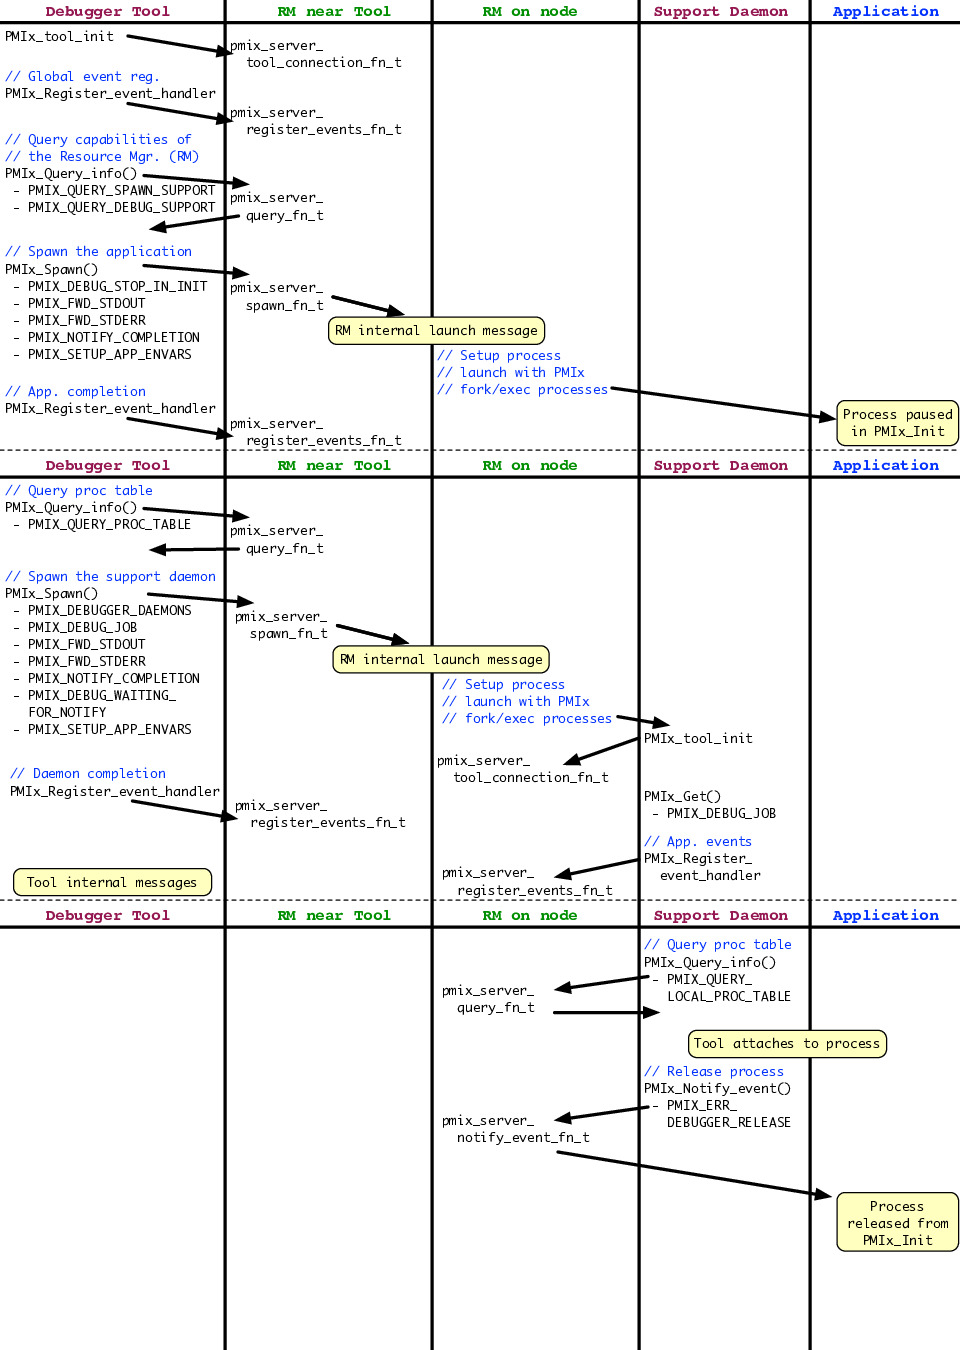
\includegraphics[width=\textwidth,height=\textheight,keepaspectratio]{figs/direct-launch}
  \end{center}
  \caption{Direct Launch}
  \label{fig:direct_launch}
\end{figure*}
\endgroup


\littleheader{Related Interfaces}

{\large \refapi{PMIx_tool_init}}
\pasteSignature{PMIx_tool_init}

{\large \refapi{PMIx_Register_event_handler}}
\pasteSignature{PMIx_Register_event_handler}

{\large \refapi{PMIx_Query_info}}
\pasteSignature{PMIx_Query_info}

{\large \refapi{PMIx_Spawn}}
\pasteSignature{PMIx_Spawn}

{\large \refapi{PMIx_Get}}
\pasteSignature{PMIx_Get}

{\large \refapi{PMIx_Notify_event}}
\pasteSignature{PMIx_Notify_event}

\littleheader{Related Attributes}

\pasteAttributeItem{PMIX_QUERY_SPAWN_SUPPORT}
\pasteAttributeItem{PMIX_QUERY_DEBUG_SUPPORT}
\pasteAttributeItem{PMIX_DEBUG_STOP_IN_INIT}
\pasteAttributeItem{PMIX_FWD_STDOUT}
\pasteAttributeItem{PMIX_FWD_STDERR}
\pasteAttributeItem{PMIX_NOTIFY_COMPLETION}
\pasteAttributeItem{PMIX_SETUP_APP_ENVARS}
\pasteAttributeItem{PMIX_DEBUGGER_DAEMONS}
\pasteAttributeItem{PMIX_DEBUG_JOB}
\pasteAttributeItem{PMIX_QUERY_LOCAL_PROC_TABLE}

\littleheader{Related Constants}

\refconst{PMIX_DEBUG_WAITING_FOR_NOTIFY} \\
\refconst{PMIX_DEBUGGER_RELEASE}

\subsubsection{Indirect-Launch Debugger Tool}

Executing a program under a tool using an intermediate launcher such as mpiexec can also be made possible. This requires some degree of coordination between the tool and the launcher. Ultimately, it is the launcher that is going to launch the application, and the tool must somehow inform it (and the application) that this is being done in a debug session so that the application knows to ``block'' until the tool attaches to it.

In this operational mode, the user invokes a tool (typically on a non-compute, or ``head'', node) that in turn uses mpiexec to launch their application – a typical command line might look like the following: \code{dbgr -dbgoption mpiexec -n 32 ./myapp}.

\begingroup
\begin{figure*}
  \begin{center}
    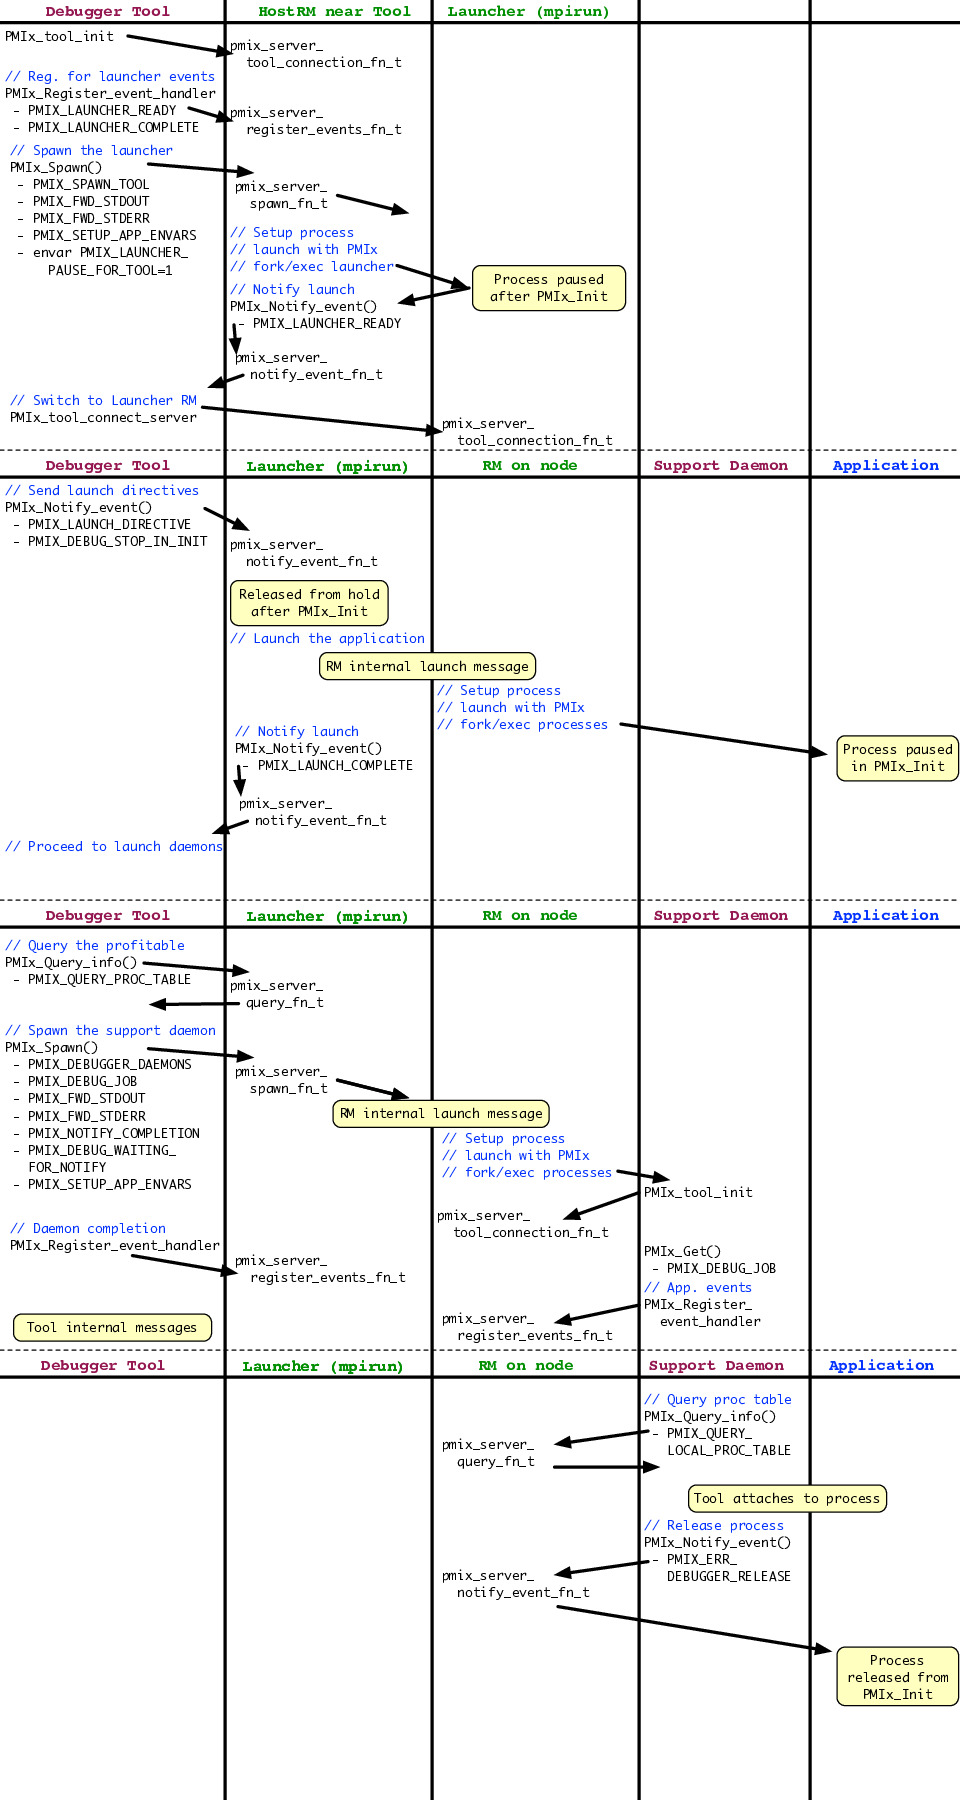
\includegraphics[width=\textwidth,height=\textheight,keepaspectratio]{figs/indirect-launch}
  \end{center}
  \caption{Indirect Launch}
  \label{fig:indirect_launch}
\end{figure*}
\endgroup


\littleheader{Related Interfaces}

{\large \refapi{PMIx_tool_init}}
\pasteSignature{PMIx_tool_init}

{\large \refapi{PMIx_Register_event_handler}}
\pasteSignature{PMIx_Register_event_handler}

{\large \refapi{PMIx_Spawn}}
\pasteSignature{PMIx_Spawn}

{\large \refapi{PMIx_Notify_event}}
\pasteSignature{PMIx_Notify_event}

{\large \refapi{PMIx_tool_attach_to_server}}
\pasteSignature{PMIx_tool_attach_to_server}

{\large \refapi{PMIx_Query_info}}
\pasteSignature{PMIx_Query_info}

{\large \refapi{PMIx_Get}}
\pasteSignature{PMIx_Get}

\littleheader{Related Attributes}

\pasteAttributeItem{PMIX_SPAWN_TOOL}
\pasteAttributeItem{PMIX_FWD_STDOUT}
\pasteAttributeItem{PMIX_FWD_STDERR}
\pasteAttributeItem{PMIX_SETUP_APP_ENVARS}
\pasteAttributeItem{PMIX_DEBUG_STOP_IN_INIT}
\pasteAttributeItem{PMIX_QUERY_PROC_TABLE}
\pasteAttributeItem{PMIX_DEBUGGER_DAEMONS}
\pasteAttributeItem{PMIX_DEBUG_JOB}
\pasteAttributeItem{PMIX_FWD_STDOUT}
\pasteAttributeItem{PMIX_FWD_STDERR}
\pasteAttributeItem{PMIX_NOTIFY_COMPLETION}
\pasteAttributeItem{PMIX_SETUP_APP_ENVARS}
\pasteAttributeItem{PMIX_DEBUG_JOB}
\pasteAttributeItem{PMIX_QUERY_LOCAL_PROC_TABLE}

\littleheader{Related Constants}

\refconst{PMIX_LAUNCHER_READY} \\
\refconst{PMIX_LAUNCH_COMPLETE} \\
\refconst{PMIX_DEBUG_WAITING_FOR_NOTIFY} \\
\refconst{PMIX_DEBUGGER_RELEASE}

\subsubsection{Attaching to a Running Job}

PMIx supports attaching to an already running parallel job in two ways.  In the first way, the main process of a tool calls \refapi{PMIx_Query_info} with the \refattr{PMIX_QUERY_PROC_TABLE} attribute.  This returns an array of structs containing the information required for \hyperref[subsubsec:process-acq]{process acquisition}.  This includes remote hostnames, executable names, and process IDs.  In the second way, every tool daemon calls \refapi{PMIx_Query_info} with the \refattr{PMIX_QUERY_LOCAL_PROC_TABLE} attribute.  This returns a similar array of structs but only for processes on the same node.

An example of this use-case may look like the following: \code{mpiexec -n32~./myApp \&\& dbgr attach \$!}.

\begingroup
\begin{figure*}
  \begin{center}
    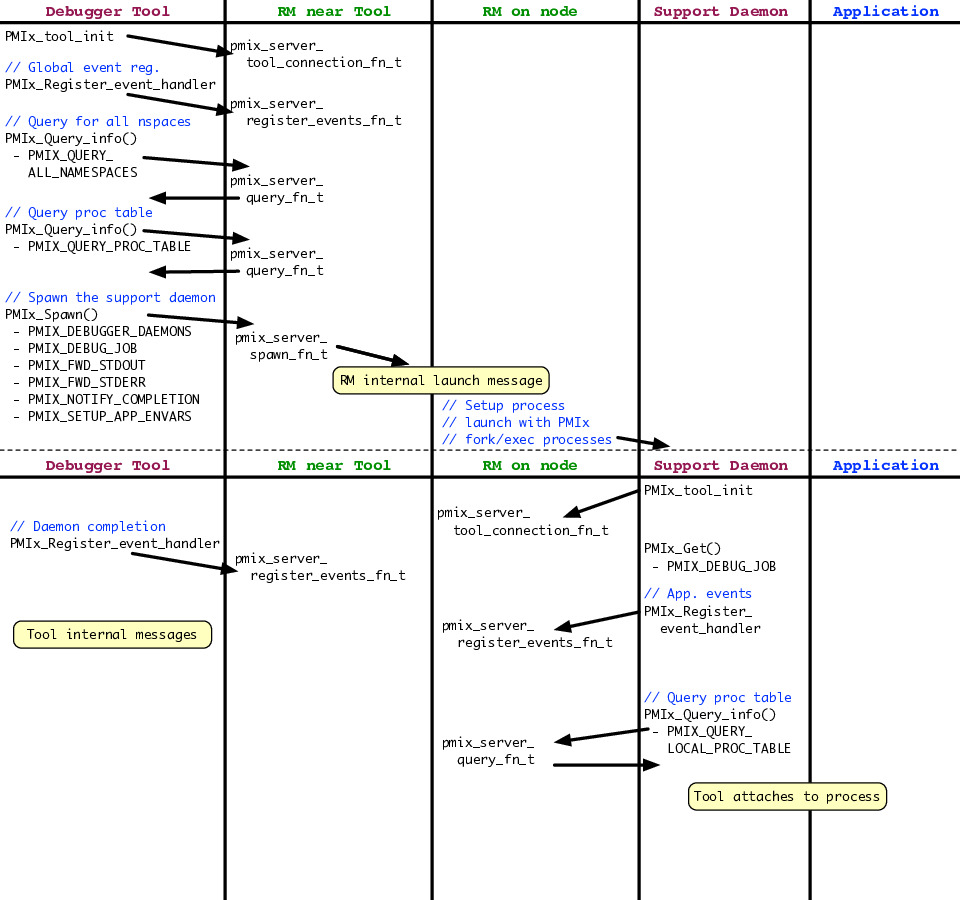
\includegraphics[width=\textwidth,height=\textheight,keepaspectratio]{figs/process-acquisition}
  \end{center}
  \caption{Attaching to a Running Job}
  \label{fig:proc_acq}
\end{figure*}
\endgroup

{\large \refapi{PMIx_tool_init}}
\pasteSignature{PMIx_tool_init}

{\large \refapi{PMIx_Register_event_handler}}
\pasteSignature{PMIx_Register_event_handler}

{\large \refapi{PMIx_Query_info}}
\pasteSignature{PMIx_Query_info}

{\large \refapi{PMIx_Spawn}}
\pasteSignature{PMIx_Spawn}

\pasteAttributeItem{PMIX_QUERY_PROC_TABLE}
\pasteAttributeItem{PMIX_DEBUGGER_DAEMONS}
\pasteAttributeItem{PMIX_DEBUG_JOB}
\pasteAttributeItem{PMIX_FWD_STDOUT}
\pasteAttributeItem{PMIX_FWD_STDERR}
\pasteAttributeItem{PMIX_NOTIFY_COMPLETION}
\pasteAttributeItem{PMIX_SETUP_APP_ENVARS}

\pasteAttributeItem{PMIX_QUERY_NAMESPACES}

\subsubsection{Tool Interaction with RM}

Tools can benefit from a mechanism by which they may interact with a local PMIx server that has opted to accept such connections along with support for tool connections to system-level PMIx servers, and a logging feature. To add support for tool connections to a specified system-level, PMIx server environments could choose to launch a set of PMIx servers to support a given allocation - these servers will (if so instructed) provide a tool rendezvous point that is tagged with their pid and typically placed in an allocation-specific temporary directory to allow for possible multi-tenancy scenarios. Supporting such operations requires that a system-level PMIx connection be provided which is not associated with a specific user or allocation. A new key has been added to direct the PMIx server to expose a rendezvous point specifically for this purpose.

{\large \refapi{PMIx_Query_info_nb}}
\pasteSignature{PMIx_Query_info_nb}

{\large \refapi{PMIx_Register_event_handler}}
\pasteSignature{PMIx_Register_event_handler}

{\large \refapi{PMIx_Deregister_event_handler}}
\pasteSignature{PMIx_Deregister_event_handler}

{\large \refapi{PMIx_Notify_event}}
\pasteSignature{PMIx_Notify_event}

{\large \refapi{PMIx_server_init}}
\pasteSignature{PMIx_server_init}

\littleheader{Job-specific events}
\code{PMIX_EVENT_JOB_LEVEL       /* debugger attached, process failure */}

\littleheader{Environment events}
\code{PMIX_EVENT_ENVIRO_LEVEL  /*ECC errors, temperature excursions */}

\littleheader{Errors detected by clients/peers}
\code{Network fabric manager detects data corruption}

\subsubsection{Environmental Parameter Directives for Applications and Launchers}

It is sometimes desirable or required that standard environmental variables (e.g., \code{PATH}, \code{LD_LIBRARY_PATH}, \code{LD_PRELOAD}) be modified prior to executing an application binary or a starter such as mpiexec - this is particularly true when tools/debuggers are used to start the application. This RFC proposes the definition of a new PMIx structure (\refstruct{pmix_envar_t}) and associated attributes for specifying such operations.

\littleheader{Related Interfaces}

{\large \refapi{PMIx_Spawn}}
\pasteSignature{PMIx_Spawn}

\littleheader{Related Structs}

\refstruct{pmix_envar_t}

\littleheader{Related Attributes}

\pasteAttributeItem{PMIX_SET_ENVAR}
\pasteAttributeItem{PMIX_ADD_ENVAR}
\pasteAttributeItem{PMIX_UNSET_ENVAR}
\pasteAttributeItem{PMIX_PREPEND_ENVAR}
\pasteAttributeItem{PMIX_APPEND_ENVAR}

Resource managers and launchers must scan for relevant directives, modifying environmental parameters as directed. Directives are to be processed in the order in which they were given, starting with job-level directives (applied to each app) followed by app-level directives.

\section{Hybrid Programming Models}
\label{app:uc-hybrid-programming-models}

\subsection{Use Case Summary}

Hybrid applications (i.e., applications that utilize more than one lprogramming model, such as an MPI application that also uses OpenMP or PGAS) are growing in popularity, especially as chips with increasingly large numbers of cores and processors proliferate. Unfortunately, the various models currently operate under the assumption that they alone control execution. This leads to conflicts in hybrid applications. Deadlock of parallel applications can occur when one model prevents the other from making progress due to lack of coordination between the multiple programming models~\cite{2016:Hamidouche}.  Sub-optimal performance can also occur due to uncoordinated division of hardware resources between the programming models~\cite{2018:Vallee,ompix-moc}. This use-case offers potential solutions to the problem by providing a pathway for programming models to coordinate their actions.

\subsection{Use Case Details}

\subsubsection{Identifying Active Programming Models}

The current state-of-the-practice for programming models to detect one another is via set environment variables.  For example, OpenMP looks for environment variables to indicate that MPI is active.  Unfortunately, this technique is not completely reliable as environment variables change over time and with new software versions.  Also, the fact that an environment variable is present doesn't guarantee that a particular programming is in active use since Resource Managers routinely set environment variables "just in case" the application needs them. PMIx provides a reliable mechanism by which each library can determine that another library is in operation.

When initializing PMIx, programming models can register themselves, including their name, version, and threading model.  This information is then cached locally and can then be read asynchronously by other programming models using PMIx's Event Notification system (see next section for more details).

This initialization mechanism also allows libraries to share knowledge of each other's resources and intended resource utilization. For example, if OpenMP knows which hardware threads that MPI is using it could potentially avoid processor and cache contention.

\littleheader{Code Example}

\pmixCodeImportC[]{sources/_autogen_/hybrid-prog-model.c_declare_model}

\littleheader{Related Interfaces}

{\large \refapi{PMIx_Init}}
\pasteSignature{PMIx_Init}

\littleheader{Related Attributes}

\pasteAttributeItem{PMIX_PROGRAMMING_MODEL}
\pasteAttributeItem{PMIX_MODEL_LIBRARY_NAME}
\pasteAttributeItem{PMIX_MODEL_LIBRARY_VERSION}
\pasteAttributeItem{PMIX_THREADING_MODEL}
\pasteAttributeItem{PMIX_MODEL_NUM_THREADS}
\pasteAttributeItem{PMIX_MODEL_NUM_CPUS}
\pasteAttributeItem{PMIX_MODEL_CPU_TYPE}
\pasteAttributeItem{PMIX_MODEL_PHASE_NAME}
\pasteAttributeItem{PMIX_MODEL_PHASE_TYPE}
\pasteAttributeItem{PMIX_MODEL_AFFINITY_POLICY}

\subsubsection{Coordinating at Runtime}

The PMIx Event Notification system provides a mechanism by which the resource manager can communicate system events to applications, thus providing applications with an opportunity to generate an appropriate response. Hybrid applications can leverage these events for cross-library coordination.

Programming models can access the information provided by other programming models during their initialization using the event notification system.  In this case, programming models should register a callback for the \refconst{PMIX_MODEL_DECLARED} event.

Programming models can also use the PMIx event notification system to communicate dynamic information, such as entering a new application phase (\pasteAttributeItem{PMIX_MODEL_PHASE_NAME}) or a change in resources used (\refconst{PMIX_MODEL_RESOURCES}).  This dynamic information can be broadcast to other programming models using the \refapi{PMIx_Notify_event} function.  Other programming models can register callback functions to run when these events occur (i.e., callback functions) using \refapi{PMIx_Register_event_handler}.

\littleheader{Code Example}

Registering a callback to run when another programming model initializes:
\pmixCodeImportC[]{sources/_autogen_/hybrid-prog-model.c_declare_model_cb}


Notifying an event:
\pmixCodeImportC[]{sources/_autogen_/hybrid-prog-model.c_notify_event}

\littleheader{Related Interfaces and Constants}

{\large \refapi{PMIx_Notify_event}}
\pasteSignature{PMIx_Notify_event}

\refconst{PMIX_MODEL_DECLARED} \\
\refconst{PMIX_MODEL_RESOURCES} \\
\refconst{PMIX_OPENMP_PARALLEL_ENTERED} \\
\refconst{PMIX_OPENMP_PARALLEL_EXITED} \\

{\large \refapi{PMIx_Register_event_handler}}
\pasteSignature{PMIx_Register_event_handler}

{\large \refapi{pmix_event_notification_cbfunc_fn_t}}
\pasteSignature{pmix_event_notification_cbfunc_fn_t}

\refconst{PMIX_EVENT_ACTION_COMPLETE}



\subsubsection{Coordinating at Runtime with Multiple Event Handlers}

Coordinating with a threading library such as OpenMP creates the need for separate event handlers for threads of the same process.  For example in an MPI+OpenMP hybrid application, the MPI thread and the main OpenMP thread may both want to be notified anytime an OpenMP worker thread enters a parallel region.  This requiring support for multiple threads to potentially register different event handlers against the same status code.

Multiple event handlers registered against the same event are processed in a chain-like manner based on the order in which they were registered, as modified by directive. Registrations against specific event codes are processed first, followed by registrations against multiple event codes and then any default registrations. At each point in the chain, an event handler is called by the PMIx progress thread and given a function to call when that handler has completed its operation. The handler callback notifies PMIx that the handler is done, returning a status code to indicate the result of its work. The results are appended to the array of prior results, with the returned values combined into an array within a single pmix_info_t as follows:
\begin{itemize}
\item \texttt{array[0]}: the event handler name provided at registration (may be an empty field if a string name was not given) will be in the key, with the pmix_status_t value returned by the handler
\item \texttt{array[*]}: the array of results returned by the handler, if any.
\end{itemize}

The current PMIx standard does not actually specify a default ordering for event handlers as they are being registered. However, it does include an inherent ordering for invocation. Specifically, PMIx stipulates that handlers be called in the following categorical order:

\begin{itemize}
\item single status event handlers - i.e., handlers that were registered against a single specific status.
\item multi status event handlers - those registered against more than one specific status
\item default event handlers - those registered against no specific status
\end{itemize}

\littleheader{Code Example}

From the OpenMP master thread:

\pmixCodeImportC[]{sources/_autogen_/hybrid-prog-model.c_omp_thread}

From the MPI thread:

\pmixCodeImportC[]{sources/_autogen_/hybrid-prog-model.c_mpi_thread}

\littleheader{Related Interfaces, Attributes, and Constants}

{\large \refapi{PMIx_Register_event_handler}}
\pasteSignature{PMIx_Register_event_handler}

\pasteAttributeItem{PMIX_EVENT_HDLR_NAME}
\pasteAttributeItem{PMIX_EVENT_HDLR_FIRST}
\pasteAttributeItem{PMIX_EVENT_HDLR_LAST}
\pasteAttributeItem{PMIX_EVENT_HDLR_FIRST_IN_CATEGORY}
\pasteAttributeItem{PMIX_EVENT_HDLR_LAST_IN_CATEGORY}
\pasteAttributeItem{PMIX_EVENT_HDLR_BEFORE}
\pasteAttributeItem{PMIX_EVENT_HDLR_AFTER}
\pasteAttributeItem{PMIX_EVENT_HDLR_APPEND}

{\large \refapi{pmix_event_notification_cbfunc_fn_t}}
\pasteSignature{pmix_event_notification_cbfunc_fn_t}

\refconst{PMIX_EVENT_NO_ACTION_TAKEN} \\
\refconst{PMIX_EVENT_PARTIAL_ACTION_TAKEN} \\
\refconst{PMIX_EVENT_ACTION_DEFERRED} \\

%%%%%%%%%%%%%%%%%%%%%%%%%%%%%%%%%%%%%%%%%%%%%%%%%
>>>>>>> 1bfbca4 (use cases: add debugging chapter)


% Revisions, Acknowledgements
    % Revisions
    \input{Chap_Revisions.tex}

    \input{Acknowledgements}

%
% Bibliography
%
	\nolinenumbers
	\bibliography{pmix-standard}{}
	\addcontentsline{toc}{chapter}{Bibliography}
	\bibliographystyle{plain}

%
% Index
%
	\nolinenumbers

	\indexprologue{General terms and other items not induced in the other indices.}
	\printindex

	%\indexprologue{Functions}
	\printindex[index_api]

	%\indexprologue{Macros}
	\printindex[index_macro]

	%\indexprologue{Data structures}
	\printindex[index_struct]

	%\indexprologue{Constants}
	\printindex[index_const]

    %\indexprologue{Envars}
    \printindex[index_envars]

	%\indexprologue{Attributes}
	\printindex[index_attribute]


\end{document}

%%%%%%%%%%%%%%%%%%%%%%%%%%%%%%%%%%%%%%%%%%%%%%%%%
